\documentclass[11pt]{article}
% generated by Madoko, version 1.1.4
%mdk-data-line={1}


\usepackage[heading-base={2},section-num={False},bib-label={hide},fontspec={True}]{madoko2}
\usepackage[top=1in, bottom=1.25in, left=1in, right=1in]{geometry}
\usepackage{fancyhdr}
%mdk-data-line={11}

  \setlength{\headheight}{30pt}
  \setlength{\emergencystretch}{2em}

\begin{document}



{\mdfontfamily{UtopiaStd-Regular}
%mdk-data-line={203}
\mdxtitleblockstart{}
%mdk-data-line={203}
\mdxtitle{{\sffamily{\bfseries\mdline{203}P4Runtime Specification}}}%mdk

%mdk-data-line={206}
\mdxtitlenote{{\sffamily{\bfseries\mdline{206}version 1.0.0}}}%mdk
\mdxauthorstart{}
%mdk-data-line={211}
\mdxauthorname{\mdline{211}The P4.org API Working Group}%mdk
\mdxauthorend
%mdk-data-line={220}
\mdxtitlefooter{{\sffamily{\bfseries\mdline{220}2019-10-28}}}%mdk
\mdtitleauthorrunning{}{}\mdxtitleblockend%mdk

%mdk-data-line={205}
\begin{abstract}%mdk

%mdk-data-line={206}
\noindent\mdline{206}P4 is a language for programming the data plane of network devices. The
P4Runtime API is a control plane specification for controlling the data plane
elements of a device defined or described by a P4 program. This document
provides a precise definition of the P4Runtime API. The target audience for this
document includes developers who want to write controller applications for P4
devices or switches.%mdk
%mdk
\end{abstract}%mdk
\mdline{214}
\begin{mdtoc}%mdk

\section*{Contents}\label{sec-contents}%mdk%mdk

\begin{mdtocblock}%mdk

\mdtocitemx{sec-introduction-and-scope}{\mdref{sec-introduction-and-scope}{1.\hspace*{0.5em}Introduction and Scope}}%mdk

\begin{mdtocblock}%mdk

\mdtocitemx{sec-p4-language-version-applicability}{\mdref{sec-p4-language-version-applicability}{1.1.\hspace*{0.5em}P4 Language Version Applicability}}%mdk

\mdtocitemx{sec-in-scope}{\mdref{sec-in-scope}{1.2.\hspace*{0.5em}In Scope}}%mdk

\mdtocitemx{sec-not-in-scope}{\mdref{sec-not-in-scope}{1.3.\hspace*{0.5em}Not In Scope}}%mdk
%mdk
\end{mdtocblock}%mdk

\mdtocitemx{sec-terms-and-definitions}{\mdref{sec-terms-and-definitions}{2.\hspace*{0.5em}Terms and Definitions}}%mdk

\mdtocitemx{sec-reference-architecture}{\mdref{sec-reference-architecture}{3.\hspace*{0.5em}Reference Architecture}}%mdk

\begin{mdtocblock}%mdk

\mdtocitemx{sec-idealized-workflow}{\mdref{sec-idealized-workflow}{3.1.\hspace*{0.5em}Idealized Workflow}}%mdk

\mdtocitemx{sec-p4-as-behavioral-description-language}{\mdref{sec-p4-as-behavioral-description-language}{3.2.\hspace*{0.5em}P4 as a Behavioral Description Language}}%mdk

\mdtocitemx{sec-alternative-workflows}{\mdref{sec-alternative-workflows}{3.3.\hspace*{0.5em}Alternative Workflows}}%mdk

\begin{mdtocblock}%mdk

\mdtocitemx{sec-p4-source-available-compiled-into-p4info-but-not-compiled-into-p4-device-config}{\mdref{sec-p4-source-available-compiled-into-p4info-but-not-compiled-into-p4-device-config}{3.3.1.\hspace*{0.5em}P4 Source Available, Compiled into P4Info but not Compiled into P4 Device Config}}%mdk

\mdtocitemx{sec-no-p4-source-available-p4info-available}{\mdref{sec-no-p4-source-available-p4info-available}{3.3.2.\hspace*{0.5em}No P4 Source Available, P4Info Available}}%mdk

\mdtocitemx{sec-partial-p4info-and-p4-source-are-available}{\mdref{sec-partial-p4info-and-p4-source-are-available}{3.3.3.\hspace*{0.5em}Partial P4Info and P4 Source are Available}}%mdk

\mdtocitemx{sec-p4info-role-based-subsets}{\mdref{sec-p4info-role-based-subsets}{3.3.4.\hspace*{0.5em}P4Info Role-Based Subsets}}%mdk
%mdk
\end{mdtocblock}%mdk

\mdtocitemx{sec-restarts}{\mdref{sec-restarts}{3.4.\hspace*{0.5em}P4Runtime State Across Restarts}}%mdk
%mdk
\end{mdtocblock}%mdk

\mdtocitemx{sec-controller-use-cases}{\mdref{sec-controller-use-cases}{4.\hspace*{0.5em}Controller Use-cases}}%mdk

\begin{mdtocblock}%mdk

\mdtocitemx{sec-single-embedded-controller}{\mdref{sec-single-embedded-controller}{4.1.\hspace*{0.5em}Single Embedded Controller}}%mdk

\mdtocitemx{sec-single-remote-controller}{\mdref{sec-single-remote-controller}{4.2.\hspace*{0.5em}Single Remote Controller}}%mdk

\mdtocitemx{sec-embedded-single-remote-controller}{\mdref{sec-embedded-single-remote-controller}{4.3.\hspace*{0.5em}Embedded + Single Remote Controller}}%mdk

\mdtocitemx{sec-embedded-two-remote-controllers}{\mdref{sec-embedded-two-remote-controllers}{4.4.\hspace*{0.5em}Embedded + Two Remote Controllers}}%mdk

\mdtocitemx{sec-embedded-controller-two-high-availability-remote-controllers}{\mdref{sec-embedded-controller-two-high-availability-remote-controllers}{4.5.\hspace*{0.5em}Embedded Controller + Two High-Availability Remote Controllers}}%mdk
%mdk
\end{mdtocblock}%mdk

\mdtocitemx{sec-master-slave-arbitration-and-controller-replication}{\mdref{sec-master-slave-arbitration-and-controller-replication}{5.\hspace*{0.5em}Master-Slave Arbitration and Controller Replication}}%mdk

\begin{mdtocblock}%mdk

\mdtocitemx{sec-default-role}{\mdref{sec-default-role}{5.1.\hspace*{0.5em}Default Role}}%mdk

\mdtocitemx{sec-arbitration-role-config}{\mdref{sec-arbitration-role-config}{5.2.\hspace*{0.5em}Role Config}}%mdk

\mdtocitemx{sec-mastership-updates}{\mdref{sec-mastership-updates}{5.3.\hspace*{0.5em}Rules for Handling \mdcode{{\mdfontfamily{LuxiMono}{\mdfontsize{\dimfont{0.75}}MasterArbitrationUpdate}}} Messages Received from Controllers}}%mdk

\mdtocitemx{sec-mastership-notification}{\mdref{sec-mastership-notification}{5.4.\hspace*{0.5em}Mastership Notifications}}%mdk
%mdk
\end{mdtocblock}%mdk

\mdtocitemx{sec-the-p4info-message}{\mdref{sec-the-p4info-message}{6.\hspace*{0.5em}The P4Info Message}}%mdk

\begin{mdtocblock}%mdk

\mdtocitemx{sec-common-messages}{\mdref{sec-common-messages}{6.1.\hspace*{0.5em}Common Messages}}%mdk

\begin{mdtocblock}%mdk

\mdtocitemx{sec-documentation-message}{\mdref{sec-documentation-message}{6.1.1.\hspace*{0.5em}\mdcode{{\mdfontfamily{LuxiMono}{\mdfontsize{\dimfont{0.75}}Documentation}}} Message}}%mdk

\mdtocitemx{sec-preamble-message}{\mdref{sec-preamble-message}{6.1.2.\hspace*{0.5em}\mdcode{{\mdfontfamily{LuxiMono}{\mdfontsize{\dimfont{0.75}}Preamble}}} Message}}%mdk

\mdtocitemx{sec-annotating-p4-entities-with-documentation}{\mdref{sec-annotating-p4-entities-with-documentation}{6.1.3.\hspace*{0.5em}Annotating P4 Entities with \mdcode{{\mdfontfamily{LuxiMono}{\mdfontsize{\dimfont{0.75}}Documentation}}}}}%mdk
%mdk
\end{mdtocblock}%mdk

\mdtocitemx{sec-pkginfo-message}{\mdref{sec-pkginfo-message}{6.2.\hspace*{0.5em}\mdcode{{\mdfontfamily{LuxiMono}{\mdfontsize{\dimfont{0.75}}PkgInfo}}} Message}}%mdk

\begin{mdtocblock}%mdk

\mdtocitemx{sec-annotating-p4-code-with-pkginfo}{\mdref{sec-annotating-p4-code-with-pkginfo}{6.2.1.\hspace*{0.5em}Annotating P4 code with PkgInfo}}%mdk
%mdk
\end{mdtocblock}%mdk

\mdtocitemx{sec-id-allocation}{\mdref{sec-id-allocation}{6.3.\hspace*{0.5em}ID Allocation for P4Info Objects}}%mdk

\mdtocitemx{sec-p4info-objects}{\mdref{sec-p4info-objects}{6.4.\hspace*{0.5em}P4Info Objects}}%mdk

\begin{mdtocblock}%mdk

\mdtocitemx{sec-table}{\mdref{sec-table}{6.4.1.\hspace*{0.5em}\mdcode{{\mdfontfamily{LuxiMono}{\mdfontsize{\dimfont{0.75}}Table}}}}}%mdk

\mdtocitemx{sec-action}{\mdref{sec-action}{6.4.2.\hspace*{0.5em}\mdcode{{\mdfontfamily{LuxiMono}{\mdfontsize{\dimfont{0.75}}Action}}}}}%mdk

\mdtocitemx{sec-p4info-action-profile}{\mdref{sec-p4info-action-profile}{6.4.3.\hspace*{0.5em}\mdcode{{\mdfontfamily{LuxiMono}{\mdfontsize{\dimfont{0.75}}ActionProfile}}}}}%mdk

\mdtocitemx{sec-counter-directcounter}{\mdref{sec-counter-directcounter}{6.4.4.\hspace*{0.5em}\mdcode{{\mdfontfamily{LuxiMono}{\mdfontsize{\dimfont{0.75}}Counter}}} \& \mdcode{{\mdfontfamily{LuxiMono}{\mdfontsize{\dimfont{0.75}}DirectCounter}}}}}%mdk

\mdtocitemx{sec-meter-directmeter}{\mdref{sec-meter-directmeter}{6.4.5.\hspace*{0.5em}\mdcode{{\mdfontfamily{LuxiMono}{\mdfontsize{\dimfont{0.75}}Meter}}} \& \mdcode{{\mdfontfamily{LuxiMono}{\mdfontsize{\dimfont{0.75}}DirectMeter}}}}}%mdk

\mdtocitemx{sec-controller-packet-meta}{\mdref{sec-controller-packet-meta}{6.4.6.\hspace*{0.5em}\mdcode{{\mdfontfamily{LuxiMono}{\mdfontsize{\dimfont{0.75}}ControllerPacketMetadata}}}}}%mdk

\mdtocitemx{sec-valueset}{\mdref{sec-valueset}{6.4.7.\hspace*{0.5em}\mdcode{{\mdfontfamily{LuxiMono}{\mdfontsize{\dimfont{0.75}}ValueSet}}}}}%mdk

\mdtocitemx{sec-register}{\mdref{sec-register}{6.4.8.\hspace*{0.5em}\mdcode{{\mdfontfamily{LuxiMono}{\mdfontsize{\dimfont{0.75}}Register}}}}}%mdk

\mdtocitemx{sec-digest}{\mdref{sec-digest}{6.4.9.\hspace*{0.5em}\mdcode{{\mdfontfamily{LuxiMono}{\mdfontsize{\dimfont{0.75}}Digest}}}}}%mdk

\mdtocitemx{sec-p4info-extern}{\mdref{sec-p4info-extern}{6.4.10.\hspace*{0.5em}\mdcode{{\mdfontfamily{LuxiMono}{\mdfontsize{\dimfont{0.75}}Extern}}}}}%mdk
%mdk
\end{mdtocblock}%mdk

\mdtocitemx{sec-support-for-arbitrary-p4-types-with-p4typeinfo}{\mdref{sec-support-for-arbitrary-p4-types-with-p4typeinfo}{6.5.\hspace*{0.5em}Support for Arbitrary P4 Types with P4TypeInfo}}%mdk
%mdk
\end{mdtocblock}%mdk

\mdtocitemx{sec-p4-fwd-pipe-config}{\mdref{sec-p4-fwd-pipe-config}{7.\hspace*{0.5em}P4 Forwarding-Pipeline Configuration}}%mdk

\mdtocitemx{sec-general-principles-for-message-formatting}{\mdref{sec-general-principles-for-message-formatting}{8.\hspace*{0.5em}General Principles for Message Formatting}}%mdk

\begin{mdtocblock}%mdk

\mdtocitemx{sec-set-unset-protobuf-field}{\mdref{sec-set-unset-protobuf-field}{8.1.\hspace*{0.5em}Set / Unset Protobuf Field}}%mdk

\mdtocitemx{sec-read-write-symmetry}{\mdref{sec-read-write-symmetry}{8.2.\hspace*{0.5em}Read-Write Symmetry}}%mdk

\mdtocitemx{sec-zero-as-reserved-value}{\mdref{sec-zero-as-reserved-value}{8.3.\hspace*{0.5em}Zero as Reserved Value}}%mdk

\mdtocitemx{sec-bytestrings}{\mdref{sec-bytestrings}{8.4.\hspace*{0.5em}Bytestrings}}%mdk

\mdtocitemx{sec-representation-of-arbitrary-p4-types}{\mdref{sec-representation-of-arbitrary-p4-types}{8.5.\hspace*{0.5em}Representation of Arbitrary P4 Types}}%mdk

\begin{mdtocblock}%mdk

\mdtocitemx{sec-problem-statement}{\mdref{sec-problem-statement}{8.5.1.\hspace*{0.5em}Problem Statement}}%mdk

\mdtocitemx{sec-p4-type-specifications-in-p4infoproto}{\mdref{sec-p4-type-specifications-in-p4infoproto}{8.5.2.\hspace*{0.5em}P4 Type Specifications in p4info.proto}}%mdk

\mdtocitemx{sec-p4data-in-p4runtime-proto}{\mdref{sec-p4data-in-p4runtime-proto}{8.5.3.\hspace*{0.5em}\mdcode{{\mdfontfamily{LuxiMono}{\mdfontsize{\dimfont{0.75}}P4Data}}} in p4runtime.proto}}%mdk

\mdtocitemx{sec-example}{\mdref{sec-example}{8.5.4.\hspace*{0.5em}Example}}%mdk

\mdtocitemx{sec-enum-serializable-enum-and-error}{\mdref{sec-enum-serializable-enum-and-error}{8.5.5.\hspace*{0.5em}\mdcode{{\mdfontfamily{LuxiMono}{\mdfontsize{\dimfont{0.75}}enum}}}, serializable \mdcode{{\mdfontfamily{LuxiMono}{\mdfontsize{\dimfont{0.75}}enum}}} and \mdcode{{\mdfontfamily{LuxiMono}{\mdfontsize{\dimfont{0.75}}error}}}}}%mdk

\mdtocitemx{sec-user-defined-types}{\mdref{sec-user-defined-types}{8.5.6.\hspace*{0.5em}User-defined types}}%mdk

\mdtocitemx{sec-trade-off-for-v10-release}{\mdref{sec-trade-off-for-v10-release}{8.5.7.\hspace*{0.5em}Trade-off for v1.0 Release}}%mdk
%mdk
\end{mdtocblock}%mdk
%mdk
\end{mdtocblock}%mdk

\mdtocitemx{sec-p4-entity-msgs}{\mdref{sec-p4-entity-msgs}{9.\hspace*{0.5em}P4 Entity Messages}}%mdk

\begin{mdtocblock}%mdk

\mdtocitemx{sec-table-entry}{\mdref{sec-table-entry}{9.1.\hspace*{0.5em}\mdcode{{\mdfontfamily{LuxiMono}{\mdfontsize{\dimfont{0.75}}TableEntry}}}}}%mdk

\begin{mdtocblock}%mdk

\mdtocitemx{sec-match-format}{\mdref{sec-match-format}{9.1.1.\hspace*{0.5em}Match Format}}%mdk

\mdtocitemx{sec-action-specification}{\mdref{sec-action-specification}{9.1.2.\hspace*{0.5em}Action Specification}}%mdk

\mdtocitemx{sec-default-entry}{\mdref{sec-default-entry}{9.1.3.\hspace*{0.5em}Default Entry}}%mdk

\mdtocitemx{sec-constant-tables}{\mdref{sec-constant-tables}{9.1.4.\hspace*{0.5em}Constant Tables}}%mdk

\mdtocitemx{sec-table-wildcard-reads}{\mdref{sec-table-wildcard-reads}{9.1.5.\hspace*{0.5em}Wildcard Reads}}%mdk

\mdtocitemx{sec-direct-resources}{\mdref{sec-direct-resources}{9.1.6.\hspace*{0.5em}Direct Resources}}%mdk

\mdtocitemx{sec-idle-timeout}{\mdref{sec-idle-timeout}{9.1.7.\hspace*{0.5em}Idle-timeout}}%mdk
%mdk
\end{mdtocblock}%mdk

\mdtocitemx{sec-action-profile-member-and-group}{\mdref{sec-action-profile-member-and-group}{9.2.\hspace*{0.5em}\mdcode{{\mdfontfamily{LuxiMono}{\mdfontsize{\dimfont{0.75}}ActionProfileMember}}} \& \mdcode{{\mdfontfamily{LuxiMono}{\mdfontsize{\dimfont{0.75}}ActionProfileGroup}}}}}%mdk

\begin{mdtocblock}%mdk

\mdtocitemx{sec-action-profile-member-programming}{\mdref{sec-action-profile-member-programming}{9.2.1.\hspace*{0.5em}Action Profile Member Programming}}%mdk

\mdtocitemx{sec-action-profile-group-programming}{\mdref{sec-action-profile-group-programming}{9.2.2.\hspace*{0.5em}Action Profile Group Programming}}%mdk

\mdtocitemx{sec-oneshot}{\mdref{sec-oneshot}{9.2.3.\hspace*{0.5em}One Shot Action Selector Programming}}%mdk

\mdtocitemx{sec-constraints-on-action-selector-programming}{\mdref{sec-constraints-on-action-selector-programming}{9.2.4.\hspace*{0.5em}Constraints on action selector programming}}%mdk
%mdk
\end{mdtocblock}%mdk

\mdtocitemx{sec-counterentry-directcounterentry}{\mdref{sec-counterentry-directcounterentry}{9.3.\hspace*{0.5em}\mdcode{{\mdfontfamily{LuxiMono}{\mdfontsize{\dimfont{0.75}}CounterEntry}}} \& \mdcode{{\mdfontfamily{LuxiMono}{\mdfontsize{\dimfont{0.75}}DirectCounterEntry}}}}}%mdk

\begin{mdtocblock}%mdk

\mdtocitemx{sec-directcounterentry}{\mdref{sec-directcounterentry}{9.3.1.\hspace*{0.5em}\mdcode{{\mdfontfamily{LuxiMono}{\mdfontsize{\dimfont{0.75}}DirectCounterEntry}}}}}%mdk

\mdtocitemx{sec-counterentry}{\mdref{sec-counterentry}{9.3.2.\hspace*{0.5em}\mdcode{{\mdfontfamily{LuxiMono}{\mdfontsize{\dimfont{0.75}}CounterEntry}}}}}%mdk
%mdk
\end{mdtocblock}%mdk

\mdtocitemx{sec-meterentry-directmeterentry}{\mdref{sec-meterentry-directmeterentry}{9.4.\hspace*{0.5em}\mdcode{{\mdfontfamily{LuxiMono}{\mdfontsize{\dimfont{0.75}}MeterEntry}}} \& \mdcode{{\mdfontfamily{LuxiMono}{\mdfontsize{\dimfont{0.75}}DirectMeterEntry}}}}}%mdk

\begin{mdtocblock}%mdk

\mdtocitemx{sec-directmeterentry}{\mdref{sec-directmeterentry}{9.4.1.\hspace*{0.5em}\mdcode{{\mdfontfamily{LuxiMono}{\mdfontsize{\dimfont{0.75}}DirectMeterEntry}}}}}%mdk

\mdtocitemx{sec-meterentry}{\mdref{sec-meterentry}{9.4.2.\hspace*{0.5em}\mdcode{{\mdfontfamily{LuxiMono}{\mdfontsize{\dimfont{0.75}}MeterEntry}}}}}%mdk
%mdk
\end{mdtocblock}%mdk

\mdtocitemx{sec-packetreplicationengineentry}{\mdref{sec-packetreplicationengineentry}{9.5.\hspace*{0.5em}\mdcode{{\mdfontfamily{LuxiMono}{\mdfontsize{\dimfont{0.75}}PacketReplicationEngineEntry}}}}}%mdk

\begin{mdtocblock}%mdk

\mdtocitemx{sec-multicastgroupentry}{\mdref{sec-multicastgroupentry}{9.5.1.\hspace*{0.5em}\mdcode{{\mdfontfamily{LuxiMono}{\mdfontsize{\dimfont{0.75}}MulticastGroupEntry}}}}}%mdk

\mdtocitemx{sec-clonesessionentry}{\mdref{sec-clonesessionentry}{9.5.2.\hspace*{0.5em}\mdcode{{\mdfontfamily{LuxiMono}{\mdfontsize{\dimfont{0.75}}CloneSessionEntry}}}}}%mdk
%mdk
\end{mdtocblock}%mdk

\mdtocitemx{sec-valuesetentry}{\mdref{sec-valuesetentry}{9.6.\hspace*{0.5em}\mdcode{{\mdfontfamily{LuxiMono}{\mdfontsize{\dimfont{0.75}}ValueSetEntry}}}}}%mdk

\mdtocitemx{sec-registerentry}{\mdref{sec-registerentry}{9.7.\hspace*{0.5em}\mdcode{{\mdfontfamily{LuxiMono}{\mdfontsize{\dimfont{0.75}}RegisterEntry}}}}}%mdk

\mdtocitemx{sec-digestentry}{\mdref{sec-digestentry}{9.8.\hspace*{0.5em}\mdcode{{\mdfontfamily{LuxiMono}{\mdfontsize{\dimfont{0.75}}DigestEntry}}}}}%mdk

\mdtocitemx{sec-extern-entry}{\mdref{sec-extern-entry}{9.9.\hspace*{0.5em}\mdcode{{\mdfontfamily{LuxiMono}{\mdfontsize{\dimfont{0.75}}ExternEntry}}}}}%mdk
%mdk
\end{mdtocblock}%mdk

\mdtocitemx{sec-error-reporting-messages}{\mdref{sec-error-reporting-messages}{10.\hspace*{0.5em}Error Reporting Messages}}%mdk

\mdtocitemx{sec-atomicity-of-individual-write-and-read-operations}{\mdref{sec-atomicity-of-individual-write-and-read-operations}{11.\hspace*{0.5em}Atomicity of Individual \mdcode{{\mdfontfamily{LuxiMono}{\mdfontsize{\dimfont{0.75}}Write}}} and \mdcode{{\mdfontfamily{LuxiMono}{\mdfontsize{\dimfont{0.75}}Read}}} Operations}}%mdk

\mdtocitemx{sec-write-rpc}{\mdref{sec-write-rpc}{12.\hspace*{0.5em}\mdcode{{\mdfontfamily{LuxiMono}{\mdfontsize{\dimfont{0.75}}Write}}} RPC}}%mdk

\begin{mdtocblock}%mdk

\mdtocitemx{sec-batching-and-ordering-of-updates}{\mdref{sec-batching-and-ordering-of-updates}{12.1.\hspace*{0.5em}Batching and Ordering of Updates}}%mdk

\mdtocitemx{sec-batch-atomicity}{\mdref{sec-batch-atomicity}{12.2.\hspace*{0.5em}Batch Atomicity}}%mdk

\mdtocitemx{sec-error-reporting}{\mdref{sec-error-reporting}{12.3.\hspace*{0.5em}Error Reporting}}%mdk
%mdk
\end{mdtocblock}%mdk

\mdtocitemx{sec-read-rpc}{\mdref{sec-read-rpc}{13.\hspace*{0.5em}\mdcode{{\mdfontfamily{LuxiMono}{\mdfontsize{\dimfont{0.75}}Read}}} RPC}}%mdk

\begin{mdtocblock}%mdk

\mdtocitemx{sec-nomenclature}{\mdref{sec-nomenclature}{13.1.\hspace*{0.5em}Nomenclature}}%mdk

\mdtocitemx{sec-wildcard-reads}{\mdref{sec-wildcard-reads}{13.2.\hspace*{0.5em}Wildcard Reads}}%mdk

\mdtocitemx{sec-batch-processing}{\mdref{sec-batch-processing}{13.3.\hspace*{0.5em}Batch Processing}}%mdk

\begin{mdtocblock}%mdk

\mdtocitemx{sec-example}{\mdref{sec-example}{13.3.1.\hspace*{0.5em}Example}}%mdk
%mdk
\end{mdtocblock}%mdk

\mdtocitemx{sec-parallelism-of-read-and-write-requests}{\mdref{sec-parallelism-of-read-and-write-requests}{13.4.\hspace*{0.5em}Parallelism of Read and Write Requests}}%mdk
%mdk
\end{mdtocblock}%mdk

\mdtocitemx{sec-setforwardingpipelineconfig-rpc}{\mdref{sec-setforwardingpipelineconfig-rpc}{14.\hspace*{0.5em}\mdcode{{\mdfontfamily{LuxiMono}{\mdfontsize{\dimfont{0.75}}SetForwardingPipelineConfig}}} RPC}}%mdk

\mdtocitemx{sec-getforwardingpipelineconfig-rpc}{\mdref{sec-getforwardingpipelineconfig-rpc}{15.\hspace*{0.5em}\mdcode{{\mdfontfamily{LuxiMono}{\mdfontsize{\dimfont{0.75}}GetForwardingPipelineConfig}}} RPC}}%mdk

\mdtocitemx{sec-p4runtime-stream-messages}{\mdref{sec-p4runtime-stream-messages}{16.\hspace*{0.5em}P4Runtime Stream Messages}}%mdk

\begin{mdtocblock}%mdk

\mdtocitemx{sec-packet-i_o}{\mdref{sec-packet-i_o}{16.1.\hspace*{0.5em}Packet I/O}}%mdk

\mdtocitemx{sec-master-arbitration-update}{\mdref{sec-master-arbitration-update}{16.2.\hspace*{0.5em}Master Arbitration Update}}%mdk

\mdtocitemx{sec-digest-messages}{\mdref{sec-digest-messages}{16.3.\hspace*{0.5em}Digest Messages}}%mdk

\mdtocitemx{sec-table-idle-timeout-notification}{\mdref{sec-table-idle-timeout-notification}{16.4.\hspace*{0.5em}Table Idle Timeout Notification}}%mdk

\mdtocitemx{sec-architecture-specific-notifications}{\mdref{sec-architecture-specific-notifications}{16.5.\hspace*{0.5em}Architecture-Specific Notifications}}%mdk

\mdtocitemx{sec-stream-error-reporting}{\mdref{sec-stream-error-reporting}{16.6.\hspace*{0.5em}Stream Error Reporting}}%mdk

\begin{mdtocblock}%mdk

\mdtocitemx{sec-examples-of-streamerror-messages}{\mdref{sec-examples-of-streamerror-messages}{16.6.1.\hspace*{0.5em}Examples of \mdcode{{\mdfontfamily{LuxiMono}{\mdfontsize{\dimfont{0.75}}StreamError}}} Messages}}%mdk
%mdk
\end{mdtocblock}%mdk
%mdk
\end{mdtocblock}%mdk

\mdtocitemx{sec-portability-considerations}{\mdref{sec-portability-considerations}{17.\hspace*{0.5em}Portability Considerations}}%mdk

\begin{mdtocblock}%mdk

\mdtocitemx{sec-psa-metadata-translation}{\mdref{sec-psa-metadata-translation}{17.1.\hspace*{0.5em}PSA Metadata Translation}}%mdk

\begin{mdtocblock}%mdk

\mdtocitemx{sec-translation-of-port-numbers}{\mdref{sec-translation-of-port-numbers}{17.1.1.\hspace*{0.5em}Translation of Port Numbers}}%mdk

\mdtocitemx{sec-translation-of-packet-io-header-fields}{\mdref{sec-translation-of-packet-io-header-fields}{17.1.2.\hspace*{0.5em}Translation of Packet-IO Header Fields}}%mdk

\mdtocitemx{sec-translation-of-match-fields}{\mdref{sec-translation-of-match-fields}{17.1.3.\hspace*{0.5em}Translation of Match Fields}}%mdk

\mdtocitemx{sec-translation-of-action-parameters}{\mdref{sec-translation-of-action-parameters}{17.1.4.\hspace*{0.5em}Translation of Action Parameters}}%mdk

\mdtocitemx{sec-port-translation-for-psa-extern-apis}{\mdref{sec-port-translation-for-psa-extern-apis}{17.1.5.\hspace*{0.5em}Port Translation for PSA Extern APIs}}%mdk

\mdtocitemx{sec-using-port-as-an-index-to-a-register-indirect-counter-or-indirect-meter}{\mdref{sec-using-port-as-an-index-to-a-register-indirect-counter-or-indirect-meter}{17.1.6.\hspace*{0.5em}Using Port as an Index to a Register, Indirect Counter or Indirect Meter}}%mdk
%mdk
\end{mdtocblock}%mdk
%mdk
\end{mdtocblock}%mdk

\mdtocitemx{sec-p4runtime-versioning}{\mdref{sec-p4runtime-versioning}{18.\hspace*{0.5em}P4Runtime Versioning}}%mdk

\mdtocitemx{sec-extending-p4runtime}{\mdref{sec-extending-p4runtime}{19.\hspace*{0.5em}Extending P4Runtime for non-PSA Architectures}}%mdk

\begin{mdtocblock}%mdk

\mdtocitemx{sec-extending-p4runtime-for-architecture-specific-externs}{\mdref{sec-extending-p4runtime-for-architecture-specific-externs}{19.1.\hspace*{0.5em}Extending P4Runtime for Architecture-Specific Externs}}%mdk

\begin{mdtocblock}%mdk

\mdtocitemx{sec-extending-the-p4info-message}{\mdref{sec-extending-the-p4info-message}{19.1.1.\hspace*{0.5em}Extending the P4Info message}}%mdk

\mdtocitemx{sec-extending-the-p4runtime-service}{\mdref{sec-extending-the-p4runtime-service}{19.1.2.\hspace*{0.5em}Extending the P4Runtime Service}}%mdk
%mdk
\end{mdtocblock}%mdk

\mdtocitemx{sec-architecture-specific-table-extensions}{\mdref{sec-architecture-specific-table-extensions}{19.2.\hspace*{0.5em}Architecture-Specific Table Extensions}}%mdk

\begin{mdtocblock}%mdk

\mdtocitemx{sec-new-match-types}{\mdref{sec-new-match-types}{19.2.1.\hspace*{0.5em}New Match Types}}%mdk

\mdtocitemx{sec-new-table-properties}{\mdref{sec-new-table-properties}{19.2.2.\hspace*{0.5em}New Table Properties}}%mdk
%mdk
\end{mdtocblock}%mdk
%mdk
\end{mdtocblock}%mdk

\mdtocitemx{sec-known-limitations-of-p4runtime-v100}{\mdref{sec-known-limitations-of-p4runtime-v100}{20.\hspace*{0.5em}Known limitations of P4Runtime v1.0.0}}%mdk

\mdtocitemx{sec-security-concerns-for-p4runtime}{\mdref{sec-security-concerns-for-p4runtime}{21.\hspace*{0.5em}Security concerns for P4Runtime}}%mdk

\mdtocitemx{sec-appendix}{\mdref{sec-appendix}{A.\hspace*{0.5em}Appendix}}%mdk

\begin{mdtocblock}%mdk

\mdtocitemx{sec-p4-annotations}{\mdref{sec-p4-annotations}{A.1.\hspace*{0.5em}P4 Annotations}}%mdk

\mdtocitemx{sec-value-set-example}{\mdref{sec-value-set-example}{A.2.\hspace*{0.5em}A More Complex Value Set Example}}%mdk

\mdtocitemx{sec-guidelines-for-implementations}{\mdref{sec-guidelines-for-implementations}{A.3.\hspace*{0.5em}Guidelines for Implementations}}%mdk

\begin{mdtocblock}%mdk

\mdtocitemx{sec-grpc-metadata-maximum-size}{\mdref{sec-grpc-metadata-maximum-size}{A.3.1.\hspace*{0.5em}gRPC Metadata Maximum Size}}%mdk

\mdtocitemx{sec-grpc-server-maximum-receive-message-size}{\mdref{sec-grpc-server-maximum-receive-message-size}{A.3.2.\hspace*{0.5em}gRPC Server Maximum Receive Message Size}}%mdk
%mdk
\end{mdtocblock}%mdk
%mdk
\end{mdtocblock}%mdk

\mdtocitemx{sec-bibliography}{\mdref{sec-bibliography}{References}}%mdk
%mdk
\end{mdtocblock}%mdk
%mdk
\end{mdtoc}%mdk
\mdline{215}
\begin{mdtoc}%mdk

\section*{Figures}\label{sec-figures}%mdk%mdk

\begin{mdtocblock}%mdk

\mdtocitemx{fig-reference-architecture}{\mdref{fig-reference-architecture}{\mdcaptionlabel{1}. P4Runtime Reference Architecture.}}%mdk

\mdtocitemx{fig-single-embedded-controller}{\mdref{fig-single-embedded-controller}{\mdcaptionlabel{2}. Use-Case: Single Embedded Controller}}%mdk

\mdtocitemx{fig-single-remote-controller}{\mdref{fig-single-remote-controller}{\mdcaptionlabel{3}. Use-Case: Single Remote Controller}}%mdk

\mdtocitemx{fig-embedded-plus-single-remote-controller}{\mdref{fig-embedded-plus-single-remote-controller}{\mdcaptionlabel{4}. Use-Case: Embedded Plus Single Remote Controller}}%mdk

\mdtocitemx{fig-embedded-plus-two-remote-controllers}{\mdref{fig-embedded-plus-two-remote-controllers}{\mdcaptionlabel{5}. Use-Case: Embedded Plus Two Remote Controllers}}%mdk

\mdtocitemx{fig-embedded-plus-two-remote-ha-controllers}{\mdref{fig-embedded-plus-two-remote-ha-controllers}{\mdcaptionlabel{6}. Use-Case: Embedded Plus Two Remote High-Availability Controllers}}%mdk

\mdtocitemx{fig-error-report}{\mdref{fig-error-report}{\mdcaptionlabel{7}. P4Runtime Error Report Message Format}}%mdk

\mdtocitemx{fig-psa-metadata-translation}{\mdref{fig-psa-metadata-translation}{\mdcaptionlabel{8}. P4Runtime Metadata Translation for the Portable Switch Architecture}}%mdk
%mdk
\end{mdtocblock}%mdk
%mdk
\end{mdtoc}%mdk
\mdline{216}
\begin{mdtoc}%mdk

\section*{Tables}\label{sec-tables}%mdk%mdk

\begin{mdtocblock}%mdk

\mdtocitemx{tab-mapping-p4-obj-ids}{\mdref{tab-mapping-p4-obj-ids}{\mdcaptionlabel{1}. Mapping of P4Info object type to 8-bit ID prefix value}}%mdk

\mdtocitemx{tab-format-p4-obj-ids}{\mdref{tab-format-p4-obj-ids}{\mdcaptionlabel{2}. Format of P4Info object IDs}}%mdk

\mdtocitemx{tab-exmpl-p4-obj-ids}{\mdref{tab-exmpl-p4-obj-ids}{\mdcaptionlabel{3}. Example of statically-assigned P4Info object IDs}}%mdk

\mdtocitemx{tab-valid-bytestring-encoding}{\mdref{tab-valid-bytestring-encoding}{\mdcaptionlabel{4}. Examples of Valid Bytestring Encoding}}%mdk

\mdtocitemx{tab-invalid-bytestring-encoding}{\mdref{tab-invalid-bytestring-encoding}{\mdcaptionlabel{5}. Examples of Invalid Bytestring Encoding}}%mdk

\mdtocitemx{tab-p4-type-usage}{\mdref{tab-p4-type-usage}{\mdcaptionlabel{6}. P4 Type Usage}}%mdk

\mdtocitemx{tab-p4-annotations}{\mdref{tab-p4-annotations}{\mdcaptionlabel{7}. P4 annotations introduced by P4Runtime}}%mdk
%mdk
\end{mdtocblock}%mdk
%mdk
\end{mdtoc}%mdk

%mdk-data-line={218}
\section{\mdline{218}1.\hspace*{0.5em}\mdline{218}Introduction and Scope}\label{sec-introduction-and-scope}%mdk%mdk

%mdk-data-line={220}
\noindent\mdline{220}This document is published by the \mdline{220}\emph{P4.org API Working Group}\mdline{220}, which was
chartered\mdline{221}~[\mdcite{p4apiwgcharter}{16}]\mdline{221} to design and standardize vendor-independent,
protocol-independent runtime APIs for P4-defined or P4-described data
planes. This document specifies one such API, called \mdline{223}\emph{P4Runtime}\mdline{223}. It is meant to
disambiguate and augment the programmatic API definition expressed in Protobuf
format and available at
\mdline{226}\href{https://github.com/p4lang/p4runtime/tree/v1.0.0/proto}{https://github.com/p4lang/p4runtime/tree/v1.0.0/proto}\mdline{226}.%mdk

%mdk-data-line={228}
\subsection{\mdline{228}1.1.\hspace*{0.5em}\mdline{228}P4 Language Version Applicability}\label{sec-p4-language-version-applicability}%mdk%mdk

%mdk-data-line={230}
\noindent\mdline{230}P4Runtime is designed to be implemented in conjunction with the P4\mdline{230}\mdsub{16}\mdline{230} language
version or later. P4\mdline{231}\mdsub{14}\mdline{231} programs should be translated into P4\mdline{231}\mdsub{16}\mdline{231} to be made
compatible with P4Runtime. This version of P4Runtime utilizes features which are
not in P4\mdline{233}\mdsub{16}\mdline{233} 1.0, but were introduced in P4\mdline{233}\mdsub{16}\mdline{233} 1.1.0\mdline{233}~[\mdcite{p4spec}{1}]\mdline{233}.%mdk

%mdk-data-line={235}
\subsection{\mdline{235}1.2.\hspace*{0.5em}\mdline{235}In Scope}\label{sec-in-scope}%mdk%mdk

%mdk-data-line={237}
\noindent\mdline{237}This specification document defines the \mdline{237}\emph{semantics}\mdline{237} of \mdline{237}\emph{P4Runtime}\mdline{237} messages,
whose syntax is defined in Protobuf format. The following are in scope of
P4Runtime:%mdk

%mdk-data-line={241}
\begin{itemize}[noitemsep,topsep=\mdcompacttopsep]%mdk

%mdk-data-line={241}
\item\mdline{241}Runtime control of P4 built-in objects (tables and Value Sets) and Portable
Switch Architecture (PSA)\mdline{242}~[\mdcite{psa}{18}]\mdline{242} externs (\mdline{242}e.g.\mdline{242} Counters, Meters, Action
Profiles, \mdline{243}\dots{}\mdline{243}). We recommend that this version of P4Runtime be used with
targets that are compliant with PSA version 1.1.0.%mdk

%mdk-data-line={245}
\item\mdline{245}Runtime control of architecture-specific (non-PSA) externs, through an
extension mechanism.%mdk

%mdk-data-line={247}
\item\mdline{247}Basic session management for Software-Defined Networking (SDN) use-cases,
including support for controller replication to enable control plane
redundancy.%mdk

%mdk-data-line={250}
\item\mdline{250}Partition of the P4 forwarding elements into different roles, which can be
assigned to different control entities.%mdk

%mdk-data-line={252}
\item\mdline{252}Packet I/O to enable streaming packets to \mdline{252}\&\mdline{252} from the control plane.%mdk

%mdk-data-line={253}
\item\mdline{253}Batching support, with different atomicity guarantees.%mdk

%mdk-data-line={254}
\item\mdline{254}In-the-field device-reconfiguration with a new P4 data plane.%mdk
%mdk
\end{itemize}%mdk

%mdk-data-line={256}
\noindent\mdline{256}The following are in the scope of this specification document:%mdk

%mdk-data-line={258}
\begin{itemize}[noitemsep,topsep=\mdcompacttopsep]%mdk

%mdk-data-line={258}
\item\mdline{258}Rationale for the P4Runtime design.%mdk

%mdk-data-line={259}
\item\mdline{259}Reference architecture and use-cases for deploying a P4Runtime service.%mdk

%mdk-data-line={260}
\item\mdline{260}Detailed description of the API semantics.%mdk

%mdk-data-line={261}
\item\mdline{261}Requirements for conformant implementations of the API.%mdk
%mdk
\end{itemize}%mdk

%mdk-data-line={263}
\subsection{\mdline{263}1.3.\hspace*{0.5em}\mdline{263}Not In Scope}\label{sec-not-in-scope}%mdk%mdk

%mdk-data-line={265}
\noindent\mdline{265}The following are not in scope of P4Runtime:%mdk

%mdk-data-line={267}
\begin{itemize}[noitemsep,topsep=\mdcompacttopsep]%mdk

%mdk-data-line={267}
\item\mdline{267}Runtime control of elements outside the P4 language. For example,
architecture-dependent elements such as ports, traffic management, etc. are
outside of the P4 language and are thus not covered by P4Runtime. Efforts are
underway to standardize the control of these via gNMI and gNOI APIs, using
description models defined and maintained by the OpenConfig project
\mdline{272}[\mdcite{openconfig}{33}]\mdline{272}. An open source implementation of these APIs is also in progress
as part of the Stratum project\mdline{273}~[\mdcite{stratum}{35}]\mdline{273}.%mdk

%mdk-data-line={274}
\item\mdline{274}Protobuf message definitions for runtime control of non-PSA externs. While
P4Runtime includes an extension mechanism to support additional P4
architectures, it does not define the syntax or semantics of any additional
control message for externs introduced by non-PSA architectures.%mdk
%mdk
\end{itemize}%mdk

%mdk-data-line={279}
\noindent\mdline{279}The following are not in scope of this specification document:%mdk

%mdk-data-line={281}
\begin{itemize}[noitemsep,topsep=\mdcompacttopsep]%mdk

%mdk-data-line={281}
\item\mdline{281}Description of the P4 programming language; it is assumed that the reader is
already familiar with P4\mdline{282}\mdsub{16}\mdline{282}~[\mdcite{p4spec}{1}]\mdline{282}.%mdk

%mdk-data-line={283}
\item\mdline{283}Descriptions of gRPC and Protobuf files in general.%mdk

%mdk-data-line={284}
\item\mdline{284}Controller\mdline{284}~\mdref{sec-arbitration-role-config}{role}\mdline{284} definition (for partition of
P4 entities); the P4.org API Working Group may publish a companion document in
the future describing one possible role definition scheme.%mdk
%mdk
\end{itemize}%mdk

%mdk-data-line={288}
\section{\mdline{288}2.\hspace*{0.5em}\mdline{288}Terms and Definitions}\label{sec-terms-and-definitions}%mdk%mdk

%mdk-data-line={290}
\begin{mddefinitions}%mdk

\mddefterm{\noindent{\bfseries arbitration}}%mdk

%mdk-data-line={290}
\begin{mdbmarginx}{}{}{}{1.5em}%mdk
\begin{mddefdata}%mdk
\mdline{290}Refers to the process through which P4Runtime ensures that at any given
time, there is a single master (\mdline{291}i.e.\mdline{291} a client with write access) for a given
role. Also referred to as \mdline{292}\textquotedblleft{}master-slave arbitration\textquotedblright{}\mdline{292}.
%mdk
\end{mddefdata}%mdk
\end{mdbmarginx}%mdk

\mddefterm{\noindent{\bfseries client}}%mdk

%mdk-data-line={294}
\begin{mdbmarginx}{}{}{}{1.5em}%mdk
\begin{mddefdata}%mdk
\mdline{294}The gRPC client is the software entity which controls the P4 target or
device by communicating with the gRPC agent or server. The client may be
local (within the device) or remote (for example, an SDN controller).
%mdk
\end{mddefdata}%mdk
\end{mdbmarginx}%mdk

\mddefterm{\noindent{\bfseries COS}}%mdk

%mdk-data-line={298}
\begin{mdbmarginx}{}{}{}{1.5em}%mdk
\begin{mddefdata}%mdk
\mdline{298}Class of Service.
%mdk
\end{mddefdata}%mdk
\end{mdbmarginx}%mdk

\mddefterm{\noindent{\bfseries device}}%mdk

%mdk-data-line={300}
\begin{mdbmarginx}{}{}{}{1.5em}%mdk
\begin{mddefdata}%mdk
\mdline{300}Synonymous with target, although device usually connotes a physical
appliance or other hardware, whereas target can signify hardware or
software.
%mdk
\end{mddefdata}%mdk
\end{mdbmarginx}%mdk

\mddefterm{\noindent{\bfseries entity}}%mdk

%mdk-data-line={304}
\begin{mdbmarginx}{}{}{}{1.5em}%mdk
\begin{mddefdata}%mdk
\mdline{304}An instantiated P4 program object such as a table or an extern (from PSA or
any other architecture).
%mdk
\end{mddefdata}%mdk
\end{mdbmarginx}%mdk

\mddefterm{\noindent{\bfseries gRPC}}%mdk

%mdk-data-line={307}
\begin{mdbmarginx}{}{}{}{1.5em}%mdk
\begin{mddefdata}%mdk
\mdline{307}gRPC Remote Procedure Calls, an open-source client-server RPC framework. See
\mdline{308}[\mdcite{grpc}{9}]\mdline{308}.
%mdk
\end{mddefdata}%mdk
\end{mdbmarginx}%mdk

\mddefterm{\noindent{\bfseries HA}}%mdk

%mdk-data-line={310}
\begin{mdbmarginx}{}{}{}{1.5em}%mdk
\begin{mddefdata}%mdk
\mdline{310}High-Availability. Refers to a redundancy architecture.
%mdk
\end{mddefdata}%mdk
\end{mdbmarginx}%mdk

\mddefterm{\noindent{\bfseries Instrumentation}}%mdk

%mdk-data-line={312}
\begin{mdbmarginx}{}{}{}{1.5em}%mdk
\begin{mddefdata}%mdk
\mdline{312}The part of the P4Runtime server which implements the calls to the device or
target native \mdline{313}\textquotedblleft{}SDK\textquotedblright{}\mdline{313} or backend.
%mdk
\end{mddefdata}%mdk
\end{mdbmarginx}%mdk

\mddefterm{\noindent{\bfseries IPC}}%mdk

%mdk-data-line={315}
\begin{mdbmarginx}{}{}{}{1.5em}%mdk
\begin{mddefdata}%mdk
\mdline{315}Inter-Process Communication.
%mdk
\end{mddefdata}%mdk
\end{mdbmarginx}%mdk

\mddefterm{\noindent{\bfseries P4 Blob}}%mdk

%mdk-data-line={317}
\begin{mdbmarginx}{}{}{}{1.5em}%mdk
\begin{mddefdata}%mdk
\mdline{317}A more colloquial term for P4 Device Config (Blob = Binary Large Object).
%mdk
\end{mddefdata}%mdk
\end{mdbmarginx}%mdk

\mddefterm{\noindent{\bfseries P4 Device Config}}%mdk

%mdk-data-line={319}
\begin{mdbmarginx}{}{}{}{1.5em}%mdk
\begin{mddefdata}%mdk
\mdline{319}The output of the P4 compiler backend, which is included in the Forwarding
Pipeline Config. This is opaque, architecture- and target-specific binary
data which can be loaded onto the device to change its \mdline{321}\textquotedblleft{}program.\textquotedblright{}\mdline{321}
%mdk
\end{mddefdata}%mdk
\end{mdbmarginx}%mdk

\mddefterm{\noindent{\bfseries P4Info}}%mdk

%mdk-data-line={323}
\begin{mdbmarginx}{}{}{}{1.5em}%mdk
\begin{mddefdata}%mdk
\mdline{323}Metadata which specifies the P4 entities which can be accessed via
P4Runtime. These entities have a one-for-one correspondence with
instantiated objects in the P4 source code.
%mdk
\end{mddefdata}%mdk
\end{mdbmarginx}%mdk

\mddefterm{\noindent{\bfseries P4RT}}%mdk

%mdk-data-line={327}
\begin{mdbmarginx}{}{}{}{1.5em}%mdk
\begin{mddefdata}%mdk
\mdline{327}Abbreviation for P4Runtime.
%mdk
\end{mddefdata}%mdk
\end{mdbmarginx}%mdk

\mddefterm{\noindent{\bfseries Protobuf (Protocol Buffers)}}%mdk

%mdk-data-line={329}
\begin{mdbmarginx}{}{}{}{1.5em}%mdk
\begin{mddefdata}%mdk
\mdline{329}The wire serialization format for P4Runtime. Protobuf version 3 (proto3) is
used to define the P4Runtime interface. See\mdline{330}~[\mdcite{proto}{20}]\mdline{330}.
%mdk
\end{mddefdata}%mdk
\end{mdbmarginx}%mdk

\mddefterm{\noindent{\bfseries PSA}}%mdk

%mdk-data-line={332}
\begin{mdbmarginx}{}{}{}{1.5em}%mdk
\begin{mddefdata}%mdk
\mdline{332}Portable Switch Architecture\mdline{332}~[\mdcite{psa}{18}]\mdline{332}; a target architecture that describes
common capabilities of network switch devices that process and forward
packets across multiple interface ports.
%mdk
\end{mddefdata}%mdk
\end{mdbmarginx}%mdk

\mddefterm{\noindent{\bfseries RPC}}%mdk

%mdk-data-line={336}
\begin{mdbmarginx}{}{}{}{1.5em}%mdk
\begin{mddefdata}%mdk
\mdline{336}Remote Procedure Call.
%mdk
\end{mddefdata}%mdk
\end{mdbmarginx}%mdk

\mddefterm{\noindent{\bfseries RTT}}%mdk

%mdk-data-line={338}
\begin{mdbmarginx}{}{}{}{1.5em}%mdk
\begin{mddefdata}%mdk
\mdline{338}Round-trip time.
%mdk
\end{mddefdata}%mdk
\end{mdbmarginx}%mdk

\mddefterm{\noindent{\bfseries SDN}}%mdk

%mdk-data-line={340}
\begin{mdbmarginx}{}{}{}{1.5em}%mdk
\begin{mddefdata}%mdk
\mdline{340}Software-Defined Networking, an approach to networking that advocates the
separation of the control and forwarding planes, as well as the abstraction
of the networking infrastructure, in order to promote programmability of the
network control. SDN is often associated with OpenFlow, a communications
protocol that enables remote control of the network infrastructure through a
programmable, centralized network \mdline{345}\emph{controller}\mdline{345}.
%mdk
\end{mddefdata}%mdk
\end{mdbmarginx}%mdk

\mddefterm{\noindent{\bfseries SDN port}}%mdk

%mdk-data-line={347}
\begin{mdbmarginx}{}{}{}{1.5em}%mdk
\begin{mddefdata}%mdk
\mdline{347}A 32-bit port number defined by a remote Software-Defined Network (SDN)
controller. The SDN port number maps to a unique device port id, which may
be in a different number space.
%mdk
\end{mddefdata}%mdk
\end{mdbmarginx}%mdk

\mddefterm{\noindent{\bfseries server}}%mdk

%mdk-data-line={351}
\begin{mdbmarginx}{}{}{}{1.5em}%mdk
\begin{mddefdata}%mdk
\mdline{351}The gRPC server which accepts P4Runtime requests on the device or target. It
uses instrumentation to translate P4Runtime API calls into target-specific
actions.
%mdk
\end{mddefdata}%mdk
\end{mdbmarginx}%mdk

\mddefterm{\noindent{\bfseries stream}}%mdk

%mdk-data-line={355}
\begin{mdbmarginx}{}{}{}{1.5em}%mdk
\begin{mddefdata}%mdk
\mdline{355}Refers to a gRPC Stream, which is a RPC on which several messages can be
sent and received. P4Runtime defines one Stream RPC (\mdline{356}\mdcode{{\mdfontfamily{LuxiMono}{\mdfontsize{\dimfont{0.75}}StreamChannel}}}\mdline{356}), which
is a bidirectional stream (both the client and the server can send messages)
which is used for packet I/O and master-slave arbitration, among other
things.
%mdk
\end{mddefdata}%mdk
\end{mdbmarginx}%mdk

\mddefterm{\noindent{\bfseries switch config}}%mdk

%mdk-data-line={361}
\begin{mdbmarginx}{}{}{}{1.5em}%mdk
\begin{mddefdata}%mdk
\mdline{361}Refers to the non-forwarding config (different from the P4 Forwarding
Pipeline Config) that is delivered to the switch via a different
interface. For example, the switch config may be captured using OpenConfig
models and delivered through a gNMI interface.
%mdk
\end{mddefdata}%mdk
\end{mdbmarginx}%mdk

\mddefterm{\noindent{\bfseries target}}%mdk

%mdk-data-line={366}
\begin{mdbmarginx}{}{}{}{1.5em}%mdk
\begin{mddefdata}%mdk
\mdline{366}The hardware or software entity which \mdline{366}\textquotedblleft{}executes\textquotedblright{}\mdline{366} the P4 pipeline and hosts
the P4Runtime Service; often used interchangeably with \mdline{367}\textquotedblleft{}device\textquotedblright{}\mdline{367}.
%mdk
\end{mddefdata}%mdk
\end{mdbmarginx}%mdk

\mddefterm{\noindent{\bfseries URI}}%mdk

%mdk-data-line={369}
\begin{mdbmarginx}{}{}{}{1.5em}%mdk
\begin{mddefdata}%mdk
\mdline{369}Uniform Resource Identifier; a string of characters designed for unambiguous
identification of resources.%mdk
\end{mddefdata}%mdk
\end{mdbmarginx}%mdk
%mdk
\end{mddefinitions}%mdk

%mdk-data-line={373}
\section{\mdline{373}3.\hspace*{0.5em}\mdline{373}Reference Architecture}\label{sec-reference-architecture}%mdk%mdk

%mdk-data-line={375}
\noindent\mdline{375}Figure\mdline{375}~\mdref{fig-reference-architecture}{\mdcaptionlabel{1}}\mdline{375} represents the P4Runtime Reference
Architecture. The device or target to be controlled is at the bottom, and one or
more controllers is shown at the top. A multi-master protocol allows more than
one controller to participate, and a role-based arbitration scheme ensures only
one controller has write access to each read/write entity, or the pipeline
config itself. Any controller may perform read access to any entity or the
pipeline config. Later sections describe this in detail. For the sake of
brevity, the term controller may refer to one or more controllers.%mdk

%mdk-data-line={384}
\mdline{384}The P4Runtime API defines the messages and semantics of the interface between
the client(s) and the server. The API is specified by the p4runtime.proto
Protobuf file, which is available on GitHub as part of the standard
\mdline{387}[\mdcite{p4runtimerepo}{14}]\mdline{387}.  It may be compiled via protoc\mdline{387} \mdline{387}\textemdash{}\mdline{387} the Protobuf compiler\mdline{387} \mdline{387}\textemdash{}\mdline{387}
to produce both client and server implementation stubs in a variety of
languages. It is the responsibility of target implementers to instrument the
server.%mdk

%mdk-data-line={392}
\mdline{392}Reference implementations of P4 targets supporting P4Runtime, as well as sample
clients, may be available on the p4lang/PI GitHub repository\mdline{393}~[\mdcite{pirepo}{15}]\mdline{393}. A future
goal may be to produce a reference gRPC server which can be instrumented in a
generic way, \mdline{395}e.g.\mdline{395} via callbacks, thus reducing the burden of implementing
P4Runtime.%mdk

%mdk-data-line={398}
\mdline{398}The controller can access the P4 entities which are declared in the P4Info
metadata. The P4Info structure is defined by p4info.proto, another Protobuf file
available as part of the standard.%mdk

%mdk-data-line={402}
\mdline{402}The controller can also set the \mdline{402}\mdcode{{\mdfontfamily{LuxiMono}{\mdfontsize{\dimfont{0.75}}ForwardingPipelineConfig}}}\mdline{402}, which amounts to
installing and running the compiled P4 program output, which is included in the
\mdline{404}\mdcode{{\mdfontfamily{LuxiMono}{\mdfontsize{\dimfont{0.75}}p4\_device\_config}}}\mdline{404} Protobuf message field, and installing the associated P4Info
metadata. Furthermore, the controller can query the target for the
\mdline{406}\mdcode{{\mdfontfamily{LuxiMono}{\mdfontsize{\dimfont{0.75}}ForwardingPipelineConfig}}}\mdline{406} to retrieve the device config and the P4Info.%mdk

%mdk-data-line={409}
\begin{figure}[tbp]%mdk
\begin{mdcenter}%mdk

%mdk-data-line={410}
\noindent\mdline{410}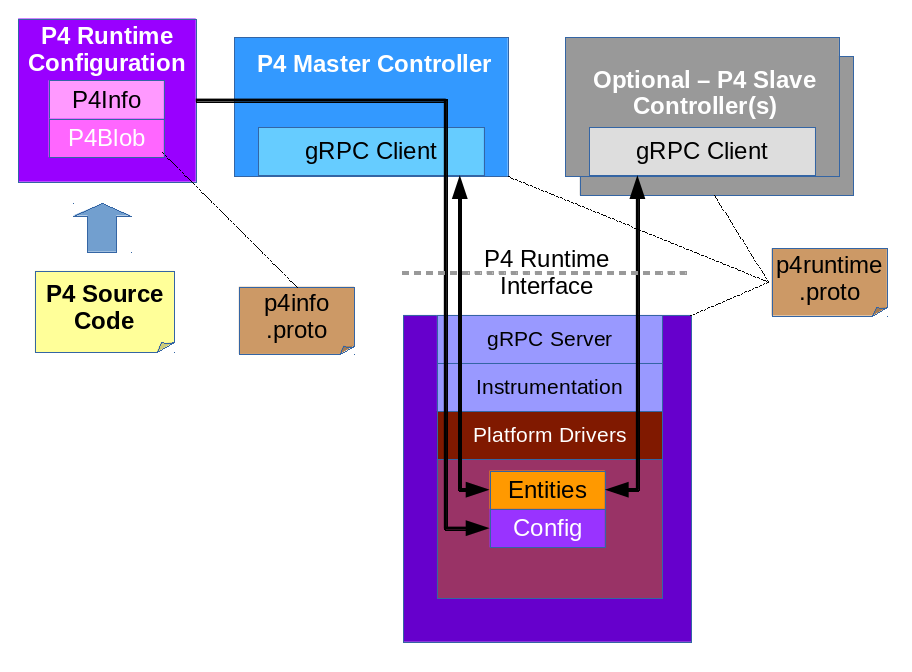
\includegraphics[keepaspectratio=true,height=7cm]{build/reference-architecture}{}\mdline{410}%mdk

%mdk-data-line={411}
\mdhr{}%mdk

%mdk-data-line={412}
\noindent\mdline{412}\mdcaption{\textbf{Figure~\mdcaptionlabel{1}.}~\mdcaptiontext{P4Runtime Reference Architecture.}}%mdk
%mdk
\end{mdcenter}\label{fig-reference-architecture}%mdk
%mdk
\end{figure}%mdk

%mdk-data-line={416}
\subsection{\mdline{416}3.1.\hspace*{0.5em}\mdline{416}Idealized Workflow}\label{sec-idealized-workflow}%mdk%mdk

%mdk-data-line={418}
\noindent\mdline{418}In the idealized workflow, a P4 source program is compiled to produce both a P4
device config and P4Info metadata. These comprise the \mdline{419}\mdcode{{\mdfontfamily{LuxiMono}{\mdfontsize{\dimfont{0.75}}ForwardingPipelineConfig}}}\mdline{419}
message. A P4Runtime controller chooses a configuration appropriate to a
particular target and installs it via a \mdline{421}\mdcode{{\mdfontfamily{LuxiMono}{\mdfontsize{\dimfont{0.75}}SetForwardingPipelineConfig}}}\mdline{421}
RPC. Metadata in the P4Info describes both the overall program itself
(\mdline{423}\mdcode{{\mdfontfamily{LuxiMono}{\mdfontsize{\dimfont{0.75}}PkgInfo}}}\mdline{423}) as well as all entity instances derived from the P4 program\mdline{423} \mdline{423}\textemdash{}\mdline{423}
tables and extern instances. Each entity instance has an associated numeric ID
assigned by the P4 compiler which serves as a concise \mdline{425}\textquotedblleft{}handle\textquotedblright{}\mdline{425} used in API
calls.%mdk

%mdk-data-line={428}
\mdline{428}In this workflow, P4 compiler backends are developed for each unique type of
target and produce P4Info and a target-specific device config. The P4Info schema
is designed to be target and architecture-independent, although the specific
contents are likely to be architecture-dependent. The compiler ensures the code
is compatible with the specific target and rejects code which is incompatible.%mdk

%mdk-data-line={434}
\mdline{434}In some use cases, it is expected that a controller will store a
collection of multiple P4 \mdline{435}\textquotedblleft{}packages\textquotedblright{}\mdline{435}, where each package consists of
the P4 device config and P4Info, and install them at will onto the target. A
controller can also query the \mdline{437}\mdcode{{\mdfontfamily{LuxiMono}{\mdfontsize{\dimfont{0.75}}ForwardingPipelineConfig}}}\mdline{437} from the target via the
\mdline{438}\mdcode{{\mdfontfamily{LuxiMono}{\mdfontsize{\dimfont{0.75}}GetForwardingPipelineRequest}}}\mdline{438} RPC. This can be useful to obtain the pipeline
configuration from a running device to synchronize the controller to its current
state.%mdk

%mdk-data-line={442}
\subsection{\mdline{442}3.2.\hspace*{0.5em}\mdline{442}P4 as a Behavioral Description Language}\label{sec-p4-as-behavioral-description-language}%mdk%mdk

%mdk-data-line={444}
\noindent\mdline{444}P4 can be considered a behavioral description of a switching device which may or
may not execute \mdline{445}\textquotedblleft{}P4\textquotedblright{}\mdline{445} natively. There is no requirement that a P4 compiler be
used in the production of either the P4 device config or the P4Info. There is no
absolute requirement that the target accept a \mdline{447}\mdcode{{\mdfontfamily{LuxiMono}{\mdfontsize{\dimfont{0.75}}SetForwardingPipelineRequest}}}\mdline{447} to
change its pipeline \mdline{448}\textquotedblleft{}program\textquotedblright{}\mdline{448}, as some devices may be fixed in function, or
configured via means other than P4 programs. Furthermore, a controller can run
without a P4 source program, since the P4Info file provides all of the
information necessary to describe the P4Runtime API messages needed to configure
such a device.%mdk

%mdk-data-line={454}
\mdline{454}While a P4 program does provide a precise description of the data plane
behavior, and this can prove invaluable in writing correct control plane
software, in some cases it is enough for a control plane software developer to
have the control plane API, plus good documentation of the data plane
behavior. Some device vendors may wish to keep their P4 source code private. The
minimum requirement for the controller and device to communicate properly is a
P4Info file that can be loaded by a controller in order to render the correct
P4Runtime API.%mdk

%mdk-data-line={463}
\mdline{463}In such scenarios, it is crucial to have detailed documentation, perhaps
included in the P4Info file itself, specifically the metadata in the \mdline{464}\mdcode{{\mdfontfamily{LuxiMono}{\mdfontsize{\dimfont{0.75}}PkgInfo}}}\mdline{464}
message as well as the embedded \mdline{465}\mdcode{{\mdfontfamily{LuxiMono}{\mdfontsize{\dimfont{0.75}}doc}}}\mdline{465} fields. Nevertheless, a P4 program which
describes the pipeline is ideally available. The contents of the P4Info file
will be described in later sections.%mdk

%mdk-data-line={469}
\subsection{\mdline{469}3.3.\hspace*{0.5em}\mdline{469}Alternative Workflows}\label{sec-alternative-workflows}%mdk%mdk

%mdk-data-line={471}
\noindent\mdline{471}Given the notions above concerning P4 code as behavioral description and P4Info
as API metadata, some other workflows are possible. The scenarios below are just
examples and actual situations may vary.%mdk

%mdk-data-line={475}
\subsubsection{\mdline{475}3.3.1.\hspace*{0.5em}\mdline{475}P4 Source Available, Compiled into P4Info but not Compiled into P4 Device Config}\label{sec-p4-source-available-compiled-into-p4info-but-not-compiled-into-p4-device-config}%mdk%mdk

%mdk-data-line={477}
\noindent\mdline{477}In this situation, P4 source code is available mainly as a behavioral model and
compiled to produce P4Info, but it is not compiled to produce the
\mdline{479}\mdcode{{\mdfontfamily{LuxiMono}{\mdfontsize{\dimfont{0.75}}p4\_device\_config}}}\mdline{479}. The device\mdline{479}'\mdline{479}s configuration might be derived via some other
means to implement the P4 source code\mdline{480}'\mdline{480}s intentions. The P4 code, if available,
can be studied to understand the pipeline, and the P4Info can be used to
implement the control plane.%mdk

%mdk-data-line={484}
\subsubsection{\mdline{484}3.3.2.\hspace*{0.5em}\mdline{484}No P4 Source Available, P4Info Available}\label{sec-no-p4-source-available-p4info-available}%mdk%mdk

%mdk-data-line={486}
\noindent\mdline{486}In this situation, P4Info is available but no P4 source is available for any
number of reasons, the most likely of which are:%mdk

%mdk-data-line={489}
\begin{enumerate}%mdk

%mdk-data-line={489}
\item{}
%mdk-data-line={489}
\mdline{489}The vendor or organization does not wish to divulge the P4 source code, to
protect intellectual property or maintain security.%mdk%mdk

%mdk-data-line={492}
\item{}
%mdk-data-line={492}
\mdline{492}The target was not implemented using P4 code to begin with, although it still
obeys the control plane API specified in the P4Info.%mdk%mdk
%mdk
\end{enumerate}%mdk

%mdk-data-line={495}
\noindent\mdline{495}As discussed in Section\mdline{495}~\mdref{sec-p4-as-behavioral-description-language}{3.2}\mdline{495}, in the
absence of a P4 program describing the data plane behavior, the detailed
knowledge required to write correct control plane code must come from other
sources, \mdline{498}e.g.\mdline{498} documentation.%mdk

%mdk-data-line={500}
\subsubsection{\mdline{500}3.3.3.\hspace*{0.5em}\mdline{500}Partial P4Info and P4 Source are Available}\label{sec-partial-p4info-and-p4-source-are-available}%mdk%mdk

%mdk-data-line={502}
\noindent\mdline{502}In this situation, a subset of the target\mdline{502}'\mdline{502}s pipeline configuration is exposed as
P4 source code and P4Info. The complete device behavior might be expressed as a
larger P4 program and P4Info, but these are not exposed to everybody. This
limits API access to only certain functions and behaviors. The hidden functions
and APIs might be available to select users who would have access to the
complete P4Info and possibly P4 source code.%mdk

%mdk-data-line={509}
\subsubsection{\mdline{509}3.3.4.\hspace*{0.5em}\mdline{509}P4Info Role-Based Subsets}\label{sec-p4info-role-based-subsets}%mdk%mdk

%mdk-data-line={511}
\noindent\mdline{511}In this situation, P4Info is selectively packaged into role-based subsets to
allow some controllers access to just the functionality required. For example, a
controller may only need read access to statistics counters and nothing more.%mdk

%mdk-data-line={515}
\subsection{\mdline{515}3.4.\hspace*{0.5em}\mdline{515}P4Runtime State Across Restarts}\label{sec-restarts}%mdk%mdk

%mdk-data-line={517}
\noindent\mdline{517}All targets support full restarts, where all forwarding state is reset and the
P4Runtime server starts with a clean state.  Some targets may also support
In-Service Software Upgrade (ISSU), where the software on the target can be
restarted while traffic is being forwarded. In this case, the P4Runtime server
may have the ability to access information from memory before the upgrade.%mdk

%mdk-data-line={523}
\section{\mdline{523}4.\hspace*{0.5em}\mdline{523}Controller Use-cases}\label{sec-controller-use-cases}%mdk%mdk

%mdk-data-line={525}
\noindent\mdline{525}P4Runtime allows for more than one controller. The mechanisms and semantics are
described in a later
\mdline{527}\mdref{sec-master-slave-arbitration-and-controller-replication}{section}\mdline{527}. Here we
present a number of use-cases. Each use-case highlights a particular aspect of
P4Runtime\mdline{529}'\mdline{529}s flexibility and is not intended to be exhaustive. Real-world
use-cases may combine various techniques and be more complex.%mdk

%mdk-data-line={532}
\subsection{\mdline{532}4.1.\hspace*{0.5em}\mdline{532}Single Embedded Controller}\label{sec-single-embedded-controller}%mdk%mdk

%mdk-data-line={534}
\noindent\mdline{534}Figure\mdline{534}~\mdref{fig-single-embedded-controller}{\mdcaptionlabel{2}}\mdline{534} shows perhaps the simplest use-case. A
device or target has an embedded controller which communicates to an on-board
switch via P4Runtime. This might be appropriate for an embedded appliance which
is not intended for SDN use-cases.%mdk

%mdk-data-line={539}
\mdline{539}P4Runtime was designed to be a viable embedded API. Complex controller
architectures typically feature multiple processes communicating with some sort
of IPC (Inter-Process Communications). P4Runtime is thus both an ideal RPC and
an IPC.%mdk

%mdk-data-line={544}
\begin{figure}[tbp]%mdk
\begin{mdcenter}%mdk

%mdk-data-line={545}
\noindent\mdline{545}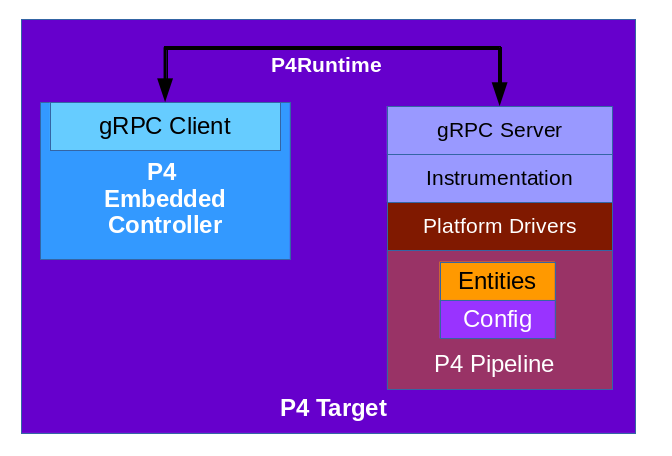
\includegraphics[keepaspectratio=true,height=6cm]{build/single-embedded-controller}{}\mdline{545}%mdk

%mdk-data-line={546}
\mdhr{}%mdk

%mdk-data-line={547}
\noindent\mdline{547}\mdcaption{\textbf{Figure~\mdcaptionlabel{2}.}~\mdcaptiontext{Use-Case: Single Embedded Controller}}%mdk
%mdk
\end{mdcenter}\label{fig-single-embedded-controller}%mdk
%mdk
\end{figure}%mdk

%mdk-data-line={551}
\subsection{\mdline{551}4.2.\hspace*{0.5em}\mdline{551}Single Remote Controller}\label{sec-single-remote-controller}%mdk%mdk

%mdk-data-line={553}
\noindent\mdline{553}Figure\mdline{553}~\mdref{fig-single-remote-controller}{\mdcaptionlabel{3}}\mdline{553} shows a single remote Controller in
charge of the P4 target. In this use-case, the device has no control of the
pipeline, it just hosts the server. While this is possible, it is probably more
practical to have a hybrid use-case as described in subsequent sections.%mdk

%mdk-data-line={558}
\begin{figure}[tbp]%mdk
\begin{mdcenter}%mdk

%mdk-data-line={559}
\noindent\mdline{559}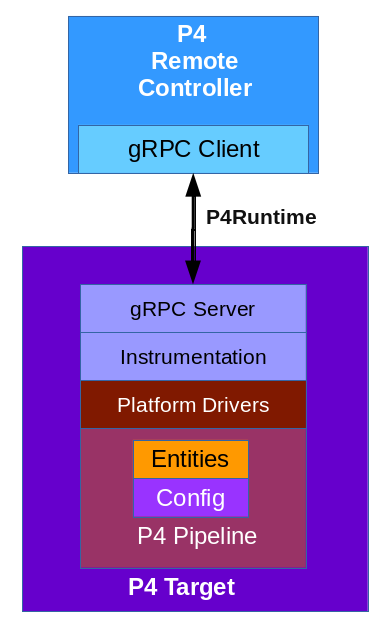
\includegraphics[keepaspectratio=true,height=7cm]{build/single-remote-controller}{}\mdline{559}%mdk

%mdk-data-line={560}
\mdhr{}%mdk

%mdk-data-line={561}
\noindent\mdline{561}\mdcaption{\textbf{Figure~\mdcaptionlabel{3}.}~\mdcaptiontext{Use-Case: Single Remote Controller}}%mdk
%mdk
\end{mdcenter}\label{fig-single-remote-controller}%mdk
%mdk
\end{figure}%mdk

%mdk-data-line={565}
\subsection{\mdline{565}4.3.\hspace*{0.5em}\mdline{565}Embedded\mdline{565} \mdline{565}+ Single Remote Controller}\label{sec-embedded-single-remote-controller}%mdk%mdk

%mdk-data-line={567}
\noindent\mdline{567}Figure\mdline{567}~\mdref{fig-embedded-plus-single-remote-controller}{\mdcaptionlabel{4}}\mdline{567} illustrates the use-case of
an embedded controller plus a single remote controller. Both controllers are
clients of the single server. The embedded controller is in charge of one set of
P4 entities plus the pipeline configuration. The remote controller is in charge
of the remainder of the P4 entities. An equally-valid, alternative use-case,
could assign the pipeline configuration to the remote controller.%mdk

%mdk-data-line={574}
\mdline{574}For example, to minimize round-trip times (RTT) it might make sense for the
embedded controller to manage the contents of a fast-failover table. The remote
controller might manage the contents of routing tables.%mdk

%mdk-data-line={578}
\begin{figure}[tbp]%mdk
\begin{mdcenter}%mdk

%mdk-data-line={579}
\noindent\mdline{579}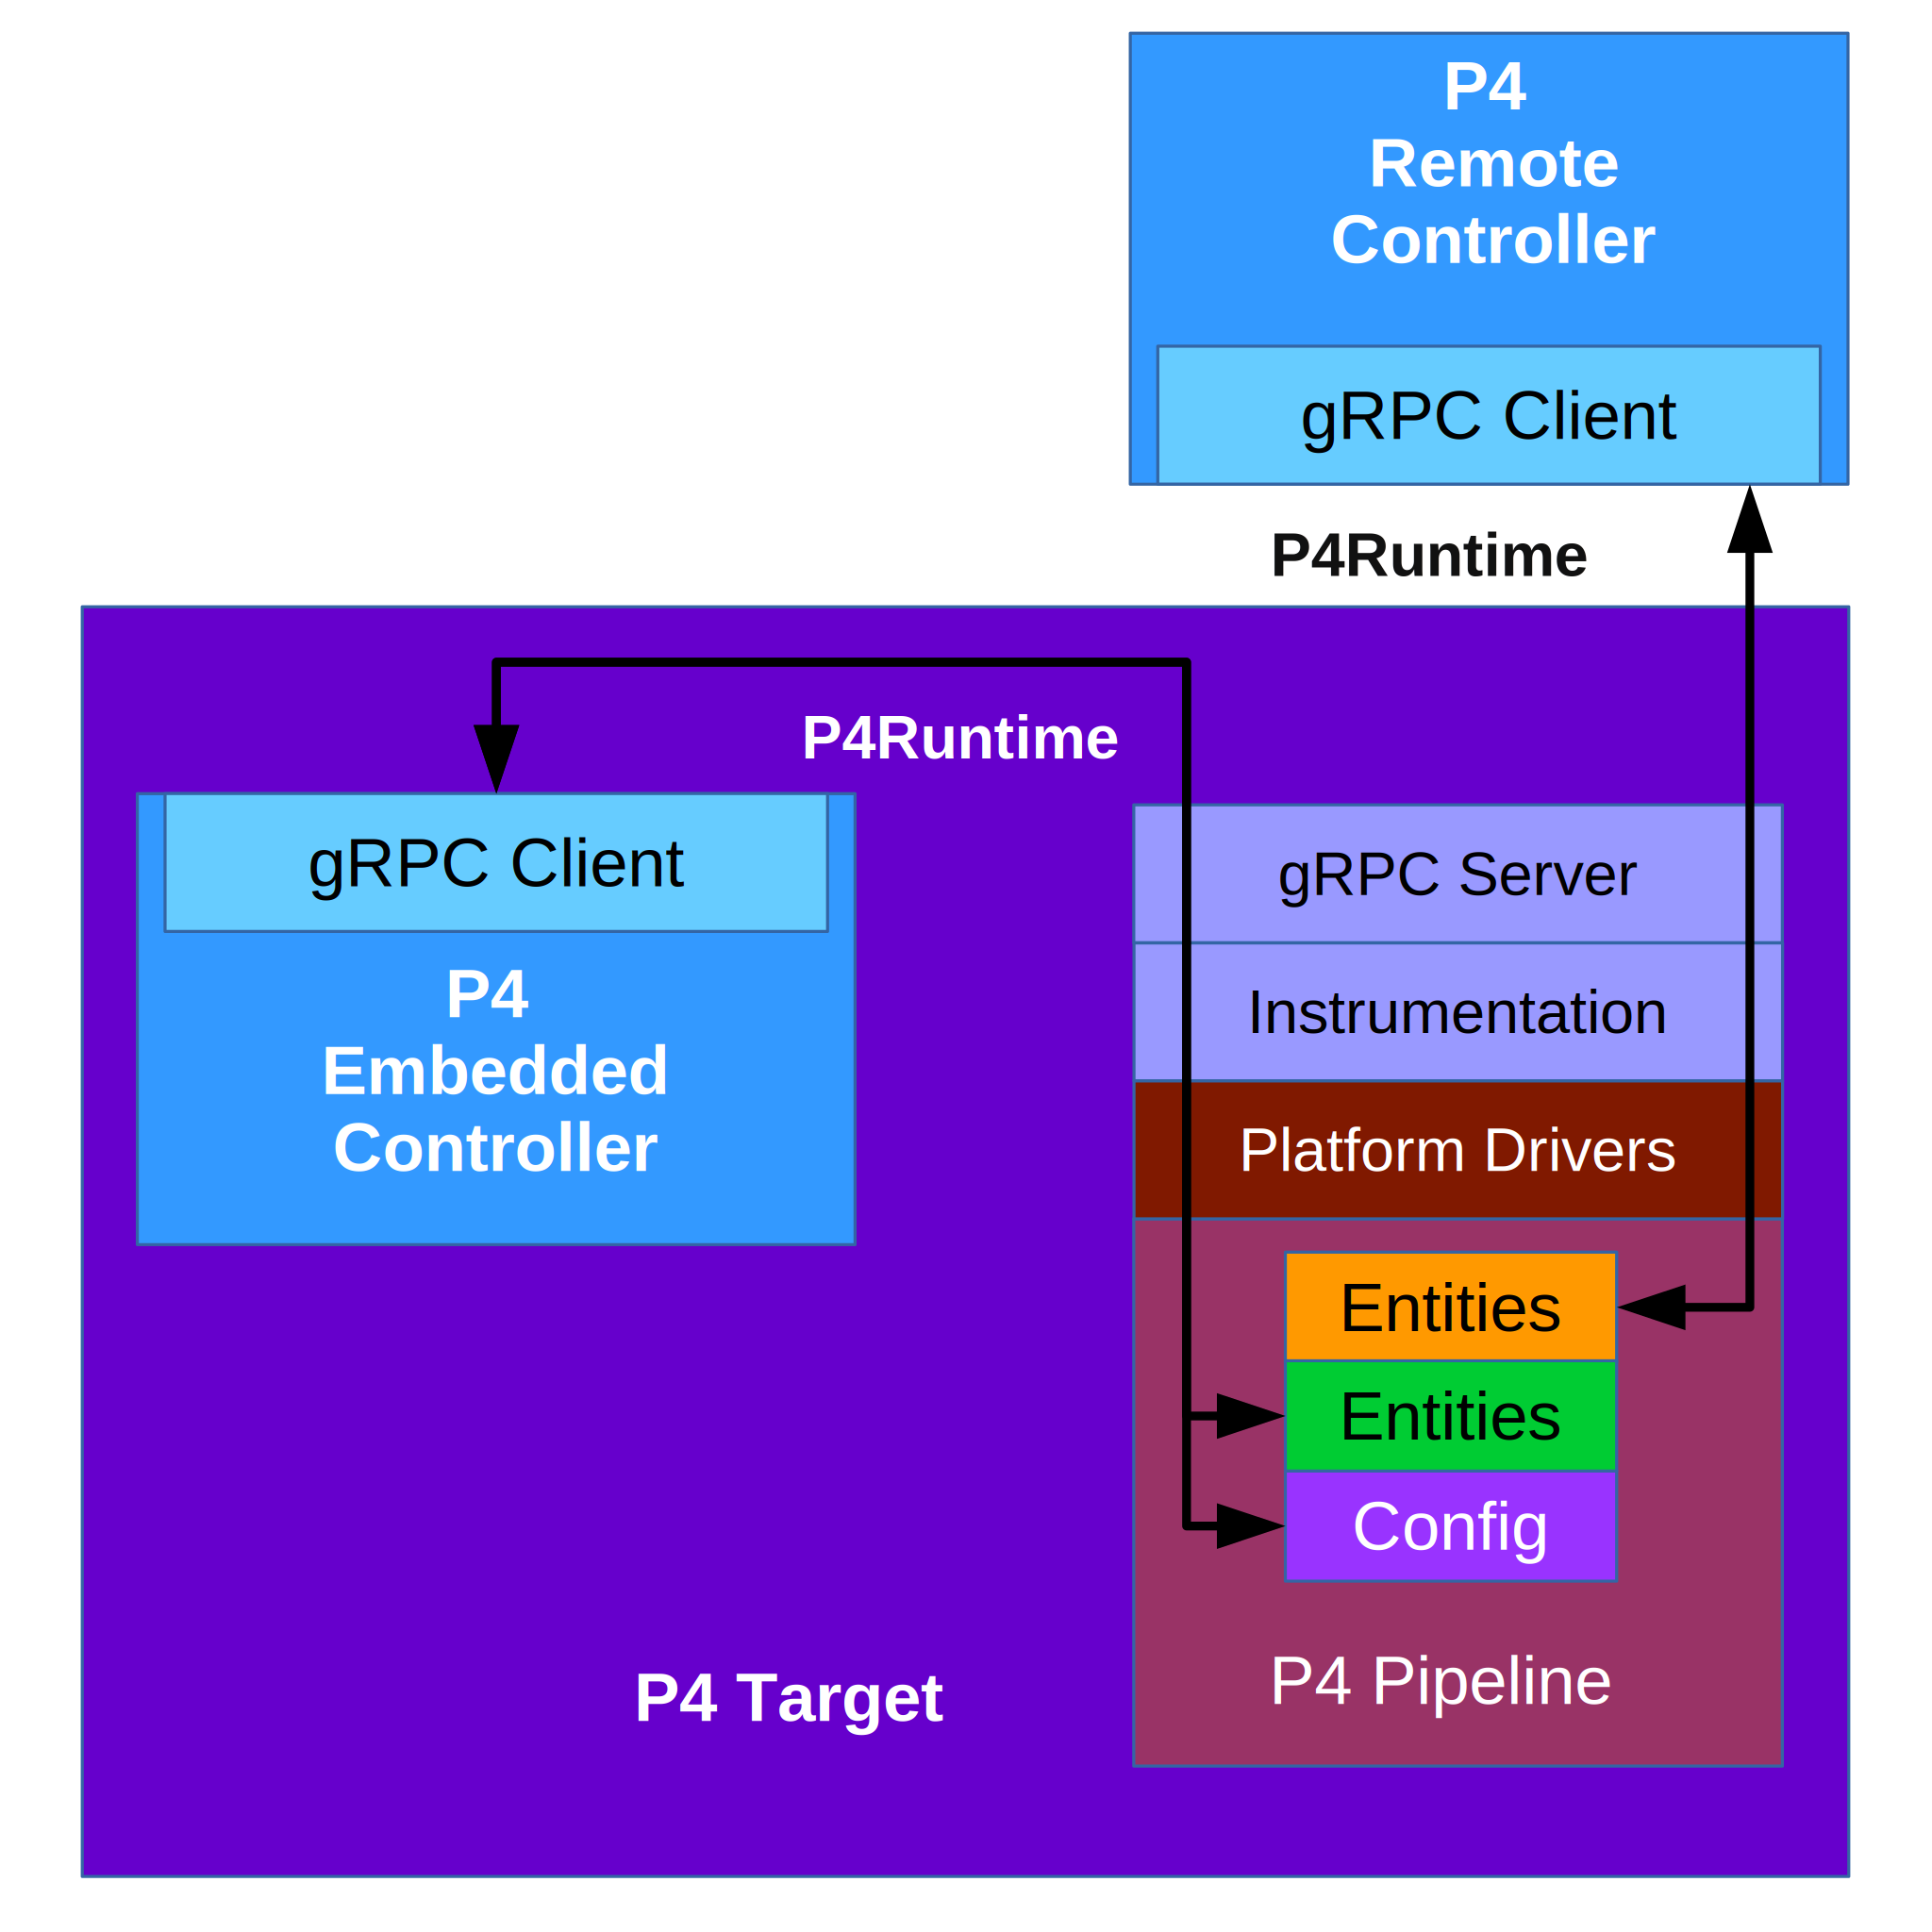
\includegraphics[keepaspectratio=true,height=7cm]{build/embedded-plus-single-remote-controller}{}\mdline{579}%mdk

%mdk-data-line={580}
\mdhr{}%mdk

%mdk-data-line={581}
\noindent\mdline{581}\mdcaption{\textbf{Figure~\mdcaptionlabel{4}.}~\mdcaptiontext{Use-Case: Embedded Plus Single Remote Controller}}%mdk
%mdk
\end{mdcenter}\label{fig-embedded-plus-single-remote-controller}%mdk
%mdk
\end{figure}%mdk

%mdk-data-line={586}
\subsection{\mdline{586}4.4.\hspace*{0.5em}\mdline{586}Embedded\mdline{586} \mdline{586}+ Two Remote Controllers}\label{sec-embedded-two-remote-controllers}%mdk%mdk

%mdk-data-line={588}
\noindent\mdline{588}Figure\mdline{588}~\mdref{fig-embedded-plus-two-remote-controllers}{\mdcaptionlabel{5}}\mdline{588} illustrates the case of an
embedded controller similar to the previous use-case, and two remote
controllers. One of the remote controllers is responsible for some entities,
\mdline{591}e.g.\mdline{591} routing tables, and the other remote controller is responsible for other
entities, perhaps statistics tables. Role-based access divides the ownership.%mdk

%mdk-data-line={594}
\begin{figure}[tbp]%mdk
\begin{mdcenter}%mdk

%mdk-data-line={595}
\noindent\mdline{595}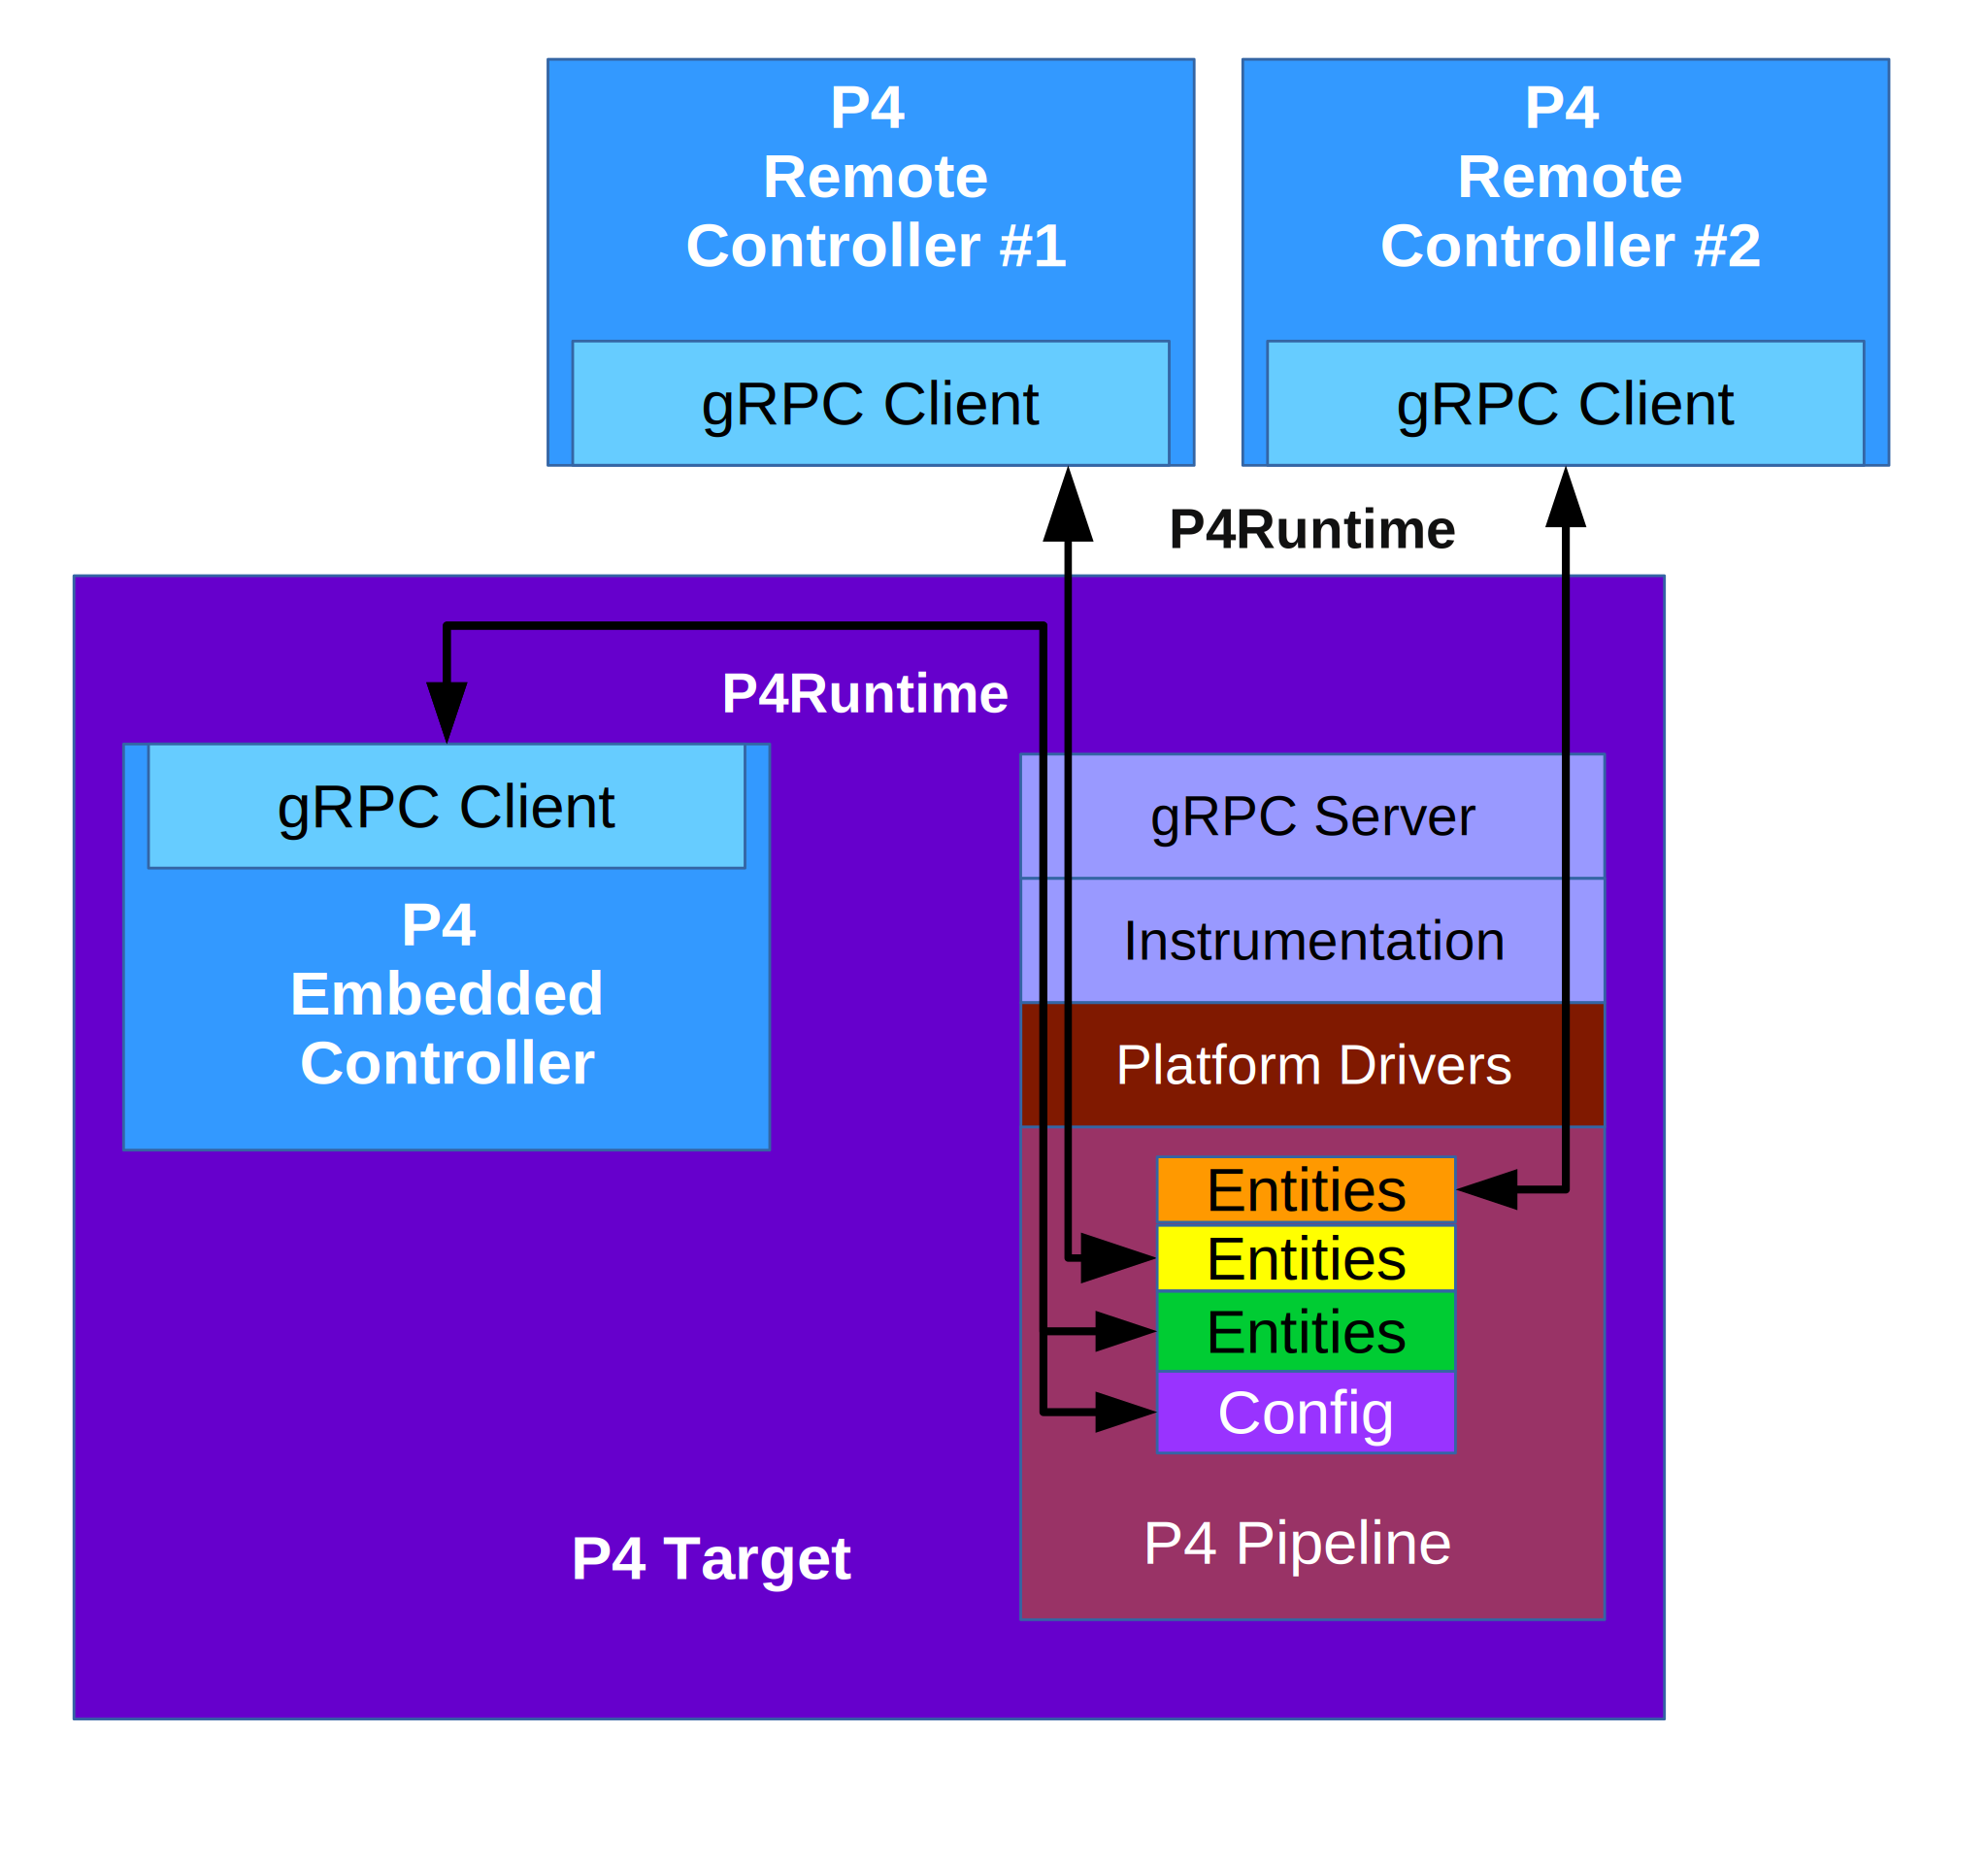
\includegraphics[keepaspectratio=true,height=7cm]{build/embedded-plus-two-remote-controllers}{}\mdline{595}%mdk

%mdk-data-line={596}
\mdhr{}%mdk

%mdk-data-line={597}
\noindent\mdline{597}\mdcaption{\textbf{Figure~\mdcaptionlabel{5}.}~\mdcaptiontext{Use-Case: Embedded Plus Two Remote Controllers}}%mdk
%mdk
\end{mdcenter}\label{fig-embedded-plus-two-remote-controllers}%mdk
%mdk
\end{figure}%mdk

%mdk-data-line={602}
\subsection{\mdline{602}4.5.\hspace*{0.5em}\mdline{602}Embedded Controller\mdline{602} \mdline{602}+ Two High-Availability Remote Controllers}\label{sec-embedded-controller-two-high-availability-remote-controllers}%mdk%mdk

%mdk-data-line={604}
\noindent\mdline{604}Figure\mdline{604}~\mdref{fig-embedded-plus-two-remote-ha-controllers}{\mdcaptionlabel{6}}\mdline{604} illustrates a single
embedded controller plus two remote controllers in an active-standby HA
(High-Availability) configuration. Controller \mdline{606}\#\mdline{606}1 is the active controller and is
in charge of some entities. If it fails, Controller \mdline{607}\#\mdline{607}2 takes over and manages
the tables formerly owned by Controller \mdline{608}\#\mdline{608}1. The mechanics of HA architectures
are beyond the scope of this document, but the P4Runtime multi-master
arbitration scheme supports it.%mdk

%mdk-data-line={612}
\begin{figure}[tbp]%mdk
\begin{mdcenter}%mdk

%mdk-data-line={613}
\noindent\mdline{613}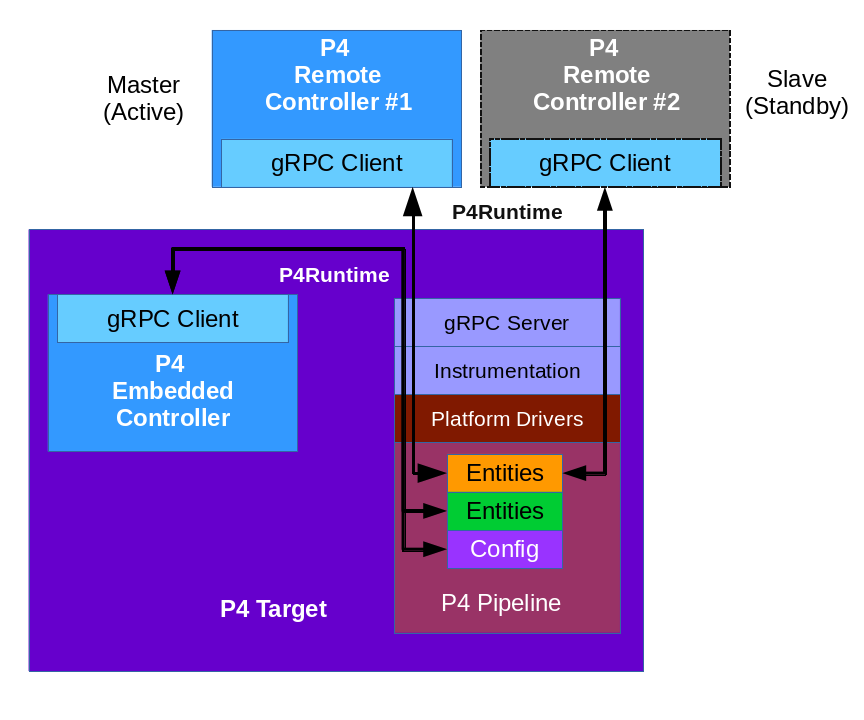
\includegraphics[keepaspectratio=true,height=7cm]{build/embedded-plus-two-remote-ha-controllers}{}\mdline{613}%mdk

%mdk-data-line={614}
\mdhr{}%mdk

%mdk-data-line={615}
\noindent\mdline{615}\mdcaption{\textbf{Figure~\mdcaptionlabel{6}.}~\mdcaptiontext{Use-Case: Embedded Plus Two Remote High-Availability Controllers}}%mdk
%mdk
\end{mdcenter}\label{fig-embedded-plus-two-remote-ha-controllers}%mdk
%mdk
\end{figure}%mdk

%mdk-data-line={620}
\section{\mdline{620}5.\hspace*{0.5em}\mdline{620}Master-Slave Arbitration and Controller Replication}\label{sec-master-slave-arbitration-and-controller-replication}%mdk%mdk

%mdk-data-line={623}
\noindent\mdline{623}The P4Runtime interface allows multiple controllers to be connected to the
P4Runtime server running on the device at the same time for the following
reasons:%mdk

%mdk-data-line={627}
\begin{enumerate}%mdk

%mdk-data-line={627}
\item{}
%mdk-data-line={627}
\mdline{627}Partitioning of the control plane: Multiple controllers may have orthogonal,
non-overlapping, \mdline{628}\textquotedblleft{}roles\textquotedblright{}\mdline{628} (or \mdline{628}\textquotedblleft{}realms\textquotedblright{}\mdline{628}) and should be able to push forwarding
entities simultaneously. The control plane can be partitioned into multiple
roles and each role will have a set of controllers, one of which is the
master and the rest are slaves. Role definition, \mdline{631}i.e.\mdline{631} how P4 entities get
assigned to each role, is \mdline{632}\textbf{out-of-scope}\mdline{632} of this document.%mdk%mdk

%mdk-data-line={634}
\item{}
%mdk-data-line={634}
\mdline{634}Redundancy and fault tolerance: Supporting multiple controllers allows having
one or more standby slave controllers. These can already have a connection
open, which can help them become master more quickly, especially in the case
where the control-plane traffic is in-band and connection setup might be more
involved.%mdk%mdk
%mdk
\end{enumerate}%mdk

%mdk-data-line={640}
\noindent\mdline{640}To support multiple controllers, P4Runtime uses the streaming channel (available
via \mdline{641}\mdcode{{\mdfontfamily{LuxiMono}{\mdfontsize{\dimfont{0.75}}StreamChannel}}}\mdline{641} RPC) for session management. The workflow is described as
follows:%mdk

%mdk-data-line={644}
\begin{itemize}%mdk

%mdk-data-line={644}
\item{}
%mdk-data-line={644}
\mdline{644}Each controller instance (\mdline{644}e.g.\mdline{644} a controller process) can participate in one or
more roles. For each (\mdline{645}\mdcode{{\mdfontfamily{LuxiMono}{\mdfontsize{\dimfont{0.75}}device\_id}}}\mdline{645}, \mdline{645}\mdcode{{\mdfontfamily{LuxiMono}{\mdfontsize{\dimfont{0.75}}role\_id}}}\mdline{645}), the controller receives an
\mdline{646}\mdcode{{\mdfontfamily{LuxiMono}{\mdfontsize{\dimfont{0.75}}election\_id}}}\mdline{646}. This \mdline{646}\mdcode{{\mdfontfamily{LuxiMono}{\mdfontsize{\dimfont{0.75}}election\_id}}}\mdline{646} can be the same for different roles and/or
devices, as long as the tuple (\mdline{647}\mdcode{{\mdfontfamily{LuxiMono}{\mdfontsize{\dimfont{0.75}}device\_id}}}\mdline{647}, \mdline{647}\mdcode{{\mdfontfamily{LuxiMono}{\mdfontsize{\dimfont{0.75}}role\_id}}}\mdline{647}, \mdline{647}\mdcode{{\mdfontfamily{LuxiMono}{\mdfontsize{\dimfont{0.75}}election\_id}}}\mdline{647}) is
unique. For each (\mdline{648}\mdcode{{\mdfontfamily{LuxiMono}{\mdfontsize{\dimfont{0.75}}device\_id}}}\mdline{648}, \mdline{648}\mdcode{{\mdfontfamily{LuxiMono}{\mdfontsize{\dimfont{0.75}}role\_id}}}\mdline{648}) that the controller wishes to
control, it establishes a \mdline{649}\mdcode{{\mdfontfamily{LuxiMono}{\mdfontsize{\dimfont{0.75}}StreamChannel}}}\mdline{649} with the P4Runtime server
responsible for that device, and sends a \mdline{650}\mdcode{{\mdfontfamily{LuxiMono}{\mdfontsize{\dimfont{0.75}}MasterArbitrationUpdate}}}\mdline{650} message
containing that tuple of (\mdline{651}\mdcode{{\mdfontfamily{LuxiMono}{\mdfontsize{\dimfont{0.75}}device\_id}}}\mdline{651}, \mdline{651}\mdcode{{\mdfontfamily{LuxiMono}{\mdfontsize{\dimfont{0.75}}role\_id}}}\mdline{651}, \mdline{651}\mdcode{{\mdfontfamily{LuxiMono}{\mdfontsize{\dimfont{0.75}}election\_id}}}\mdline{651}) values. The
P4Runtime server selects a master independently for each (\mdline{652}\mdcode{{\mdfontfamily{LuxiMono}{\mdfontsize{\dimfont{0.75}}device\_id}}}\mdline{652},
\mdline{653}\mdcode{{\mdfontfamily{LuxiMono}{\mdfontsize{\dimfont{0.75}}role\_id}}}\mdline{653}) pair. The master is the client that has the highest \mdline{653}\mdcode{{\mdfontfamily{LuxiMono}{\mdfontsize{\dimfont{0.75}}election\_id}}}\mdline{653}
that the device has ever received for the same (\mdline{654}\mdcode{{\mdfontfamily{LuxiMono}{\mdfontsize{\dimfont{0.75}}device\_id}}}\mdline{654},
\mdline{655}\mdcode{{\mdfontfamily{LuxiMono}{\mdfontsize{\dimfont{0.75}}role\_id}}}\mdline{655}) values.  A connection between a controller instance and a device id
\mdline{656}\textemdash{}\mdline{656} which involves a persistent \mdline{656}\mdcode{{\mdfontfamily{LuxiMono}{\mdfontsize{\dimfont{0.75}}StreamChannel}}}\mdline{656} \mdline{656}\textemdash{}\mdline{656} can be referred to as a
P4Runtime client.%mdk

%mdk-data-line={659}
\mdline{659}Note that the P4Runtime server does not assign a \mdline{659}\mdcode{{\mdfontfamily{LuxiMono}{\mdfontsize{\dimfont{0.75}}role\_id}}}\mdline{659} or \mdline{659}\mdcode{{\mdfontfamily{LuxiMono}{\mdfontsize{\dimfont{0.75}}election\_id}}}\mdline{659} to
any controller. It is up to an arbitration mechanism outside of the server to
decide on the controller roles, and the \mdline{661}\mdcode{{\mdfontfamily{LuxiMono}{\mdfontsize{\dimfont{0.75}}election\_id}}}\mdline{661} values used for each
\mdline{662}\mdcode{{\mdfontfamily{LuxiMono}{\mdfontsize{\dimfont{0.75}}StreamChannel}}}\mdline{662}. The P4Runtime server only keeps track of the (\mdline{662}\mdcode{{\mdfontfamily{LuxiMono}{\mdfontsize{\dimfont{0.75}}device\_id}}}\mdline{662},
\mdline{663}\mdcode{{\mdfontfamily{LuxiMono}{\mdfontsize{\dimfont{0.75}}role\_id}}}\mdline{663}, \mdline{663}\mdcode{{\mdfontfamily{LuxiMono}{\mdfontsize{\dimfont{0.75}}election\_id}}}\mdline{663}) of each \mdline{663}\mdcode{{\mdfontfamily{LuxiMono}{\mdfontsize{\dimfont{0.75}}StreamChannel}}}\mdline{663} that has sent a successful
\mdline{664}\mdcode{{\mdfontfamily{LuxiMono}{\mdfontsize{\dimfont{0.75}}MasterArbitrationUpdate}}}\mdline{664} message, and maintains the invariant that all such
3-tuples are unique. A server must use all three of these values from a
\mdline{666}\mdcode{{\mdfontfamily{LuxiMono}{\mdfontsize{\dimfont{0.75}}WriteRequest}}}\mdline{666} message to identify which client is making the \mdline{666}\mdcode{{\mdfontfamily{LuxiMono}{\mdfontsize{\dimfont{0.75}}WriteRequest}}}\mdline{666},
not only the \mdline{667}\mdcode{{\mdfontfamily{LuxiMono}{\mdfontsize{\dimfont{0.75}}election\_id}}}\mdline{667}. This enables controllers to re-use the same
numeric \mdline{668}\mdcode{{\mdfontfamily{LuxiMono}{\mdfontsize{\dimfont{0.75}}election\_id}}}\mdline{668} values across different (\mdline{668}\mdcode{{\mdfontfamily{LuxiMono}{\mdfontsize{\dimfont{0.75}}device\_id}}}\mdline{668}, \mdline{668}\mdcode{{\mdfontfamily{LuxiMono}{\mdfontsize{\dimfont{0.75}}role\_id}}}\mdline{668})
pairs. P4Runtime does not require \mdline{669}\mdcode{{\mdfontfamily{LuxiMono}{\mdfontsize{\dimfont{0.75}}election\_id}}}\mdline{669} values be reused across such
different (\mdline{670}\mdcode{{\mdfontfamily{LuxiMono}{\mdfontsize{\dimfont{0.75}}device\_id}}}\mdline{670}, \mdline{670}\mdcode{{\mdfontfamily{LuxiMono}{\mdfontsize{\dimfont{0.75}}role\_id}}}\mdline{670}) pairs; it allows it.%mdk%mdk

%mdk-data-line={672}
\item{}
%mdk-data-line={672}
\mdline{672}To start a controller session, a controller first opens a bidirectional stream
channel to the server via the \mdline{673}\mdcode{{\mdfontfamily{LuxiMono}{\mdfontsize{\dimfont{0.75}}StreamChannel}}}\mdline{673} RPC for each device. This stream
will be used for two purposes:%mdk

%mdk-data-line={676}
\begin{itemize}%mdk

%mdk-data-line={676}
\item{}
%mdk-data-line={676}
\mdline{676}\textbf{Session management:}\mdline{676} As soon as the controller opens the stream
channel, it sends a \mdline{677}\mdcode{{\mdfontfamily{LuxiMono}{\mdfontsize{\dimfont{0.75}}StreamMessageRequest}}}\mdline{677} message to the switch. The
controller populates the \mdline{678}\mdcode{{\mdfontfamily{LuxiMono}{\mdfontsize{\dimfont{0.75}}MasterArbitrationUpdate}}}\mdline{678} field in this message
using its \mdline{679}\mdcode{{\mdfontfamily{LuxiMono}{\mdfontsize{\dimfont{0.75}}role\_id}}}\mdline{679} and \mdline{679}\mdcode{{\mdfontfamily{LuxiMono}{\mdfontsize{\dimfont{0.75}}election\_id}}}\mdline{679}, as well as the \mdline{679}\mdcode{{\mdfontfamily{LuxiMono}{\mdfontsize{\dimfont{0.75}}device\_id}}}\mdline{679} of the
device. Note that the \mdline{680}\mdcode{{\mdfontfamily{LuxiMono}{\mdfontsize{\dimfont{0.75}}status}}}\mdline{680} field in the \mdline{680}\mdcode{{\mdfontfamily{LuxiMono}{\mdfontsize{\dimfont{0.75}}MasterArbitrationUpdate}}}\mdline{680} is
not populated by the controller. This field is populated by the P4Runtime
server when it sends a response back to the client, as explained below.%mdk%mdk

%mdk-data-line={684}
\item{}
%mdk-data-line={684}
\mdline{684}\textbf{Streaming of notifications (e.g. digests) and packet I/O:}\mdline{684} The same
streaming channel will be used for streaming notifications, as well as for
packet-in and packet-out messages. Note that unless specified otherwise by
the role definitions, only the master controller can participate in packet
I/O. This feature is explained in more details in the\mdline{688}~\mdref{sec-packet-i_o}{Packet
I/O}\mdline{689} section.%mdk%mdk
%mdk
\end{itemize}%mdk

%mdk-data-line={691}
\mdline{691}Note that a controller session is only required if the controller wants to do
Packet I/O, or modify the forwarding state.%mdk%mdk

%mdk-data-line={694}
\item{}
%mdk-data-line={694}
\mdline{694}Note that the stream is opened per device. In case a switching platform has
multiple devices (\mdline{695}e.g.\mdline{695} multi-ASIC line card) which are all controlled via the
same P4Runtime server, it is possible to have different masters for different
devices. In this case, it is the responsibility of the P4Runtime server to
keep track of the master for each device (and role). More specifically, the
P4Runtime server will know which stream corresponds to the master controller
for each pair of (\mdline{700}\mdcode{{\mdfontfamily{LuxiMono}{\mdfontsize{\dimfont{0.75}}device\_id}}}\mdline{700}, \mdline{700}\mdcode{{\mdfontfamily{LuxiMono}{\mdfontsize{\dimfont{0.75}}role\_id}}}\mdline{700}) at any point of time.%mdk%mdk

%mdk-data-line={702}
\item{}
%mdk-data-line={702}
\mdline{702}The streaming channel between the controller and the server defines the
liveness of the controller session. The controller is considered \mdline{703}\textquotedblleft{}offline\textquotedblright{}\mdline{703} or
\mdline{704}\textquotedblleft{}dead\textquotedblright{}\mdline{704} as soon as its stream channel to the switch is broken. When a master
channel gets broken: (i) an advisory message is sent to all other controllers
for that \mdline{706}\mdcode{{\mdfontfamily{LuxiMono}{\mdfontsize{\dimfont{0.75}}device\_id}}}\mdline{706} and \mdline{706}\mdcode{{\mdfontfamily{LuxiMono}{\mdfontsize{\dimfont{0.75}}role\_id}}}\mdline{706}, as described in the
\mdline{707}\mdref{sec-mastership-notification}{following section}\mdline{707} (ii) the P4Runtime server
will be without a master, until a client sends a successful
\mdline{709}\mdcode{{\mdfontfamily{LuxiMono}{\mdfontsize{\dimfont{0.75}}MasterArbitrationUpdate}}}\mdline{709} (as per the rules in a
\mdline{710}\mdref{sec-mastership-updates}{later section}\mdline{710}).%mdk%mdk

%mdk-data-line={712}
\item{}
%mdk-data-line={712}
\mdline{712}The mechanism via which the controller receives the P4Runtime server details
which includes the \mdline{713}\mdcode{{\mdfontfamily{LuxiMono}{\mdfontsize{\dimfont{0.75}}device\_id}}}\mdline{713}, \mdline{713}\mdcode{{\mdfontfamily{LuxiMono}{\mdfontsize{\dimfont{0.75}}ip}}}\mdline{713} and \mdline{713}\mdcode{{\mdfontfamily{LuxiMono}{\mdfontsize{\dimfont{0.75}}port}}}\mdline{713}, as well as the mechanism via
which it receives the Forwarding Pipeline Config, are implementation specific
and beyond the scope of this specification. Similarly, the mechanism via which
the P4Runtime server receives its switch config (which notably includes the
\mdline{717}\mdcode{{\mdfontfamily{LuxiMono}{\mdfontsize{\dimfont{0.75}}device\_id}}}\mdline{717}) is beyond the scope of this specification.  Nevertheless, if the
server details or switch config are transferred via the network, it is
recommended to use TLS or similar encryption and authentication mechanisms to
prevent eavesdropping attacks.%mdk%mdk
%mdk
\end{itemize}%mdk

%mdk-data-line={722}
\noindent\mdline{722}gRPC enables the server to identify which client originated each message in the
\mdline{723}\mdcode{{\mdfontfamily{LuxiMono}{\mdfontsize{\dimfont{0.75}}StreamChannel}}}\mdline{723} stream. For example, the C++ gRPC library\mdline{723}~[\mdcite{grpcstreamc}{10}]\mdline{723} in
synchronous mode enables a server process to cause a function to be called when
a new client creates a \mdline{725}\mdcode{{\mdfontfamily{LuxiMono}{\mdfontsize{\dimfont{0.75}}StreamChannel}}}\mdline{725} stream. This function should not return
until the stream is closed and the server has done any cleanup required when a
\mdline{727}\mdcode{{\mdfontfamily{LuxiMono}{\mdfontsize{\dimfont{0.75}}StreamChannel}}}\mdline{727} is closed normally (or broken, \mdline{727}e.g.\mdline{727} because a client process
unexpectedly terminated). Thus the server can easily associate all
\mdline{729}\mdcode{{\mdfontfamily{LuxiMono}{\mdfontsize{\dimfont{0.75}}StreamChannel}}}\mdline{729} messages received from the same client, because they are
processed within the context of the same function call.%mdk

%mdk-data-line={732}
\mdline{732}A P4Runtime implementation need not rely on the gRPC library providing
information with unary RPC messages that identify which client they came from.
Unary RPC messages include requests to write table entries in the data plane, or
read state from the data plane, among others described later. P4Runtime relies
on clients identifying themselves in every write request, by including the
values \mdline{737}\mdcode{{\mdfontfamily{LuxiMono}{\mdfontsize{\dimfont{0.75}}device\_id}}}\mdline{737}, \mdline{737}\mdcode{{\mdfontfamily{LuxiMono}{\mdfontsize{\dimfont{0.75}}role\_id}}}\mdline{737}, and \mdline{737}\mdcode{{\mdfontfamily{LuxiMono}{\mdfontsize{\dimfont{0.75}}election\_id}}}\mdline{737} in all write requests. The
server trusts clients not to use a triple of values other than their own in
their write requests. gRPC provides authentication methods\mdline{739}~[\mdcite{grpcauth}{8}]\mdline{739} that
should be deployed to prevent untrusted clients from creating channels, and thus
from making changes or even reading the state of the server.%mdk

%mdk-data-line={743}
\subsection{\mdline{743}5.1.\hspace*{0.5em}\mdline{743}Default Role}\label{sec-default-role}%mdk%mdk

%mdk-data-line={745}
\noindent\mdline{745}A controller can omit the role message in \mdline{745}\mdcode{{\mdfontfamily{LuxiMono}{\mdfontsize{\dimfont{0.75}}MasterArbitrationUpdate}}}\mdline{745}. This
implies the \mdline{746}\textquotedblleft{}default role\textquotedblright{}\mdline{746}, which corresponds to \mdline{746}\textquotedblleft{}full pipeline access\textquotedblright{}\mdline{746}. This
also implies that a default role has a \mdline{747}\mdcode{{\mdfontfamily{LuxiMono}{\mdfontsize{\dimfont{0.75}}role.id}}}\mdline{747} of 0 (default). If using a
default role, all RPCs from the controller (\mdline{748}e.g.\mdline{748} \mdline{748}\mdcode{{\mdfontfamily{LuxiMono}{\mdfontsize{\dimfont{0.75}}Write}}}\mdline{748}) must set the \mdline{748}\mdcode{{\mdfontfamily{LuxiMono}{\mdfontsize{\dimfont{0.75}}role\_id}}}\mdline{748}
to 0.%mdk

%mdk-data-line={751}
\subsection{\mdline{751}5.2.\hspace*{0.5em}\mdline{751}Role Config}\label{sec-arbitration-role-config}%mdk%mdk

%mdk-data-line={753}
\noindent\mdline{753}The \mdline{753}\mdcode{{\mdfontfamily{LuxiMono}{\mdfontsize{\dimfont{0.75}}role.config}}}\mdline{753} field in the \mdline{753}\mdcode{{\mdfontfamily{LuxiMono}{\mdfontsize{\dimfont{0.75}}MasterArbitrationUpdate}}}\mdline{753} message sent by the
controller describes the role configuration, \mdline{754}i.e.\mdline{754} which operations are in the
scope of a given role. In particular, the definition of a role may include the
following:%mdk

%mdk-data-line={758}
\begin{itemize}[noitemsep,topsep=\mdcompacttopsep]%mdk

%mdk-data-line={758}
\item\mdline{758}A list of P4 entities for which the controller may issue \mdline{758}\mdcode{{\mdfontfamily{LuxiMono}{\mdfontsize{\dimfont{0.75}}Write}}}\mdline{758} updates and
receive notification messages (\mdline{759}e.g.\mdline{759} \mdline{759}\mdcode{{\mdfontfamily{LuxiMono}{\mdfontsize{\dimfont{0.75}}DigestList}}}\mdline{759} and
\mdline{760}\mdcode{{\mdfontfamily{LuxiMono}{\mdfontsize{\dimfont{0.75}}IdleTimeoutNotification}}}\mdline{760}).%mdk

%mdk-data-line={761}
\item\mdline{761}Whether the controller is able to receive \mdline{761}\mdcode{{\mdfontfamily{LuxiMono}{\mdfontsize{\dimfont{0.75}}PacketIn}}}\mdline{761} messages, along with a
filtering mechanism based on the values of the \mdline{762}\mdcode{{\mdfontfamily{LuxiMono}{\mdfontsize{\dimfont{0.75}}PacketMetadata}}}\mdline{762} fields to
select which \mdline{763}\mdcode{{\mdfontfamily{LuxiMono}{\mdfontsize{\dimfont{0.75}}PacketIn}}}\mdline{763} messages should be sent to the controller.%mdk

%mdk-data-line={764}
\item\mdline{764}Whether the controller is able to send \mdline{764}\mdcode{{\mdfontfamily{LuxiMono}{\mdfontsize{\dimfont{0.75}}PacketOut}}}\mdline{764} messages, along with a
filtering mechanism based on the values of the \mdline{765}\mdcode{{\mdfontfamily{LuxiMono}{\mdfontsize{\dimfont{0.75}}PacketMetadata}}}\mdline{765} fields to
select which \mdline{766}\mdcode{{\mdfontfamily{LuxiMono}{\mdfontsize{\dimfont{0.75}}PacketOut}}}\mdline{766} messages are allowed to be sent by the controller.%mdk
%mdk
\end{itemize}%mdk

%mdk-data-line={768}
\noindent\mdline{768}An unset \mdline{768}\mdcode{{\mdfontfamily{LuxiMono}{\mdfontsize{\dimfont{0.75}}role.config}}}\mdline{768} implies \mdline{768}\textquotedblleft{}full pipeline access\textquotedblright{}\mdline{768} (similar to the default
role explained above). In order to support different role definition schemes,
\mdline{770}\mdcode{{\mdfontfamily{LuxiMono}{\mdfontsize{\dimfont{0.75}}role.config}}}\mdline{770} is defined as an \mdline{770}\mdcode{{\mdfontfamily{LuxiMono}{\mdfontsize{\dimfont{0.75}}Any}}}\mdline{770} Protobuf message\mdline{770}~[\mdcite{protoany}{29}]\mdline{770}. Such schemes
are out-of-scope of this document. When partitioning of the control plane is
desired, the P4Runtime client(s) and server need to agree on a role definition
scheme in an out-of-band fashion.%mdk

%mdk-data-line={775}
\mdline{775}It is the job of the P4Runtime server to remember the \mdline{775}\mdcode{{\mdfontfamily{LuxiMono}{\mdfontsize{\dimfont{0.75}}role.config}}}\mdline{775} for every
\mdline{776}\mdcode{{\mdfontfamily{LuxiMono}{\mdfontsize{\dimfont{0.75}}device\_id}}}\mdline{776} and \mdline{776}\mdcode{{\mdfontfamily{LuxiMono}{\mdfontsize{\dimfont{0.75}}role\_id}}}\mdline{776} pair.%mdk

%mdk-data-line={778}
\subsection{\mdline{778}5.3.\hspace*{0.5em}\mdline{778}Rules for Handling \mdline{778}\mdcode{{\mdfontfamily{LuxiMono}{\mdfontsize{\dimfont{0.75}}MasterArbitrationUpdate}}}\mdline{778} Messages Received from Controllers}\label{sec-mastership-updates}%mdk%mdk

%mdk-data-line={780}
\begin{enumerate}%mdk

%mdk-data-line={780}
\item{}
%mdk-data-line={780}
\mdline{780}If the \mdline{780}\mdcode{{\mdfontfamily{LuxiMono}{\mdfontsize{\dimfont{0.75}}MasterArbitrationUpdate}}}\mdline{780} message is received for the first time on
this particular channel (\mdline{781}i.e.\mdline{781} for a newly connected controller):%mdk

%mdk-data-line={783}
\begin{enumerate}%mdk

%mdk-data-line={783}
\item{}
%mdk-data-line={783}
\mdline{783}If \mdline{783}\mdcode{{\mdfontfamily{LuxiMono}{\mdfontsize{\dimfont{0.75}}device\_id}}}\mdline{783} does not match any of the devices known to the P4Runtime
server, the server shall terminate the stream by returning a
\mdline{785}\mdcode{{\mdfontfamily{LuxiMono}{\mdfontsize{\dimfont{0.75}}NOT\_FOUND}}}\mdline{785} error.%mdk%mdk

%mdk-data-line={787}
\item{}
%mdk-data-line={787}
\mdline{787}If the \mdline{787}\mdcode{{\mdfontfamily{LuxiMono}{\mdfontsize{\dimfont{0.75}}election\_id}}}\mdline{787} is set and is already used by another controller for
the same (\mdline{788}\mdcode{{\mdfontfamily{LuxiMono}{\mdfontsize{\dimfont{0.75}}device\_id}}}\mdline{788}, \mdline{788}\mdcode{{\mdfontfamily{LuxiMono}{\mdfontsize{\dimfont{0.75}}role\_id}}}\mdline{788}), the P4Runtime server shall terminate
the stream by returning an \mdline{789}\mdcode{{\mdfontfamily{LuxiMono}{\mdfontsize{\dimfont{0.75}}INVALID\_ARGUMENT}}}\mdline{789} error.%mdk%mdk

%mdk-data-line={791}
\item{}
%mdk-data-line={791}
\mdline{791}If \mdline{791}\mdcode{{\mdfontfamily{LuxiMono}{\mdfontsize{\dimfont{0.75}}role.config}}}\mdline{791} does not match the \mdline{791}\textquotedblleft{}out-of-band\textquotedblright{}\mdline{791} scheme previously
agreed upon, the server must return an \mdline{792}\mdcode{{\mdfontfamily{LuxiMono}{\mdfontsize{\dimfont{0.75}}INVALID\_ARGUMENT}}}\mdline{792} error.%mdk%mdk

%mdk-data-line={794}
\item{}
%mdk-data-line={794}
\mdline{794}If the number of open streams for the given (\mdline{794}\mdcode{{\mdfontfamily{LuxiMono}{\mdfontsize{\dimfont{0.75}}device\_id}}}\mdline{794}, \mdline{794}\mdcode{{\mdfontfamily{LuxiMono}{\mdfontsize{\dimfont{0.75}}role\_id}}}\mdline{794})
exceeds the supported limit, the P4Runtime server shall terminate the
stream by returning a \mdline{796}\mdcode{{\mdfontfamily{LuxiMono}{\mdfontsize{\dimfont{0.75}}RESOURCE\_EXHAUSTED}}}\mdline{796} error.%mdk%mdk

%mdk-data-line={798}
\item{}
%mdk-data-line={798}
\mdline{798}Otherwise, the controller is added to a list of connected controllers for
the given (\mdline{799}\mdcode{{\mdfontfamily{LuxiMono}{\mdfontsize{\dimfont{0.75}}device\_id}}}\mdline{799}, \mdline{799}\mdcode{{\mdfontfamily{LuxiMono}{\mdfontsize{\dimfont{0.75}}role\_id}}}\mdline{799}) and the server remembers the
controllers \mdline{800}\mdcode{{\mdfontfamily{LuxiMono}{\mdfontsize{\dimfont{0.75}}device\_id}}}\mdline{800}, \mdline{800}\mdcode{{\mdfontfamily{LuxiMono}{\mdfontsize{\dimfont{0.75}}role\_id}}}\mdline{800} and \mdline{800}\mdcode{{\mdfontfamily{LuxiMono}{\mdfontsize{\dimfont{0.75}}election\_id}}}\mdline{800} for this gRPC
channel. See below for the rules to determine if this controller becomes
a master or slave, and what notifications are sent as a consequence.%mdk%mdk
%mdk
\end{enumerate}%mdk%mdk

%mdk-data-line={804}
\item{}
%mdk-data-line={804}
\mdline{804}Otherwise, if the \mdline{804}\mdcode{{\mdfontfamily{LuxiMono}{\mdfontsize{\dimfont{0.75}}MasterArbitrationUpdate}}}\mdline{804} message is received from an
already connected controller:%mdk

%mdk-data-line={807}
\begin{enumerate}%mdk

%mdk-data-line={807}
\item{}
%mdk-data-line={807}
\mdline{807}If the \mdline{807}\mdcode{{\mdfontfamily{LuxiMono}{\mdfontsize{\dimfont{0.75}}device\_id}}}\mdline{807} does not match the one already assigned to this
stream, the P4Runtime server shall terminate the stream by returning a
\mdline{809}\mdcode{{\mdfontfamily{LuxiMono}{\mdfontsize{\dimfont{0.75}}FAILED\_PRECONDITION}}}\mdline{809} error.%mdk%mdk

%mdk-data-line={811}
\item{}
%mdk-data-line={811}
\mdline{811}If the \mdline{811}\mdcode{{\mdfontfamily{LuxiMono}{\mdfontsize{\dimfont{0.75}}role.id}}}\mdline{811} does not match the current \mdline{811}\mdcode{{\mdfontfamily{LuxiMono}{\mdfontsize{\dimfont{0.75}}role\_id}}}\mdline{811} assigned to this
stream, the P4Runtime server shall terminate the stream by returning a
\mdline{813}\mdcode{{\mdfontfamily{LuxiMono}{\mdfontsize{\dimfont{0.75}}FAILED\_PRECONDITION}}}\mdline{813} error. If the controller wishes to change its role,
it must close the current stream channel and open a new one.%mdk%mdk

%mdk-data-line={816}
\item{}
%mdk-data-line={816}
\mdline{816}If \mdline{816}\mdcode{{\mdfontfamily{LuxiMono}{\mdfontsize{\dimfont{0.75}}role.config}}}\mdline{816} does not match the \mdline{816}\textquotedblleft{}out-of-band\textquotedblright{}\mdline{816} scheme previously
agreed upon, the server must return an \mdline{817}\mdcode{{\mdfontfamily{LuxiMono}{\mdfontsize{\dimfont{0.75}}INVALID\_ARGUMENT}}}\mdline{817} error.%mdk%mdk

%mdk-data-line={819}
\item{}
%mdk-data-line={819}
\mdline{819}If the \mdline{819}\mdcode{{\mdfontfamily{LuxiMono}{\mdfontsize{\dimfont{0.75}}election\_id}}}\mdline{819} is set and is already used by another controller
(excluding the controller making the request) for the same
(\mdline{821}\mdcode{{\mdfontfamily{LuxiMono}{\mdfontsize{\dimfont{0.75}}device\_id}}}\mdline{821}, \mdline{821}\mdcode{{\mdfontfamily{LuxiMono}{\mdfontsize{\dimfont{0.75}}role\_id}}}\mdline{821}), the P4Runtime server shall terminate the stream
by returning an \mdline{822}\mdcode{{\mdfontfamily{LuxiMono}{\mdfontsize{\dimfont{0.75}}INVALID\_ARGUMENT}}}\mdline{822} error.%mdk%mdk

%mdk-data-line={824}
\item{}
%mdk-data-line={824}
\mdline{824}If the \mdline{824}\mdcode{{\mdfontfamily{LuxiMono}{\mdfontsize{\dimfont{0.75}}election\_id}}}\mdline{824} matches the one assigned to this stream:%mdk

%mdk-data-line={826}
\begin{enumerate}%mdk

%mdk-data-line={826}
\item{}
%mdk-data-line={826}
\mdline{826}If the controller for this channel is the master, then the server
updates the \mdline{827}\mdcode{{\mdfontfamily{LuxiMono}{\mdfontsize{\dimfont{0.75}}role.config}}}\mdline{827} to the one specified in the
\mdline{828}\mdcode{{\mdfontfamily{LuxiMono}{\mdfontsize{\dimfont{0.75}}MasterArbitrationUpdate}}}\mdline{828}. An advisory mastership message is sent to
all controllers for this \mdline{829}\mdcode{{\mdfontfamily{LuxiMono}{\mdfontsize{\dimfont{0.75}}device\_id}}}\mdline{829} and \mdline{829}\mdcode{{\mdfontfamily{LuxiMono}{\mdfontsize{\dimfont{0.75}}role\_id}}}\mdline{829} informing
them of the new \mdline{830}\mdcode{{\mdfontfamily{LuxiMono}{\mdfontsize{\dimfont{0.75}}role.config}}}\mdline{830}.  Since the format of \mdline{830}\mdcode{{\mdfontfamily{LuxiMono}{\mdfontsize{\dimfont{0.75}}role.config}}}\mdline{830} is
out of scope for the P4Runtime specification, the server will send
the advisory message for every update, even if the master sets the
same \mdline{833}\mdcode{{\mdfontfamily{LuxiMono}{\mdfontsize{\dimfont{0.75}}role.config}}}\mdline{833} as it has before. See the
\mdline{834}\mdref{sec-mastership-notification}{following section}\mdline{834} for the format of
the advisory message.%mdk%mdk

%mdk-data-line={837}
\item{}
%mdk-data-line={837}
\mdline{837}If the controller is a slave, this is a no-op and the \mdline{837}\mdcode{{\mdfontfamily{LuxiMono}{\mdfontsize{\dimfont{0.75}}role.config}}}\mdline{837}
is ignored. No response is sent to any controller.%mdk%mdk
%mdk
\end{enumerate}%mdk%mdk

%mdk-data-line={840}
\item{}
%mdk-data-line={840}
\mdline{840}Otherwise, the server updates the \mdline{840}\mdcode{{\mdfontfamily{LuxiMono}{\mdfontsize{\dimfont{0.75}}election\_id}}}\mdline{840} it has stored for this
controller. This change might cause a change in mastership (this
controller might become master, or the controller might have downgraded
itself to a slave, see below), as well as notifications being sent to one
or more controllers.%mdk%mdk
%mdk
\end{enumerate}%mdk%mdk
%mdk
\end{enumerate}%mdk

%mdk-data-line={846}
\noindent\mdline{846}If the \mdline{846}\mdcode{{\mdfontfamily{LuxiMono}{\mdfontsize{\dimfont{0.75}}MasterArbitrationUpdate}}}\mdline{846} is accepted by either of the two steps above
(cases 1.5. and 2.6. above), then the server determines if there are changes in
mastership. Let \mdline{848}\mdcode{{\mdfontfamily{LuxiMono}{\mdfontsize{\dimfont{0.75}}election\_id\_past}}}\mdline{848} be the highest election ID the server has
ever seen for the given \mdline{849}\mdcode{{\mdfontfamily{LuxiMono}{\mdfontsize{\dimfont{0.75}}device\_id}}}\mdline{849} and \mdline{849}\mdcode{{\mdfontfamily{LuxiMono}{\mdfontsize{\dimfont{0.75}}role\_id}}}\mdline{849} (including the one of the
current master if there is one).%mdk

%mdk-data-line={852}
\begin{enumerate}%mdk

%mdk-data-line={852}
\item{}
%mdk-data-line={852}
\mdline{852}If \mdline{852}\mdcode{{\mdfontfamily{LuxiMono}{\mdfontsize{\dimfont{0.75}}election\_id}}}\mdline{852} is greater than or equal to \mdline{852}\mdcode{{\mdfontfamily{LuxiMono}{\mdfontsize{\dimfont{0.75}}election\_id\_past}}}\mdline{852}, then the
controller becomes master. The server updates the role configuration to
\mdline{854}\mdcode{{\mdfontfamily{LuxiMono}{\mdfontsize{\dimfont{0.75}}role.config}}}\mdline{854} for the given \mdline{854}\mdcode{{\mdfontfamily{LuxiMono}{\mdfontsize{\dimfont{0.75}}role.id}}}\mdline{854}. Furthermore:%mdk

%mdk-data-line={856}
\begin{enumerate}%mdk

%mdk-data-line={856}
\item{}
%mdk-data-line={856}
\mdline{856}If there was no master for this \mdline{856}\mdcode{{\mdfontfamily{LuxiMono}{\mdfontsize{\dimfont{0.75}}device\_id}}}\mdline{856} and \mdline{856}\mdcode{{\mdfontfamily{LuxiMono}{\mdfontsize{\dimfont{0.75}}role\_id}}}\mdline{856} before and
there are no \mdline{857}\mdcode{{\mdfontfamily{LuxiMono}{\mdfontsize{\dimfont{0.75}}Write}}}\mdline{857} requests still processing from a previous master,
then the server immediately sends an advisory notification to all
controllers for this \mdline{859}\mdcode{{\mdfontfamily{LuxiMono}{\mdfontsize{\dimfont{0.75}}device\_id}}}\mdline{859} and \mdline{859}\mdcode{{\mdfontfamily{LuxiMono}{\mdfontsize{\dimfont{0.75}}role\_id}}}\mdline{859}. See the
\mdline{860}\mdref{sec-mastership-notification}{following section}\mdline{860} for the format of the
advisory message.%mdk%mdk

%mdk-data-line={863}
\item{}
%mdk-data-line={863}
\mdline{863}If there was a previous master or \mdline{863}\mdcode{{\mdfontfamily{LuxiMono}{\mdfontsize{\dimfont{0.75}}Write}}}\mdline{863} requests in flight, then the
server carries out the following steps (in this order):%mdk

%mdk-data-line={866}
\begin{enumerate}%mdk

%mdk-data-line={866}
\item{}
%mdk-data-line={866}
\mdline{866}The server stops accepting \mdline{866}\mdcode{{\mdfontfamily{LuxiMono}{\mdfontsize{\dimfont{0.75}}Write}}}\mdline{866} requests from the previous master
(if there is one). At this point, the server will reject all \mdline{867}\mdcode{{\mdfontfamily{LuxiMono}{\mdfontsize{\dimfont{0.75}}Write}}}\mdline{867}
requests with \mdline{868}\mdcode{{\mdfontfamily{LuxiMono}{\mdfontsize{\dimfont{0.75}}PERMISSION\_DENIED}}}\mdline{868}.%mdk%mdk

%mdk-data-line={870}
\item{}
%mdk-data-line={870}
\mdline{870}The server notifies all controllers other than the new master of the
mastership change by sending the advisory notification described in
the\mdline{872}~\mdref{sec-mastership-notification}{following section}\mdline{872}.%mdk%mdk

%mdk-data-line={874}
\item{}
%mdk-data-line={874}
\mdline{874}The server will finish processing any \mdline{874}\mdcode{{\mdfontfamily{LuxiMono}{\mdfontsize{\dimfont{0.75}}Write}}}\mdline{874} requests that have
already started. If there are errors, they are reported as usual to
the previous master. If the previous master has already disconnected,
any possible errors are dropped and not reported.%mdk%mdk

%mdk-data-line={879}
\item{}
%mdk-data-line={879}
\mdline{879}The server now accepts the current controller as the new master, thus
accepting \mdline{880}\mdcode{{\mdfontfamily{LuxiMono}{\mdfontsize{\dimfont{0.75}}Write}}}\mdline{880} requests from this controller. The server updates
the highest election ID (\mdline{881}i.e.\mdline{881} \mdline{881}\mdcode{{\mdfontfamily{LuxiMono}{\mdfontsize{\dimfont{0.75}}election\_id\_past}}}\mdline{881}) it has seen for
this \mdline{882}\mdcode{{\mdfontfamily{LuxiMono}{\mdfontsize{\dimfont{0.75}}device\_id}}}\mdline{882} and \mdline{882}\mdcode{{\mdfontfamily{LuxiMono}{\mdfontsize{\dimfont{0.75}}role\_id}}}\mdline{882} to \mdline{882}\mdcode{{\mdfontfamily{LuxiMono}{\mdfontsize{\dimfont{0.75}}election\_id}}}\mdline{882}.%mdk%mdk

%mdk-data-line={884}
\item{}
%mdk-data-line={884}
\mdline{884}The server notifies the new master by sending the advisory message
described in the\mdline{885}~\mdref{sec-mastership-notification}{following section}\mdline{885}.%mdk%mdk
%mdk
\end{enumerate}%mdk%mdk
%mdk
\end{enumerate}%mdk%mdk

%mdk-data-line={887}
\item{}
%mdk-data-line={887}
\mdline{887}Otherwise, the controller becomes a slave. If the controller was previously a
master (and downgraded itself), then an advisory message is sent to all
controllers for this \mdline{889}\mdcode{{\mdfontfamily{LuxiMono}{\mdfontsize{\dimfont{0.75}}device\_id}}}\mdline{889} and \mdline{889}\mdcode{{\mdfontfamily{LuxiMono}{\mdfontsize{\dimfont{0.75}}role\_id}}}\mdline{889}.  Otherwise, the advisory
message is only sent to the controller that sent the initial
\mdline{891}\mdcode{{\mdfontfamily{LuxiMono}{\mdfontsize{\dimfont{0.75}}MasterArbitrationUpdate}}}\mdline{891}.  See the
\mdline{892}\mdref{sec-mastership-notification}{following section}\mdline{892} for the format of the
advisory message.%mdk%mdk
%mdk
\end{enumerate}%mdk

%mdk-data-line={895}
\subsection{\mdline{895}5.4.\hspace*{0.5em}\mdline{895}Mastership Notifications}\label{sec-mastership-notification}%mdk%mdk

%mdk-data-line={897}
\noindent\mdline{897}For any given \mdline{897}\mdcode{{\mdfontfamily{LuxiMono}{\mdfontsize{\dimfont{0.75}}device\_id}}}\mdline{897} and \mdline{897}\mdcode{{\mdfontfamily{LuxiMono}{\mdfontsize{\dimfont{0.75}}role\_id}}}\mdline{897}, any time a new master is chosen, a
master downgrades its status to a slave, a master disconnects, or the
\mdline{899}\mdcode{{\mdfontfamily{LuxiMono}{\mdfontsize{\dimfont{0.75}}role.config}}}\mdline{899} is updated by the master, all controllers for that
(\mdline{900}\mdcode{{\mdfontfamily{LuxiMono}{\mdfontsize{\dimfont{0.75}}device\_id}}}\mdline{900}, \mdline{900}\mdcode{{\mdfontfamily{LuxiMono}{\mdfontsize{\dimfont{0.75}}role\_id}}}\mdline{900}) are informed of this by sending a
\mdline{901}\mdcode{{\mdfontfamily{LuxiMono}{\mdfontsize{\dimfont{0.75}}StreamMessageResponse}}}\mdline{901}. The \mdline{901}\mdcode{{\mdfontfamily{LuxiMono}{\mdfontsize{\dimfont{0.75}}MasterArbitrationUpdate}}}\mdline{901} is populated as follows:%mdk

%mdk-data-line={903}
\begin{itemize}%mdk

%mdk-data-line={903}
\item{}
%mdk-data-line={903}
\mdline{903}\mdcode{{\mdfontfamily{LuxiMono}{\mdfontsize{\dimfont{0.75}}device\_id}}}\mdline{903} and \mdline{903}\mdcode{{\mdfontfamily{LuxiMono}{\mdfontsize{\dimfont{0.75}}role.id}}}\mdline{903} as given.%mdk%mdk

%mdk-data-line={905}
\item{}
%mdk-data-line={905}
\mdline{905}\mdcode{{\mdfontfamily{LuxiMono}{\mdfontsize{\dimfont{0.75}}role.config}}}\mdline{905} is set to the role configuration the server received most
recently in a \mdline{906}\mdcode{{\mdfontfamily{LuxiMono}{\mdfontsize{\dimfont{0.75}}MasterArbitrationUpdate}}}\mdline{906} from a master.%mdk%mdk

%mdk-data-line={908}
\item{}
%mdk-data-line={908}
\mdline{908}\mdcode{{\mdfontfamily{LuxiMono}{\mdfontsize{\dimfont{0.75}}election\_id}}}\mdline{908} is populated as follows:%mdk

%mdk-data-line={910}
\begin{itemize}%mdk

%mdk-data-line={910}
\item{}
%mdk-data-line={910}
\mdline{910}If there has not been any master at all, the election\mdline{910}\_\mdline{910}id is left unset.%mdk%mdk

%mdk-data-line={912}
\item{}
%mdk-data-line={912}
\mdline{912}Otherwise, \mdline{912}\mdcode{{\mdfontfamily{LuxiMono}{\mdfontsize{\dimfont{0.75}}election\_id}}}\mdline{912} is set to the highest election ID that the server
has seen for this \mdline{913}\mdcode{{\mdfontfamily{LuxiMono}{\mdfontsize{\dimfont{0.75}}device\_id}}}\mdline{913} and \mdline{913}\mdcode{{\mdfontfamily{LuxiMono}{\mdfontsize{\dimfont{0.75}}role\_id}}}\mdline{913} (which is the \mdline{913}\mdcode{{\mdfontfamily{LuxiMono}{\mdfontsize{\dimfont{0.75}}election\_id}}}\mdline{913} of
the current master if there is any).%mdk%mdk
%mdk
\end{itemize}%mdk%mdk

%mdk-data-line={916}
\item{}
%mdk-data-line={916}
\mdline{916}\mdcode{{\mdfontfamily{LuxiMono}{\mdfontsize{\dimfont{0.75}}status}}}\mdline{916} is set differently based on whether the notification is sent to the
master or a slave controller:%mdk

%mdk-data-line={919}
\begin{itemize}%mdk

%mdk-data-line={919}
\item{}
%mdk-data-line={919}
\mdline{919}If there is a master:%mdk

%mdk-data-line={921}
\begin{itemize}%mdk

%mdk-data-line={921}
\item{}
%mdk-data-line={921}
\mdline{921}For the master, \mdline{921}\mdcode{{\mdfontfamily{LuxiMono}{\mdfontsize{\dimfont{0.75}}status}}}\mdline{921} is OK (with \mdline{921}\mdcode{{\mdfontfamily{LuxiMono}{\mdfontsize{\dimfont{0.75}}status.code}}}\mdline{921} set to
\mdline{922}\mdcode{{\mdfontfamily{LuxiMono}{\mdfontsize{\dimfont{0.75}}google.rpc.OK}}}\mdline{922}).%mdk%mdk

%mdk-data-line={924}
\item{}
%mdk-data-line={924}
\mdline{924}For all slave controllers, \mdline{924}\mdcode{{\mdfontfamily{LuxiMono}{\mdfontsize{\dimfont{0.75}}status}}}\mdline{924} is set to non-OK (with
\mdline{925}\mdcode{{\mdfontfamily{LuxiMono}{\mdfontsize{\dimfont{0.75}}status.code}}}\mdline{925} set to \mdline{925}\mdcode{{\mdfontfamily{LuxiMono}{\mdfontsize{\dimfont{0.75}}google.rpc.ALREADY\_EXISTS}}}\mdline{925}).%mdk%mdk
%mdk
\end{itemize}%mdk%mdk

%mdk-data-line={927}
\item{}
%mdk-data-line={927}
\mdline{927}Otherwise, if there is no master currently, for all slave controllers,
\mdline{928}\mdcode{{\mdfontfamily{LuxiMono}{\mdfontsize{\dimfont{0.75}}status}}}\mdline{928} is set to non-OK (with \mdline{928}\mdcode{{\mdfontfamily{LuxiMono}{\mdfontsize{\dimfont{0.75}}status.code}}}\mdline{928} set to
\mdline{929}\mdcode{{\mdfontfamily{LuxiMono}{\mdfontsize{\dimfont{0.75}}google.rpc.NOT\_FOUND}}}\mdline{929}).%mdk%mdk
%mdk
\end{itemize}%mdk%mdk
%mdk
\end{itemize}%mdk

%mdk-data-line={931}
\noindent\mdline{931}Note that on mastership changes with outstanding \mdline{931}\mdcode{{\mdfontfamily{LuxiMono}{\mdfontsize{\dimfont{0.75}}Write}}}\mdline{931} request, some
notifications might be delayed, see the
\mdline{933}\mdref{sec-mastership-updates}{previous section}\mdline{933} for details.%mdk

%mdk-data-line={935}
\section{\mdline{935}6.\hspace*{0.5em}\mdline{935}The P4Info Message}\label{sec-the-p4info-message}%mdk%mdk

%mdk-data-line={937}
\noindent\mdline{937}The purpose of P4Info was described under
\mdline{938}\mdref{sec-reference-architecture}{Reference Architecture}\mdline{938}.
Here we describe the various
components.%mdk

%mdk-data-line={942}
\subsection{\mdline{942}6.1.\hspace*{0.5em}\mdline{942}Common Messages}\label{sec-common-messages}%mdk%mdk

%mdk-data-line={944}
\noindent\mdline{944}These messages appear nested within many other messages.%mdk

%mdk-data-line={946}
\subsubsection{\mdline{946}6.1.1.\hspace*{0.5em}\mdline{946}\mdcode{{\mdfontfamily{LuxiMono}{\mdfontsize{\dimfont{0.75}}Documentation}}}\mdline{946} Message}\label{sec-documentation-message}%mdk%mdk

%mdk-data-line={948}
\noindent\mdline{948}\mdcode{{\mdfontfamily{LuxiMono}{\mdfontsize{\dimfont{0.75}}Documentation}}}\mdline{948} is used to carry both brief and long descriptions of something.
Good content within a documentation field is extremely helpful to P4Runtime
application developers.%mdk

%mdk-data-line={952}
\begin{mdbmargintb}{6pt}{6pt}%mdk
\begin{mdblock}{padding=6pt,border-width=0.5pt,border-style=solid,background-color=\#E6FFFF,breakable=true}%mdk
%mdk-data-line={953}
\begin{mdpre}%mdk
\noindent{\mdfontfamily{LuxiMono}{\mdfontsize{\dimfont{0.75}}{\bfseries{\mdcolor{navy}message}}~Documentation~\{\\
~~{\mdcolor{darkgreen}//~A~brief~description~of~something,~e.g.~one~sentence}\\
~~{\bfseries{\mdcolor{navy}string}}~brief~{\bfseries{\mdcolor{navy}=}}~{\mdcolor{purple}1};\\
~~{\mdcolor{darkgreen}//~A~more~verbose~description~of~something.}\\
~~{\mdcolor{darkgreen}//~Multiline~is~accepted.~Markup~format~(if~any)~is~TBD.}\\
~~{\bfseries{\mdcolor{navy}string}}~description~{\bfseries{\mdcolor{navy}=}}~{\mdcolor{purple}2};\\
\}}}%mdk
\end{mdpre}%mdk%mdk
\end{mdblock}%mdk
\end{mdbmargintb}%mdk

%mdk-data-line={961}
\subsubsection{\mdline{961}6.1.2.\hspace*{0.5em}\mdline{961}\mdcode{{\mdfontfamily{LuxiMono}{\mdfontsize{\dimfont{0.75}}Preamble}}}\mdline{961} Message}\label{sec-preamble-message}%mdk%mdk

%mdk-data-line={963}
\noindent\mdline{963}The preamble serves as the \mdline{963}\textquotedblleft{}descriptor\textquotedblright{}\mdline{963} for each entity and contains the unique
instance ID, name, alias, annotations and documentation.%mdk

%mdk-data-line={966}
\begin{mdbmargintb}{6pt}{6pt}%mdk
\begin{mdblock}{padding=6pt,border-width=0.5pt,border-style=solid,background-color=\#E6FFFF,breakable=true}%mdk
%mdk-data-line={967}
\begin{mdpre}%mdk
\noindent{\mdfontfamily{LuxiMono}{\mdfontsize{\dimfont{0.75}}{\bfseries{\mdcolor{navy}message}}~Preamble~\{\\
~~{\mdcolor{darkgreen}//~ids~share~the~same~number-space;~e.g.~table~ids~cannot~overlap~with~counter}\\
~~{\mdcolor{darkgreen}//~ids.~Even~though~this~is~irrelevant~to~this~proto~definition,~the~ids~are}\\
~~{\mdcolor{darkgreen}//~allocated~in~such~a~way~that~it~is~possible~based~on~an~id~to~deduce~the}\\
~~{\mdcolor{darkgreen}//~resource~type~(e.g.~table,~action,~counter,~...).~This~means~that~code}\\
~~{\mdcolor{darkgreen}//~using~these~ids~can~detect~if~the~wrong~resource~type~is~used}\\
~~{\mdcolor{darkgreen}//~somewhere.~This~also~means~that~ids~of~different~types~can~be~mixed}\\
~~{\mdcolor{darkgreen}//~(e.g.~direct~resource~list~for~a~table)~without~ambiguity.~Note~that~id~0}\\
~~{\mdcolor{darkgreen}//~is~reserved~and~means~"invalid~id".}\\
~~{\bfseries{\mdcolor{navy}uint32}}~id~{\bfseries{\mdcolor{navy}=}}~{\mdcolor{purple}1};\\
~~{\mdcolor{darkgreen}//~fully~qualified~name~of~the~P4~object,~e.g.~c1.c2.ipv4\_lpm}\\
~~{\bfseries{\mdcolor{navy}string}}~name~{\bfseries{\mdcolor{navy}=}}~{\mdcolor{purple}2};\\
~~{\mdcolor{darkgreen}//~an~alias~(alternative~name)~for~the~P4~object,~probably~shorter~than~its}\\
~~{\mdcolor{darkgreen}//~fully~qualified~name.~The~only~constraint~is~for~it~to~be~unique~with}\\
~~{\mdcolor{darkgreen}//~respect~to~other~P4~objects~of~the~same~type.~By~default,~the~compiler~uses}\\
~~{\mdcolor{darkgreen}//~the~shortest~suffix~of~the~name~that~uniquely~identifies~the~object.~For}\\
~~{\mdcolor{darkgreen}//~example~if~the~P4~program~contains~two~tables~with~names~s.c1.t~and~s.c2.t,}\\
~~{\mdcolor{darkgreen}//~the~default~aliases~will~respectively~be~c1.t~and~c2.t.~In~the~future,~the}\\
~~{\mdcolor{darkgreen}//~P4~programmer~may~also~be~able~to~override~the~default~alias~for~any~P4}\\
~~{\mdcolor{darkgreen}//~object~(TBD).}\\
~~{\bfseries{\mdcolor{navy}string}}~alias~{\bfseries{\mdcolor{navy}=}}~{\mdcolor{purple}3};\\
~~{\bfseries{\mdcolor{navy}repeated}}~{\bfseries{\mdcolor{navy}string}}~annotations~{\bfseries{\mdcolor{navy}=}}~{\mdcolor{purple}4};\\
~~{\mdcolor{darkgreen}//~Documentation~of~the~entity}\\
~~Documentation~doc~{\bfseries{\mdcolor{navy}=}}~{\mdcolor{purple}5};\\
\}}}%mdk
\end{mdpre}%mdk%mdk
\end{mdblock}%mdk
\end{mdbmargintb}%mdk

%mdk-data-line={994}
\subsubsection{\mdline{994}6.1.3.\hspace*{0.5em}\mdline{994}Annotating P4 Entities with \mdline{994}\mdcode{{\mdfontfamily{LuxiMono}{\mdfontsize{\dimfont{0.75}}Documentation}}}}\label{sec-annotating-p4-entities-with-documentation}%mdk%mdk

%mdk-data-line={996}
\noindent\mdline{996}P4 entities may be annotated using the following annotations:%mdk

%mdk-data-line={998}
\begin{mdbmargintb}{6pt}{6pt}%mdk
\begin{mdblock}{padding=6pt,border-width=0.5pt,border-style=solid,background-color=\#FFFFDD,breakable=true}%mdk
%mdk-data-line={999}
\begin{mdpre}%mdk
\noindent{\mdfontfamily{LuxiMono}{\mdfontsize{\dimfont{0.75}}{\mdcolor{gray}@}{\mdcolor{gray}brief}{\mdcolor{maroon}(string...)}\\
{\mdcolor{gray}@}{\mdcolor{gray}description}{\mdcolor{maroon}(string...)}}}%mdk
\end{mdpre}%mdk%mdk
\end{mdblock}%mdk
\end{mdbmargintb}%mdk

%mdk-data-line={1003}
\noindent\mdline{1003}Attaching either or both of these annotations to an entity will generate a
P4Info\mdline{1004}~\mdref{sec-documentation-message}{Documentation Message}\mdline{1004}, which in turn will
appear in the\mdline{1005}~\mdref{sec-preamble-message}{Preamble Message}\mdline{1005} for the entity.%mdk

%mdk-data-line={1007}
\mdline{1007}The P4 compiler should not emit \mdline{1007}\mdcode{{\mdfontfamily{LuxiMono}{\mdfontsize{\dimfont{0.75}}annotation}}}\mdline{1007} messages in the P4Info for these
specific cases; instead, it should generate the \mdline{1008}\mdcode{{\mdfontfamily{LuxiMono}{\mdfontsize{\dimfont{0.75}}Documentation}}}\mdline{1008} messages as
described.%mdk

%mdk-data-line={1011}
\mdline{1011}The following example shows documentation annotations for a \mdline{1011}\mdcode{{\mdfontfamily{LuxiMono}{\mdfontsize{\dimfont{0.75}}table}}}\mdline{1011} entity:%mdk

%mdk-data-line={1013}
\begin{mdbmargintb}{6pt}{6pt}%mdk
\begin{mdblock}{padding=6pt,border-width=0.5pt,border-style=solid,background-color=\#FFFFDD,breakable=true}%mdk
%mdk-data-line={1014}
\begin{mdpre}%mdk
\noindent{\mdfontfamily{LuxiMono}{\mdfontsize{\dimfont{0.75}}{\mdcolor{gray}@}{\mdcolor{gray}brief}{\mdcolor{maroon}("Match~IPv4~addresses~to~next-hop~MAC~and~port")}\\
{\mdcolor{gray}@}{\mdcolor{gray}description}{\mdcolor{maroon}("Match~IPv4~addresses~to~next-hop~MAC~and~port.~\textbackslash{}}\\
Uses~LPM~match~{\bfseries{\mdcolor{navy}type}}.{\mdcolor{maroon}"}{\mdcolor{maroon})}\\
{\mdcolor{maroon}table~my\_ipv4\_lkup~\{}\\
{\mdcolor{maroon}~~...}\\
{\mdcolor{maroon}\}}}}%mdk
\end{mdpre}%mdk%mdk
\end{mdblock}%mdk
\end{mdbmargintb}%mdk

%mdk-data-line={1022}
\subsection{\mdline{1022}6.2.\hspace*{0.5em}\mdline{1022}\mdcode{{\mdfontfamily{LuxiMono}{\mdfontsize{\dimfont{0.75}}PkgInfo}}}\mdline{1022} Message}\label{sec-pkginfo-message}%mdk%mdk

%mdk-data-line={1024}
\noindent\mdline{1024}The \mdline{1024}\mdcode{{\mdfontfamily{LuxiMono}{\mdfontsize{\dimfont{0.75}}PkgInfo}}}\mdline{1024} message contains package-level metadata which describes the
overall P4 program itself, as opposed to P4 entities. \mdline{1025}\mdcode{{\mdfontfamily{LuxiMono}{\mdfontsize{\dimfont{0.75}}PkgInfo}}}\mdline{1025} can be extracted
and used to facilitate \mdline{1026}\textquotedblleft{}browsing\textquotedblright{}\mdline{1026} of available P4 programs from a
library. Although all fields are technically \mdline{1027}\textquotedblleft{}optional,\textquotedblright{}\mdline{1027} every implementation
should include as a minimum the name, version, doc and arch fields. The other
fields are recommended to be included.%mdk

%mdk-data-line={1031}
\begin{mdbmargintb}{6pt}{6pt}%mdk
\begin{mdblock}{padding=6pt,border-width=0.5pt,border-style=solid,background-color=\#E6FFFF,breakable=true}%mdk
%mdk-data-line={1032}
\begin{mdpre}%mdk
\noindent{\mdfontfamily{LuxiMono}{\mdfontsize{\dimfont{0.75}}{\mdcolor{darkgreen}//~Can~be~used~to~manage~multiple~P4~packages.}\\
{\bfseries{\mdcolor{navy}message}}~PkgInfo~\{\\
~~{\mdcolor{darkgreen}//~a~definitive~name~for~this~configuration,~e.g.~switch.p4\_v1.0}\\
~~{\bfseries{\mdcolor{navy}string}}~name~{\bfseries{\mdcolor{navy}=}}~{\mdcolor{purple}1};\\
~~{\mdcolor{darkgreen}//~configuration~version,~free-format~string}\\
~~{\bfseries{\mdcolor{navy}string}}~version~{\bfseries{\mdcolor{navy}=}}~{\mdcolor{purple}2};\\
~~{\mdcolor{darkgreen}//~brief~and~detailed~descriptions}\\
~~Documentation~doc~{\bfseries{\mdcolor{navy}=}}~{\mdcolor{purple}3};\\
~~{\mdcolor{darkgreen}//~Miscellaneous~metadata,~free-form;~a~way~to~extend~PkgInfo}\\
~~{\bfseries{\mdcolor{navy}repeated}}~{\bfseries{\mdcolor{navy}string}}~annotations~{\bfseries{\mdcolor{navy}=}}~{\mdcolor{purple}4};\\
~~{\mdcolor{darkgreen}//~the~target~architecture,~e.g.~"psa"}\\
~~{\bfseries{\mdcolor{navy}string}}~arch~{\bfseries{\mdcolor{navy}=}}~{\mdcolor{purple}5};\\
~~{\mdcolor{darkgreen}//~organization~which~produced~the~configuration,~e.g.~"p4.org"}\\
~~{\bfseries{\mdcolor{navy}string}}~organization~{\bfseries{\mdcolor{navy}=}}~{\mdcolor{purple}6};\\
~~{\mdcolor{darkgreen}//~contact~info~for~support,e.g.~"tech-support@acme.org"}\\
~~{\bfseries{\mdcolor{navy}string}}~contact~{\bfseries{\mdcolor{navy}=}}~{\mdcolor{purple}7};\\
~~{\mdcolor{darkgreen}//~url~for~more~information,~e.g.~"http://support.p4.org/ref/p4/switch.p4\_v1.0"}\\
~~{\bfseries{\mdcolor{navy}string}}~url~{\bfseries{\mdcolor{navy}=}}~{\mdcolor{purple}8};\\
\}}}%mdk
\end{mdpre}%mdk%mdk
\end{mdblock}%mdk
\end{mdbmargintb}%mdk

%mdk-data-line={1053}
\subsubsection{\mdline{1053}6.2.1.\hspace*{0.5em}\mdline{1053}Annotating P4 code with PkgInfo}\label{sec-annotating-p4-code-with-pkginfo}%mdk%mdk

%mdk-data-line={1055}
\noindent\mdline{1055}A P4 progam\mdline{1055}'\mdline{1055}s \mdline{1055}\mdcode{{\mdfontfamily{LuxiMono}{\mdfontsize{\dimfont{0.75}}PkgInfo}}}\mdline{1055} may be declared using one or more of the following
annotations, attached to the \mdline{1056}\mdcode{{\mdfontfamily{LuxiMono}{\mdfontsize{\dimfont{0.75}}main}}}\mdline{1056} block only:%mdk

%mdk-data-line={1058}
\begin{mdbmargintb}{6pt}{6pt}%mdk
\begin{mdblock}{padding=6pt,border-width=0.5pt,border-style=solid,background-color=\#FFFFDD,breakable=true}%mdk
%mdk-data-line={1059}
\begin{mdpre}%mdk
\noindent{\mdfontfamily{LuxiMono}{\mdfontsize{\dimfont{0.75}}{\mdcolor{gray}@}{\mdcolor{gray}pkginfo}{\mdcolor{maroon}(key=value)}\\
{\mdcolor{gray}@}{\mdcolor{gray}pkginfo}{\mdcolor{maroon}(key=value{}[,key=value,...])}\\
{\mdcolor{gray}@}{\mdcolor{gray}brief}{\mdcolor{maroon}("A~brief~description")}\\
{\mdcolor{gray}@}{\mdcolor{gray}description}{\mdcolor{maroon}("A~longer\textbackslash{}}\\
description{\mdcolor{maroon}"}{\mdcolor{maroon})}\\
{\mdcolor{maroon}@custom\_annotation(...)}\\
{\mdcolor{maroon}@another\_custom\_annotation(...)}}}%mdk
\end{mdpre}%mdk%mdk
\end{mdblock}%mdk
\end{mdbmargintb}%mdk

%mdk-data-line={1068}
\noindent\mdline{1068}Above we see several different types of annotations:%mdk

%mdk-data-line={1070}
\begin{itemize}%mdk

%mdk-data-line={1070}
\item{}
%mdk-data-line={1070}
\mdline{1070}\mdcode{{\mdfontfamily{LuxiMono}{\mdfontsize{\dimfont{0.75}}@pkginfo}}}\mdline{1070} \mdline{1070}- This is used to populate a specific field within the \mdline{1070}\mdcode{{\mdfontfamily{LuxiMono}{\mdfontsize{\dimfont{0.75}}PkgInfo}}}\mdline{1070}
message. Multiple \mdline{1071}\mdcode{{\mdfontfamily{LuxiMono}{\mdfontsize{\dimfont{0.75}}@pkginfo}}}\mdline{1071} annotations are allowed. For compactness,
multiple key-value pairs can appear in a single \mdline{1072}\mdcode{{\mdfontfamily{LuxiMono}{\mdfontsize{\dimfont{0.75}}@pkginfo}}}\mdline{1072} annotation,
separated by commas. Each key must only appear once and the compiler must
reject the program if one appears multiple times. The \mdline{1074}\mdcode{{\mdfontfamily{LuxiMono}{\mdfontsize{\dimfont{0.75}}key}}}\mdline{1074}s must be from
among the message fields inside \mdline{1075}\mdcode{{\mdfontfamily{LuxiMono}{\mdfontsize{\dimfont{0.75}}PkgInfo}}}\mdline{1075}, for example, \mdline{1075}\mdcode{{\mdfontfamily{LuxiMono}{\mdfontsize{\dimfont{0.75}}name}}}\mdline{1075}, \mdline{1075}\mdcode{{\mdfontfamily{LuxiMono}{\mdfontsize{\dimfont{0.75}}version}}}\mdline{1075},
etc. Each key-value pair assigns a value to the corresponding field inside the
single \mdline{1077}\mdcode{{\mdfontfamily{LuxiMono}{\mdfontsize{\dimfont{0.75}}PkgInfo}}}\mdline{1077} message for the program\mdline{1077}'\mdline{1077}s P4Info. One exception is that the
\mdline{1078}\mdcode{{\mdfontfamily{LuxiMono}{\mdfontsize{\dimfont{0.75}}Documentation}}}\mdline{1078} field of \mdline{1078}\mdcode{{\mdfontfamily{LuxiMono}{\mdfontsize{\dimfont{0.75}}PkgInfo}}}\mdline{1078} must be expressed as individual
\mdline{1079}\mdcode{{\mdfontfamily{LuxiMono}{\mdfontsize{\dimfont{0.75}}@description}}}\mdline{1079} and \mdline{1079}\mdcode{{\mdfontfamily{LuxiMono}{\mdfontsize{\dimfont{0.75}}@brief}}}\mdline{1079} annotations, see next bullets. The key \mdline{1079}\mdcode{{\mdfontfamily{LuxiMono}{\mdfontsize{\dimfont{0.75}}arch}}}\mdline{1079} will
be ignored (with a warning) by the compiler. The value for this should come
from the compiler itself.%mdk%mdk

%mdk-data-line={1083}
\item{}
%mdk-data-line={1083}
\mdline{1083}\mdcode{{\mdfontfamily{LuxiMono}{\mdfontsize{\dimfont{0.75}}@brief}}}\mdline{1083} \mdline{1083}- This will populate the \mdline{1083}\mdcode{{\mdfontfamily{LuxiMono}{\mdfontsize{\dimfont{0.75}}PkgInfo.doc.brief}}}\mdline{1083} message field.%mdk%mdk

%mdk-data-line={1085}
\item{}
%mdk-data-line={1085}
\mdline{1085}\mdcode{{\mdfontfamily{LuxiMono}{\mdfontsize{\dimfont{0.75}}@description}}}\mdline{1085} \mdline{1085}- This will populate the \mdline{1085}\mdcode{{\mdfontfamily{LuxiMono}{\mdfontsize{\dimfont{0.75}}PkgInfo.doc.description}}}\mdline{1085} message
field%mdk%mdk

%mdk-data-line={1088}
\item{}
%mdk-data-line={1088}
\mdline{1088}\mdcode{{\mdfontfamily{LuxiMono}{\mdfontsize{\dimfont{0.75}}@\textless{}anything~else\textgreater{}}}}\mdline{1088} \mdline{1088}- This will create a \mdline{1088}\mdcode{{\mdfontfamily{LuxiMono}{\mdfontsize{\dimfont{0.75}}PkgInfo.annotation}}}\mdline{1088} entry%mdk%mdk
%mdk
\end{itemize}%mdk

%mdk-data-line={1090}
\noindent\mdline{1090}Declaring one or more of these annotations on \mdline{1090}\mdcode{{\mdfontfamily{LuxiMono}{\mdfontsize{\dimfont{0.75}}main}}}\mdline{1090} will
generate a single corresponding \mdline{1091}\mdcode{{\mdfontfamily{LuxiMono}{\mdfontsize{\dimfont{0.75}}PkgInfo}}}\mdline{1091} message in the P4Info as described in
\mdline{1092}\mdref{sec-pkginfo-message}{PkgInfo Message}\mdline{1092}.%mdk

%mdk-data-line={1094}
\mdline{1094}The following example shows \mdline{1094}\mdcode{{\mdfontfamily{LuxiMono}{\mdfontsize{\dimfont{0.75}}@pkginfo}}}\mdline{1094} annotations using a mixture of single and
multiple key-value pairs. It also shows \mdline{1095}\mdcode{{\mdfontfamily{LuxiMono}{\mdfontsize{\dimfont{0.75}}@brief}}}\mdline{1095} and \mdline{1095}\mdcode{{\mdfontfamily{LuxiMono}{\mdfontsize{\dimfont{0.75}}@description}}}\mdline{1095} annotations,
plus some additional custom annotations. The well-known annotations will produce
corresponding fields inside the \mdline{1097}\mdcode{{\mdfontfamily{LuxiMono}{\mdfontsize{\dimfont{0.75}}PkgInfo}}}\mdline{1097} message. The custom annotations will
be appended to the \mdline{1098}\mdcode{{\mdfontfamily{LuxiMono}{\mdfontsize{\dimfont{0.75}}PkgInfo.annotations}}}\mdline{1098} list.%mdk

%mdk-data-line={1100}
\begin{mdbmargintb}{6pt}{6pt}%mdk
\begin{mdblock}{padding=6pt,border-width=0.5pt,border-style=solid,background-color=\#FFFFDD,breakable=true}%mdk
%mdk-data-line={1101}
\begin{mdpre}%mdk
\noindent{\mdfontfamily{LuxiMono}{\mdfontsize{\dimfont{0.75}}{\mdcolor{gray}@}{\mdcolor{gray}pkginfo}{\mdcolor{maroon}(name="switch.p4",version="2")}\\
{\mdcolor{gray}@}{\mdcolor{gray}pkginfo}{\mdcolor{maroon}(organization="p4.org")}\\
{\mdcolor{gray}@}{\mdcolor{gray}pkginfo}{\mdcolor{maroon}(contact="info@p4.org")}\\
{\mdcolor{gray}@}{\mdcolor{gray}pkginfo}{\mdcolor{maroon}(url="www.p4.org")}\\
{\mdcolor{gray}@}{\mdcolor{gray}brief}{\mdcolor{maroon}("L2/L3~switch")}\\
{\mdcolor{gray}@}{\mdcolor{gray}description}{\mdcolor{maroon}("L2/L3~switch.\textbackslash{}}\\
Built~for~data-center~profile.{\mdcolor{maroon}"}{\mdcolor{maroon})}\\
{\mdcolor{maroon}@my\_annotation1(...)~//~Not~well-known,~this~will~appear~in~PkgInfo~annotations}\\
{\mdcolor{maroon}@my\_annotation2(...)~//~Not~well-known,~this~will~appear~in~PkgInfo~annotations}\\
{\mdcolor{maroon}PSA\_Switch(IgPipeline,~PacketReplicationEngine(),~EgPipeline,}\\
{\mdcolor{maroon}~~~~~~~~~~~BufferingQueueingEngine())~main;}}}%mdk
\end{mdpre}%mdk%mdk
\end{mdblock}%mdk
\end{mdbmargintb}%mdk

%mdk-data-line={1114}
\subsection{\mdline{1114}6.3.\hspace*{0.5em}\mdline{1114}ID Allocation for P4Info Objects}\label{sec-id-allocation}%mdk%mdk

%mdk-data-line={1116}
\noindent\mdline{1116}P4Info objects receive a unique ID, which is used to identify the object in
P4Runtime messages. IDs are 32-bit unsigned integers which are assigned by the
compiler during the P4Info generation process. IDs are assigned in such a way
that it is possible based on the ID value alone to deduce the type of the object
(\mdline{1120}e.g.\mdline{1120} table, action, counter, \mdline{1120}\dots{}\mdline{1120}). The most significant 8 bits of the ID
encodes the object type (as per Table\mdline{1121}~\mdref{tab-mapping-p4-obj-ids}{\mdcaptionlabel{1}}\mdline{1121}). The
p4info.proto file includes a mapping from object type to 8-bit prefix value,
encoded as an enum definition (\mdline{1123}\mdcode{{\mdfontfamily{LuxiMono}{\mdfontsize{\dimfont{0.75}}p4.config.v1.P4Ids.Prefix}}}\mdline{1123}). These values must
be used (\mdline{1124}e.g.\mdline{1124} by the compiler) when allocating IDs. The remaining 24 bits must
be generated in such a way that the resulting IDs must be globally unique in
the scope of the P4Info message. Table\mdline{1126}~\mdref{tab-format-p4-obj-ids}{\mdcaptionlabel{2}}\mdline{1126} shows the ID
layout.%mdk

%mdk-data-line={1129}
\begin{table}[h!]%mdk
\begin{mdcenter}%mdk
\begin{mdtabular}{2}{\dimeval{(\linewidth)/2}}{1ex}%mdk
\begin{tabular}{ll}\midrule
\multicolumn{1}{|c}{{\bfseries\mdline{1131} 8-bit prefix value}}&\multicolumn{1}{|c|}{{\bfseries\mdline{1131} P4 object type}}\\

\midrule
\multicolumn{1}{|l}{\mdline{1133} 0x00}&\multicolumn{1}{|l|}{\mdline{1133} Reserved (unspecified)}\\
\multicolumn{1}{|l}{\mdline{1134} 0x01}&\multicolumn{1}{|l|}{\mdline{1134} Action}\\
\multicolumn{1}{|l}{\mdline{1135} 0x02}&\multicolumn{1}{|l|}{\mdline{1135} Table}\\
\multicolumn{1}{|l}{\mdline{1136} 0x03}&\multicolumn{1}{|l|}{\mdline{1136} Value-set}\\
\multicolumn{1}{|l}{\mdline{1137} 0x04}&\multicolumn{1}{|l|}{\mdline{1137} Controller header (header type with \mdline{1137}\mdcode{{\mdfontfamily{LuxiMono}{\mdfontsize{\dimfont{0.75}}@controller\_header}}}\mdline{1137} annotation)}\\
\multicolumn{1}{|l}{\mdline{1138} 0x05\mdline{1138}\dots{}\mdline{1138}0x0f}&\multicolumn{1}{|l|}{\mdline{1138} Reserved (for future P4 built-in objects)}\\
\multicolumn{1}{|l}{\mdline{1139} 0x10}&\multicolumn{1}{|l|}{\mdline{1139} Reserved (start of PSA extern types)}\\
\multicolumn{1}{|l}{\mdline{1140} 0x11}&\multicolumn{1}{|l|}{\mdline{1140} PSA Action profiles / selectors}\\
\multicolumn{1}{|l}{\mdline{1141} 0x12}&\multicolumn{1}{|l|}{\mdline{1141} PSA Counter}\\
\multicolumn{1}{|l}{\mdline{1142} 0x13}&\multicolumn{1}{|l|}{\mdline{1142} PSA Direct counter}\\
\multicolumn{1}{|l}{\mdline{1143} 0x14}&\multicolumn{1}{|l|}{\mdline{1143} PSA Meter}\\
\multicolumn{1}{|l}{\mdline{1144} 0x15}&\multicolumn{1}{|l|}{\mdline{1144} PSA Direct meter}\\
\multicolumn{1}{|l}{\mdline{1145} 0x16}&\multicolumn{1}{|l|}{\mdline{1145} PSA Register}\\
\multicolumn{1}{|l}{\mdline{1146} 0x17}&\multicolumn{1}{|l|}{\mdline{1146} PSA Digest}\\
\multicolumn{1}{|l}{\mdline{1147} 0x18\mdline{1147}\dots{}\mdline{1147}0x7f}&\multicolumn{1}{|l|}{\mdline{1147} Reserved (for future PSA extern types)}\\
\multicolumn{1}{|l}{\mdline{1148} 0x80}&\multicolumn{1}{|l|}{\mdline{1148} Reserved (start of vendor-specific extern types)}\\
\multicolumn{1}{|l}{\mdline{1149} 0x81\mdline{1149}\dots{}\mdline{1149}0xfe}&\multicolumn{1}{|l|}{\mdline{1149} Vendor-specific extern types}\\
\multicolumn{1}{|l}{\mdline{1150} 0xff}&\multicolumn{1}{|l|}{\mdline{1150} Reserved (max prefix value)}\\
\midrule
\end{tabular}\end{mdtabular}

%mdk-data-line={1152}
\mdhr{}%mdk

%mdk-data-line={1153}
\noindent\mdline{1153}\mdcaption{\textbf{Table~\mdcaptionlabel{1}.}~\mdcaptiontext{Mapping of P4Info object type to 8-bit ID prefix value}}%mdk
%mdk
\end{mdcenter}\label{tab-mapping-p4-obj-ids}%mdk
%mdk
\end{table}%mdk

%mdk-data-line={1156}
\begin{table}[h!]%mdk
\begin{mdblock}{text-align=center,breakable=true}%mdk
\begin{mdtabular}{2}{\dimeval{(\linewidth)/2}}{1ex}%mdk
\begin{tabular}{cc}\midrule
\multicolumn{1}{|c}{{\bfseries\mdline{1158} MSB bit 31 \mdline{1158}\dots{}\mdline{1158}\dots{}\mdline{1158}.. bit 24}}&\multicolumn{1}{|c|}{{\bfseries\mdline{1158} bit 23 \mdline{1158}\dots{}\mdline{1158}\dots{}\mdline{1158}\dots{}\mdline{1158}\dots{}\mdline{1158}\dots{}\mdline{1158}\dots{}\mdline{1158}\dots{}\mdline{1158}.. bit 0 LSB}}\\

\midrule
\multicolumn{1}{|c}{\mdline{1160} Object type prefix}&\multicolumn{1}{|c|}{\mdline{1160} Generated suffix (\mdline{1160}e.g.\mdline{1160} by the compiler)}\\
\midrule
\end{tabular}\end{mdtabular}

%mdk-data-line={1162}
\mdhr{}%mdk

%mdk-data-line={1163}
\noindent\mdline{1163}\mdcaption{\textbf{Table~\mdcaptionlabel{2}.}~\mdcaptiontext{Format of P4Info object IDs}}%mdk%mdk
\end{mdblock}\label{tab-format-p4-obj-ids}%mdk
%mdk
\end{table}%mdk

%mdk-data-line={1167}
\mdline{1167}It is possible to statically set the least-significant 24 bits of the ID in the
P4 program source by annotating the object with \mdline{1168}\mdcode{{\mdfontfamily{LuxiMono}{\mdfontsize{\dimfont{0.75}}@id}}}\mdline{1168} (see Table
\mdline{1169}\mdref{tab-exmpl-p4-obj-ids}{\mdcaptionlabel{3}}\mdline{1169}). The compiler must honor the \mdline{1169}\mdcode{{\mdfontfamily{LuxiMono}{\mdfontsize{\dimfont{0.75}}@id}}}\mdline{1169} annotations when
generating the P4Info message and must fail the compilation if
statically-assigned ID suffixes lead to non-unique IDs (\mdline{1171}i.e.\mdline{1171} if the P4
programmer tries to assign the same ID suffix to two different P4 objects of the
same type by annotating them with the same \mdline{1173}\mdcode{{\mdfontfamily{LuxiMono}{\mdfontsize{\dimfont{0.75}}@id}}}\mdline{1173} value). Note that it is not
possible for the P4 programmer to change the value of the 8-bit ID prefix, which
encodes the object type.%mdk

%mdk-data-line={1177}
\begin{table}[h!]%mdk
\begin{mdcenter}%mdk
\begin{mdtabular}{2}{\dimeval{(\linewidth-7cm)/1}}{1ex}%mdk
\begin{tabular}{ll}\midrule
\multicolumn{1}{|c}{\mdinline{width=7cm}{{\bfseries\mdline{1179} P4 declaration(s)}}}&\multicolumn{1}{|c|}{{\bfseries\mdline{1179} Compiler-allocated ID(s)}}\\

\midrule
\multicolumn{1}{|l}{\mdinline{width=7cm}{\mdline{1181} \mdline{1181}\mdcode{{\mdfontfamily{LuxiMono}{\mdfontsize{\dimfont{0.75}}@id(0x12ab34)~table~tA...}}}\mdline{1181}}}&\multicolumn{1}{|l|}{\mdline{1181} 0x0212ab34}\\
\midrule
\multicolumn{1}{|l}{\mdinline{width=7cm}{\mdline{1183} \mdline{1183}\mdcode{{\mdfontfamily{LuxiMono}{\mdfontsize{\dimfont{0.75}}@id(0x12ab34)~table~tA...}}}\mdline{1183}}}&\multicolumn{1}{|l|}{\mdline{1183} \mdline{1183}\textbf{Error}\mdline{1183}(same ID suffixes for 2 objects of the same type)}\\
\multicolumn{1}{|l}{\mdinline{width=7cm}{\mdline{1184} \mdline{1184}\mdcode{{\mdfontfamily{LuxiMono}{\mdfontsize{\dimfont{0.75}}@id(0x12ab34)~table~tB...}}}\mdline{1184}}}&\multicolumn{1}{|l|}{\mdline{1184}}\\
\midrule
\multicolumn{1}{|l}{\mdinline{width=7cm}{\mdline{1186} \mdline{1186}\mdcode{{\mdfontfamily{LuxiMono}{\mdfontsize{\dimfont{0.75}}@id(0x12ab34)~table~tA...}}}\mdline{1186}}}&\multicolumn{1}{|l|}{\mdline{1186} 0x0212ab34}\\
\multicolumn{1}{|l}{\mdinline{width=7cm}{\mdline{1187} \mdline{1187}\mdcode{{\mdfontfamily{LuxiMono}{\mdfontsize{\dimfont{0.75}}@id(0x12ab34)~action~act1...}}}\mdline{1187}}}&\multicolumn{1}{|l|}{\mdline{1187} 0x0112ab34}\\
\midrule
\end{tabular}\end{mdtabular}

%mdk-data-line={1189}
\mdhr{}%mdk

%mdk-data-line={1190}
\noindent\mdline{1190}\mdcaption{\textbf{Table~\mdcaptionlabel{3}.}~\mdcaptiontext{Example of statically-assigned P4Info object IDs}}%mdk
%mdk
\end{mdcenter}\label{tab-exmpl-p4-obj-ids}%mdk
%mdk
\end{table}%mdk

%mdk-data-line={1193}
\subsection{\mdline{1193}6.4.\hspace*{0.5em}\mdline{1193}P4Info Objects}\label{sec-p4info-objects}%mdk%mdk

%mdk-data-line={1195}
\subsubsection{\mdline{1195}6.4.1.\hspace*{0.5em}\mdline{1195}\mdcode{{\mdfontfamily{LuxiMono}{\mdfontsize{\dimfont{0.75}}Table}}}}\label{sec-table}%mdk%mdk

%mdk-data-line={1197}
\noindent\mdline{1197}Table messages are used to specify all possible match-action tables exposed to a
control plane. This message contains the following fields:%mdk

%mdk-data-line={1200}
\begin{itemize}%mdk

%mdk-data-line={1200}
\item{}
%mdk-data-line={1200}
\mdline{1200}\mdcode{{\mdfontfamily{LuxiMono}{\mdfontsize{\dimfont{0.75}}preamble}}}\mdline{1200}, a \mdline{1200}\mdcode{{\mdfontfamily{LuxiMono}{\mdfontsize{\dimfont{0.75}}Preamble}}}\mdline{1200} message with the ID, name, and alias of this table.%mdk%mdk

%mdk-data-line={1202}
\item{}
%mdk-data-line={1202}
\mdline{1202}\mdcode{{\mdfontfamily{LuxiMono}{\mdfontsize{\dimfont{0.75}}match\_fields}}}\mdline{1202}, a repeated field of type \mdline{1202}\mdcode{{\mdfontfamily{LuxiMono}{\mdfontsize{\dimfont{0.75}}MatchField}}}\mdline{1202} representing the data to
be used to construct the lookup key matched in this table. Each \mdline{1203}\mdcode{{\mdfontfamily{LuxiMono}{\mdfontsize{\dimfont{0.75}}MatchField}}}\mdline{1203}
message is defined with the following fields:%mdk

%mdk-data-line={1206}
\begin{itemize}%mdk

%mdk-data-line={1206}
\item{}
%mdk-data-line={1206}
\mdline{1206}id, the \mdline{1206}\mdcode{{\mdfontfamily{LuxiMono}{\mdfontsize{\dimfont{0.75}}uint32}}}\mdline{1206} identifier of this \mdline{1206}\mdcode{{\mdfontfamily{LuxiMono}{\mdfontsize{\dimfont{0.75}}MatchField}}}\mdline{1206}, unique in the scope of
this table. No rules are prescribed on the way \mdline{1207}\mdcode{{\mdfontfamily{LuxiMono}{\mdfontsize{\dimfont{0.75}}MatchField}}}\mdline{1207} IDs should be
allocated, as long as two \mdline{1208}\mdcode{{\mdfontfamily{LuxiMono}{\mdfontsize{\dimfont{0.75}}MatchField}}}\mdline{1208} of the same table do not have the
same ID. Nonetheless, we recommend that the IDs be assigned incrementally,
starting from 1, in the same order as in the P4 key declaration.%mdk%mdk

%mdk-data-line={1212}
\item{}
%mdk-data-line={1212}
\mdline{1212}\mdcode{{\mdfontfamily{LuxiMono}{\mdfontsize{\dimfont{0.75}}name}}}\mdline{1212}, the string representing the name of this \mdline{1212}\mdcode{{\mdfontfamily{LuxiMono}{\mdfontsize{\dimfont{0.75}}MatchField}}}\mdline{1212}.%mdk%mdk

%mdk-data-line={1214}
\item{}
%mdk-data-line={1214}
\mdline{1214}\mdcode{{\mdfontfamily{LuxiMono}{\mdfontsize{\dimfont{0.75}}annotations}}}\mdline{1214}, a repeated field of strings, each one representing a P4
annotation associated to this match field.%mdk%mdk

%mdk-data-line={1217}
\item{}
%mdk-data-line={1217}
\mdline{1217}\mdcode{{\mdfontfamily{LuxiMono}{\mdfontsize{\dimfont{0.75}}bitwidth}}}\mdline{1217}, an \mdline{1217}\mdcode{{\mdfontfamily{LuxiMono}{\mdfontsize{\dimfont{0.75}}int32}}}\mdline{1217} value set to the size in bits of this match field.%mdk%mdk

%mdk-data-line={1219}
\item{}
%mdk-data-line={1219}
\mdline{1219}\mdcode{{\mdfontfamily{LuxiMono}{\mdfontsize{\dimfont{0.75}}match}}}\mdline{1219}, a \mdline{1219}\mdcode{{\mdfontfamily{LuxiMono}{\mdfontsize{\dimfont{0.75}}oneof}}}\mdline{1219} describing the match behavior for this field; it can be
either:%mdk

%mdk-data-line={1221}
\begin{itemize}[noitemsep,topsep=\mdcompacttopsep]%mdk

%mdk-data-line={1221}
\item\mdline{1221}\mdcode{{\mdfontfamily{LuxiMono}{\mdfontsize{\dimfont{0.75}}match\_type}}}\mdline{1221}, an enum field of type \mdline{1221}\mdcode{{\mdfontfamily{LuxiMono}{\mdfontsize{\dimfont{0.75}}MatchType}}}\mdline{1221}, which includes all
possible PSA match kinds.%mdk

%mdk-data-line={1223}
\item\mdline{1223}\mdcode{{\mdfontfamily{LuxiMono}{\mdfontsize{\dimfont{0.75}}other\_match\_type}}}\mdline{1223}, a string field which can be used to encode any
architecture-specific match type.%mdk
%mdk
\end{itemize}%mdk%mdk

%mdk-data-line={1226}
\item{}
%mdk-data-line={1226}
\mdline{1226}\mdcode{{\mdfontfamily{LuxiMono}{\mdfontsize{\dimfont{0.75}}doc}}}\mdline{1226}, a \mdline{1226}\mdcode{{\mdfontfamily{LuxiMono}{\mdfontsize{\dimfont{0.75}}Documentation}}}\mdline{1226} message describing this match field.%mdk%mdk

%mdk-data-line={1228}
\item{}
%mdk-data-line={1228}
\mdline{1228}\mdcode{{\mdfontfamily{LuxiMono}{\mdfontsize{\dimfont{0.75}}type\_name}}}\mdline{1228}, which indicates whether the match field has a\mdline{1228}~\mdref{sec-user-defined-types}{user-defined
type}\mdline{1229}; this is useful for
\mdline{1230}\mdref{sec-psa-metadata-translation}{translation}\mdline{1230}.%mdk%mdk
%mdk
\end{itemize}%mdk%mdk

%mdk-data-line={1232}
\item{}
%mdk-data-line={1232}
\mdline{1232}\mdcode{{\mdfontfamily{LuxiMono}{\mdfontsize{\dimfont{0.75}}action\_refs}}}\mdline{1232}, a repeated \mdline{1232}\mdcode{{\mdfontfamily{LuxiMono}{\mdfontsize{\dimfont{0.75}}ActionRef}}}\mdline{1232} field representing the set of possible
actions for this table. The \mdline{1233}\mdcode{{\mdfontfamily{LuxiMono}{\mdfontsize{\dimfont{0.75}}ActionRef}}}\mdline{1233} message is used to reference an action
specified in the same P4Info message and it includes the following fields:%mdk

%mdk-data-line={1235}
\begin{itemize}[noitemsep,topsep=\mdcompacttopsep]%mdk

%mdk-data-line={1235}
\item\mdline{1235}\mdcode{{\mdfontfamily{LuxiMono}{\mdfontsize{\dimfont{0.75}}id}}}\mdline{1235}, the \mdline{1235}\mdcode{{\mdfontfamily{LuxiMono}{\mdfontsize{\dimfont{0.75}}uint32}}}\mdline{1235} identifier of the action.%mdk

%mdk-data-line={1236}
\item\mdline{1236}\mdcode{{\mdfontfamily{LuxiMono}{\mdfontsize{\dimfont{0.75}}scope}}}\mdline{1236}, an enum value which can take one of three values:
 \mdline{1237}\mdcode{{\mdfontfamily{LuxiMono}{\mdfontsize{\dimfont{0.75}}TABLE\_AND\_DEFAULT}}}\mdline{1237}, \mdline{1237}\mdcode{{\mdfontfamily{LuxiMono}{\mdfontsize{\dimfont{0.75}}TABLE\_ONLY}}}\mdline{1237} and \mdline{1237}\mdcode{{\mdfontfamily{LuxiMono}{\mdfontsize{\dimfont{0.75}}DEFAULT\_ONLY}}}\mdline{1237}. The \mdline{1237}\mdcode{{\mdfontfamily{LuxiMono}{\mdfontsize{\dimfont{0.75}}scope}}}\mdline{1237} of the
 action is determined by the use of the P4 standard annotations
 \mdline{1239}\mdcode{{\mdfontfamily{LuxiMono}{\mdfontsize{\dimfont{0.75}}@tableonly}}}\mdline{1239} and \mdline{1239}\mdcode{{\mdfontfamily{LuxiMono}{\mdfontsize{\dimfont{0.75}}@defaultonly}}}\mdline{1239}~[\mdcite{p4actionannotations}{17}]\mdline{1239}. \mdline{1239}\mdcode{{\mdfontfamily{LuxiMono}{\mdfontsize{\dimfont{0.75}}TABLE\_ONLY}}}\mdline{1239}
 (\mdline{1240}\mdcode{{\mdfontfamily{LuxiMono}{\mdfontsize{\dimfont{0.75}}@tableonly}}}\mdline{1240} annotation) means that the action can only appear within
 the table, and never as the default action. \mdline{1241}\mdcode{{\mdfontfamily{LuxiMono}{\mdfontsize{\dimfont{0.75}}DEFAULT\_ONLY}}}\mdline{1241}
 (\mdline{1242}\mdcode{{\mdfontfamily{LuxiMono}{\mdfontsize{\dimfont{0.75}}@defaultonly}}}\mdline{1242} annotation) means that the action can only be used as the
 default action. \mdline{1243}\mdcode{{\mdfontfamily{LuxiMono}{\mdfontsize{\dimfont{0.75}}TABLE\_AND\_DEFAULT}}}\mdline{1243} is the default value for the enum and
 means that neither annotation was used in P4 and that the action can be
 used both within the table and as the default action.%mdk

%mdk-data-line={1246}
\item\mdline{1246}\mdcode{{\mdfontfamily{LuxiMono}{\mdfontsize{\dimfont{0.75}}annotations}}}\mdline{1246}, a repeated string field, each one representing a P4
annotation associated to the action \mdline{1247}\emph{reference}\mdline{1247} in this table.%mdk
%mdk
\end{itemize}%mdk%mdk

%mdk-data-line={1249}
\item{}
%mdk-data-line={1249}
\mdline{1249}\mdcode{{\mdfontfamily{LuxiMono}{\mdfontsize{\dimfont{0.75}}const\_default\_action\_id}}}\mdline{1249}, if this table has a constant default action, this
field will carry the \mdline{1250}\mdcode{{\mdfontfamily{LuxiMono}{\mdfontsize{\dimfont{0.75}}uint32}}}\mdline{1250} identifier of that action, otherwise its value
will be 0. A default action is executed when a matching table entry is not
found for a given packet. Being constant means that the control plane cannot
set a different default action at runtime or change the default action\mdline{1253}'\mdline{1253}s
arguments.%mdk%mdk

%mdk-data-line={1256}
\item{}
%mdk-data-line={1256}
\mdline{1256}\mdcode{{\mdfontfamily{LuxiMono}{\mdfontsize{\dimfont{0.75}}implementation\_id}}}\mdline{1256}, the \mdline{1256}\mdcode{{\mdfontfamily{LuxiMono}{\mdfontsize{\dimfont{0.75}}uint32}}}\mdline{1256} identifier of the \mdline{1256}\textquotedblleft{}implementation\textquotedblright{}\mdline{1256} of this
table. 0 (default value) means that the table is a regular (direct) match
table. Otherwise, this field will carry the ID of an extern instance specified
in the same P4Info message (\mdline{1259}e.g.\mdline{1259} a PSA \mdline{1259}\mdcode{{\mdfontfamily{LuxiMono}{\mdfontsize{\dimfont{0.75}}ActionProfile}}}\mdline{1259} or \mdline{1259}\mdcode{{\mdfontfamily{LuxiMono}{\mdfontsize{\dimfont{0.75}}ActionSelector}}}\mdline{1259}
instance). The table is then referred to as an indirect match table.%mdk%mdk

%mdk-data-line={1262}
\item{}
%mdk-data-line={1262}
\mdline{1262}\mdcode{{\mdfontfamily{LuxiMono}{\mdfontsize{\dimfont{0.75}}direct\_resource\_ids}}}\mdline{1262}, repeated \mdline{1262}\mdcode{{\mdfontfamily{LuxiMono}{\mdfontsize{\dimfont{0.75}}uint32}}}\mdline{1262} identifiers for all the direct
resources attached to this table, such as \mdline{1263}\mdcode{{\mdfontfamily{LuxiMono}{\mdfontsize{\dimfont{0.75}}DirectMeter}}}\mdline{1263} and \mdline{1263}\mdcode{{\mdfontfamily{LuxiMono}{\mdfontsize{\dimfont{0.75}}DirectCounter}}}\mdline{1263}
instances, specified in the same P4Info message. In this version of the
P4Runtime specification only one direct resource of each type can be
associated to a table, hence for PSA programs this field is expected to have a
maximum size of 2.%mdk%mdk

%mdk-data-line={1269}
\item{}
%mdk-data-line={1269}
\mdline{1269}\mdcode{{\mdfontfamily{LuxiMono}{\mdfontsize{\dimfont{0.75}}size}}}\mdline{1269}, an \mdline{1269}\mdcode{{\mdfontfamily{LuxiMono}{\mdfontsize{\dimfont{0.75}}int64}}}\mdline{1269} describing the desired number of table entries that the
target should support for the table.  See the \mdline{1270}\textquotedblleft{}Size\textquotedblright{}\mdline{1270} subsection within the
\mdline{1271}\textquotedblleft{}Table Properties\textquotedblright{}\mdline{1271} section of the P4\mdline{1271}\mdsub{16}\mdline{1271} language specification for details
\mdline{1272}[\mdcite{p4tableproperties}{28}]\mdline{1272}.%mdk%mdk

%mdk-data-line={1274}
\item{}
%mdk-data-line={1274}
\mdline{1274}\mdcode{{\mdfontfamily{LuxiMono}{\mdfontsize{\dimfont{0.75}}idle\_timeout\_behavior}}}\mdline{1274}, which describes the behavior of the data plane when
the idle timeout of a table entry expires (see
\mdline{1276}\mdref{sec-idle-timeout}{Idle-Timeout}\mdline{1276} section). Value can be any of the
\mdline{1277}\mdcode{{\mdfontfamily{LuxiMono}{\mdfontsize{\dimfont{0.75}}IdleTimeoutBehavior}}}\mdline{1277} enum:%mdk

%mdk-data-line={1278}
\begin{itemize}[noitemsep,topsep=\mdcompacttopsep]%mdk

%mdk-data-line={1278}
\item\mdline{1278}\mdcode{{\mdfontfamily{LuxiMono}{\mdfontsize{\dimfont{0.75}}NO\_TIMEOUT}}}\mdline{1278} (default value), which means that idle timeout is not
supported for this table.%mdk

%mdk-data-line={1280}
\item\mdline{1280}\mdcode{{\mdfontfamily{LuxiMono}{\mdfontsize{\dimfont{0.75}}NOTIFY\_CONTROL}}}\mdline{1280}, which means that the control plane should be notified of
the expiration of a table entry by means of a notification (see section on
\mdline{1282}\mdref{sec-table-idle-timeout-notification}{Table Idle Timeout Notifications}\mdline{1282}).%mdk
%mdk
\end{itemize}%mdk%mdk

%mdk-data-line={1284}
\item{}
%mdk-data-line={1284}
\mdline{1284}\mdcode{{\mdfontfamily{LuxiMono}{\mdfontsize{\dimfont{0.75}}is\_const\_table}}}\mdline{1284}, a boolean flag indicating that the table is filled with
static entries and cannot be modified by the control plane at runtime.%mdk%mdk

%mdk-data-line={1287}
\item{}
%mdk-data-line={1287}
\mdline{1287}\mdcode{{\mdfontfamily{LuxiMono}{\mdfontsize{\dimfont{0.75}}other\_properties}}}\mdline{1287}, an \mdline{1287}\mdcode{{\mdfontfamily{LuxiMono}{\mdfontsize{\dimfont{0.75}}Any}}}\mdline{1287} Protobuf message\mdline{1287}~[\mdcite{protoany}{29}]\mdline{1287} to embed
architecture-specific table properties\mdline{1288}~[\mdcite{p4tableproperties}{28}]\mdline{1288} which are not part
of the core P4 language or of the PSA architecture.%mdk%mdk
%mdk
\end{itemize}%mdk

%mdk-data-line={1291}
\subsubsection{\mdline{1291}6.4.2.\hspace*{0.5em}\mdline{1291}\mdcode{{\mdfontfamily{LuxiMono}{\mdfontsize{\dimfont{0.75}}Action}}}}\label{sec-action}%mdk%mdk

%mdk-data-line={1293}
\noindent\mdline{1293}\mdcode{{\mdfontfamily{LuxiMono}{\mdfontsize{\dimfont{0.75}}Action}}}\mdline{1293} messages are used to specify all possible actions of all match-action
tables.%mdk

%mdk-data-line={1296}
\mdline{1296}The \mdline{1296}\mdcode{{\mdfontfamily{LuxiMono}{\mdfontsize{\dimfont{0.75}}Action}}}\mdline{1296} message defines the following fields:%mdk

%mdk-data-line={1298}
\begin{itemize}%mdk

%mdk-data-line={1298}
\item{}
%mdk-data-line={1298}
\mdline{1298}\mdcode{{\mdfontfamily{LuxiMono}{\mdfontsize{\dimfont{0.75}}preamble}}}\mdline{1298}, a \mdline{1298}\mdcode{{\mdfontfamily{LuxiMono}{\mdfontsize{\dimfont{0.75}}Preamble}}}\mdline{1298} message with the ID, name, and alias of this action%mdk%mdk

%mdk-data-line={1300}
\item{}
%mdk-data-line={1300}
\mdline{1300}\mdcode{{\mdfontfamily{LuxiMono}{\mdfontsize{\dimfont{0.75}}params}}}\mdline{1300}, a repeated field of \mdline{1300}\mdcode{{\mdfontfamily{LuxiMono}{\mdfontsize{\dimfont{0.75}}Param}}}\mdline{1300} messages representing the set of runtime
parameters that should be provided by the control plane when inserting or
modifying a table entry with this action. Each \mdline{1302}\mdcode{{\mdfontfamily{LuxiMono}{\mdfontsize{\dimfont{0.75}}Param}}}\mdline{1302} message contains the
following fields:%mdk

%mdk-data-line={1304}
\begin{itemize}[noitemsep,topsep=\mdcompacttopsep]%mdk

%mdk-data-line={1304}
\item\mdline{1304}\mdcode{{\mdfontfamily{LuxiMono}{\mdfontsize{\dimfont{0.75}}id}}}\mdline{1304}, the \mdline{1304}\mdcode{{\mdfontfamily{LuxiMono}{\mdfontsize{\dimfont{0.75}}uint32}}}\mdline{1304} identifier of this parameter. No rules are prescribed
on the way \mdline{1305}\mdcode{{\mdfontfamily{LuxiMono}{\mdfontsize{\dimfont{0.75}}Param}}}\mdline{1305} IDs should be allocated, as long as two \mdline{1305}\mdcode{{\mdfontfamily{LuxiMono}{\mdfontsize{\dimfont{0.75}}Param}}}\mdline{1305} of the
same action do not have the same ID. Nonetheless, we recommend that the
IDs be assigned incrementally, starting from 1, in the same order as in
the P4 action declaration.%mdk

%mdk-data-line={1309}
\item\mdline{1309}\mdcode{{\mdfontfamily{LuxiMono}{\mdfontsize{\dimfont{0.75}}name}}}\mdline{1309}, the string representing the name of this parameter.%mdk

%mdk-data-line={1310}
\item\mdline{1310}\mdcode{{\mdfontfamily{LuxiMono}{\mdfontsize{\dimfont{0.75}}annotations}}}\mdline{1310}, a repeated field of strings, each one representing a P4
annotation associated to this parameter.%mdk

%mdk-data-line={1312}
\item\mdline{1312}\mdcode{{\mdfontfamily{LuxiMono}{\mdfontsize{\dimfont{0.75}}bitwidth}}}\mdline{1312}, an \mdline{1312}\mdcode{{\mdfontfamily{LuxiMono}{\mdfontsize{\dimfont{0.75}}int32}}}\mdline{1312} value set to the size in bits of this parameter.%mdk

%mdk-data-line={1313}
\item\mdline{1313}\mdcode{{\mdfontfamily{LuxiMono}{\mdfontsize{\dimfont{0.75}}doc}}}\mdline{1313}, which describes this parameter using a \mdline{1313}\mdcode{{\mdfontfamily{LuxiMono}{\mdfontsize{\dimfont{0.75}}Documentation}}}\mdline{1313} message.%mdk

%mdk-data-line={1314}
\item\mdline{1314}\mdcode{{\mdfontfamily{LuxiMono}{\mdfontsize{\dimfont{0.75}}type\_name}}}\mdline{1314}, which indicates whether the action parameter has a
\mdline{1315}\mdref{sec-user-defined-types}{user-defined type}\mdline{1315}; this is useful for
\mdline{1316}\mdref{sec-psa-metadata-translation}{translation}\mdline{1316}.%mdk
%mdk
\end{itemize}%mdk%mdk
%mdk
\end{itemize}%mdk

%mdk-data-line={1318}
\subsubsection{\mdline{1318}6.4.3.\hspace*{0.5em}\mdline{1318}\mdcode{{\mdfontfamily{LuxiMono}{\mdfontsize{\dimfont{0.75}}ActionProfile}}}}\label{sec-p4info-action-profile}%mdk%mdk

%mdk-data-line={1320}
\noindent\mdline{1320}\mdcode{{\mdfontfamily{LuxiMono}{\mdfontsize{\dimfont{0.75}}ActionProfile}}}\mdline{1320} messages are used to specify all available instances of Action
Profile and Action Selector PSA externs.%mdk

%mdk-data-line={1323}
\mdline{1323}PSA Action Profiles are used to describe implementations of match-action tables
where multiple table entries can share the same action instance. Indeed,
differently from a regular match-action table where each entry contains the
action specification, when using Action Profile-based tables, the control plane
can insert entries pointing to an Action Profile \mdline{1327}\emph{member}\mdline{1327}, where each member
then points to an action instance. The control plane is responsible for
creating, modifying, or deleting members at runtime.%mdk

%mdk-data-line={1331}
\mdline{1331}PSA Action Selectors extend Action Profiles with the capability of bundling
together multiple members into \mdline{1332}\emph{groups}\mdline{1332}. Match-action table entries can point to
a member or group. When processing a packet, if the table entry points to a
group, a dynamic selection algorithm is used to select a member from the group
and apply the corresponding action to the packet. The dynamic selection
algorithm is typically specified in the P4 program when instantiating the Action
Selector, however it is not specified in the P4Info. The control plane is
responsible for creating, modifying, or deleting both members and groups at
runtime.%mdk

%mdk-data-line={1341}
\mdline{1341}While PSA defines Action Profile and Action Selector as two different externs,
P4Info uses the same \mdline{1342}\mdcode{{\mdfontfamily{LuxiMono}{\mdfontsize{\dimfont{0.75}}ActionProfile}}}\mdline{1342} message to describe both.%mdk

%mdk-data-line={1344}
\mdline{1344}The \mdline{1344}\mdcode{{\mdfontfamily{LuxiMono}{\mdfontsize{\dimfont{0.75}}ActionProfile}}}\mdline{1344} message includes the following fields:%mdk

%mdk-data-line={1346}
\begin{itemize}%mdk

%mdk-data-line={1346}
\item{}
%mdk-data-line={1346}
\mdline{1346}\mdcode{{\mdfontfamily{LuxiMono}{\mdfontsize{\dimfont{0.75}}preamble}}}\mdline{1346}, a \mdline{1346}\mdcode{{\mdfontfamily{LuxiMono}{\mdfontsize{\dimfont{0.75}}Preamble}}}\mdline{1346} message with the ID, name, and alias of this Action
Profile or Selector.%mdk%mdk

%mdk-data-line={1349}
\item{}
%mdk-data-line={1349}
\mdline{1349}\mdcode{{\mdfontfamily{LuxiMono}{\mdfontsize{\dimfont{0.75}}table\_ids}}}\mdline{1349}, a repeated field of uint32 identifiers used to reference tables
whose implementation uses this Action Profile or Selector.%mdk%mdk

%mdk-data-line={1352}
\item{}
%mdk-data-line={1352}
\mdline{1352}\mdcode{{\mdfontfamily{LuxiMono}{\mdfontsize{\dimfont{0.75}}with\_selector}}}\mdline{1352}, a boolean flag indicating whether this message describes an
instance of a PSA Action Selector extern.%mdk%mdk

%mdk-data-line={1355}
\item{}
%mdk-data-line={1355}
\mdline{1355}\mdcode{{\mdfontfamily{LuxiMono}{\mdfontsize{\dimfont{0.75}}size}}}\mdline{1355}, an \mdline{1355}\mdcode{{\mdfontfamily{LuxiMono}{\mdfontsize{\dimfont{0.75}}int64}}}\mdline{1355} representing the maximum number of member entries that the
Action Profile can hold, or, in the case of an Action Selector, the maximum
sum of all member weights across all selector groups.%mdk%mdk

%mdk-data-line={1359}
\item{}
%mdk-data-line={1359}
\mdline{1359}\mdcode{{\mdfontfamily{LuxiMono}{\mdfontsize{\dimfont{0.75}}max\_group\_size}}}\mdline{1359}, an \mdline{1359}\mdcode{{\mdfontfamily{LuxiMono}{\mdfontsize{\dimfont{0.75}}int32}}}\mdline{1359} representing the maximum sum of all member
weights within any given selector group, in the case of an Action Selector, or
0 for an Action Profile. PSA programs can use the \mdline{1361}\mdcode{{\mdfontfamily{LuxiMono}{\mdfontsize{\dimfont{0.75}}@max\_group\_size}}}\mdline{1361} annotation
to provide this value for Action Selectors. If the annotation is omitted, the
P4Info field will default to 0.%mdk%mdk
%mdk
\end{itemize}%mdk

%mdk-data-line={1365}
\subsubsection{\mdline{1365}6.4.4.\hspace*{0.5em}\mdline{1365}\mdcode{{\mdfontfamily{LuxiMono}{\mdfontsize{\dimfont{0.75}}Counter}}}\mdline{1365} \mdline{1365}\&\mdline{1365} \mdline{1365}\mdcode{{\mdfontfamily{LuxiMono}{\mdfontsize{\dimfont{0.75}}DirectCounter}}}}\label{sec-counter-directcounter}%mdk%mdk

%mdk-data-line={1367}
\noindent\mdline{1367}\mdcode{{\mdfontfamily{LuxiMono}{\mdfontsize{\dimfont{0.75}}Counter}}}\mdline{1367} and \mdline{1367}\mdcode{{\mdfontfamily{LuxiMono}{\mdfontsize{\dimfont{0.75}}DirectCounter}}}\mdline{1367} messages are used to specify all possible
instances of Counter and Direct Counter PSA externs respectively. Both externs
are used to represent data plane counters that keep statistics such as the
number of packets or bytes. The main difference between (indexed) counters and
direct counters is:%mdk

%mdk-data-line={1373}
\begin{itemize}%mdk

%mdk-data-line={1373}
\item{}
%mdk-data-line={1373}
\mdline{1373}Indexed counters provide a fixed number of independent counter values, also
called cells. Each cell can be read by the control plane using an integer
index.%mdk%mdk

%mdk-data-line={1377}
\item{}
%mdk-data-line={1377}
\mdline{1377}Direct counters are associated a given match-action table, providing as many
cells as the number of entries in the table.%mdk%mdk
%mdk
\end{itemize}%mdk

%mdk-data-line={1380}
\noindent\mdline{1380}Both \mdline{1380}\mdcode{{\mdfontfamily{LuxiMono}{\mdfontsize{\dimfont{0.75}}Counter}}}\mdline{1380} and \mdline{1380}\mdcode{{\mdfontfamily{LuxiMono}{\mdfontsize{\dimfont{0.75}}DirectCounter}}}\mdline{1380} messages share the following fields:%mdk

%mdk-data-line={1382}
\begin{itemize}%mdk

%mdk-data-line={1382}
\item{}
%mdk-data-line={1382}
\mdline{1382}\mdcode{{\mdfontfamily{LuxiMono}{\mdfontsize{\dimfont{0.75}}preamble}}}\mdline{1382}, a \mdline{1382}\mdcode{{\mdfontfamily{LuxiMono}{\mdfontsize{\dimfont{0.75}}Preamble}}}\mdline{1382} message with the ID, name, and alias of this counter
extern instance.%mdk%mdk

%mdk-data-line={1385}
\item{}
%mdk-data-line={1385}
\mdline{1385}\mdcode{{\mdfontfamily{LuxiMono}{\mdfontsize{\dimfont{0.75}}spec}}}\mdline{1385}, a message of of type \mdline{1385}\mdcode{{\mdfontfamily{LuxiMono}{\mdfontsize{\dimfont{0.75}}CounterSpec}}}\mdline{1385} used to describe the compile-time
configuration of this counter. Currently, the \mdline{1386}\mdcode{{\mdfontfamily{LuxiMono}{\mdfontsize{\dimfont{0.75}}CounterSpec}}}\mdline{1386} message is used to
carry only the counter unit, which can be any of the \mdline{1387}\mdcode{{\mdfontfamily{LuxiMono}{\mdfontsize{\dimfont{0.75}}CounterSpec.Unit}}}\mdline{1387} enum
values:%mdk

%mdk-data-line={1389}
\begin{itemize}[noitemsep,topsep=\mdcompacttopsep]%mdk

%mdk-data-line={1389}
\item\mdline{1389}\mdcode{{\mdfontfamily{LuxiMono}{\mdfontsize{\dimfont{0.75}}UNSPECIFIED}}}\mdline{1389}: reserved value.%mdk

%mdk-data-line={1390}
\item\mdline{1390}\mdcode{{\mdfontfamily{LuxiMono}{\mdfontsize{\dimfont{0.75}}BYTES}}}\mdline{1390}: byte counter.%mdk

%mdk-data-line={1391}
\item\mdline{1391}\mdcode{{\mdfontfamily{LuxiMono}{\mdfontsize{\dimfont{0.75}}PACKETS}}}\mdline{1391}: packet counter.%mdk

%mdk-data-line={1392}
\item\mdline{1392}\mdcode{{\mdfontfamily{LuxiMono}{\mdfontsize{\dimfont{0.75}}BOTH}}}\mdline{1392}: combination of both byte and packet counter.%mdk
%mdk
\end{itemize}%mdk%mdk
%mdk
\end{itemize}%mdk

%mdk-data-line={1394}
\noindent\mdline{1394}For indexed counters, the \mdline{1394}\mdcode{{\mdfontfamily{LuxiMono}{\mdfontsize{\dimfont{0.75}}Counter}}}\mdline{1394} message contains also a \mdline{1394}\mdcode{{\mdfontfamily{LuxiMono}{\mdfontsize{\dimfont{0.75}}size}}}\mdline{1394} field, an
\mdline{1395}\mdcode{{\mdfontfamily{LuxiMono}{\mdfontsize{\dimfont{0.75}}int64}}}\mdline{1395} representing the maximum number of independent values that can be held
by this counter array. Conversely, the \mdline{1396}\mdcode{{\mdfontfamily{LuxiMono}{\mdfontsize{\dimfont{0.75}}DirectCounter}}}\mdline{1396} message contains a
\mdline{1397}\mdcode{{\mdfontfamily{LuxiMono}{\mdfontsize{\dimfont{0.75}}direct\_table\_id}}}\mdline{1397} field that carries the \mdline{1397}\mdcode{{\mdfontfamily{LuxiMono}{\mdfontsize{\dimfont{0.75}}unit32}}}\mdline{1397} identifier of the table to
which this direct counter is attached.%mdk

%mdk-data-line={1400}
\mdline{1400}For indexed counters, the \mdline{1400}\mdcode{{\mdfontfamily{LuxiMono}{\mdfontsize{\dimfont{0.75}}Counter}}}\mdline{1400} message contains also an \mdline{1400}\mdcode{{\mdfontfamily{LuxiMono}{\mdfontsize{\dimfont{0.75}}index\_type\_name}}}\mdline{1400}
field, which indicates whether the index has a\mdline{1401}~\mdref{sec-user-defined-types}{user-defined
type}\mdline{1402}. This is useful for
\mdline{1403}\mdref{sec-psa-metadata-translation}{translation}\mdline{1403}. The underlying built-in type must
be a fixed-width unsigned bitstring (\mdline{1404}\mdcode{{\mdfontfamily{LuxiMono}{\mdfontsize{\dimfont{0.75}}bit\textless{}W\textgreater{}}}}\mdline{1404}).%mdk

%mdk-data-line={1406}
\subsubsection{\mdline{1406}6.4.5.\hspace*{0.5em}\mdline{1406}\mdcode{{\mdfontfamily{LuxiMono}{\mdfontsize{\dimfont{0.75}}Meter}}}\mdline{1406} \mdline{1406}\&\mdline{1406} \mdline{1406}\mdcode{{\mdfontfamily{LuxiMono}{\mdfontsize{\dimfont{0.75}}DirectMeter}}}}\label{sec-meter-directmeter}%mdk%mdk

%mdk-data-line={1408}
\noindent\mdline{1408}\mdcode{{\mdfontfamily{LuxiMono}{\mdfontsize{\dimfont{0.75}}Meter}}}\mdline{1408} and \mdline{1408}\mdcode{{\mdfontfamily{LuxiMono}{\mdfontsize{\dimfont{0.75}}DirectMeter}}}\mdline{1408} messages are used to specify all possible instances of
Meter and Direct Meter PSA externs. Both externs provide mechanism to keep data
plane statistics typically used to mark or drop packets that exceed a given
packet or bit rate. Similarly to counters, the main difference between (indexed)
meters and direct meters is:%mdk

%mdk-data-line={1414}
\begin{itemize}%mdk

%mdk-data-line={1414}
\item{}
%mdk-data-line={1414}
\mdline{1414}Indexed meters provide a fixed number of independent meter values, also called
cells. Each cell can be accessed by the control plane using an integer index,
\mdline{1416}e.g.\mdline{1416} to set the rate threshold.%mdk%mdk

%mdk-data-line={1418}
\item{}
%mdk-data-line={1418}
\mdline{1418}Direct meters are associated to match-action tables, providing as many cells
as the number of entries in the table.%mdk%mdk
%mdk
\end{itemize}%mdk

%mdk-data-line={1421}
\noindent\mdline{1421}Both \mdline{1421}\mdcode{{\mdfontfamily{LuxiMono}{\mdfontsize{\dimfont{0.75}}Meter}}}\mdline{1421} and \mdline{1421}\mdcode{{\mdfontfamily{LuxiMono}{\mdfontsize{\dimfont{0.75}}DirectMeter}}}\mdline{1421} messages share the following fields:%mdk

%mdk-data-line={1423}
\begin{itemize}%mdk

%mdk-data-line={1423}
\item{}
%mdk-data-line={1423}
\mdline{1423}\mdcode{{\mdfontfamily{LuxiMono}{\mdfontsize{\dimfont{0.75}}preamble}}}\mdline{1423}, a \mdline{1423}\mdcode{{\mdfontfamily{LuxiMono}{\mdfontsize{\dimfont{0.75}}Preamble}}}\mdline{1423} message with the ID, name, and alias of this meter
extern instance.%mdk%mdk

%mdk-data-line={1426}
\item{}
%mdk-data-line={1426}
\mdline{1426}\mdcode{{\mdfontfamily{LuxiMono}{\mdfontsize{\dimfont{0.75}}spec}}}\mdline{1426}, a message of type \mdline{1426}\mdcode{{\mdfontfamily{LuxiMono}{\mdfontsize{\dimfont{0.75}}MeterSpec}}}\mdline{1426} used to describe the capabilities of
this meter extern instance. Currently, the \mdline{1427}\mdcode{{\mdfontfamily{LuxiMono}{\mdfontsize{\dimfont{0.75}}MeterSpec}}}\mdline{1427} message is used to
carry only the meter unit, which can be any of the \mdline{1428}\mdcode{{\mdfontfamily{LuxiMono}{\mdfontsize{\dimfont{0.75}}MeterSpec.Unit}}}\mdline{1428} enum
values:%mdk

%mdk-data-line={1430}
\begin{itemize}[noitemsep,topsep=\mdcompacttopsep]%mdk

%mdk-data-line={1430}
\item\mdline{1430}\mdcode{{\mdfontfamily{LuxiMono}{\mdfontsize{\dimfont{0.75}}UNSPECIFIED}}}\mdline{1430}: reserved value.%mdk

%mdk-data-line={1431}
\item\mdline{1431}\mdcode{{\mdfontfamily{LuxiMono}{\mdfontsize{\dimfont{0.75}}BYTES}}}\mdline{1431}, which signifies that this meter can be configured with rates
expressed in bytes/second.%mdk

%mdk-data-line={1433}
\item\mdline{1433}\mdcode{{\mdfontfamily{LuxiMono}{\mdfontsize{\dimfont{0.75}}PACKETS}}}\mdline{1433}, for rates expressed in packets/second.%mdk
%mdk
\end{itemize}%mdk%mdk
%mdk
\end{itemize}%mdk

%mdk-data-line={1435}
\noindent\mdline{1435}For indexed meters, the \mdline{1435}\mdcode{{\mdfontfamily{LuxiMono}{\mdfontsize{\dimfont{0.75}}Meter}}}\mdline{1435} message contains also a \mdline{1435}\mdcode{{\mdfontfamily{LuxiMono}{\mdfontsize{\dimfont{0.75}}size}}}\mdline{1435} field, an \mdline{1435}\mdcode{{\mdfontfamily{LuxiMono}{\mdfontsize{\dimfont{0.75}}int64}}}\mdline{1435}
representing the maximum number of independent cells that can be held by this
meter. Conversely, the \mdline{1437}\mdcode{{\mdfontfamily{LuxiMono}{\mdfontsize{\dimfont{0.75}}DirectMeter}}}\mdline{1437} message contains a \mdline{1437}\mdcode{{\mdfontfamily{LuxiMono}{\mdfontsize{\dimfont{0.75}}direct\_table\_id}}}\mdline{1437} field
that carries the \mdline{1438}\mdcode{{\mdfontfamily{LuxiMono}{\mdfontsize{\dimfont{0.75}}uint32}}}\mdline{1438} identifier of the table to which this direct meter is
attached.%mdk

%mdk-data-line={1441}
\mdline{1441}For indexed meters, the \mdline{1441}\mdcode{{\mdfontfamily{LuxiMono}{\mdfontsize{\dimfont{0.75}}Meter}}}\mdline{1441} message contains also an \mdline{1441}\mdcode{{\mdfontfamily{LuxiMono}{\mdfontsize{\dimfont{0.75}}index\_type\_name}}}\mdline{1441}
field, which indicates whether the index has a\mdline{1442}~\mdref{sec-user-defined-types}{user-defined
type}\mdline{1443}. This is useful for
\mdline{1444}\mdref{sec-psa-metadata-translation}{translation}\mdline{1444}. The underlying built-in type must
be a fixed-width unsigned bitstring (\mdline{1445}\mdcode{{\mdfontfamily{LuxiMono}{\mdfontsize{\dimfont{0.75}}bit\textless{}W\textgreater{}}}}\mdline{1445}).%mdk

%mdk-data-line={1447}
\subsubsection{\mdline{1447}6.4.6.\hspace*{0.5em}\mdline{1447}\mdcode{{\mdfontfamily{LuxiMono}{\mdfontsize{\dimfont{0.75}}ControllerPacketMetadata}}}}\label{sec-controller-packet-meta}%mdk%mdk

%mdk-data-line={1449}
\noindent\mdline{1449}\mdcode{{\mdfontfamily{LuxiMono}{\mdfontsize{\dimfont{0.75}}ControllerPacketMetadata}}}\mdline{1449} messages are used to describe any metadata associated
with controller packet-in and packet-out. A packet-in is defined as a data plane
packet that is sent by the P4Runtime server to the control plane for further
inspection. Similarly, a packet-out is defined as a data packet generated by the
control plane and injected in the data plane via the P4Runtime server.%mdk

%mdk-data-line={1455}
\mdline{1455}When inspecting a packet-in, the control plane might need to have access to
additional information such as the original data plane port where the packet was
received, the timestamp when the packet was received, if the packet is a clone,
etc. Similarly, when sending a packet-out, the control plane might need to
specify additional information used by the device to process the data packet.%mdk

%mdk-data-line={1461}
\mdline{1461}Such additional information for packet-in and packet-out can be expressed by
means of P4 headers carrying P4 standard annotations
\mdline{1463}\mdcode{{\mdfontfamily{LuxiMono}{\mdfontsize{\dimfont{0.75}}@controller\_header("packet\_in")}}}\mdline{1463} and \mdline{1463}\mdcode{{\mdfontfamily{LuxiMono}{\mdfontsize{\dimfont{0.75}}@controller\_header("packet\_out")}}}\mdline{1463},
respectively. \mdline{1464}\mdcode{{\mdfontfamily{LuxiMono}{\mdfontsize{\dimfont{0.75}}ControllerPacketMetadata}}}\mdline{1464} messages capture the information
contained within these special headers and are needed by the P4Runtime server to
process packet-in and packet-out stream messages (see section on Packet I/O
stream messages).%mdk

%mdk-data-line={1469}
\mdline{1469}A P4Info message can contain at most two \mdline{1469}\mdcode{{\mdfontfamily{LuxiMono}{\mdfontsize{\dimfont{0.75}}ControllerPacketMetadata~messages}}}\mdline{1469},
one describing the packet-in header, and the other the packet-out header. Each
message contains the following fields:%mdk

%mdk-data-line={1473}
\begin{itemize}%mdk

%mdk-data-line={1473}
\item{}
%mdk-data-line={1473}
\mdline{1473}\mdcode{{\mdfontfamily{LuxiMono}{\mdfontsize{\dimfont{0.75}}preamble}}}\mdline{1473}, a \mdline{1473}\mdcode{{\mdfontfamily{LuxiMono}{\mdfontsize{\dimfont{0.75}}Preamble}}}\mdline{1473} message where \mdline{1473}\mdcode{{\mdfontfamily{LuxiMono}{\mdfontsize{\dimfont{0.75}}preamble.name}}}\mdline{1473} is set to \mdline{1473}\mdcode{{\mdfontfamily{LuxiMono}{\mdfontsize{\dimfont{0.75}}"packet\_in"}}}\mdline{1473}
and \mdline{1474}\mdcode{{\mdfontfamily{LuxiMono}{\mdfontsize{\dimfont{0.75}}"packet\_out"}}}\mdline{1474} for packet-in and packet-out metadata, respectively.%mdk%mdk

%mdk-data-line={1476}
\item{}
%mdk-data-line={1476}
\mdline{1476}\mdcode{{\mdfontfamily{LuxiMono}{\mdfontsize{\dimfont{0.75}}metadata}}}\mdline{1476}, a repeated field of type \mdline{1476}\mdcode{{\mdfontfamily{LuxiMono}{\mdfontsize{\dimfont{0.75}}Metadata}}}\mdline{1476}, where each \mdline{1476}\mdcode{{\mdfontfamily{LuxiMono}{\mdfontsize{\dimfont{0.75}}Metadata}}}\mdline{1476} message
includes the following fields:%mdk

%mdk-data-line={1478}
\begin{itemize}[noitemsep,topsep=\mdcompacttopsep]%mdk

%mdk-data-line={1478}
\item\mdline{1478}\mdcode{{\mdfontfamily{LuxiMono}{\mdfontsize{\dimfont{0.75}}id}}}\mdline{1478}, a \mdline{1478}\mdcode{{\mdfontfamily{LuxiMono}{\mdfontsize{\dimfont{0.75}}uint32}}}\mdline{1478} identifier of this metadata. No rules are prescribed on
the way metadata IDs should be allocated, as long as two \mdline{1479}\mdcode{{\mdfontfamily{LuxiMono}{\mdfontsize{\dimfont{0.75}}Metadata}}}\mdline{1479} of the
same \mdline{1480}\mdcode{{\mdfontfamily{LuxiMono}{\mdfontsize{\dimfont{0.75}}ControllerPacketMetadata}}}\mdline{1480} message do not have the same
ID. Nonetheless, if the P4Info message was generated from a P4 compiler,
we recommend that the IDs be assigned incrementally, starting from 1, in
the same order as the fields in the P4 header declaration.%mdk

%mdk-data-line={1484}
\item\mdline{1484}\mdcode{{\mdfontfamily{LuxiMono}{\mdfontsize{\dimfont{0.75}}name}}}\mdline{1484}, a string representation of the name of this metadata. If the
P4Info message was generated from a P4 compiler, then this field is
expected to be set to the name of the P4 controller header field (see
example below).%mdk

%mdk-data-line={1488}
\item\mdline{1488}\mdcode{{\mdfontfamily{LuxiMono}{\mdfontsize{\dimfont{0.75}}annotations}}}\mdline{1488}, a repeated field of strings, each one representing a P4
annotation associated to this metadata.%mdk

%mdk-data-line={1490}
\item\mdline{1490}\mdcode{{\mdfontfamily{LuxiMono}{\mdfontsize{\dimfont{0.75}}bitwidth}}}\mdline{1490}, an \mdline{1490}\mdcode{{\mdfontfamily{LuxiMono}{\mdfontsize{\dimfont{0.75}}int32}}}\mdline{1490} representing the size in bits of this metadata.%mdk

%mdk-data-line={1491}
\item\mdline{1491}\mdcode{{\mdfontfamily{LuxiMono}{\mdfontsize{\dimfont{0.75}}type\_name}}}\mdline{1491}, which indicates whether the metadata field has a
\mdline{1492}\mdref{sec-user-defined-types}{user-defined type}\mdline{1492}; this is useful for
\mdline{1493}\mdref{sec-psa-metadata-translation}{translation}\mdline{1493}.%mdk
%mdk
\end{itemize}%mdk%mdk
%mdk
\end{itemize}%mdk

%mdk-data-line={1495}
\noindent\mdline{1495}As an example, consider the following snippet of a P4 program where controller
headers are specified and we show the corresponding \mdline{1496}\mdcode{{\mdfontfamily{LuxiMono}{\mdfontsize{\dimfont{0.75}}ControllerPacketMetadata}}}\mdline{1496}
messages.%mdk

%mdk-data-line={1499}
\begin{mdbmargintb}{6pt}{6pt}%mdk
\begin{mdblock}{padding=6pt,border-width=0.5pt,border-style=solid,background-color=\#FFFFDD,breakable=true}%mdk
%mdk-data-line={1500}
\begin{mdpre}%mdk
\noindent{\mdfontfamily{LuxiMono}{\mdfontsize{\dimfont{0.75}}{\mdcolor{gray}@}{\mdcolor{gray}controller\_header}{\mdcolor{maroon}("packet\_out")}\\
{\bfseries{\mdcolor{navy}header}}~PacketOut\_t~\{\\
~~{\bfseries{\mdcolor{navy}bit}}\textless{}{\mdcolor{purple}9}\textgreater{}~egress\_port;~{\mdcolor{darkgreen}/*}{\mdcolor{darkgreen}~suggested~port~where~the~packet}\\
{\mdcolor{darkgreen}~~~~~~~~~~~~~~~~~~~~~~~~~should~be~sent~}{\mdcolor{darkgreen}*/}\\
~~{\bfseries{\mdcolor{navy}bit}}\textless{}{\mdcolor{purple}8}\textgreater{}~queue\_id;~~~~{\mdcolor{darkgreen}/*}{\mdcolor{darkgreen}~suggested~queue~ID~}{\mdcolor{darkgreen}*/}\\
\}\\
\\
{\mdcolor{gray}@}{\mdcolor{gray}controller\_header}{\mdcolor{maroon}("packet\_in")}\\
{\bfseries{\mdcolor{navy}header}}~PacketIn\_t~\{\\
~~{\bfseries{\mdcolor{navy}bit}}\textless{}{\mdcolor{purple}9}\textgreater{}~ingress\_port;~{\mdcolor{darkgreen}/*}{\mdcolor{darkgreen}~data~plane~port~ID~where}\\
{\mdcolor{darkgreen}~~~~~~~~~~~~~~~~~~~~~~~~~~the~original~packet~was~received~}{\mdcolor{darkgreen}*/}\\
~~{\bfseries{\mdcolor{navy}bit}}\textless{}{\mdcolor{purple}1}\textgreater{}~is\_clone;~~~~~{\mdcolor{darkgreen}/*}{\mdcolor{darkgreen}~1~if~this~is~a~clone~of~the}\\
{\mdcolor{darkgreen}~~~~~~~~~~~~~~~~~~~~~~~~~~original~packet~}{\mdcolor{darkgreen}*/}\\
\}}}%mdk
\end{mdpre}%mdk%mdk
\end{mdblock}%mdk
\end{mdbmargintb}%mdk

%mdk-data-line={1515}
\begin{mdbmargintb}{6pt}{6pt}%mdk
\begin{mdblock}{padding=6pt,border-width=0.5pt,border-style=solid,background-color=\#E6FFFF,breakable=true}%mdk
%mdk-data-line={1516}
\begin{mdpre}%mdk
\noindent{\mdfontfamily{LuxiMono}{\mdfontsize{\dimfont{0.75}}controller\_packet\_metadata~\{\\
~~preamble~\{\\
~~~~id:~{\mdcolor{purple}2868916615}\\
~~~~name:~{\mdcolor{maroon}"}{\mdcolor{maroon}packet\_out}{\mdcolor{maroon}"}\\
~~~~annotations:~{\mdcolor{maroon}"}{\mdcolor{maroon}@controller\_header(}{\mdcolor{gray}\textbackslash{}"}{\mdcolor{maroon}packet\_out}{\mdcolor{gray}\textbackslash{}"}{\mdcolor{maroon})}{\mdcolor{maroon}"}\\
~~\}\\
~~metadata~\{\\
~~~~id:~{\mdcolor{purple}1}\\
~~~~name:~{\mdcolor{maroon}"}{\mdcolor{maroon}egress\_port}{\mdcolor{maroon}"}\\
~~~~bitwidth:~{\mdcolor{purple}9}\\
~~\}\\
~~metadata~\{\\
~~~~id:~{\mdcolor{purple}2}\\
~~~~name:~{\mdcolor{maroon}"}{\mdcolor{maroon}queue\_id}{\mdcolor{maroon}"}\\
~~~~bitwidth:~{\mdcolor{purple}8}\\
~~\}\\
\}\\
\\
controller\_packet\_metadata~\{\\
~~preamble~\{\\
~~~~id:~{\mdcolor{purple}2868941301}\\
~~~~name:~{\mdcolor{maroon}"}{\mdcolor{maroon}packet\_in}{\mdcolor{maroon}"}\\
~~~~annotations:~{\mdcolor{maroon}"}{\mdcolor{maroon}@controller\_header(}{\mdcolor{gray}\textbackslash{}"}{\mdcolor{maroon}packet\_in}{\mdcolor{gray}\textbackslash{}"}{\mdcolor{maroon})}{\mdcolor{maroon}"}\\
~~\}\\
~~metadata~\{\\
~~~~id:~{\mdcolor{purple}1}\\
~~~~name:~{\mdcolor{maroon}"}{\mdcolor{maroon}ingress\_port}{\mdcolor{maroon}"}\\
~~~~bitwidth:~{\mdcolor{purple}9}\\
~~\}\\
~~metadata~\{\\
~~~~id:~{\mdcolor{purple}2}\\
~~~~name:~{\mdcolor{maroon}"}{\mdcolor{maroon}is\_clone}{\mdcolor{maroon}"}\\
~~~~bitwidth:~{\mdcolor{purple}1}\\
~~\}\\
\}}}%mdk
\end{mdpre}%mdk%mdk
\end{mdblock}%mdk
\end{mdbmargintb}%mdk

%mdk-data-line={1553}
\noindent\mdline{1553}Note that the use of \mdline{1553}\mdcode{{\mdfontfamily{LuxiMono}{\mdfontsize{\dimfont{0.75}}@controller\_header}}}\mdline{1553} is optional for Packet I/O. The P4
program may define controller headers without this annotation and use them to
encapsulate controller packets. However, in this case the client will be
responsible for extracting the metadata from the serialized header in packet-in
messages and for serializing the metadata when generating packet-out messages.%mdk

%mdk-data-line={1559}
\subsubsection{\mdline{1559}6.4.7.\hspace*{0.5em}\mdline{1559}\mdcode{{\mdfontfamily{LuxiMono}{\mdfontsize{\dimfont{0.75}}ValueSet}}}}\label{sec-valueset}%mdk%mdk

%mdk-data-line={1561}
\noindent\mdline{1561}\mdcode{{\mdfontfamily{LuxiMono}{\mdfontsize{\dimfont{0.75}}ValueSet}}}\mdline{1561} messages are used to specify all possible P4 Parser Value
Sets. Parser Value Sets can be used by the control plane to specify runtime
matches used by the P4 parser to determine transitions from one state to
another. For more information on Parser Value Sets, refer to the P4\mdline{1564}\mdsub{16}\mdline{1564}
specification\mdline{1565}~[\mdcite{p4valuesets}{36}]\mdline{1565}.%mdk

%mdk-data-line={1567}
\mdline{1567}The \mdline{1567}\mdcode{{\mdfontfamily{LuxiMono}{\mdfontsize{\dimfont{0.75}}ValueSet}}}\mdline{1567} message defines the following fields:%mdk

%mdk-data-line={1569}
\begin{itemize}%mdk

%mdk-data-line={1569}
\item{}
%mdk-data-line={1569}
\mdline{1569}\mdcode{{\mdfontfamily{LuxiMono}{\mdfontsize{\dimfont{0.75}}preamble}}}\mdline{1569}, a \mdline{1569}\mdcode{{\mdfontfamily{LuxiMono}{\mdfontsize{\dimfont{0.75}}Preamble}}}\mdline{1569} message with the ID, name, and alias of this Value
Set.%mdk%mdk

%mdk-data-line={1572}
\item{}
%mdk-data-line={1572}
\mdline{1572}\mdcode{{\mdfontfamily{LuxiMono}{\mdfontsize{\dimfont{0.75}}match}}}\mdline{1572}, a repeated field of \mdline{1572}\mdcode{{\mdfontfamily{LuxiMono}{\mdfontsize{\dimfont{0.75}}MatchField}}}\mdline{1572} messages, representing the list of
matches performed when looking up an expression in a Value Set. This
determines the format of the members which can be inserted into the Value Set
by the control plane, similarly to the \mdline{1575}\mdcode{{\mdfontfamily{LuxiMono}{\mdfontsize{\dimfont{0.75}}match\_fields}}}\mdline{1575} repeated field in the
\mdline{1576}\mdcode{{\mdfontfamily{LuxiMono}{\mdfontsize{\dimfont{0.75}}Table}}}\mdline{1576} message.%mdk%mdk

%mdk-data-line={1578}
\item{}
%mdk-data-line={1578}
\mdline{1578}\mdcode{{\mdfontfamily{LuxiMono}{\mdfontsize{\dimfont{0.75}}size}}}\mdline{1578}, an int32 representing the maximum number of entries (values) in the
Value Set. It corresponds to the value of the size argument of the P4
\mdline{1580}\mdcode{{\mdfontfamily{LuxiMono}{\mdfontsize{\dimfont{0.75}}value\_set}}}\mdline{1580} constructor call.%mdk%mdk
%mdk
\end{itemize}%mdk

%mdk-data-line={1582}
\noindent\mdline{1582}According to the P4 specification, the type parameter of a Value Set, which
defines the type of the expression that can be matched against the Value Set in
a parser transition, and therefore determines the format of the members that can
be inserted into the Value Set by the control plane, must be one of \mdline{1585}\mdcode{{\mdfontfamily{LuxiMono}{\mdfontsize{\dimfont{0.75}}bit\textless{}W\textgreater{}}}}\mdline{1585},
\mdline{1586}\mdcode{{\mdfontfamily{LuxiMono}{\mdfontsize{\dimfont{0.75}}tuple}}}\mdline{1586}, or \mdline{1586}\mdcode{{\mdfontfamily{LuxiMono}{\mdfontsize{\dimfont{0.75}}struct}}}\mdline{1586}~[\mdcite{p4selectexpr}{25}]\mdline{1586}. The rest of this section looks at all 3 of
these cases and gives an example \mdline{1587}\mdcode{{\mdfontfamily{LuxiMono}{\mdfontsize{\dimfont{0.75}}ValueSet}}}\mdline{1587} message when appropriate.%mdk

%mdk-data-line={1589}
\begin{enumerate}%mdk

%mdk-data-line={1589}
\item{}
%mdk-data-line={1589}
\mdline{1589}If the type parameter is \mdline{1589}\mdcode{{\mdfontfamily{LuxiMono}{\mdfontsize{\dimfont{0.75}}bit\textless{}W\textgreater{}}}}\mdline{1589}, \mdline{1589}\mdcode{{\mdfontfamily{LuxiMono}{\mdfontsize{\dimfont{0.75}}match}}}\mdline{1589} will include exactly one
\mdline{1590}\mdcode{{\mdfontfamily{LuxiMono}{\mdfontsize{\dimfont{0.75}}MatchField}}}\mdline{1590} message, with the following fields (if a field is omitted here,
it means the default Protobuf value should be used):%mdk

%mdk-data-line={1593}
\begin{itemize}[noitemsep,topsep=\mdcompacttopsep]%mdk

%mdk-data-line={1593}
\item\mdline{1593}\mdcode{{\mdfontfamily{LuxiMono}{\mdfontsize{\dimfont{0.75}}id}}}\mdline{1593}: set to 1%mdk

%mdk-data-line={1594}
\item\mdline{1594}\mdcode{{\mdfontfamily{LuxiMono}{\mdfontsize{\dimfont{0.75}}bitwidth}}}\mdline{1594}: set to the value of \mdline{1594}\mdcode{{\mdfontfamily{LuxiMono}{\mdfontsize{\dimfont{0.75}}W}}}\mdline{1594}%mdk

%mdk-data-line={1595}
\item\mdline{1595}\mdcode{{\mdfontfamily{LuxiMono}{\mdfontsize{\dimfont{0.75}}match\_type}}}\mdline{1595}: set to \mdline{1595}\mdcode{{\mdfontfamily{LuxiMono}{\mdfontsize{\dimfont{0.75}}EXACT}}}\mdline{1595}%mdk
%mdk
\end{itemize}%mdk%mdk
%mdk
\end{enumerate}%mdk

%mdk-data-line={1597}
\begin{mdbmargintb}{6pt}{6pt}%mdk
\begin{mdblock}{padding=6pt,border-width=0.5pt,border-style=solid,background-color=\#FFFFDD,breakable=true}%mdk
%mdk-data-line={1598}
\begin{mdpre}%mdk
\noindent{\mdfontfamily{LuxiMono}{\mdfontsize{\dimfont{0.75}}{\mdcolor{gray}@}{\mdcolor{gray}id}{\mdcolor{maroon}(1)~value\_set\textless{}bit\textless{}8\textgreater{}~\textgreater{}(4)~pvs;}\\
{\bfseries{\mdcolor{navy}select}}~(hdr.f8)~\{~{\mdcolor{darkgreen}/*}{\mdcolor{darkgreen}~...~}{\mdcolor{darkgreen}*/}~\}}}%mdk
\end{mdpre}%mdk%mdk
\end{mdblock}%mdk
\end{mdbmargintb}%mdk

%mdk-data-line={1601}
\begin{mdbmargintb}{6pt}{6pt}%mdk
\begin{mdblock}{padding=6pt,border-width=0.5pt,border-style=solid,background-color=\#E6FFFF,breakable=true}%mdk
%mdk-data-line={1602}
\begin{mdpre}%mdk
\noindent{\mdfontfamily{LuxiMono}{\mdfontsize{\dimfont{0.75}}value\_sets~\{\\
~~preamble~\{\\
~~~~id:~{\mdcolor{purple}0x03000001}\\
~~~~name:~{\mdcolor{maroon}"}{\mdcolor{maroon}pvs}{\mdcolor{maroon}"}\\
~~\}\\
~~match~\{\\
~~~~id:~{\mdcolor{purple}1}\\
~~~~bitwidth:~{\mdcolor{purple}8}\\
~~~~match\_type:~EXACT\\
~~\}\\
~~size:~{\mdcolor{purple}4}\\
\}}}%mdk
\end{mdpre}%mdk%mdk
\end{mdblock}%mdk
\end{mdbmargintb}%mdk

%mdk-data-line={1616}
\begin{enumerate}[,start=2]%mdk

%mdk-data-line={1616}
\item{}
%mdk-data-line={1616}
\mdline{1616}If the type parameter is a \mdline{1616}\mdcode{{\mdfontfamily{LuxiMono}{\mdfontsize{\dimfont{0.75}}tuple}}}\mdline{1616}, this version of P4Runtime does not
support runtime programming of the Value Set. If the P4Info message is
generated by a compiler, and the P4 program includes such a Value Set, the
compiler must reject the program.%mdk%mdk

%mdk-data-line={1621}
\item{}
%mdk-data-line={1621}
\mdline{1621}If the type parameter is a \mdline{1621}\mdcode{{\mdfontfamily{LuxiMono}{\mdfontsize{\dimfont{0.75}}struct}}}\mdline{1621}, this version of P4Runtime requires that
all the fields of the struct be of type \mdline{1622}\mdcode{{\mdfontfamily{LuxiMono}{\mdfontsize{\dimfont{0.75}}bit\textless{}W\textgreater{}}}}\mdline{1622} (where \mdline{1622}\mdcode{{\mdfontfamily{LuxiMono}{\mdfontsize{\dimfont{0.75}}W}}}\mdline{1622} can be different
for each field). Otherwise, if the P4Info message is generated by a compiler,
the compiler must reject the program. If the Value Set is supported, the
\mdline{1625}\mdcode{{\mdfontfamily{LuxiMono}{\mdfontsize{\dimfont{0.75}}match}}}\mdline{1625} field will include one \mdline{1625}\mdcode{{\mdfontfamily{LuxiMono}{\mdfontsize{\dimfont{0.75}}MatchField}}}\mdline{1625} message for each field in the
struct, with the following fields:%mdk

%mdk-data-line={1628}
\begin{itemize}[noitemsep,topsep=\mdcompacttopsep]%mdk

%mdk-data-line={1628}
\item\mdline{1628}\mdcode{{\mdfontfamily{LuxiMono}{\mdfontsize{\dimfont{0.75}}id}}}\mdline{1628}: must be unique with respect to the other \mdline{1628}\mdcode{{\mdfontfamily{LuxiMono}{\mdfontsize{\dimfont{0.75}}match}}}\mdline{1628} entries. If the P4Info
message was generated from a P4 compiler, we recommend that the IDs be
assigned incrementally, starting from 1, in the same order as the fields in
the P4 struct declaration.%mdk

%mdk-data-line={1632}
\item\mdline{1632}\mdcode{{\mdfontfamily{LuxiMono}{\mdfontsize{\dimfont{0.75}}name}}}\mdline{1632}: set to the name of the corresponding struct field.%mdk

%mdk-data-line={1633}
\item\mdline{1633}\mdcode{{\mdfontfamily{LuxiMono}{\mdfontsize{\dimfont{0.75}}annotations}}}\mdline{1633}: set to the list of P4 annotations associated with the struct
field, except for the \mdline{1634}\mdcode{{\mdfontfamily{LuxiMono}{\mdfontsize{\dimfont{0.75}}@match}}}\mdline{1634} annotation, if present (see the \mdline{1634}\mdcode{{\mdfontfamily{LuxiMono}{\mdfontsize{\dimfont{0.75}}match}}}\mdline{1634} field
below).%mdk

%mdk-data-line={1636}
\item\mdline{1636}\mdcode{{\mdfontfamily{LuxiMono}{\mdfontsize{\dimfont{0.75}}bitwidth}}}\mdline{1636}: set to the value of \mdline{1636}\mdcode{{\mdfontfamily{LuxiMono}{\mdfontsize{\dimfont{0.75}}W}}}\mdline{1636} for the corresponding struct field.%mdk

%mdk-data-line={1637}
\item\mdline{1637}\mdcode{{\mdfontfamily{LuxiMono}{\mdfontsize{\dimfont{0.75}}type\_name}}}\mdline{1637}, which indicates whether the struct field has a\mdline{1637}~\mdref{sec-user-defined-types}{user-defined
type}\mdline{1638}; this is useful for
\mdline{1639}\mdref{sec-psa-metadata-translation}{translation}\mdline{1639}.%mdk

%mdk-data-line={1640}
\item\mdline{1640}\mdcode{{\mdfontfamily{LuxiMono}{\mdfontsize{\dimfont{0.75}}match}}}\mdline{1640}: by default \mdline{1640}\mdcode{{\mdfontfamily{LuxiMono}{\mdfontsize{\dimfont{0.75}}match\_type}}}\mdline{1640} is set to \mdline{1640}\mdcode{{\mdfontfamily{LuxiMono}{\mdfontsize{\dimfont{0.75}}EXACT}}}\mdline{1640}; the P4 programmer can
specify a different match type by using the \mdline{1641}\mdcode{{\mdfontfamily{LuxiMono}{\mdfontsize{\dimfont{0.75}}@match}}}\mdline{1641} annotation
\mdline{1642}[\mdcite{p4selectexpr}{25}]\mdline{1642}.%mdk

%mdk-data-line={1643}
\item\mdline{1643}\mdcode{{\mdfontfamily{LuxiMono}{\mdfontsize{\dimfont{0.75}}doc}}}\mdline{1643}: documentation associated with the struct field.%mdk
%mdk
\end{itemize}%mdk%mdk
%mdk
\end{enumerate}%mdk

%mdk-data-line={1645}
\begin{mdbmargintb}{6pt}{6pt}%mdk
\begin{mdblock}{padding=6pt,border-width=0.5pt,border-style=solid,background-color=\#FFFFDD,breakable=true}%mdk
%mdk-data-line={1646}
\begin{mdpre}%mdk
\noindent{\mdfontfamily{LuxiMono}{\mdfontsize{\dimfont{0.75}}{\bfseries{\mdcolor{navy}struct}}~match\_t~\{\\
~~{\bfseries{\mdcolor{navy}bit}}\textless{}{\mdcolor{purple}8}\textgreater{}~f8;\\
{\mdcolor{gray}~~@}{\mdcolor{gray}match}{\mdcolor{maroon}(ternary)~bit\textless{}16\textgreater{}~f16;}\\
{\mdcolor{gray}~~@}{\mdcolor{gray}match}{\mdcolor{maroon}(custom)~bit\textless{}32\textgreater{}~f32;}\\
\}\\
{\mdcolor{gray}@}{\mdcolor{gray}id}{\mdcolor{maroon}(1)~value\_set\textless{}match\_t\textgreater{}(4)~pvs;}\\
{\bfseries{\mdcolor{navy}select}}~(\{~hdr.f8,~hdr.f16,~hdr.f32~\})~\{~{\mdcolor{darkgreen}/*}{\mdcolor{darkgreen}~...~}{\mdcolor{darkgreen}*/}~\}}}%mdk
\end{mdpre}%mdk%mdk
\end{mdblock}%mdk
\end{mdbmargintb}%mdk

%mdk-data-line={1654}
\begin{mdbmargintb}{6pt}{6pt}%mdk
\begin{mdblock}{padding=6pt,border-width=0.5pt,border-style=solid,background-color=\#E6FFFF,breakable=true}%mdk
%mdk-data-line={1655}
\begin{mdpre}%mdk
\noindent{\mdfontfamily{LuxiMono}{\mdfontsize{\dimfont{0.75}}value\_sets~\{\\
~~preamble~\{\\
~~~~id:~{\mdcolor{purple}0x03000001}\\
~~~~name:~{\mdcolor{maroon}"}{\mdcolor{maroon}pvs}{\mdcolor{maroon}"}\\
~~\}\\
~~match~\{\\
~~~~id:~{\mdcolor{purple}1}\\
~~~~name:~{\mdcolor{maroon}"}{\mdcolor{maroon}f8}{\mdcolor{maroon}"}\\
~~~~bitwidth:~{\mdcolor{purple}8}\\
~~~~match\_type:~EXACT\\
~~\}\\
~~match~\{\\
~~~~id:~{\mdcolor{purple}2}\\
~~~~name:~{\mdcolor{maroon}"}{\mdcolor{maroon}f16}{\mdcolor{maroon}"}\\
~~~~bitwidth:~{\mdcolor{purple}16}\\
~~~~match\_type:~TERNARY\\
~~\}\\
~~match~\{\\
~~~~id:~{\mdcolor{purple}3}\\
~~~~name:~{\mdcolor{maroon}"}{\mdcolor{maroon}f32}{\mdcolor{maroon}"}\\
~~~~bitwidth:~{\mdcolor{purple}32}\\
~~~~other\_match\_type:~{\mdcolor{maroon}"}{\mdcolor{maroon}custom}{\mdcolor{maroon}"}\\
~~\}\\
~~size:~{\mdcolor{purple}4}\\
\}}}%mdk
\end{mdpre}%mdk%mdk
\end{mdblock}%mdk
\end{mdbmargintb}%mdk

%mdk-data-line={1682}
\noindent\mdline{1682}Although not mentioned in the P4 specification, P4Runtime also supports the
cases where the Value Set type parameter is a\mdline{1683}~\mdref{sec-user-defined-types}{user-defined
type}\mdline{1684} that resolves to a \mdline{1684}\mdcode{{\mdfontfamily{LuxiMono}{\mdfontsize{\dimfont{0.75}}bit\textless{}W\textgreater{}}}}\mdline{1684}, or a \mdline{1684}\mdcode{{\mdfontfamily{LuxiMono}{\mdfontsize{\dimfont{0.75}}struct}}}\mdline{1684} where
one or more fields is a\mdline{1685}~\mdref{sec-user-defined-types}{user-defined type}\mdline{1685} that
resolves to a \mdline{1686}\mdcode{{\mdfontfamily{LuxiMono}{\mdfontsize{\dimfont{0.75}}bit\textless{}W\textgreater{}}}}\mdline{1686}. For each \mdline{1686}\mdcode{{\mdfontfamily{LuxiMono}{\mdfontsize{\dimfont{0.75}}MatchField}}}\mdline{1686} that corresponds to a user-defined
type, the \mdline{1687}\mdcode{{\mdfontfamily{LuxiMono}{\mdfontsize{\dimfont{0.75}}type\_name}}}\mdline{1687} field must be set to the appropriate value (\mdline{1687}i.e.\mdline{1687} the name
of the type).%mdk

%mdk-data-line={1690}
\subsubsection{\mdline{1690}6.4.8.\hspace*{0.5em}\mdline{1690}\mdcode{{\mdfontfamily{LuxiMono}{\mdfontsize{\dimfont{0.75}}Register}}}}\label{sec-register}%mdk%mdk

%mdk-data-line={1692}
\noindent\mdline{1692}\mdcode{{\mdfontfamily{LuxiMono}{\mdfontsize{\dimfont{0.75}}Register}}}\mdline{1692} messages are used to specify all possible instances of Register PSA
externs.%mdk

%mdk-data-line={1695}
\mdline{1695}Registers are stateful memories that can be read and written by data plane
during packet forwarding. The control plane can also access registers at
runtime.%mdk

%mdk-data-line={1699}
\mdline{1699}The \mdline{1699}\mdcode{{\mdfontfamily{LuxiMono}{\mdfontsize{\dimfont{0.75}}Register}}}\mdline{1699} message defines the following fields:%mdk

%mdk-data-line={1701}
\begin{itemize}%mdk

%mdk-data-line={1701}
\item{}
%mdk-data-line={1701}
\mdline{1701}\mdcode{{\mdfontfamily{LuxiMono}{\mdfontsize{\dimfont{0.75}}preamble}}}\mdline{1701}, a \mdline{1701}\mdcode{{\mdfontfamily{LuxiMono}{\mdfontsize{\dimfont{0.75}}Preamble}}}\mdline{1701} message with the ID, name, and alias of this register
instance.%mdk%mdk

%mdk-data-line={1704}
\item{}
%mdk-data-line={1704}
\mdline{1704}\mdcode{{\mdfontfamily{LuxiMono}{\mdfontsize{\dimfont{0.75}}type\_spec}}}\mdline{1704}, which specifies the data type stored by this register, expressed
using a \mdline{1705}\mdcode{{\mdfontfamily{LuxiMono}{\mdfontsize{\dimfont{0.75}}P4DataTypeSpec}}}\mdline{1705} message (see section on\mdline{1705}~\mdref{sec-representation-of-arbitrary-p4-types}{Representation of Arbitrary
P4 Types}\mdline{1706}).%mdk%mdk

%mdk-data-line={1708}
\item{}
%mdk-data-line={1708}
\mdline{1708}\mdcode{{\mdfontfamily{LuxiMono}{\mdfontsize{\dimfont{0.75}}size}}}\mdline{1708}, an \mdline{1708}\mdcode{{\mdfontfamily{LuxiMono}{\mdfontsize{\dimfont{0.75}}int32}}}\mdline{1708} value representing the total number of independent register
cells available.%mdk%mdk

%mdk-data-line={1711}
\item{}
%mdk-data-line={1711}
\mdline{1711}\mdcode{{\mdfontfamily{LuxiMono}{\mdfontsize{\dimfont{0.75}}index\_type\_name}}}\mdline{1711}, which indicates whether the register index has a
\mdline{1712}\mdref{sec-user-defined-types}{user-defined type}\mdline{1712}. This is useful for
\mdline{1713}\mdref{sec-psa-metadata-translation}{translation}\mdline{1713}. The underlying built-in type
must be a fixed-width unsigned bitstring (\mdline{1714}\mdcode{{\mdfontfamily{LuxiMono}{\mdfontsize{\dimfont{0.75}}bit\textless{}W\textgreater{}}}}\mdline{1714}).%mdk%mdk
%mdk
\end{itemize}%mdk

%mdk-data-line={1716}
\subsubsection{\mdline{1716}6.4.9.\hspace*{0.5em}\mdline{1716}\mdcode{{\mdfontfamily{LuxiMono}{\mdfontsize{\dimfont{0.75}}Digest}}}}\label{sec-digest}%mdk%mdk

%mdk-data-line={1718}
\noindent\mdline{1718}\mdcode{{\mdfontfamily{LuxiMono}{\mdfontsize{\dimfont{0.75}}Digest}}}\mdline{1718} messages are used to specify all possible instances of Packet Digest
PSA externs.%mdk

%mdk-data-line={1721}
\mdline{1721}A packet digest is a mechanism to efficiently send notifications from the data
plane to the control plane. This mechanism differs from packet-in which is
generally used to send entire packets (headers plus payload), each one as a
separate P4Runtime stream message. A digest for a packet has a size typically
much smaller than the packet itself, as it can be used to send only a subset of
the headers or P4 metadata associated with the packet. To reduce the rate of
messages sent to the control plane, a P4Runtime server can combine digests for
multiple packets into larger messages.%mdk

%mdk-data-line={1730}
\mdline{1730}The \mdline{1730}\mdcode{{\mdfontfamily{LuxiMono}{\mdfontsize{\dimfont{0.75}}Digest}}}\mdline{1730} message defines the following fields:%mdk

%mdk-data-line={1732}
\begin{itemize}%mdk

%mdk-data-line={1732}
\item{}
%mdk-data-line={1732}
\mdline{1732}\mdcode{{\mdfontfamily{LuxiMono}{\mdfontsize{\dimfont{0.75}}preamble}}}\mdline{1732}, a \mdline{1732}\mdcode{{\mdfontfamily{LuxiMono}{\mdfontsize{\dimfont{0.75}}Preamble}}}\mdline{1732} message with the ID, name, and alias of this digest
instance.%mdk%mdk

%mdk-data-line={1735}
\item{}
%mdk-data-line={1735}
\mdline{1735}\mdcode{{\mdfontfamily{LuxiMono}{\mdfontsize{\dimfont{0.75}}type\_spec}}}\mdline{1735}, which specifies the data type of an individual digest
notification using a \mdline{1736}\mdcode{{\mdfontfamily{LuxiMono}{\mdfontsize{\dimfont{0.75}}P4DataTypeSpec}}}\mdline{1736} message (see section on\mdline{1736}~\mdref{sec-representation-of-arbitrary-p4-types}{Representation
of Arbitrary P4 Types}\mdline{1737}).%mdk%mdk
%mdk
\end{itemize}%mdk

%mdk-data-line={1739}
\subsubsection{\mdline{1739}6.4.10.\hspace*{0.5em}\mdline{1739}\mdcode{{\mdfontfamily{LuxiMono}{\mdfontsize{\dimfont{0.75}}Extern}}}}\label{sec-p4info-extern}%mdk%mdk

%mdk-data-line={1741}
\noindent\mdline{1741}\mdcode{{\mdfontfamily{LuxiMono}{\mdfontsize{\dimfont{0.75}}Extern}}}\mdline{1741} messages are used to specify all extern instances across all extern
types for a non-PSA architecture. This is useful when extending P4Runtime to
support a new architecture. Each architecture-specific extern type corresponds
to at most one \mdline{1744}\mdcode{{\mdfontfamily{LuxiMono}{\mdfontsize{\dimfont{0.75}}Extern}}}\mdline{1744} message instance in P4Info. The \mdline{1744}\mdcode{{\mdfontfamily{LuxiMono}{\mdfontsize{\dimfont{0.75}}Extern}}}\mdline{1744} message defines
the following fields:%mdk

%mdk-data-line={1747}
\begin{itemize}%mdk

%mdk-data-line={1747}
\item{}
%mdk-data-line={1747}
\mdline{1747}\mdcode{{\mdfontfamily{LuxiMono}{\mdfontsize{\dimfont{0.75}}extern\_type\_id}}}\mdline{1747}, a 32-bit unsigned integer which uniquely identifies the
extern type in the context of the architecture. It must be in the\mdline{1748}~\mdref{sec-id-allocation}{reserved
range}\mdline{1749} \mdline{1749}\mdcode{{\mdfontfamily{LuxiMono}{\mdfontsize{\dimfont{0.75}}{}[0x81,~0xfe]}}}\mdline{1749}. Note that this value does not need
to be unique across all architectures from all organizations, since at any
given time every device managed by a P4Runtime server maps to a single P4Info
message and a single architecture.%mdk%mdk

%mdk-data-line={1754}
\item{}
%mdk-data-line={1754}
\mdline{1754}\mdcode{{\mdfontfamily{LuxiMono}{\mdfontsize{\dimfont{0.75}}extern\_type\_name}}}\mdline{1754}, which specifies the fully-qualified P4 name of the extern
type.%mdk%mdk

%mdk-data-line={1757}
\item{}
%mdk-data-line={1757}
\mdline{1757}\mdcode{{\mdfontfamily{LuxiMono}{\mdfontsize{\dimfont{0.75}}instances}}}\mdline{1757}, a repeated field of \mdline{1757}\mdcode{{\mdfontfamily{LuxiMono}{\mdfontsize{\dimfont{0.75}}ExternInstance}}}\mdline{1757} Protobuf messages, with each
entry corresponding to a separate P4 instance of the extern. The
\mdline{1759}\mdcode{{\mdfontfamily{LuxiMono}{\mdfontsize{\dimfont{0.75}}ExternInstance}}}\mdline{1759} in turn defines the following fields:%mdk

%mdk-data-line={1761}
\begin{itemize}[noitemsep,topsep=\mdcompacttopsep]%mdk

%mdk-data-line={1761}
\item\mdline{1761}\mdcode{{\mdfontfamily{LuxiMono}{\mdfontsize{\dimfont{0.75}}preamble}}}\mdline{1761}, a \mdline{1761}\mdcode{{\mdfontfamily{LuxiMono}{\mdfontsize{\dimfont{0.75}}Preamble}}}\mdline{1761} message with the ID, name, and alias of this digest
instance.%mdk

%mdk-data-line={1763}
\item\mdline{1763}\mdcode{{\mdfontfamily{LuxiMono}{\mdfontsize{\dimfont{0.75}}info}}}\mdline{1763}, an \mdline{1763}\mdcode{{\mdfontfamily{LuxiMono}{\mdfontsize{\dimfont{0.75}}Any}}}\mdline{1763} Protobuf message\mdline{1763}~[\mdcite{protoany}{29}]\mdline{1763} which is used to embed
arbitrary information specific to the extern instance. Note that the
underlying Protobuf message type for \mdline{1765}\mdcode{{\mdfontfamily{LuxiMono}{\mdfontsize{\dimfont{0.75}}info}}}\mdline{1765} should be the same for all
instances of this extern type. That Protobuf message should be defined in a
separate architecture-specific Protobuf file. See section on\mdline{1767}~\mdref{sec-extending-p4runtime}{Extending
P4Runtime for non-PSA Architectures}\mdline{1768} for more
information.%mdk
%mdk
\end{itemize}%mdk%mdk
%mdk
\end{itemize}%mdk

%mdk-data-line={1771}
\noindent\mdline{1771}If the P4 program does not include any instance of a given extern type, the
\mdline{1772}\mdcode{{\mdfontfamily{LuxiMono}{\mdfontsize{\dimfont{0.75}}Extern}}}\mdline{1772} message instance for that type should be omitted from the P4Info.%mdk

%mdk-data-line={1774}
\subsection{\mdline{1774}6.5.\hspace*{0.5em}\mdline{1774}Support for Arbitrary P4 Types with P4TypeInfo}\label{sec-support-for-arbitrary-p4-types-with-p4typeinfo}%mdk%mdk

%mdk-data-line={1776}
\noindent\mdline{1776}See section on\mdline{1776}~\mdref{sec-representation-of-arbitrary-p4-types}{Representation of Arbitrary P4
Types}\mdline{1777}.%mdk

%mdk-data-line={1779}
\section{\mdline{1779}7.\hspace*{0.5em}\mdline{1779}P4 Forwarding-Pipeline Configuration}\label{sec-p4-fwd-pipe-config}%mdk%mdk

%mdk-data-line={1781}
\noindent\mdline{1781}The \mdline{1781}\mdcode{{\mdfontfamily{LuxiMono}{\mdfontsize{\dimfont{0.75}}ForwardingPipelineConfig}}}\mdline{1781} captures data needed to realize a P4
forwarding-pipeline and map various IDs passed in P4Runtime entity messages. It
is formally called the \mdline{1783}\textquotedblleft{}Device Configuration\textquotedblright{}\mdline{1783} and sometimes also referred to as
the \mdline{1784}\textquotedblleft{}P4 Blob\textquotedblright{}\mdline{1784}. It is defined as:%mdk

%mdk-data-line={1786}
\begin{mdbmargintb}{6pt}{6pt}%mdk
\begin{mdblock}{padding=6pt,border-width=0.5pt,border-style=solid,background-color=\#E6FFFF,breakable=true}%mdk
%mdk-data-line={1787}
\begin{mdpre}%mdk
\noindent{\mdfontfamily{LuxiMono}{\mdfontsize{\dimfont{0.75}}{\bfseries{\mdcolor{navy}message}}~ForwardingPipelineConfig~\{\\
~~config.P{\mdcolor{purple}4}Info~p4info~{\bfseries{\mdcolor{navy}=}}~{\mdcolor{purple}1};\\
~~{\bfseries{\mdcolor{navy}bytes}}~p4\_device\_config~{\bfseries{\mdcolor{navy}=}}~{\mdcolor{purple}2};\\
~~{\bfseries{\mdcolor{navy}message}}~Cookie~\{\\
~~~~{\bfseries{\mdcolor{navy}uint64}}~cookie~{\bfseries{\mdcolor{navy}=}}~{\mdcolor{purple}1};\\
~~\}\\
~~Cookie~cookie~{\bfseries{\mdcolor{navy}=}}~{\mdcolor{purple}3};\\
\}}}%mdk
\end{mdpre}%mdk%mdk
\end{mdblock}%mdk
\end{mdbmargintb}%mdk

%mdk-data-line={1797}
\noindent\mdline{1797}The \mdline{1797}\mdcode{{\mdfontfamily{LuxiMono}{\mdfontsize{\dimfont{0.75}}p4info}}}\mdline{1797} field captures the P4 program metadata as described by the P4Info.
This message is the output of the P4 compiler and is target-agnostic.%mdk

%mdk-data-line={1800}
\mdline{1800}The \mdline{1800}\mdcode{{\mdfontfamily{LuxiMono}{\mdfontsize{\dimfont{0.75}}p4\_device\_config}}}\mdline{1800} is opaque binary data which contains the target-specific
configuration to realize the P4 program. The P4 program running on a target is
changed by loading a new \mdline{1802}\mdcode{{\mdfontfamily{LuxiMono}{\mdfontsize{\dimfont{0.75}}ForwardingPipelineConfig}}}\mdline{1802} on that target.%mdk

%mdk-data-line={1804}
\mdline{1804}The \mdline{1804}\mdcode{{\mdfontfamily{LuxiMono}{\mdfontsize{\dimfont{0.75}}cookie}}}\mdline{1804} field is opaque data which may be used by a control plane to
uniquely identify a forwarding-pipeline configuration among others managed by
the same control plane. For example, a controller can compute its value using a
hash function over the P4Info and/or target-specific binary data. However, there
are no restrictions on how such value is computed, or where this is stored on
the target, as long as it is returned with a \mdline{1809}\mdcode{{\mdfontfamily{LuxiMono}{\mdfontsize{\dimfont{0.75}}GetForwardingPipelineConfig}}}\mdline{1809} RPC.
When writing the config via a \mdline{1810}\mdcode{{\mdfontfamily{LuxiMono}{\mdfontsize{\dimfont{0.75}}SetForwardingPipelineConfig}}}\mdline{1810} RPC, the cookie
field is optional. For this reason, the actual value is wrapped in its own
message to clearly identify cases where a cookie is not present.%mdk

%mdk-data-line={1814}
\section{\mdline{1814}8.\hspace*{0.5em}\mdline{1814}General Principles for Message Formatting}\label{sec-general-principles-for-message-formatting}%mdk%mdk

%mdk-data-line={1816}
\subsection{\mdline{1816}8.1.\hspace*{0.5em}\mdline{1816}Set / Unset Protobuf Field}\label{sec-set-unset-protobuf-field}%mdk%mdk

%mdk-data-line={1818}
\noindent\mdline{1818}In Protobuf version 3 (\mdline{1818}\emph{proto3}\mdline{1818}), the default value for a message field is
\mdline{1819}\textquotedblleft{}unset\textquotedblright{}\mdline{1819}~[\mdcite{protodefaults}{4}]\mdline{1819}. An application, such as the P4Runtime client or
server, is able to distinguish between an unset message field and a message
field set to its default value. We often use this distinction in P4Runtime
and the meaning of a message can vary based on which of its message fields are
set. For example, when reading values from an indirect PSA counter using the
\mdline{1824}\mdcode{{\mdfontfamily{LuxiMono}{\mdfontsize{\dimfont{0.75}}CounterEntry}}}\mdline{1824} message, an \mdline{1824}\textquotedblleft{}unset\textquotedblright{}\mdline{1824} \mdline{1824}\mdcode{{\mdfontfamily{LuxiMono}{\mdfontsize{\dimfont{0.75}}index}}}\mdline{1824} field means that all entries in the
counter array should be read and returned to the P4Runtime client (we refer to
this as a wildcard read). On the other hand, if the \mdline{1826}\mdcode{{\mdfontfamily{LuxiMono}{\mdfontsize{\dimfont{0.75}}index}}}\mdline{1826} message field is
set, a single entry will be read.%mdk

%mdk-data-line={1829}
\mdline{1829}Let\mdline{1829}'\mdline{1829}s look at the counter example in more details. Based on this specification
document, the C++ server code which processes \mdline{1830}\mdcode{{\mdfontfamily{LuxiMono}{\mdfontsize{\dimfont{0.75}}CounterEntry}}}\mdline{1830} messages may look
like this:%mdk

%mdk-data-line={1832}
\begin{mdbmargintb}{6pt}{6pt}%mdk
\begin{mdblock}{padding=6pt,border-width=0.5pt,border-style=solid,background-color=\#E9FCE9,breakable=true}%mdk
%mdk-data-line={1833}
\begin{mdpre}%mdk
\noindent{\mdfontfamily{LuxiMono}{\mdfontsize{\dimfont{0.75}}{\bfseries{\mdcolor{navy}auto}}~*counter\_entry~=~...\\
{\bfseries{\mdcolor{navy}if}}~(counter\_entry-\textgreater{}has\_index())~\{\\
~~{\bfseries{\mdcolor{navy}auto}}~index~=~counter\_entry-\textgreater{}index().index();\\
~~read\_one\_entry(counter\_entry-\textgreater{}id(),~index);\\
\}~{\bfseries{\mdcolor{navy}else}}~\{\\
~~read\_all\_entries(counter\_entry-\textgreater{}id());\\
\}}}%mdk
\end{mdpre}%mdk%mdk
\end{mdblock}%mdk
\end{mdbmargintb}%mdk

%mdk-data-line={1842}
\begin{enumerate}%mdk

%mdk-data-line={1842}
\item{}
%mdk-data-line={1842}
\mdline{1842}Reading a single counter entry at index 0 in the counter array with id
\mdline{1843}\mdcode{{\mdfontfamily{LuxiMono}{\mdfontsize{\dimfont{0.75}}\textless{}id\textgreater{}}}}\mdline{1843}:%mdk

%mdk-data-line={1844}
\begin{itemize}[noitemsep,topsep=\mdcompacttopsep]%mdk

%mdk-data-line={1844}
\item\mdline{1844}Here is the C++ client code:

%mdk-data-line={1845}
\begin{mdbmargintb}{6pt}{6pt}%mdk
\begin{mdblock}{padding=6pt,border-width=0.5pt,border-style=solid,background-color=\#E9FCE9,breakable=true}%mdk
%mdk-data-line={1846}
\begin{mdpre}%mdk
\noindent{\mdfontfamily{LuxiMono}{\mdfontsize{\dimfont{0.75}}{\mdcolor{navy}p4::}{\mdcolor{navy}v1::}CounterEntry~entry;\\
entry.set\_counter\_id(\textless{}id\textgreater{});\\
entry.mutable\_index();\\
{\mdcolor{darkgreen}//~The~above~line~sets~the~index~field;~it~is~equivalent~to:}\\
{\mdcolor{darkgreen}//~auto~*index~=~entry.mutable\_index();}\\
{\mdcolor{darkgreen}//~index-\textgreater{}set\_index(0);}}}%mdk
\end{mdpre}%mdk%mdk
\end{mdblock}%mdk
\end{mdbmargintb}%mdk%mdk

%mdk-data-line={1853}
\item\mdline{1853}Here is the corresponding Protobuf message in text format:

%mdk-data-line={1854}
\begin{mdbmargintb}{6pt}{6pt}%mdk
\begin{mdblock}{padding=6pt,border-width=0.5pt,border-style=solid,background-color=\#E6FFFF,breakable=true}%mdk
%mdk-data-line={1855}
\begin{mdpre}%mdk
\noindent{\mdfontfamily{LuxiMono}{\mdfontsize{\dimfont{0.75}}counter\_id:~\textless{}id\textgreater{}\\
index~\{\}}}%mdk
\end{mdpre}%mdk%mdk
\end{mdblock}%mdk
\end{mdbmargintb}%mdk%mdk

%mdk-data-line={1858}
\item\mdline{1858}\textbf{Expected behavior}\mdline{1858}: Counter entry at index 0 is read. Notice that the
\mdline{1859}\mdcode{{\mdfontfamily{LuxiMono}{\mdfontsize{\dimfont{0.75}}index}}}\mdline{1859} subfield is missing under the \mdline{1859}\mdcode{{\mdfontfamily{LuxiMono}{\mdfontsize{\dimfont{0.75}}index}}}\mdline{1859} field message of
\mdline{1860}\mdcode{{\mdfontfamily{LuxiMono}{\mdfontsize{\dimfont{0.75}}CounterEntry}}}\mdline{1860} in the text dump of the message. This is because the
subfield is a scalar numeric type and 0 is therefore its default
value. Scalar fields with default values are omitted from the textual
representation of Protobuf messages.%mdk
%mdk
\end{itemize}%mdk%mdk

%mdk-data-line={1865}
\item{}
%mdk-data-line={1865}
\mdline{1865}Reading all counter entries by leaving the \mdline{1865}\mdcode{{\mdfontfamily{LuxiMono}{\mdfontsize{\dimfont{0.75}}index}}}\mdline{1865} field unset%mdk

%mdk-data-line={1866}
\begin{itemize}[noitemsep,topsep=\mdcompacttopsep]%mdk

%mdk-data-line={1866}
\item\mdline{1866}Here is the C++ client code:

%mdk-data-line={1867}
\begin{mdbmargintb}{6pt}{6pt}%mdk
\begin{mdblock}{padding=6pt,border-width=0.5pt,border-style=solid,background-color=\#E9FCE9,breakable=true}%mdk
%mdk-data-line={1868}
\begin{mdpre}%mdk
\noindent{\mdfontfamily{LuxiMono}{\mdfontsize{\dimfont{0.75}}{\mdcolor{navy}p4::}{\mdcolor{navy}v1::}CounterEntry~entry;\\
entry.set\_counter\_id(\textless{}id\textgreater{});}}%mdk
\end{mdpre}%mdk%mdk
\end{mdblock}%mdk
\end{mdbmargintb}%mdk%mdk

%mdk-data-line={1871}
\item\mdline{1871}Here is the corresponding Protobuf message in text format:

%mdk-data-line={1872}
\begin{mdbmargintb}{6pt}{6pt}%mdk
\begin{mdblock}{padding=6pt,border-width=0.5pt,border-style=solid,background-color=\#E6FFFF,breakable=true}%mdk
%mdk-data-line={1873}
\begin{mdpre}%mdk
\noindent{\mdfontfamily{LuxiMono}{\mdfontsize{\dimfont{0.75}}counter\_id:~\textless{}id\textgreater{}}}%mdk
\end{mdpre}%mdk%mdk
\end{mdblock}%mdk
\end{mdbmargintb}%mdk%mdk

%mdk-data-line={1875}
\item\mdline{1875}\textbf{Expected behavior}\mdline{1875}: All counter entries for the provided counter
instance are read. Notice that the \mdline{1876}\mdcode{{\mdfontfamily{LuxiMono}{\mdfontsize{\dimfont{0.75}}index}}}\mdline{1876} message field is unset (default
value) and is therefore omitted from the textual representation of the
message.%mdk
%mdk
\end{itemize}%mdk%mdk
%mdk
\end{enumerate}%mdk

%mdk-data-line={1880}
\subsection{\mdline{1880}8.2.\hspace*{0.5em}\mdline{1880}Read-Write Symmetry}\label{sec-read-write-symmetry}%mdk%mdk

%mdk-data-line={1882}
\noindent\mdline{1882}The reads and writes a client issues towards a server should be symmetrical and
unambiguous. More specifically, if a client writes a P4 entity and then reads it
back then the client should expect that the message it wrote and the message it
read should match if the RPCs finished successfully. Consider the following
pseudocode as an example:%mdk

%mdk-data-line={1888}
\begin{mdbmargintb}{6pt}{6pt}%mdk
\begin{mdblock}{padding=6pt,border-width=0.5pt,border-style=solid,background-color=\#E9FCE9,breakable=true}%mdk
%mdk-data-line={1889}
\begin{mdpre}%mdk
\noindent{\mdfontfamily{LuxiMono}{\mdfontsize{\dimfont{0.75}}intended\_value~=~value\\
\\
status~=~server.write(intended\_value,~p4\_entity)\\
observed\_value~=~server.read(p4\_entity)\\
\\
assert(intended\_value~==~observed\_value)}}%mdk
\end{mdpre}%mdk%mdk
\end{mdblock}%mdk
\end{mdbmargintb}%mdk

%mdk-data-line={1897}
\noindent\mdline{1897}To ensure read-write symmetry, the rest of this document tries to offer
canonical representations for various data types, but this principle should be
thought of where it falls short. Ensuring this will allow client software to
recover programmatically from failures that can affect the switch stack
software, communication channel, or the client replicas. If \mdline{1901}\mdcode{{\mdfontfamily{LuxiMono}{\mdfontsize{\dimfont{0.75}}Read}}}\mdline{1901} RPC returns a
semantically-same but syntactically-different response then the client would
have to canonicalize the read values to check its internal state, which only
pushes the protocol\mdline{1904}'\mdline{1904}s complexities to the client implementations.%mdk

%mdk-data-line={1906}
\mdline{1906}In order to avoid placing too much burden on the P4Runtime server
implementation, we do not in general mandate that the order of values in a
Protobuf repeated field be preserved. For example, the server is not required to
preserve the order of the \mdline{1909}\mdcode{{\mdfontfamily{LuxiMono}{\mdfontsize{\dimfont{0.75}}match}}}\mdline{1909} fields in a \mdline{1909}\mdcode{{\mdfontfamily{LuxiMono}{\mdfontsize{\dimfont{0.75}}TableEntry}}}\mdline{1909} message. If there is
a specific case for which the order is significant and / or needs to be
preserved, it will be explicitly stated in this document. The
\mdline{1912}\mdcode{{\mdfontfamily{LuxiMono}{\mdfontsize{\dimfont{0.75}}MessageDifferencer}}}\mdline{1912} class\mdline{1912}~[\mdcite{protomessagedifferencer}{34}]\mdline{1912} included in the Protobuf
C++ API supports comparing messages while treating repeated fields as sets, so
that different orderings of the same elements are considered equal. This method
of comparing Protobuf messages may come at a cost in performance.%mdk

%mdk-data-line={1917}
\subsection{\mdline{1917}8.3.\hspace*{0.5em}\mdline{1917}Zero as Reserved Value}\label{sec-zero-as-reserved-value}%mdk%mdk

%mdk-data-line={1919}
\noindent\mdline{1919}p4runtime.proto uses proto3 syntax, and so it does not allow not specifying a
scalar data type, such as a \mdline{1920}\mdcode{{\mdfontfamily{LuxiMono}{\mdfontsize{\dimfont{0.75}}uint32}}}\mdline{1920}. Therefore, we usually reserve value 0 for
those fields to mean unset. In particular, 0 is not a valid P4 object ID and it
is an error to specify 0 for any P4 object ID in a non-read request towards the
switch, such as in a \mdline{1923}\mdcode{{\mdfontfamily{LuxiMono}{\mdfontsize{\dimfont{0.75}}WriteRequest}}}\mdline{1923} or a \mdline{1923}\mdcode{{\mdfontfamily{LuxiMono}{\mdfontsize{\dimfont{0.75}}SetForwardingPipelineConfigRequest}}}\mdline{1923}.%mdk

%mdk-data-line={1925}
\subsection{\mdline{1925}8.4.\hspace*{0.5em}\mdline{1925}Bytestrings}\label{sec-bytestrings}%mdk%mdk

%mdk-data-line={1927}
\noindent\mdline{1927}P4Runtime integer values may be too large to fit in Protobuf primitive data
types (32-bit and 64-bit words). The P4 language does not put any limit on the
size of integer values, whether unsigned (\mdline{1929}\mdcode{{\mdfontfamily{LuxiMono}{\mdfontsize{\dimfont{0.75}}bit\textless{}W\textgreater{}}}}\mdline{1929}) or signed (\mdline{1929}\mdcode{{\mdfontfamily{LuxiMono}{\mdfontsize{\dimfont{0.75}}int\textless{}W\textgreater{}}}}\mdline{1929}), and it
is up to the P4 programmer to choose the appropriate sizes. Because of this
flexibility, P4Runtime represents P4 integer values as binary strings, using the
\mdline{1932}\mdcode{{\mdfontfamily{LuxiMono}{\mdfontsize{\dimfont{0.75}}bytes}}}\mdline{1932} Protobuf type. The correct bitwidth\mdline{1932} \mdline{1932}\textemdash{}\mdline{1932} as per the P4 program\mdline{1932} \mdline{1932}\textemdash{}\mdline{1932} of
each integer variable exposed through P4Runtime is specified in the P4Info
message.%mdk

%mdk-data-line={1936}
\mdline{1936}The canonical binary string representation uses the shortest string that
fits the encoded integer value. This representation achieves three goals:%mdk

%mdk-data-line={1939}
\begin{itemize}%mdk

%mdk-data-line={1939}
\item{}
%mdk-data-line={1939}
\mdline{1939}It ensures that a properly encoded binary string\mdline{1939}'\mdline{1939}s integer value conforms
to the P4Info-specified bitwidth.%mdk%mdk

%mdk-data-line={1942}
\item{}
%mdk-data-line={1942}
\mdline{1942}It supports\mdline{1942}~\mdref{sec-read-write-symmetry}{read-write symmetry}\mdline{1942}.%mdk%mdk

%mdk-data-line={1944}
\item{}
%mdk-data-line={1944}
\mdline{1944}It helps facilitate non-disruptive P4 program updates.%mdk%mdk
%mdk
\end{itemize}%mdk

%mdk-data-line={1946}
\noindent\mdline{1946}In particular, the kinds of P4 program updates that this representation
facilitates are those where a P4Runtime server and client can continue to
transmit P4Runtime messages between them when one has a P4Info file for version
A of a P4 program, at the same time that the other has a P4Info file for version
B of a P4 program, and those P4 programs differ in the bitwidths of some values
of type \mdline{1951}\mdcode{{\mdfontfamily{LuxiMono}{\mdfontsize{\dimfont{0.75}}bit\textless{}W\textgreater{}}}}\mdline{1951} and/or \mdline{1951}\mdcode{{\mdfontfamily{LuxiMono}{\mdfontsize{\dimfont{0.75}}int\textless{}W\textgreater{}}}}\mdline{1951}.%mdk

%mdk-data-line={1953}
\mdline{1953}Note that this representation does \mdline{1953}\emph{not}\mdline{1953} make it possible to seamlessly change
the type of a value from signed to unsigned, or vice versa.  If you attempt to
do so, this mechanism can quietly change negative signed values to positive
unsigned values, or vice versa.  It also limits the magnitude of the values
transmitted to those that fit within the smaller of the bitwidths supported by
either end of the message transmission.  If a message sender attempts to send a
value larger than the receiver expects, the receiver will detect it as out of
range.%mdk

%mdk-data-line={1962}
\mdline{1962}In the P4Runtime API version 1.0, values of table key fields, action parameters,
and fields in packet-in and packet-out headers between a device and the
controller (see\mdline{1964}~\mdref{sec-controller-packet-meta}{6.4.6}\mdline{1964}), may not be of type \mdline{1964}\mdcode{{\mdfontfamily{LuxiMono}{\mdfontsize{\dimfont{0.75}}int\textless{}W\textgreater{}}}}\mdline{1964}.
The rules for encoding signed values thus only apply to messages of type
\mdline{1966}\mdcode{{\mdfontfamily{LuxiMono}{\mdfontsize{\dimfont{0.75}}P4Data}}}\mdline{1966} (see\mdline{1966}~\mdref{sec-p4data-in-p4runtime-proto}{8.5.3}\mdline{1966}).%mdk

%mdk-data-line={1968}
\mdline{1968}For a value of type \mdline{1968}\mdcode{{\mdfontfamily{LuxiMono}{\mdfontsize{\dimfont{0.75}}bit\textless{}W\textgreater{}}}}\mdline{1968}, the fewest number of bits required to represent
the integer value \mdline{1969}$V > 0$\mdline{1969} is the smallest integer \mdline{1969}$A$\mdline{1969} such that \mdline{1969}$V \leq 2^A -1$\mdline{1970}.%mdk

%mdk-data-line={1972}
\mdline{1972}For a value of type \mdline{1972}\mdcode{{\mdfontfamily{LuxiMono}{\mdfontsize{\dimfont{0.75}}int\textless{}W\textgreater{}}}}\mdline{1972}, the fewest number of bits required to represent
the integer value \mdline{1973}$V \neq 0$\mdline{1973} in 2\mdline{1973}'\mdline{1973}s complement form is the smallest integer \mdline{1973}$A$\mdline{1973}
such that \mdline{1974}$-2^{A-1} \leq V \leq 2^{A-1} - 1$\mdline{1974}.%mdk

%mdk-data-line={1976}
\mdline{1976}As a special case, define that the value \mdline{1976}$V=0$\mdline{1976} requires at least \mdline{1976}$A=1$\mdline{1976} bit to
represent, regardless of whether it is signed or unsigned.%mdk

%mdk-data-line={1979}
\mdline{1979}The shortest possible binary string for an integer \mdline{1979}$V$\mdline{1979} that needs \mdline{1979}$A$\mdline{1979} bits to
represent it is computed as:%mdk

%mdk-data-line={1981}
\begin{mdbmargintb}{6pt}{6pt}%mdk
\begin{mdblock}{padding=6pt,border-width=0.5pt,border-style=solid,background-color=\#E9FCE9,breakable=true}%mdk
%mdk-data-line={1982}
\begin{mdpre}%mdk
\noindent{\mdfontfamily{LuxiMono}{\mdfontsize{\dimfont{0.75}}minimum\_string\_size~=~floor(({\mdcolor{teal}A}~+~{\mdcolor{purple}7})~/~{\mdcolor{purple}8})}}%mdk
\end{mdpre}%mdk%mdk
\end{mdblock}%mdk
\end{mdbmargintb}%mdk

%mdk-data-line={1985}
\noindent\mdline{1985}Binary strings with the byte length computed as \mdline{1985}\mdcode{{\mdfontfamily{LuxiMono}{\mdfontsize{\dimfont{0.75}}minimum\_string\_size}}}\mdline{1985} promote
P4Runtime read-write symmetry in both client-to-server requests and
server-to-client replies.%mdk

%mdk-data-line={1989}
\mdline{1989}Any additional bits in the bytes sent for an unsigned integer value (type
\mdline{1990}\mdcode{{\mdfontfamily{LuxiMono}{\mdfontsize{\dimfont{0.75}}bit\textless{}W\textgreater{}}}}\mdline{1990}) must be 0.  If additional bytes are transmitted above the
\mdline{1991}\mdcode{{\mdfontfamily{LuxiMono}{\mdfontsize{\dimfont{0.75}}minimum\_string\_size}}}\mdline{1991} minimum required, they must be filled with 0.%mdk

%mdk-data-line={1993}
\mdline{1993}Any additional bits in the bytes sent for a signed integer value (type \mdline{1993}\mdcode{{\mdfontfamily{LuxiMono}{\mdfontsize{\dimfont{0.75}}int\textless{}W\textgreater{}}}}\mdline{1993})
must be copies of the sign bit, \mdline{1994}i.e.\mdline{1994} 0 for non-negative values, or 1 for
negative values. If additional bytes are transmitted above the
\mdline{1996}\mdcode{{\mdfontfamily{LuxiMono}{\mdfontsize{\dimfont{0.75}}minimum\_string\_size}}}\mdline{1996} minimum required, they must be filled with copies of the
sign bit, \mdline{1997}i.e.\mdline{1997} 0 for non-negative values, or 0xff for negative values. In 2\mdline{1997}'\mdline{1997}s
complement representation, this is called \mdline{1998}\textquotedblleft{}sign extension\textquotedblright{}\mdline{1998}, and leaves the
numeric value represented unchanged.%mdk

%mdk-data-line={2001}
\mdline{2001}Upon receiving a binary string, the P4Runtime receiver (whether the server or
the client) does not impose any restrictions on the length of the string
itself. Instead, the receiver verifies that the value encoded by the string fits
within the expected type (signed or unsigned) and P4Info-specified bitwidth for
the P4 object value.%mdk

%mdk-data-line={2007}
\mdline{2007}For a received bitstring expected to fit within a \mdline{2007}\mdcode{{\mdfontfamily{LuxiMono}{\mdfontsize{\dimfont{0.75}}bit\textless{}W\textgreater{}}}}\mdline{2007} type, the value it
represents is in range if, after removing all most significant 0 bits, the
remaining bitstring\mdline{2009}'\mdline{2009}s width is \mdline{2009}\mdcode{{\mdfontfamily{LuxiMono}{\mdfontsize{\dimfont{0.75}}W}}}\mdline{2009} bits or less.%mdk

%mdk-data-line={2011}
\mdline{2011}For a received bitstring expected to fit within an \mdline{2011}\mdcode{{\mdfontfamily{LuxiMono}{\mdfontsize{\dimfont{0.75}}int\textless{}W\textgreater{}}}}\mdline{2011} type, the value it
represents is in range if, after \mdline{2012}\textquotedblleft{}undoing sign extension\textquotedblright{}\mdline{2012}, the remaining bit
string\mdline{2013}'\mdline{2013}s width is \mdline{2013}\mdcode{{\mdfontfamily{LuxiMono}{\mdfontsize{\dimfont{0.75}}W}}}\mdline{2013} bits or less. To undo sign extension, start by eliminating
the most significant bit, but only if it is equal to the bit that follows it
(otherwise removing the most significant bit would change the sign of the
value). Repeat that process until either only a single bit remains, or until the
two most significant bits are different from each other.%mdk

%mdk-data-line={2019}
\mdline{2019}If the string\mdline{2019}'\mdline{2019}s byte length is zero, the server always rejects the string.%mdk

%mdk-data-line={2021}
\mdline{2021}When the server rejects a binary string due to any of the previous criteria,
it returns an \mdline{2022}\mdcode{{\mdfontfamily{LuxiMono}{\mdfontsize{\dimfont{0.75}}OUT\_OF\_RANGE}}}\mdline{2022} error.%mdk

%mdk-data-line={2024}
\mdline{2024}For all binary strings, P4Runtime uses big-endian (\mdline{2024}i.e.\mdline{2024} network) byte-order.
For signed integer values (\mdline{2025}\mdcode{{\mdfontfamily{LuxiMono}{\mdfontsize{\dimfont{0.75}}int\textless{}W\textgreater{}}}}\mdline{2025} P4 type), P4Runtime uses the same two\mdline{2025}'\mdline{2025}s
complement bitwise representation as P4. Table\mdline{2026}~\mdref{tab-valid-bytestring-encoding}{\mdcaptionlabel{4}}\mdline{2026}
shows various examples of integer values that the server accepts as valid
P4Runtime binary strings according to the criteria in the list above.%mdk

%mdk-data-line={2030}
\begin{table}[tbp]%mdk
\begin{mdcenter}%mdk
\begin{mdtabular}{4}{\dimeval{(\linewidth)/4}}{1ex}%mdk
\begin{tabular}{llll}\midrule
\multicolumn{1}{|c}{{\bfseries\mdline{2032} P4 type}}&\multicolumn{1}{|c}{{\bfseries\mdline{2032} Integer value}}&\multicolumn{1}{|c}{{\bfseries\mdline{2032} P4Runtime binary string}}&\multicolumn{1}{|c|}{{\bfseries\mdline{2032} Read-write symmetry}}\\

\midrule
\multicolumn{1}{|l}{\mdline{2034} \mdline{2034}\mdcode{{\mdfontfamily{LuxiMono}{\mdfontsize{\dimfont{0.75}}bit\textless{}8\textgreater{}}}}\mdline{2034}}&\multicolumn{1}{|l}{\mdline{2034} 99 (0x63)}&\multicolumn{1}{|l}{\mdline{2034} \mdline{2034}\mdcode{{\mdfontfamily{LuxiMono}{\mdfontsize{\dimfont{0.75}}\textbackslash{}x63}}}\mdline{2034}}&\multicolumn{1}{|l|}{\mdline{2034} yes}\\
\multicolumn{1}{|l}{\mdline{2035} \mdline{2035}\mdcode{{\mdfontfamily{LuxiMono}{\mdfontsize{\dimfont{0.75}}bit\textless{}16\textgreater{}}}}\mdline{2035}}&\multicolumn{1}{|l}{\mdline{2035} 99 (0x63)}&\multicolumn{1}{|l}{\mdline{2035} \mdline{2035}\mdcode{{\mdfontfamily{LuxiMono}{\mdfontsize{\dimfont{0.75}}\textbackslash{}x00\textbackslash{}x63}}}\mdline{2035}}&\multicolumn{1}{|l|}{\mdline{2035} no}\\
\multicolumn{1}{|l}{\mdline{2036} \mdline{2036}\mdcode{{\mdfontfamily{LuxiMono}{\mdfontsize{\dimfont{0.75}}bit\textless{}16\textgreater{}}}}\mdline{2036}}&\multicolumn{1}{|l}{\mdline{2036} 99 (0x63)}&\multicolumn{1}{|l}{\mdline{2036} \mdline{2036}\mdcode{{\mdfontfamily{LuxiMono}{\mdfontsize{\dimfont{0.75}}\textbackslash{}x63}}}\mdline{2036}}&\multicolumn{1}{|l|}{\mdline{2036} yes}\\
\multicolumn{1}{|l}{\mdline{2037} \mdline{2037}\mdcode{{\mdfontfamily{LuxiMono}{\mdfontsize{\dimfont{0.75}}bit\textless{}16\textgreater{}}}}\mdline{2037}}&\multicolumn{1}{|l}{\mdline{2037} 12388 (0x3064)}&\multicolumn{1}{|l}{\mdline{2037} \mdline{2037}\mdcode{{\mdfontfamily{LuxiMono}{\mdfontsize{\dimfont{0.75}}\textbackslash{}x30\textbackslash{}x64}}}\mdline{2037}}&\multicolumn{1}{|l|}{\mdline{2037} yes}\\
\multicolumn{1}{|l}{\mdline{2038} \mdline{2038}\mdcode{{\mdfontfamily{LuxiMono}{\mdfontsize{\dimfont{0.75}}bit\textless{}16\textgreater{}}}}\mdline{2038}}&\multicolumn{1}{|l}{\mdline{2038} 12388 (0x3064)}&\multicolumn{1}{|l}{\mdline{2038} \mdline{2038}\mdcode{{\mdfontfamily{LuxiMono}{\mdfontsize{\dimfont{0.75}}\textbackslash{}x00\textbackslash{}x30\textbackslash{}x64}}}\mdline{2038}}&\multicolumn{1}{|l|}{\mdline{2038} no}\\
\multicolumn{1}{|l}{\mdline{2039} \mdline{2039}\mdcode{{\mdfontfamily{LuxiMono}{\mdfontsize{\dimfont{0.75}}bit\textless{}12\textgreater{}}}}\mdline{2039}}&\multicolumn{1}{|l}{\mdline{2039} 99 (0x63)}&\multicolumn{1}{|l}{\mdline{2039} \mdline{2039}\mdcode{{\mdfontfamily{LuxiMono}{\mdfontsize{\dimfont{0.75}}\textbackslash{}x00\textbackslash{}x63}}}\mdline{2039}}&\multicolumn{1}{|l|}{\mdline{2039} no}\\
\multicolumn{1}{|l}{\mdline{2040} \mdline{2040}\mdcode{{\mdfontfamily{LuxiMono}{\mdfontsize{\dimfont{0.75}}bit\textless{}12\textgreater{}}}}\mdline{2040}}&\multicolumn{1}{|l}{\mdline{2040} 99 (0x63)}&\multicolumn{1}{|l}{\mdline{2040} \mdline{2040}\mdcode{{\mdfontfamily{LuxiMono}{\mdfontsize{\dimfont{0.75}}\textbackslash{}x63}}}\mdline{2040}}&\multicolumn{1}{|l|}{\mdline{2040} yes}\\
\multicolumn{1}{|l}{\mdline{2041} \mdline{2041}\mdcode{{\mdfontfamily{LuxiMono}{\mdfontsize{\dimfont{0.75}}bit\textless{}12\textgreater{}}}}\mdline{2041}}&\multicolumn{1}{|l}{\mdline{2041} 99 (0x63)}&\multicolumn{1}{|l}{\mdline{2041} \mdline{2041}\mdcode{{\mdfontfamily{LuxiMono}{\mdfontsize{\dimfont{0.75}}\textbackslash{}x00\textbackslash{}x00\textbackslash{}x63}}}\mdline{2041}}&\multicolumn{1}{|l|}{\mdline{2041} no}\\
\multicolumn{1}{|l}{\mdline{2042} \mdline{2042}\mdcode{{\mdfontfamily{LuxiMono}{\mdfontsize{\dimfont{0.75}}int\textless{}8\textgreater{}}}}\mdline{2042}}&\multicolumn{1}{|l}{\mdline{2042} 99 (0x63)}&\multicolumn{1}{|l}{\mdline{2042} \mdline{2042}\mdcode{{\mdfontfamily{LuxiMono}{\mdfontsize{\dimfont{0.75}}\textbackslash{}x63}}}\mdline{2042}}&\multicolumn{1}{|l|}{\mdline{2042} yes}\\
\multicolumn{1}{|l}{\mdline{2043} \mdline{2043}\mdcode{{\mdfontfamily{LuxiMono}{\mdfontsize{\dimfont{0.75}}int\textless{}8\textgreater{}}}}\mdline{2043}}&\multicolumn{1}{|l}{\mdline{2043} \mdline{2043}-99 (-0x63)}&\multicolumn{1}{|l}{\mdline{2043} \mdline{2043}\mdcode{{\mdfontfamily{LuxiMono}{\mdfontsize{\dimfont{0.75}}\textbackslash{}x9d}}}\mdline{2043}}&\multicolumn{1}{|l|}{\mdline{2043} yes}\\
\multicolumn{1}{|l}{\mdline{2044} \mdline{2044}\mdcode{{\mdfontfamily{LuxiMono}{\mdfontsize{\dimfont{0.75}}int\textless{}8\textgreater{}}}}\mdline{2044}}&\multicolumn{1}{|l}{\mdline{2044} \mdline{2044}-99 (-0x63)}&\multicolumn{1}{|l}{\mdline{2044} \mdline{2044}\mdcode{{\mdfontfamily{LuxiMono}{\mdfontsize{\dimfont{0.75}}\textbackslash{}xff\textbackslash{}x9d}}}\mdline{2044}}&\multicolumn{1}{|l|}{\mdline{2044} no}\\
\multicolumn{1}{|l}{\mdline{2045} \mdline{2045}\mdcode{{\mdfontfamily{LuxiMono}{\mdfontsize{\dimfont{0.75}}int\textless{}12\textgreater{}}}}\mdline{2045}}&\multicolumn{1}{|l}{\mdline{2045} \mdline{2045}-739 (-0x2e3)}&\multicolumn{1}{|l}{\mdline{2045} \mdline{2045}\mdcode{{\mdfontfamily{LuxiMono}{\mdfontsize{\dimfont{0.75}}\textbackslash{}xfd\textbackslash{}x1d}}}\mdline{2045}}&\multicolumn{1}{|l|}{\mdline{2045} yes}\\
\multicolumn{1}{|l}{\mdline{2046} \mdline{2046}\mdcode{{\mdfontfamily{LuxiMono}{\mdfontsize{\dimfont{0.75}}int\textless{}16\textgreater{}}}}\mdline{2046}}&\multicolumn{1}{|l}{\mdline{2046} 0 (0x0)}&\multicolumn{1}{|l}{\mdline{2046} \mdline{2046}\mdcode{{\mdfontfamily{LuxiMono}{\mdfontsize{\dimfont{0.75}}\textbackslash{}x00\textbackslash{}x00}}}\mdline{2046}}&\multicolumn{1}{|l|}{\mdline{2046} no}\\
\multicolumn{1}{|l}{\mdline{2047} \mdline{2047}\mdcode{{\mdfontfamily{LuxiMono}{\mdfontsize{\dimfont{0.75}}int\textless{}16\textgreater{}}}}\mdline{2047}}&\multicolumn{1}{|l}{\mdline{2047} 0 (0x0)}&\multicolumn{1}{|l}{\mdline{2047} \mdline{2047}\mdcode{{\mdfontfamily{LuxiMono}{\mdfontsize{\dimfont{0.75}}\textbackslash{}x00}}}\mdline{2047}}&\multicolumn{1}{|l|}{\mdline{2047} yes}\\
\midrule
\end{tabular}\end{mdtabular}

%mdk-data-line={2049}
\mdhr{}%mdk

%mdk-data-line={2050}
\noindent\mdline{2050}\mdcaption{\textbf{Table~\mdcaptionlabel{4}.}~\mdcaptiontext{Examples of Valid Bytestring Encoding}}%mdk
%mdk
\end{mdcenter}\label{tab-valid-bytestring-encoding}%mdk
%mdk
\end{table}%mdk

%mdk-data-line={2052}
\mdline{2052}Table\mdline{2052}~\mdref{tab-invalid-bytestring-encoding}{\mdcaptionlabel{5}}\mdline{2052} shows some examples of invalid
P4Runtime binary strings:%mdk

%mdk-data-line={2055}
\begin{table}[tbp]%mdk
\begin{mdcenter}%mdk
\begin{mdtabular}{2}{\dimeval{(\linewidth)/2}}{1ex}%mdk
\begin{tabular}{ll}\midrule
\multicolumn{1}{|c}{{\bfseries\mdline{2057} P4 type}}&\multicolumn{1}{|c|}{{\bfseries\mdline{2057} P4Runtime binary string}}\\

\midrule
\multicolumn{1}{|l}{\mdline{2059} \mdline{2059}\mdcode{{\mdfontfamily{LuxiMono}{\mdfontsize{\dimfont{0.75}}bit\textless{}8\textgreater{}}}}\mdline{2059}}&\multicolumn{1}{|l|}{\mdline{2059} \mdline{2059}\mdcode{{\mdfontfamily{LuxiMono}{\mdfontsize{\dimfont{0.75}}\textbackslash{}x01\textbackslash{}x63}}}\mdline{2059}}\\
\multicolumn{1}{|l}{\mdline{2060} \mdline{2060}\mdcode{{\mdfontfamily{LuxiMono}{\mdfontsize{\dimfont{0.75}}bit\textless{}8\textgreater{}}}}\mdline{2060}}&\multicolumn{1}{|l|}{\mdline{2060} \mdline{2060}\mdcode{{\mdfontfamily{LuxiMono}{\mdfontsize{\dimfont{0.75}}empty~string}}}\mdline{2060}}\\
\multicolumn{1}{|l}{\mdline{2061} \mdline{2061}\mdcode{{\mdfontfamily{LuxiMono}{\mdfontsize{\dimfont{0.75}}bit\textless{}16\textgreater{}}}}\mdline{2061}}&\multicolumn{1}{|l|}{\mdline{2061} \mdline{2061}\mdcode{{\mdfontfamily{LuxiMono}{\mdfontsize{\dimfont{0.75}}\textbackslash{}x01\textbackslash{}x00\textbackslash{}x63}}}\mdline{2061}}\\
\multicolumn{1}{|l}{\mdline{2062} \mdline{2062}\mdcode{{\mdfontfamily{LuxiMono}{\mdfontsize{\dimfont{0.75}}bit\textless{}12\textgreater{}}}}\mdline{2062}}&\multicolumn{1}{|l|}{\mdline{2062} \mdline{2062}\mdcode{{\mdfontfamily{LuxiMono}{\mdfontsize{\dimfont{0.75}}\textbackslash{}x10\textbackslash{}x63}}}\mdline{2062}}\\
\multicolumn{1}{|l}{\mdline{2063} \mdline{2063}\mdcode{{\mdfontfamily{LuxiMono}{\mdfontsize{\dimfont{0.75}}bit\textless{}12\textgreater{}}}}\mdline{2063}}&\multicolumn{1}{|l|}{\mdline{2063} \mdline{2063}\mdcode{{\mdfontfamily{LuxiMono}{\mdfontsize{\dimfont{0.75}}\textbackslash{}x01\textbackslash{}x00\textbackslash{}x63}}}\mdline{2063}}\\
\multicolumn{1}{|l}{\mdline{2064} \mdline{2064}\mdcode{{\mdfontfamily{LuxiMono}{\mdfontsize{\dimfont{0.75}}bit\textless{}12\textgreater{}}}}\mdline{2064}}&\multicolumn{1}{|l|}{\mdline{2064} \mdline{2064}\mdcode{{\mdfontfamily{LuxiMono}{\mdfontsize{\dimfont{0.75}}\textbackslash{}x00\textbackslash{}x40\textbackslash{}x63}}}\mdline{2064}}\\
\multicolumn{1}{|l}{\mdline{2065} \mdline{2065}\mdcode{{\mdfontfamily{LuxiMono}{\mdfontsize{\dimfont{0.75}}int\textless{}8\textgreater{}}}}\mdline{2065}}&\multicolumn{1}{|l|}{\mdline{2065} \mdline{2065}\mdcode{{\mdfontfamily{LuxiMono}{\mdfontsize{\dimfont{0.75}}\textbackslash{}x00\textbackslash{}x9d}}}\mdline{2065}}\\
\multicolumn{1}{|l}{\mdline{2066} \mdline{2066}\mdcode{{\mdfontfamily{LuxiMono}{\mdfontsize{\dimfont{0.75}}int\textless{}12\textgreater{}}}}\mdline{2066}}&\multicolumn{1}{|l|}{\mdline{2066} \mdline{2066}\mdcode{{\mdfontfamily{LuxiMono}{\mdfontsize{\dimfont{0.75}}\textbackslash{}x8d\textbackslash{}x1d}}}\mdline{2066}}\\
\multicolumn{1}{|l}{\mdline{2067} \mdline{2067}\mdcode{{\mdfontfamily{LuxiMono}{\mdfontsize{\dimfont{0.75}}int\textless{}16\textgreater{}}}}\mdline{2067}}&\multicolumn{1}{|l|}{\mdline{2067} \mdline{2067}\mdcode{{\mdfontfamily{LuxiMono}{\mdfontsize{\dimfont{0.75}}empty~string}}}\mdline{2067}}\\
\midrule
\end{tabular}\end{mdtabular}

%mdk-data-line={2069}
\mdhr{}%mdk

%mdk-data-line={2070}
\noindent\mdline{2070}\mdcaption{\textbf{Table~\mdcaptionlabel{5}.}~\mdcaptiontext{Examples of Invalid Bytestring Encoding}}%mdk
%mdk
\end{mdcenter}\label{tab-invalid-bytestring-encoding}%mdk
%mdk
\end{table}%mdk

%mdk-data-line={2072}
\mdline{2072}As the preceding examples illustrate, a P4Runtime server must accept a wide
assortment of possible binary string encodings for the same integer value.
This requirement addresses P4 program upgrade scenarios where binary string
widths can expand or contract. In some P4Runtime environments, the changes
cannot be deployed simultaneously to all P4Runtime clients and servers. Given
a hypothetical match field type change from \mdline{2077}\mdcode{{\mdfontfamily{LuxiMono}{\mdfontsize{\dimfont{0.75}}bit\textless{}8\textgreater{}}}}\mdline{2077} to \mdline{2077}\mdcode{{\mdfontfamily{LuxiMono}{\mdfontsize{\dimfont{0.75}}bit\textless{}9\textgreater{}}}}\mdline{2077}, a server
running the \mdline{2078}\mdcode{{\mdfontfamily{LuxiMono}{\mdfontsize{\dimfont{0.75}}bit\textless{}9\textgreater{}}}}\mdline{2078} version of the P4 program will accept requests from
clients that remain on the \mdline{2079}\mdcode{{\mdfontfamily{LuxiMono}{\mdfontsize{\dimfont{0.75}}bit\textless{}8\textgreater{}}}}\mdline{2079} P4Runtime version.%mdk

%mdk-data-line={2081}
\mdline{2081}Despite the server\mdline{2081}'\mdline{2081}s binary string flexibility for P4 program update support,
the client and server must both remain aware of the
\mdline{2083}\mdref{sec-read-write-symmetry}{read-write symmetry}\mdline{2083}
requirements. As described earlier, read-write symmetry requires that
the encoder of a P4Runtime request or reply uses the shortest strings that
fit the encoded integer values.%mdk

%mdk-data-line={2088}
\mdline{2088}Representation of variable-length integer values (\mdline{2088}\mdcode{{\mdfontfamily{LuxiMono}{\mdfontsize{\dimfont{0.75}}varbit\textless{}W\textgreater{}}}}\mdline{2088} P4 type) is
similar to the representation of fixed-width unsigned integers. We use a binary
string, whose length is the \mdline{2090}\emph{dynamic-length}\mdline{2090} of the expression. When the value
is provided by the P4Runtime client, the server must verify that the length of
the binary string is less than the maximum length specified in the P4 program,
and return an \mdline{2093}\mdcode{{\mdfontfamily{LuxiMono}{\mdfontsize{\dimfont{0.75}}OUT\_OF\_RANGE}}}\mdline{2093} error code otherwise.%mdk

%mdk-data-line={2095}
\subsection{\mdline{2095}8.5.\hspace*{0.5em}\mdline{2095}Representation of Arbitrary P4 Types}\label{sec-representation-of-arbitrary-p4-types}%mdk%mdk

%mdk-data-line={2097}
\subsubsection{\mdline{2097}8.5.1.\hspace*{0.5em}\mdline{2097}Problem Statement}\label{sec-problem-statement}%mdk%mdk

%mdk-data-line={2099}
\noindent\mdline{2099}The P4\mdline{2099}\mdsub{16}\mdline{2099} language includes more complex types than just binary strings
\mdline{2100}[\mdcite{p4complextypes}{3}]\mdline{2100}. Most of these complex data types can be exposed to the
control plane through table key expressions, Value Set lookup expressions,
Register (PSA extern type) value types, etc. Not supporting these more complex
types can be very limiting. Table\mdline{2103}~\mdref{tab-p4-type-usage}{\mdcaptionlabel{6}}\mdline{2103} shows the different
P4\mdline{2104}\mdsub{16}\mdline{2104} types and how they are allowed to be used, as per the P4\mdline{2104}\mdsub{16}\mdline{2104}
specification.%mdk

%mdk-data-line={2107}
\begin{table}[tbp]%mdk
\begin{mdcenter}%mdk
\begin{mdtabular}{4}{\dimeval{(\linewidth)/4}}{1ex}%mdk
\begin{tabular}{llll}\midrule
\multicolumn{1}{|l}{{\bfseries\mdline{2109}}}&\multicolumn{3}{|c|}{{\bfseries\mdline{2109} Container type}}\\
\cmidrule{2-2}\cmidrule{3-3}\cmidrule{4-4}
\multicolumn{1}{|l}{{\bfseries\mdline{2111} Element type}}&\multicolumn{1}{|l}{{\bfseries\mdline{2111} header}}&\multicolumn{1}{|l}{{\bfseries\mdline{2111} header\mdline{2111}\_\mdline{2111}union}}&\multicolumn{1}{|l|}{{\bfseries\mdline{2111} struct or tuple}}\\

\midrule
\multicolumn{1}{|l}{\mdline{2113} \mdline{2113}\mdcode{{\mdfontfamily{LuxiMono}{\mdfontsize{\dimfont{0.75}}bit\textless{}W\textgreater{}}}}\mdline{2113}}&\multicolumn{1}{|l}{\mdline{2113} allowed}&\multicolumn{1}{|l}{\mdline{2113} error}&\multicolumn{1}{|l|}{\mdline{2113} allowed}\\
\multicolumn{1}{|l}{\mdline{2114} \mdline{2114}\mdcode{{\mdfontfamily{LuxiMono}{\mdfontsize{\dimfont{0.75}}int\textless{}W\textgreater{}}}}\mdline{2114}}&\multicolumn{1}{|l}{\mdline{2114} allowed}&\multicolumn{1}{|l}{\mdline{2114} error}&\multicolumn{1}{|l|}{\mdline{2114} allowed}\\
\multicolumn{1}{|l}{\mdline{2115} \mdline{2115}\mdcode{{\mdfontfamily{LuxiMono}{\mdfontsize{\dimfont{0.75}}varbit\textless{}W\textgreater{}}}}\mdline{2115}}&\multicolumn{1}{|l}{\mdline{2115} allowed}&\multicolumn{1}{|l}{\mdline{2115} error}&\multicolumn{1}{|l|}{\mdline{2115} allowed}\\
\multicolumn{1}{|l}{\mdline{2116} \mdline{2116}\mdcode{{\mdfontfamily{LuxiMono}{\mdfontsize{\dimfont{0.75}}int}}}\mdline{2116}}&\multicolumn{1}{|l}{\mdline{2116} error}&\multicolumn{1}{|l}{\mdline{2116} error}&\multicolumn{1}{|l|}{\mdline{2116} error}\\
\multicolumn{1}{|l}{\mdline{2117} \mdline{2117}\mdcode{{\mdfontfamily{LuxiMono}{\mdfontsize{\dimfont{0.75}}void}}}\mdline{2117}}&\multicolumn{1}{|l}{\mdline{2117} error}&\multicolumn{1}{|l}{\mdline{2117} error}&\multicolumn{1}{|l|}{\mdline{2117} error}\\
\multicolumn{1}{|l}{\mdline{2118} \mdline{2118}\mdcode{{\mdfontfamily{LuxiMono}{\mdfontsize{\dimfont{0.75}}error}}}\mdline{2118}}&\multicolumn{1}{|l}{\mdline{2118} error}&\multicolumn{1}{|l}{\mdline{2118} error}&\multicolumn{1}{|l|}{\mdline{2118} allowed}\\
\multicolumn{1}{|l}{\mdline{2119} \mdline{2119}\mdcode{{\mdfontfamily{LuxiMono}{\mdfontsize{\dimfont{0.75}}match\_kind}}}\mdline{2119}}&\multicolumn{1}{|l}{\mdline{2119} error}&\multicolumn{1}{|l}{\mdline{2119} error}&\multicolumn{1}{|l|}{\mdline{2119} error}\\
\multicolumn{1}{|l}{\mdline{2120} \mdline{2120}\mdcode{{\mdfontfamily{LuxiMono}{\mdfontsize{\dimfont{0.75}}bool}}}\mdline{2120}}&\multicolumn{1}{|l}{\mdline{2120} error}&\multicolumn{1}{|l}{\mdline{2120} error}&\multicolumn{1}{|l|}{\mdline{2120} allowed}\\
\multicolumn{1}{|l}{\mdline{2121} \mdline{2121}\mdcode{{\mdfontfamily{LuxiMono}{\mdfontsize{\dimfont{0.75}}enum}}}\mdline{2121}}&\multicolumn{1}{|l}{\mdline{2121} allowed\mdline{2121}\mdfootnote{1}{%mdk-data-line={2131}
%mdk-data-line={2131}
\noindent\mdline{2131}an \mdline{2131}\mdcode{{\mdfontfamily{LuxiMono}{\mdfontsize{\dimfont{0.75}}enum}}}\mdline{2131} type used as a field in a \mdline{2131}\mdcode{{\mdfontfamily{LuxiMono}{\mdfontsize{\dimfont{0.75}}header}}}\mdline{2131} must specify a
underlying type and representation for \mdline{2132}\mdcode{{\mdfontfamily{LuxiMono}{\mdfontsize{\dimfont{0.75}}enum}}}\mdline{2132} elements.%mdk
\label{fn-enum_header}%mdk%mdk
}\mdline{2121}}&\multicolumn{1}{|l}{\mdline{2121} error}&\multicolumn{1}{|l|}{\mdline{2121} allowed}\\
\multicolumn{1}{|l}{\mdline{2122} \mdline{2122}\mdcode{{\mdfontfamily{LuxiMono}{\mdfontsize{\dimfont{0.75}}header}}}\mdline{2122}}&\multicolumn{1}{|l}{\mdline{2122} error}&\multicolumn{1}{|l}{\mdline{2122} allowed}&\multicolumn{1}{|l|}{\mdline{2122} allowed}\\
\multicolumn{1}{|l}{\mdline{2123} header stack}&\multicolumn{1}{|l}{\mdline{2123} error}&\multicolumn{1}{|l}{\mdline{2123} error}&\multicolumn{1}{|l|}{\mdline{2123} allowed}\\
\multicolumn{1}{|l}{\mdline{2124} \mdline{2124}\mdcode{{\mdfontfamily{LuxiMono}{\mdfontsize{\dimfont{0.75}}header\_union}}}\mdline{2124}}&\multicolumn{1}{|l}{\mdline{2124} error}&\multicolumn{1}{|l}{\mdline{2124} error}&\multicolumn{1}{|l|}{\mdline{2124} allowed}\\
\multicolumn{1}{|l}{\mdline{2125} \mdline{2125}\mdcode{{\mdfontfamily{LuxiMono}{\mdfontsize{\dimfont{0.75}}struct}}}\mdline{2125}}&\multicolumn{1}{|l}{\mdline{2125} error}&\multicolumn{1}{|l}{\mdline{2125} error}&\multicolumn{1}{|l|}{\mdline{2125} allowed}\\
\multicolumn{1}{|l}{\mdline{2126} \mdline{2126}\mdcode{{\mdfontfamily{LuxiMono}{\mdfontsize{\dimfont{0.75}}tuple}}}\mdline{2126}}&\multicolumn{1}{|l}{\mdline{2126} error}&\multicolumn{1}{|l}{\mdline{2126} error}&\multicolumn{1}{|l|}{\mdline{2126} allowed}\\
\midrule
\end{tabular}\end{mdtabular}

%mdk-data-line={2128}
\mdhr{}%mdk

%mdk-data-line={2129}
\noindent\mdline{2129}\mdcaption{\textbf{Table~\mdcaptionlabel{6}.}~\mdcaptiontext{P4 Type Usage}}%mdk
%mdk
\end{mdcenter}\label{tab-p4-type-usage}%mdk
%mdk
\end{table}%mdk

%mdk-data-line={2134}
\mdline{2134}For example, the following P4\mdline{2134}\mdsub{16}\mdline{2134} objects involve complex types that need to be
exposed in P4Runtime in order to support runtime operations on these objects.%mdk

%mdk-data-line={2137}
\begin{mdbmargintb}{6pt}{6pt}%mdk
\begin{mdblock}{padding=6pt,border-width=0.5pt,border-style=solid,background-color=\#FFFFDD,breakable=true}%mdk
%mdk-data-line={2138}
\begin{mdpre}%mdk
\noindent{\mdfontfamily{LuxiMono}{\mdfontsize{\dimfont{0.75}}Digest\textless{}{\bfseries{\mdcolor{navy}tuple}}\textless{}{\bfseries{\mdcolor{navy}bit}}\textless{}{\mdcolor{purple}4}\textgreater{},~{\bfseries{\mdcolor{navy}bit}}\textless{}{\mdcolor{purple}8}\textgreater{}~\textgreater{}~\textgreater{}()~digest\_complex;\\
digest\_complex.pack(\{~hdr.ipv4.version,~hdr.ipv4.protocol~\});\\
{\mdcolor{darkgreen}//~...}\\
{\bfseries{\mdcolor{navy}header\_union}}~ip\_t~\{\\
~~~ipv4\_t~ipv4;\\
~~~ipv6\_t~ipv6;\\
\}\\
Register\textless{}ip\_t,~{\bfseries{\mdcolor{navy}bit}}\textless{}{\mdcolor{purple}32}\textgreater{}~\textgreater{}({\mdcolor{purple}128})~register\_ip;}}%mdk
\end{mdpre}%mdk%mdk
\end{mdblock}%mdk
\end{mdbmargintb}%mdk

%mdk-data-line={2148}
\noindent\mdline{2148}One solution would be to use only binary string (\mdline{2148}\mdcode{{\mdfontfamily{LuxiMono}{\mdfontsize{\dimfont{0.75}}bytes}}}\mdline{2148} type) in
p4runtime.proto and to define a custom serialization format for complex P4\mdline{2149}\mdsub{16}\mdline{2149}
types. The serialization would maybe be trivial for header types but would
require some work for header unions, header stacks, etc. For example, in the
case of a PSA Register storing header unions, a client reading from that
Register would need to receive information about which member header is valid,
in addition to the binary contents of this header. Rather than coming-up with a
serialization format from scratch, we decided to use a Protobuf representation
for all P4\mdline{2156}\mdsub{16}\mdline{2156} types.%mdk

%mdk-data-line={2158}
\subsubsection{\mdline{2158}8.5.2.\hspace*{0.5em}\mdline{2158}P4 Type Specifications in p4info.proto}\label{sec-p4-type-specifications-in-p4infoproto}%mdk%mdk

%mdk-data-line={2160}
\noindent\mdline{2160}In order for the P4Runtime client to generate correctly-formatted messages and
for the P4Runtime service implementation to validate them, P4Info needs to
specify the type of each P4 expression which is exposed to the control plane. In
the Register example above, client and server need to know that each element of
the register has type \mdline{2164}\mdcode{{\mdfontfamily{LuxiMono}{\mdfontsize{\dimfont{0.75}}ip\_t}}}\mdline{2164}, which is a header union with 2 possible headers:
\mdline{2165}\mdcode{{\mdfontfamily{LuxiMono}{\mdfontsize{\dimfont{0.75}}ipv4}}}\mdline{2165} with type \mdline{2165}\mdcode{{\mdfontfamily{LuxiMono}{\mdfontsize{\dimfont{0.75}}ipv4\_t}}}\mdline{2165} and \mdline{2165}\mdcode{{\mdfontfamily{LuxiMono}{\mdfontsize{\dimfont{0.75}}ipv6}}}\mdline{2165} with type \mdline{2165}\mdcode{{\mdfontfamily{LuxiMono}{\mdfontsize{\dimfont{0.75}}ipv6\_t}}}\mdline{2165}. Similarly, they need to
know the field layout for both of these header types.%mdk

%mdk-data-line={2168}
\mdline{2168}To achieve this we introduce 2 main Protobuf messages: \mdline{2168}\mdcode{{\mdfontfamily{LuxiMono}{\mdfontsize{\dimfont{0.75}}P4TypeInfo}}}\mdline{2168} and
\mdline{2169}\mdcode{{\mdfontfamily{LuxiMono}{\mdfontsize{\dimfont{0.75}}P4DataTypeSpec}}}\mdline{2169}.%mdk

%mdk-data-line={2171}
\mdline{2171}\mdcode{{\mdfontfamily{LuxiMono}{\mdfontsize{\dimfont{0.75}}P4TypeInfo}}}\mdline{2171} is a top-level member of P4Info and includes Protobuf maps storing
the type specification for all the named types in the P4\mdline{2172}\mdsub{16}\mdline{2172} program. These
named types are \mdline{2173}\mdcode{{\mdfontfamily{LuxiMono}{\mdfontsize{\dimfont{0.75}}struct}}}\mdline{2173}, \mdline{2173}\mdcode{{\mdfontfamily{LuxiMono}{\mdfontsize{\dimfont{0.75}}header}}}\mdline{2173}, \mdline{2173}\mdcode{{\mdfontfamily{LuxiMono}{\mdfontsize{\dimfont{0.75}}header\_union}}}\mdline{2173}, \mdline{2173}\mdcode{{\mdfontfamily{LuxiMono}{\mdfontsize{\dimfont{0.75}}enum}}}\mdline{2173} and
\mdline{2174}\mdcode{{\mdfontfamily{LuxiMono}{\mdfontsize{\dimfont{0.75}}serializable\_enum}}}\mdline{2174}; for each of these we have a type specification message,
respectively \mdline{2175}\mdcode{{\mdfontfamily{LuxiMono}{\mdfontsize{\dimfont{0.75}}P4StructTypeSpec}}}\mdline{2175}, \mdline{2175}\mdcode{{\mdfontfamily{LuxiMono}{\mdfontsize{\dimfont{0.75}}P4HeaderTypeSpec}}}\mdline{2175}, \mdline{2175}\mdcode{{\mdfontfamily{LuxiMono}{\mdfontsize{\dimfont{0.75}}P4HeaderUnionTypeSpec}}}\mdline{2175},
\mdline{2176}\mdcode{{\mdfontfamily{LuxiMono}{\mdfontsize{\dimfont{0.75}}P4EnumTypeSpec}}}\mdline{2176} and \mdline{2176}\mdcode{{\mdfontfamily{LuxiMono}{\mdfontsize{\dimfont{0.75}}P4SerializableEnumTypeSpec}}}\mdline{2176}. We preserve P4 annotations
for named types, which is useful to identify well-known headers, such as IPv4 or
IPv6.  \mdline{2178}\mdcode{{\mdfontfamily{LuxiMono}{\mdfontsize{\dimfont{0.75}}P4TypeInfo}}}\mdline{2178} also includes the list of parser errors for the program, as
a \mdline{2179}\mdcode{{\mdfontfamily{LuxiMono}{\mdfontsize{\dimfont{0.75}}P4ErrorTypeSpec}}}\mdline{2179} message.%mdk

%mdk-data-line={2181}
\mdline{2181}\mdcode{{\mdfontfamily{LuxiMono}{\mdfontsize{\dimfont{0.75}}P4DataTypeSpec}}}\mdline{2181} is meant to be used in P4Info, to specify the expected format
of the P4-dependent values being exchanged between the P4Runtime client and
server. Each \mdline{2183}\mdcode{{\mdfontfamily{LuxiMono}{\mdfontsize{\dimfont{0.75}}P4DataTypeSpec}}}\mdline{2183} message corresponds to a compile-time type in the
original P4\mdline{2184}\mdsub{16}\mdline{2184} program (\mdline{2184}e.g.\mdline{2184} the type parameter of an extern). This
compile-time type is represented as a Protobuf \mdline{2185}\mdcode{{\mdfontfamily{LuxiMono}{\mdfontsize{\dimfont{0.75}}oneof}}}\mdline{2185}, which can be:%mdk

%mdk-data-line={2187}
\begin{itemize}%mdk

%mdk-data-line={2187}
\item{}
%mdk-data-line={2187}
\mdline{2187}a string representing the name of the type in case of a named type (\mdline{2187}\mdcode{{\mdfontfamily{LuxiMono}{\mdfontsize{\dimfont{0.75}}struct}}}\mdline{2187},
\mdline{2188}\mdcode{{\mdfontfamily{LuxiMono}{\mdfontsize{\dimfont{0.75}}header}}}\mdline{2188}, \mdline{2188}\mdcode{{\mdfontfamily{LuxiMono}{\mdfontsize{\dimfont{0.75}}header\_union}}}\mdline{2188}, \mdline{2188}\mdcode{{\mdfontfamily{LuxiMono}{\mdfontsize{\dimfont{0.75}}enum}}}\mdline{2188}, \mdline{2188}\mdcode{{\mdfontfamily{LuxiMono}{\mdfontsize{\dimfont{0.75}}serializable\_enum}}}\mdline{2188} or user-defined \mdline{2188}\textquotedblleft{}new\textquotedblright{}\mdline{2188}
\mdline{2189}\mdcode{{\mdfontfamily{LuxiMono}{\mdfontsize{\dimfont{0.75}}type}}}\mdline{2189}),%mdk%mdk

%mdk-data-line={2191}
\item{}
%mdk-data-line={2191}
\mdline{2191}an empty Protobuf message for \mdline{2191}\mdcode{{\mdfontfamily{LuxiMono}{\mdfontsize{\dimfont{0.75}}bool}}}\mdline{2191} and \mdline{2191}\mdcode{{\mdfontfamily{LuxiMono}{\mdfontsize{\dimfont{0.75}}error}}}\mdline{2191}, or%mdk%mdk

%mdk-data-line={2193}
\item{}
%mdk-data-line={2193}
\mdline{2193}a Protobuf message for other anonymous types (\mdline{2193}\mdcode{{\mdfontfamily{LuxiMono}{\mdfontsize{\dimfont{0.75}}bit\textless{}W\textgreater{}}}}\mdline{2193}, \mdline{2193}\mdcode{{\mdfontfamily{LuxiMono}{\mdfontsize{\dimfont{0.75}}int\textless{}W\textgreater{}}}}\mdline{2193}, \mdline{2193}\mdcode{{\mdfontfamily{LuxiMono}{\mdfontsize{\dimfont{0.75}}varbit\textless{}W\textgreater{}}}}\mdline{2193},
\mdline{2194}\mdcode{{\mdfontfamily{LuxiMono}{\mdfontsize{\dimfont{0.75}}tuple}}}\mdline{2194} or stack). The \mdline{2194}\textquotedblleft{}binary string\textquotedblright{}\mdline{2194} types (\mdline{2194}\mdcode{{\mdfontfamily{LuxiMono}{\mdfontsize{\dimfont{0.75}}bit\textless{}W\textgreater{}}}}\mdline{2194}, \mdline{2194}\mdcode{{\mdfontfamily{LuxiMono}{\mdfontsize{\dimfont{0.75}}int\textless{}W\textgreater{}}}}\mdline{2194}, and
\mdline{2195}\mdcode{{\mdfontfamily{LuxiMono}{\mdfontsize{\dimfont{0.75}}varbit\textless{}W\textgreater{}}}}\mdline{2195}) are grouped together in the \mdline{2195}\mdcode{{\mdfontfamily{LuxiMono}{\mdfontsize{\dimfont{0.75}}P4BitstringLikeTypeSpec}}}\mdline{2195} message,
since they are the only sub-types allowed in headers and values with one of
these types are represented similarly in P4Runtime (with the Protobuf \mdline{2197}\mdcode{{\mdfontfamily{LuxiMono}{\mdfontsize{\dimfont{0.75}}bytes}}}\mdline{2197}
type).%mdk%mdk
%mdk
\end{itemize}%mdk

%mdk-data-line={2200}
\noindent\mdline{2200}For all P4\mdline{2200}\mdsub{16}\mdline{2200} compound types (\mdline{2200}\mdcode{{\mdfontfamily{LuxiMono}{\mdfontsize{\dimfont{0.75}}tuple}}}\mdline{2200}, \mdline{2200}\mdcode{{\mdfontfamily{LuxiMono}{\mdfontsize{\dimfont{0.75}}struct}}}\mdline{2200}, \mdline{2200}\mdcode{{\mdfontfamily{LuxiMono}{\mdfontsize{\dimfont{0.75}}header}}}\mdline{2200}, and \mdline{2200}\mdcode{{\mdfontfamily{LuxiMono}{\mdfontsize{\dimfont{0.75}}header\_union}}}\mdline{2200}),
the order of \mdline{2201}\mdcode{{\mdfontfamily{LuxiMono}{\mdfontsize{\dimfont{0.75}}members}}}\mdline{2201} in the repeated field of the Protobuf type specification
is guaranteed to be the same as the order of the members in the corresponding
P4\mdline{2203}\mdsub{16}\mdline{2203} declaration. The same goes for the order of members of an \mdline{2203}\mdcode{{\mdfontfamily{LuxiMono}{\mdfontsize{\dimfont{0.75}}enum}}}\mdline{2203}
(serializable or not) or members of \mdline{2204}\mdcode{{\mdfontfamily{LuxiMono}{\mdfontsize{\dimfont{0.75}}error}}}\mdline{2204}.%mdk

%mdk-data-line={2206}
\subsubsection{\mdline{2206}8.5.3.\hspace*{0.5em}\mdline{2206}\mdcode{{\mdfontfamily{LuxiMono}{\mdfontsize{\dimfont{0.75}}P4Data}}}\mdline{2206} in p4runtime.proto}\label{sec-p4data-in-p4runtime-proto}%mdk%mdk

%mdk-data-line={2208}
\noindent\mdline{2208}P4Runtime uses the \mdline{2208}\mdcode{{\mdfontfamily{LuxiMono}{\mdfontsize{\dimfont{0.75}}P4Data}}}\mdline{2208} message to represent values of arbitrary types. The
P4Runtime client must generate correct \mdline{2209}\mdcode{{\mdfontfamily{LuxiMono}{\mdfontsize{\dimfont{0.75}}P4Data}}}\mdline{2209} messages based on the type
specification information included in P4Info. The \mdline{2210}\mdcode{{\mdfontfamily{LuxiMono}{\mdfontsize{\dimfont{0.75}}P4Data}}}\mdline{2210} message was designed
to introduce little overhead compared to using binary strings in the most common
case (P4\mdline{2212}\mdsub{16}\mdline{2212} \mdline{2212}\mdcode{{\mdfontfamily{LuxiMono}{\mdfontsize{\dimfont{0.75}}bit\textless{}W\textgreater{}}}}\mdline{2212} type).%mdk

%mdk-data-line={2214}
\mdline{2214}Just like its P4Info counterpart\mdline{2214} \mdline{2214}- \mdline{2214}\mdcode{{\mdfontfamily{LuxiMono}{\mdfontsize{\dimfont{0.75}}P4DataTypeSpec}}}\mdline{2214} \mdline{2214}-, \mdline{2214}\mdcode{{\mdfontfamily{LuxiMono}{\mdfontsize{\dimfont{0.75}}P4Data}}}\mdline{2214} uses a Protobuf
\mdline{2215}\mdcode{{\mdfontfamily{LuxiMono}{\mdfontsize{\dimfont{0.75}}oneof}}}\mdline{2215} to represent all possible values.%mdk

%mdk-data-line={2217}
\mdline{2217}We define a canonical representation for \mdline{2217}\mdcode{{\mdfontfamily{LuxiMono}{\mdfontsize{\dimfont{0.75}}P4Data}}}\mdline{2217} messages\mdline{2217} \mdline{2217}\textemdash{}\mdline{2217} therefore
guaranteeing read-write symmetry\mdline{2218} \mdline{2218}\textemdash{}\mdline{2218} by introducing the following requirements:%mdk

%mdk-data-line={2220}
\begin{itemize}%mdk

%mdk-data-line={2220}
\item{}
%mdk-data-line={2220}
\mdline{2220}The order of \mdline{2220}\mdcode{{\mdfontfamily{LuxiMono}{\mdfontsize{\dimfont{0.75}}members}}}\mdline{2220} in \mdline{2220}\mdcode{{\mdfontfamily{LuxiMono}{\mdfontsize{\dimfont{0.75}}P4StructLike}}}\mdline{2220} and the order of \mdline{2220}\mdcode{{\mdfontfamily{LuxiMono}{\mdfontsize{\dimfont{0.75}}bitstrings}}}\mdline{2220} in
\mdline{2221}\mdcode{{\mdfontfamily{LuxiMono}{\mdfontsize{\dimfont{0.75}}P4Header}}}\mdline{2221} must match the order in the corresponding p4info.proto type
specification and hence the order in the corresponding P4\mdline{2222}\mdsub{16}\mdline{2222} type
declaration.%mdk%mdk

%mdk-data-line={2225}
\item{}
%mdk-data-line={2225}
\mdline{2225}An invalid header is represented by a \mdline{2225}\mdcode{{\mdfontfamily{LuxiMono}{\mdfontsize{\dimfont{0.75}}P4Header}}}\mdline{2225} message where the \mdline{2225}\mdcode{{\mdfontfamily{LuxiMono}{\mdfontsize{\dimfont{0.75}}is\_valid}}}\mdline{2225}
field is false and the \mdline{2226}\mdcode{{\mdfontfamily{LuxiMono}{\mdfontsize{\dimfont{0.75}}bitstrings}}}\mdline{2226} repeated field is empty.%mdk%mdk

%mdk-data-line={2228}
\item{}
%mdk-data-line={2228}
\mdline{2228}An invalid header union (\mdline{2228}i.e.\mdline{2228} all headers in the union are invalid) is
represented by a \mdline{2229}\mdcode{{\mdfontfamily{LuxiMono}{\mdfontsize{\dimfont{0.75}}P4HeaderUnion}}}\mdline{2229} message where the \mdline{2229}\mdcode{{\mdfontfamily{LuxiMono}{\mdfontsize{\dimfont{0.75}}valid\_header\_name}}}\mdline{2229} is the
empty string (default value for the field) and the \mdline{2230}\mdcode{{\mdfontfamily{LuxiMono}{\mdfontsize{\dimfont{0.75}}valid\_header}}}\mdline{2230} is unset.%mdk%mdk

%mdk-data-line={2232}
\item{}
%mdk-data-line={2232}
\mdline{2232}The order of \mdline{2232}\mdcode{{\mdfontfamily{LuxiMono}{\mdfontsize{\dimfont{0.75}}entries}}}\mdline{2232} in \mdline{2232}\mdcode{{\mdfontfamily{LuxiMono}{\mdfontsize{\dimfont{0.75}}P4HeaderStack}}}\mdline{2232} and \mdline{2232}\mdcode{{\mdfontfamily{LuxiMono}{\mdfontsize{\dimfont{0.75}}P4HeaderUnionStack}}}\mdline{2232} is from
element at index 0 of the stack to last element of the stack, in ascending
order of index. The length of the \mdline{2234}\mdcode{{\mdfontfamily{LuxiMono}{\mdfontsize{\dimfont{0.75}}entries}}}\mdline{2234} field must always be equal to the
compile-time size of the corresponding P4 stack declaration. This size is
included in the P4Info, in the corresponding \mdline{2236}\mdcode{{\mdfontfamily{LuxiMono}{\mdfontsize{\dimfont{0.75}}P4HeaderStackTypeSpec}}}\mdline{2236} or
\mdline{2237}\mdcode{{\mdfontfamily{LuxiMono}{\mdfontsize{\dimfont{0.75}}P4HeaderUnionStackTypeSpec}}}\mdline{2237} message.%mdk%mdk
%mdk
\end{itemize}%mdk

%mdk-data-line={2239}
\subsubsection{\mdline{2239}8.5.4.\hspace*{0.5em}\mdline{2239}Example}\label{sec-example}%mdk%mdk

%mdk-data-line={2241}
\noindent\mdline{2241}Let\mdline{2241}'\mdline{2241}s look at the Register example again:%mdk

%mdk-data-line={2243}
\begin{mdbmargintb}{6pt}{6pt}%mdk
\begin{mdblock}{padding=6pt,border-width=0.5pt,border-style=solid,background-color=\#FFFFDD,breakable=true}%mdk
%mdk-data-line={2244}
\begin{mdpre}%mdk
\noindent{\mdfontfamily{LuxiMono}{\mdfontsize{\dimfont{0.75}}{\bfseries{\mdcolor{navy}header\_union}}~ip\_t~\{\\
~~~ipv4\_t~ipv4;\\
~~~ipv6\_t~ipv6;\\
\}\\
Register\textless{}ip\_t,~{\bfseries{\mdcolor{navy}bit}}\textless{}{\mdcolor{purple}32}\textgreater{}~\textgreater{}({\mdcolor{purple}128})~register\_ip;}}%mdk
\end{mdpre}%mdk%mdk
\end{mdblock}%mdk
\end{mdbmargintb}%mdk

%mdk-data-line={2251}
\noindent\mdline{2251}Here\mdline{2251}'\mdline{2251}s the corresponding entry in the P4Info message:%mdk

%mdk-data-line={2253}
\begin{mdbmargintb}{6pt}{6pt}%mdk
\begin{mdblock}{padding=6pt,border-width=0.5pt,border-style=solid,background-color=\#E6FFFF,breakable=true}%mdk
%mdk-data-line={2254}
\begin{mdpre}%mdk
\noindent{\mdfontfamily{LuxiMono}{\mdfontsize{\dimfont{0.75}}registers~\{\\
~~preamble~\{\\
~~~~id:~{\mdcolor{purple}369119267}\\
~~~~name:~{\mdcolor{maroon}"}{\mdcolor{maroon}register\_ip}{\mdcolor{maroon}"}\\
~~~~alias:~{\mdcolor{maroon}"}{\mdcolor{maroon}register\_ip}{\mdcolor{maroon}"}\\
~~\}\\
~~type\_spec~\{\\
~~~~header\_union~\{\\
~~~~~~name:~{\mdcolor{maroon}"}{\mdcolor{maroon}ip\_t}{\mdcolor{maroon}"}\\
~~~~\}\\
~~\}\\
~~size:~{\mdcolor{purple}128}\\
\}\\
type\_info~\{\\
~~headers~\{\\
~~~~key:~{\mdcolor{maroon}"}{\mdcolor{maroon}ipv4\_t}{\mdcolor{maroon}"}\\
~~~~value~\{\\
~~~~~~members~\{\\
~~~~~~~~name:~{\mdcolor{maroon}"}{\mdcolor{maroon}version}{\mdcolor{maroon}"}\\
~~~~~~~~type\_spec~\{\\
\\
~~~~~~~~~~bit~\{\\
~~~~~~~~~~~~bitwidth:~{\mdcolor{purple}4}\\
~~~~~~~~~~\}\\
~~~~~~~~\}\\
~~~~~~\}~{\mdcolor{darkgreen}\#~...}\\
~~headers~\{\\
~~~~key:~{\mdcolor{maroon}"}{\mdcolor{maroon}ipv6\_t}{\mdcolor{maroon}"}\\
~~~~value~\{\\
~~~~~~members~\{\\
~~~~~~~~name:~{\mdcolor{maroon}"}{\mdcolor{maroon}version}{\mdcolor{maroon}"}\\
~~~~~~~~type\_spec~\{\\
~~~~~~~~~~bit~\{\\
~~~~~~~~~~~~bitwidth:~{\mdcolor{purple}4}\\
~~~~~~~~~~\}\\
~~~~~~~~\}\\
~~~~~~\}~{\mdcolor{darkgreen}\#~...}\\
~~header\_unions~\{\\
~~~~key:~{\mdcolor{maroon}"}{\mdcolor{maroon}ip\_t}{\mdcolor{maroon}"}\\
~~~~value~\{\\
~~~~~~members~\{\\
~~~~~~~~name:~{\mdcolor{maroon}"}{\mdcolor{maroon}ipv4}{\mdcolor{maroon}"}\\
~~~~~~~~header~\{\\
~~~~~~~~~~name:~{\mdcolor{maroon}"}{\mdcolor{maroon}ipv4\_t}{\mdcolor{maroon}"}\\
~~~~~~~~\}\\
~~~~~~\}\\
~~~~~~members~\{\\
~~~~~~~~name:~{\mdcolor{maroon}"}{\mdcolor{maroon}ipv6}{\mdcolor{maroon}"}\\
~~~~~~~~header~\{\\
~~~~~~~~~~name:~{\mdcolor{maroon}"}{\mdcolor{maroon}ipv6\_t}{\mdcolor{maroon}"}\\
~~~~~~~~\}\\
~~~~~~\}\\
~~~~\}\\
~~\}\\
\}}}%mdk
\end{mdpre}%mdk%mdk
\end{mdblock}%mdk
\end{mdbmargintb}%mdk

%mdk-data-line={2310}
\noindent\mdline{2310}Here\mdline{2310}'\mdline{2310}s a \mdline{2310}\mdcode{{\mdfontfamily{LuxiMono}{\mdfontsize{\dimfont{0.75}}p4.WriteRequest}}}\mdline{2310} to set the value of \mdline{2310}\mdcode{{\mdfontfamily{LuxiMono}{\mdfontsize{\dimfont{0.75}}register\_ip{}[12]}}}\mdline{2310}:%mdk

%mdk-data-line={2312}
\begin{mdbmargintb}{6pt}{6pt}%mdk
\begin{mdblock}{padding=6pt,border-width=0.5pt,border-style=solid,background-color=\#E6FFFF,breakable=true}%mdk
%mdk-data-line={2313}
\begin{mdpre}%mdk
\noindent{\mdfontfamily{LuxiMono}{\mdfontsize{\dimfont{0.75}}update~\{\\
~~type:~INSERT\\
~~entity~\{\\
~~~~register\_entry~\{\\
~~~~~~register\_id:~{\mdcolor{purple}369119267}\\
~~~~~~index~\{\\
~~~~~~~~index:~{\mdcolor{purple}12}\\
~~~~~~\}\\
~~~~~~data~\{\\
~~~~~~~~header\_union~\{\\
~~~~~~~~~~valid\_header\_name:~{\mdcolor{maroon}"}{\mdcolor{maroon}ipv4}{\mdcolor{maroon}"}\\
~~~~~~~~~~valid\_header~\{\\
~~~~~~~~~~~~is\_valid:~true\\
~~~~~~~~~~~~bitstrings:~{\mdcolor{maroon}"}{\mdcolor{gray}\textbackslash{}x04}{\mdcolor{maroon}"}\\
~~~~~~~~~~~~bitstrings:~{\mdcolor{darkgreen}\#~...}\\
~~~~~~~~~~\}\\
~~~~~~~~\}\\
~~~~~~\}\\
~~~~\}\\
~~\}\\
\}}}%mdk
\end{mdpre}%mdk%mdk
\end{mdblock}%mdk
\end{mdbmargintb}%mdk

%mdk-data-line={2336}
\subsubsection{\mdline{2336}8.5.5.\hspace*{0.5em}\mdline{2336}\mdcode{{\mdfontfamily{LuxiMono}{\mdfontsize{\dimfont{0.75}}enum}}}\mdline{2336}, serializable \mdline{2336}\mdcode{{\mdfontfamily{LuxiMono}{\mdfontsize{\dimfont{0.75}}enum}}}\mdline{2336} and \mdline{2336}\mdcode{{\mdfontfamily{LuxiMono}{\mdfontsize{\dimfont{0.75}}error}}}}\label{sec-enum-serializable-enum-and-error}%mdk%mdk

%mdk-data-line={2338}
\noindent\mdline{2338}P4\mdline{2338}\mdsub{16}\mdline{2338} supports 2 different classes of enumeration types: without underlying
type (safe enum) and with underlying type (serializable enum or \mdline{2339}\textquotedblleft{}unsafe\textquotedblright{}\mdline{2339} enum)
\mdline{2340}[\mdcite{p4enums}{5}]\mdline{2340}. For \mdline{2340}\mdcode{{\mdfontfamily{LuxiMono}{\mdfontsize{\dimfont{0.75}}enum}}}\mdline{2340} types with no underlying type\mdline{2340} \mdline{2340}\textemdash{}\mdline{2340} as well as \mdline{2340}\mdcode{{\mdfontfamily{LuxiMono}{\mdfontsize{\dimfont{0.75}}error}}}\mdline{2340} \mdline{2340}\textemdash{}\mdline{2340}
there is no integer value associated with each symbolic member entry (whether
assigned automatically by the compiler or directly in the P4 source). We
therefore use a human-readable string in \mdline{2343}\mdcode{{\mdfontfamily{LuxiMono}{\mdfontsize{\dimfont{0.75}}P4Data}}}\mdline{2343} to represent \mdline{2343}\mdcode{{\mdfontfamily{LuxiMono}{\mdfontsize{\dimfont{0.75}}enum}}}\mdline{2343} and
\mdline{2344}\mdcode{{\mdfontfamily{LuxiMono}{\mdfontsize{\dimfont{0.75}}error}}}\mdline{2344} values.%mdk

%mdk-data-line={2346}
\mdline{2346}Serializable \mdline{2346}\mdcode{{\mdfontfamily{LuxiMono}{\mdfontsize{\dimfont{0.75}}enum}}}\mdline{2346} types have an underlying fixed-width unsigned integer
representation (\mdline{2347}\mdcode{{\mdfontfamily{LuxiMono}{\mdfontsize{\dimfont{0.75}}bit\textless{}W\textgreater{}}}}\mdline{2347}). All named enum members must be assigned an integer
value by the P4 programmer, but \mdline{2348}\emph{not all}\mdline{2348} valid numeric values for the
underlying type need to have a corresponding name. \mdline{2349}\mdcode{{\mdfontfamily{LuxiMono}{\mdfontsize{\dimfont{0.75}}P4TypeInfo}}}\mdline{2349} includes the
mapping between entry name and entry value. When providing serializable enum
values through \mdline{2351}\mdcode{{\mdfontfamily{LuxiMono}{\mdfontsize{\dimfont{0.75}}P4Data}}}\mdline{2351}, one must use the assigned integer value (\mdline{2351}\mdcode{{\mdfontfamily{LuxiMono}{\mdfontsize{\dimfont{0.75}}enum\_value}}}\mdline{2351}
bytestring field). P4Runtime does not provide a way for the client to use the
name\mdline{2353} \mdline{2353}\textemdash{}\mdline{2353} even when the enum member has one\mdline{2353} \mdline{2353}\textemdash{}\mdline{2353} instead of the value, as it makes
it easier for the server to respect the\mdline{2354}~\mdref{sec-read-write-symmetry}{read-write
symmetry}\mdline{2355} principle.%mdk

%mdk-data-line={2357}
\subsubsection{\mdline{2357}8.5.6.\hspace*{0.5em}\mdline{2357}User-defined types}\label{sec-user-defined-types}%mdk%mdk

%mdk-data-line={2359}
\noindent\mdline{2359}P4\mdline{2359}\mdsub{16}\mdline{2359} enables programmers to introduce new types\mdline{2359}~[\mdcite{p4newtypes}{11}]\mdline{2359}. While similar
to \mdline{2360}\mdcode{{\mdfontfamily{LuxiMono}{\mdfontsize{\dimfont{0.75}}typedef}}}\mdline{2360}, this mechanism introduces in fact a new type, which is not a
strict synonym of the original type. It is important to preserve this
distinction in the P4Info message, in particular for the purposes of
\mdline{2363}\mdref{sec-psa-metadata-translation}{translation}\mdline{2363}. When introducing a new type, the
declaration can be annotated with \mdline{2364}\mdcode{{\mdfontfamily{LuxiMono}{\mdfontsize{\dimfont{0.75}}@p4runtime\_translation}}}\mdline{2364} to indicate that the
type exposed to the P4Runtime client is different from the original P4 type. One
important use-case is for\mdline{2366}~\mdref{sec-translation-of-port-numbers}{port numbers}\mdline{2366},
whose underlying data plane representation may vary on different targets, but
for which it may be convenient to present a unified representation and numbering
scheme to the control plane. \mdline{2369}\textbf{The \mdcode{{\mdfontfamily{LuxiMono}{\mdfontsize{\dimfont{0.75}}@p4runtime\_translation}}} annotation can only
be used if the underlying P4 built-in type is a fixed-width unsigned bitstring
type (\mdcode{{\mdfontfamily{LuxiMono}{\mdfontsize{\dimfont{0.75}}bit\textless{}W\textgreater{}}}})}\mdline{2371} and the type exposed to the control plane will also be a
fixed-width unsigned bitstring, with a potentially different bitwidth. It takes
two parameters: a \mdline{2373}\emph{URI}\mdline{2373} (Uniform Resource Identifier) which uniquely identifies
the translation being performed on entities of the new type to the P4Runtime
server and the \mdline{2375}\emph{bitwidth}\mdline{2375} of the bitstring type exposed to the control plane. It
is recommended that the URI includes at least the P4 architecture name and the
type name.%mdk

%mdk-data-line={2379}
\mdline{2379}A \mdline{2379}\mdcode{{\mdfontfamily{LuxiMono}{\mdfontsize{\dimfont{0.75}}@p4runtime\_translation}}}\mdline{2379} annotation need not have any effect if it is used to
annotate anything in a P4 program other than a \mdline{2380}\mdcode{{\mdfontfamily{LuxiMono}{\mdfontsize{\dimfont{0.75}}type}}}\mdline{2380} declaration. It is
recommended that P4 development tools have an option to issue a warning if such
an annotation is used in a part of a P4 program where it has no effect.%mdk

%mdk-data-line={2384}
\mdline{2384}User-defined types are specified using the \mdline{2384}\mdcode{{\mdfontfamily{LuxiMono}{\mdfontsize{\dimfont{0.75}}P4NewTypeSpec}}}\mdline{2384} message, which has
the following fields:%mdk

%mdk-data-line={2387}
\begin{itemize}%mdk

%mdk-data-line={2387}
\item{}
%mdk-data-line={2387}
\mdline{2387}\mdcode{{\mdfontfamily{LuxiMono}{\mdfontsize{\dimfont{0.75}}representation}}}\mdline{2387}, a Protobuf \mdline{2387}\mdcode{{\mdfontfamily{LuxiMono}{\mdfontsize{\dimfont{0.75}}oneof}}}\mdline{2387} specifying how values of this type are
exchanged between client and server; it can be either:%mdk

%mdk-data-line={2390}
\begin{itemize}%mdk

%mdk-data-line={2390}
\item{}
%mdk-data-line={2390}
\mdline{2390}\mdcode{{\mdfontfamily{LuxiMono}{\mdfontsize{\dimfont{0.75}}original\_type}}}\mdline{2390}, if and only if no \mdline{2390}\mdcode{{\mdfontfamily{LuxiMono}{\mdfontsize{\dimfont{0.75}}@p4runtime\_translation}}}\mdline{2390} annotation is
present. It specifies the underlying built-in P4 type for the user-defined
type. If the underlying type used in the P4 \mdline{2392}\mdcode{{\mdfontfamily{LuxiMono}{\mdfontsize{\dimfont{0.75}}type}}}\mdline{2392} declaration is itself a
user-defined type, \mdline{2393}\mdcode{{\mdfontfamily{LuxiMono}{\mdfontsize{\dimfont{0.75}}original\_type}}}\mdline{2393} is obtained by \mdline{2393}\textquotedblleft{}walking\textquotedblright{}\mdline{2393} the chain of
\mdline{2394}\mdcode{{\mdfontfamily{LuxiMono}{\mdfontsize{\dimfont{0.75}}type}}}\mdline{2394} declarations recursively until a built-in type (\mdline{2394}e.g.\mdline{2394} \mdline{2394}\mdcode{{\mdfontfamily{LuxiMono}{\mdfontsize{\dimfont{0.75}}bit\textless{}W\textgreater{}}}}\mdline{2394}) is
found.%mdk%mdk

%mdk-data-line={2397}
\item{}
%mdk-data-line={2397}
\mdline{2397}\mdcode{{\mdfontfamily{LuxiMono}{\mdfontsize{\dimfont{0.75}}translated\_type}}}\mdline{2397}, if and only if the P4 \mdline{2397}\mdcode{{\mdfontfamily{LuxiMono}{\mdfontsize{\dimfont{0.75}}type}}}\mdline{2397} declaration was annotated
with \mdline{2398}\mdcode{{\mdfontfamily{LuxiMono}{\mdfontsize{\dimfont{0.75}}@p4runtime\_translation}}}\mdline{2398}. It is of type \mdline{2398}\mdcode{{\mdfontfamily{LuxiMono}{\mdfontsize{\dimfont{0.75}}P4NewTypeTranslation}}}\mdline{2398}, which
itself has two fields\mdline{2399} \mdline{2399}\textemdash{}\mdline{2399} \mdline{2399}\mdcode{{\mdfontfamily{LuxiMono}{\mdfontsize{\dimfont{0.75}}uri}}}\mdline{2399} and \mdline{2399}\mdcode{{\mdfontfamily{LuxiMono}{\mdfontsize{\dimfont{0.75}}sdn\_bitwidth}}}\mdline{2399} \mdline{2399}\textemdash{}\mdline{2399}, which map to the
two input parameters to the annotation.%mdk%mdk
%mdk
\end{itemize}%mdk%mdk

%mdk-data-line={2402}
\item{}
%mdk-data-line={2402}
\mdline{2402}\mdcode{{\mdfontfamily{LuxiMono}{\mdfontsize{\dimfont{0.75}}annotations}}}\mdline{2402}, a repeated field of strings, each one representing a P4
annotation associated to the type declaration.%mdk%mdk
%mdk
\end{itemize}%mdk

%mdk-data-line={2405}
\noindent\mdline{2405}For example, an architecture\mdline{2405} \mdline{2405}\textemdash{}\mdline{2405} in this case PSA\mdline{2405} \mdline{2405}\textemdash{}\mdline{2405} may introduce a new type
for port numbers:%mdk

%mdk-data-line={2407}
\begin{mdbmargintb}{6pt}{6pt}%mdk
\begin{mdblock}{padding=6pt,border-width=0.5pt,border-style=solid,background-color=\#FFFFDD,breakable=true}%mdk
%mdk-data-line={2408}
\begin{mdpre}%mdk
\noindent{\mdfontfamily{LuxiMono}{\mdfontsize{\dimfont{0.75}}{\mdcolor{gray}@}{\mdcolor{gray}p4runtime\_translation}{\mdcolor{maroon}("p4.org/psa/v1/PortId\_t",~32)}\\
{\bfseries{\mdcolor{navy}type}}~{\bfseries{\mdcolor{navy}bit}}\textless{}{\mdcolor{purple}9}\textgreater{}~PortId\_t;}}%mdk
\end{mdpre}%mdk%mdk
\end{mdblock}%mdk
\end{mdbmargintb}%mdk

%mdk-data-line={2412}
\noindent\mdline{2412}In this case, the P4Info message would include the following \mdline{2412}\mdcode{{\mdfontfamily{LuxiMono}{\mdfontsize{\dimfont{0.75}}P4TypeInfo}}}\mdline{2412}
message:%mdk

%mdk-data-line={2415}
\begin{mdbmargintb}{6pt}{6pt}%mdk
\begin{mdblock}{padding=6pt,border-width=0.5pt,border-style=solid,background-color=\#E6FFFF,breakable=true}%mdk
%mdk-data-line={2416}
\begin{mdpre}%mdk
\noindent{\mdfontfamily{LuxiMono}{\mdfontsize{\dimfont{0.75}}type\_info~\{\\
~~new\_types~\{\\
~~~~key:~{\mdcolor{maroon}"}{\mdcolor{maroon}PortId\_t}{\mdcolor{maroon}"}\\
~~~~value~\{~~{\mdcolor{darkgreen}\#~P4NewTypeSpec}\\
~~~~~~translated\_type~\{~~{\mdcolor{darkgreen}\#~P4NewTypeTranslation}\\
~~~~~~~~uri:~{\mdcolor{maroon}"}{\mdcolor{maroon}p4.org/psa/v1/PortId\_t}{\mdcolor{maroon}"}\\
~~~~~~~~sdn\_bitwidth:~{\mdcolor{purple}32}\\
~~~~~~\}\\
~~~~\}\\
~~\}\\
\}}}%mdk
\end{mdpre}%mdk%mdk
\end{mdblock}%mdk
\end{mdbmargintb}%mdk

%mdk-data-line={2429}
\noindent\mdline{2429}Note that a P4 compiler may provide a mechanism external to the language to
specify if and how a user-defined type is to be translated (\mdline{2430}e.g.\mdline{2430} through some
configuration file passed on the command-line when invoking the compiler). This
mechanism should take precedence over \mdline{2432}\mdcode{{\mdfontfamily{LuxiMono}{\mdfontsize{\dimfont{0.75}}@p4runtime\_translation}}}\mdline{2432} to enable users
to overwrite annotations included as part of the P4 architecture definition.%mdk

%mdk-data-line={2435}
\subsubsection{\mdline{2435}8.5.7.\hspace*{0.5em}\mdline{2435}Trade-off for v1.0 Release}\label{sec-trade-off-for-v10-release}%mdk%mdk

%mdk-data-line={2437}
\noindent\mdline{2437}For the v1.0 release of P4Runtime, it was decided not to replace occurrences of
\mdline{2438}\mdcode{{\mdfontfamily{LuxiMono}{\mdfontsize{\dimfont{0.75}}bytes}}}\mdline{2438} with \mdline{2438}\mdcode{{\mdfontfamily{LuxiMono}{\mdfontsize{\dimfont{0.75}}P4Data}}}\mdline{2438} in the \mdline{2438}\mdcode{{\mdfontfamily{LuxiMono}{\mdfontsize{\dimfont{0.75}}p4.v1.FieldMatch}}}\mdline{2438} message, which is used to
represent table and Value Set entries. This is to avoid breaking pre-release
implementations of P4Runtime. Similarly it has been decided to keep using
\mdline{2441}\mdcode{{\mdfontfamily{LuxiMono}{\mdfontsize{\dimfont{0.75}}bytes}}}\mdline{2441} to provide action parameter values. However \mdline{2441}\mdcode{{\mdfontfamily{LuxiMono}{\mdfontsize{\dimfont{0.75}}P4Data}}}\mdline{2441} is used whenever
appropriate for PSA externs and we encourage the use of \mdline{2442}\mdcode{{\mdfontfamily{LuxiMono}{\mdfontsize{\dimfont{0.75}}P4Data}}}\mdline{2442} in
architecture-specific extensions.%mdk

%mdk-data-line={2445}
\mdline{2445}In order to support\mdline{2445}~\mdref{sec-psa-metadata-translation}{translation}\mdline{2445} for action
parameters and match fields, we include a \mdline{2446}\mdcode{{\mdfontfamily{LuxiMono}{\mdfontsize{\dimfont{0.75}}type\_name}}}\mdline{2446} field in
\mdline{2447}\mdcode{{\mdfontfamily{LuxiMono}{\mdfontsize{\dimfont{0.75}}p4.config.v1.MatchField}}}\mdline{2447} and \mdline{2447}\mdcode{{\mdfontfamily{LuxiMono}{\mdfontsize{\dimfont{0.75}}p4.config.v1.Action.Param}}}\mdline{2447}.%mdk

%mdk-data-line={2449}
\section{\mdline{2449}9.\hspace*{0.5em}\mdline{2449}P4 Entity Messages}\label{sec-p4-entity-msgs}%mdk%mdk

%mdk-data-line={2451}
\noindent\mdline{2451}P4Runtime covers P4 entities that are either part of the P4\mdline{2451}\mdsub{16}\mdline{2451} language, or
defined as PSA externs. The sections below describe the messages for each
supported entity.%mdk

%mdk-data-line={2455}
\subsection{\mdline{2455}9.1.\hspace*{0.5em}\mdline{2455}\mdcode{{\mdfontfamily{LuxiMono}{\mdfontsize{\dimfont{0.75}}TableEntry}}}}\label{sec-table-entry}%mdk%mdk

%mdk-data-line={2457}
\noindent\mdline{2457}The match-action table is the core packet-processing construct of the P4
language. It consists of a collection of table entries, or flow rules, each
mapping a key value to a P4 action along with input values for the action\mdline{2459}'\mdline{2459}s
parameters. Packets are looked-up in the table by matching them against the flow
rules. In case of a match, the corresponding action is applied on the packet,
otherwise, a default action is applied. The exact behavior of P4 tables is
described in the P4 specification.%mdk

%mdk-data-line={2465}
\mdline{2465}P4Runtime supports inserting, modifying, deleting and reading table entries with
the \mdline{2466}\mdcode{{\mdfontfamily{LuxiMono}{\mdfontsize{\dimfont{0.75}}TableEntry}}}\mdline{2466} entity, which has the following fields:%mdk

%mdk-data-line={2468}
\begin{itemize}%mdk

%mdk-data-line={2468}
\item{}
%mdk-data-line={2468}
\mdline{2468}\mdcode{{\mdfontfamily{LuxiMono}{\mdfontsize{\dimfont{0.75}}table\_id}}}\mdline{2468}, which identifies the table instance; the \mdline{2468}\mdcode{{\mdfontfamily{LuxiMono}{\mdfontsize{\dimfont{0.75}}table\_id}}}\mdline{2468} is determined
by the P4Info message.%mdk%mdk

%mdk-data-line={2471}
\item{}
%mdk-data-line={2471}
\mdline{2471}\mdcode{{\mdfontfamily{LuxiMono}{\mdfontsize{\dimfont{0.75}}match}}}\mdline{2471}, a repeated field of \mdline{2471}\mdcode{{\mdfontfamily{LuxiMono}{\mdfontsize{\dimfont{0.75}}FieldMatch}}}\mdline{2471} messages. Each element in the
repeated field is used to provide a value for the corresponding element in the
key property of the P4 table declaration.%mdk%mdk

%mdk-data-line={2475}
\item{}
%mdk-data-line={2475}
\mdline{2475}\mdcode{{\mdfontfamily{LuxiMono}{\mdfontsize{\dimfont{0.75}}action}}}\mdline{2475}, which indicates which of the table\mdline{2475}'\mdline{2475}s actions to execute in case of
match and with which argument values.%mdk%mdk

%mdk-data-line={2478}
\item{}
%mdk-data-line={2478}
\mdline{2478}\mdcode{{\mdfontfamily{LuxiMono}{\mdfontsize{\dimfont{0.75}}priority}}}\mdline{2478}, a 32-bit integer used to order entries when the table\mdline{2478}'\mdline{2478}s match key
includes a ternary or range match.%mdk%mdk

%mdk-data-line={2481}
\item{}
%mdk-data-line={2481}
\mdline{2481}\mdcode{{\mdfontfamily{LuxiMono}{\mdfontsize{\dimfont{0.75}}controller\_metadata}}}\mdline{2481}, a 64-bit cookie value which is opaque to the
target. There is no requirement of where this is stored, but it must be
returned by the server along with the rest of the entry when the client
performs a read on the entry.%mdk%mdk

%mdk-data-line={2486}
\item{}
%mdk-data-line={2486}
\mdline{2486}\mdcode{{\mdfontfamily{LuxiMono}{\mdfontsize{\dimfont{0.75}}meter\_config}}}\mdline{2486}, which is used to read and write the configuration for the
direct meter entry attached to this table entry, if any. See\mdline{2487}~\mdref{sec-direct-resources}{Direct
resources}\mdline{2488} section for more information.%mdk%mdk

%mdk-data-line={2490}
\item{}
%mdk-data-line={2490}
\mdline{2490}\mdcode{{\mdfontfamily{LuxiMono}{\mdfontsize{\dimfont{0.75}}counter\_data}}}\mdline{2490}, which is used to read and write the value for the direct
counter entry attached to this table entry, if any. See\mdline{2491}~\mdref{sec-direct-resources}{Direct
resources}\mdline{2492} section for more information.%mdk%mdk

%mdk-data-line={2494}
\item{}
%mdk-data-line={2494}
\mdline{2494}\mdcode{{\mdfontfamily{LuxiMono}{\mdfontsize{\dimfont{0.75}}is\_default\_action}}}\mdline{2494}, a boolean flag which indicates whether the table entry is
the default entry for the table. See\mdline{2495}~\mdref{sec-default-entry}{Default entry}\mdline{2495}
section for more information.%mdk%mdk

%mdk-data-line={2498}
\item{}
%mdk-data-line={2498}
\mdline{2498}\mdcode{{\mdfontfamily{LuxiMono}{\mdfontsize{\dimfont{0.75}}idle\_timeout\_ns}}}\mdline{2498} and \mdline{2498}\mdcode{{\mdfontfamily{LuxiMono}{\mdfontsize{\dimfont{0.75}}time\_since\_last\_hit}}}\mdline{2498}, which are two fields used to
implement idle-timeout support for the table, if applicable. See
\mdline{2500}\mdref{sec-idle-timeout}{Idle-timeout}\mdline{2500} section for more information.%mdk%mdk
%mdk
\end{itemize}%mdk

%mdk-data-line={2502}
\noindent\mdline{2502}The \mdline{2502}\mdcode{{\mdfontfamily{LuxiMono}{\mdfontsize{\dimfont{0.75}}priority}}}\mdline{2502} field must be set to a non-zero value if the match key includes a
ternary match (\mdline{2503}i.e.\mdline{2503} in the case of PSA if the P4Info entry for the table
indicates that one or more of its match fields has a \mdline{2504}\mdcode{{\mdfontfamily{LuxiMono}{\mdfontsize{\dimfont{0.75}}TERNARY}}}\mdline{2504} or \mdline{2504}\mdcode{{\mdfontfamily{LuxiMono}{\mdfontsize{\dimfont{0.75}}RANGE}}}\mdline{2504} match
type) or to zero otherwise. A higher priority number indicates that the entry
must be given higher priority when performing a table lookup. Clients must allow
multiple entries to be added with the same priority value.  If a packet can
match multiple entries with the same priority, it is not deterministic in the
data plane which entry a packet will match.  If a client wishes to make the
matching behavior deterministic, it must use different priority values for any
pair of table entries that the same packet matches.%mdk

%mdk-data-line={2513}
\mdline{2513}The \mdline{2513}\mdcode{{\mdfontfamily{LuxiMono}{\mdfontsize{\dimfont{0.75}}match}}}\mdline{2513} and \mdline{2513}\mdcode{{\mdfontfamily{LuxiMono}{\mdfontsize{\dimfont{0.75}}priority}}}\mdline{2513} fields are used to uniquely identify an entry within
a table. Therefore, these fields cannot be modified after the entry has been
inserted and must be provided for \mdline{2515}\mdcode{{\mdfontfamily{LuxiMono}{\mdfontsize{\dimfont{0.75}}MODIFY}}}\mdline{2515} and \mdline{2515}\mdcode{{\mdfontfamily{LuxiMono}{\mdfontsize{\dimfont{0.75}}DELETE}}}\mdline{2515} updates. When deleting
an entry, these key fields (along with \mdline{2516}\mdcode{{\mdfontfamily{LuxiMono}{\mdfontsize{\dimfont{0.75}}is\_default\_action}}}\mdline{2516}) are the only fields
considered by the server. All other fields must be ignored, even if they have
nonsensical values (such as an invalid action field). In the case of a \mdline{2518}\emph{keyless}\mdline{2518}
table (the table has an empty match key), the server must reject all attempts to
\mdline{2520}\mdcode{{\mdfontfamily{LuxiMono}{\mdfontsize{\dimfont{0.75}}INSERT}}}\mdline{2520} a match entry and return an \mdline{2520}\mdcode{{\mdfontfamily{LuxiMono}{\mdfontsize{\dimfont{0.75}}INVALID\_ARGUMENT}}}\mdline{2520} error.%mdk

%mdk-data-line={2522}
\mdline{2522}The number of match entries that a table \mdline{2522}\emph{should}\mdline{2522} support is indicated in P4Info
(\mdline{2523}\mdcode{{\mdfontfamily{LuxiMono}{\mdfontsize{\dimfont{0.75}}size}}}\mdline{2523} field of \mdline{2523}\mdcode{{\mdfontfamily{LuxiMono}{\mdfontsize{\dimfont{0.75}}Table}}}\mdline{2523} message). The guarantees provided to the P4Runtime
client are the same as the ones described in the P4\mdline{2524}\mdsub{16}\mdline{2524} specification for the
\mdline{2525}\mdcode{{\mdfontfamily{LuxiMono}{\mdfontsize{\dimfont{0.75}}size}}}\mdline{2525} property\mdline{2525}~[\mdcite{p4tableproperties}{28}]\mdline{2525}. In particular, some implementations may
not be able to always accommodate an arbitrary set of entries up to the
requested size, and other implementations may provide the P4Runtime client with
more entries than requested. The P4Runtime server must return
\mdline{2529}\mdcode{{\mdfontfamily{LuxiMono}{\mdfontsize{\dimfont{0.75}}RESOURCE\_EXHAUSTED}}}\mdline{2529} when a table entry cannot be inserted because of a size
limitation. It is recommended that, for the sake of portability, P4Runtime
clients do not try to insert additional entries once the size indicated in
P4Info has been reached.%mdk

%mdk-data-line={2534}
\subsubsection{\mdline{2534}9.1.1.\hspace*{0.5em}\mdline{2534}Match Format}\label{sec-match-format}%mdk%mdk

%mdk-data-line={2536}
\noindent\mdline{2536}The bytes fields in the \mdline{2536}\mdcode{{\mdfontfamily{LuxiMono}{\mdfontsize{\dimfont{0.75}}FieldMatch}}}\mdline{2536} message follow the format described in
\mdline{2537}\mdref{sec-bytestrings}{Bytestrings}\mdline{2537}.%mdk

%mdk-data-line={2539}
\mdline{2539}For \mdline{2539}\textquotedblleft{}don't care\textquotedblright{}\mdline{2539} matches, the P4Runtime client must omit the field\mdline{2539}'\mdline{2539}s entire
\mdline{2540}\mdcode{{\mdfontfamily{LuxiMono}{\mdfontsize{\dimfont{0.75}}FieldMatch}}}\mdline{2540} entry when building the \mdline{2540}\mdcode{{\mdfontfamily{LuxiMono}{\mdfontsize{\dimfont{0.75}}match}}}\mdline{2540} repeated field of the \mdline{2540}\mdcode{{\mdfontfamily{LuxiMono}{\mdfontsize{\dimfont{0.75}}TableEntry}}}\mdline{2540}
message. This requirement leads to smaller Protobuf messages overall, while
enabling a canonical representation for \mdline{2542}\textquotedblleft{}don't care\textquotedblright{}\mdline{2542} matches, which is needed
to ensure\mdline{2543}~\mdref{sec-read-write-symmetry}{read-write symmetry}\mdline{2543}. For PSA match types,
a \mdline{2544}\textquotedblleft{}don't care\textquotedblright{}\mdline{2544} match for a specific match key field is defined as follows:%mdk

%mdk-data-line={2546}
\begin{itemize}%mdk

%mdk-data-line={2546}
\item{}
%mdk-data-line={2546}
\mdline{2546}For a \mdline{2546}\mdcode{{\mdfontfamily{LuxiMono}{\mdfontsize{\dimfont{0.75}}TERNARY}}}\mdline{2546} match, it is logically equivalent to a mask of zeros.%mdk%mdk

%mdk-data-line={2548}
\item{}
%mdk-data-line={2548}
\mdline{2548}For an \mdline{2548}\mdcode{{\mdfontfamily{LuxiMono}{\mdfontsize{\dimfont{0.75}}LPM}}}\mdline{2548} match, it is logically equivalent to a prefix\mdline{2548}\_\mdline{2548}len of zero.%mdk%mdk

%mdk-data-line={2550}
\item{}
%mdk-data-line={2550}
\mdline{2550}For a \mdline{2550}\mdcode{{\mdfontfamily{LuxiMono}{\mdfontsize{\dimfont{0.75}}RANGE}}}\mdline{2550} match, it is logically equivalent to a range which includes all
possible values for the field.%mdk%mdk
%mdk
\end{itemize}%mdk

%mdk-data-line={2553}
\noindent\mdline{2553}Note that there is no \mdline{2553}\textquotedblleft{}don't care\textquotedblright{}\mdline{2553} value for \mdline{2553}\mdcode{{\mdfontfamily{LuxiMono}{\mdfontsize{\dimfont{0.75}}EXACT}}}\mdline{2553} matches and therefore exact
match fields can never be omitted from the \mdline{2554}\mdcode{{\mdfontfamily{LuxiMono}{\mdfontsize{\dimfont{0.75}}TableEntry}}}\mdline{2554} message.%mdk

%mdk-data-line={2556}
\mdline{2556}The following example shows a P4Runtime message that treats a \mdline{2556}\mdcode{{\mdfontfamily{LuxiMono}{\mdfontsize{\dimfont{0.75}}TERNARY}}}\mdline{2556} field
as a \mdline{2557}\textquotedblleft{}don't care\textquotedblright{}\mdline{2557} match. The P4 program defines table \mdline{2557}\mdcode{{\mdfontfamily{LuxiMono}{\mdfontsize{\dimfont{0.75}}t}}}\mdline{2557} with \mdline{2557}\mdcode{{\mdfontfamily{LuxiMono}{\mdfontsize{\dimfont{0.75}}TERNARY}}}\mdline{2557}
and \mdline{2558}\mdcode{{\mdfontfamily{LuxiMono}{\mdfontsize{\dimfont{0.75}}EXACT}}}\mdline{2558} fields in its match key:%mdk

%mdk-data-line={2560}
\begin{mdbmargintb}{6pt}{6pt}%mdk
\begin{mdblock}{padding=6pt,border-width=0.5pt,border-style=solid,background-color=\#FFFFDD,breakable=true}%mdk
%mdk-data-line={2561}
\begin{mdpre}%mdk
\noindent{\mdfontfamily{LuxiMono}{\mdfontsize{\dimfont{0.75}}{\bfseries{\mdcolor{navy}table}}~t~\{\\
~~key~=~\{\\
~~~~hdr.ipv4.dip:~ternary;\\
~~~~istd.ingress\_port:~exact;\\
~~\}\\
~~actions~=~\{\\
~~~~drop;\\
~~\}\\
\}}}%mdk
\end{mdpre}%mdk%mdk
\end{mdblock}%mdk
\end{mdbmargintb}%mdk

%mdk-data-line={2572}
\noindent\mdline{2572}In this P4Runtime request, the client omits the table\mdline{2572}'\mdline{2572}s \mdline{2572}\mdcode{{\mdfontfamily{LuxiMono}{\mdfontsize{\dimfont{0.75}}TERNARY}}}\mdline{2572} field
from the repeated \mdline{2573}\mdcode{{\mdfontfamily{LuxiMono}{\mdfontsize{\dimfont{0.75}}match}}}\mdline{2573} field to indicate a \mdline{2573}\textquotedblleft{}don't care\textquotedblright{}\mdline{2573} match. As shown
below, the \mdline{2574}\mdcode{{\mdfontfamily{LuxiMono}{\mdfontsize{\dimfont{0.75}}match}}}\mdline{2574} specifies only the \mdline{2574}\mdcode{{\mdfontfamily{LuxiMono}{\mdfontsize{\dimfont{0.75}}EXACT}}}\mdline{2574} field given by \mdline{2574}\mdcode{{\mdfontfamily{LuxiMono}{\mdfontsize{\dimfont{0.75}}field\_id:~2}}}\mdline{2574}.%mdk

%mdk-data-line={2576}
\begin{mdbmargintb}{6pt}{6pt}%mdk
\begin{mdblock}{padding=6pt,border-width=0.5pt,border-style=solid,background-color=\#E6FFFF,breakable=true}%mdk
%mdk-data-line={2577}
\begin{mdpre}%mdk
\noindent{\mdfontfamily{LuxiMono}{\mdfontsize{\dimfont{0.75}}device\_id:~{\mdcolor{purple}3}\\
entities~\{\\
~~table\_entry~\{\\
~~~~table\_id:~{\mdcolor{purple}33554439}~~{\mdcolor{darkgreen}\#~Table~t's~ID.}\\
~~~~match~\{\\
~~~~~~{\mdcolor{darkgreen}\#~field\_id~1~is~not~present~to~use~the~don't~care~ternary~value.}\\
~~~~~~field\_id:~{\mdcolor{purple}2}\\
~~~~~~exact~\{\\
~~~~~~~~value:~{\mdcolor{maroon}"}{\mdcolor{gray}\textbackslash{}x20}{\mdcolor{maroon}"}\\
~~~~~~\}\\
~~~~\}\\
~~~~action~\{\\
~~~~~~{\mdcolor{darkgreen}\#~Action~selection~goes~here.}\\
~~~~\}\\
~~\}\\
\}}}%mdk
\end{mdpre}%mdk%mdk
\end{mdblock}%mdk
\end{mdbmargintb}%mdk

%mdk-data-line={2595}
\noindent\mdline{2595}For every member of the \mdline{2595}\mdcode{{\mdfontfamily{LuxiMono}{\mdfontsize{\dimfont{0.75}}TableEntry}}}\mdline{2595} repeated \mdline{2595}\mdcode{{\mdfontfamily{LuxiMono}{\mdfontsize{\dimfont{0.75}}match}}}\mdline{2595} field, \mdline{2595}\mdcode{{\mdfontfamily{LuxiMono}{\mdfontsize{\dimfont{0.75}}field\_id}}}\mdline{2595} must be
a valid id for the table, as per the P4Info, and one of the fields in
\mdline{2597}\mdcode{{\mdfontfamily{LuxiMono}{\mdfontsize{\dimfont{0.75}}field\_match\_type}}}\mdline{2597} must be set. We summarize additional constraints which depend
on the match-type in the following list. If any one of them is violated, the
P4Runtime server must return an \mdline{2599}\mdcode{{\mdfontfamily{LuxiMono}{\mdfontsize{\dimfont{0.75}}INVALID\_ARGUMENT}}}\mdline{2599} error code.%mdk

%mdk-data-line={2601}
\begin{itemize}[noitemsep,topsep=\mdcompacttopsep]%mdk

%mdk-data-line={2601}
\item\mdline{2601}\mdcode{{\mdfontfamily{LuxiMono}{\mdfontsize{\dimfont{0.75}}EXACT}}}\mdline{2601} match

%mdk-data-line={2602}
\begin{itemize}[noitemsep,topsep=\mdcompacttopsep]%mdk

%mdk-data-line={2602}
\item\mdline{2602}The binary string encoding of the value must conform to the
\mdline{2603}\mdref{sec-bytestrings}{Bytestrings}\mdline{2603} requirements.%mdk
%mdk
\end{itemize}%mdk%mdk
%mdk
\end{itemize}%mdk

%mdk-data-line={2605}
\begin{mdbmargintb}{6pt}{6pt}%mdk
\begin{mdblock}{padding=6pt,border-width=0.5pt,border-style=solid,background-color=\#E9FCE9,breakable=true}%mdk
%mdk-data-line={2606}
\begin{mdpre}%mdk
\noindent{\mdfontfamily{LuxiMono}{\mdfontsize{\dimfont{0.75}}assert(BytestringValid(match.exact().value()))}}%mdk
\end{mdpre}%mdk%mdk
\end{mdblock}%mdk
\end{mdbmargintb}%mdk

%mdk-data-line={2609}
\begin{itemize}[noitemsep,topsep=\mdcompacttopsep]%mdk

%mdk-data-line={2609}
\item\mdline{2609}\mdcode{{\mdfontfamily{LuxiMono}{\mdfontsize{\dimfont{0.75}}LPM}}}\mdline{2609} match

%mdk-data-line={2610}
\begin{itemize}[noitemsep,topsep=\mdcompacttopsep]%mdk

%mdk-data-line={2610}
\item\mdline{2610}The binary string encoding of the value (when present) must conform to the
\mdline{2611}\mdref{sec-bytestrings}{Bytestrings}\mdline{2611} requirements.%mdk

%mdk-data-line={2612}
\item\mdline{2612}\textquotedblleft{}Don't care\textquotedblright{}\mdline{2612} match must be omitted.%mdk

%mdk-data-line={2613}
\item\mdline{2613}\textquotedblleft{}Don't care\textquotedblright{}\mdline{2613} bits must be 0 in value.%mdk
%mdk
\end{itemize}%mdk%mdk
%mdk
\end{itemize}%mdk

%mdk-data-line={2615}
\begin{mdbmargintb}{6pt}{6pt}%mdk
\begin{mdblock}{padding=6pt,border-width=0.5pt,border-style=solid,background-color=\#E9FCE9,breakable=true}%mdk
%mdk-data-line={2616}
\begin{mdpre}%mdk
\noindent{\mdfontfamily{LuxiMono}{\mdfontsize{\dimfont{0.75}}assert(BytestringValid(match.lpm().value()))\\
\\
pLen~=~match.lpm().prefix\_len()\\
assert(pLen~\textgreater{}~0)\\
\\
trailing\_zeros~=~countTrailingZeros(match.lpm().value())\\
assert(trailing\_zeros~\textgreater{}=~field\_bits~-~pLen)}}%mdk
\end{mdpre}%mdk%mdk
\end{mdblock}%mdk
\end{mdbmargintb}%mdk

%mdk-data-line={2625}
\begin{itemize}[noitemsep,topsep=\mdcompacttopsep]%mdk

%mdk-data-line={2625}
\item\mdline{2625}\mdcode{{\mdfontfamily{LuxiMono}{\mdfontsize{\dimfont{0.75}}TERNARY}}}\mdline{2625} match

%mdk-data-line={2626}
\begin{itemize}[noitemsep,topsep=\mdcompacttopsep]%mdk

%mdk-data-line={2626}
\item\mdline{2626}The binary string encoding of the value (when present) and mask (when
present) must conform to the\mdline{2627}~\mdref{sec-bytestrings}{Bytestrings}\mdline{2627} requirements.%mdk

%mdk-data-line={2628}
\item\mdline{2628}\textquotedblleft{}Don't care\textquotedblright{}\mdline{2628} match must be omitted.%mdk

%mdk-data-line={2629}
\item\mdline{2629}Masked bits must be 0 in value.  This constraint taken together
with the\mdline{2630}~\mdref{sec-bytestrings}{Bytestrings}\mdline{2630} requirements means that the
value\mdline{2631}'\mdline{2631}s binary string is never longer than the mask\mdline{2631}'\mdline{2631}s binary string.
When the value\mdline{2632}'\mdline{2632}s string is shorter than the mask string, the
most-significant value bits need zero-padding before any logical
operations with the mask.%mdk
%mdk
\end{itemize}%mdk%mdk
%mdk
\end{itemize}%mdk

%mdk-data-line={2636}
\begin{mdbmargintb}{6pt}{6pt}%mdk
\begin{mdblock}{padding=6pt,border-width=0.5pt,border-style=solid,background-color=\#E9FCE9,breakable=true}%mdk
%mdk-data-line={2637}
\begin{mdpre}%mdk
\noindent{\mdfontfamily{LuxiMono}{\mdfontsize{\dimfont{0.75}}assert(BytestringValid(match.ternary().value()))\\
assert(BytestringValid(match.ternary().mask()))\\
assert(match.ternary().value().size()~\textless{}=~match.ternary().mask().size());\\
\\
value~=~parseInteger(match.ternary().value())\\
mask~=~parseInteger(match.ternary().mask())\\
\\
assert(mask~!=~0)\\
\\
assert(value~\&~mask~==~value)}}%mdk
\end{mdpre}%mdk%mdk
\end{mdblock}%mdk
\end{mdbmargintb}%mdk

%mdk-data-line={2649}
\begin{itemize}[noitemsep,topsep=\mdcompacttopsep]%mdk

%mdk-data-line={2649}
\item\mdline{2649}\mdcode{{\mdfontfamily{LuxiMono}{\mdfontsize{\dimfont{0.75}}RANGE}}}\mdline{2649} match

%mdk-data-line={2650}
\begin{itemize}[noitemsep,topsep=\mdcompacttopsep]%mdk

%mdk-data-line={2650}
\item\mdline{2650}The binary string encoding of the low bound (when present) and high bound
(when present) must conform to the\mdline{2651}~\mdref{sec-bytestrings}{Bytestrings}\mdline{2651}
requirements.%mdk

%mdk-data-line={2653}
\item\mdline{2653}Low bound must be less than or equal to the high bound.%mdk

%mdk-data-line={2654}
\item\mdline{2654}\textquotedblleft{}Don't care\textquotedblright{}\mdline{2654} match must be omitted.%mdk
%mdk
\end{itemize}%mdk%mdk
%mdk
\end{itemize}%mdk

%mdk-data-line={2656}
\begin{mdbmargintb}{6pt}{6pt}%mdk
\begin{mdblock}{padding=6pt,border-width=0.5pt,border-style=solid,background-color=\#E9FCE9,breakable=true}%mdk
%mdk-data-line={2657}
\begin{mdpre}%mdk
\noindent{\mdfontfamily{LuxiMono}{\mdfontsize{\dimfont{0.75}}assert(BytestringValid(match.range().low()))\\
assert(BytestringValid(match.range().high()))\\
\\
low~=~parseInteger(match.range().low())\\
high~=~parseInteger(match.range().high())\\
\\
assert(low~\textless{}=~high)\\
\\
assert(low~!=~min\_field\_value~\textbar{}\textbar{}~high~!=~max\_field\_value)}}%mdk
\end{mdpre}%mdk%mdk
\end{mdblock}%mdk
\end{mdbmargintb}%mdk

%mdk-data-line={2668}
\subsubsection{\mdline{2668}9.1.2.\hspace*{0.5em}\mdline{2668}Action Specification}\label{sec-action-specification}%mdk%mdk

%mdk-data-line={2670}
\noindent\mdline{2670}The \mdline{2670}\mdcode{{\mdfontfamily{LuxiMono}{\mdfontsize{\dimfont{0.75}}TableEntry}}}\mdline{2670} \mdline{2670}\mdcode{{\mdfontfamily{LuxiMono}{\mdfontsize{\dimfont{0.75}}action}}}\mdline{2670} field must be set for every \mdline{2670}\mdcode{{\mdfontfamily{LuxiMono}{\mdfontsize{\dimfont{0.75}}INSERT}}}\mdline{2670} update but may be
left unset for \mdline{2671}\mdcode{{\mdfontfamily{LuxiMono}{\mdfontsize{\dimfont{0.75}}MODIFY}}}\mdline{2671} updates, in which case the action specification for the
table entry will not be modified (if a \mdline{2672}\mdcode{{\mdfontfamily{LuxiMono}{\mdfontsize{\dimfont{0.75}}MODIFY}}}\mdline{2672} update has an unset action field
and does not modify any direct resource attached to the table then the \mdline{2673}\mdcode{{\mdfontfamily{LuxiMono}{\mdfontsize{\dimfont{0.75}}MODIFY}}}\mdline{2673}
update is a no-op). Based on the implementation property value of the P4 table,
the \mdline{2675}\mdcode{{\mdfontfamily{LuxiMono}{\mdfontsize{\dimfont{0.75}}oneof}}}\mdline{2675} in the \mdline{2675}\mdcode{{\mdfontfamily{LuxiMono}{\mdfontsize{\dimfont{0.75}}TableAction}}}\mdline{2675} message will either be:%mdk

%mdk-data-line={2677}
\begin{itemize}%mdk

%mdk-data-line={2677}
\item{}
%mdk-data-line={2677}
\mdline{2677}an \mdline{2677}\mdcode{{\mdfontfamily{LuxiMono}{\mdfontsize{\dimfont{0.75}}Action}}}\mdline{2677} specification for direct tables (with no P4 \mdline{2677}\mdcode{{\mdfontfamily{LuxiMono}{\mdfontsize{\dimfont{0.75}}implementation}}}\mdline{2677}
property)%mdk%mdk

%mdk-data-line={2680}
\item{}
%mdk-data-line={2680}
\mdline{2680}an action profile member id for indirect tables for which the \mdline{2680}\mdcode{{\mdfontfamily{LuxiMono}{\mdfontsize{\dimfont{0.75}}implementation}}}\mdline{2680}
property is an action profile with no selector.%mdk%mdk

%mdk-data-line={2683}
\item{}
%mdk-data-line={2683}
\mdline{2683}an action profile member id or group id for indirect tables for which the
\mdline{2684}\mdcode{{\mdfontfamily{LuxiMono}{\mdfontsize{\dimfont{0.75}}implementation}}}\mdline{2684} property is an action profile with selector.%mdk%mdk

%mdk-data-line={2686}
\item{}
%mdk-data-line={2686}
\mdline{2686}an \mdline{2686}\mdcode{{\mdfontfamily{LuxiMono}{\mdfontsize{\dimfont{0.75}}ActionProfileActionSet}}}\mdline{2686} specification for indirect tables for
which the \mdline{2687}\mdcode{{\mdfontfamily{LuxiMono}{\mdfontsize{\dimfont{0.75}}implementation}}}\mdline{2687} property is an action profile with
selector. This usage is described in\mdline{2688}~\mdref{sec-oneshot}{One Shot Action Selector
Programming}\mdline{2689}%mdk%mdk
%mdk
\end{itemize}%mdk

%mdk-data-line={2691}
\noindent\mdline{2691}If the \mdline{2691}\mdcode{{\mdfontfamily{LuxiMono}{\mdfontsize{\dimfont{0.75}}oneof}}}\mdline{2691} does not match the table description in the P4Info (\mdline{2691}e.g.\mdline{2691} the
\mdline{2692}\mdcode{{\mdfontfamily{LuxiMono}{\mdfontsize{\dimfont{0.75}}oneof}}}\mdline{2692} is \mdline{2692}\mdcode{{\mdfontfamily{LuxiMono}{\mdfontsize{\dimfont{0.75}}action\_profile\_member\_id}}}\mdline{2692} for a direct table), the server must
return an \mdline{2693}\mdcode{{\mdfontfamily{LuxiMono}{\mdfontsize{\dimfont{0.75}}INVALID\_ARGUMENT}}}\mdline{2693} error code.%mdk

%mdk-data-line={2695}
\mdline{2695}The \mdline{2695}\mdcode{{\mdfontfamily{LuxiMono}{\mdfontsize{\dimfont{0.75}}Action}}}\mdline{2695} Protobuf message has the following fields:%mdk

%mdk-data-line={2697}
\begin{itemize}%mdk

%mdk-data-line={2697}
\item{}
%mdk-data-line={2697}
\mdline{2697}\mdcode{{\mdfontfamily{LuxiMono}{\mdfontsize{\dimfont{0.75}}action\_id}}}\mdline{2697}, which identifies the action instance; the \mdline{2697}\mdcode{{\mdfontfamily{LuxiMono}{\mdfontsize{\dimfont{0.75}}action\_id}}}\mdline{2697} is
determined by the P4Info message and must match one of the possible action
choices for the table, or the server must return an \mdline{2699}\mdcode{{\mdfontfamily{LuxiMono}{\mdfontsize{\dimfont{0.75}}INVALID\_ARGUMENT}}}\mdline{2699} error
code. If the client uses a valid \mdline{2700}\mdcode{{\mdfontfamily{LuxiMono}{\mdfontsize{\dimfont{0.75}}action\_id}}}\mdline{2700} for the table but does not
respect the action scope specified in P4Info (\mdline{2701}e.g.\mdline{2701} tries to set a \mdline{2701}\mdcode{{\mdfontfamily{LuxiMono}{\mdfontsize{\dimfont{0.75}}TABLE\_ONLY}}}\mdline{2701}
action as the default action), the server must return a \mdline{2702}\mdcode{{\mdfontfamily{LuxiMono}{\mdfontsize{\dimfont{0.75}}PERMISSION\_DENIED}}}\mdline{2702}
error code.%mdk%mdk

%mdk-data-line={2705}
\item{}
%mdk-data-line={2705}
\mdline{2705}\mdcode{{\mdfontfamily{LuxiMono}{\mdfontsize{\dimfont{0.75}}params}}}\mdline{2705}: a repeated Protobuf field of action parameter values, each encoded
as a \mdline{2706}\mdcode{{\mdfontfamily{LuxiMono}{\mdfontsize{\dimfont{0.75}}Param}}}\mdline{2706} message. For each parameter, \mdline{2706}\mdcode{{\mdfontfamily{LuxiMono}{\mdfontsize{\dimfont{0.75}}param\_id}}}\mdline{2706} must be valid for the
action (as per the P4Info) and value must follow the format described in
\mdline{2708}\mdref{sec-bytestrings}{Bytestrings}\mdline{2708}. The P4Runtime client must provide a valid
value for each parameter of the P4 action; we do not support default values
for action parameters. The server must return an \mdline{2710}\mdcode{{\mdfontfamily{LuxiMono}{\mdfontsize{\dimfont{0.75}}INVALID\_ARGUMENT}}}\mdline{2710} error code
if a parameter id is missing, if an extra parameter\mdline{2711} \mdline{2711}\textemdash{}\mdline{2711} id not found in the
P4Info\mdline{2712} \mdline{2712}\textemdash{}\mdline{2712} was provided by the client, if a parameter value is missing, or if
the value provided for one of the parameters does not conform to the
\mdline{2714}\mdref{sec-bytestrings}{Bytestrings}\mdline{2714} format.%mdk%mdk
%mdk
\end{itemize}%mdk

%mdk-data-line={2716}
\noindent\mdline{2716}For indirect tables, if the P4Runtime client provides a member or group id which
has not been inserted in the corresponding action profile instance yet, the
P4Runtime server must return a \mdline{2718}\mdcode{{\mdfontfamily{LuxiMono}{\mdfontsize{\dimfont{0.75}}NOT\_FOUND}}}\mdline{2718} error code.%mdk

%mdk-data-line={2720}
\subsubsection{\mdline{2720}9.1.3.\hspace*{0.5em}\mdline{2720}Default Entry}\label{sec-default-entry}%mdk%mdk

%mdk-data-line={2722}
\noindent\mdline{2722}According to the P4 specification, the default entry for a table is always set.
It can be set at compile-time by the P4 programmer\mdline{2723} \mdline{2723}\textemdash{}\mdline{2723} or defaults to \mdline{2723}\mdcode{{\mdfontfamily{LuxiMono}{\mdfontsize{\dimfont{0.75}}NoAction}}}\mdline{2723}
(which is a no-op) otherwise\mdline{2724} \mdline{2724}\textemdash{}\mdline{2724} and assuming it is not declared as \mdline{2724}\mdcode{{\mdfontfamily{LuxiMono}{\mdfontsize{\dimfont{0.75}}const}}}\mdline{2724}, can
be modified by the P4Runtime client. Because the default entry is always set, we
do not allow \mdline{2726}\mdcode{{\mdfontfamily{LuxiMono}{\mdfontsize{\dimfont{0.75}}INSERT}}}\mdline{2726} and \mdline{2726}\mdcode{{\mdfontfamily{LuxiMono}{\mdfontsize{\dimfont{0.75}}DELETE}}}\mdline{2726} updates on the default entry and the
P4Runtime server must return an \mdline{2727}\mdcode{{\mdfontfamily{LuxiMono}{\mdfontsize{\dimfont{0.75}}INVALID\_ARGUMENT}}}\mdline{2727} error code if the client
attempts one.%mdk

%mdk-data-line={2730}
\mdline{2730}The default entry is identified by setting the \mdline{2730}\mdcode{{\mdfontfamily{LuxiMono}{\mdfontsize{\dimfont{0.75}}is\_default\_action}}}\mdline{2730} boolean field
to true. When this flag is set to true, the repeated \mdline{2731}\mdcode{{\mdfontfamily{LuxiMono}{\mdfontsize{\dimfont{0.75}}match}}}\mdline{2731} field must be empty
and the \mdline{2732}\mdcode{{\mdfontfamily{LuxiMono}{\mdfontsize{\dimfont{0.75}}priority}}}\mdline{2732} field must be set to zero, otherwise the P4Runtime server
must return an \mdline{2733}\mdcode{{\mdfontfamily{LuxiMono}{\mdfontsize{\dimfont{0.75}}INVALID\_ARGUMENT}}}\mdline{2733} error code. When performing a \mdline{2733}\mdcode{{\mdfontfamily{LuxiMono}{\mdfontsize{\dimfont{0.75}}MODIFY}}}\mdline{2733} update
on the default entry, the client can either provide a valid action for the table
or leave the action field unset, in which case the default entry will be reset
to its original value, as defined in the P4 program. When resetting the default
entry, its \mdline{2737}\mdcode{{\mdfontfamily{LuxiMono}{\mdfontsize{\dimfont{0.75}}controller\_metadata}}}\mdline{2737} value as well as the configurations for its
\mdline{2738}\mdref{sec-direct-resources}{direct resources}\mdline{2738} will be reset to their defaults. If
the default entry is constant (as indicated by the P4 program and the P4Info
message), the server must return a \mdline{2740}\mdcode{{\mdfontfamily{LuxiMono}{\mdfontsize{\dimfont{0.75}}PERMISSION\_DENIED}}}\mdline{2740} error code if the client
attempts to modify it.%mdk

%mdk-data-line={2743}
\mdline{2743}Apart from the above restrictions, the default entry is treated like a regular
entry, including with regards to\mdline{2744}~\mdref{sec-direct-resources}{direct resources}\mdline{2744}.%mdk

%mdk-data-line={2746}
\mdline{2746}In this P4Runtime release, we have decided to restrict the default entry for
indirect tables\mdline{2747} \mdline{2747}\textemdash{}\mdline{2747} tables with an ActionProfile or ActionSelector
\mdline{2748}\mdcode{{\mdfontfamily{LuxiMono}{\mdfontsize{\dimfont{0.75}}implementation}}}\mdline{2748} property\mdline{2748} \mdline{2748}\textemdash{}\mdline{2748} to a constant \mdline{2748}\mdcode{{\mdfontfamily{LuxiMono}{\mdfontsize{\dimfont{0.75}}NoAction}}}\mdline{2748} action entry, with the
hope that it would simplify the implementation of the P4Runtime service.%mdk

%mdk-data-line={2751}
\subsubsection{\mdline{2751}9.1.4.\hspace*{0.5em}\mdline{2751}Constant Tables}\label{sec-constant-tables}%mdk%mdk

%mdk-data-line={2753}
\noindent\mdline{2753}Constant tables are defined as tables whose match entries are immutable. They
are identified by the \mdline{2754}\mdcode{{\mdfontfamily{LuxiMono}{\mdfontsize{\dimfont{0.75}}is\_const\_table}}}\mdline{2754} flag in P4Info.%mdk

%mdk-data-line={2756}
\mdline{2756}The only write updates which are allowed for constant tables are \mdline{2756}\mdcode{{\mdfontfamily{LuxiMono}{\mdfontsize{\dimfont{0.75}}MODIFY}}}\mdline{2756}
operations on direct resources, and the default action (assuming the default
action itself is not constant). If the P4Runtime client attempts to perform any
other kind of write update on a constant table the server must return a
\mdline{2760}\mdcode{{\mdfontfamily{LuxiMono}{\mdfontsize{\dimfont{0.75}}PERMISSION\_DENIED}}}\mdline{2760} error. Just like any table entry \mdline{2760}\mdcode{{\mdfontfamily{LuxiMono}{\mdfontsize{\dimfont{0.75}}MODIFY}}}\mdline{2760} request, the
request must specify the match fields and priority to identify the table
entry. Because the action of a const entry cannot be modified, the request
may not specify an action, even if the action is equal to the existing action.
If an action is specified, the switch will return a \mdline{2764}\mdcode{{\mdfontfamily{LuxiMono}{\mdfontsize{\dimfont{0.75}}PERMISSION\_DENIED}}}\mdline{2764} error.%mdk

%mdk-data-line={2766}
\mdline{2766}The contents of const tables can be queried by the client through a
\mdline{2767}\mdcode{{\mdfontfamily{LuxiMono}{\mdfontsize{\dimfont{0.75}}ReadRequest}}}\mdline{2767}. When reading static (immutable) entries from a constant table,
the following fields must be set by the server: \mdline{2768}\mdcode{{\mdfontfamily{LuxiMono}{\mdfontsize{\dimfont{0.75}}table\_id}}}\mdline{2768}, \mdline{2768}\mdcode{{\mdfontfamily{LuxiMono}{\mdfontsize{\dimfont{0.75}}match}}}\mdline{2768}, \mdline{2768}\mdcode{{\mdfontfamily{LuxiMono}{\mdfontsize{\dimfont{0.75}}action}}}\mdline{2768},
\mdline{2769}\mdcode{{\mdfontfamily{LuxiMono}{\mdfontsize{\dimfont{0.75}}is\_default\_action}}}\mdline{2769}, and \mdline{2769}\mdcode{{\mdfontfamily{LuxiMono}{\mdfontsize{\dimfont{0.75}}priority}}}\mdline{2769} (if required). This is in addition to any
direct resources that are being queried.  Idle timeouts are not supported for
static entries. If the table requires a priority value for entries, the server
must populate the \mdline{2772}\mdcode{{\mdfontfamily{LuxiMono}{\mdfontsize{\dimfont{0.75}}priority}}}\mdline{2772} field appropriately, starting at 1 for the lowest
priority entry and incrementing the value by 1 for each successive entry. Note
that P4\mdline{2774}\mdsub{16}\mdline{2774} does not support assigning explicit priorities to static
entries. When a priority value is required (\mdline{2775}e.g.\mdline{2775} for tables including \mdline{2775}\mdcode{{\mdfontfamily{LuxiMono}{\mdfontsize{\dimfont{0.75}}RANGE}}}\mdline{2775}
and / or \mdline{2776}\mdcode{{\mdfontfamily{LuxiMono}{\mdfontsize{\dimfont{0.75}}TERNARY}}}\mdline{2776} matches in the case of PSA), it is inferred based on the
order in which entries appear in the table declaration.%mdk

%mdk-data-line={2779}
\subsubsection{\mdline{2779}9.1.5.\hspace*{0.5em}\mdline{2779}Wildcard Reads}\label{sec-table-wildcard-reads}%mdk%mdk

%mdk-data-line={2781}
\noindent\mdline{2781}When performing a \mdline{2781}\mdcode{{\mdfontfamily{LuxiMono}{\mdfontsize{\dimfont{0.75}}ReadRequest}}}\mdline{2781}, the P4Runtime client can select all entries
from one or all tables on the target and use several of the \mdline{2782}\mdcode{{\mdfontfamily{LuxiMono}{\mdfontsize{\dimfont{0.75}}TableEntry}}}\mdline{2782} fields
to filter the results, much like when performing a SQL request. For each field
that can be used to filter the result, the client may use the default value for
the field to act as a wildcard. This default value is zero for scalar fields
such as \mdline{2786}\mdcode{{\mdfontfamily{LuxiMono}{\mdfontsize{\dimfont{0.75}}priority}}}\mdline{2786} and \mdline{2786}\textquotedblleft{}unset\textquotedblright{}\mdline{2786} for message fields such as \mdline{2786}\mdcode{{\mdfontfamily{LuxiMono}{\mdfontsize{\dimfont{0.75}}match}}}\mdline{2786}. The following
fields may be used to select and filter results:%mdk

%mdk-data-line={2789}
\begin{itemize}[noitemsep,topsep=\mdcompacttopsep]%mdk

%mdk-data-line={2789}
\item\mdline{2789}\mdcode{{\mdfontfamily{LuxiMono}{\mdfontsize{\dimfont{0.75}}table\_id}}}\mdline{2789}: If default (0), entries from all tables\mdline{2789} \mdline{2789}\textemdash{}\mdline{2789} including constant
tables\mdline{2790} \mdline{2790}\textemdash{}\mdline{2790} will be selected and no other filter can be used. Otherwise only
the specified table will be considered.%mdk

%mdk-data-line={2792}
\item\mdline{2792}\mdcode{{\mdfontfamily{LuxiMono}{\mdfontsize{\dimfont{0.75}}match}}}\mdline{2792}: If default (unset), all entries from the specified table will be
considered. Otherwise, results will be filtered based on the provided match
key, which must be a valid match key for the table. The match will be exact,
which means at most one entry will be returned.%mdk

%mdk-data-line={2796}
\item\mdline{2796}\mdcode{{\mdfontfamily{LuxiMono}{\mdfontsize{\dimfont{0.75}}action}}}\mdline{2796}: If default (unset), all entries from the specified table will be
considered. Otherwise, the client can provide an \mdline{2797}\mdcode{{\mdfontfamily{LuxiMono}{\mdfontsize{\dimfont{0.75}}action\_id}}}\mdline{2797} (for direct
tables), which will be use to filter table entries. For this P4Runtime
release, this is the only kind of action-based filtering we support: the
client cannot filter based on action parameter values and cannot filter
indirect table entries based on action profile member id / action profile
group id.%mdk

%mdk-data-line={2803}
\item\mdline{2803}\mdcode{{\mdfontfamily{LuxiMono}{\mdfontsize{\dimfont{0.75}}priority}}}\mdline{2803}: If default (0), all entries from the specified table will be
considered. Otherwise, results will be filtered based on the provided priority
value.%mdk

%mdk-data-line={2806}
\item\mdline{2806}\mdcode{{\mdfontfamily{LuxiMono}{\mdfontsize{\dimfont{0.75}}controller\_metadata}}}\mdline{2806}: If default (0), all entries from the specified table
will be considered. Otherwise, results will be filtered based on the provided
\mdline{2808}\mdcode{{\mdfontfamily{LuxiMono}{\mdfontsize{\dimfont{0.75}}controller\_metadata}}}\mdline{2808} value.%mdk

%mdk-data-line={2809}
\item\mdline{2809}\mdcode{{\mdfontfamily{LuxiMono}{\mdfontsize{\dimfont{0.75}}is\_default\_action}}}\mdline{2809}: If default (false), all non-default entries from the
specified table will be considered. Otherwise, only the default entry will be
considered.%mdk
%mdk
\end{itemize}%mdk

%mdk-data-line={2813}
\noindent\mdline{2813}For example, in order to read all entries from all tables from device 3, the
client can use the following \mdline{2814}\mdcode{{\mdfontfamily{LuxiMono}{\mdfontsize{\dimfont{0.75}}ReadRequest}}}\mdline{2814} message.%mdk

%mdk-data-line={2816}
\begin{mdbmargintb}{6pt}{6pt}%mdk
\begin{mdblock}{padding=6pt,border-width=0.5pt,border-style=solid,background-color=\#E6FFFF,breakable=true}%mdk
%mdk-data-line={2817}
\begin{mdpre}%mdk
\noindent{\mdfontfamily{LuxiMono}{\mdfontsize{\dimfont{0.75}}device\_id:~{\mdcolor{purple}3}\\
entities~\{\\
~~table\_entry~\{\\
~~~~table\_id:~{\mdcolor{purple}0}\\
~~~~priority:~{\mdcolor{purple}0}\\
~~~~controller\_metadata:~{\mdcolor{purple}0}\\
~~\}\\
\}}}%mdk
\end{mdpre}%mdk%mdk
\end{mdblock}%mdk
\end{mdbmargintb}%mdk

%mdk-data-line={2827}
\noindent\mdline{2827}In order to read all entries with priority 11 from a specific table (with id
0x0212ab34) from device 3, the client can use the following \mdline{2828}\mdcode{{\mdfontfamily{LuxiMono}{\mdfontsize{\dimfont{0.75}}ReadRequest}}}\mdline{2828}
message:%mdk

%mdk-data-line={2831}
\begin{mdbmargintb}{6pt}{6pt}%mdk
\begin{mdblock}{padding=6pt,border-width=0.5pt,border-style=solid,background-color=\#E6FFFF,breakable=true}%mdk
%mdk-data-line={2832}
\begin{mdpre}%mdk
\noindent{\mdfontfamily{LuxiMono}{\mdfontsize{\dimfont{0.75}}device\_id:~{\mdcolor{purple}3}\\
entities~\{\\
~~table\_entry~\{\\
~~~~table\_id:~{\mdcolor{purple}0x0212ab34}\\
~~~~priority:~{\mdcolor{purple}11}\\
~~~~controller\_metadata:~{\mdcolor{purple}0}\\
~~\}\\
\}}}%mdk
\end{mdpre}%mdk%mdk
\end{mdblock}%mdk
\end{mdbmargintb}%mdk

%mdk-data-line={2842}
\noindent\mdline{2842}The canonical representation of \mdline{2842}\textquotedblleft{}don't care\textquotedblright{}\mdline{2842} matches, combined with the ability
to do a wildcard read on all table entries by leaving the \mdline{2843}\mdcode{{\mdfontfamily{LuxiMono}{\mdfontsize{\dimfont{0.75}}match}}}\mdline{2843} field unset,
means that there exists a specific ambiguous case in which the same message
could be used to either read a single \mdline{2845}\textquotedblleft{}don't care\textquotedblright{}\mdline{2845} entry or to do a wildcard
read. If a table has no fields with match kind \mdline{2846}\mdcode{{\mdfontfamily{LuxiMono}{\mdfontsize{\dimfont{0.75}}EXACT}}}\mdline{2846}, it is possible via
P4Runtime to add an entry that is \mdline{2847}\textquotedblleft{}don't care\textquotedblright{}\mdline{2847} for all fields (\mdline{2847}i.e.\mdline{2847} has an empty
\mdline{2848}\mdcode{{\mdfontfamily{LuxiMono}{\mdfontsize{\dimfont{0.75}}match}}}\mdline{2848} field) but is not the default entry (\mdline{2848}i.e.\mdline{2848} \mdline{2848}\mdcode{{\mdfontfamily{LuxiMono}{\mdfontsize{\dimfont{0.75}}is\_default\_action}}}\mdline{2848} is
false). When reading this entry from the table, there is no way to read \mdline{2849}\emph{only}\mdline{2849}
that entry from the table, because it would require providing an unset \mdline{2850}\mdcode{{\mdfontfamily{LuxiMono}{\mdfontsize{\dimfont{0.75}}match}}}\mdline{2850}
field in the request, which in turn indicates that the client wishes to perform
a wildcard read on all non-default entries. Consider the following example which
uses a table with a single \mdline{2853}\mdcode{{\mdfontfamily{LuxiMono}{\mdfontsize{\dimfont{0.75}}LPM}}}\mdline{2853} match:%mdk

%mdk-data-line={2855}
\begin{mdbmargintb}{6pt}{6pt}%mdk
\begin{mdblock}{padding=6pt,border-width=0.5pt,border-style=solid,background-color=\#FFFFDD,breakable=true}%mdk
%mdk-data-line={2856}
\begin{mdpre}%mdk
\noindent{\mdfontfamily{LuxiMono}{\mdfontsize{\dimfont{0.75}}{\bfseries{\mdcolor{navy}table}}~t~\{\\
~~key~=~\{\\
~~~~hdr.ipv4.dip:~lpm;\\
~~\}\\
~~actions~=~\{\\
~~~~drop;~fwd;\\
~~\}\\
\}}}%mdk
\end{mdpre}%mdk%mdk
\end{mdblock}%mdk
\end{mdbmargintb}%mdk

%mdk-data-line={2866}
\noindent\mdline{2866}The following \mdline{2866}\mdcode{{\mdfontfamily{LuxiMono}{\mdfontsize{\dimfont{0.75}}WriteRequest}}}\mdline{2866} message can be used to add 2 entries:%mdk

%mdk-data-line={2867}
\begin{mdbmargintb}{6pt}{6pt}%mdk
\begin{mdblock}{padding=6pt,border-width=0.5pt,border-style=solid,background-color=\#E6FFFF,breakable=true}%mdk
%mdk-data-line={2868}
\begin{mdpre}%mdk
\noindent{\mdfontfamily{LuxiMono}{\mdfontsize{\dimfont{0.75}}device\_id:~{\mdcolor{purple}3}\\
entities~\{\\
~~table\_entry~\{~{\mdcolor{darkgreen}\#~don't~care~entry}\\
~~~~table\_id:~{\mdcolor{purple}0x0212ab34}\\
~~~~{\mdcolor{darkgreen}\#~...}\\
~~\}\\
~~table~entry~\{\\
~~~~table\_id:~{\mdcolor{purple}0x0212ab34}\\
~~~~match~\{\\
~~~~~~field\_id:~{\mdcolor{purple}1}\\
~~~~~~lpm~\{\\
~~~~~~~~value:~{\mdcolor{purple}0x0a000000}\\
~~~~~~~~prefix\_len:~{\mdcolor{purple}8}\\
~~~~~~\}\\
~~~~{\mdcolor{darkgreen}\#~...}\\
~~\}\\
\}}}%mdk
\end{mdpre}%mdk%mdk
\end{mdblock}%mdk
\end{mdbmargintb}%mdk

%mdk-data-line={2887}
\noindent\mdline{2887}The first entry is a \mdline{2887}\textquotedblleft{}don't care\textquotedblright{}\mdline{2887} entry, while the second one matches all
\mdline{2888}\mdcode{{\mdfontfamily{LuxiMono}{\mdfontsize{\dimfont{0.75}}10.0.0.0/8}}}\mdline{2888} addresses. The second entry has higher priority than the first one.%mdk

%mdk-data-line={2890}
\mdline{2890}The following \mdline{2890}\mdcode{{\mdfontfamily{LuxiMono}{\mdfontsize{\dimfont{0.75}}ReadRequest}}}\mdline{2890} message will return \mdline{2890}\emph{all}\mdline{2890} entries in the table, not
just the \mdline{2891}\textquotedblleft{}don't care\textquotedblright{}\mdline{2891} entry.%mdk

%mdk-data-line={2892}
\begin{mdbmargintb}{6pt}{6pt}%mdk
\begin{mdblock}{padding=6pt,border-width=0.5pt,border-style=solid,background-color=\#E6FFFF,breakable=true}%mdk
%mdk-data-line={2893}
\begin{mdpre}%mdk
\noindent{\mdfontfamily{LuxiMono}{\mdfontsize{\dimfont{0.75}}device\_id:~{\mdcolor{purple}3}\\
entities~\{\\
~~table\_entry~\{\\
~~~~table\_id:~{\mdcolor{purple}0x0212ab34}\\
~~\}\\
\}}}%mdk
\end{mdpre}%mdk%mdk
\end{mdblock}%mdk
\end{mdbmargintb}%mdk

%mdk-data-line={2901}
\noindent\mdline{2901}This issue also exists for tables with \mdline{2901}\mdcode{{\mdfontfamily{LuxiMono}{\mdfontsize{\dimfont{0.75}}TERNARY}}}\mdline{2901} and / or \mdline{2901}\mdcode{{\mdfontfamily{LuxiMono}{\mdfontsize{\dimfont{0.75}}RANGE}}}\mdline{2901}
matches. However, in this case the priority is also taken into account for
wildcard reads, and because a priority of 0 is not valid, in practice only the
entries with the same priority as the \mdline{2904}\textquotedblleft{}don't care\textquotedblright{}\mdline{2904} entry will be returned to the
client. If the client uses distinct priority values for all entries\mdline{2905} \mdline{2905}\textemdash{}\mdline{2905} which is
strongly recommended to achieve\mdline{2906}~\mdref{sec-table-entry}{deterministic behavior}\mdline{2906} \mdline{2906}\textemdash{}\mdline{2906},
then there is no ambiguity because the wildcard read will actually return a
single entry (the \mdline{2908}\textquotedblleft{}don't care\textquotedblright{}\mdline{2908} entry) as long as the \mdline{2908}\mdcode{{\mdfontfamily{LuxiMono}{\mdfontsize{\dimfont{0.75}}priority}}}\mdline{2908} field is set to
the correct value.%mdk

%mdk-data-line={2911}
\subsubsection{\mdline{2911}9.1.6.\hspace*{0.5em}\mdline{2911}Direct Resources}\label{sec-direct-resources}%mdk%mdk

%mdk-data-line={2913}
\noindent\mdline{2913}In addition to the \mdline{2913}\mdcode{{\mdfontfamily{LuxiMono}{\mdfontsize{\dimfont{0.75}}DirectCounterEntry}}}\mdline{2913} and \mdline{2913}\mdcode{{\mdfontfamily{LuxiMono}{\mdfontsize{\dimfont{0.75}}DirectMeterEntry}}}\mdline{2913} entities,
P4Runtime support reading and writing direct resources as part of the
\mdline{2915}\mdcode{{\mdfontfamily{LuxiMono}{\mdfontsize{\dimfont{0.75}}TableEntry}}}\mdline{2915} message.  This is convenient for two reasons:%mdk

%mdk-data-line={2917}
\begin{itemize}%mdk

%mdk-data-line={2917}
\item{}
%mdk-data-line={2917}
\mdline{2917}A table entry and its direct resources can be read with a single entity when
doing a \mdline{2918}\mdcode{{\mdfontfamily{LuxiMono}{\mdfontsize{\dimfont{0.75}}Read}}}\mdline{2918} RPC call%mdk%mdk

%mdk-data-line={2920}
\item{}
%mdk-data-line={2920}
\mdline{2920}The initial configuration for an entry\mdline{2920}'\mdline{2920}s direct resources can be specified
when the entry is inserted. This may enable the target to add the table entry
and configure the direct resources in an atomic fashion if supported. When the
table has a direct meter, this may help guarantee that the lifetime of the
meter entry is the same as the lifetime of the table entry, and that there is
no time gap during which data plane traffic can \mdline{2925}\textquotedblleft{}hit\textquotedblright{}\mdline{2925} the table entry without
executing the appropriate meter entry.%mdk%mdk
%mdk
\end{itemize}%mdk

%mdk-data-line={2928}
\noindent\mdline{2928}Once the table entry has been inserted, the P4Runtime client is free to use the
\mdline{2929}\mdcode{{\mdfontfamily{LuxiMono}{\mdfontsize{\dimfont{0.75}}DirectCounterEntry}}}\mdline{2929} and \mdline{2929}\mdcode{{\mdfontfamily{LuxiMono}{\mdfontsize{\dimfont{0.75}}DirectMeterEntry}}}\mdline{2929} messages for read and write
operations on \mdline{2930}\mdcode{{\mdfontfamily{LuxiMono}{\mdfontsize{\dimfont{0.75}}DirectCounter}}}\mdline{2930} and \mdline{2930}\mdcode{{\mdfontfamily{LuxiMono}{\mdfontsize{\dimfont{0.75}}DirectMeter}}}\mdline{2930} instances. For example, it is
usually more convenient as well as more efficient to use \mdline{2931}\mdcode{{\mdfontfamily{LuxiMono}{\mdfontsize{\dimfont{0.75}}DirectCounterEntry}}}\mdline{2931} to
query a counter entry value rather than use \mdline{2932}\mdcode{{\mdfontfamily{LuxiMono}{\mdfontsize{\dimfont{0.75}}TableEntry}}}\mdline{2932}, assuming the client is
not interested in reading other table entry properties as well, such as the
controller metadata cookie or the action entry.%mdk

%mdk-data-line={2936}
\mdline{2936}The PSA specification states that when a table is assigned a direct resource
(meter or counter), this direct resource does \mdline{2937}\emph{not}\mdline{2937} need to be \mdline{2937}\textquotedblleft{}executed\textquotedblright{}\mdline{2937} in
every action bound to the table. It is an error to provide a direct resource
configuration in a \mdline{2939}\mdcode{{\mdfontfamily{LuxiMono}{\mdfontsize{\dimfont{0.75}}TableEntry}}}\mdline{2939} message when programming an action that does not
execute the direct resource, and the server must return an \mdline{2940}\mdcode{{\mdfontfamily{LuxiMono}{\mdfontsize{\dimfont{0.75}}INVALID\_ARGUMENT}}}\mdline{2940}
error code.%mdk

%mdk-data-line={2943}
\mdline{2943}We leverage Protobuf\mdline{2943}'\mdline{2943}s ability to differentiate between set and unset fields to
give the P4Runtime client fined-grained control over how direct resources are
read and written through the \mdline{2945}\mdcode{{\mdfontfamily{LuxiMono}{\mdfontsize{\dimfont{0.75}}TableEntry}}}\mdline{2945} message. The list below describes how
the server must handle the \mdline{2946}\mdcode{{\mdfontfamily{LuxiMono}{\mdfontsize{\dimfont{0.75}}meter\_config}}}\mdline{2946} and \mdline{2946}\mdcode{{\mdfontfamily{LuxiMono}{\mdfontsize{\dimfont{0.75}}counter\_data}}}\mdline{2946} fields for read and
write requests, based on whether the fields are set or not. We do not cover
error cases in the list, \mdline{2948}i.e.\mdline{2948} we assume that we are dealing with a table which
is assigned a direct counter / a direct meter, and that the action being used
for the table entry \mdline{2950}\textquotedblleft{}executes\textquotedblright{}\mdline{2950} the direct resource appropriately.%mdk

%mdk-data-line={2952}
\begin{itemize}%mdk

%mdk-data-line={2952}
\item{}
%mdk-data-line={2952}
\mdline{2952}\mdcode{{\mdfontfamily{LuxiMono}{\mdfontsize{\dimfont{0.75}}meter\_config}}}\mdline{2952} field%mdk

%mdk-data-line={2953}
\begin{itemize}[noitemsep,topsep=\mdcompacttopsep]%mdk

%mdk-data-line={2953}
\item\mdline{2953}\mdcode{{\mdfontfamily{LuxiMono}{\mdfontsize{\dimfont{0.75}}WriteRequest~(INSERT)}}}\mdline{2953}

%mdk-data-line={2954}
\begin{itemize}[noitemsep,topsep=\mdcompacttopsep]%mdk

%mdk-data-line={2954}
\item\mdline{2954}if \mdline{2954}\textbf{unset}\mdline{2954}: The initial configuration for the meter entry is the
default (meter returns GREEN for all packets).%mdk

%mdk-data-line={2956}
\item\mdline{2956}if \mdline{2956}\textbf{set}\mdline{2956}: The initial configuration for the meter entry is the one
provided by the client.%mdk
%mdk
\end{itemize}%mdk%mdk

%mdk-data-line={2958}
\item\mdline{2958}\mdcode{{\mdfontfamily{LuxiMono}{\mdfontsize{\dimfont{0.75}}WriteRequest~(MODIFY)}}}\mdline{2958}

%mdk-data-line={2959}
\begin{itemize}[noitemsep,topsep=\mdcompacttopsep]%mdk

%mdk-data-line={2959}
\item\mdline{2959}if \mdline{2959}\textbf{unset}\mdline{2959}: The meter entry\mdline{2959}'\mdline{2959}s configuration is reset to the default
(meter returns GREEN for all packets).%mdk

%mdk-data-line={2961}
\item\mdline{2961}if \mdline{2961}\textbf{set}\mdline{2961}: The value provided by the client is used to re-configure
the meter entry.%mdk
%mdk
\end{itemize}%mdk%mdk

%mdk-data-line={2963}
\item\mdline{2963}\mdcode{{\mdfontfamily{LuxiMono}{\mdfontsize{\dimfont{0.75}}ReadRequest}}}\mdline{2963}

%mdk-data-line={2964}
\begin{itemize}[noitemsep,topsep=\mdcompacttopsep]%mdk

%mdk-data-line={2964}
\item\mdline{2964}if \mdline{2964}\textbf{unset}\mdline{2964}: The response does not include the meter entry\mdline{2964}'\mdline{2964}s
configuration (\mdline{2965}\mdcode{{\mdfontfamily{LuxiMono}{\mdfontsize{\dimfont{0.75}}meter\_config}}}\mdline{2965} is unset in the response).%mdk

%mdk-data-line={2966}
\item\mdline{2966}if \mdline{2966}\textbf{set}\mdline{2966}: If the meter entry\mdline{2966}'\mdline{2966}s configuration is the default
configuration, \mdline{2967}\mdcode{{\mdfontfamily{LuxiMono}{\mdfontsize{\dimfont{0.75}}meter\_config}}}\mdline{2967} is unset in the response. Otherwise, the
response includes the meter entry\mdline{2968}'\mdline{2968}s configuration that was written by
the client earlier. This respects the \mdline{2969}\textquotedblleft{}read-write symmetry\textquotedblright{}\mdline{2969} principle.%mdk
%mdk
\end{itemize}%mdk%mdk
%mdk
\end{itemize}%mdk%mdk

%mdk-data-line={2971}
\item{}
%mdk-data-line={2971}
\mdline{2971}\mdcode{{\mdfontfamily{LuxiMono}{\mdfontsize{\dimfont{0.75}}counter\_data}}}\mdline{2971} field%mdk

%mdk-data-line={2972}
\begin{itemize}[noitemsep,topsep=\mdcompacttopsep]%mdk

%mdk-data-line={2972}
\item\mdline{2972}\mdcode{{\mdfontfamily{LuxiMono}{\mdfontsize{\dimfont{0.75}}WriteRequest~(INSERT)}}}\mdline{2972}

%mdk-data-line={2973}
\begin{itemize}[noitemsep,topsep=\mdcompacttopsep]%mdk

%mdk-data-line={2973}
\item\mdline{2973}if \mdline{2973}\textbf{unset}\mdline{2973}: The initial value for the counter entry is the default
(0).%mdk

%mdk-data-line={2975}
\item\mdline{2975}if \mdline{2975}\textbf{set}\mdline{2975}: The initial value for the counter entry is the one
provided by the client.%mdk
%mdk
\end{itemize}%mdk%mdk

%mdk-data-line={2977}
\item\mdline{2977}\mdcode{{\mdfontfamily{LuxiMono}{\mdfontsize{\dimfont{0.75}}WriteRequest~(MODIFY)}}}\mdline{2977}

%mdk-data-line={2978}
\begin{itemize}[noitemsep,topsep=\mdcompacttopsep]%mdk

%mdk-data-line={2978}
\item\mdline{2978}if \mdline{2978}\textbf{unset}\mdline{2978}: The counter entry\mdline{2978}'\mdline{2978}s value is not changed.%mdk

%mdk-data-line={2979}
\item\mdline{2979}if \mdline{2979}\textbf{set}\mdline{2979}: The value provided by the client is written to the counter
entry.%mdk
%mdk
\end{itemize}%mdk%mdk

%mdk-data-line={2981}
\item\mdline{2981}\mdcode{{\mdfontfamily{LuxiMono}{\mdfontsize{\dimfont{0.75}}ReadRequest}}}\mdline{2981}

%mdk-data-line={2982}
\begin{itemize}[noitemsep,topsep=\mdcompacttopsep]%mdk

%mdk-data-line={2982}
\item\mdline{2982}if \mdline{2982}\textbf{unset}\mdline{2982}: The response does not include the counter entry\mdline{2982}'\mdline{2982}s value
(\mdline{2983}\mdcode{{\mdfontfamily{LuxiMono}{\mdfontsize{\dimfont{0.75}}counter\_data}}}\mdline{2983} is unset in the response).%mdk

%mdk-data-line={2984}
\item\mdline{2984}if \mdline{2984}\textbf{set}\mdline{2984}: The response includes the counter entry\mdline{2984}'\mdline{2984}s value read from
the target.%mdk
%mdk
\end{itemize}%mdk%mdk
%mdk
\end{itemize}%mdk%mdk
%mdk
\end{itemize}%mdk

%mdk-data-line={2987}
\noindent\mdline{2987}In its default configuration, a meter returns the GREEN color for every packet
when it is executed. This default configuration can be achieved by leaving the
\mdline{2989}\mdcode{{\mdfontfamily{LuxiMono}{\mdfontsize{\dimfont{0.75}}meter\_config}}}\mdline{2989} field unset when inserting \mdline{2989}\textbf{or modifying}\mdline{2989} a table entry. When
modifying a table entry, if the P4Runtime client wishes to maintain the same
meter configuration, it needs to be provided again in the \mdline{2991}\mdcode{{\mdfontfamily{LuxiMono}{\mdfontsize{\dimfont{0.75}}TableEntry}}}\mdline{2991} message
(\mdline{2992}i.e.\mdline{2992} the \mdline{2992}\mdcode{{\mdfontfamily{LuxiMono}{\mdfontsize{\dimfont{0.75}}meter\_config}}}\mdline{2992} field must be set to match the existing configuration).%mdk

%mdk-data-line={2994}
\subsubsection{\mdline{2994}9.1.7.\hspace*{0.5em}\mdline{2994}Idle-timeout}\label{sec-idle-timeout}%mdk%mdk

%mdk-data-line={2996}
\noindent\mdline{2996}P4Runtime supports idle timeout for table entries. When adding a table entry,
the client can specify a Time-To-Live (TTL) value. If at any time during its
lifetime, the data plane entry is not \mdline{2998}\textquotedblleft{}hit\textquotedblright{}\mdline{2998} (\mdline{2998}i.e.\mdline{2998} not selected by any packet
lookup) for a lapse of time greater or equal to its TTL, the P4Runtime should,
with best effort, generate a stream notification\mdline{3000} \mdline{3000}\textemdash{}\mdline{3000} using the
\mdline{3001}\mdcode{{\mdfontfamily{LuxiMono}{\mdfontsize{\dimfont{0.75}}IdleTimeoutNotification}}}\mdline{3001} message\mdline{3001} \mdline{3001}\textemdash{}\mdline{3001} to the master client, which can then take
action, such as remove the idle table entry.%mdk

%mdk-data-line={3004}
\mdline{3004}Two fields of the \mdline{3004}\mdcode{{\mdfontfamily{LuxiMono}{\mdfontsize{\dimfont{0.75}}TableEntry}}}\mdline{3004} Protobuf message are used to implement idle
timeout:%mdk

%mdk-data-line={3007}
\begin{itemize}%mdk

%mdk-data-line={3007}
\item{}
%mdk-data-line={3007}
\mdline{3007}\mdcode{{\mdfontfamily{LuxiMono}{\mdfontsize{\dimfont{0.75}}idle\_timeout\_ns}}}\mdline{3007}: the configured TTL for the table entry in nanoseconds. A
value of 0 means that the entry never expires, \mdline{3008}i.e.\mdline{3008} no
\mdline{3009}\mdcode{{\mdfontfamily{LuxiMono}{\mdfontsize{\dimfont{0.75}}IdleTimeoutNotification}}}\mdline{3009} message will ever be generated for this entry. When
a client reads a \mdline{3010}\mdcode{{\mdfontfamily{LuxiMono}{\mdfontsize{\dimfont{0.75}}TableEntry}}}\mdline{3010}, this field will be included in the response and
the value must match exactly the one set by the client when inserting or
modifying the entry.%mdk%mdk

%mdk-data-line={3014}
\item{}
%mdk-data-line={3014}
\mdline{3014}\mdcode{{\mdfontfamily{LuxiMono}{\mdfontsize{\dimfont{0.75}}time\_since\_last\_hit}}}\mdline{3014}: a Protobuf message with a single field (\mdline{3014}\mdcode{{\mdfontfamily{LuxiMono}{\mdfontsize{\dimfont{0.75}}elapsed\_ns}}}\mdline{3014})
used to indicate the time in nanoseconds elapsed since the last time the
data plane entry was hit. The \mdline{3016}\mdcode{{\mdfontfamily{LuxiMono}{\mdfontsize{\dimfont{0.75}}time\_since\_last\_hit}}}\mdline{3016} field must be unset for a
\mdline{3017}\mdcode{{\mdfontfamily{LuxiMono}{\mdfontsize{\dimfont{0.75}}TableEntry}}}\mdline{3017} write. When reading a table entry, \mdline{3017}\mdcode{{\mdfontfamily{LuxiMono}{\mdfontsize{\dimfont{0.75}}time\_since\_last\_hit}}}\mdline{3017} must be
set in the response if and only if it was set (to an empty message) in the
request. If the field is set in the request, it must be set to the correct
value in the response even if the TTL value for the entry is 0.%mdk%mdk
%mdk
\end{itemize}%mdk

%mdk-data-line={3022}
\noindent\mdline{3022}These fields can only be set if idle timeout is supported for the table, as per
the P4Info message. If idle timeout is not supported by the table, the P4Runtime
server must return an \mdline{3024}\mdcode{{\mdfontfamily{LuxiMono}{\mdfontsize{\dimfont{0.75}}INVALID\_ARGUMENT}}}\mdline{3024} error code if at least one of these
conditions is met:%mdk

%mdk-data-line={3027}
\begin{itemize}[noitemsep,topsep=\mdcompacttopsep]%mdk

%mdk-data-line={3027}
\item\mdline{3027}\mdcode{{\mdfontfamily{LuxiMono}{\mdfontsize{\dimfont{0.75}}idle\_timeout\_ns}}}\mdline{3027} is set to a non-zero value, or%mdk

%mdk-data-line={3028}
\item\mdline{3028}\mdcode{{\mdfontfamily{LuxiMono}{\mdfontsize{\dimfont{0.75}}time\_since\_last\_hit}}}\mdline{3028} is set%mdk
%mdk
\end{itemize}%mdk

%mdk-data-line={3030}
\noindent\mdline{3030}The target should do its best to approximate the \mdline{3030}\mdcode{{\mdfontfamily{LuxiMono}{\mdfontsize{\dimfont{0.75}}idle\_timeout\_ns}}}\mdline{3030} value
provided by the client. For example, most targets may not be able to accommodate
arbitrarily small values of TTL, in which case they should use the smallest
value they can support, rather than reject the \mdline{3033}\mdcode{{\mdfontfamily{LuxiMono}{\mdfontsize{\dimfont{0.75}}TableEntry}}}\mdline{3033} write with an error
code. Similarly, each target should do its best to provide reasonably-accurate
values for \mdline{3035}\mdcode{{\mdfontfamily{LuxiMono}{\mdfontsize{\dimfont{0.75}}time\_since\_last\_hit}}}\mdline{3035}.%mdk

%mdk-data-line={3037}
\mdline{3037}P4Runtime does not support idle timeout for default entries. When the
\mdline{3038}\mdcode{{\mdfontfamily{LuxiMono}{\mdfontsize{\dimfont{0.75}}is\_default\_action}}}\mdline{3038} flag is set in a \mdline{3038}\mdcode{{\mdfontfamily{LuxiMono}{\mdfontsize{\dimfont{0.75}}TableEntry}}}\mdline{3038} message, \mdline{3038}\mdcode{{\mdfontfamily{LuxiMono}{\mdfontsize{\dimfont{0.75}}idle\_timeout\_ns}}}\mdline{3038}
must be set to 0 (default) and \mdline{3039}\mdcode{{\mdfontfamily{LuxiMono}{\mdfontsize{\dimfont{0.75}}time\_since\_last\_hit}}}\mdline{3039} must be unset. If the
server receives a \mdline{3040}\mdcode{{\mdfontfamily{LuxiMono}{\mdfontsize{\dimfont{0.75}}TableEntry}}}\mdline{3040} message which violates this, it must return an
\mdline{3041}\mdcode{{\mdfontfamily{LuxiMono}{\mdfontsize{\dimfont{0.75}}INVALID\_ARGUMENT}}}\mdline{3041} error.%mdk

%mdk-data-line={3043}
\mdline{3043}For more information about idle timeout, in particular regarding
\mdline{3044}\mdcode{{\mdfontfamily{LuxiMono}{\mdfontsize{\dimfont{0.75}}IdleTimeoutNotification}}}\mdline{3044}, please refer to the\mdline{3044}~\mdref{sec-table-idle-timeout-notification}{Table idle timeout
notifications}\mdline{3045} section.%mdk

%mdk-data-line={3047}
\subsection{\mdline{3047}9.2.\hspace*{0.5em}\mdline{3047}\mdcode{{\mdfontfamily{LuxiMono}{\mdfontsize{\dimfont{0.75}}ActionProfileMember}}}\mdline{3047} \mdline{3047}\&\mdline{3047} \mdline{3047}\mdcode{{\mdfontfamily{LuxiMono}{\mdfontsize{\dimfont{0.75}}ActionProfileGroup}}}}\label{sec-action-profile-member-and-group}%mdk%mdk

%mdk-data-line={3049}
\noindent\mdline{3049}P4Runtime defines an API for programming a PSA ActionProfile extern using
\mdline{3050}\mdcode{{\mdfontfamily{LuxiMono}{\mdfontsize{\dimfont{0.75}}ActionProfileMember}}}\mdline{3050} messages. A PSA ActionSelector extern can be programmed
using both \mdline{3051}\mdcode{{\mdfontfamily{LuxiMono}{\mdfontsize{\dimfont{0.75}}ActionProfileMember}}}\mdline{3051} and \mdline{3051}\mdcode{{\mdfontfamily{LuxiMono}{\mdfontsize{\dimfont{0.75}}ActionProfileGroup}}}\mdline{3051} messages. PSA supports
tables that can be implemented with an action profile or selector instance. Such
tables are referred to as indirect tables, in contrast to direct tables, whose
entries are directly bound to an action instance. The following P4 snippet
illustrates an indirect table \mdline{3055}\mdcode{{\mdfontfamily{LuxiMono}{\mdfontsize{\dimfont{0.75}}t}}}\mdline{3055} for L3 routing, implemented with an action
selector \mdline{3056}\mdcode{{\mdfontfamily{LuxiMono}{\mdfontsize{\dimfont{0.75}}as}}}\mdline{3056}.%mdk

%mdk-data-line={3058}
\begin{mdbmargintb}{6pt}{6pt}%mdk
\begin{mdblock}{padding=6pt,border-width=0.5pt,border-style=solid,background-color=\#FFFFDD,breakable=true}%mdk
%mdk-data-line={3059}
\begin{mdpre}%mdk
\noindent{\mdfontfamily{LuxiMono}{\mdfontsize{\dimfont{0.75}}ActionSelector(HashAlgorithm.crc32,\\
~~~~~~~~~~~~~~~{\mdcolor{darkgreen}/*}{\mdcolor{darkgreen}size~=~}{\mdcolor{darkgreen}*/}~{\mdcolor{purple}32}w1024,\\
~~~~~~~~~~~~~~~{\mdcolor{darkgreen}/*}{\mdcolor{darkgreen}output\_width~=~}{\mdcolor{darkgreen}*/}~{\mdcolor{purple}32}w10)~as;\\
\\
{\bfseries{\mdcolor{navy}action}}~set\_nhop(PortId\_t~p,~EthAddr~smac,~EthAddr~dmac)~\{\\
~~istd.egress\_port~=~p;\\
~~hdr.ethernet.smac~=~smac;\\
~~hdr.ethernet.dmac~=~dmac;\\
\}\\
\\
{\bfseries{\mdcolor{navy}table}}~t~\{\\
~~key~=~\{\\
~~~~hdr.ipv4.dip:~lpm;~~{\mdcolor{darkgreen}//~LPM~on~destination~IP~address}\\
~~\}\\
~~actions~=~\{\\
~~~~set\_nhop;\\
~~\}\\
~~implementation~=~as;\\
\}}}%mdk
\end{mdpre}%mdk%mdk
\end{mdblock}%mdk
\end{mdbmargintb}%mdk

%mdk-data-line={3080}
\noindent\mdline{3080}When programming table \mdline{3080}\mdcode{{\mdfontfamily{LuxiMono}{\mdfontsize{\dimfont{0.75}}t}}}\mdline{3080} in the example above, a P4Runtime client should
specify the \mdline{3081}\mdcode{{\mdfontfamily{LuxiMono}{\mdfontsize{\dimfont{0.75}}TableAction}}}\mdline{3081} in the \mdline{3081}\mdcode{{\mdfontfamily{LuxiMono}{\mdfontsize{\dimfont{0.75}}TableEntry}}}\mdline{3081} to be a reference to either an
action profile member or group. The reference is a \mdline{3082}\mdcode{{\mdfontfamily{LuxiMono}{\mdfontsize{\dimfont{0.75}}uint32}}}\mdline{3082} identifier that
uniquely identifies a member or group programmed in the action selector \mdline{3083}\mdcode{{\mdfontfamily{LuxiMono}{\mdfontsize{\dimfont{0.75}}as}}}\mdline{3083}.%mdk

%mdk-data-line={3085}
\mdline{3085}If a table entry in an indirect table with an ActionProfile implementation is
hit, then the corresponding table action gives a member id. The member table is
looked up with the member id, and the corresponding action specification is used
to modify the packet or its metadata.%mdk

%mdk-data-line={3090}
\mdline{3090}If a table entry in an indirect table with an ActionSelector implementation is
hit, then the corresponding table action gives either a member id or a group
id. For a member id, the member table in the selector is looked up, and the
corresponding action specification is used to modify the packet or its
metadata. For a group id, a hash algorithm, defined in the P4 ActionSelector
specification is used to obtain a member id from the set of members in the
group. For example, the hash algorithm in the P4 example above is 32-bit CRC.
The obtained member id is used to look up the member table in the selector and
obtain the action specification, which is then used to modify the packet or its
metadata.%mdk

%mdk-data-line={3101}
\subsubsection{\mdline{3101}9.2.1.\hspace*{0.5em}\mdline{3101}Action Profile Member Programming}\label{sec-action-profile-member-programming}%mdk%mdk

%mdk-data-line={3103}
\noindent\mdline{3103}Action profile members are entries in the ActionProfile or ActionSelector and
are referenced by a \mdline{3104}\mdcode{{\mdfontfamily{LuxiMono}{\mdfontsize{\dimfont{0.75}}uint32}}}\mdline{3104} identifier that is bound to an action
specification. An action profile member for an ActionProfile or ActionSelector
extern instance may be bound only to the actions that appear in the \mdline{3106}\mdcode{{\mdfontfamily{LuxiMono}{\mdfontsize{\dimfont{0.75}}actions}}}\mdline{3106}
attribute of the table implemented using the extern instance. If multiple table
implementations share an extern instance, then the \mdline{3108}\mdcode{{\mdfontfamily{LuxiMono}{\mdfontsize{\dimfont{0.75}}actions}}}\mdline{3108} attributes of the
tables \mdline{3109}\emph{must have an identical list of P4 actions}\mdline{3109}. The IDs of the tables
implemented with a selector will appear in P4Info as part of the ActionProfile
message for the selector.%mdk

%mdk-data-line={3113}
\mdline{3113}An \mdline{3113}\mdcode{{\mdfontfamily{LuxiMono}{\mdfontsize{\dimfont{0.75}}ActionProfileMember}}}\mdline{3113} entity update message has the following fields:%mdk

%mdk-data-line={3115}
\begin{itemize}%mdk

%mdk-data-line={3115}
\item{}
%mdk-data-line={3115}
\mdline{3115}\mdcode{{\mdfontfamily{LuxiMono}{\mdfontsize{\dimfont{0.75}}action\_profile\_id}}}\mdline{3115} is the \mdline{3115}\mdcode{{\mdfontfamily{LuxiMono}{\mdfontsize{\dimfont{0.75}}uint32}}}\mdline{3115} identifier of the PSA ActionProfile or
ActionSelector extern instance, as defined in P4Info.%mdk%mdk

%mdk-data-line={3118}
\item{}
%mdk-data-line={3118}
\mdline{3118}\mdcode{{\mdfontfamily{LuxiMono}{\mdfontsize{\dimfont{0.75}}member\_id}}}\mdline{3118} is the \mdline{3118}\mdcode{{\mdfontfamily{LuxiMono}{\mdfontsize{\dimfont{0.75}}uint32}}}\mdline{3118} identifier of the action profile member entry
being updated.%mdk%mdk

%mdk-data-line={3121}
\item{}
%mdk-data-line={3121}
\mdline{3121}\mdcode{{\mdfontfamily{LuxiMono}{\mdfontsize{\dimfont{0.75}}action}}}\mdline{3121} is the specification of the P4 action instance bound to the action
profile member entry.%mdk%mdk
%mdk
\end{itemize}%mdk

%mdk-data-line={3124}
\noindent\mdline{3124}An action profile member may be inserted, modified or deleted as per the
following semantics.%mdk

%mdk-data-line={3127}
\begin{itemize}[noitemsep,topsep=\mdcompacttopsep]%mdk

%mdk-data-line={3127}
\item\mdline{3127}\mdcode{{\mdfontfamily{LuxiMono}{\mdfontsize{\dimfont{0.75}}INSERT}}}\mdline{3127}: Add a new member entry bound to an eligible P4 action
specification. The member id must be different from ids of already programmed
entries for that extern, or the server must return an \mdline{3129}\mdcode{{\mdfontfamily{LuxiMono}{\mdfontsize{\dimfont{0.75}}ALREADY\_EXISTS}}}\mdline{3129} error
code. The action specification must be provided, or the server must return
\mdline{3131}\mdcode{{\mdfontfamily{LuxiMono}{\mdfontsize{\dimfont{0.75}}INVALID\_ARGUMENT}}}\mdline{3131}. The total number of members should not exceed the maximum
specified in the P4 extern specification as a result of this insertion, or the
server should return \mdline{3133}\mdcode{{\mdfontfamily{LuxiMono}{\mdfontsize{\dimfont{0.75}}RESOURCE\_EXHAUSTED}}}\mdline{3133}.%mdk

%mdk-data-line={3134}
\item\mdline{3134}\mdcode{{\mdfontfamily{LuxiMono}{\mdfontsize{\dimfont{0.75}}MODIFY}}}\mdline{3134}: Modify the action specification of an existing member entry. An
entry with the member id must exist, or the server must return \mdline{3135}\mdcode{{\mdfontfamily{LuxiMono}{\mdfontsize{\dimfont{0.75}}NOT\_FOUND}}}\mdline{3135},
and the action specification must be provided, or the server must return
\mdline{3137}\mdcode{{\mdfontfamily{LuxiMono}{\mdfontsize{\dimfont{0.75}}INVALID\_ARGUMENT}}}\mdline{3137}.%mdk

%mdk-data-line={3138}
\item\mdline{3138}\mdcode{{\mdfontfamily{LuxiMono}{\mdfontsize{\dimfont{0.75}}DELETE}}}\mdline{3138}: Delete the member entry and deallocate the member id. If the member
id is not valid the server must return a \mdline{3139}\mdcode{{\mdfontfamily{LuxiMono}{\mdfontsize{\dimfont{0.75}}NOT\_FOUND}}}\mdline{3139} error code. The member
must not be part of an action profile group, or the server must return
\mdline{3141}\mdcode{{\mdfontfamily{LuxiMono}{\mdfontsize{\dimfont{0.75}}FAILED\_PRECONDITION}}}\mdline{3141}. If needed, the action profile group should first be
modified to remove the member from the group. The member must not be
referenced in the table action of any table entry, or the server must also
return \mdline{3144}\mdcode{{\mdfontfamily{LuxiMono}{\mdfontsize{\dimfont{0.75}}FAILED\_PRECONDITION}}}\mdline{3144}. \mdline{3144}\mdcode{{\mdfontfamily{LuxiMono}{\mdfontsize{\dimfont{0.75}}member\_id}}}\mdline{3144} is the only field which is
considered when performing a \mdline{3145}\mdcode{{\mdfontfamily{LuxiMono}{\mdfontsize{\dimfont{0.75}}DELETE}}}\mdline{3145} and every other field will be ignored.%mdk
%mdk
\end{itemize}%mdk

%mdk-data-line={3147}
\subsubsection{\mdline{3147}9.2.2.\hspace*{0.5em}\mdline{3147}Action Profile Group Programming}\label{sec-action-profile-group-programming}%mdk%mdk

%mdk-data-line={3149}
\noindent\mdline{3149}Action profile groups are entries in an ActionSelector and are referenced by a
\mdline{3150}\mdcode{{\mdfontfamily{LuxiMono}{\mdfontsize{\dimfont{0.75}}uint32}}}\mdline{3150} identifier that is bound to a set of action profile members already
programmed in the selector. The action profile members in a group must be bound
to actions of the same type.%mdk

%mdk-data-line={3154}
\mdline{3154}An \mdline{3154}\mdcode{{\mdfontfamily{LuxiMono}{\mdfontsize{\dimfont{0.75}}ActionProfileGroup}}}\mdline{3154} entity update message has the following fields:%mdk

%mdk-data-line={3156}
\begin{itemize}%mdk

%mdk-data-line={3156}
\item{}
%mdk-data-line={3156}
\mdline{3156}\mdcode{{\mdfontfamily{LuxiMono}{\mdfontsize{\dimfont{0.75}}action\_profile\_id}}}\mdline{3156} is the \mdline{3156}\mdcode{{\mdfontfamily{LuxiMono}{\mdfontsize{\dimfont{0.75}}uint32}}}\mdline{3156} identifier of the PSA ActionSelector
extern instance, as defined in P4Info.%mdk%mdk

%mdk-data-line={3159}
\item{}
%mdk-data-line={3159}
\mdline{3159}\mdcode{{\mdfontfamily{LuxiMono}{\mdfontsize{\dimfont{0.75}}group\_id}}}\mdline{3159} is the \mdline{3159}\mdcode{{\mdfontfamily{LuxiMono}{\mdfontsize{\dimfont{0.75}}uint32}}}\mdline{3159} identifier of the action profile group entry being
updated.%mdk%mdk

%mdk-data-line={3162}
\item{}
%mdk-data-line={3162}
\mdline{3162}\mdcode{{\mdfontfamily{LuxiMono}{\mdfontsize{\dimfont{0.75}}members}}}\mdline{3162} is a repeated field defining the set of members that are part of the
group. For each member in a group, the controller must define the following
fields:%mdk

%mdk-data-line={3165}
\begin{itemize}[noitemsep,topsep=\mdcompacttopsep]%mdk

%mdk-data-line={3165}
\item\mdline{3165}\mdcode{{\mdfontfamily{LuxiMono}{\mdfontsize{\dimfont{0.75}}member\_id}}}\mdline{3165} for looking up the member table in the selector.%mdk

%mdk-data-line={3166}
\item\mdline{3166}\mdcode{{\mdfontfamily{LuxiMono}{\mdfontsize{\dimfont{0.75}}weight}}}\mdline{3166} specifying the probability of the member\mdline{3166}'\mdline{3166}s selection at
runtime. 0 is not a valid \mdline{3167}\mdcode{{\mdfontfamily{LuxiMono}{\mdfontsize{\dimfont{0.75}}weight}}}\mdline{3167} value and the server must return
\mdline{3168}\mdcode{{\mdfontfamily{LuxiMono}{\mdfontsize{\dimfont{0.75}}INVALID\_ARGUMENT}}}\mdline{3168} if the client attempts to use it.%mdk

%mdk-data-line={3169}
\item\mdline{3169}\mdcode{{\mdfontfamily{LuxiMono}{\mdfontsize{\dimfont{0.75}}watch}}}\mdline{3169} is the controller-defined 32-bit port number that the member\mdline{3169}'\mdline{3169}s
liveness depends on. At runtime, the member must be excluded from
selection if the watch port is down.%mdk
%mdk
\end{itemize}%mdk%mdk

%mdk-data-line={3173}
\item{}
%mdk-data-line={3173}
\mdline{3173}\mdcode{{\mdfontfamily{LuxiMono}{\mdfontsize{\dimfont{0.75}}max\_size}}}\mdline{3173} is the maximum sum of all member weights for the group. This field
is defined when the group is inserted, and must not be changed in a
\mdline{3175}\mdcode{{\mdfontfamily{LuxiMono}{\mdfontsize{\dimfont{0.75}}MODIFY}}}\mdline{3175} update. See the subsection below for the\mdline{3175}~\mdref{sec-max-size-rules}{rules on setting
\mdcode{{\mdfontfamily{LuxiMono}{\mdfontsize{\dimfont{0.75}}max\_size}}}}\mdline{3176}.%mdk%mdk
%mdk
\end{itemize}%mdk

%mdk-data-line={3178}
\noindent\mdline{3178}An action profile group may be inserted, modified or deleted as per the
following semantics.%mdk

%mdk-data-line={3181}
\begin{itemize}[noitemsep,topsep=\mdcompacttopsep]%mdk

%mdk-data-line={3181}
\item\mdline{3181}\mdcode{{\mdfontfamily{LuxiMono}{\mdfontsize{\dimfont{0.75}}INSERT}}}\mdline{3181}: Add a new group entry bound to a set of existing action profile
members. \mdline{3182}\mdcode{{\mdfontfamily{LuxiMono}{\mdfontsize{\dimfont{0.75}}The~group\_id}}}\mdline{3182} must be different from ids of already programmed
groups for that selector, or the server must return an \mdline{3183}\mdcode{{\mdfontfamily{LuxiMono}{\mdfontsize{\dimfont{0.75}}ALREADY\_EXISTS}}}\mdline{3183} error
code.  All members specified in the group must exist in the selector, or the
server must return \mdline{3185}\mdcode{{\mdfontfamily{LuxiMono}{\mdfontsize{\dimfont{0.75}}NOT\_FOUND}}}\mdline{3185}. P4Runtime does not explicitly limit the number
of groups, however, such limits may be imposed out-of-band by the target.%mdk

%mdk-data-line={3187}
\item\mdline{3187}\mdcode{{\mdfontfamily{LuxiMono}{\mdfontsize{\dimfont{0.75}}MODIFY}}}\mdline{3187}: Modify the member set specification of an existing group entry. An
entry with the \mdline{3188}\mdcode{{\mdfontfamily{LuxiMono}{\mdfontsize{\dimfont{0.75}}group\_id}}}\mdline{3188} must exist, or the server must return
\mdline{3189}\mdcode{{\mdfontfamily{LuxiMono}{\mdfontsize{\dimfont{0.75}}NOT\_FOUND}}}\mdline{3189}. All members specified in the group entry must exist in the
selector, or the server must return \mdline{3190}\mdcode{{\mdfontfamily{LuxiMono}{\mdfontsize{\dimfont{0.75}}NOT\_FOUND}}}\mdline{3190}. The value of \mdline{3190}\mdcode{{\mdfontfamily{LuxiMono}{\mdfontsize{\dimfont{0.75}}max\_size}}}\mdline{3190} must
be identical to the value used when inserting the group, otherwise an
\mdline{3192}\mdcode{{\mdfontfamily{LuxiMono}{\mdfontsize{\dimfont{0.75}}INVALID\_ARGUMENT}}}\mdline{3192} error is returned.%mdk

%mdk-data-line={3193}
\item\mdline{3193}\mdcode{{\mdfontfamily{LuxiMono}{\mdfontsize{\dimfont{0.75}}DELETE}}}\mdline{3193}: Delete the group entry and deallocate the \mdline{3193}\mdcode{{\mdfontfamily{LuxiMono}{\mdfontsize{\dimfont{0.75}}group\_id}}}\mdline{3193}. The group must
not be referenced in the table action of any table entry, or the server must
return a \mdline{3195}\mdcode{{\mdfontfamily{LuxiMono}{\mdfontsize{\dimfont{0.75}}FAILED\_PRECONDITION}}}\mdline{3195} error code. If the \mdline{3195}\mdcode{{\mdfontfamily{LuxiMono}{\mdfontsize{\dimfont{0.75}}group\_id}}}\mdline{3195} is invalid, the
server must return \mdline{3196}\mdcode{{\mdfontfamily{LuxiMono}{\mdfontsize{\dimfont{0.75}}NOT\_FOUND}}}\mdline{3196}. \mdline{3196}\mdcode{{\mdfontfamily{LuxiMono}{\mdfontsize{\dimfont{0.75}}group\_id}}}\mdline{3196} is the only field which is
considered when performing a \mdline{3197}\mdcode{{\mdfontfamily{LuxiMono}{\mdfontsize{\dimfont{0.75}}DELETE}}}\mdline{3197} and every other field will be ignored.%mdk
%mdk
\end{itemize}%mdk

%mdk-data-line={3199}
\noindent\mdline{3199}When setting the group membership with \mdline{3199}\mdcode{{\mdfontfamily{LuxiMono}{\mdfontsize{\dimfont{0.75}}INSERT}}}\mdline{3199} or \mdline{3199}\mdcode{{\mdfontfamily{LuxiMono}{\mdfontsize{\dimfont{0.75}}MODIFY}}}\mdline{3199}, the \mdline{3199}\mdcode{{\mdfontfamily{LuxiMono}{\mdfontsize{\dimfont{0.75}}members}}}\mdline{3199}
repeated field must not include duplicates, \mdline{3200}i.e.\mdline{3200} members with the same
\mdline{3201}\mdcode{{\mdfontfamily{LuxiMono}{\mdfontsize{\dimfont{0.75}}member\_id}}}\mdline{3201}. The \mdline{3201}\mdcode{{\mdfontfamily{LuxiMono}{\mdfontsize{\dimfont{0.75}}weight}}}\mdline{3201} field is used instead to logically \mdline{3201}\textquotedblleft{}repeat\textquotedblright{}\mdline{3201} the member
inside the group.%mdk

%mdk-data-line={3204}
\mdline{3204}It is explicitly allowed for the same member to be present in multiple groups at
the same time. If, as a result, an implementation \mdline{3205}\textquotedblleft{}stores\textquotedblright{}\mdline{3205} the action id and
parameters in the target in multiple locations, the server must update all of
those locations when a request to modify such a member is made.%mdk

%mdk-data-line={3209}
\paragraph{\mdline{3209}9.2.2.1.\hspace*{0.5em}\mdline{3209}Rules on Setting \mdline{3209}\mdcode{{\mdfontfamily{LuxiMono}{\mdfontsize{\dimfont{0.75}}max\_size}}}}\label{sec-max-size-rules}%mdk%mdk

%mdk-data-line={3211}
\noindent\mdline{3211}The valid values for \mdline{3211}\mdcode{{\mdfontfamily{LuxiMono}{\mdfontsize{\dimfont{0.75}}max\_size}}}\mdline{3211} depend on the static \mdline{3211}\mdcode{{\mdfontfamily{LuxiMono}{\mdfontsize{\dimfont{0.75}}max\_group\_size}}}\mdline{3211} included
in the P4Info message:%mdk

%mdk-data-line={3214}
\begin{itemize}%mdk

%mdk-data-line={3214}
\item{}
%mdk-data-line={3214}
\mdline{3214}If \mdline{3214}\mdcode{{\mdfontfamily{LuxiMono}{\mdfontsize{\dimfont{0.75}}max\_group\_size}}}\mdline{3214} is greater than 0, then \mdline{3214}\mdcode{{\mdfontfamily{LuxiMono}{\mdfontsize{\dimfont{0.75}}max\_size}}}\mdline{3214} must be greater than 0,
and less than or equal to \mdline{3215}\mdcode{{\mdfontfamily{LuxiMono}{\mdfontsize{\dimfont{0.75}}max\_group\_size}}}\mdline{3215}. We assume that the target can
support selector groups for which the sum of all member weights is up to
\mdline{3217}\mdcode{{\mdfontfamily{LuxiMono}{\mdfontsize{\dimfont{0.75}}max\_group\_size}}}\mdline{3217}, or the P4Runtime server would have rejected the Forwarding
Pipeline Config. If \mdline{3218}\mdcode{{\mdfontfamily{LuxiMono}{\mdfontsize{\dimfont{0.75}}max\_size}}}\mdline{3218} is greater than \mdline{3218}\mdcode{{\mdfontfamily{LuxiMono}{\mdfontsize{\dimfont{0.75}}max\_group\_size}}}\mdline{3218}, the server
must return \mdline{3219}\mdcode{{\mdfontfamily{LuxiMono}{\mdfontsize{\dimfont{0.75}}INVALID\_ARGUMENT}}}\mdline{3219}.%mdk%mdk

%mdk-data-line={3221}
\item{}
%mdk-data-line={3221}
\mdline{3221}Otherwise (\mdline{3221}i.e.\mdline{3221} if \mdline{3221}\mdcode{{\mdfontfamily{LuxiMono}{\mdfontsize{\dimfont{0.75}}max\_group\_size}}}\mdline{3221} is 0), the P4Runtime client can set
\mdline{3222}\mdcode{{\mdfontfamily{LuxiMono}{\mdfontsize{\dimfont{0.75}}max\_size}}}\mdline{3222} to any value greater than or equal to 0.%mdk

%mdk-data-line={3224}
\begin{itemize}%mdk

%mdk-data-line={3224}
\item{}
%mdk-data-line={3224}
\mdline{3224}A \mdline{3224}\mdcode{{\mdfontfamily{LuxiMono}{\mdfontsize{\dimfont{0.75}}max\_size}}}\mdline{3224} of 0 indicates that the client is not able to specify a maximum
size at group-creation time, and the target should use the maximum value it
can support. If the maximum value supported by the target is exceeded during
a write update (\mdline{3227}\mdcode{{\mdfontfamily{LuxiMono}{\mdfontsize{\dimfont{0.75}}INSERT}}}\mdline{3227} or \mdline{3227}\mdcode{{\mdfontfamily{LuxiMono}{\mdfontsize{\dimfont{0.75}}MODIFY}}}\mdline{3227}), the target must return a
\mdline{3228}\mdcode{{\mdfontfamily{LuxiMono}{\mdfontsize{\dimfont{0.75}}RESOURCE\_EXHAUSTED}}}\mdline{3228} error.%mdk%mdk

%mdk-data-line={3230}
\item{}
%mdk-data-line={3230}
\mdline{3230}If \mdline{3230}\mdcode{{\mdfontfamily{LuxiMono}{\mdfontsize{\dimfont{0.75}}max\_size}}}\mdline{3230} is greater than 0 and the value is not supported by the
target, the server must return a \mdline{3231}\mdcode{{\mdfontfamily{LuxiMono}{\mdfontsize{\dimfont{0.75}}RESOURCE\_EXHAUSTED}}}\mdline{3231} error at
group-creation time.%mdk%mdk
%mdk
\end{itemize}%mdk%mdk
%mdk
\end{itemize}%mdk

%mdk-data-line={3234}
\subsubsection{\mdline{3234}9.2.3.\hspace*{0.5em}\mdline{3234}One Shot Action Selector Programming}\label{sec-oneshot}%mdk%mdk

%mdk-data-line={3236}
\noindent\mdline{3236}P4Runtime supports syntactic sugar to program a table, which is implemented with
an action selector, in one shot. One shot means that a table entry, an action
profile group, and a set of action profile members can be programmed with a
single update message. Using one shots has the advantage that the controller
does not need to keep track of group ids and member ids.%mdk

%mdk-data-line={3242}
\mdline{3242}One shots are programmed by choosing the \mdline{3242}\mdcode{{\mdfontfamily{LuxiMono}{\mdfontsize{\dimfont{0.75}}ActionProfileActionSet}}}\mdline{3242} message as the
\mdline{3243}\mdcode{{\mdfontfamily{LuxiMono}{\mdfontsize{\dimfont{0.75}}TableAction}}}\mdline{3243}. The \mdline{3243}\mdcode{{\mdfontfamily{LuxiMono}{\mdfontsize{\dimfont{0.75}}ActionProfileActionSet}}}\mdline{3243} message consists of a set of
\mdline{3244}\mdcode{{\mdfontfamily{LuxiMono}{\mdfontsize{\dimfont{0.75}}ActionProfileAction}}}\mdline{3244} messages, which in turn have the following fields:%mdk

%mdk-data-line={3246}
\begin{itemize}%mdk

%mdk-data-line={3246}
\item{}
%mdk-data-line={3246}
\mdline{3246}\mdcode{{\mdfontfamily{LuxiMono}{\mdfontsize{\dimfont{0.75}}action}}}\mdline{3246} is one of the actions specified by the table that is being
programmed.%mdk%mdk

%mdk-data-line={3249}
\item{}
%mdk-data-line={3249}
\mdline{3249}\mdcode{{\mdfontfamily{LuxiMono}{\mdfontsize{\dimfont{0.75}}weight}}}\mdline{3249} specifying the probability of the action\mdline{3249}'\mdline{3249}s selection at runtime. 0 is
not a valid \mdline{3250}\mdcode{{\mdfontfamily{LuxiMono}{\mdfontsize{\dimfont{0.75}}weight}}}\mdline{3250} value and the server must return \mdline{3250}\mdcode{{\mdfontfamily{LuxiMono}{\mdfontsize{\dimfont{0.75}}INVALID\_ARGUMENT}}}\mdline{3250} if
the client attempts to use it. The sum of all weights across all
\mdline{3252}\mdcode{{\mdfontfamily{LuxiMono}{\mdfontsize{\dimfont{0.75}}ActionProfileAction}}}\mdline{3252} messages for that \mdline{3252}\mdcode{{\mdfontfamily{LuxiMono}{\mdfontsize{\dimfont{0.75}}ActionProfileActionSet}}}\mdline{3252} message must
not exceed the \mdline{3253}\mdcode{{\mdfontfamily{LuxiMono}{\mdfontsize{\dimfont{0.75}}max\_group\_size}}}\mdline{3253} specificed in the P4Info (if greater than 0),
or the server must return \mdline{3254}\mdcode{{\mdfontfamily{LuxiMono}{\mdfontsize{\dimfont{0.75}}INVALID\_ARGUMENT}}}\mdline{3254}.%mdk%mdk

%mdk-data-line={3256}
\item{}
%mdk-data-line={3256}
\mdline{3256}\mdcode{{\mdfontfamily{LuxiMono}{\mdfontsize{\dimfont{0.75}}watch}}}\mdline{3256} is the controller-defined 32-bit port number that the action\mdline{3256}'\mdline{3256}s
liveness depends on. At runtime, the action must be excluded from selection if
the watch port is down.%mdk%mdk
%mdk
\end{itemize}%mdk

%mdk-data-line={3260}
\noindent\mdline{3260}Semantically, one shots are equivalent to programming the table entry, group,
and members individually; with the necessary group id and member ids bound to
unused ids. An implementation is free to implement one shots in other ways, as
long as the implementation matches the above semantics.%mdk

%mdk-data-line={3265}
\mdline{3265}To preserve read-write symmetry, an implementation must answer \mdline{3265}\mdcode{{\mdfontfamily{LuxiMono}{\mdfontsize{\dimfont{0.75}}ReadRequest}}}\mdline{3265}s
with the original one shot messages. It may not return a desugared version of
the one shot message.%mdk

%mdk-data-line={3269}
\mdline{3269}For example, consider the action selector table defined
\mdline{3270}\mdref{sec-action-profile-member-and-group}{here}\mdline{3270}. This table could be programmed
with the following one shot update:%mdk

%mdk-data-line={3273}
\begin{mdbmargintb}{6pt}{6pt}%mdk
\begin{mdblock}{padding=6pt,border-width=0.5pt,border-style=solid,background-color=\#E6FFFF,breakable=true}%mdk
%mdk-data-line={3274}
\begin{mdpre}%mdk
\noindent{\mdfontfamily{LuxiMono}{\mdfontsize{\dimfont{0.75}}table\_entry~\{\\
~~table\_id:~{\mdcolor{purple}0x0212ab34}\\
~~match~\{~/*~lpm~match~*/~\}\\
~~action~\{\\
~~~~action\_profile\_action\_set~\{\\
~~~~~~action\_profile\_actions~\{\\
~~~~~~~~action~\{~/*~set~nexthop~{\mdcolor{purple}1}~*/~\}\\
~~~~~~~~weight:~{\mdcolor{purple}1}\\
~~~~~~~~watch:~{\mdcolor{purple}1}\\
~~~~~~\}\\
~~~~~~action\_profile\_actions~\{\\
~~~~~~~~action~\{~/*~set~nexthop~{\mdcolor{purple}2}~*/~\}\\
~~~~~~~~weight:~{\mdcolor{purple}2}\\
~~~~~~~~watch:~{\mdcolor{purple}2}\\
~~~~~~\}\\
~~~~~~action\_profile\_actions~\{\\
~~~~~~~~action~\{~/*~set~nexthop~{\mdcolor{purple}3}~*/~\}\\
~~~~~~~~weight:~{\mdcolor{purple}3}\\
~~~~~~~~watch:~{\mdcolor{purple}3}\\
~~~~~~\}\\
~~~~\}\\
~~\}\\
\}}}%mdk
\end{mdpre}%mdk%mdk
\end{mdblock}%mdk
\end{mdbmargintb}%mdk

%mdk-data-line={3299}
\noindent\mdline{3299}Which would be equivalent to the following updates, where \mdline{3299}\mdcode{{\mdfontfamily{LuxiMono}{\mdfontsize{\dimfont{0.75}}GROUP\_ID}}}\mdline{3299},
\mdline{3300}\mdcode{{\mdfontfamily{LuxiMono}{\mdfontsize{\dimfont{0.75}}MEMBER\_ID\_1}}}\mdline{3300}, \mdline{3300}\mdcode{{\mdfontfamily{LuxiMono}{\mdfontsize{\dimfont{0.75}}MEMBER\_ID\_2}}}\mdline{3300}, and \mdline{3300}\mdcode{{\mdfontfamily{LuxiMono}{\mdfontsize{\dimfont{0.75}}MEMBER\_ID\_3}}}\mdline{3300} are unused ids:%mdk

%mdk-data-line={3302}
\begin{mdbmargintb}{6pt}{6pt}%mdk
\begin{mdblock}{padding=6pt,border-width=0.5pt,border-style=solid,background-color=\#E6FFFF,breakable=true}%mdk
%mdk-data-line={3303}
\begin{mdpre}%mdk
\noindent{\mdfontfamily{LuxiMono}{\mdfontsize{\dimfont{0.75}}action\_profile\_member~\{\\
~~action\_profile\_id:~{\mdcolor{purple}1}\\
~~member\_id:~MEMBER\_ID\_1\\
~~action~\{~/*~set~nexthop~{\mdcolor{purple}1}~*/~\}\\
\}\\
action\_profile\_member~\{\\
~~action\_profile\_id:~{\mdcolor{purple}1}\\
~~member\_id:~MEMBER\_ID\_2\\
~~action~\{~/*~set~nexthop~{\mdcolor{purple}2}~*/~\}\\
\}\\
action\_profile\_member~\{\\
~~action\_profile\_id:~{\mdcolor{purple}1}\\
~~member\_id:~MEMBER\_ID\_3\\
~~action~\{~~/*~set~nexthop~{\mdcolor{purple}3}~*/~\}\\
\}\\
action\_profile\_group~\{\\
~~action\_profile\_id:~{\mdcolor{purple}0x11ab12cd}\\
~~group\_id:~GROUP\_ID\\
~~members~\{\\
~~~~member\_id:~MEMBER\_ID\_1\\
~~~~weight:~{\mdcolor{purple}1}\\
~~~~watch:~{\mdcolor{purple}1}\\
~~\}\\
~~members~\{\\
~~~~member\_id:~MEMBER\_ID\_2\\
~~~~weight:~{\mdcolor{purple}2}\\
~~~~watch:~{\mdcolor{purple}2}\\
~~\}\\
~~members~\{\\
~~~~member\_id:~MEMBER\_ID\_3\\
~~~~weight:~{\mdcolor{purple}3}\\
~~~~watch:~{\mdcolor{purple}3}\\
~~\}\\
\}\\
table\_entry~\{\\
~~table\_id:~{\mdcolor{purple}0x0212ab34}\\
~~match~\{~/*~lpm~match~*/~\}\\
~~action~\{~action\_profile\_group\_id:~GROUP\_ID~\}\\
\}}}%mdk
\end{mdpre}%mdk%mdk
\end{mdblock}%mdk
\end{mdbmargintb}%mdk

%mdk-data-line={3344}
\noindent\mdline{3344}Note that when using the above method (members and groups), the client also
needs to use multiple messages to ensure\mdline{3345}~\mdref{sec-batching-and-ordering-of-updates}{correct ordering between the dependent
updates}\mdline{3346}. Members need to be inserted
first, then the group needs to be created, and finally the match entry can be
inserted. Therefore, 3 distinct \mdline{3348}\mdcode{{\mdfontfamily{LuxiMono}{\mdfontsize{\dimfont{0.75}}WriteRequest}}}\mdline{3348} batches are required.%mdk

%mdk-data-line={3350}
\mdline{3350}It is possible to include several \mdline{3350}\mdcode{{\mdfontfamily{LuxiMono}{\mdfontsize{\dimfont{0.75}}ActionProfileAction}}}\mdline{3350} messages with the same
exact \mdline{3351}\mdcode{{\mdfontfamily{LuxiMono}{\mdfontsize{\dimfont{0.75}}action}}}\mdline{3351} specification in one \mdline{3351}\mdcode{{\mdfontfamily{LuxiMono}{\mdfontsize{\dimfont{0.75}}ActionProfileActionSet}}}\mdline{3351} message. However,
the P4Runtime client is encouraged not to do so, as the same can be achieved by
using the \mdline{3353}\mdcode{{\mdfontfamily{LuxiMono}{\mdfontsize{\dimfont{0.75}}weight}}}\mdline{3353} field. Note that to preserve read-write symmetry, the server
must not coalesce multiple \mdline{3354}\mdcode{{\mdfontfamily{LuxiMono}{\mdfontsize{\dimfont{0.75}}ActionProfileAction}}}\mdline{3354} messages with the same \mdline{3354}\mdcode{{\mdfontfamily{LuxiMono}{\mdfontsize{\dimfont{0.75}}action}}}\mdline{3354}
specification into one.%mdk

%mdk-data-line={3357}
\mdline{3357}All the tables associated with an action selector may either be programmed
exclusively with one shots, or exclusively with \mdline{3358}\mdcode{{\mdfontfamily{LuxiMono}{\mdfontsize{\dimfont{0.75}}ActionProfileMember}}}\mdline{3358} and
\mdline{3359}\mdcode{{\mdfontfamily{LuxiMono}{\mdfontsize{\dimfont{0.75}}ActionProfileGroup}}}\mdline{3359} messages. Programming some entries with one shots, and
other entries with \mdline{3360}\mdcode{{\mdfontfamily{LuxiMono}{\mdfontsize{\dimfont{0.75}}ActionProfileMember}}}\mdline{3360} and \mdline{3360}\mdcode{{\mdfontfamily{LuxiMono}{\mdfontsize{\dimfont{0.75}}ActionProfileGroup}}}\mdline{3360} messages is
not allowed, and the server must return the error code \mdline{3361}\mdcode{{\mdfontfamily{LuxiMono}{\mdfontsize{\dimfont{0.75}}INVALID\_ARGUMENT}}}\mdline{3361} in
that case.%mdk

%mdk-data-line={3364}
\mdline{3364}A P4Runtime server \mdline{3364}\emph{must}\mdline{3364} support the one shot style of programming tables with
an action selector implementation. Support for the \mdline{3365}\mdcode{{\mdfontfamily{LuxiMono}{\mdfontsize{\dimfont{0.75}}ActionProfileMember}}}\mdline{3365} and
\mdline{3366}\mdcode{{\mdfontfamily{LuxiMono}{\mdfontsize{\dimfont{0.75}}ActionProfileGroup}}}\mdline{3366} style is \mdline{3366}\emph{optional}\mdline{3366}.  If \mdline{3366}\mdcode{{\mdfontfamily{LuxiMono}{\mdfontsize{\dimfont{0.75}}ActionProfileMember}}}\mdline{3366} and
\mdline{3367}\mdcode{{\mdfontfamily{LuxiMono}{\mdfontsize{\dimfont{0.75}}ActionProfileGroup}}}\mdline{3367} are not supported by a server, it must return an
\mdline{3368}\mdcode{{\mdfontfamily{LuxiMono}{\mdfontsize{\dimfont{0.75}}UNIMPLEMENTED}}}\mdline{3368} error for every \mdline{3368}\mdcode{{\mdfontfamily{LuxiMono}{\mdfontsize{\dimfont{0.75}}ActionProfileMember}}}\mdline{3368} or \mdline{3368}\mdcode{{\mdfontfamily{LuxiMono}{\mdfontsize{\dimfont{0.75}}ActionProfileGroup}}}\mdline{3368}
message that it receives.%mdk

%mdk-data-line={3371}
\subsubsection{\mdline{3371}9.2.4.\hspace*{0.5em}\mdline{3371}Constraints on action selector programming}\label{sec-constraints-on-action-selector-programming}%mdk%mdk

%mdk-data-line={3373}
\noindent\mdline{3373}The PSA specification states that the following features are \mdline{3373}\emph{optional}\mdline{3373} in
action selector implementations\mdline{3374}~[\mdcite{psaactionselector}{21}]\mdline{3374}:%mdk

%mdk-data-line={3376}
\begin{enumerate}[noitemsep,topsep=\mdcompacttopsep]%mdk

%mdk-data-line={3376}
\item\mdline{3376}Support for non-empty groups where in the same group, different members are
bound to different actions.%mdk

%mdk-data-line={3378}
\item\mdline{3378}Predictable data plane behavior when a matched table entry points to an empty
group.%mdk
%mdk
\end{enumerate}%mdk

%mdk-data-line={3381}
\noindent\mdline{3381}For 1., if a client tries to \mdline{3381}\mdcode{{\mdfontfamily{LuxiMono}{\mdfontsize{\dimfont{0.75}}INSERT}}}\mdline{3381} or \mdline{3381}\mdcode{{\mdfontfamily{LuxiMono}{\mdfontsize{\dimfont{0.75}}MODIFY}}}\mdline{3381} a group with members bound to
different actions, the server should return \mdline{3382}\mdcode{{\mdfontfamily{LuxiMono}{\mdfontsize{\dimfont{0.75}}UNIMPLEMENTED}}}\mdline{3382} if not supported by
the target. This applies to the one shot style of programming as well. We
recommend that control plane implementations take into account this possible
limitation and be designed so as not to rely on this feature for the sake of
portability. A target with this restriction is also not expected to support
modifying the action function of a member which is part of one or more groups
and should return \mdline{3388}\mdcode{{\mdfontfamily{LuxiMono}{\mdfontsize{\dimfont{0.75}}UNIMPLEMENTED}}}\mdline{3388} (modifying the action parameter values must be
supported, however).%mdk

%mdk-data-line={3391}
\mdline{3391}PSA 1.1 introduces the \mdline{3391}\mdcode{{\mdfontfamily{LuxiMono}{\mdfontsize{\dimfont{0.75}}psa\_empty\_group\_action}}}\mdline{3391} table property in order to
enable the P4 programmer to specify the action to perform on the packet when the
matched table entry points to an empty action selector group. This action may be
different from the default action, which is performed in case of table
miss. \mdline{3395}\mdcode{{\mdfontfamily{LuxiMono}{\mdfontsize{\dimfont{0.75}}psa\_empty\_group\_action}}}\mdline{3395} is one possible way to achieve property 2. in the
list above. We recommend that all P4Runtime implementations support this
property. Note that this version of P4Runtime does not provide any mechanism to
modify the value of \mdline{3398}\mdcode{{\mdfontfamily{LuxiMono}{\mdfontsize{\dimfont{0.75}}psa\_empty\_group\_action}}}\mdline{3398} at runtime, so the value will be
constant and will either be provided by the P4 programmer or will default to
\mdline{3400}\mdcode{{\mdfontfamily{LuxiMono}{\mdfontsize{\dimfont{0.75}}NoAction}}}\mdline{3400}. Even when \mdline{3400}\mdcode{{\mdfontfamily{LuxiMono}{\mdfontsize{\dimfont{0.75}}psa\_empty\_group\_action}}}\mdline{3400} is not implemented by the target,
P4Runtime does not require the server to return an error code when the client
performs an operation which results in an empty group, despite the possibility
for undeterministic or target-specific behavior. It is likely that future PSA
versions will make the implementation of \mdline{3404}\mdcode{{\mdfontfamily{LuxiMono}{\mdfontsize{\dimfont{0.75}}psa\_empty\_group\_action}}}\mdline{3404} mandatory and
that future P4Runtime versions will provide a mechanism to change the property
value dynamically. Note that the discussion above also applies to the one shot
style of programming.%mdk

%mdk-data-line={3409}
\mdline{3409}The PSA specification includes a discussion on how to implement
\mdline{3410}\mdcode{{\mdfontfamily{LuxiMono}{\mdfontsize{\dimfont{0.75}}psa\_empty\_group\_action}}}\mdline{3410} in software in the P4Runtime server
\mdline{3411}[\mdcite{psaemptygroupactionappendix}{24}]\mdline{3411}.%mdk

%mdk-data-line={3413}
\subsection{\mdline{3413}9.3.\hspace*{0.5em}\mdline{3413}\mdcode{{\mdfontfamily{LuxiMono}{\mdfontsize{\dimfont{0.75}}CounterEntry}}}\mdline{3413} \mdline{3413}\&\mdline{3413} \mdline{3413}\mdcode{{\mdfontfamily{LuxiMono}{\mdfontsize{\dimfont{0.75}}DirectCounterEntry}}}}\label{sec-counterentry-directcounterentry}%mdk%mdk

%mdk-data-line={3415}
\noindent\mdline{3415}PSA defines Counters as a mechanism for keeping statistics of bytes and packets.
Statistics may be updated as a result of an action associated with a table
entry, or a direct invocation such as from a P4 control. The \mdline{3417}\mdcode{{\mdfontfamily{LuxiMono}{\mdfontsize{\dimfont{0.75}}CounterData}}}\mdline{3417}
P4Runtime message can be used for all three types of PSA counters\mdline{3418} \mdline{3418}\textemdash{}\mdline{3418} \mdline{3418}\mdcode{{\mdfontfamily{LuxiMono}{\mdfontsize{\dimfont{0.75}}PACKETS}}}\mdline{3418},
\mdline{3419}\mdcode{{\mdfontfamily{LuxiMono}{\mdfontsize{\dimfont{0.75}}BYTES}}}\mdline{3419} and \mdline{3419}\mdcode{{\mdfontfamily{LuxiMono}{\mdfontsize{\dimfont{0.75}}PACKETS\_AND\_BYTES}}}\mdline{3419} \mdline{3419}\textemdash{}\mdline{3419} and consists of the following fields:%mdk

%mdk-data-line={3421}
\begin{itemize}[noitemsep,topsep=\mdcompacttopsep]%mdk

%mdk-data-line={3421}
\item\mdline{3421}\mdcode{{\mdfontfamily{LuxiMono}{\mdfontsize{\dimfont{0.75}}byte\_count}}}\mdline{3421} is an \mdline{3421}\mdcode{{\mdfontfamily{LuxiMono}{\mdfontsize{\dimfont{0.75}}int64}}}\mdline{3421}, corresponding to the number of octets.%mdk

%mdk-data-line={3422}
\item\mdline{3422}\mdcode{{\mdfontfamily{LuxiMono}{\mdfontsize{\dimfont{0.75}}packet\_count}}}\mdline{3422} is an \mdline{3422}\mdcode{{\mdfontfamily{LuxiMono}{\mdfontsize{\dimfont{0.75}}int64}}}\mdline{3422}, corresponding to the number of packets.%mdk
%mdk
\end{itemize}%mdk

%mdk-data-line={3424}
\begin{mdbmargintb}{6pt}{6pt}%mdk
\begin{mdblock}{padding=6pt,border-width=0.5pt,border-style=solid,background-color=\#E6FFFF,breakable=true}%mdk
%mdk-data-line={3425}
\begin{mdpre}%mdk
\noindent{\mdfontfamily{LuxiMono}{\mdfontsize{\dimfont{0.75}}{\bfseries{\mdcolor{navy}message}}~CounterData~\{\\
~~{\bfseries{\mdcolor{navy}int64}}~byte\_count~{\bfseries{\mdcolor{navy}=}}~{\mdcolor{purple}1};\\
~~{\bfseries{\mdcolor{navy}int64}}~packet\_count~{\bfseries{\mdcolor{navy}=}}~{\mdcolor{purple}2};\\
\}}}%mdk
\end{mdpre}%mdk%mdk
\end{mdblock}%mdk
\end{mdbmargintb}%mdk

%mdk-data-line={3431}
\noindent\mdline{3431}P4Runtime does not distinguish between the different PSA counter types, and
allows for simultaneous updates of \mdline{3432}\mdcode{{\mdfontfamily{LuxiMono}{\mdfontsize{\dimfont{0.75}}byte\_count}}}\mdline{3432} and \mdline{3432}\mdcode{{\mdfontfamily{LuxiMono}{\mdfontsize{\dimfont{0.75}}packet\_count}}}\mdline{3432} fields, which
is equivalent to specifying the counter type \mdline{3433}\mdcode{{\mdfontfamily{LuxiMono}{\mdfontsize{\dimfont{0.75}}PACKETS\_AND\_BYTES}}}\mdline{3433}. Counters may
be defined as direct or indirect (indexed) instances.%mdk

%mdk-data-line={3436}
\subsubsection{\mdline{3436}9.3.1.\hspace*{0.5em}\mdline{3436}\mdcode{{\mdfontfamily{LuxiMono}{\mdfontsize{\dimfont{0.75}}DirectCounterEntry}}}}\label{sec-directcounterentry}%mdk%mdk

%mdk-data-line={3438}
\noindent\mdline{3438}A direct counter is a direct resource associated with a \mdline{3438}\mdcode{{\mdfontfamily{LuxiMono}{\mdfontsize{\dimfont{0.75}}TableEntry}}}\mdline{3438} (see
\mdline{3439}\mdref{sec-direct-resources}{Direct Resources}\mdline{3439}). The \mdline{3439}\mdcode{{\mdfontfamily{LuxiMono}{\mdfontsize{\dimfont{0.75}}counter\_data}}}\mdline{3439} field of the
\mdline{3440}\mdcode{{\mdfontfamily{LuxiMono}{\mdfontsize{\dimfont{0.75}}TableEntry}}}\mdline{3440} message can be used to initialize the counter value at the same
time as the table entry is inserted. Once the table entry has been created, the
P4Runtime client may modify the associated direct counter entry using the
\mdline{3443}\mdcode{{\mdfontfamily{LuxiMono}{\mdfontsize{\dimfont{0.75}}DirectCounterEntry}}}\mdline{3443} message. Once the table entry is deleted the associated
direct counter entry can no longer be accessed.%mdk

%mdk-data-line={3446}
\begin{mdbmargintb}{6pt}{6pt}%mdk
\begin{mdblock}{padding=6pt,border-width=0.5pt,border-style=solid,background-color=\#E6FFFF,breakable=true}%mdk
%mdk-data-line={3447}
\begin{mdpre}%mdk
\noindent{\mdfontfamily{LuxiMono}{\mdfontsize{\dimfont{0.75}}{\bfseries{\mdcolor{navy}message}}~DirectCounterEntry~\{\\
~~TableEntry~table\_entry~{\bfseries{\mdcolor{navy}=}}~{\mdcolor{purple}1};\\
~~CounterData~data~{\bfseries{\mdcolor{navy}=}}~{\mdcolor{purple}2};\\
\}}}%mdk
\end{mdpre}%mdk%mdk
\end{mdblock}%mdk
\end{mdbmargintb}%mdk

%mdk-data-line={3453}
\noindent\mdline{3453}A \mdline{3453}\mdcode{{\mdfontfamily{LuxiMono}{\mdfontsize{\dimfont{0.75}}WriteRequest}}}\mdline{3453} may only include an \mdline{3453}\mdcode{{\mdfontfamily{LuxiMono}{\mdfontsize{\dimfont{0.75}}Update}}}\mdline{3453} message of type \mdline{3453}\mdcode{{\mdfontfamily{LuxiMono}{\mdfontsize{\dimfont{0.75}}MODIFY}}}\mdline{3453} with a
\mdline{3454}\mdcode{{\mdfontfamily{LuxiMono}{\mdfontsize{\dimfont{0.75}}DirectCounterEntry}}}\mdline{3454}, whose fields are specified by the client as follows:%mdk

%mdk-data-line={3456}
\begin{itemize}%mdk

%mdk-data-line={3456}
\item{}
%mdk-data-line={3456}
\mdline{3456}the \mdline{3456}\mdcode{{\mdfontfamily{LuxiMono}{\mdfontsize{\dimfont{0.75}}table\_entry.match}}}\mdline{3456} field must match \mdline{3456}\mdcode{{\mdfontfamily{LuxiMono}{\mdfontsize{\dimfont{0.75}}TableEntry.match}}}\mdline{3456} of the table entry
to which this direct counter entry is associated. If a matching \mdline{3457}\mdcode{{\mdfontfamily{LuxiMono}{\mdfontsize{\dimfont{0.75}}TableEntry}}}\mdline{3457}
is not found, the server returns the error code \mdline{3458}\mdcode{{\mdfontfamily{LuxiMono}{\mdfontsize{\dimfont{0.75}}NOT\_FOUND}}}\mdline{3458}.%mdk%mdk

%mdk-data-line={3460}
\item{}
%mdk-data-line={3460}
\mdline{3460}\mdcode{{\mdfontfamily{LuxiMono}{\mdfontsize{\dimfont{0.75}}data}}}\mdline{3460} is used to set the counter value to the value specified by the
client. Note that if this Protobuf field is not set, the counter value is not
modified.%mdk%mdk
%mdk
\end{itemize}%mdk

%mdk-data-line={3464}
\noindent\mdline{3464}Specifying \mdline{3464}\mdcode{{\mdfontfamily{LuxiMono}{\mdfontsize{\dimfont{0.75}}DirectCounterEntry}}}\mdline{3464} in an \mdline{3464}\mdcode{{\mdfontfamily{LuxiMono}{\mdfontsize{\dimfont{0.75}}Update}}}\mdline{3464} message of type \mdline{3464}\mdcode{{\mdfontfamily{LuxiMono}{\mdfontsize{\dimfont{0.75}}INSERT}}}\mdline{3464} or
\mdline{3465}\mdcode{{\mdfontfamily{LuxiMono}{\mdfontsize{\dimfont{0.75}}DELETE}}}\mdline{3465} is not allowed, and the server must return the error code
\mdline{3466}\mdcode{{\mdfontfamily{LuxiMono}{\mdfontsize{\dimfont{0.75}}INVALID\_ARGUMENT}}}\mdline{3466} in that case.%mdk

%mdk-data-line={3468}
\mdline{3468}A client may use \mdline{3468}\mdcode{{\mdfontfamily{LuxiMono}{\mdfontsize{\dimfont{0.75}}ReadRequest}}}\mdline{3468} in two ways to read the contents of a
\mdline{3469}\mdcode{{\mdfontfamily{LuxiMono}{\mdfontsize{\dimfont{0.75}}DirectCounter}}}\mdline{3469}:%mdk

%mdk-data-line={3471}
\begin{itemize}%mdk

%mdk-data-line={3471}
\item{}
%mdk-data-line={3471}
\mdline{3471}As a direct resource associated with a table entry, request the server to
return the counter value in the \mdline{3472}\mdcode{{\mdfontfamily{LuxiMono}{\mdfontsize{\dimfont{0.75}}counter\_data}}}\mdline{3472} field of the \mdline{3472}\mdcode{{\mdfontfamily{LuxiMono}{\mdfontsize{\dimfont{0.75}}TableEntry}}}\mdline{3472} message
(see\mdline{3473}~\mdref{sec-direct-resources}{Direct resources}\mdline{3473}).%mdk%mdk

%mdk-data-line={3475}
\item{}
%mdk-data-line={3475}
\mdline{3475}Explicitly request the counter value by including the \mdline{3475}\mdcode{{\mdfontfamily{LuxiMono}{\mdfontsize{\dimfont{0.75}}DirectCounterEntry}}}\mdline{3475} in
the \mdline{3476}\mdcode{{\mdfontfamily{LuxiMono}{\mdfontsize{\dimfont{0.75}}ReadRequest}}}\mdline{3476}. The \mdline{3476}\mdcode{{\mdfontfamily{LuxiMono}{\mdfontsize{\dimfont{0.75}}table\_entry.match}}}\mdline{3476} field must match the \mdline{3476}\mdcode{{\mdfontfamily{LuxiMono}{\mdfontsize{\dimfont{0.75}}TableEntry}}}\mdline{3476}
whose counter is being read. If no such entry is found, the server returns the
error code \mdline{3478}\mdcode{{\mdfontfamily{LuxiMono}{\mdfontsize{\dimfont{0.75}}NOT\_FOUND}}}\mdline{3478}.%mdk%mdk
%mdk
\end{itemize}%mdk

%mdk-data-line={3480}
\subsubsection{\mdline{3480}9.3.2.\hspace*{0.5em}\mdline{3480}\mdcode{{\mdfontfamily{LuxiMono}{\mdfontsize{\dimfont{0.75}}CounterEntry}}}}\label{sec-counterentry}%mdk%mdk

%mdk-data-line={3482}
\noindent\mdline{3482}An indirect or indexed counter is not associated with a specific \mdline{3482}\mdcode{{\mdfontfamily{LuxiMono}{\mdfontsize{\dimfont{0.75}}TableEntry}}}\mdline{3482}
and may be updated independently of any action. It may be read or written using
the P4Runtime \mdline{3484}\mdcode{{\mdfontfamily{LuxiMono}{\mdfontsize{\dimfont{0.75}}CounterEntry}}}\mdline{3484} message whose fields are defined as follows:%mdk

%mdk-data-line={3486}
\begin{itemize}%mdk

%mdk-data-line={3486}
\item{}
%mdk-data-line={3486}
\mdline{3486}\mdcode{{\mdfontfamily{LuxiMono}{\mdfontsize{\dimfont{0.75}}counter\_id}}}\mdline{3486} is a \mdline{3486}\mdcode{{\mdfontfamily{LuxiMono}{\mdfontsize{\dimfont{0.75}}uint32}}}\mdline{3486}, the unique identifier for the counter.%mdk%mdk

%mdk-data-line={3488}
\item{}
%mdk-data-line={3488}
\mdline{3488}\mdcode{{\mdfontfamily{LuxiMono}{\mdfontsize{\dimfont{0.75}}index}}}\mdline{3488} is a Protobuf message that encapsulates an \mdline{3488}\mdcode{{\mdfontfamily{LuxiMono}{\mdfontsize{\dimfont{0.75}}int64}}}\mdline{3488}, used to index into
the counter array.%mdk%mdk

%mdk-data-line={3491}
\item{}
%mdk-data-line={3491}
\mdline{3491}\mdcode{{\mdfontfamily{LuxiMono}{\mdfontsize{\dimfont{0.75}}data}}}\mdline{3491} is a Protobuf message of type \mdline{3491}\mdcode{{\mdfontfamily{LuxiMono}{\mdfontsize{\dimfont{0.75}}CounterData}}}\mdline{3491}, which represents the
counter value.%mdk%mdk
%mdk
\end{itemize}%mdk

%mdk-data-line={3494}
\begin{mdbmargintb}{6pt}{6pt}%mdk
\begin{mdblock}{padding=6pt,border-width=0.5pt,border-style=solid,background-color=\#E6FFFF,breakable=true}%mdk
%mdk-data-line={3495}
\begin{mdpre}%mdk
\noindent{\mdfontfamily{LuxiMono}{\mdfontsize{\dimfont{0.75}}{\bfseries{\mdcolor{navy}message}}~CounterEntry~\{\\
~~{\bfseries{\mdcolor{navy}uint32}}~counter\_id~{\bfseries{\mdcolor{navy}=}}~{\mdcolor{purple}1};\\
~~Index~index~{\bfseries{\mdcolor{navy}=}}~{\mdcolor{purple}2};\\
~~CounterData~data~{\bfseries{\mdcolor{navy}=}}~{\mdcolor{purple}3};\\
\}}}%mdk
\end{mdpre}%mdk%mdk
\end{mdblock}%mdk
\end{mdbmargintb}%mdk

%mdk-data-line={3502}
\noindent\mdline{3502}The \mdline{3502}\mdcode{{\mdfontfamily{LuxiMono}{\mdfontsize{\dimfont{0.75}}CounterEntry}}}\mdline{3502} can only be used in a \mdline{3502}\mdcode{{\mdfontfamily{LuxiMono}{\mdfontsize{\dimfont{0.75}}WriteRequest}}}\mdline{3502} with the \mdline{3502}\mdcode{{\mdfontfamily{LuxiMono}{\mdfontsize{\dimfont{0.75}}MODIFY}}}\mdline{3502} update
type. The P4Runtime server must return an \mdline{3503}\mdcode{{\mdfontfamily{LuxiMono}{\mdfontsize{\dimfont{0.75}}INVALID\_ARGUMENT}}}\mdline{3503} error code for
update types \mdline{3504}\mdcode{{\mdfontfamily{LuxiMono}{\mdfontsize{\dimfont{0.75}}INSERT}}}\mdline{3504} and \mdline{3504}\mdcode{{\mdfontfamily{LuxiMono}{\mdfontsize{\dimfont{0.75}}DELETE}}}\mdline{3504}. By default all the counter entries in the
array have default value 0.%mdk

%mdk-data-line={3507}
\begin{itemize}[noitemsep,topsep=\mdcompacttopsep]%mdk

%mdk-data-line={3507}
\item\mdline{3507}\mdcode{{\mdfontfamily{LuxiMono}{\mdfontsize{\dimfont{0.75}}INSERT}}}\mdline{3507}: Server returns the error code \mdline{3507}\mdcode{{\mdfontfamily{LuxiMono}{\mdfontsize{\dimfont{0.75}}INVALID\_ARGUMENT}}}\mdline{3507}.%mdk

%mdk-data-line={3508}
\item\mdline{3508}\mdcode{{\mdfontfamily{LuxiMono}{\mdfontsize{\dimfont{0.75}}MODIFY}}}\mdline{3508}: Modify an indirect counter instance whose unique id is \mdline{3508}\mdcode{{\mdfontfamily{LuxiMono}{\mdfontsize{\dimfont{0.75}}counter\_id}}}\mdline{3508}
and array index is specified by \mdline{3509}\mdcode{{\mdfontfamily{LuxiMono}{\mdfontsize{\dimfont{0.75}}index}}}\mdline{3509}. The counter value is set to the value
specified by the client in the \mdline{3510}\mdcode{{\mdfontfamily{LuxiMono}{\mdfontsize{\dimfont{0.75}}data}}}\mdline{3510} field. Note that the counter value is
not modified if this Protobuf field is not set. If \mdline{3511}\mdcode{{\mdfontfamily{LuxiMono}{\mdfontsize{\dimfont{0.75}}index}}}\mdline{3511} is omitted all
counter values in the array will be set to the value provided by the
client. The server must return \mdline{3513}\mdcode{{\mdfontfamily{LuxiMono}{\mdfontsize{\dimfont{0.75}}INVALID\_ARGUMENT}}}\mdline{3513} for a negative index value
and \mdline{3514}\mdcode{{\mdfontfamily{LuxiMono}{\mdfontsize{\dimfont{0.75}}OUT\_OF\_RANGE}}}\mdline{3514} if the index value exceeds the size of the counter array.%mdk

%mdk-data-line={3515}
\item\mdline{3515}\mdcode{{\mdfontfamily{LuxiMono}{\mdfontsize{\dimfont{0.75}}DELETE}}}\mdline{3515}: Server returns the error code \mdline{3515}\mdcode{{\mdfontfamily{LuxiMono}{\mdfontsize{\dimfont{0.75}}INVALID\_ARGUMENT}}}\mdline{3515}.%mdk
%mdk
\end{itemize}%mdk

%mdk-data-line={3517}
\noindent\mdline{3517}A P4Runtime client may request to read the counter values of one or more
indirect counter instances with a \mdline{3518}\mdcode{{\mdfontfamily{LuxiMono}{\mdfontsize{\dimfont{0.75}}ReadRequest}}}\mdline{3518} by including a \mdline{3518}\mdcode{{\mdfontfamily{LuxiMono}{\mdfontsize{\dimfont{0.75}}CounterEntry}}}\mdline{3518}
entity for each of the instances, specifying the \mdline{3519}\mdcode{{\mdfontfamily{LuxiMono}{\mdfontsize{\dimfont{0.75}}counter\_id}}}\mdline{3519} and
\mdline{3520}\mdcode{{\mdfontfamily{LuxiMono}{\mdfontsize{\dimfont{0.75}}index}}}\mdline{3520}. Wildcard reads are also supported as follows.%mdk

%mdk-data-line={3522}
\begin{itemize}%mdk

%mdk-data-line={3522}
\item{}
%mdk-data-line={3522}
\mdline{3522}If the \mdline{3522}\mdcode{{\mdfontfamily{LuxiMono}{\mdfontsize{\dimfont{0.75}}counter\_id}}}\mdline{3522} field is set to 0 (default), the server returns the
counter values for all indirect counter instances in the \mdline{3523}\mdcode{{\mdfontfamily{LuxiMono}{\mdfontsize{\dimfont{0.75}}ReadResponse}}}\mdline{3523}.%mdk%mdk

%mdk-data-line={3525}
\item{}
%mdk-data-line={3525}
\mdline{3525}If the \mdline{3525}\mdcode{{\mdfontfamily{LuxiMono}{\mdfontsize{\dimfont{0.75}}index}}}\mdline{3525} field is not set, the server returns the counter values for all
indirect counters in the array identified by the unique id \mdline{3526}\mdcode{{\mdfontfamily{LuxiMono}{\mdfontsize{\dimfont{0.75}}counter\_id}}}\mdline{3526}.%mdk%mdk
%mdk
\end{itemize}%mdk

%mdk-data-line={3528}
\subsection{\mdline{3528}9.4.\hspace*{0.5em}\mdline{3528}\mdcode{{\mdfontfamily{LuxiMono}{\mdfontsize{\dimfont{0.75}}MeterEntry}}}\mdline{3528} \mdline{3528}\&\mdline{3528} \mdline{3528}\mdcode{{\mdfontfamily{LuxiMono}{\mdfontsize{\dimfont{0.75}}DirectMeterEntry}}}}\label{sec-meterentry-directmeterentry}%mdk%mdk

%mdk-data-line={3530}
\noindent\mdline{3530}Meters are an advanced mechanism for keeping statistics, involving stateful
\mdline{3531}\textquotedblleft{}marking\textquotedblright{}\mdline{3531} and usually \mdline{3531}\textquotedblleft{}throttling\textquotedblright{}\mdline{3531} of packets based on configured rates of
traffic. The PSA metering function is based on the \mdline{3532}\emph{Two Rate Three Color Marker}\mdline{3532}
(trTCM) defined in RFC 2698\mdline{3533}~[\mdcite{rfc2698}{2}]\mdline{3533}. The trTCM meters an arbitrary packet
stream using two configured rates\mdline{3534} \mdline{3534}\textemdash{}\mdline{3534} the Peak Information Rate (PIR) and
Committed Information Rate (CIR), and their associated burst sizes\mdline{3535} \mdline{3535}\textemdash{}\mdline{3535} and
\mdline{3536}\textquotedblleft{}marks\textquotedblright{}\mdline{3536} its packets as GREEN, YELLOW or RED based on the observed rate.%mdk

%mdk-data-line={3538}
\mdline{3538}A meter may be configured as a direct or indirect instance, similar to a
counter. The \mdline{3539}\mdcode{{\mdfontfamily{LuxiMono}{\mdfontsize{\dimfont{0.75}}MeterConfig}}}\mdline{3539} P4Runtime message represents meter configuration.%mdk

%mdk-data-line={3541}
\begin{mdbmargintb}{6pt}{6pt}%mdk
\begin{mdblock}{padding=6pt,border-width=0.5pt,border-style=solid,background-color=\#E6FFFF,breakable=true}%mdk
%mdk-data-line={3542}
\begin{mdpre}%mdk
\noindent{\mdfontfamily{LuxiMono}{\mdfontsize{\dimfont{0.75}}{\bfseries{\mdcolor{navy}message}}~MeterConfig~\{\\
~~{\bfseries{\mdcolor{navy}int64}}~cir~{\bfseries{\mdcolor{navy}=}}~{\mdcolor{purple}1};~~{\mdcolor{darkgreen}//~Committed~Information~Rate}\\
~~{\bfseries{\mdcolor{navy}int64}}~cburst~{\bfseries{\mdcolor{navy}=}}~{\mdcolor{purple}2};~~{\mdcolor{darkgreen}//~Committed~Burst~Size}\\
~~{\bfseries{\mdcolor{navy}int64}}~pir~{\bfseries{\mdcolor{navy}=}}~{\mdcolor{purple}3};~~{\mdcolor{darkgreen}//~Peak~Information~Rate}\\
~~{\bfseries{\mdcolor{navy}int64}}~pburst~{\bfseries{\mdcolor{navy}=}}~{\mdcolor{purple}4};~~{\mdcolor{darkgreen}//~Peak~Burst~Size}\\
\}}}%mdk
\end{mdpre}%mdk%mdk
\end{mdblock}%mdk
\end{mdbmargintb}%mdk

%mdk-data-line={3550}
\subsubsection{\mdline{3550}9.4.1.\hspace*{0.5em}\mdline{3550}\mdcode{{\mdfontfamily{LuxiMono}{\mdfontsize{\dimfont{0.75}}DirectMeterEntry}}}}\label{sec-directmeterentry}%mdk%mdk

%mdk-data-line={3552}
\noindent\mdline{3552}A direct meter is a direct resource associated with a \mdline{3552}\mdcode{{\mdfontfamily{LuxiMono}{\mdfontsize{\dimfont{0.75}}TableEntry}}}\mdline{3552} (see\mdline{3552}~\mdref{sec-direct-resources}{Direct
resources}\mdline{3553}). The \mdline{3553}\mdcode{{\mdfontfamily{LuxiMono}{\mdfontsize{\dimfont{0.75}}meter\_config}}}\mdline{3553} field of the \mdline{3553}\mdcode{{\mdfontfamily{LuxiMono}{\mdfontsize{\dimfont{0.75}}TableEntry}}}\mdline{3553}
message can be used to initialize the meter configuration at the same time as
the table entry is inserted. Once the table entry has been created, the
P4Runtime client may modify the associated direct meter entry using the
\mdline{3557}\mdcode{{\mdfontfamily{LuxiMono}{\mdfontsize{\dimfont{0.75}}DirectMeterEntry}}}\mdline{3557} message. Once the table entry is deleted the associated
direct meter entry can no longer be accessed.%mdk

%mdk-data-line={3560}
\begin{mdbmargintb}{6pt}{6pt}%mdk
\begin{mdblock}{padding=6pt,border-width=0.5pt,border-style=solid,background-color=\#E6FFFF,breakable=true}%mdk
%mdk-data-line={3561}
\begin{mdpre}%mdk
\noindent{\mdfontfamily{LuxiMono}{\mdfontsize{\dimfont{0.75}}{\bfseries{\mdcolor{navy}message}}~DirectMeterEntry~\{\\
~~TableEntry~table\_entry~{\bfseries{\mdcolor{navy}=}}~{\mdcolor{purple}1};\\
~~MeterConfig~config~{\bfseries{\mdcolor{navy}=}}~{\mdcolor{purple}2};\\
\}}}%mdk
\end{mdpre}%mdk%mdk
\end{mdblock}%mdk
\end{mdbmargintb}%mdk

%mdk-data-line={3567}
\noindent\mdline{3567}A \mdline{3567}\mdcode{{\mdfontfamily{LuxiMono}{\mdfontsize{\dimfont{0.75}}WriteRequest}}}\mdline{3567} may only include an \mdline{3567}\mdcode{{\mdfontfamily{LuxiMono}{\mdfontsize{\dimfont{0.75}}Update}}}\mdline{3567} message of type \mdline{3567}\mdcode{{\mdfontfamily{LuxiMono}{\mdfontsize{\dimfont{0.75}}MODIFY}}}\mdline{3567} with a
\mdline{3568}\mdcode{{\mdfontfamily{LuxiMono}{\mdfontsize{\dimfont{0.75}}DirectMeterEntry}}}\mdline{3568}, whose fields are specified by the client as follows:%mdk

%mdk-data-line={3570}
\begin{itemize}%mdk

%mdk-data-line={3570}
\item{}
%mdk-data-line={3570}
\mdline{3570}the \mdline{3570}\mdcode{{\mdfontfamily{LuxiMono}{\mdfontsize{\dimfont{0.75}}table\_entry.match}}}\mdline{3570} field must match the match key of the \mdline{3570}\mdcode{{\mdfontfamily{LuxiMono}{\mdfontsize{\dimfont{0.75}}TableEntry}}}\mdline{3570}
message used to insert the entry and the associated direct meter entry. The
action field is ignored in this case. If a matching \mdline{3572}\mdcode{{\mdfontfamily{LuxiMono}{\mdfontsize{\dimfont{0.75}}TableEntry}}}\mdline{3572} is not found,
the server returns the error code \mdline{3573}\mdcode{{\mdfontfamily{LuxiMono}{\mdfontsize{\dimfont{0.75}}NOT\_FOUND}}}\mdline{3573}.%mdk%mdk

%mdk-data-line={3575}
\item{}
%mdk-data-line={3575}
\mdline{3575}\mdcode{{\mdfontfamily{LuxiMono}{\mdfontsize{\dimfont{0.75}}config}}}\mdline{3575} is used to set the configuration for the meter entry to the value
specified by the client. Note that if this Protobuf field is not set, the
meter config is set to execute the default behavior (GREEN for all packets).%mdk%mdk
%mdk
\end{itemize}%mdk

%mdk-data-line={3579}
\noindent\mdline{3579}Specifying \mdline{3579}\mdcode{{\mdfontfamily{LuxiMono}{\mdfontsize{\dimfont{0.75}}DirectMeterEntry}}}\mdline{3579} in an \mdline{3579}\mdcode{{\mdfontfamily{LuxiMono}{\mdfontsize{\dimfont{0.75}}Update}}}\mdline{3579} message of type \mdline{3579}\mdcode{{\mdfontfamily{LuxiMono}{\mdfontsize{\dimfont{0.75}}INSERT}}}\mdline{3579} or
\mdline{3580}\mdcode{{\mdfontfamily{LuxiMono}{\mdfontsize{\dimfont{0.75}}DELETE}}}\mdline{3580} is not allowed, and the server must return the error code
\mdline{3581}\mdcode{{\mdfontfamily{LuxiMono}{\mdfontsize{\dimfont{0.75}}INVALID\_ARGUMENT}}}\mdline{3581} in that case.%mdk

%mdk-data-line={3583}
\mdline{3583}A client may use \mdline{3583}\mdcode{{\mdfontfamily{LuxiMono}{\mdfontsize{\dimfont{0.75}}ReadRequest}}}\mdline{3583} in two ways to read a \mdline{3583}\mdcode{{\mdfontfamily{LuxiMono}{\mdfontsize{\dimfont{0.75}}DirectMeter}}}\mdline{3583} config.%mdk

%mdk-data-line={3585}
\begin{itemize}%mdk

%mdk-data-line={3585}
\item{}
%mdk-data-line={3585}
\mdline{3585}As a direct resource associated with a table entry, request the server to
return the meter config in the \mdline{3586}\mdcode{{\mdfontfamily{LuxiMono}{\mdfontsize{\dimfont{0.75}}meter\_config}}}\mdline{3586} field of the \mdline{3586}\mdcode{{\mdfontfamily{LuxiMono}{\mdfontsize{\dimfont{0.75}}TableEntry}}}\mdline{3586}
message (see\mdline{3587}~\mdref{sec-direct-resources}{Direct resources}\mdline{3587}).%mdk%mdk

%mdk-data-line={3589}
\item{}
%mdk-data-line={3589}
\mdline{3589}Explicitly request the meter configuration by including the \mdline{3589}\mdcode{{\mdfontfamily{LuxiMono}{\mdfontsize{\dimfont{0.75}}DirectMeterEntry}}}\mdline{3589}
in the \mdline{3590}\mdcode{{\mdfontfamily{LuxiMono}{\mdfontsize{\dimfont{0.75}}ReadRequest}}}\mdline{3590}. The \mdline{3590}\mdcode{{\mdfontfamily{LuxiMono}{\mdfontsize{\dimfont{0.75}}table\_entry.match}}}\mdline{3590} field must match the
\mdline{3591}\mdcode{{\mdfontfamily{LuxiMono}{\mdfontsize{\dimfont{0.75}}TableEntry}}}\mdline{3591} whose meter config is being read. If no such entry is found, the
server returns the error code \mdline{3592}\mdcode{{\mdfontfamily{LuxiMono}{\mdfontsize{\dimfont{0.75}}NOT\_FOUND}}}\mdline{3592}.%mdk%mdk
%mdk
\end{itemize}%mdk

%mdk-data-line={3594}
\subsubsection{\mdline{3594}9.4.2.\hspace*{0.5em}\mdline{3594}\mdcode{{\mdfontfamily{LuxiMono}{\mdfontsize{\dimfont{0.75}}MeterEntry}}}}\label{sec-meterentry}%mdk%mdk

%mdk-data-line={3596}
\noindent\mdline{3596}An indirect or indexed meter is not associated with a specific \mdline{3596}\mdcode{{\mdfontfamily{LuxiMono}{\mdfontsize{\dimfont{0.75}}TableEntry}}}\mdline{3596} and
may be executed independently of any action. Its configuration may be read or
written using the P4Runtime \mdline{3598}\mdcode{{\mdfontfamily{LuxiMono}{\mdfontsize{\dimfont{0.75}}MeterEntry}}}\mdline{3598} message whose fields are defined as
follows:%mdk

%mdk-data-line={3601}
\begin{itemize}%mdk

%mdk-data-line={3601}
\item{}
%mdk-data-line={3601}
\mdline{3601}\mdcode{{\mdfontfamily{LuxiMono}{\mdfontsize{\dimfont{0.75}}meter\_id}}}\mdline{3601} is a \mdline{3601}\mdcode{{\mdfontfamily{LuxiMono}{\mdfontsize{\dimfont{0.75}}uint32}}}\mdline{3601}, the unique identifier for the meter.%mdk%mdk

%mdk-data-line={3603}
\item{}
%mdk-data-line={3603}
\mdline{3603}\mdcode{{\mdfontfamily{LuxiMono}{\mdfontsize{\dimfont{0.75}}index}}}\mdline{3603} is a Protobuf message that encapsulates an \mdline{3603}\mdcode{{\mdfontfamily{LuxiMono}{\mdfontsize{\dimfont{0.75}}int64}}}\mdline{3603}, used to index into
a meter array.%mdk%mdk

%mdk-data-line={3606}
\item{}
%mdk-data-line={3606}
\mdline{3606}\mdcode{{\mdfontfamily{LuxiMono}{\mdfontsize{\dimfont{0.75}}config}}}\mdline{3606} is a Protobuf message of type \mdline{3606}\mdcode{{\mdfontfamily{LuxiMono}{\mdfontsize{\dimfont{0.75}}MeterConfig}}}\mdline{3606}, which represents the
meter configuration.%mdk%mdk
%mdk
\end{itemize}%mdk

%mdk-data-line={3609}
\begin{mdbmargintb}{6pt}{6pt}%mdk
\begin{mdblock}{padding=6pt,border-width=0.5pt,border-style=solid,background-color=\#E6FFFF,breakable=true}%mdk
%mdk-data-line={3610}
\begin{mdpre}%mdk
\noindent{\mdfontfamily{LuxiMono}{\mdfontsize{\dimfont{0.75}}{\bfseries{\mdcolor{navy}message}}~MeterEntry~\{\\
~~{\bfseries{\mdcolor{navy}uint32}}~meter\_id~{\bfseries{\mdcolor{navy}=}}~{\mdcolor{purple}1};\\
~~Index~index~{\bfseries{\mdcolor{navy}=}}~{\mdcolor{purple}2};\\
~~MeterConfig~config~{\bfseries{\mdcolor{navy}=}}~{\mdcolor{purple}3};\\
\}}}%mdk
\end{mdpre}%mdk%mdk
\end{mdblock}%mdk
\end{mdbmargintb}%mdk

%mdk-data-line={3617}
\noindent\mdline{3617}The \mdline{3617}\mdcode{{\mdfontfamily{LuxiMono}{\mdfontsize{\dimfont{0.75}}MeterEntry}}}\mdline{3617} can only be used in a \mdline{3617}\mdcode{{\mdfontfamily{LuxiMono}{\mdfontsize{\dimfont{0.75}}WriteRequest}}}\mdline{3617} with the \mdline{3617}\mdcode{{\mdfontfamily{LuxiMono}{\mdfontsize{\dimfont{0.75}}MODIFY}}}\mdline{3617} update
type.  The P4Runtime server must return an \mdline{3618}\mdcode{{\mdfontfamily{LuxiMono}{\mdfontsize{\dimfont{0.75}}INVALID\_ARGUMENT}}}\mdline{3618} error code for
update types \mdline{3619}\mdcode{{\mdfontfamily{LuxiMono}{\mdfontsize{\dimfont{0.75}}INSERT}}}\mdline{3619} and \mdline{3619}\mdcode{{\mdfontfamily{LuxiMono}{\mdfontsize{\dimfont{0.75}}DELETE}}}\mdline{3619}. By default all the meter entries in the
array have a default configuration (GREEN for all packets).%mdk

%mdk-data-line={3622}
\begin{itemize}[noitemsep,topsep=\mdcompacttopsep]%mdk

%mdk-data-line={3622}
\item\mdline{3622}\mdcode{{\mdfontfamily{LuxiMono}{\mdfontsize{\dimfont{0.75}}INSERT}}}\mdline{3622}: Server returns the error code \mdline{3622}\mdcode{{\mdfontfamily{LuxiMono}{\mdfontsize{\dimfont{0.75}}INVALID\_ARGUMENT}}}\mdline{3622}.%mdk

%mdk-data-line={3623}
\item\mdline{3623}\mdcode{{\mdfontfamily{LuxiMono}{\mdfontsize{\dimfont{0.75}}MODIFY}}}\mdline{3623}: Modify an indirect meter instance whose unique id is \mdline{3623}\mdcode{{\mdfontfamily{LuxiMono}{\mdfontsize{\dimfont{0.75}}meter\_id}}}\mdline{3623} and
array index is specified by \mdline{3624}\mdcode{{\mdfontfamily{LuxiMono}{\mdfontsize{\dimfont{0.75}}index}}}\mdline{3624}. The meter is reconfigured using the
\mdline{3625}\mdcode{{\mdfontfamily{LuxiMono}{\mdfontsize{\dimfont{0.75}}config}}}\mdline{3625} field specified by the client. Note that the meter configuration is
set to the default behavior (GREEN for all packets) if this Protobuf field is
not set. If the \mdline{3627}\mdcode{{\mdfontfamily{LuxiMono}{\mdfontsize{\dimfont{0.75}}index}}}\mdline{3627} field is omitted all meter configurations in the array
will be set to the value provided by the client (or reset to the default value
if \mdline{3629}\mdcode{{\mdfontfamily{LuxiMono}{\mdfontsize{\dimfont{0.75}}config}}}\mdline{3629} is unset). The server must return \mdline{3629}\mdcode{{\mdfontfamily{LuxiMono}{\mdfontsize{\dimfont{0.75}}INVALID\_ARGUMENT}}}\mdline{3629} for a
negative index value and \mdline{3630}\mdcode{{\mdfontfamily{LuxiMono}{\mdfontsize{\dimfont{0.75}}OUT\_OF\_RANGE}}}\mdline{3630} if the index value exceeds the size of
the meter array.%mdk

%mdk-data-line={3632}
\item\mdline{3632}\mdcode{{\mdfontfamily{LuxiMono}{\mdfontsize{\dimfont{0.75}}DELETE}}}\mdline{3632}: Server returns the error code \mdline{3632}\mdcode{{\mdfontfamily{LuxiMono}{\mdfontsize{\dimfont{0.75}}INVALID\_ARGUMENT}}}\mdline{3632}.%mdk
%mdk
\end{itemize}%mdk

%mdk-data-line={3634}
\noindent\mdline{3634}A P4Runtime client may request to read the configuration of one or more indirect
meter instances with a \mdline{3635}\mdcode{{\mdfontfamily{LuxiMono}{\mdfontsize{\dimfont{0.75}}ReadRequest}}}\mdline{3635} by including a \mdline{3635}\mdcode{{\mdfontfamily{LuxiMono}{\mdfontsize{\dimfont{0.75}}MeterEntry}}}\mdline{3635} entity for each
of the instances, specifying the \mdline{3636}\mdcode{{\mdfontfamily{LuxiMono}{\mdfontsize{\dimfont{0.75}}meter\_id}}}\mdline{3636} and \mdline{3636}\mdcode{{\mdfontfamily{LuxiMono}{\mdfontsize{\dimfont{0.75}}index}}}\mdline{3636}. Wildcard reads are also
supported as follows:%mdk

%mdk-data-line={3639}
\begin{itemize}%mdk

%mdk-data-line={3639}
\item{}
%mdk-data-line={3639}
\mdline{3639}If the \mdline{3639}\mdcode{{\mdfontfamily{LuxiMono}{\mdfontsize{\dimfont{0.75}}meter\_id}}}\mdline{3639} field is set to 0 (default), the server returns the
configuration for all indirect meter instances in the \mdline{3640}\mdcode{{\mdfontfamily{LuxiMono}{\mdfontsize{\dimfont{0.75}}ReadResponse}}}\mdline{3640}.%mdk%mdk

%mdk-data-line={3642}
\item{}
%mdk-data-line={3642}
\mdline{3642}If the \mdline{3642}\mdcode{{\mdfontfamily{LuxiMono}{\mdfontsize{\dimfont{0.75}}index}}}\mdline{3642} field is not set, the server returns the configuration for all
indirect meters in the array identified by the unique id \mdline{3643}\mdcode{{\mdfontfamily{LuxiMono}{\mdfontsize{\dimfont{0.75}}meter\_id}}}\mdline{3643}.%mdk%mdk
%mdk
\end{itemize}%mdk

%mdk-data-line={3645}
\subsection{\mdline{3645}9.5.\hspace*{0.5em}\mdline{3645}\mdcode{{\mdfontfamily{LuxiMono}{\mdfontsize{\dimfont{0.75}}PacketReplicationEngineEntry}}}}\label{sec-packetreplicationengineentry}%mdk%mdk

%mdk-data-line={3647}
\noindent\mdline{3647}The PSA Packet Replication Engine (PRE) is an extern that is implicitly
instantiated in all PSA programs. The PRE is responsible for implementing
multicasting and cloning functionality in the data plane. P4Runtime defines an
API to program the PRE with multicast groups and clone sessions to allow
replication of data plane packets.%mdk

%mdk-data-line={3653}
\subsubsection{\mdline{3653}9.5.1.\hspace*{0.5em}\mdline{3653}\mdcode{{\mdfontfamily{LuxiMono}{\mdfontsize{\dimfont{0.75}}MulticastGroupEntry}}}}\label{sec-multicastgroupentry}%mdk%mdk

%mdk-data-line={3655}
\noindent\mdline{3655}Multicasting is achieved in PSA programs by setting the \mdline{3655}\mdcode{{\mdfontfamily{LuxiMono}{\mdfontsize{\dimfont{0.75}}multicast\_group}}}\mdline{3655}
ingress output metadata to a non-zero identifier. The number of replicas and
their egress ports for the multicast group is programmed at runtime by the
client using the \mdline{3658}\mdcode{{\mdfontfamily{LuxiMono}{\mdfontsize{\dimfont{0.75}}MulticastGroupEntry}}}\mdline{3658} API in P4Runtime. The following P4
program illustrates a possible data plane behavior of multicasting ARP packets
in the ingress. Note that the data plane type of the multicast group metadata is
10 bits on the PSA device in this example.%mdk

%mdk-data-line={3663}
\begin{mdbmargintb}{6pt}{6pt}%mdk
\begin{mdblock}{padding=6pt,border-width=0.5pt,border-style=solid,background-color=\#FFFFDD,breakable=true}%mdk
%mdk-data-line={3664}
\begin{mdpre}%mdk
\noindent{\mdfontfamily{LuxiMono}{\mdfontsize{\dimfont{0.75}}{\bfseries{\mdcolor{navy}control}}~arp\_multicast({\bfseries{\mdcolor{navy}inout}}~H~hdr,~{\bfseries{\mdcolor{navy}inout}}~M~smeta)~\{\\
~~{\bfseries{\mdcolor{navy}apply}}~\{\\
~~~~{\bfseries{\mdcolor{navy}if}}~(hdr.ethernet.isValid()~\&\&\\
~~~~~~~~hdr.ethernet.eth\_type~==~ETH\_TYPE\_ARP)~\{\\
~~~~~~smeta.multicast\_group~=~(MulticastGroup\_t)~{\mdcolor{purple}1};\\
~~~~\}\\
~~\}\\
\}}}%mdk
\end{mdpre}%mdk%mdk
\end{mdblock}%mdk
\end{mdbmargintb}%mdk

%mdk-data-line={3674}
\noindent\mdline{3674}At runtime, the client writes the following update in the target (shown in
Protobuf text format).%mdk

%mdk-data-line={3677}
\begin{mdbmargintb}{6pt}{6pt}%mdk
\begin{mdblock}{padding=6pt,border-width=0.5pt,border-style=solid,background-color=\#E6FFFF,breakable=true}%mdk
%mdk-data-line={3678}
\begin{mdpre}%mdk
\noindent{\mdfontfamily{LuxiMono}{\mdfontsize{\dimfont{0.75}}type:~INSERT\\
entity~\{\\
~~packet\_replication\_engine\_entry~\{\\
~~~~multicast\_group\_entry~\{\\
~~~~~~multicast\_group\_id:~{\mdcolor{purple}1}\\
~~~~~~replicas~\{~egress\_port:~{\mdcolor{purple}5}~instance:~{\mdcolor{purple}1}~\}\\
~~~~~~replicas~\{~egress\_port:~{\mdcolor{purple}12}~instance:~{\mdcolor{purple}2}~\}\\
~~~~~~replicas~\{~egress\_port:~{\mdcolor{purple}18}~instance:~{\mdcolor{purple}3}~\}\\
~~~~~~replicas~\{~egress\_port:~{\mdcolor{purple}24}~instance:~{\mdcolor{purple}4}~\}\\
~~~~\}\\
~~\}\\
\}}}%mdk
\end{mdpre}%mdk%mdk
\end{mdblock}%mdk
\end{mdbmargintb}%mdk

%mdk-data-line={3692}
\noindent\mdline{3692}As a result of the above P4Runtime programming, the target device will create
four replicas of an ARP packet. These replicas will appear in the egress
pipeline as independent packets with egress port set to PSA device port numbers
corresponding to SDN port numbers 5, 12, 18 and 24. For more discussion on the
translation between SDN ports and PSA device ports, refer to the
\mdline{3697}\mdref{sec-translation-of-port-numbers}{PSA Metadata Translation}\mdline{3697} section.%mdk

%mdk-data-line={3699}
\mdline{3699}The egress packets may be distinguished for further processing in the egress
using the \mdline{3700}\mdcode{{\mdfontfamily{LuxiMono}{\mdfontsize{\dimfont{0.75}}instance}}}\mdline{3700} metadata. Note that a packet may not be both unicast and
multicast; if the multicast group is set, it will override the unicast egress
port. If the P4 \mdline{3702}\mdcode{{\mdfontfamily{LuxiMono}{\mdfontsize{\dimfont{0.75}}multicast\_group}}}\mdline{3702} metadata is set to a value that is not
programmed in the PRE, then the packet is dropped.%mdk

%mdk-data-line={3705}
\mdline{3705}A multicast group may be inserted, modified or deleted as per the following
semantics.%mdk

%mdk-data-line={3708}
\begin{itemize}[noitemsep,topsep=\mdcompacttopsep]%mdk

%mdk-data-line={3708}
\item\mdline{3708}\mdcode{{\mdfontfamily{LuxiMono}{\mdfontsize{\dimfont{0.75}}INSERT}}}\mdline{3708}: Add a new multicast group entry bound to a set of egress ports and
replica IDs. The \mdline{3709}\mdcode{{\mdfontfamily{LuxiMono}{\mdfontsize{\dimfont{0.75}}multicast\_group\_id}}}\mdline{3709} field is a \mdline{3709}\mdcode{{\mdfontfamily{LuxiMono}{\mdfontsize{\dimfont{0.75}}uint32}}}\mdline{3709} and must be greater
than 0 (see explanation\mdline{3710}~\mdref{sec-valid-values-for-mg-id}{below}\mdline{3710}), or the
P4Runtime server must return an \mdline{3711}\mdcode{{\mdfontfamily{LuxiMono}{\mdfontsize{\dimfont{0.75}}INVALID\_ARGUMENT}}}\mdline{3711} error. The replica
\mdline{3712}\mdcode{{\mdfontfamily{LuxiMono}{\mdfontsize{\dimfont{0.75}}instance}}}\mdline{3712} ID is also a \mdline{3712}\mdcode{{\mdfontfamily{LuxiMono}{\mdfontsize{\dimfont{0.75}}uint32}}}\mdline{3712}, and its value may not exceed the maximum
allowed by the target for the \mdline{3713}\mdcode{{\mdfontfamily{LuxiMono}{\mdfontsize{\dimfont{0.75}}EgressInstance\_t}}}\mdline{3713} type (0 is allowed), or the
server must return an \mdline{3714}\mdcode{{\mdfontfamily{LuxiMono}{\mdfontsize{\dimfont{0.75}}INVALID\_ARGUMENT}}}\mdline{3714} error. The egress port must be a
32-bit SDN port number and must refer to a singleton port. No two replicas may
have identical values of \mdline{3716}\emph{both}\mdline{3716} \mdline{3716}\mdcode{{\mdfontfamily{LuxiMono}{\mdfontsize{\dimfont{0.75}}egress\_port}}}\mdline{3716} and \mdline{3716}\mdcode{{\mdfontfamily{LuxiMono}{\mdfontsize{\dimfont{0.75}}instance}}}\mdline{3716}, or the server
must return \mdline{3717}\mdcode{{\mdfontfamily{LuxiMono}{\mdfontsize{\dimfont{0.75}}INVALID\_ARGUMENT}}}\mdline{3717}.%mdk

%mdk-data-line={3718}
\item\mdline{3718}\mdcode{{\mdfontfamily{LuxiMono}{\mdfontsize{\dimfont{0.75}}MODIFY}}}\mdline{3718}: Modify the set of replicas for a given multicast group entry,
indexed by the given \mdline{3719}\mdcode{{\mdfontfamily{LuxiMono}{\mdfontsize{\dimfont{0.75}}multicast\_group\_id}}}\mdline{3719}. Same restrictions as \mdline{3719}\mdcode{{\mdfontfamily{LuxiMono}{\mdfontsize{\dimfont{0.75}}INSERT}}}\mdline{3719} apply
here.%mdk

%mdk-data-line={3721}
\item\mdline{3721}\mdcode{{\mdfontfamily{LuxiMono}{\mdfontsize{\dimfont{0.75}}DELETE}}}\mdline{3721}: Delete the multicast group indexed by the given
\mdline{3722}\mdcode{{\mdfontfamily{LuxiMono}{\mdfontsize{\dimfont{0.75}}multicast\_group\_id}}}\mdline{3722}. The replicas need not be provided for this
operation. Any packets with their \mdline{3723}\mdcode{{\mdfontfamily{LuxiMono}{\mdfontsize{\dimfont{0.75}}multicast\_group}}}\mdline{3723} metadata in the data plane
set to the deleted \mdline{3724}\mdcode{{\mdfontfamily{LuxiMono}{\mdfontsize{\dimfont{0.75}}multicast\_group\_id}}}\mdline{3724} will be dropped.%mdk
%mdk
\end{itemize}%mdk

%mdk-data-line={3726}
\noindent\mdline{3726}When reading a multicast group, only \mdline{3726}\mdcode{{\mdfontfamily{LuxiMono}{\mdfontsize{\dimfont{0.75}}multicast\_group\_id}}}\mdline{3726} is considered. All
other fields in \mdline{3727}\mdcode{{\mdfontfamily{LuxiMono}{\mdfontsize{\dimfont{0.75}}MulticastGroupEntry}}}\mdline{3727} are ignored. To perform a \mdline{3727}\emph{wildcard}\mdline{3727}
\mdline{3728}\mdcode{{\mdfontfamily{LuxiMono}{\mdfontsize{\dimfont{0.75}}Read}}}\mdline{3728} on all configured multicast group entries, the \mdline{3728}\mdcode{{\mdfontfamily{LuxiMono}{\mdfontsize{\dimfont{0.75}}multicast\_group\_id}}}\mdline{3728} field
must be set to 0, its default value.%mdk

%mdk-data-line={3731}
\paragraph{\mdline{3731}9.5.1.1.\hspace*{0.5em}\mdline{3731}Valid Values for \mdline{3731}\mdcode{{\mdfontfamily{LuxiMono}{\mdfontsize{\dimfont{0.75}}multicast\_group\_id}}}}\label{sec-valid-values-for-mg-id}%mdk%mdk

%mdk-data-line={3733}
\noindent\mdline{3733}The PSA specification states that the valid \mdline{3733}\emph{data plane}\mdline{3733} values for multicast
group ids (\mdline{3734}\mdcode{{\mdfontfamily{LuxiMono}{\mdfontsize{\dimfont{0.75}}MulticastGroup\_t}}}\mdline{3734}) range from 1 (0 is a special value that indicates
no multicast replication is to be performed for a packet) to the maximum value
supported by the target\mdline{3736}~[\mdcite{psatranslation}{23}]\mdline{3736}. This means that, in the absence of
translation, the client must set the \mdline{3737}\mdcode{{\mdfontfamily{LuxiMono}{\mdfontsize{\dimfont{0.75}}multicast\_group\_id}}}\mdline{3737} field to a value in
this range when inserting a multicast group. However, because P4Runtime reserves
0 as a special \mdline{3739}\emph{wildcard}\mdline{3739} value which is used to read all the multicast groups
configured in the target, the \mdline{3740}\mdcode{{\mdfontfamily{LuxiMono}{\mdfontsize{\dimfont{0.75}}multicast\_group\_id}}}\mdline{3740} field must never be set to 0
when performing a \mdline{3741}\mdcode{{\mdfontfamily{LuxiMono}{\mdfontsize{\dimfont{0.75}}Write}}}\mdline{3741} RPC, even when numerical translation is enabled for
multicast group ids. In other words, it is not possible to map (using
translation) a zero SDN multicast group id value to a non-zero data plane
multicast group id value.%mdk

%mdk-data-line={3746}
\subsubsection{\mdline{3746}9.5.2.\hspace*{0.5em}\mdline{3746}\mdcode{{\mdfontfamily{LuxiMono}{\mdfontsize{\dimfont{0.75}}CloneSessionEntry}}}}\label{sec-clonesessionentry}%mdk%mdk

%mdk-data-line={3748}
\noindent\mdline{3748}PSA supports cloning of packets in both the ingress and egress pipeline. Ingress
cloning creates a mirror of the packet as seen in the beginning of the ingress
pipeline, while egress cloning creates a mirror of the packet as seen at the end
of the egress pipeline. A packet is cloned in the data plane by setting a
\mdline{3752}\mdcode{{\mdfontfamily{LuxiMono}{\mdfontsize{\dimfont{0.75}}clone\_session\_id}}}\mdline{3752} identifier and a boolean flag \mdline{3752}\mdcode{{\mdfontfamily{LuxiMono}{\mdfontsize{\dimfont{0.75}}clone}}}\mdline{3752} in the packet
metadata. The \mdline{3753}\mdcode{{\mdfontfamily{LuxiMono}{\mdfontsize{\dimfont{0.75}}clone\_session\_id}}}\mdline{3753} serves as a handle to the clone attributes,
namely a set \mdline{3754}\mdcode{{\mdfontfamily{LuxiMono}{\mdfontsize{\dimfont{0.75}}replicas}}}\mdline{3754} of \mdline{3754}\mdcode{{\mdfontfamily{LuxiMono}{\mdfontsize{\dimfont{0.75}}(egress~port,~instance)}}}\mdline{3754} pairs to which
cloned packets should be sent, a packet length, and class of
service. These are programmed at runtime via the P4Runtime
\mdline{3757}\mdcode{{\mdfontfamily{LuxiMono}{\mdfontsize{\dimfont{0.75}}CloneSessionEntry}}}\mdline{3757} API.%mdk

%mdk-data-line={3759}
\mdline{3759}The following P4 program illustrates a possible data plane behavior of sending
clones of low TTL packets to the CPU for monitoring. Note that the data plane
type of the clone session metadata is 10 bits on the PSA device in this example.
We assume that the \mdline{3762}\mdcode{{\mdfontfamily{LuxiMono}{\mdfontsize{\dimfont{0.75}}clone\_low\_ttl}}}\mdline{3762} control block is applied in the ingress
pipeline to create an ingress-to-egress clone.%mdk

%mdk-data-line={3765}
\begin{mdbmargintb}{6pt}{6pt}%mdk
\begin{mdblock}{padding=6pt,border-width=0.5pt,border-style=solid,background-color=\#FFFFDD,breakable=true}%mdk
%mdk-data-line={3766}
\begin{mdpre}%mdk
\noindent{\mdfontfamily{LuxiMono}{\mdfontsize{\dimfont{0.75}}{\bfseries{\mdcolor{navy}control}}~clone\_low\_ttl({\bfseries{\mdcolor{navy}inout}}~H~hdr,~{\bfseries{\mdcolor{navy}inout}}~M~smeta)~\{\\
~~{\bfseries{\mdcolor{navy}apply}}~\{\\
~~~~{\bfseries{\mdcolor{navy}if}}~(hdr.ipv4.isValid()~\&\&\\
~~~~~~~~hdr.ipv4.ttl~\textless{}=~LOW\_TTL\_THRESHOLD)~\{\\
~~~~~~smeta.clone\_session\_id~=~{\mdcolor{purple}10}w100;\\
~~~~~~smeta.clone~=~{\bfseries{\mdcolor{navy}true}};\\
~~~~\}\\
~~\}\\
\}}}%mdk
\end{mdpre}%mdk%mdk
\end{mdblock}%mdk
\end{mdbmargintb}%mdk

%mdk-data-line={3778}
\noindent\mdline{3778}At runtime, the client writes the following update in the target (shown in
Protobuf text format).%mdk

%mdk-data-line={3781}
\begin{mdbmargintb}{6pt}{6pt}%mdk
\begin{mdblock}{padding=6pt,border-width=0.5pt,border-style=solid,background-color=\#E6FFFF,breakable=true}%mdk
%mdk-data-line={3782}
\begin{mdpre}%mdk
\noindent{\mdfontfamily{LuxiMono}{\mdfontsize{\dimfont{0.75}}type:~INSERT\\
entity~\{\\
~~packet\_replication\_engine\_entry~\{\\
~~~~clone\_session\_entry~\{\\
~~~~~~session\_id:~{\mdcolor{purple}100}\\
~~~~~~replicas~\{~egress\_port:~{\mdcolor{purple}0xfffffffd}~instance:~{\mdcolor{purple}1}~\}~{\mdcolor{darkgreen}\#~to~CPU}\\
~~~~~~class\_of\_service:~{\mdcolor{purple}2}\\
~~~~~~packet\_length\_bytes:~{\mdcolor{purple}4096}\\
~~~~\}\\
~~\}\\
\}}}%mdk
\end{mdpre}%mdk%mdk
\end{mdblock}%mdk
\end{mdbmargintb}%mdk

%mdk-data-line={3795}
\noindent\mdline{3795}As a result of the above P4Runtime programming, the target device will create
one replica of a low TTL packet from the ingress to the egress. Note that the
clone session ID of the programmed PRE entry is identical to the value used in
the data plane in this example (no numerical translation, which is the default
for values of type \mdline{3799}\mdcode{{\mdfontfamily{LuxiMono}{\mdfontsize{\dimfont{0.75}}CloneSessionId\_t}}}\mdline{3799}~[\mdcite{psatranslation}{23}]\mdline{3799}). The clone will be
treated for scheduling in the PRE with a class of service value of 2. If the
packet is larger than 4096 bytes, it will be truncated to carry at most 4096
bytes.%mdk

%mdk-data-line={3804}
\mdline{3804}The cloned replica will appear in the egress pipeline as an independent packet
with egress port set to CPU (corresponding to SDN port \mdline{3805}\mdcode{{\mdfontfamily{LuxiMono}{\mdfontsize{\dimfont{0.75}}0xfffffffd}}}\mdline{3805}; see
\mdline{3806}\mdref{sec-translation-of-port-numbers}{Translation of Port Numbers}\mdline{3806}). Note that the
egress port must be a 32-bit SDN port number and must refer to a singleton port.%mdk

%mdk-data-line={3809}
\mdline{3809}If the \mdline{3809}\mdcode{{\mdfontfamily{LuxiMono}{\mdfontsize{\dimfont{0.75}}clone\_session\_id}}}\mdline{3809} data plane metadata is set to a value that is not
programmed in the PRE, then no clones are created.%mdk

%mdk-data-line={3812}
\mdline{3812}A clone session may be inserted, modified or deleted as per the following
semantics:%mdk

%mdk-data-line={3815}
\begin{itemize}[noitemsep,topsep=\mdcompacttopsep]%mdk

%mdk-data-line={3815}
\item\mdline{3815}\mdcode{{\mdfontfamily{LuxiMono}{\mdfontsize{\dimfont{0.75}}INSERT}}}\mdline{3815}: Add a new clone session entry bound to a set of egress ports and
replica IDs. The \mdline{3816}\mdcode{{\mdfontfamily{LuxiMono}{\mdfontsize{\dimfont{0.75}}session\_id}}}\mdline{3816} is a \mdline{3816}\mdcode{{\mdfontfamily{LuxiMono}{\mdfontsize{\dimfont{0.75}}uint32}}}\mdline{3816} and must be greater than 0 (see
explanation\mdline{3817}~\mdref{sec-valid-values-for-session-id}{below}\mdline{3817}), or the P4Runtime
server must return an \mdline{3818}\mdcode{{\mdfontfamily{LuxiMono}{\mdfontsize{\dimfont{0.75}}INVALID\_ARGUMENT}}}\mdline{3818} error. The replica \mdline{3818}\mdcode{{\mdfontfamily{LuxiMono}{\mdfontsize{\dimfont{0.75}}instance}}}\mdline{3818} ID is
also a \mdline{3819}\mdcode{{\mdfontfamily{LuxiMono}{\mdfontsize{\dimfont{0.75}}uint32}}}\mdline{3819}, and its value may not exceed the maximum allowed by the
target for the \mdline{3820}\mdcode{{\mdfontfamily{LuxiMono}{\mdfontsize{\dimfont{0.75}}EgressInstance\_t}}}\mdline{3820} type (0 is allowed), or the server must also
return an \mdline{3821}\mdcode{{\mdfontfamily{LuxiMono}{\mdfontsize{\dimfont{0.75}}INVALID\_ARGUMENT}}}\mdline{3821} error. The egress port in the replica must be a
32-bit SDN port number and must refer to a singleton port. The class of
service for each clone packet instance will be set to the value programmed in
the clone session entry (\mdline{3824}\mdcode{{\mdfontfamily{LuxiMono}{\mdfontsize{\dimfont{0.75}}class\_of\_service}}}\mdline{3824} field). This value must be a valid
value for the PSA \mdline{3825}\mdcode{{\mdfontfamily{LuxiMono}{\mdfontsize{\dimfont{0.75}}ClassOfService\_t}}}\mdline{3825} type, which supports runtime translation
by default\mdline{3826}~[\mdcite{psatranslation}{23}]\mdline{3826}, or the server must return
\mdline{3827}\mdcode{{\mdfontfamily{LuxiMono}{\mdfontsize{\dimfont{0.75}}INVALID\_ARGUMENT}}}\mdline{3827}. See\mdline{3827}~\mdref{sec-translation-of-port-numbers}{PSA Metadata
Translation}\mdline{3828} for more information. The
\mdline{3829}\mdcode{{\mdfontfamily{LuxiMono}{\mdfontsize{\dimfont{0.75}}packet\_length\_bytes}}}\mdline{3829} field must be set to a non-zero value if the clone
packet should be truncated to the given value (in bytes). If the
\mdline{3831}\mdcode{{\mdfontfamily{LuxiMono}{\mdfontsize{\dimfont{0.75}}packet\_length\_bytes}}}\mdline{3831} field is 0 (default), no truncation on the clone will be
performed.%mdk

%mdk-data-line={3833}
\item\mdline{3833}\mdcode{{\mdfontfamily{LuxiMono}{\mdfontsize{\dimfont{0.75}}MODIFY}}}\mdline{3833}: Modify the attributes of a given clone session entry, indexed by the
given \mdline{3834}\mdcode{{\mdfontfamily{LuxiMono}{\mdfontsize{\dimfont{0.75}}clone\_session\_id}}}\mdline{3834}. Same restrictions as \mdline{3834}\mdcode{{\mdfontfamily{LuxiMono}{\mdfontsize{\dimfont{0.75}}INSERT}}}\mdline{3834} apply here.%mdk

%mdk-data-line={3835}
\item\mdline{3835}\mdcode{{\mdfontfamily{LuxiMono}{\mdfontsize{\dimfont{0.75}}DELETE}}}\mdline{3835}: Delete the clone session indexed by the given
\mdline{3836}\mdcode{{\mdfontfamily{LuxiMono}{\mdfontsize{\dimfont{0.75}}clone\_session\_id}}}\mdline{3836}. Other fields need not be provided for this operation. Any
packet with their \mdline{3837}\mdcode{{\mdfontfamily{LuxiMono}{\mdfontsize{\dimfont{0.75}}clone\_session\_id}}}\mdline{3837} metadata in the data plane set to the
deleted \mdline{3838}\mdcode{{\mdfontfamily{LuxiMono}{\mdfontsize{\dimfont{0.75}}session\_id}}}\mdline{3838} will no longer be cloned.%mdk
%mdk
\end{itemize}%mdk

%mdk-data-line={3840}
\noindent\mdline{3840}When reading a clone session, only \mdline{3840}\mdcode{{\mdfontfamily{LuxiMono}{\mdfontsize{\dimfont{0.75}}session\_id}}}\mdline{3840} is considered. All other fields
in \mdline{3841}\mdcode{{\mdfontfamily{LuxiMono}{\mdfontsize{\dimfont{0.75}}CloneSessionEntry}}}\mdline{3841} are ignored. To perform a \mdline{3841}\emph{wildcard}\mdline{3841} \mdline{3841}\mdcode{{\mdfontfamily{LuxiMono}{\mdfontsize{\dimfont{0.75}}Read}}}\mdline{3841} on all
configured clone session entries, the \mdline{3842}\mdcode{{\mdfontfamily{LuxiMono}{\mdfontsize{\dimfont{0.75}}session\_id}}}\mdline{3842} field must be set to 0, its
default value. The \mdline{3843}\mdcode{{\mdfontfamily{LuxiMono}{\mdfontsize{\dimfont{0.75}}session\_id}}}\mdline{3843} field can never be equal to 0 in a \mdline{3843}\mdcode{{\mdfontfamily{LuxiMono}{\mdfontsize{\dimfont{0.75}}Write}}}\mdline{3843}
RPC. If it does, the server must return an \mdline{3844}\mdcode{{\mdfontfamily{LuxiMono}{\mdfontsize{\dimfont{0.75}}INVALID\_ARGUMENT}}}\mdline{3844} error.%mdk

%mdk-data-line={3846}
\paragraph{\mdline{3846}9.5.2.1.\hspace*{0.5em}\mdline{3846}Valid Values for \mdline{3846}\mdcode{{\mdfontfamily{LuxiMono}{\mdfontsize{\dimfont{0.75}}session\_id}}}}\label{sec-valid-values-for-session-id}%mdk%mdk

%mdk-data-line={3848}
\noindent\mdline{3848}The PSA specification states that the valid \mdline{3848}\emph{data plane}\mdline{3848} values for clone
session ids (\mdline{3849}\mdcode{{\mdfontfamily{LuxiMono}{\mdfontsize{\dimfont{0.75}}CloneSessionId\_t}}}\mdline{3849}) range from 0 to the maximum value supported by
the target\mdline{3850}~[\mdcite{psatranslation}{23}]\mdline{3850}. Note that unlike for\mdline{3850}~\mdref{sec-valid-values-for-mg-id}{multicast group
ids}\mdline{3851}, 0 is a valid \mdline{3851}\emph{data plane}\mdline{3851} value for clone
session ids. However, just like for multicast group ids, P4Runtime reserves 0 as
a special \mdline{3853}\emph{wildcard}\mdline{3853} value which is used to read all the clone sessions
configured in the target. This means that 0 can never be used as a \mdline{3854}\mdcode{{\mdfontfamily{LuxiMono}{\mdfontsize{\dimfont{0.75}}session\_id}}}\mdline{3854}
value when inserting a clone session, whether or not numeric translation is
enabled for clone session ids. If translation is \mdline{3856}\emph{not}\mdline{3856} enabled, we effectively
\mdline{3857}\textquotedblleft{}lose\textquotedblright{}\mdline{3857} one clone session, assuming the target supports 0 as mandated by the PSA
specification. If this is an issue (\mdline{3858}e.g.\mdline{3858} because the target supports a very
limited number of clone sessions), one can enable translation on
\mdline{3860}\mdcode{{\mdfontfamily{LuxiMono}{\mdfontsize{\dimfont{0.75}}CloneSessionId\_t}}}\mdline{3860} and map any non-zero SDN session id to the data plane clone
session with id 0, then insert a clone session with the chosen SDN session id.%mdk

%mdk-data-line={3863}
\subsection{\mdline{3863}9.6.\hspace*{0.5em}\mdline{3863}\mdcode{{\mdfontfamily{LuxiMono}{\mdfontsize{\dimfont{0.75}}ValueSetEntry}}}}\label{sec-valuesetentry}%mdk%mdk

%mdk-data-line={3865}
\noindent\mdline{3865}Parser Value Set is a construct in P4 that is used to support programmability of
parser state transitions. A transition select statement in P4 can use a parser
Value Set to define a runtime programmable state transition as shown in the
example below. A runtime programmable set of TRILL Ethertypes is used to
transition the parser state machine to the \mdline{3869}\mdcode{{\mdfontfamily{LuxiMono}{\mdfontsize{\dimfont{0.75}}parse\_trill\_types}}}\mdline{3869} state.%mdk

%mdk-data-line={3871}
\begin{mdbmargintb}{6pt}{6pt}%mdk
\begin{mdblock}{padding=6pt,border-width=0.5pt,border-style=solid,background-color=\#FFFFDD,breakable=true}%mdk
%mdk-data-line={3872}
\begin{mdpre}%mdk
\noindent{\mdfontfamily{LuxiMono}{\mdfontsize{\dimfont{0.75}}{\bfseries{\mdcolor{navy}state}}~parse\_l2~\{\\
{\mdcolor{gray}~~@}{\mdcolor{gray}id}{\mdcolor{maroon}(1)~value\_set\textless{}ETH\_TYPE\_BITWIDTH\textgreater{}(MAX\_TRILL\_TYPES)~trill\_types;}\\
~~extract(hdr.ethernet);\\
~~{\bfseries{\mdcolor{navy}select}}~(hdr.ethernet.eth\_type)~\{\\
~~~~ETH\_TYPE\_IPV4:~parse\_ipv4;\\
~~~~ETH\_TYPE\_IPV6:~parse\_ipv6;\\
~~~~trill\_types:~~~parse\_trill\_types;\\
~~~~\_:~~~~~~~~~~~~~reject;\\
~~\}\\
\}}}%mdk
\end{mdpre}%mdk%mdk
\end{mdblock}%mdk
\end{mdbmargintb}%mdk

%mdk-data-line={3884}
\noindent\mdline{3884}The corresponding entry in the P4Info for this Value Set is:%mdk

%mdk-data-line={3886}
\begin{mdbmargintb}{6pt}{6pt}%mdk
\begin{mdblock}{padding=6pt,border-width=0.5pt,border-style=solid,background-color=\#E6FFFF,breakable=true}%mdk
%mdk-data-line={3887}
\begin{mdpre}%mdk
\noindent{\mdfontfamily{LuxiMono}{\mdfontsize{\dimfont{0.75}}value\_sets~\{\\
~~preamble~\{\\
~~~~id:~{\mdcolor{purple}0x03000001}\\
~~~~name:~{\mdcolor{maroon}"}{\mdcolor{maroon}trill\_types}{\mdcolor{maroon}"}\\
~~\}\\
~~match~\{\\
~~~~id:~{\mdcolor{purple}1}\\
~~~~bitwidth:~\textless{}ETH\_TYPE\_BITWIDTH\textgreater{}\\
~~~~match\_type:~EXACT\\
~~\}\\
~~size:~\textless{}MAX\_TRILL\_TYPES\textgreater{}\\
\}}}%mdk
\end{mdpre}%mdk%mdk
\end{mdblock}%mdk
\end{mdbmargintb}%mdk

%mdk-data-line={3901}
\noindent\mdline{3901}At runtime, the client writes the following update in the target (shown in
Protobuf text format).%mdk

%mdk-data-line={3904}
\begin{mdbmargintb}{6pt}{6pt}%mdk
\begin{mdblock}{padding=6pt,border-width=0.5pt,border-style=solid,background-color=\#E6FFFF,breakable=true}%mdk
%mdk-data-line={3905}
\begin{mdpre}%mdk
\noindent{\mdfontfamily{LuxiMono}{\mdfontsize{\dimfont{0.75}}type:~MODIFY\\
entity~\{\\
~~value\_set\_entry~\{\\
~~~~value\_set\_id:~{\mdcolor{purple}0x03000001}\\
~~~~members~\{\\
~~~~~~match~\{\\
~~~~~~~~field\_id:~{\mdcolor{purple}1}\\
~~~~~~~~exact~\{~value:~{\mdcolor{purple}0x22f3}~\}\\
~~~~~~\}\\
~~~~~~match~\{\\
~~~~~~~~field\_id:~{\mdcolor{purple}1}\\
~~~~~~~~exact~\{~value:~{\mdcolor{purple}0x893b}~\}\\
~~~~~~\}\\
~~~~\}\\
~~\}\\
\}}}%mdk
\end{mdpre}%mdk%mdk
\end{mdblock}%mdk
\end{mdbmargintb}%mdk

%mdk-data-line={3923}
\noindent\mdline{3923}As a result of the above P4Runtime programming, all packets with EtherType
values of 0x22f3 and 0x893b will be parsed as per the state machine starting at
the \mdline{3925}\mdcode{{\mdfontfamily{LuxiMono}{\mdfontsize{\dimfont{0.75}}parse\_trill\_types}}}\mdline{3925} state.%mdk

%mdk-data-line={3927}
\mdline{3927}A \mdline{3927}\mdcode{{\mdfontfamily{LuxiMono}{\mdfontsize{\dimfont{0.75}}ValueSetEntry}}}\mdline{3927} entity update message has the following fields:%mdk

%mdk-data-line={3929}
\begin{itemize}%mdk

%mdk-data-line={3929}
\item{}
%mdk-data-line={3929}
\mdline{3929}\mdcode{{\mdfontfamily{LuxiMono}{\mdfontsize{\dimfont{0.75}}value\_set\_id}}}\mdline{3929} is the \mdline{3929}\mdcode{{\mdfontfamily{LuxiMono}{\mdfontsize{\dimfont{0.75}}uint32}}}\mdline{3929} identifier of the Value Set instance, as
defined in P4Info.%mdk%mdk

%mdk-data-line={3932}
\item{}
%mdk-data-line={3932}
\mdline{3932}\mdcode{{\mdfontfamily{LuxiMono}{\mdfontsize{\dimfont{0.75}}members}}}\mdline{3932} is a repeated field of type \mdline{3932}\mdcode{{\mdfontfamily{LuxiMono}{\mdfontsize{\dimfont{0.75}}ValueSetMember}}}\mdline{3932}. When \mdline{3932}\textquotedblleft{}selecting\textquotedblright{}\mdline{3932}
against a Value Set, every member will be considered and if at least one
\mdline{3934}\textquotedblleft{}matches\textquotedblright{}\mdline{3934}, the corresponding parser transition will be taken. Each
\mdline{3935}\mdcode{{\mdfontfamily{LuxiMono}{\mdfontsize{\dimfont{0.75}}ValueSetMember}}}\mdline{3935} contains a repeated field of \mdline{3935}\mdcode{{\mdfontfamily{LuxiMono}{\mdfontsize{\dimfont{0.75}}FieldMatch}}}\mdline{3935} messages, each one
used to provide a value for the corresponding match in the P4Info message for
this Value Set. Note that a packet matches a \mdline{3937}\mdcode{{\mdfontfamily{LuxiMono}{\mdfontsize{\dimfont{0.75}}ValueSetMember}}}\mdline{3937} if and only if
it matches all its \mdline{3938}\mdcode{{\mdfontfamily{LuxiMono}{\mdfontsize{\dimfont{0.75}}FieldMatch}}}\mdline{3938} messages. This is similar to how a packet
matches a table entry if and only if it matches all the components of the
match key for this entry. \mdline{3940}\mdcode{{\mdfontfamily{LuxiMono}{\mdfontsize{\dimfont{0.75}}FieldMatch}}}\mdline{3940} messages in a \mdline{3940}\mdcode{{\mdfontfamily{LuxiMono}{\mdfontsize{\dimfont{0.75}}ValueSetEntry}}}\mdline{3940} follow
the\mdline{3941}~\mdref{sec-match-format}{same rules}\mdline{3941} as in a \mdline{3941}\mdcode{{\mdfontfamily{LuxiMono}{\mdfontsize{\dimfont{0.75}}TableEntry}}}\mdline{3941}.%mdk%mdk
%mdk
\end{itemize}%mdk

%mdk-data-line={3943}
\noindent\mdline{3943}A \mdline{3943}\mdcode{{\mdfontfamily{LuxiMono}{\mdfontsize{\dimfont{0.75}}ValueSetEntry}}}\mdline{3943} may only be modified. If the update type is \mdline{3943}\mdcode{{\mdfontfamily{LuxiMono}{\mdfontsize{\dimfont{0.75}}INSERT}}}\mdline{3943} or
\mdline{3944}\mdcode{{\mdfontfamily{LuxiMono}{\mdfontsize{\dimfont{0.75}}DELETE}}}\mdline{3944}, the server must return an \mdline{3944}\mdcode{{\mdfontfamily{LuxiMono}{\mdfontsize{\dimfont{0.75}}INVALID\_ARGUMENT}}}\mdline{3944} error. If the update type
is \mdline{3945}\mdcode{{\mdfontfamily{LuxiMono}{\mdfontsize{\dimfont{0.75}}MODIFY}}}\mdline{3945}, the server writes the members given in the repeated field to the
Value Set entry indexed by the given \mdline{3946}\mdcode{{\mdfontfamily{LuxiMono}{\mdfontsize{\dimfont{0.75}}value\_set\_id}}}\mdline{3946}. The maximum number of
matches must not exceed the maximum size given by the \mdline{3947}\mdcode{{\mdfontfamily{LuxiMono}{\mdfontsize{\dimfont{0.75}}size}}}\mdline{3947} field in P4Info of
the Value Set, otherwise the server must return a \mdline{3948}\mdcode{{\mdfontfamily{LuxiMono}{\mdfontsize{\dimfont{0.75}}RESOURCE\_EXHAUSTED}}}\mdline{3948} error. To
empty a Value Set (\mdline{3949}i.e.\mdline{3949} restore it to its initial state), the P4Runtime client
can perform a \mdline{3950}\mdcode{{\mdfontfamily{LuxiMono}{\mdfontsize{\dimfont{0.75}}MODIFY}}}\mdline{3950} update with an empty \mdline{3950}\mdcode{{\mdfontfamily{LuxiMono}{\mdfontsize{\dimfont{0.75}}members}}}\mdline{3950} repeated field.%mdk

%mdk-data-line={3952}
\mdline{3952}To facilitate\mdline{3952}~\mdref{sec-read-write-symmetry}{read-write symmetry}\mdline{3952}, the server must
return an \mdline{3953}\mdcode{{\mdfontfamily{LuxiMono}{\mdfontsize{\dimfont{0.75}}ALREADY\_EXISTS}}}\mdline{3953} error in case of duplicate members. Unlike for match
tables, a priority value is not required for ternary and range matches:
overlapping entries do not need to be ordered and the parse state transition
is determined by whether or not the packet matches at least one entry in the
set.%mdk

%mdk-data-line={3959}
\mdline{3959}See Appendix\mdline{3959}~\mdref{sec-value-set-example}{A.2}\mdline{3959} for a more complex Value Set example.%mdk

%mdk-data-line={3961}
\subsection{\mdline{3961}9.7.\hspace*{0.5em}\mdline{3961}\mdcode{{\mdfontfamily{LuxiMono}{\mdfontsize{\dimfont{0.75}}RegisterEntry}}}}\label{sec-registerentry}%mdk%mdk

%mdk-data-line={3963}
\noindent\mdline{3963}The PSA Register extern is a stateful memory array that can be read and written
during packet forwarding. The \mdline{3964}\mdcode{{\mdfontfamily{LuxiMono}{\mdfontsize{\dimfont{0.75}}RegisterEntry}}}\mdline{3964} P4Runtime entity is used by the
client to read and write the contents of a Register instance as part of
control plane operations.%mdk

%mdk-data-line={3968}
\mdline{3968}\mdcode{{\mdfontfamily{LuxiMono}{\mdfontsize{\dimfont{0.75}}RegisterEntry}}}\mdline{3968} has the following fields:%mdk

%mdk-data-line={3970}
\begin{itemize}%mdk

%mdk-data-line={3970}
\item{}
%mdk-data-line={3970}
\mdline{3970}\mdcode{{\mdfontfamily{LuxiMono}{\mdfontsize{\dimfont{0.75}}register\_id}}}\mdline{3970}, which identifies the PSA Register extern instance which is
being accessed by the client; the \mdline{3971}\mdcode{{\mdfontfamily{LuxiMono}{\mdfontsize{\dimfont{0.75}}register\_id}}}\mdline{3971} is specified by the P4Info
message.%mdk%mdk

%mdk-data-line={3974}
\item{}
%mdk-data-line={3974}
\mdline{3974}\mdcode{{\mdfontfamily{LuxiMono}{\mdfontsize{\dimfont{0.75}}index}}}\mdline{3974}, which identifies the array offset which is being accessed. It is
possible for the P4Runtime client to perform wildcard reads and writes on the
register array by leaving the index field unset in the \mdline{3976}\mdcode{{\mdfontfamily{LuxiMono}{\mdfontsize{\dimfont{0.75}}RegisterEntry}}}\mdline{3976} message
used for the request. When an \mdline{3977}\mdcode{{\mdfontfamily{LuxiMono}{\mdfontsize{\dimfont{0.75}}index}}}\mdline{3977} is provided , the server must validate
its value, and return \mdline{3978}\mdcode{{\mdfontfamily{LuxiMono}{\mdfontsize{\dimfont{0.75}}INVALID\_ARGUMENT}}}\mdline{3978} for a negative index or
\mdline{3979}\mdcode{{\mdfontfamily{LuxiMono}{\mdfontsize{\dimfont{0.75}}OUT\_OF\_RANGE}}}\mdline{3979} if the index exceeds the size of the register array.%mdk%mdk

%mdk-data-line={3981}
\item{}
%mdk-data-line={3981}
\mdline{3981}\mdcode{{\mdfontfamily{LuxiMono}{\mdfontsize{\dimfont{0.75}}data}}}\mdline{3981}: the data to be written to the array (if \mdline{3981}\mdcode{{\mdfontfamily{LuxiMono}{\mdfontsize{\dimfont{0.75}}RegisterEntry}}}\mdline{3981} is part of a
\mdline{3982}\mdcode{{\mdfontfamily{LuxiMono}{\mdfontsize{\dimfont{0.75}}WriteRequest}}}\mdline{3982} message) or the data read from the array (if \mdline{3982}\mdcode{{\mdfontfamily{LuxiMono}{\mdfontsize{\dimfont{0.75}}RegisterEntry}}}\mdline{3982} is
part of a \mdline{3983}\mdcode{{\mdfontfamily{LuxiMono}{\mdfontsize{\dimfont{0.75}}ReadResponse}}}\mdline{3983} message). The \mdline{3983}\mdcode{{\mdfontfamily{LuxiMono}{\mdfontsize{\dimfont{0.75}}data}}}\mdline{3983} field is a \mdline{3983}\mdcode{{\mdfontfamily{LuxiMono}{\mdfontsize{\dimfont{0.75}}P4Data}}}\mdline{3983} message and
must match the format described by the \mdline{3984}\mdcode{{\mdfontfamily{LuxiMono}{\mdfontsize{\dimfont{0.75}}type\_spec}}}\mdline{3984} field of the corresponding
Register entry in the P4Info, or the server must return an \mdline{3985}\mdcode{{\mdfontfamily{LuxiMono}{\mdfontsize{\dimfont{0.75}}INVALID\_ARGUMENT}}}\mdline{3985}
error.%mdk%mdk
%mdk
\end{itemize}%mdk

%mdk-data-line={3988}
\subsection{\mdline{3988}9.8.\hspace*{0.5em}\mdline{3988}\mdcode{{\mdfontfamily{LuxiMono}{\mdfontsize{\dimfont{0.75}}DigestEntry}}}}\label{sec-digestentry}%mdk%mdk

%mdk-data-line={3990}
\noindent\mdline{3990}A digest is one mechanism to send a message from the data plane to the
control plane. It is traditionally used for MAC address learning: when a packet
with an unknown source MAC address is received by the device, the control plane
is notified and can populate the L2 forwarding tables accordingly.%mdk

%mdk-data-line={3995}
\mdline{3995}The \mdline{3995}\mdcode{{\mdfontfamily{LuxiMono}{\mdfontsize{\dimfont{0.75}}DigestEntry}}}\mdline{3995} P4Runtime entity is used to \mdline{3995}\textbf{configure}\mdline{3995} how the device must
generate digest messages. The \mdline{3996}\mdcode{{\mdfontfamily{LuxiMono}{\mdfontsize{\dimfont{0.75}}DigestEntry}}}\mdline{3996} Protobuf message is not used to
carry digest data, which is done on the \mdline{3997}\mdcode{{\mdfontfamily{LuxiMono}{\mdfontsize{\dimfont{0.75}}StreamChannel}}}\mdline{3997} bidirectional stream
using the \mdline{3998}\mdcode{{\mdfontfamily{LuxiMono}{\mdfontsize{\dimfont{0.75}}DigestList}}}\mdline{3998} (digest data sent by the target to the client) and
\mdline{3999}\mdcode{{\mdfontfamily{LuxiMono}{\mdfontsize{\dimfont{0.75}}DigestListAck}}}\mdline{3999} (digest data acknowledgments sent by the client to the target)
Protobuf messages.%mdk

%mdk-data-line={4002}
\mdline{4002}In this section, we refer to the data learned by a single data plane call to
\mdline{4003}\mdcode{{\mdfontfamily{LuxiMono}{\mdfontsize{\dimfont{0.75}}Digest\textless{}T\textgreater{}::pack}}}\mdline{4003} as a \mdline{4003}\textquotedblleft{}digest message\textquotedblright{}\mdline{4003} and we use \mdline{4003}\textquotedblleft{}digest list\textquotedblright{}\mdline{4003} to designate
the list of digest messages bundled by the P4Runtime service in a single
\mdline{4005}\mdcode{{\mdfontfamily{LuxiMono}{\mdfontsize{\dimfont{0.75}}DigestList}}}\mdline{4005} stream message. Note that all the digest messages in a single
digest list correspond to the same P4 Digest extern instance. We say that 2
digest messages are \mdline{4007}\textquotedblleft{}duplicate\textquotedblright{}\mdline{4007} if the data emitted by the data plane is exactly
the same as per P4 equality rules. We say that 2 digest messages are \mdline{4008}\textquotedblleft{}distinct\textquotedblright{}\mdline{4008}
if they are not duplicate.%mdk

%mdk-data-line={4011}
\mdline{4011}\mdcode{{\mdfontfamily{LuxiMono}{\mdfontsize{\dimfont{0.75}}DigestEntry}}}\mdline{4011} has the following fields:%mdk

%mdk-data-line={4013}
\begin{itemize}%mdk

%mdk-data-line={4013}
\item{}
%mdk-data-line={4013}
\mdline{4013}\mdcode{{\mdfontfamily{LuxiMono}{\mdfontsize{\dimfont{0.75}}digest\_id}}}\mdline{4013}, which identifies the PSA Digest extern instance which emitted the
data; the \mdline{4014}\mdcode{{\mdfontfamily{LuxiMono}{\mdfontsize{\dimfont{0.75}}digest\_id}}}\mdline{4014} is determined by the P4Info message.%mdk%mdk

%mdk-data-line={4016}
\item{}
%mdk-data-line={4016}
\mdline{4016}\mdcode{{\mdfontfamily{LuxiMono}{\mdfontsize{\dimfont{0.75}}config}}}\mdline{4016}, a Protobuf message which includes different parameters to tune how
digest messages are exchanged between server and client for a given
\mdline{4018}\mdcode{{\mdfontfamily{LuxiMono}{\mdfontsize{\dimfont{0.75}}digest\_id}}}\mdline{4018}; these parameters are:%mdk

%mdk-data-line={4020}
\begin{itemize}[noitemsep,topsep=\mdcompacttopsep]%mdk

%mdk-data-line={4020}
\item\mdline{4020}\mdcode{{\mdfontfamily{LuxiMono}{\mdfontsize{\dimfont{0.75}}max\_timeout\_ns}}}\mdline{4020}: the maximum server buffering delay in nanoseconds for an
outstanding digest message.%mdk

%mdk-data-line={4022}
\item\mdline{4022}\mdcode{{\mdfontfamily{LuxiMono}{\mdfontsize{\dimfont{0.75}}max\_list\_size}}}\mdline{4022}: the maximum digest list size\mdline{4022} \mdline{4022}\textemdash{}\mdline{4022} in number of digest
messages\mdline{4023} \mdline{4023}\textemdash{}\mdline{4023} sent by the server to the client as a single \mdline{4023}\mdcode{{\mdfontfamily{LuxiMono}{\mdfontsize{\dimfont{0.75}}DigestList}}}\mdline{4023}
Protobuf message.%mdk

%mdk-data-line={4025}
\item\mdline{4025}\mdcode{{\mdfontfamily{LuxiMono}{\mdfontsize{\dimfont{0.75}}ack\_timeout\_ns}}}\mdline{4025}: the timeout in nanoseconds that a server must wait for a
digest list acknowledgement from the client before new digest messages can
be generated for the same learned data.%mdk
%mdk
\end{itemize}%mdk%mdk
%mdk
\end{itemize}%mdk

%mdk-data-line={4029}
\noindent\mdline{4029}Here is the significance of the different \mdline{4029}\mdcode{{\mdfontfamily{LuxiMono}{\mdfontsize{\dimfont{0.75}}Update}}}\mdline{4029} types for \mdline{4029}\mdcode{{\mdfontfamily{LuxiMono}{\mdfontsize{\dimfont{0.75}}DigestEntry}}}\mdline{4029}:%mdk

%mdk-data-line={4031}
\begin{itemize}[noitemsep,topsep=\mdcompacttopsep]%mdk

%mdk-data-line={4031}
\item\mdline{4031}\mdcode{{\mdfontfamily{LuxiMono}{\mdfontsize{\dimfont{0.75}}INSERT}}}\mdline{4031}: Enable server generation of \mdline{4031}\mdcode{{\mdfontfamily{LuxiMono}{\mdfontsize{\dimfont{0.75}}DigestList}}}\mdline{4031} messages for given digest
instance and use provided configuration parameters.%mdk

%mdk-data-line={4033}
\item\mdline{4033}\mdcode{{\mdfontfamily{LuxiMono}{\mdfontsize{\dimfont{0.75}}MODIFY}}}\mdline{4033}: Use provided configuration parameters for given digest instance,
learning must have been previously enabled for the instance.%mdk

%mdk-data-line={4035}
\item\mdline{4035}\mdcode{{\mdfontfamily{LuxiMono}{\mdfontsize{\dimfont{0.75}}DELETE}}}\mdline{4035}: Disable server generation of \mdline{4035}\mdcode{{\mdfontfamily{LuxiMono}{\mdfontsize{\dimfont{0.75}}DigestList}}}\mdline{4035} messages for given digest
instance.%mdk
%mdk
\end{itemize}%mdk

%mdk-data-line={4038}
\noindent\mdline{4038}A server should buffer digest messages until either:%mdk

%mdk-data-line={4040}
\begin{itemize}[noitemsep,topsep=\mdcompacttopsep]%mdk

%mdk-data-line={4040}
\item\mdline{4040}\mdcode{{\mdfontfamily{LuxiMono}{\mdfontsize{\dimfont{0.75}}max\_timeout\_ns}}}\mdline{4040} time has passed since the first digest message was added to
the empty buffer, or%mdk

%mdk-data-line={4042}
\item\mdline{4042}\mdcode{{\mdfontfamily{LuxiMono}{\mdfontsize{\dimfont{0.75}}max\_list\_size}}}\mdline{4042} \mdline{4042}\emph{distinct}\mdline{4042} digest messages have been received from the
data plane and added to the buffer%mdk
%mdk
\end{itemize}%mdk

%mdk-data-line={4045}
\noindent\mdline{4045}At which point the server should, with best effort, generate a \mdline{4045}\mdcode{{\mdfontfamily{LuxiMono}{\mdfontsize{\dimfont{0.75}}DigestList}}}\mdline{4045}
stream message with the buffer contents and send it to the master client. All
the messages in a digest list must be distinct, which means that duplicates must
either be filtered-out directly by the device or in the P4Runtime server
software.%mdk

%mdk-data-line={4051}
\mdline{4051}To avoid sending duplicate digest messages across different \mdline{4051}\mdcode{{\mdfontfamily{LuxiMono}{\mdfontsize{\dimfont{0.75}}DigestList}}}\mdline{4051}
messages, which could make the channel busy, we define an acknowledgement
mechanism through which the master client indicates that it has received the
digest list and acted on it. The server must keep a \mdline{4054}\textquotedblleft{}cache\textquotedblright{}\mdline{4054} containing the set
of all digest messages that have been sent, but not acknowledged yet by the
master client, up-to \mdline{4056}\mdcode{{\mdfontfamily{LuxiMono}{\mdfontsize{\dimfont{0.75}}ack\_timeout\_ns}}}\mdline{4056} in the past. The server must delete all
cache entries for a given digest list when they are at least \mdline{4057}\mdcode{{\mdfontfamily{LuxiMono}{\mdfontsize{\dimfont{0.75}}ack\_timeout\_ns}}}\mdline{4057}
old or when a matching \mdline{4058}\mdcode{{\mdfontfamily{LuxiMono}{\mdfontsize{\dimfont{0.75}}DigestListAck}}}\mdline{4058} message (\mdline{4058}i.e.\mdline{4058} with the same \mdline{4058}\mdcode{{\mdfontfamily{LuxiMono}{\mdfontsize{\dimfont{0.75}}digest\_id}}}\mdline{4058}
and \mdline{4059}\mdcode{{\mdfontfamily{LuxiMono}{\mdfontsize{\dimfont{0.75}}list\_id}}}\mdline{4059} fields as the \mdline{4059}\mdcode{{\mdfontfamily{LuxiMono}{\mdfontsize{\dimfont{0.75}}DigestList}}}\mdline{4059} message) is received.%mdk

%mdk-data-line={4061}
\mdline{4061}The acknowledgement mechanism described above is not used to implement some sort
of reliable transport for digest messages. The loss of digest messages or
acknowledgement messages is considered non-critical. The P4Runtime server may
drop digest messages if they are generated from the data plane faster than the
server software, the channel or the client can handle. P4Runtime does not impose
a limit on the number of in-flight, unacknowledged \mdline{4066}\mdcode{{\mdfontfamily{LuxiMono}{\mdfontsize{\dimfont{0.75}}DigestList}}}\mdline{4066} messages.%mdk

%mdk-data-line={4068}
\mdline{4068}When \mdline{4068}\mdcode{{\mdfontfamily{LuxiMono}{\mdfontsize{\dimfont{0.75}}max\_timeout\_ns}}}\mdline{4068} is set to 0 and / or \mdline{4068}\mdcode{{\mdfontfamily{LuxiMono}{\mdfontsize{\dimfont{0.75}}max\_list\_size}}}\mdline{4068} is set to 1, the
server should, with best effort, generate a \mdline{4069}\mdcode{{\mdfontfamily{LuxiMono}{\mdfontsize{\dimfont{0.75}}DigestList}}}\mdline{4069} message for every
digest message generated by the data plane which is not already in the cache. If
\mdline{4071}\mdcode{{\mdfontfamily{LuxiMono}{\mdfontsize{\dimfont{0.75}}ack\_timeout\_ns}}}\mdline{4071} is set to 0, the cache must always be an empty set. If
\mdline{4072}\mdcode{{\mdfontfamily{LuxiMono}{\mdfontsize{\dimfont{0.75}}max\_list\_size}}}\mdline{4072} is set to 0, there is no limit on the maximum size of digest
lists: the server can use any non-zero value as long as it honors the
\mdline{4074}\mdcode{{\mdfontfamily{LuxiMono}{\mdfontsize{\dimfont{0.75}}max\_timeout\_ns}}}\mdline{4074} configuration parameter.%mdk

%mdk-data-line={4076}
\mdline{4076}The P4Runtime server may empty the digest message cache in case of a client
mastership change.%mdk

%mdk-data-line={4079}
\mdline{4079}Here is some pseudo-code implementing the handling of digest messages in the
P4Runtime server:%mdk

%mdk-data-line={4082}
\begin{mdbmargintb}{6pt}{6pt}%mdk
\begin{mdblock}{padding=6pt,border-width=0.5pt,border-style=solid,background-color=\#E9FCE9,breakable=true}%mdk
%mdk-data-line={4083}
\begin{mdpre}%mdk
\noindent{\mdfontfamily{LuxiMono}{\mdfontsize{\dimfont{0.75}}DigestStream~stream;\\
DigestCache~cache;\\
DigestBuffer~buffers;\\
\\
{\mdcolor{darkgreen}//~sends~digest~list~when~it~is~ready}\\
send\_buffer(Id~digest\_id)~\{\\
~~buffer~=~buffers{}[digest\_id];\\
~~stream.write(DigestList(buffer));\\
~~cache.merge(buffer);~~{\mdcolor{darkgreen}//~updates~cache~with~new~digest~list}\\
~~buffer.clear();\\
\}\\
\\
{\mdcolor{darkgreen}//~callback~which~handles~data~plane~digest~messages~from~device}\\
handle\_dataplane\_digest(Digest~msg)~\{\\
~~digest\_id~=~msg.digest\_id();\\
~~buffer~=~buffers{}[digest\_id];\\
~~{\bfseries{\mdcolor{navy}if}}~(msg~in~cache~{\mdcolor{teal}OR}~msg~in~buffer)~{\bfseries{\mdcolor{navy}return}};\\
~~buffer.enqueue(msg);\\
~~{\bfseries{\mdcolor{navy}if}}~(buffer.length()~\textless{}~max\_list\_size(digest\_id))~{\bfseries{\mdcolor{navy}return}};\\
~~send\_buffer(digest\_id);\\
\}\\
\\
{\mdcolor{darkgreen}//~callback~which~handles~ack~messages~received~on~the~stream}\\
handle\_stream\_ack(DigestListAck~ack)~\{\\
~~{\mdcolor{darkgreen}//~clear~all~cache~entries~matching~the~tuple~(digest\_id,~list\_id)}\\
~~cache.erase(~(ack.digest\_id(),~ack.list\_id()~)\\
\}\\
\\
{\mdcolor{darkgreen}//~loop~to~enforce~timeouts}\\
{\bfseries{\mdcolor{navy}while}}~({\bfseries{\mdcolor{navy}true}})~\{\\
~~now~=~now();\\
~~{\mdcolor{darkgreen}//~check~for~buffers~that~need~to~be~sent}\\
~~{\bfseries{\mdcolor{navy}for}}~((digest\_id,~buffer)~in~buffers)~\{\\
~~~~{\bfseries{\mdcolor{navy}if}}~(now~-~buffer.first\_enq\_time()~\textgreater{}=~max\_timeout\_ns(digest\_id))\\
~~~~~~send\_buffer(buffer\_id);\\
~~\}\\
~~{\mdcolor{darkgreen}//~check~for~expired~entries~in~cache}\\
~~{\bfseries{\mdcolor{navy}for}}~((digest\_id,~list\_id,~sent\_time)~in~cache)~\{\\
~~~~{\bfseries{\mdcolor{navy}if}}~(now~-~sent\_time~\textgreater{}=~ack\_timeout\_ns(digest\_id))\\
~~~~~~cache.erase(~(digest\_id,~list\_id)~);\\
~~\}\\
~~sleep({\mdcolor{teal}X});\\
\}}}%mdk
\end{mdpre}%mdk%mdk
\end{mdblock}%mdk
\end{mdbmargintb}%mdk

%mdk-data-line={4128}
\subsection{\mdline{4128}9.9.\hspace*{0.5em}\mdline{4128}\mdcode{{\mdfontfamily{LuxiMono}{\mdfontsize{\dimfont{0.75}}ExternEntry}}}}\label{sec-extern-entry}%mdk%mdk

%mdk-data-line={4130}
\noindent\mdline{4130}This is used to support a P4 extern entity that is not part of PSA. It is
defined as:%mdk

%mdk-data-line={4133}
\begin{mdbmargintb}{6pt}{6pt}%mdk
\begin{mdblock}{padding=6pt,border-width=0.5pt,border-style=solid,background-color=\#E6FFFF,breakable=true}%mdk
%mdk-data-line={4134}
\begin{mdpre}%mdk
\noindent{\mdfontfamily{LuxiMono}{\mdfontsize{\dimfont{0.75}}{\bfseries{\mdcolor{navy}message}}~ExternEntry~\{\\
~~{\bfseries{\mdcolor{navy}uint32}}~extern\_type\_id~{\bfseries{\mdcolor{navy}=}}~{\mdcolor{purple}1};\\
~~{\bfseries{\mdcolor{navy}uint32}}~extern\_id~{\bfseries{\mdcolor{navy}=}}~{\mdcolor{purple}2};\\
~~google.protobuf.Any~entry~{\bfseries{\mdcolor{navy}=}}~{\mdcolor{purple}3};\\
\}}}%mdk
\end{mdpre}%mdk%mdk
\end{mdblock}%mdk
\end{mdbmargintb}%mdk

%mdk-data-line={4141}
\noindent\mdline{4141}Each \mdline{4141}\mdcode{{\mdfontfamily{LuxiMono}{\mdfontsize{\dimfont{0.75}}ExternEntry}}}\mdline{4141} entity maps to an \mdline{4141}\mdcode{{\mdfontfamily{LuxiMono}{\mdfontsize{\dimfont{0.75}}Extern}}}\mdline{4141} message in the
\mdline{4142}\mdref{sec-p4info-extern}{P4Info}\mdline{4142} and an \mdline{4142}\mdcode{{\mdfontfamily{LuxiMono}{\mdfontsize{\dimfont{0.75}}ExternInstance}}}\mdline{4142} message within that
message. The \mdline{4143}\mdcode{{\mdfontfamily{LuxiMono}{\mdfontsize{\dimfont{0.75}}extern\_type\_id}}}\mdline{4143} field must be equal to the one in
\mdline{4144}\mdcode{{\mdfontfamily{LuxiMono}{\mdfontsize{\dimfont{0.75}}ExternEntry}}}\mdline{4144}. The \mdline{4144}\mdcode{{\mdfontfamily{LuxiMono}{\mdfontsize{\dimfont{0.75}}extern\_id}}}\mdline{4144} field must be equal to the ID included in the
\mdline{4145}\mdcode{{\mdfontfamily{LuxiMono}{\mdfontsize{\dimfont{0.75}}preamble}}}\mdline{4145} of the corresponding \mdline{4145}\mdcode{{\mdfontfamily{LuxiMono}{\mdfontsize{\dimfont{0.75}}ExternInstance}}}\mdline{4145} message.%mdk

%mdk-data-line={4147}
\mdline{4147}\mdcode{{\mdfontfamily{LuxiMono}{\mdfontsize{\dimfont{0.75}}entry}}}\mdline{4147} itself is embedded as an \mdline{4147}\mdcode{{\mdfontfamily{LuxiMono}{\mdfontsize{\dimfont{0.75}}Any}}}\mdline{4147} Protobuf message\mdline{4147}~[\mdcite{protoany}{29}]\mdline{4147} to keep the
protocol extensible. It includes the extern-specific parameters required by the
P4Runtime server to perform the read or write operation. The underlying Protobuf
message should be defined in a separate architecture-specific Protobuf file. See
section on\mdline{4151}~\mdref{sec-extending-p4runtime}{Extending P4Runtime for non-PSA
Architectures}\mdline{4152} for more information.%mdk

%mdk-data-line={4154}
\section{\mdline{4154}10.\hspace*{0.5em}\mdline{4154}Error Reporting Messages}\label{sec-error-reporting-messages}%mdk%mdk

%mdk-data-line={4156}
\noindent\mdline{4156}P4Runtime is based on gRPC and all RPCs return a status to indicate success or
failure. gRPC supports multiple language bindings; we use C++ binding below to
explain how error reporting works in the failure case.%mdk

%mdk-data-line={4160}
\mdline{4160}gRPC uses \mdline{4160}\mdcode{{\mdfontfamily{LuxiMono}{\mdfontsize{\dimfont{0.75}}grpc::Status}}}\mdline{4160}~[\mdcite{grpcstatus}{30}]\mdline{4160} to represent the status returned by an
RPC. It has 3 attributes:%mdk

%mdk-data-line={4163}
\begin{mdbmargintb}{6pt}{6pt}%mdk
\begin{mdblock}{padding=6pt,border-width=0.5pt,border-style=solid,background-color=\#E9FCE9,breakable=true}%mdk
%mdk-data-line={4164}
\begin{mdpre}%mdk
\noindent{\mdfontfamily{LuxiMono}{\mdfontsize{\dimfont{0.75}}StatusCode~code\_;\\
{\mdcolor{navy}grpc::}string~error\_message\_;\\
{\mdcolor{navy}grpc::}string~binary\_error\_details\_;}}%mdk
\end{mdpre}%mdk%mdk
\end{mdblock}%mdk
\end{mdbmargintb}%mdk

%mdk-data-line={4169}
\noindent\mdline{4169}The \mdline{4169}\mdcode{{\mdfontfamily{LuxiMono}{\mdfontsize{\dimfont{0.75}}code\_}}}\mdline{4169} represents a canonical error\mdline{4169}~[\mdcite{grpcstatuscodes}{32}]\mdline{4169} and describes the
overall RPC status. The \mdline{4170}\mdcode{{\mdfontfamily{LuxiMono}{\mdfontsize{\dimfont{0.75}}error\_message\_}}}\mdline{4170} is a developer-facing error message,
which should be in English. The \mdline{4171}\mdcode{{\mdfontfamily{LuxiMono}{\mdfontsize{\dimfont{0.75}}binary\_error\_details\_}}}\mdline{4171} carries a serialized
\mdline{4172}\mdcode{{\mdfontfamily{LuxiMono}{\mdfontsize{\dimfont{0.75}}google.rpc.Status}}}\mdline{4172} message\mdline{4172}~[\mdcite{protostatus}{27}]\mdline{4172} message, which has 3 fields:%mdk

%mdk-data-line={4174}
\begin{mdbmargintb}{6pt}{6pt}%mdk
\begin{mdblock}{padding=6pt,border-width=0.5pt,border-style=solid,background-color=\#E6FFFF,breakable=true}%mdk
%mdk-data-line={4175}
\begin{mdpre}%mdk
\noindent{\mdfontfamily{LuxiMono}{\mdfontsize{\dimfont{0.75}}{\bfseries{\mdcolor{navy}int32}}~code~{\bfseries{\mdcolor{navy}=}}~{\mdcolor{purple}1};~~{\mdcolor{darkgreen}//~see~code.proto}\\
{\bfseries{\mdcolor{navy}string}}~{\bfseries{\mdcolor{navy}message}}~{\bfseries{\mdcolor{navy}=}}~{\mdcolor{purple}2};\\
{\bfseries{\mdcolor{navy}repeated}}~google.protobuf.Any~details~{\bfseries{\mdcolor{navy}=}}~{\mdcolor{purple}3};}}%mdk
\end{mdpre}%mdk%mdk
\end{mdblock}%mdk
\end{mdbmargintb}%mdk

%mdk-data-line={4180}
\noindent\mdline{4180}The code and message fields must be the same as \mdline{4180}\mdcode{{\mdfontfamily{LuxiMono}{\mdfontsize{\dimfont{0.75}}code\_}}}\mdline{4180} and \mdline{4180}\mdcode{{\mdfontfamily{LuxiMono}{\mdfontsize{\dimfont{0.75}}error\_message\_}}}\mdline{4180}
fields from \mdline{4181}\mdcode{{\mdfontfamily{LuxiMono}{\mdfontsize{\dimfont{0.75}}grpc::Status}}}\mdline{4181} above. The \mdline{4181}\mdcode{{\mdfontfamily{LuxiMono}{\mdfontsize{\dimfont{0.75}}details}}}\mdline{4181} field is a list that consists of
\mdline{4182}\mdcode{{\mdfontfamily{LuxiMono}{\mdfontsize{\dimfont{0.75}}p4.Error}}}\mdline{4182} messages that carry error details for individual elements inside
batch-request RPCs (\mdline{4183}e.g.\mdline{4183} \mdline{4183}\mdcode{{\mdfontfamily{LuxiMono}{\mdfontsize{\dimfont{0.75}}Write}}}\mdline{4183} and \mdline{4183}\mdcode{{\mdfontfamily{LuxiMono}{\mdfontsize{\dimfont{0.75}}Read}}}\mdline{4183}). \mdline{4183}\mdcode{{\mdfontfamily{LuxiMono}{\mdfontsize{\dimfont{0.75}}p4.Error}}}\mdline{4183} includes a canonical
error code but also enables different target vendors to additionally express
their own error codes in their chosen error-space. This specification document
tries to cover all possible generic error cases and to provide the appropriate
value for the canonical error code based on best practices\mdline{4187}~[\mdcite{grpcstatuscodes}{32}]\mdline{4187}.%mdk

%mdk-data-line={4189}
\mdline{4189}Figure\mdline{4189}~\mdref{fig-error-report}{\mdcaptionlabel{7}}\mdline{4189} illustrates how these messages fit together.%mdk

%mdk-data-line={4191}
\begin{figure}[tbp]%mdk
\begin{mdcenter}%mdk

%mdk-data-line={4192}
\noindent\mdline{4192}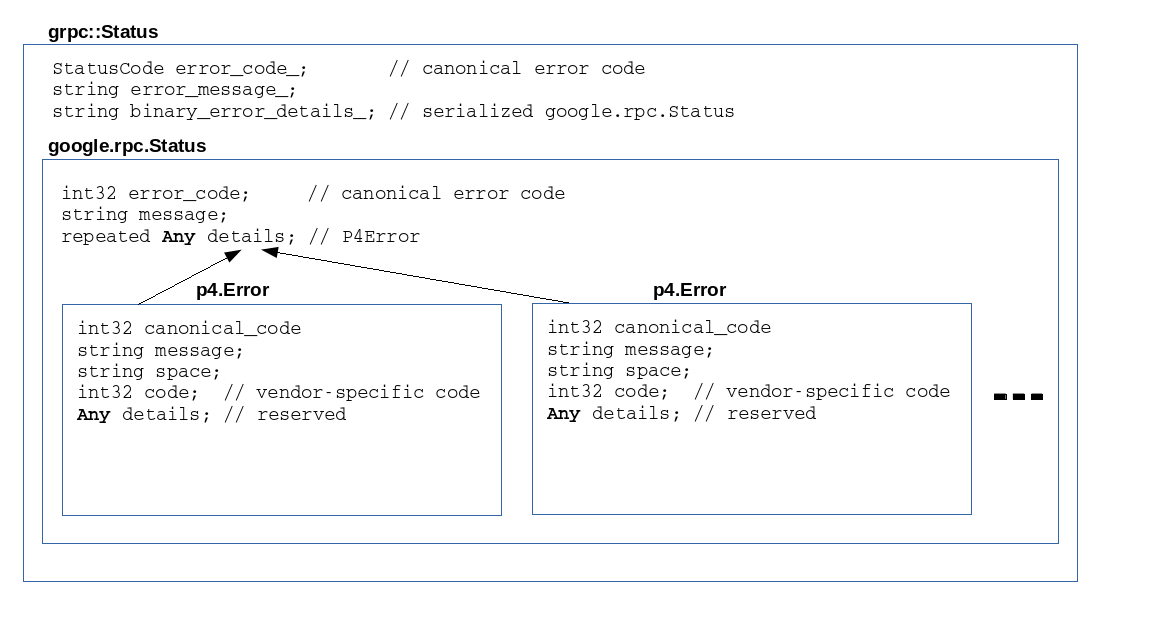
\includegraphics[keepaspectratio=true,width=\dimwidth{0.70}]{build/error-report}{}\mdline{4192}%mdk

%mdk-data-line={4193}
\mdhr{}%mdk

%mdk-data-line={4194}
\noindent\mdline{4194}\mdcaption{\textbf{Figure~\mdcaptionlabel{7}.}~\mdcaptiontext{P4Runtime Error Report Message Format}}%mdk
%mdk
\end{mdcenter}\label{fig-error-report}%mdk
%mdk
\end{figure}%mdk

%mdk-data-line={4196}
\noindent\mdline{4196}gRPC provides utility functions \mdline{4196}\mdcode{{\mdfontfamily{LuxiMono}{\mdfontsize{\dimfont{0.75}}ExtractErrorDetails()}}}\mdline{4196} and \mdline{4196}\mdcode{{\mdfontfamily{LuxiMono}{\mdfontsize{\dimfont{0.75}}SetErrorDetails()}}}\mdline{4196}
\mdline{4197}[\mdcite{grpcerrordetails}{31}]\mdline{4197} to easily convert between \mdline{4197}\mdcode{{\mdfontfamily{LuxiMono}{\mdfontsize{\dimfont{0.75}}grpc::Status}}}\mdline{4197} and
\mdline{4198}\mdcode{{\mdfontfamily{LuxiMono}{\mdfontsize{\dimfont{0.75}}google.rpc.Status}}}\mdline{4198}.%mdk

%mdk-data-line={4200}
\mdline{4200}Please see sections on individual P4Runtime RPCs for details on how
\mdline{4201}\mdcode{{\mdfontfamily{LuxiMono}{\mdfontsize{\dimfont{0.75}}grpc::Status}}}\mdline{4201} is populated for reporting errors.%mdk

%mdk-data-line={4203}
\mdline{4203}Note that P4Runtime also provides a way for the server to asynchronously report
errors which occur when processing stream messages from the client. This
error-reporting mechanism is orthogonal to the one described in this section,
which applies to unary RPCs. See the section on\mdline{4206}~\mdref{sec-stream-error-reporting}{Stream Error
Reporting}\mdline{4207} for more information.%mdk

%mdk-data-line={4209}
\section{\mdline{4209}11.\hspace*{0.5em}\mdline{4209}Atomicity of Individual \mdline{4209}\mdcode{{\mdfontfamily{LuxiMono}{\mdfontsize{\dimfont{0.75}}Write}}}\mdline{4209} and \mdline{4209}\mdcode{{\mdfontfamily{LuxiMono}{\mdfontsize{\dimfont{0.75}}Read}}}\mdline{4209} Operations}\label{sec-atomicity-of-individual-write-and-read-operations}%mdk%mdk

%mdk-data-line={4211}
\noindent\mdline{4211}Each individual entity in a batch is guaranteed to be read or written atomically
relative to packet forwarding. For example, for every table data plane \mdline{4212}\mdcode{{\mdfontfamily{LuxiMono}{\mdfontsize{\dimfont{0.75}}apply}}}\mdline{4212}
operation, and every single \mdline{4213}\mdcode{{\mdfontfamily{LuxiMono}{\mdfontsize{\dimfont{0.75}}Write}}}\mdline{4213} operation on a table that inserts, deletes,
or modifies one table entry, the \mdline{4214}\mdcode{{\mdfontfamily{LuxiMono}{\mdfontsize{\dimfont{0.75}}apply}}}\mdline{4214} operation should behave as if that
\mdline{4215}\mdcode{{\mdfontfamily{LuxiMono}{\mdfontsize{\dimfont{0.75}}Write}}}\mdline{4215} operation has not yet occurred, or as if the \mdline{4215}\mdcode{{\mdfontfamily{LuxiMono}{\mdfontsize{\dimfont{0.75}}Write}}}\mdline{4215} operation is
complete. The P4 program should never behave as if the \mdline{4216}\mdcode{{\mdfontfamily{LuxiMono}{\mdfontsize{\dimfont{0.75}}Write}}}\mdline{4216} operation is
partially complete. These guarantees also apply to extern instances: \mdline{4217}\mdcode{{\mdfontfamily{LuxiMono}{\mdfontsize{\dimfont{0.75}}Read}}}\mdline{4217} and
\mdline{4218}\mdcode{{\mdfontfamily{LuxiMono}{\mdfontsize{\dimfont{0.75}}Write}}}\mdline{4218} operations on extern entities must execute atomically relative to extern
data plane methods.%mdk

%mdk-data-line={4221}
\mdline{4221}The atomicity guarantees provided by P4Runtime for individual \mdline{4221}\mdcode{{\mdfontfamily{LuxiMono}{\mdfontsize{\dimfont{0.75}}Read}}}\mdline{4221} and \mdline{4221}\mdcode{{\mdfontfamily{LuxiMono}{\mdfontsize{\dimfont{0.75}}Write}}}\mdline{4221}
operations are the same as the guarantees required by PSA and are described in
details in the PSA specification\mdline{4223}~[\mdcite{psaatomicityofcontrolplaneops}{22}]\mdline{4223}.%mdk

%mdk-data-line={4225}
\mdline{4225}The P4\mdline{4225}\mdsub{16}\mdline{4225} language introduces an \mdline{4225}\mdcode{{\mdfontfamily{LuxiMono}{\mdfontsize{\dimfont{0.75}}@atomic}}}\mdline{4225} annotation\mdline{4225}~[\mdcite{p4concurrency}{13}]\mdline{4225}, to
guarantee atomic data plane execution of entire blocks of P4 code. P4Runtime
implementations are required to honor the \mdline{4227}\mdcode{{\mdfontfamily{LuxiMono}{\mdfontsize{\dimfont{0.75}}@atomic}}}\mdline{4227} annotation for \mdline{4227}\mdcode{{\mdfontfamily{LuxiMono}{\mdfontsize{\dimfont{0.75}}Write}}}\mdline{4227}
operations, as well as\mdline{4228}~\mdref{wildcard-reads}{non-wildcard \mdcode{{\mdfontfamily{LuxiMono}{\mdfontsize{\dimfont{0.75}}Read}}} operations}\mdline{4228},
relative to data plane execution. Consider the following P4 example written for
PSA:%mdk

%mdk-data-line={4232}
\begin{mdbmargintb}{6pt}{6pt}%mdk
\begin{mdblock}{padding=6pt,border-width=0.5pt,border-style=solid,background-color=\#FFFFDD,breakable=true}%mdk
%mdk-data-line={4233}
\begin{mdpre}%mdk
\noindent{\mdfontfamily{LuxiMono}{\mdfontsize{\dimfont{0.75}}{\bfseries{\mdcolor{navy}control}}~C{\mdcolor{purple}1}~\{\\
~~{\bfseries{\mdcolor{navy}typedef}}~{\bfseries{\mdcolor{navy}bit}}\textless{}{\mdcolor{purple}10}\textgreater{}~Index\_t;\\
~~{\bfseries{\mdcolor{navy}typedef}}~{\bfseries{\mdcolor{navy}bit}}\textless{}{\mdcolor{purple}32}\textgreater{}~Value\_t;\\
~~Register\textless{}Value\_t,~Index\_t\textgreater{}({\mdcolor{purple}32}w1024)~r1;\\
\\
~~{\bfseries{\mdcolor{navy}apply}}~\{\\
~~~~{\mdcolor{darkgreen}//~...}\\
{\mdcolor{navy}~~~~@}{\mdcolor{navy}atomic}{\mdcolor{maroon}~\{}\\
~~~~~~~~Value\_t~v~=~r1.read((Index\_t){\mdcolor{purple}1});\\
~~~~~~~~v~=~v~+~{\mdcolor{purple}1};\\
~~~~~~~~r1.write((Index\_t){\mdcolor{purple}1},~v);\\
~~~~\}\\
~~\}\\
\}}}%mdk
\end{mdpre}%mdk%mdk
\end{mdblock}%mdk
\end{mdbmargintb}%mdk

%mdk-data-line={4249}
\noindent\mdline{4249}If a P4Runtime server is processing messages which write to Register \mdline{4249}\mdcode{{\mdfontfamily{LuxiMono}{\mdfontsize{\dimfont{0.75}}r1}}}\mdline{4249} at
index \mdline{4250}\mdcode{{\mdfontfamily{LuxiMono}{\mdfontsize{\dimfont{0.75}}1}}}\mdline{4250}, these writes must not happen between the data plane \mdline{4250}\mdcode{{\mdfontfamily{LuxiMono}{\mdfontsize{\dimfont{0.75}}read}}}\mdline{4250} and
\mdline{4251}\mdcode{{\mdfontfamily{LuxiMono}{\mdfontsize{\dimfont{0.75}}write}}}\mdline{4251}.%mdk

%mdk-data-line={4253}
\mdline{4253}Now let\mdline{4253}'\mdline{4253}s consider the following example:%mdk

%mdk-data-line={4255}
\begin{mdbmargintb}{6pt}{6pt}%mdk
\begin{mdblock}{padding=6pt,border-width=0.5pt,border-style=solid,background-color=\#FFFFDD,breakable=true}%mdk
%mdk-data-line={4256}
\begin{mdpre}%mdk
\noindent{\mdfontfamily{LuxiMono}{\mdfontsize{\dimfont{0.75}}{\bfseries{\mdcolor{navy}control}}~C{\mdcolor{purple}1}~\{\\
~~{\bfseries{\mdcolor{navy}typedef}}~{\bfseries{\mdcolor{navy}bit}}\textless{}{\mdcolor{purple}10}\textgreater{}~Index\_t;\\
~~{\bfseries{\mdcolor{navy}typedef}}~{\bfseries{\mdcolor{navy}bit}}\textless{}{\mdcolor{purple}32}\textgreater{}~Value\_t;\\
~~Register\textless{}Value\_t,~Index\_t\textgreater{}({\mdcolor{purple}32}w1024,~(Value\_t){\mdcolor{purple}0}~{\mdcolor{darkgreen}/*}{\mdcolor{darkgreen}~initial~value~}{\mdcolor{darkgreen}*/})~r1;\\
\\
~~{\bfseries{\mdcolor{navy}apply}}~\{\\
{\mdcolor{navy}~~~~@}{\mdcolor{navy}atomic}{\mdcolor{maroon}~\{}\\
~~~~~~~~r1.write((Index\_t){\mdcolor{purple}1},~(Value\_t){\mdcolor{purple}100});\\
~~~~~~~~r1.write((Index\_t){\mdcolor{purple}2},~(Value\_t){\mdcolor{purple}100});\\
~~~~\}\\
{\mdcolor{navy}~~~~@}{\mdcolor{navy}atomic}{\mdcolor{maroon}~\{}\\
~~~~~~~~r1.write((Index\_t){\mdcolor{purple}1},~(Value\_t){\mdcolor{purple}200});\\
~~~~~~~~r1.write((Index\_t){\mdcolor{purple}2},~(Value\_t){\mdcolor{purple}200});\\
~~~~\}\\
~~\}\\
\}}}%mdk
\end{mdpre}%mdk%mdk
\end{mdblock}%mdk
\end{mdbmargintb}%mdk

%mdk-data-line={4274}
\noindent\mdline{4274}If a P4Runtime client issues a \mdline{4274}\emph{wildcard}\mdline{4274} \mdline{4274}\mdcode{{\mdfontfamily{LuxiMono}{\mdfontsize{\dimfont{0.75}}Read}}}\mdline{4274} on Register \mdline{4274}\mdcode{{\mdfontfamily{LuxiMono}{\mdfontsize{\dimfont{0.75}}r1}}}\mdline{4274}, there is no
guarantee that \mdline{4275}\mdcode{{\mdfontfamily{LuxiMono}{\mdfontsize{\dimfont{0.75}}r1{}[1]~==~r1{}[2]}}}\mdline{4275} in the response, as the read for \mdline{4275}\mdcode{{\mdfontfamily{LuxiMono}{\mdfontsize{\dimfont{0.75}}r1{}[1]}}}\mdline{4275} may
occur after the data plane executes the first atomic block, but before the
second atomic block, and the read for \mdline{4277}\mdcode{{\mdfontfamily{LuxiMono}{\mdfontsize{\dimfont{0.75}}r1{}[2]}}}\mdline{4277} may occur after the data plane
executes the second atomic block. In other words, the server is explicitly
allowed to read \mdline{4279}\mdcode{{\mdfontfamily{LuxiMono}{\mdfontsize{\dimfont{0.75}}r1{}[1]}}}\mdline{4279} and \mdline{4279}\mdcode{{\mdfontfamily{LuxiMono}{\mdfontsize{\dimfont{0.75}}r1{}[2]}}}\mdline{4279} separately, while allowing the data plane to
perform operations on the register between those two reads. The atomicity
guarantees for a wildcard read are the same as for the equivalent batch (as one
\mdline{4282}\mdcode{{\mdfontfamily{LuxiMono}{\mdfontsize{\dimfont{0.75}}ReadRequest}}}\mdline{4282} message) of individual read requests. Similar to a batch
\mdline{4283}\mdcode{{\mdfontfamily{LuxiMono}{\mdfontsize{\dimfont{0.75}}ReadRequest}}}\mdline{4283}, a wildcard read of a register can execute the reads of the
register array elements (\mdline{4284}\mdcode{{\mdfontfamily{LuxiMono}{\mdfontsize{\dimfont{0.75}}r1{}[1]}}}\mdline{4284}, \mdline{4284}\mdcode{{\mdfontfamily{LuxiMono}{\mdfontsize{\dimfont{0.75}}r1{}[2]}}}\mdline{4284}, \mdline{4284}\dots{}\mdline{4284}) in an arbitrary order relative
to each other.%mdk

%mdk-data-line={4287}
\mdline{4287}If the \mdline{4287}\mdcode{{\mdfontfamily{LuxiMono}{\mdfontsize{\dimfont{0.75}}@atomic}}}\mdline{4287} annotation cannot be honored with the above guarantees by the
P4Runtime implementation for a P4-programmable target, we expect the P4 compiler
to reject the program.%mdk

%mdk-data-line={4291}
\section{\mdline{4291}12.\hspace*{0.5em}\mdline{4291}\mdcode{{\mdfontfamily{LuxiMono}{\mdfontsize{\dimfont{0.75}}Write}}}\mdline{4291} RPC}\label{sec-write-rpc}%mdk%mdk

%mdk-data-line={4293}
\noindent\mdline{4293}The \mdline{4293}\mdcode{{\mdfontfamily{LuxiMono}{\mdfontsize{\dimfont{0.75}}Write}}}\mdline{4293} RPC updates one or more P4 entities on the target. The request is
defined as follows:%mdk

%mdk-data-line={4296}
\begin{mdbmargintb}{6pt}{6pt}%mdk
\begin{mdblock}{padding=6pt,border-width=0.5pt,border-style=solid,background-color=\#E6FFFF,breakable=true}%mdk
%mdk-data-line={4297}
\begin{mdpre}%mdk
\noindent{\mdfontfamily{LuxiMono}{\mdfontsize{\dimfont{0.75}}{\bfseries{\mdcolor{navy}message}}~WriteRequest~\{\\
~~{\bfseries{\mdcolor{navy}uint64}}~device\_id~{\bfseries{\mdcolor{navy}=}}~{\mdcolor{purple}1};\\
~~{\bfseries{\mdcolor{navy}uint64}}~role\_id~{\bfseries{\mdcolor{navy}=}}~{\mdcolor{purple}2};\\
~~Uint128~election\_id~{\bfseries{\mdcolor{navy}=}}~{\mdcolor{purple}3};\\
~~{\bfseries{\mdcolor{navy}repeated}}~Update~updates~{\bfseries{\mdcolor{navy}=}}~{\mdcolor{purple}4};\\
~~{\bfseries{\mdcolor{navy}enum}}~Atomicity~\{\\
~~~~CONTINUE\_ON\_ERROR~{\bfseries{\mdcolor{navy}=}}~{\mdcolor{purple}0};\\
~~~~ROLLBACK\_ON\_ERROR~{\bfseries{\mdcolor{navy}=}}~{\mdcolor{purple}1};\\
~~~~DATAPLANE\_ATOMIC~{\bfseries{\mdcolor{navy}=}}~{\mdcolor{purple}2};\\
~~\}\\
~~Atomicity~atomicity~{\bfseries{\mdcolor{navy}=}}~{\mdcolor{purple}5};\\
\}}}%mdk
\end{mdpre}%mdk%mdk
\end{mdblock}%mdk
\end{mdbmargintb}%mdk

%mdk-data-line={4311}
\noindent\mdline{4311}The \mdline{4311}\mdcode{{\mdfontfamily{LuxiMono}{\mdfontsize{\dimfont{0.75}}device\_id}}}\mdline{4311} uniquely identifies the target P4 device. The \mdline{4311}\mdcode{{\mdfontfamily{LuxiMono}{\mdfontsize{\dimfont{0.75}}role\_id}}}\mdline{4311} and
\mdline{4312}\mdcode{{\mdfontfamily{LuxiMono}{\mdfontsize{\dimfont{0.75}}election\_id}}}\mdline{4312} define the client role and election-id as described in the
\mdline{4313}\mdref{sec-master-slave-arbitration-and-controller-replication}{Master-Slave Arbitration and Controller
Replication}\mdline{4314}
section. The server is expected to perform the following checks (in this order)
before processing the \mdline{4316}\mdcode{{\mdfontfamily{LuxiMono}{\mdfontsize{\dimfont{0.75}}updates}}}\mdline{4316} list:%mdk

%mdk-data-line={4318}
\begin{enumerate}%mdk

%mdk-data-line={4318}
\item{}
%mdk-data-line={4318}
\mdline{4318}If \mdline{4318}\mdcode{{\mdfontfamily{LuxiMono}{\mdfontsize{\dimfont{0.75}}device\_id}}}\mdline{4318} does not match any of the devices known to the P4Runtime
server or if \mdline{4319}\mdcode{{\mdfontfamily{LuxiMono}{\mdfontsize{\dimfont{0.75}}role\_id}}}\mdline{4319} does not match any of the roles for the device, the
server must return a \mdline{4320}\mdcode{{\mdfontfamily{LuxiMono}{\mdfontsize{\dimfont{0.75}}NOT\_FOUND}}}\mdline{4320} error.%mdk%mdk

%mdk-data-line={4322}
\item{}
%mdk-data-line={4322}
\mdline{4322}If the client is not the master for (\mdline{4322}\mdcode{{\mdfontfamily{LuxiMono}{\mdfontsize{\dimfont{0.75}}device\_id}}}\mdline{4322}, \mdline{4322}\mdcode{{\mdfontfamily{LuxiMono}{\mdfontsize{\dimfont{0.75}}role\_id}}}\mdline{4322}) according to the
\mdline{4323}\mdcode{{\mdfontfamily{LuxiMono}{\mdfontsize{\dimfont{0.75}}election\_id}}}\mdline{4323} value, the server must return a \mdline{4323}\mdcode{{\mdfontfamily{LuxiMono}{\mdfontsize{\dimfont{0.75}}PERMISSION\_DENIED}}}\mdline{4323} error.%mdk%mdk

%mdk-data-line={4325}
\item{}
%mdk-data-line={4325}
\mdline{4325}If the \mdline{4325}\mdcode{{\mdfontfamily{LuxiMono}{\mdfontsize{\dimfont{0.75}}Write}}}\mdline{4325} is attempted before a \mdline{4325}\mdcode{{\mdfontfamily{LuxiMono}{\mdfontsize{\dimfont{0.75}}ForwardingPipelineConfig}}}\mdline{4325} has been set,
the server must return a \mdline{4326}\mdcode{{\mdfontfamily{LuxiMono}{\mdfontsize{\dimfont{0.75}}FAILED\_PRECONDITION}}}\mdline{4326} error.%mdk%mdk
%mdk
\end{enumerate}%mdk

%mdk-data-line={4328}
\noindent\mdline{4328}The updates field is a list of P4 entity updates to be applied. Each update is
defined as:%mdk

%mdk-data-line={4331}
\begin{mdbmargintb}{6pt}{6pt}%mdk
\begin{mdblock}{padding=6pt,border-width=0.5pt,border-style=solid,background-color=\#E6FFFF,breakable=true}%mdk
%mdk-data-line={4332}
\begin{mdpre}%mdk
\noindent{\mdfontfamily{LuxiMono}{\mdfontsize{\dimfont{0.75}}{\bfseries{\mdcolor{navy}message}}~Update~\{\\
~~{\bfseries{\mdcolor{navy}enum}}~Type~\{\\
~~~~UNSPECIFIED~{\bfseries{\mdcolor{navy}=}}~{\mdcolor{purple}0};\\
~~~~INSERT~{\bfseries{\mdcolor{navy}=}}~{\mdcolor{purple}1};\\
~~~~MODIFY~{\bfseries{\mdcolor{navy}=}}~{\mdcolor{purple}2};\\
~~~~DELETE~{\bfseries{\mdcolor{navy}=}}~{\mdcolor{purple}3};\\
~~\}\\
~~Type~type~{\bfseries{\mdcolor{navy}=}}~{\mdcolor{purple}1};\\
~~Entity~entity~{\bfseries{\mdcolor{navy}=}}~{\mdcolor{purple}2};\\
\}}}%mdk
\end{mdpre}%mdk%mdk
\end{mdblock}%mdk
\end{mdbmargintb}%mdk

%mdk-data-line={4344}
\noindent\mdline{4344}This is modeled as performing an update operation on the given entity against
its entity container. The entity container is either a \mdline{4345}\emph{logical}\mdline{4345} table (\mdline{4345}e.g.\mdline{4345}
\mdline{4346}\mdcode{{\mdfontfamily{LuxiMono}{\mdfontsize{\dimfont{0.75}}CounterEntry}}}\mdline{4346}) or an actual table (\mdline{4346}e.g.\mdline{4346} \mdline{4346}\mdcode{{\mdfontfamily{LuxiMono}{\mdfontsize{\dimfont{0.75}}TableEntry}}}\mdline{4346}) in the P4 data
plane. Each entity in the container is uniquely identified by its \mdline{4347}\emph{key}\mdline{4347}. Please
refer to the\mdline{4348}~\mdref{sec-p4-entity-msgs}{P4 Entity Messages}\mdline{4348} section for details on
what parts of the entity specification make up the \mdline{4349}\emph{key}\mdline{4349} for each P4 entity.%mdk

%mdk-data-line={4351}
\mdline{4351}An update can be one of the following types:%mdk

%mdk-data-line={4353}
\begin{itemize}%mdk

%mdk-data-line={4353}
\item{}
%mdk-data-line={4353}
\mdline{4353}\mdcode{{\mdfontfamily{LuxiMono}{\mdfontsize{\dimfont{0.75}}INSERT}}}\mdline{4353}: Inserts the given P4 entity in the entity container.
The \mdline{4354}\mdcode{{\mdfontfamily{LuxiMono}{\mdfontsize{\dimfont{0.75}}entity}}}\mdline{4354} field always specifies the full state of the P4 entity.
If the entity already exists, an \mdline{4355}\mdcode{{\mdfontfamily{LuxiMono}{\mdfontsize{\dimfont{0.75}}ALREADY\_EXISTS}}}\mdline{4355} error is returned, and
the existing entity remains unchanged.
If the entity is malformed, an \mdline{4357}\mdcode{{\mdfontfamily{LuxiMono}{\mdfontsize{\dimfont{0.75}}INVALID\_ARGUMENT}}}\mdline{4357} error is returned.
If the entity cannot be inserted because the container is already full,
a \mdline{4359}\mdcode{{\mdfontfamily{LuxiMono}{\mdfontsize{\dimfont{0.75}}RESOURCE\_EXHAUSTED}}}\mdline{4359} error is returned.%mdk%mdk

%mdk-data-line={4361}
\item{}
%mdk-data-line={4361}
\mdline{4361}\mdcode{{\mdfontfamily{LuxiMono}{\mdfontsize{\dimfont{0.75}}MODIFY}}}\mdline{4361}: Modifies the P4 entity to its new specified state. This uses
\mdline{4362}\emph{assign}\mdline{4362} or \mdline{4362}\emph{full-snapshot}\mdline{4362} semantics, \mdline{4362}i.e.\mdline{4362} the entity field contains the
complete new state of the entity, not a diff from its previous state. If the
entity is malformed, an \mdline{4364}\mdcode{{\mdfontfamily{LuxiMono}{\mdfontsize{\dimfont{0.75}}INVALID\_ARGUMENT}}}\mdline{4364} error is usually returned (unless a
more specific error code applies\mdline{4365}~[\mdcite{grpcstatuscodes}{32}]\mdline{4365}). If the entity does not
exist, a \mdline{4366}\mdcode{{\mdfontfamily{LuxiMono}{\mdfontsize{\dimfont{0.75}}NOT\_FOUND}}}\mdline{4366} error is returned.%mdk%mdk

%mdk-data-line={4368}
\item{}
%mdk-data-line={4368}
\mdline{4368}\mdcode{{\mdfontfamily{LuxiMono}{\mdfontsize{\dimfont{0.75}}DELETE}}}\mdline{4368}: Deletes the specified P4 entity. If the entity does not exist, a
\mdline{4369}\mdcode{{\mdfontfamily{LuxiMono}{\mdfontsize{\dimfont{0.75}}NOT\_FOUND}}}\mdline{4369} error is returned. In order to delete, the entity specification
only needs to include the key. Any non-key parts of entity are ignored.%mdk%mdk
%mdk
\end{itemize}%mdk

%mdk-data-line={4372}
\noindent\mdline{4372}If an update is not allowed under the given controller role, the server must
return a \mdline{4373}\mdcode{{\mdfontfamily{LuxiMono}{\mdfontsize{\dimfont{0.75}}PERMISSION\_DENIED}}}\mdline{4373} error for this update.%mdk

%mdk-data-line={4375}
\subsection{\mdline{4375}12.1.\hspace*{0.5em}\mdline{4375}Batching and Ordering of Updates}\label{sec-batching-and-ordering-of-updates}%mdk%mdk

%mdk-data-line={4377}
\noindent\mdline{4377}P4Runtime supports batching of \mdline{4377}\mdcode{{\mdfontfamily{LuxiMono}{\mdfontsize{\dimfont{0.75}}Write}}}\mdline{4377} operations. The list of updates in a
\mdline{4378}\mdcode{{\mdfontfamily{LuxiMono}{\mdfontsize{\dimfont{0.75}}WriteRequest}}}\mdline{4378} is referred to as a \mdline{4378}\emph{batch}\mdline{4378}. A batch can consist of arbitrary
updates on an arbitrary set of P4 entities. It is not restricted to a particular
entity or table (in the case of \mdline{4380}\mdcode{{\mdfontfamily{LuxiMono}{\mdfontsize{\dimfont{0.75}}TableEntry}}}\mdline{4380} entities).%mdk

%mdk-data-line={4382}
\mdline{4382}The P4Runtime server may choose to reorder updates in a batch when processing
them, and/or process updates in parallel.  Updates across multiple concurrent
\mdline{4384}\mdcode{{\mdfontfamily{LuxiMono}{\mdfontsize{\dimfont{0.75}}WriteRequest}}}\mdline{4384}s can also be processed interleaved and/or in parallel.
However, \mdline{4385}\textbf{the processing of updates must be strictly serializable}\mdline{4385}.  That
is, given a history \mdline{4386}$S$\mdline{4386} of \mdline{4386}\mdcode{{\mdfontfamily{LuxiMono}{\mdfontsize{\dimfont{0.75}}WriteRequest}}}\mdline{4386}s including the responses to those
requests, there must exist an order \mdline{4387}$L$\mdline{4387} for all updates in \mdline{4387}$S$\mdline{4387}, such that:%mdk

%mdk-data-line={4389}
\begin{enumerate}[noitemsep,topsep=\mdcompacttopsep]%mdk

%mdk-data-line={4389}
\item\mdline{4389}For two updates \mdline{4389}$u_1$\mdline{4389} and \mdline{4389}$u_2$\mdline{4389}, if the write request containing \mdline{4389}$u_1$\mdline{4389}
completed before the write request of \mdline{4390}$u_2$\mdline{4390} was sent, then \mdline{4390}$u_1$\mdline{4390} must appear
before \mdline{4391}$u_2$\mdline{4391} in \mdline{4391}$L$\mdline{4391}.%mdk

%mdk-data-line={4392}
\item\mdline{4392}Executing all updates in \mdline{4392}$L$\mdline{4392} sequentially must yield the same response for
every update as in \mdline{4393}$S$\mdline{4393}.%mdk

%mdk-data-line={4394}
\item\mdline{4394}The observable state of the switch after \mdline{4394}$S$\mdline{4394} (\mdline{4394}e.g.\mdline{4394}, through the \mdline{4394}\mdcode{{\mdfontfamily{LuxiMono}{\mdfontsize{\dimfont{0.75}}Read}}}\mdline{4394} RPC)
is identical to the one obtained by sequentially executing \mdline{4395}$L$\mdline{4395}.%mdk
%mdk
\end{enumerate}%mdk

%mdk-data-line={4397}
\noindent\mdline{4397}The \mdline{4397}\mdcode{{\mdfontfamily{LuxiMono}{\mdfontsize{\dimfont{0.75}}Write}}}\mdline{4397} RPC demarcates the batch boundary, and can be used to ensure
ordering between dependent updates. When the \mdline{4398}\mdcode{{\mdfontfamily{LuxiMono}{\mdfontsize{\dimfont{0.75}}Write}}}\mdline{4398} RPC returns, it is required
that all operations in the batch have been committed to the P4 data plane,
with the exception of any operations that return an error status.
If two updates from the client depend on each other (\mdline{4401}e.g.\mdline{4401} inserting an
\mdline{4402}\mdcode{{\mdfontfamily{LuxiMono}{\mdfontsize{\dimfont{0.75}}ActionProfileMember}}}\mdline{4402} followed by pointing a \mdline{4402}\mdcode{{\mdfontfamily{LuxiMono}{\mdfontsize{\dimfont{0.75}}TableEntry}}}\mdline{4402} to it) and the updates
are not split into separate batches, then the behavior may be non-deterministic.
Similarly, clients can invoke multiple outstanding \mdline{4404}\mdcode{{\mdfontfamily{LuxiMono}{\mdfontsize{\dimfont{0.75}}Write}}}\mdline{4404} RPCs. If the updates
across these RPCs have dependencies, the observed behavior may be
non-deterministic. For this reason, most clients are advised to split dependent
updates across separate Write calls. Additionally, each Write call has to be
sent sequentially, waiting for the previous call to be acknowledged before
sending the next one.%mdk

%mdk-data-line={4412}
\subsection{\mdline{4412}12.2.\hspace*{0.5em}\mdline{4412}Batch Atomicity}\label{sec-batch-atomicity}%mdk%mdk

%mdk-data-line={4414}
\noindent\mdline{4414}A P4Runtime server may arbitrarily reorder messages within a batch. The
atomicity semantics of the batch operations are defined by the \mdline{4415}\mdcode{{\mdfontfamily{LuxiMono}{\mdfontsize{\dimfont{0.75}}Atomicity}}}\mdline{4415}
enum. A P4Runtime server is required to support only the modes marked as
\mdline{4417}\emph{Required}\mdline{4417} below:%mdk

%mdk-data-line={4419}
\begin{itemize}%mdk

%mdk-data-line={4419}
\item{}
%mdk-data-line={4419}
\mdline{4419}\emph{Required}\mdline{4419}: \mdline{4419}\mdcode{{\mdfontfamily{LuxiMono}{\mdfontsize{\dimfont{0.75}}CONTINUE\_ON\_ERROR}}}\mdline{4419}: This is the default behavior and the default
enum value. Each operation within the batch must be attempted even if one or
more encounter errors. Every data plane packet is guaranteed to be processed
according to table contents as they are between two individual operations of
the batch, but there could be several packets processed that \mdline{4423}\emph{see}\mdline{4423} each of
these intermediate stages.%mdk%mdk

%mdk-data-line={4426}
\item{}
%mdk-data-line={4426}
\mdline{4426}\emph{Optional}\mdline{4426}: \mdline{4426}\mdcode{{\mdfontfamily{LuxiMono}{\mdfontsize{\dimfont{0.75}}ROLLBACK\_ON\_ERROR}}}\mdline{4426}: Operations within the batch are attempted in
an arbitrary order (each committed to data plane) until the target detects an
error. At this point, the target must roll back the operations such that both
software and data plane state is consistent with the state before the batch
was attempted. The resulting behavior is \mdline{4430}\emph{all-or-none}\mdline{4430}, except the batch is
not atomic from a data plane point of view. Every data plane packet is
guaranteed to be processed according to table contents as they are between two
individual operations of the batch, but there could be several packets
processed that \mdline{4434}\emph{see}\mdline{4434} each of these intermediate stages. The details and design
of the rollback mechanism are outside the scope of this specification. One
possibility is to create a shadow copy of both the software and hardware state
at the start, and restore it upon failure.%mdk

%mdk-data-line={4439}
\mdline{4439}If a P4Runtime server does not support this option at all, an
\mdline{4440}\mdcode{{\mdfontfamily{LuxiMono}{\mdfontsize{\dimfont{0.75}}UNIMPLEMENTED}}}\mdline{4440} error is returned at all times. If a P4Runtime
supports some batches in an rollback way but not others (\mdline{4441}e.g.\mdline{4441} it is
more straightforward to implement batches that contain only \mdline{4442}\mdcode{{\mdfontfamily{LuxiMono}{\mdfontsize{\dimfont{0.75}}INSERT}}}\mdline{4442}
operations, vs. those that contain \mdline{4443}\mdcode{{\mdfontfamily{LuxiMono}{\mdfontsize{\dimfont{0.75}}DELETE}}}\mdline{4443} operations), an
\mdline{4444}\mdcode{{\mdfontfamily{LuxiMono}{\mdfontsize{\dimfont{0.75}}UNIMPLEMENTED}}}\mdline{4444} error is returned when the batch cannot be executed
in a data plane-atomic way.%mdk%mdk

%mdk-data-line={4447}
\item{}
%mdk-data-line={4447}
\mdline{4447}\emph{Optional}\mdline{4447}: \mdline{4447}\mdcode{{\mdfontfamily{LuxiMono}{\mdfontsize{\dimfont{0.75}}DATAPLANE\_ATOMIC}}}\mdline{4447}: This is the strictest requirement where the
entire batch must be atomic from a data plane point of view. Every data plane
packet is guaranteed to be processed according to table contents before the
batch began, or after the batch completes. The batch is therefore treated as a
\mdline{4451}\emph{transaction}\mdline{4451}. The details and design of how to achieve data plane-atomicity
is outside the scope of this specification. One possibility is to limit the
target to half of the data plane\mdline{4453}'\mdline{4453}s table capacity at all times. At the start
of the batch processing, the remaining half of the table capacity can be
initialized with the current table state and used as a working area to commit
all operations within the batch. At the end (if there were no errors), a
simple pointer-swap like approach can be used to switch to this half of the
table.%mdk

%mdk-data-line={4460}
\mdline{4460}If a P4Runtime server does not support this option at all, an \mdline{4460}\mdcode{{\mdfontfamily{LuxiMono}{\mdfontsize{\dimfont{0.75}}UNIMPLEMENTED}}}\mdline{4460}
error is returned at all times. If a P4Runtime supports some batches in an
atomic way but not others, an \mdline{4462}\mdcode{{\mdfontfamily{LuxiMono}{\mdfontsize{\dimfont{0.75}}UNIMPLEMENTED}}}\mdline{4462} error is returned when the batch
cannot be executed in a data plane-atomic way.%mdk%mdk
%mdk
\end{itemize}%mdk

%mdk-data-line={4465}
\noindent\mdline{4465}There is no expectation that a given client must always use the same \mdline{4465}\mdcode{{\mdfontfamily{LuxiMono}{\mdfontsize{\dimfont{0.75}}Atomicity}}}\mdline{4465}
enum value. At any given time, the client is free to compose batches and assign
atomicity mode as it sees fit. For example, for a set of entities, a client may
decide to use \mdline{4468}\mdcode{{\mdfontfamily{LuxiMono}{\mdfontsize{\dimfont{0.75}}DATAPLANE\_ATOMIC}}}\mdline{4468} at one time and default behavior
(\mdline{4469}\mdcode{{\mdfontfamily{LuxiMono}{\mdfontsize{\dimfont{0.75}}CONTINUE\_ON\_ERROR}}}\mdline{4469}) at other times.%mdk

%mdk-data-line={4471}
\subsection{\mdline{4471}12.3.\hspace*{0.5em}\mdline{4471}Error Reporting}\label{sec-error-reporting}%mdk%mdk

%mdk-data-line={4473}
\noindent\mdline{4473}Please see section\mdline{4473}~\mdref{sec-error-reporting-messages}{Error Reporting Messages}\mdline{4473} for
information on error reporting messages and guidelines. P4Runtime server will
populate \mdline{4475}\mdcode{{\mdfontfamily{LuxiMono}{\mdfontsize{\dimfont{0.75}}grpc::Status}}}\mdline{4475} as follows:%mdk

%mdk-data-line={4477}
\begin{enumerate}%mdk

%mdk-data-line={4477}
\item{}
%mdk-data-line={4477}
\mdline{4477}If all batch updates succeeded, set \mdline{4477}\mdcode{{\mdfontfamily{LuxiMono}{\mdfontsize{\dimfont{0.75}}grpc::Status::code\_}}}\mdline{4477} to \mdline{4477}\mdcode{{\mdfontfamily{LuxiMono}{\mdfontsize{\dimfont{0.75}}OK}}}\mdline{4477} and do not
populate any other field.%mdk%mdk

%mdk-data-line={4480}
\item{}
%mdk-data-line={4480}
\mdline{4480}If an error is encountered before even trying to attempt individual batch
updates, set \mdline{4481}\mdcode{{\mdfontfamily{LuxiMono}{\mdfontsize{\dimfont{0.75}}grpc::Status::code\_}}}\mdline{4481} that best describes that RPC-wide
error. For example, use \mdline{4482}\mdcode{{\mdfontfamily{LuxiMono}{\mdfontsize{\dimfont{0.75}}UNAVAILABLE}}}\mdline{4482} if the P4Runtime service is not yet
ready to handle requests. Set \mdline{4483}\mdcode{{\mdfontfamily{LuxiMono}{\mdfontsize{\dimfont{0.75}}error\_message\_}}}\mdline{4483} to describe the issue. Do not
set \mdline{4484}\mdcode{{\mdfontfamily{LuxiMono}{\mdfontsize{\dimfont{0.75}}error\_details}}}\mdline{4484} in this case.%mdk%mdk

%mdk-data-line={4486}
\item{}
%mdk-data-line={4486}
\mdline{4486}Otherwise, if one or more updates in the batch (\mdline{4486}\mdcode{{\mdfontfamily{LuxiMono}{\mdfontsize{\dimfont{0.75}}WriteRequest.updates}}}\mdline{4486})
failed, set \mdline{4487}\mdcode{{\mdfontfamily{LuxiMono}{\mdfontsize{\dimfont{0.75}}grpc::Status::code\_}}}\mdline{4487} to \mdline{4487}\mdcode{{\mdfontfamily{LuxiMono}{\mdfontsize{\dimfont{0.75}}UNKNOWN}}}\mdline{4487}. For example, one update in
the batch may fail with \mdline{4488}\mdcode{{\mdfontfamily{LuxiMono}{\mdfontsize{\dimfont{0.75}}RESOURCE\_EXHAUSTED}}}\mdline{4488} and another with
\mdline{4489}\mdcode{{\mdfontfamily{LuxiMono}{\mdfontsize{\dimfont{0.75}}INVALID\_ARGUMENT}}}\mdline{4489}. A \mdline{4489}\mdcode{{\mdfontfamily{LuxiMono}{\mdfontsize{\dimfont{0.75}}p4.Error}}}\mdline{4489} message is used to capture the status of
each and every update in the batch. The number of \mdline{4490}\mdcode{{\mdfontfamily{LuxiMono}{\mdfontsize{\dimfont{0.75}}p4.Error}}}\mdline{4490} messages packed
into \mdline{4491}\mdcode{{\mdfontfamily{LuxiMono}{\mdfontsize{\dimfont{0.75}}google.rpc.Status.details}}}\mdline{4491} field should therefore always match the
number of updates in the \mdline{4492}\mdcode{{\mdfontfamily{LuxiMono}{\mdfontsize{\dimfont{0.75}}WriteRequest}}}\mdline{4492}, and the order of
\mdline{4493}\mdcode{{\mdfontfamily{LuxiMono}{\mdfontsize{\dimfont{0.75}}p4.Error}}}\mdline{4493} messages must be in the same order as the corresponding
updates. If some of the updates were successful, the corresponding
\mdline{4495}\mdcode{{\mdfontfamily{LuxiMono}{\mdfontsize{\dimfont{0.75}}p4.Error}}}\mdline{4495} should set the code to \mdline{4495}\mdcode{{\mdfontfamily{LuxiMono}{\mdfontsize{\dimfont{0.75}}OK}}}\mdline{4495} and omit other fields.%mdk%mdk
%mdk
\end{enumerate}%mdk

%mdk-data-line={4497}
\begin{mdbmargintb}{6pt}{6pt}%mdk
\begin{mdblock}{padding=6pt,border-width=0.5pt,border-style=solid,background-color=\#E6FFFF,breakable=true}%mdk
%mdk-data-line={4498}
\begin{mdpre}%mdk
\noindent{\mdfontfamily{LuxiMono}{\mdfontsize{\dimfont{0.75}}{\mdcolor{darkgreen}\#~Example~of~a~grpc::Status~returned~for~a~Write~RPC~with~a~batch~of~3~updates.}\\
{\mdcolor{darkgreen}\#~The~first~and~third~updates~encountered~an~error,~while~the~second~update}\\
{\mdcolor{darkgreen}\#~succeeded.}\\
code\_~=~{\mdcolor{purple}2}~~{\mdcolor{darkgreen}\#~UNKNOWN}\\
error\_message\_~=~{\mdcolor{maroon}"}{\mdcolor{maroon}Write~failure.}{\mdcolor{maroon}"}\\
binary\_error\_details~\{\\
~~code:~{\mdcolor{purple}2}~~{\mdcolor{darkgreen}\#~UNKNOWN}\\
~~message:~{\mdcolor{maroon}"}{\mdcolor{maroon}Write~failure.}{\mdcolor{maroon}"}\\
~~details~\{\\
~~~~canonical\_code:~{\mdcolor{purple}8}~~{\mdcolor{darkgreen}\#~RESOURCE\_EXHAUSTED}\\
~~~~message:~{\mdcolor{maroon}"}{\mdcolor{maroon}Table~is~full.}{\mdcolor{maroon}"}\\
~~~~space:~{\mdcolor{maroon}"}{\mdcolor{maroon}targetX-psa-vendorY}{\mdcolor{maroon}"}\\
~~~~code:~{\mdcolor{purple}500}~~{\mdcolor{darkgreen}\#~ERR\_TABLE\_FULL}\\
~~\}\\
~~details~\{\\
~~~~canonical\_code:~{\mdcolor{purple}0}~~{\mdcolor{darkgreen}\#~OK}\\
~~\}\\
~~details~\{\\
~~~~canonical\_code:~{\mdcolor{purple}6}~~{\mdcolor{darkgreen}\#~ALREADY\_EXISTS}\\
~~~~message:~{\mdcolor{maroon}"}{\mdcolor{maroon}Entity~already~exists.}{\mdcolor{maroon}"}\\
~~~~space:~{\mdcolor{maroon}"}{\mdcolor{maroon}targetX-psa-vendorY}{\mdcolor{maroon}"}\\
~~~~code:~{\mdcolor{purple}600}~~{\mdcolor{darkgreen}\#~ERR\_ENTITY\_ALREADY\_EXISTS}\\
~~\}\\
\}}}%mdk
\end{mdpre}%mdk%mdk
\end{mdblock}%mdk
\end{mdbmargintb}%mdk

%mdk-data-line={4524}
\section{\mdline{4524}13.\hspace*{0.5em}\mdline{4524}\mdcode{{\mdfontfamily{LuxiMono}{\mdfontsize{\dimfont{0.75}}Read}}}\mdline{4524} RPC}\label{sec-read-rpc}%mdk%mdk

%mdk-data-line={4526}
\noindent\mdline{4526}The \mdline{4526}\mdcode{{\mdfontfamily{LuxiMono}{\mdfontsize{\dimfont{0.75}}Read}}}\mdline{4526} RPC retrieves one or more P4 entities from the P4Runtime server. The
request is defined as:%mdk

%mdk-data-line={4529}
\begin{mdbmargintb}{6pt}{6pt}%mdk
\begin{mdblock}{padding=6pt,border-width=0.5pt,border-style=solid,background-color=\#E6FFFF,breakable=true}%mdk
%mdk-data-line={4530}
\begin{mdpre}%mdk
\noindent{\mdfontfamily{LuxiMono}{\mdfontsize{\dimfont{0.75}}{\bfseries{\mdcolor{navy}message}}~ReadRequest~\{\\
~~{\bfseries{\mdcolor{navy}uint64}}~device\_id~{\bfseries{\mdcolor{navy}=}}~{\mdcolor{purple}1};\\
~~{\bfseries{\mdcolor{navy}repeated}}~Entity~entities~{\bfseries{\mdcolor{navy}=}}~{\mdcolor{purple}2};\\
\}}}%mdk
\end{mdpre}%mdk%mdk
\end{mdblock}%mdk
\end{mdbmargintb}%mdk

%mdk-data-line={4536}
\noindent\mdline{4536}The \mdline{4536}\mdcode{{\mdfontfamily{LuxiMono}{\mdfontsize{\dimfont{0.75}}device\_id}}}\mdline{4536} uniquely identifies the target P4 device. If it does not match
any of the devices known to the P4Runtime server, the server must return a
\mdline{4538}\mdcode{{\mdfontfamily{LuxiMono}{\mdfontsize{\dimfont{0.75}}NOT\_FOUND}}}\mdline{4538} error. The \mdline{4538}\mdcode{{\mdfontfamily{LuxiMono}{\mdfontsize{\dimfont{0.75}}entities}}}\mdline{4538} repeated field is a list of P4 entities, each
acting as a query filter to be applied to P4 entity containers on the server.%mdk

%mdk-data-line={4541}
\mdline{4541}Since \mdline{4541}\mdcode{{\mdfontfamily{LuxiMono}{\mdfontsize{\dimfont{0.75}}ReadRequest}}}\mdline{4541}s do not mutate any state on the switch, they do not
require an \mdline{4542}\mdcode{{\mdfontfamily{LuxiMono}{\mdfontsize{\dimfont{0.75}}election\_id}}}\mdline{4542}, and they do not require the presence of an open
\mdline{4543}\mdcode{{\mdfontfamily{LuxiMono}{\mdfontsize{\dimfont{0.75}}StreamChannel}}}\mdline{4543} between the server and client.%mdk

%mdk-data-line={4545}
\mdline{4545}The \mdline{4545}\mdcode{{\mdfontfamily{LuxiMono}{\mdfontsize{\dimfont{0.75}}Read~}}}\mdline{4545}response consists of a sequence of messages (a gRPC \mdline{4545}\mdcode{{\mdfontfamily{LuxiMono}{\mdfontsize{\dimfont{0.75}}stream}}}\mdline{4545}) with
each message defined as:%mdk

%mdk-data-line={4548}
\begin{mdbmargintb}{6pt}{6pt}%mdk
\begin{mdblock}{padding=6pt,border-width=0.5pt,border-style=solid,background-color=\#E6FFFF,breakable=true}%mdk
%mdk-data-line={4549}
\begin{mdpre}%mdk
\noindent{\mdfontfamily{LuxiMono}{\mdfontsize{\dimfont{0.75}}{\bfseries{\mdcolor{navy}message}}~ReadResponse~\{\\
~~{\bfseries{\mdcolor{navy}repeated}}~Entity~entities~{\bfseries{\mdcolor{navy}=}}~{\mdcolor{purple}1};\\
\}}}%mdk
\end{mdpre}%mdk%mdk
\end{mdblock}%mdk
\end{mdbmargintb}%mdk

%mdk-data-line={4554}
\noindent\mdline{4554}The \mdline{4554}\mdcode{{\mdfontfamily{LuxiMono}{\mdfontsize{\dimfont{0.75}}entities}}}\mdline{4554} repeated field is a list of P4 entities retrieved. The client
reads from the returned stream until it is closed by the server when there are
no more messages. In case of error, the stream is closed prematurely by the
server and the client obtains the error status (in C++ the error status is
obtained by calling the \mdline{4558}\mdcode{{\mdfontfamily{LuxiMono}{\mdfontsize{\dimfont{0.75}}Finish()}}}\mdline{4558} method on the stream object
\mdline{4559}[\mdcite{grpcstreamc}{10}]\mdline{4559}).%mdk

%mdk-data-line={4561}
\subsection{\mdline{4561}13.1.\hspace*{0.5em}\mdline{4561}Nomenclature}\label{sec-nomenclature}%mdk%mdk

%mdk-data-line={4563}
\begin{mddefinitions}%mdk

\mddefterm{\noindent{\bfseries request}}%mdk

%mdk-data-line={4563}
\begin{mdbmarginx}{}{}{}{1.5em}%mdk
\begin{mddefdata}%mdk
\mdline{4563}An element of the \mdline{4563}\mdcode{{\mdfontfamily{LuxiMono}{\mdfontsize{\dimfont{0.75}}p4.ReadRequest.entities}}}\mdline{4563} repeated field.
%mdk
\end{mddefdata}%mdk
\end{mdbmarginx}%mdk

\mddefterm{\noindent{\bfseries batch}}%mdk

%mdk-data-line={4565}
\begin{mdbmarginx}{}{}{}{1.5em}%mdk
\begin{mddefdata}%mdk
\mdline{4565}Refers to the \mdline{4565}\mdcode{{\mdfontfamily{LuxiMono}{\mdfontsize{\dimfont{0.75}}p4.ReadRequest.entities}}}\mdline{4565} repeated field.%mdk
\end{mddefdata}%mdk
\end{mdbmarginx}%mdk
%mdk
\end{mddefinitions}%mdk

%mdk-data-line={4568}
\noindent\mdline{4568}Each \mdline{4568}\emph{request}\mdline{4568} acts as a query filter for that entity type. If a \mdline{4568}\emph{request}\mdline{4568} fully
specifies the entity key, the \mdline{4569}\mdcode{{\mdfontfamily{LuxiMono}{\mdfontsize{\dimfont{0.75}}Read}}}\mdline{4569} operation should retrieve a single P4
entity.  Please refer to the\mdline{4570}~\mdref{sec-p4-entity-msgs}{P4 Entity Messages}\mdline{4570} section
for details on what parts of the entity specification make up the entity \mdline{4571}\emph{key}\mdline{4571}.%mdk

%mdk-data-line={4573}
\subsection{\mdline{4573}13.2.\hspace*{0.5em}\mdline{4573}Wildcard Reads}\label{sec-wildcard-reads}%mdk%mdk

%mdk-data-line={4575}
\noindent\mdline{4575}P4Runtime allows wildcard read of P4 entities. A \mdline{4575}\emph{request}\mdline{4575} may omit or use
default values for parts of the entity key to achieve wildcard behavior. Please
refer to the\mdline{4577}~\mdref{sec-p4-entity-msgs}{P4 Entity Messages}\mdline{4577} section for details on
what parts of the entity can be wildcarded in a given \mdline{4578}\emph{request}\mdline{4578}.%mdk

%mdk-data-line={4580}
\mdline{4580}For example, in a \mdline{4580}\emph{request}\mdline{4580} of type \mdline{4580}\mdcode{{\mdfontfamily{LuxiMono}{\mdfontsize{\dimfont{0.75}}CounterEntry}}}\mdline{4580}:%mdk

%mdk-data-line={4582}
\begin{itemize}[noitemsep,topsep=\mdcompacttopsep]%mdk

%mdk-data-line={4582}
\item\mdline{4582}A default \mdline{4582}\mdcode{{\mdfontfamily{LuxiMono}{\mdfontsize{\dimfont{0.75}}counter\_id}}}\mdline{4582} (0) implies a request to read all counter-entries for
all indirect counters.%mdk

%mdk-data-line={4584}
\item\mdline{4584}A particular (non-default) \mdline{4584}\mdcode{{\mdfontfamily{LuxiMono}{\mdfontsize{\dimfont{0.75}}counter\_id}}}\mdline{4584} in conjunction with \mdline{4584}\mdcode{{\mdfontfamily{LuxiMono}{\mdfontsize{\dimfont{0.75}}index}}}\mdline{4584} unset
implies a request to read all counter-entries for the given indirect counter
ID.%mdk
%mdk
\end{itemize}%mdk

%mdk-data-line={4588}
\noindent\mdline{4588}To read the entire forwarding state for a given device, the P4Runtime client can
generate the following \mdline{4589}\mdcode{{\mdfontfamily{LuxiMono}{\mdfontsize{\dimfont{0.75}}ReadRequest}}}\mdline{4589}:%mdk

%mdk-data-line={4591}
\begin{mdbmargintb}{6pt}{6pt}%mdk
\begin{mdblock}{padding=6pt,border-width=0.5pt,border-style=solid,background-color=\#E6FFFF,breakable=true}%mdk
%mdk-data-line={4592}
\begin{mdpre}%mdk
\noindent{\mdfontfamily{LuxiMono}{\mdfontsize{\dimfont{0.75}}device\_id:~\textless{}ID\textgreater{}\\
entities~\{\\
~~extern\_entry~\{~\}~~{\mdcolor{darkgreen}\#~read~all~extern~instances~for~all~supported~extern~types}\\
~~table\_entry~\{~\}~~{\mdcolor{darkgreen}\#~read~all~table~entries~for~all~tables}\\
~~action\_profile\_member~\{~\}~~{\mdcolor{darkgreen}\#~read~all~members~for~all~action~profiles}\\
~~action\_profile\_group~\{~\}~~{\mdcolor{darkgreen}\#~read~all~groups~for~all~action~profiles}\\
~~...\\
\}}}%mdk
\end{mdpre}%mdk%mdk
\end{mdblock}%mdk
\end{mdbmargintb}%mdk

%mdk-data-line={4602}
\noindent\mdline{4602}The \mdline{4602}\mdcode{{\mdfontfamily{LuxiMono}{\mdfontsize{\dimfont{0.75}}entity}}}\mdline{4602} oneof field in the \mdline{4602}\mdcode{{\mdfontfamily{LuxiMono}{\mdfontsize{\dimfont{0.75}}Entity}}}\mdline{4602} message must always be set, or the
server must return an \mdline{4603}\mdcode{{\mdfontfamily{LuxiMono}{\mdfontsize{\dimfont{0.75}}INVALID\_ARGUMENT}}}\mdline{4603} error. In other words, P4Runtime does
not support performing a wildcard read on the entire forwarding state by
including an empty \mdline{4605}\mdcode{{\mdfontfamily{LuxiMono}{\mdfontsize{\dimfont{0.75}}Entity}}}\mdline{4605} message in the \mdline{4605}\mdcode{{\mdfontfamily{LuxiMono}{\mdfontsize{\dimfont{0.75}}ReadRequest}}}\mdline{4605}. The main reason for
this decision is to prevent backwards-compatibility issues if new entity types
are added to the \mdline{4607}\mdcode{{\mdfontfamily{LuxiMono}{\mdfontsize{\dimfont{0.75}}entity}}}\mdline{4607} oneof\mdline{4607}~[\mdcite{protooneofbackwardscompatibility}{19}]\mdline{4607}.%mdk

%mdk-data-line={4609}
\subsection{\mdline{4609}13.3.\hspace*{0.5em}\mdline{4609}Batch Processing}\label{sec-batch-processing}%mdk%mdk

%mdk-data-line={4611}
\noindent\mdline{4611}A P4Runtime server may arbitrarily reorder requests within a batch to maximize
performance. There is no requirement that a particular entity type \mdline{4612}\emph{request}\mdline{4612}
appears only once in the batch.%mdk

%mdk-data-line={4615}
\mdline{4615}A P4Runtime server will process the batch as follows:%mdk

%mdk-data-line={4617}
\begin{enumerate}%mdk

%mdk-data-line={4617}
\item{}
%mdk-data-line={4617}
\mdline{4617}Lock state (preventing new writes) and validate each \mdline{4617}\emph{request}\mdline{4617} in the batch:%mdk

%mdk-data-line={4619}
\begin{enumerate}%mdk

%mdk-data-line={4619}
\item{}
%mdk-data-line={4619}
\mdline{4619}If it is a valid \mdline{4619}\emph{request}\mdline{4619}, perform the read;%mdk

%mdk-data-line={4621}
\begin{enumerate}[noitemsep,topsep=\mdcompacttopsep]%mdk

%mdk-data-line={4621}
\item\mdline{4621}If the read was successful, return the entities read in
\mdline{4622}\mdcode{{\mdfontfamily{LuxiMono}{\mdfontsize{\dimfont{0.75}}ReadResponse}}}\mdline{4622} stream.%mdk

%mdk-data-line={4623}
\item\mdline{4623}If the read failed (exception / critical-error), prepare a \mdline{4623}\mdcode{{\mdfontfamily{LuxiMono}{\mdfontsize{\dimfont{0.75}}p4.Error}}}\mdline{4623}
with code set to \mdline{4624}\mdcode{{\mdfontfamily{LuxiMono}{\mdfontsize{\dimfont{0.75}}INTERNAL}}}\mdline{4624}.%mdk
%mdk
\end{enumerate}%mdk%mdk

%mdk-data-line={4626}
\item{}
%mdk-data-line={4626}
\mdline{4626}If the \mdline{4626}\emph{request}\mdline{4626} is invalid (invalid-argument, not-supported, etc.),
prepare a \mdline{4627}\mdcode{{\mdfontfamily{LuxiMono}{\mdfontsize{\dimfont{0.75}}p4.Error}}}\mdline{4627} with relevant canonical code to capture the error.%mdk%mdk
%mdk
\end{enumerate}%mdk%mdk

%mdk-data-line={4629}
\item{}
%mdk-data-line={4629}
\mdline{4629}Unlock the state (allowing new writes);%mdk%mdk

%mdk-data-line={4631}
\item{}
%mdk-data-line={4631}
\mdline{4631}Close the \mdline{4631}\mdcode{{\mdfontfamily{LuxiMono}{\mdfontsize{\dimfont{0.75}}ReadResponse}}}\mdline{4631} stream and return a \mdline{4631}\mdcode{{\mdfontfamily{LuxiMono}{\mdfontsize{\dimfont{0.75}}grpc::Status}}}\mdline{4631} as follows:%mdk

%mdk-data-line={4633}
\begin{enumerate}%mdk

%mdk-data-line={4633}
\item{}
%mdk-data-line={4633}
\mdline{4633}If no errors were encountered, set code to \mdline{4633}\mdcode{{\mdfontfamily{LuxiMono}{\mdfontsize{\dimfont{0.75}}OK}}}\mdline{4633} and do not populate any
other field.%mdk%mdk

%mdk-data-line={4636}
\item{}
%mdk-data-line={4636}
\mdline{4636}Otherwise, the overall code should be set to \mdline{4636}\mdcode{{\mdfontfamily{LuxiMono}{\mdfontsize{\dimfont{0.75}}UNKNOWN}}}\mdline{4636}. See section
\mdline{4637}\mdref{sec-error-reporting-messages}{Error Reporting Messages}\mdline{4637} for information
on error reporting messages and guidelines. Assemble a list of \mdline{4638}\mdcode{{\mdfontfamily{LuxiMono}{\mdfontsize{\dimfont{0.75}}p4.Error}}}\mdline{4638}
messages (from step 1 above) such that each element reflects the status
of the request in the batch at the same location (1:1
correspondence). This list should be packed into
\mdline{4642}\mdcode{{\mdfontfamily{LuxiMono}{\mdfontsize{\dimfont{0.75}}google.rpc.Status.details}}}\mdline{4642} field. This behavior also matches \mdline{4642}\mdcode{{\mdfontfamily{LuxiMono}{\mdfontsize{\dimfont{0.75}}Write}}}\mdline{4642}
RPC.%mdk%mdk
%mdk
\end{enumerate}%mdk%mdk
%mdk
\end{enumerate}%mdk

%mdk-data-line={4645}
\subsubsection{\mdline{4645}13.3.1.\hspace*{0.5em}\mdline{4645}Example}\label{sec-example}%mdk%mdk

%mdk-data-line={4647}
\noindent\mdline{4647}If a client asked to read \mdline{4647}\mdcode{{\mdfontfamily{LuxiMono}{\mdfontsize{\dimfont{0.75}}\{a,b,c,d\}}}}\mdline{4647} and \mdline{4647}\mdcode{{\mdfontfamily{LuxiMono}{\mdfontsize{\dimfont{0.75}}b}}}\mdline{4647} and \mdline{4647}\mdcode{{\mdfontfamily{LuxiMono}{\mdfontsize{\dimfont{0.75}}d}}}\mdline{4647} \mdline{4647}\emph{requests}\mdline{4647} didn\mdline{4647}'\mdline{4647}t
validate, the server will return entities corresponding to \mdline{4648}\mdcode{{\mdfontfamily{LuxiMono}{\mdfontsize{\dimfont{0.75}}a}}}\mdline{4648} and \mdline{4648}\mdcode{{\mdfontfamily{LuxiMono}{\mdfontsize{\dimfont{0.75}}c}}}\mdline{4648}, followed
by a status \mdline{4649}\mdcode{{\mdfontfamily{LuxiMono}{\mdfontsize{\dimfont{0.75}}\{p4.Error(OK),~p4.Error(xxx),~p4.Error(yyy),~p4.Error(OK)\}}}}\mdline{4649} in the
\mdline{4650}\mdcode{{\mdfontfamily{LuxiMono}{\mdfontsize{\dimfont{0.75}}details}}}\mdline{4650} field.%mdk

%mdk-data-line={4652}
\mdline{4652}The P4Runtime server is not required to perform any optimization (\mdline{4652}e.g.\mdline{4652} merge two
\mdline{4653}\emph{requests}\mdline{4653} in the \mdline{4653}\emph{batch}\mdline{4653} if one is a subset of other). As a result of this, it
is possible for the \mdline{4654}\mdcode{{\mdfontfamily{LuxiMono}{\mdfontsize{\dimfont{0.75}}ReadResponse}}}\mdline{4654} to contain the same entity more than once. If
performance is a concern, the P4Runtime client should handle this merging.%mdk

%mdk-data-line={4657}
\mdline{4657}There is no requirement that each request in the batch will correspond to one
\mdline{4658}\mdcode{{\mdfontfamily{LuxiMono}{\mdfontsize{\dimfont{0.75}}ReadResponse}}}\mdline{4658} message in the stream. The stream-based design for response
message is to avoid memory pressure on the P4Runtime server when the Read
results in a very large number of entities to be returned. The P4Runtime server
is free to break them apart across multiple response messages as it sees fit.%mdk

%mdk-data-line={4663}
\mdline{4663}A P4Runtime server must be prepared to handle multiple concurrent \mdline{4663}\mdcode{{\mdfontfamily{LuxiMono}{\mdfontsize{\dimfont{0.75}}Read}}}\mdline{4663} RPCs.
This could be from the same or multiple clients. P4Runtime is based on gRPC
which provides a concurrent server design. A server implementation that supports
concurrent RPC handlers may choose to maximize performance by using a
multi-reader lock (also known as multiple-readers/single-writer lock).
Conversely (\mdline{4668}e.g.\mdline{4668} in a single-threaded architecture), it may choose to serialize
\mdline{4669}\mdcode{{\mdfontfamily{LuxiMono}{\mdfontsize{\dimfont{0.75}}Read}}}\mdline{4669} RPC processing.%mdk

%mdk-data-line={4671}
\subsection{\mdline{4671}13.4.\hspace*{0.5em}\mdline{4671}Parallelism of Read and Write Requests}\label{sec-parallelism-of-read-and-write-requests}%mdk%mdk

%mdk-data-line={4673}
\noindent\mdline{4673}A P4Runtime server may be implemented to serve at most one
\mdline{4674}\mdcode{{\mdfontfamily{LuxiMono}{\mdfontsize{\dimfont{0.75}}ReadRequest}}}\mdline{4674} or \mdline{4674}\mdcode{{\mdfontfamily{LuxiMono}{\mdfontsize{\dimfont{0.75}}WriteRequest}}}\mdline{4674} message at a time, sequentially.  It
may also serve multiple requests in parallel, and it is expected that
some client software would be easier to implement with good
performance characteristics if a server did so.%mdk

%mdk-data-line={4679}
\mdline{4679}For example, imagine a client that wanted to use \mdline{4679}\mdcode{{\mdfontfamily{LuxiMono}{\mdfontsize{\dimfont{0.75}}WriteRequest}}}\mdline{4679}
messages with large batches of insert, modify, and/or delete
operations on an IP route table, in order to achieve higher throughput
of updates to this table.  Such a client might also wish to send
\mdline{4683}\mdcode{{\mdfontfamily{LuxiMono}{\mdfontsize{\dimfont{0.75}}WriteRequest}}}\mdline{4683} messages with only a few updates to an \mdline{4683}\mdcode{{\mdfontfamily{LuxiMono}{\mdfontsize{\dimfont{0.75}}ActionSelector}}}\mdline{4683}
object that controlled which links were in which LAGs, and have those
small requests start processing even if there is a large
\mdline{4686}\mdcode{{\mdfontfamily{LuxiMono}{\mdfontsize{\dimfont{0.75}}WriteRequest}}}\mdline{4686} batch currently being processed, but it will not
complete for a significant amount of time.%mdk

%mdk-data-line={4689}
\mdline{4689}The restrictions on which a client may rely are:%mdk

%mdk-data-line={4691}
\begin{itemize}[noitemsep,topsep=\mdcompacttopsep]%mdk

%mdk-data-line={4691}
\item\mdline{4691}The processing of any two \mdline{4691}\mdcode{{\mdfontfamily{LuxiMono}{\mdfontsize{\dimfont{0.75}}WriteRequest}}}\mdline{4691} messages \mdline{4691}\mdcode{{\mdfontfamily{LuxiMono}{\mdfontsize{\dimfont{0.75}}W1}}}\mdline{4691} and \mdline{4691}\mdcode{{\mdfontfamily{LuxiMono}{\mdfontsize{\dimfont{0.75}}W2}}}\mdline{4691} must
result in the same state as if one of them was completed before the
other began.%mdk

%mdk-data-line={4694}
\item\mdline{4694}For any \mdline{4694}\mdcode{{\mdfontfamily{LuxiMono}{\mdfontsize{\dimfont{0.75}}WriteRequest}}}\mdline{4694} \mdline{4694}\mdcode{{\mdfontfamily{LuxiMono}{\mdfontsize{\dimfont{0.75}}W}}}\mdline{4694} and any \mdline{4694}\mdcode{{\mdfontfamily{LuxiMono}{\mdfontsize{\dimfont{0.75}}ReadRequest}}}\mdline{4694} \mdline{4694}\mdcode{{\mdfontfamily{LuxiMono}{\mdfontsize{\dimfont{0.75}}R}}}\mdline{4694}, \mdline{4694}\mdcode{{\mdfontfamily{LuxiMono}{\mdfontsize{\dimfont{0.75}}R}}}\mdline{4694} must
return results consistent with a state where \mdline{4695}\mdcode{{\mdfontfamily{LuxiMono}{\mdfontsize{\dimfont{0.75}}W}}}\mdline{4695} has completed
processing, or \mdline{4696}\mdcode{{\mdfontfamily{LuxiMono}{\mdfontsize{\dimfont{0.75}}W}}}\mdline{4696} has not yet begun processing.%mdk
%mdk
\end{itemize}%mdk

%mdk-data-line={4698}
\noindent\mdline{4698}For example, if a P4Runtime server maintained, independently for each
device it managed, a separate multi-reader single-writer lock for each
stateful object in the P4 program, and before starting the processing
of a \mdline{4701}\mdcode{{\mdfontfamily{LuxiMono}{\mdfontsize{\dimfont{0.75}}WriteRequest}}}\mdline{4701} message it acquired a write lock for each stateful
object affected by the \mdline{4702}\mdcode{{\mdfontfamily{LuxiMono}{\mdfontsize{\dimfont{0.75}}WriteRequest}}}\mdline{4702}, and before starting the
processing of a \mdline{4703}\mdcode{{\mdfontfamily{LuxiMono}{\mdfontsize{\dimfont{0.75}}ReadRequest}}}\mdline{4703} message it acquired a read lock for each
stateful object accessed by the \mdline{4704}\mdcode{{\mdfontfamily{LuxiMono}{\mdfontsize{\dimfont{0.75}}ReadRequest}}}\mdline{4704}, such an implementation
meets all of the requirements above.%mdk

%mdk-data-line={4707}
\mdline{4707}It is possible to meet the requirements of this specification and
perform even more requests in parallel than that example
implementation allows, \mdline{4709}e.g.\mdline{4709} if the server somehow determined that two
\mdline{4710}\mdcode{{\mdfontfamily{LuxiMono}{\mdfontsize{\dimfont{0.75}}WriteRequest}}}\mdline{4710} messages that inserted entries to the same table could
not affect the results of the other, they could also be performed in
parallel.  It is not required that a P4Runtime server do this, and may
be difficult to implement correctly.%mdk

%mdk-data-line={4716}
\section{\mdline{4716}14.\hspace*{0.5em}\mdline{4716}\mdcode{{\mdfontfamily{LuxiMono}{\mdfontsize{\dimfont{0.75}}SetForwardingPipelineConfig}}}\mdline{4716} RPC}\label{sec-setforwardingpipelineconfig-rpc}%mdk%mdk

%mdk-data-line={4718}
\noindent\mdline{4718}A P4Runtime client may configure the P4Runtime target with a new P4 pipeline by
invoking the \mdline{4719}\mdcode{{\mdfontfamily{LuxiMono}{\mdfontsize{\dimfont{0.75}}SetForwardingPipelineConfig~RPC}}}\mdline{4719}. The request is defined as:%mdk

%mdk-data-line={4721}
\begin{mdbmargintb}{6pt}{6pt}%mdk
\begin{mdblock}{padding=6pt,border-width=0.5pt,border-style=solid,background-color=\#E6FFFF,breakable=true}%mdk
%mdk-data-line={4722}
\begin{mdpre}%mdk
\noindent{\mdfontfamily{LuxiMono}{\mdfontsize{\dimfont{0.75}}{\bfseries{\mdcolor{navy}message}}~SetForwardingPipelineConfigRequest~\{\\
~~{\bfseries{\mdcolor{navy}enum}}~Action~\{\\
~~~~UNSPECIFIED~{\bfseries{\mdcolor{navy}=}}~{\mdcolor{purple}0};\\
~~~~VERIFY~{\bfseries{\mdcolor{navy}=}}~{\mdcolor{purple}1};\\
~~~~VERIFY\_AND\_SAVE~{\bfseries{\mdcolor{navy}=}}~{\mdcolor{purple}2};\\
~~~~VERIFY\_AND\_COMMIT~{\bfseries{\mdcolor{navy}=}}~{\mdcolor{purple}3};\\
~~~~COMMIT~{\bfseries{\mdcolor{navy}=}}~{\mdcolor{purple}4};\\
~~~~RECONCILE\_AND\_COMMIT~{\bfseries{\mdcolor{navy}=}}~{\mdcolor{purple}5};\\
~~\}\\
~~{\bfseries{\mdcolor{navy}uint64}}~device\_id~{\bfseries{\mdcolor{navy}=}}~{\mdcolor{purple}1};\\
~~{\bfseries{\mdcolor{navy}uint64}}~role\_id~{\bfseries{\mdcolor{navy}=}}~{\mdcolor{purple}2};\\
~~Uint128~election\_id~{\bfseries{\mdcolor{navy}=}}~{\mdcolor{purple}3};\\
~~Action~action~{\bfseries{\mdcolor{navy}=}}~{\mdcolor{purple}4};\\
~~ForwardingPipelineConfig~config~{\bfseries{\mdcolor{navy}=}}~{\mdcolor{purple}5};\\
\}}}%mdk
\end{mdpre}%mdk%mdk
\end{mdblock}%mdk
\end{mdbmargintb}%mdk

%mdk-data-line={4739}
\noindent\mdline{4739}The server is expected to perform the following checks (in this order)
before performing the required \mdline{4740}\mdcode{{\mdfontfamily{LuxiMono}{\mdfontsize{\dimfont{0.75}}action}}}\mdline{4740}:%mdk

%mdk-data-line={4742}
\begin{enumerate}%mdk

%mdk-data-line={4742}
\item{}
%mdk-data-line={4742}
\mdline{4742}If \mdline{4742}\mdcode{{\mdfontfamily{LuxiMono}{\mdfontsize{\dimfont{0.75}}device\_id}}}\mdline{4742} does not match any of the devices known to the P4Runtime
server or if \mdline{4743}\mdcode{{\mdfontfamily{LuxiMono}{\mdfontsize{\dimfont{0.75}}role\_id}}}\mdline{4743} does not match any of the roles for the device, the
server must return a \mdline{4744}\mdcode{{\mdfontfamily{LuxiMono}{\mdfontsize{\dimfont{0.75}}NOT\_FOUND}}}\mdline{4744} error.%mdk%mdk

%mdk-data-line={4746}
\item{}
%mdk-data-line={4746}
\mdline{4746}If the client is not the master for (\mdline{4746}\mdcode{{\mdfontfamily{LuxiMono}{\mdfontsize{\dimfont{0.75}}device\_id}}}\mdline{4746}, \mdline{4746}\mdcode{{\mdfontfamily{LuxiMono}{\mdfontsize{\dimfont{0.75}}role\_id}}}\mdline{4746}) according to the
\mdline{4747}\mdcode{{\mdfontfamily{LuxiMono}{\mdfontsize{\dimfont{0.75}}election\_id}}}\mdline{4747} value, the server must return a \mdline{4747}\mdcode{{\mdfontfamily{LuxiMono}{\mdfontsize{\dimfont{0.75}}PERMISSION\_DENIED}}}\mdline{4747} error.%mdk%mdk
%mdk
\end{enumerate}%mdk

%mdk-data-line={4749}
\noindent\mdline{4749}The action is the type of configuration action requested, it can be one of:%mdk

%mdk-data-line={4751}
\begin{itemize}%mdk

%mdk-data-line={4751}
\item{}
%mdk-data-line={4751}
\mdline{4751}\mdcode{{\mdfontfamily{LuxiMono}{\mdfontsize{\dimfont{0.75}}VERIFY}}}\mdline{4751}: verifies that the target can realize the given config. The
forwarding state in the target is not modified. Returns an \mdline{4752}\mdcode{{\mdfontfamily{LuxiMono}{\mdfontsize{\dimfont{0.75}}INVALID\_ARGUMENT}}}\mdline{4752}
error if config is not provided or if the provided config cannot be realized.%mdk%mdk

%mdk-data-line={4755}
\item{}
%mdk-data-line={4755}
\mdline{4755}\mdcode{{\mdfontfamily{LuxiMono}{\mdfontsize{\dimfont{0.75}}VERIFY\_AND\_SAVE}}}\mdline{4755}: saves the config if the P4Runtime target can realize
it. The forwarding state in the target is not modified. However, any
subsequent \mdline{4757}\mdcode{{\mdfontfamily{LuxiMono}{\mdfontsize{\dimfont{0.75}}Read}}}\mdline{4757} / \mdline{4757}\mdcode{{\mdfontfamily{LuxiMono}{\mdfontsize{\dimfont{0.75}}Write}}}\mdline{4757} requests must refer to fields in the new
config. Returns an \mdline{4758}\mdcode{{\mdfontfamily{LuxiMono}{\mdfontsize{\dimfont{0.75}}INVALID\_ARGUMENT}}}\mdline{4758} error if the forwarding config is not
provided or if the provided config cannot be realized.%mdk%mdk

%mdk-data-line={4761}
\item{}
%mdk-data-line={4761}
\mdline{4761}\mdcode{{\mdfontfamily{LuxiMono}{\mdfontsize{\dimfont{0.75}}VERIFY\_AND\_COMMIT}}}\mdline{4761}: saves and realizes the given config if the P4Runtime
target can realize it. The forwarding state in the target is cleared. Returns
an \mdline{4763}\mdcode{{\mdfontfamily{LuxiMono}{\mdfontsize{\dimfont{0.75}}INVALID\_ARGUMENT}}}\mdline{4763} error if the forwarding config is not provided of if the
provided config cannot be realized.%mdk%mdk

%mdk-data-line={4766}
\item{}
%mdk-data-line={4766}
\mdline{4766}\mdcode{{\mdfontfamily{LuxiMono}{\mdfontsize{\dimfont{0.75}}COMMIT}}}\mdline{4766}: realizes the last saved, but not yet committed, config. The
forwarding state in the target is updated by replaying the write requests to
the target device since the last config was saved. Config should not be
provided for this action type. Returns a \mdline{4769}\mdcode{{\mdfontfamily{LuxiMono}{\mdfontsize{\dimfont{0.75}}NOT\_FOUND}}}\mdline{4769} error if no saved config
is found, \mdline{4770}i.e.\mdline{4770} if no \mdline{4770}\mdcode{{\mdfontfamily{LuxiMono}{\mdfontsize{\dimfont{0.75}}VERIFY\_AND\_SAVE}}}\mdline{4770} action preceded this one. Returns an
\mdline{4771}\mdcode{{\mdfontfamily{LuxiMono}{\mdfontsize{\dimfont{0.75}}INVALID\_ARGUMENT}}}\mdline{4771} error if a config is provided with this message.%mdk%mdk

%mdk-data-line={4773}
\item{}
%mdk-data-line={4773}
\mdline{4773}\mdcode{{\mdfontfamily{LuxiMono}{\mdfontsize{\dimfont{0.75}}RECONCILE\_AND\_COMMIT}}}\mdline{4773}: verifies, saves and realizes the given config, while
preserving the forwarding state in the target. This is an advanced use case to
enable changes to the P4 forwarding pipeline configuration with minimal
traffic loss. P4Runtime does not impose any constraints on the duration of the
traffic loss. The support for this option is not expected to be uniform across
all P4Runtime targets. A target that does not support this option may return
an \mdline{4779}\mdcode{{\mdfontfamily{LuxiMono}{\mdfontsize{\dimfont{0.75}}UNIMPLEMENTED}}}\mdline{4779} error. For targets that support this option, an
\mdline{4780}\mdcode{{\mdfontfamily{LuxiMono}{\mdfontsize{\dimfont{0.75}}INVALID\_ARGUMENT}}}\mdline{4780} error is returned if no config is provided, or if the
existing forwarding state cannot be preserved for the given config by the
target.%mdk%mdk
%mdk
\end{itemize}%mdk

%mdk-data-line={4784}
\noindent\mdline{4784}The \mdline{4784}\mdcode{{\mdfontfamily{LuxiMono}{\mdfontsize{\dimfont{0.75}}config}}}\mdline{4784} field is a message of type \mdline{4784}\mdcode{{\mdfontfamily{LuxiMono}{\mdfontsize{\dimfont{0.75}}ForwardingPipelineConfig}}}\mdline{4784} that carries
the P4Info, the opaque target-dependent forwarding-pipeline configuration data
(\mdline{4786}e.g.\mdline{4786} generated by the P4 compiler for the target), and, optionally, the cookie
to uniquely identify such configuration. See the\mdline{4787}~\mdref{sec-p4-fwd-pipe-config}{Forwarding-Pipeline
Configuration}\mdline{4788} section for details.%mdk

%mdk-data-line={4790}
\mdline{4790}A P4Runtime server running on a non-programmable device may not
support \mdline{4791}\mdcode{{\mdfontfamily{LuxiMono}{\mdfontsize{\dimfont{0.75}}SetForwardingPipelineConfig}}}\mdline{4791} (\mdline{4791}e.g.\mdline{4791} the forwarding-pipeline
config is part of the device\mdline{4792}'\mdline{4792}s software image, or is supplied using a
different mechanism). In such cases, the RPC should return an
\mdline{4794}\mdcode{{\mdfontfamily{LuxiMono}{\mdfontsize{\dimfont{0.75}}UNIMPLEMENTED}}}\mdline{4794} error.%mdk

%mdk-data-line={4796}
\section{\mdline{4796}15.\hspace*{0.5em}\mdline{4796}\mdcode{{\mdfontfamily{LuxiMono}{\mdfontsize{\dimfont{0.75}}GetForwardingPipelineConfig}}}\mdline{4796} RPC}\label{sec-getforwardingpipelineconfig-rpc}%mdk%mdk

%mdk-data-line={4798}
\noindent\mdline{4798}The forwarding-pipeline configuration of the target can be retrieved by invoking
the \mdline{4799}\mdcode{{\mdfontfamily{LuxiMono}{\mdfontsize{\dimfont{0.75}}GetForwardingPipelineConfig~RPC}}}\mdline{4799}. The request is defined as:%mdk

%mdk-data-line={4801}
\begin{mdbmargintb}{6pt}{6pt}%mdk
\begin{mdblock}{padding=6pt,border-width=0.5pt,border-style=solid,background-color=\#E6FFFF,breakable=true}%mdk
%mdk-data-line={4802}
\begin{mdpre}%mdk
\noindent{\mdfontfamily{LuxiMono}{\mdfontsize{\dimfont{0.75}}{\bfseries{\mdcolor{navy}message}}~GetForwardingPipelineConfigRequest~\{\\
~~{\bfseries{\mdcolor{navy}enum}}~ResponseType~\{\\
~~~~ALL~{\bfseries{\mdcolor{navy}=}}~{\mdcolor{purple}0};\\
~~~~COOKIE\_ONLY~{\bfseries{\mdcolor{navy}=}}~{\mdcolor{purple}1};\\
~~~~P{\mdcolor{purple}4}INFO\_AND\_COOKIE~{\bfseries{\mdcolor{navy}=}}~{\mdcolor{purple}2};\\
~~~~DEVICE\_CONFIG\_AND\_COOKIE~{\bfseries{\mdcolor{navy}=}}~{\mdcolor{purple}3};\\
~~\}\\
~~{\bfseries{\mdcolor{navy}uint64}}~device\_id~{\bfseries{\mdcolor{navy}=}}~{\mdcolor{purple}1};\\
~~ResponseType~response\_type~{\bfseries{\mdcolor{navy}=}}~{\mdcolor{purple}2};\\
\}}}%mdk
\end{mdpre}%mdk%mdk
\end{mdblock}%mdk
\end{mdbmargintb}%mdk

%mdk-data-line={4814}
\noindent\mdline{4814}The \mdline{4814}\mdcode{{\mdfontfamily{LuxiMono}{\mdfontsize{\dimfont{0.75}}device\_id}}}\mdline{4814} uniquely identifies the target P4 device. A \mdline{4814}\mdcode{{\mdfontfamily{LuxiMono}{\mdfontsize{\dimfont{0.75}}NOT\_FOUND}}}\mdline{4814} error is
returned if the \mdline{4815}\mdcode{{\mdfontfamily{LuxiMono}{\mdfontsize{\dimfont{0.75}}device\_id}}}\mdline{4815} is not recognized by the P4Runtime server.%mdk

%mdk-data-line={4817}
\mdline{4817}The \mdline{4817}\mdcode{{\mdfontfamily{LuxiMono}{\mdfontsize{\dimfont{0.75}}response\_type}}}\mdline{4817} is used to specify which fields to populate in the response,
its value can be one of:%mdk

%mdk-data-line={4820}
\begin{itemize}%mdk

%mdk-data-line={4820}
\item{}
%mdk-data-line={4820}
\mdline{4820}\mdcode{{\mdfontfamily{LuxiMono}{\mdfontsize{\dimfont{0.75}}ALL}}}\mdline{4820}: returns a \mdline{4820}\mdcode{{\mdfontfamily{LuxiMono}{\mdfontsize{\dimfont{0.75}}ForwardingPipelineConfig}}}\mdline{4820} with all fields
set as stored by the target. This is the default behaviour if the
\mdline{4822}\mdcode{{\mdfontfamily{LuxiMono}{\mdfontsize{\dimfont{0.75}}response\_type}}}\mdline{4822} field is not set.%mdk%mdk

%mdk-data-line={4824}
\item{}
%mdk-data-line={4824}
\mdline{4824}\mdcode{{\mdfontfamily{LuxiMono}{\mdfontsize{\dimfont{0.75}}COOKIE\_ONLY}}}\mdline{4824}: reply by setting only the \mdline{4824}\mdcode{{\mdfontfamily{LuxiMono}{\mdfontsize{\dimfont{0.75}}cookie}}}\mdline{4824} field in the
\mdline{4825}\mdcode{{\mdfontfamily{LuxiMono}{\mdfontsize{\dimfont{0.75}}ForwardingPipelineConfig}}}\mdline{4825}, omitting all other fields. This mechanisms can be
used by a controller to verify that a config is the expected one, while
minimizing the amount of data in the response message.%mdk%mdk

%mdk-data-line={4829}
\item{}
%mdk-data-line={4829}
\mdline{4829}\mdcode{{\mdfontfamily{LuxiMono}{\mdfontsize{\dimfont{0.75}}P4INFO\_AND\_COOKIE}}}\mdline{4829}: reply by setting the \mdline{4829}\mdcode{{\mdfontfamily{LuxiMono}{\mdfontsize{\dimfont{0.75}}p4info}}}\mdline{4829} and \mdline{4829}\mdcode{{\mdfontfamily{LuxiMono}{\mdfontsize{\dimfont{0.75}}cookie}}}\mdline{4829} fields.%mdk%mdk

%mdk-data-line={4831}
\item{}
%mdk-data-line={4831}
\mdline{4831}\mdcode{{\mdfontfamily{LuxiMono}{\mdfontsize{\dimfont{0.75}}DEVICE\_CONFIG\_AND\_COOKIE}}}\mdline{4831}: reply by setting the \mdline{4831}\mdcode{{\mdfontfamily{LuxiMono}{\mdfontsize{\dimfont{0.75}}p4\_device\_config}}}\mdline{4831} and
\mdline{4832}\mdcode{{\mdfontfamily{LuxiMono}{\mdfontsize{\dimfont{0.75}}cookie}}}\mdline{4832} fields.%mdk%mdk
%mdk
\end{itemize}%mdk

%mdk-data-line={4834}
\noindent\mdline{4834}The response contains the \mdline{4834}\mdcode{{\mdfontfamily{LuxiMono}{\mdfontsize{\dimfont{0.75}}ForwardingPipelineConfig}}}\mdline{4834} for the specified device:%mdk

%mdk-data-line={4836}
\begin{mdbmargintb}{6pt}{6pt}%mdk
\begin{mdblock}{padding=6pt,border-width=0.5pt,border-style=solid,background-color=\#E6FFFF,breakable=true}%mdk
%mdk-data-line={4837}
\begin{mdpre}%mdk
\noindent{\mdfontfamily{LuxiMono}{\mdfontsize{\dimfont{0.75}}{\bfseries{\mdcolor{navy}message}}~GetForwardingPipelineConfigResponse~\{\\
~~ForwardingPipelineConfig~config~{\bfseries{\mdcolor{navy}=}}~{\mdcolor{purple}1};\\
\}}}%mdk
\end{mdpre}%mdk%mdk
\end{mdblock}%mdk
\end{mdbmargintb}%mdk

%mdk-data-line={4842}
\noindent\mdline{4842}If a P4Runtime server is in a state where the forwarding-pipeline config is not
known, the top-level \mdline{4843}\mdcode{{\mdfontfamily{LuxiMono}{\mdfontsize{\dimfont{0.75}}config}}}\mdline{4843} field will be unset in the response. Examples are
(i) a server that only allows configuration via \mdline{4844}\mdcode{{\mdfontfamily{LuxiMono}{\mdfontsize{\dimfont{0.75}}SetForwardingPipelineConfig}}}\mdline{4844}
but this RPC hasn\mdline{4845}'\mdline{4845}t been invoked yet, (ii) a server that is configured using a
different mechanism but this configuration hasn\mdline{4846}'\mdline{4846}t yet occurred.%mdk

%mdk-data-line={4848}
\mdline{4848}Once a forwarding-pipeline config is installed on the device (either via
\mdline{4849}\mdcode{{\mdfontfamily{LuxiMono}{\mdfontsize{\dimfont{0.75}}SetForwardingPipelineConfig}}}\mdline{4849} or a different mechanism), some P4Runtime servers
may not support retrieval of the target-dependent config, in which case
\mdline{4851}\mdcode{{\mdfontfamily{LuxiMono}{\mdfontsize{\dimfont{0.75}}config.p4\_device\_config}}}\mdline{4851} will be empty / unset in the response, even if
\mdline{4852}\mdcode{{\mdfontfamily{LuxiMono}{\mdfontsize{\dimfont{0.75}}response\_type}}}\mdline{4852} in the request was set to \mdline{4852}\mdcode{{\mdfontfamily{LuxiMono}{\mdfontsize{\dimfont{0.75}}ALL}}}\mdline{4852}. However, all P4Runtime servers
are required to return the P4Info in this scenario. Similarly, if a cookie was
present in the \mdline{4854}\mdcode{{\mdfontfamily{LuxiMono}{\mdfontsize{\dimfont{0.75}}SetForwardingPipelineConfig}}}\mdline{4854} RPC, the same should be returned
when reading the config. If the config is installed with a mechanism other than
\mdline{4856}\mdcode{{\mdfontfamily{LuxiMono}{\mdfontsize{\dimfont{0.75}}SetForwardingPipelineConfig}}}\mdline{4856}, the value of \mdline{4856}\mdcode{{\mdfontfamily{LuxiMono}{\mdfontsize{\dimfont{0.75}}config.cookie}}}\mdline{4856} will be unset.%mdk

%mdk-data-line={4858}
\mdline{4858}If a P4Runtime server supports both \mdline{4858}\mdcode{{\mdfontfamily{LuxiMono}{\mdfontsize{\dimfont{0.75}}SetForwardingPipelineConfig}}}\mdline{4858} as well as
returning the \mdline{4859}\mdcode{{\mdfontfamily{LuxiMono}{\mdfontsize{\dimfont{0.75}}p4\_device\_config}}}\mdline{4859}, there should be read-write symmetry between
\mdline{4860}\mdcode{{\mdfontfamily{LuxiMono}{\mdfontsize{\dimfont{0.75}}SetForwardingPipelineConfig}}}\mdline{4860} and \mdline{4860}\mdcode{{\mdfontfamily{LuxiMono}{\mdfontsize{\dimfont{0.75}}GetForwardingPipelineConfig}}}\mdline{4860} RPCs.%mdk

%mdk-data-line={4862}
\section{\mdline{4862}16.\hspace*{0.5em}\mdline{4862}P4Runtime Stream Messages}\label{sec-p4runtime-stream-messages}%mdk%mdk

%mdk-data-line={4864}
\subsection{\mdline{4864}16.1.\hspace*{0.5em}\mdline{4864}Packet I/O}\label{sec-packet-i_o}%mdk%mdk

%mdk-data-line={4866}
\noindent\mdline{4866}P4Runtime supports controller packet-in and packet-out by means of \mdline{4866}\mdcode{{\mdfontfamily{LuxiMono}{\mdfontsize{\dimfont{0.75}}PacketIn}}}\mdline{4866}
and \mdline{4867}\mdcode{{\mdfontfamily{LuxiMono}{\mdfontsize{\dimfont{0.75}}PacketOut}}}\mdline{4867} stream messages, respectively.%mdk

%mdk-data-line={4869}
\mdline{4869}\mdcode{{\mdfontfamily{LuxiMono}{\mdfontsize{\dimfont{0.75}}PacketIn}}}\mdline{4869} messages are sent by the P4Runtime server to the client. Conversely,
\mdline{4870}\mdcode{{\mdfontfamily{LuxiMono}{\mdfontsize{\dimfont{0.75}}PacketOut}}}\mdline{4870} messages are sent by the client to the server. Any \mdline{4870}\mdcode{{\mdfontfamily{LuxiMono}{\mdfontsize{\dimfont{0.75}}PacketOut}}}\mdline{4870}
message received by the server from a client which is not allowed to send such
messages based on its current role definition must be dropped. The server may
also generate a \mdline{4873}\mdcode{{\mdfontfamily{LuxiMono}{\mdfontsize{\dimfont{0.75}}StreamMessageResponse}}}\mdline{4873} message with the \mdline{4873}\mdcode{{\mdfontfamily{LuxiMono}{\mdfontsize{\dimfont{0.75}}error}}}\mdline{4873} field set to
report the error to the client. See the section on\mdline{4874}~\mdref{sec-stream-error-reporting}{Stream Error
Reporting}\mdline{4875} for more information on \mdline{4875}\mdcode{{\mdfontfamily{LuxiMono}{\mdfontsize{\dimfont{0.75}}error}}}\mdline{4875}.%mdk

%mdk-data-line={4877}
\mdline{4877}As introduced in the\mdline{4877}~\mdref{sec-controller-packet-meta}{\mdcode{{\mdfontfamily{LuxiMono}{\mdfontsize{\dimfont{0.75}}ControllerPacketMetadata}}}}\mdline{4877}
section, such messages can carry arbitrary metadata specified by means of P4
headers annotated with \mdline{4879}\mdcode{{\mdfontfamily{LuxiMono}{\mdfontsize{\dimfont{0.75}}@controller\_header}}}\mdline{4879}. The expected metadata is described
in the P4Info using the \mdline{4880}\mdcode{{\mdfontfamily{LuxiMono}{\mdfontsize{\dimfont{0.75}}ControllerPacketMetadata}}}\mdline{4880} messages.%mdk

%mdk-data-line={4882}
\mdline{4882}Both \mdline{4882}\mdcode{{\mdfontfamily{LuxiMono}{\mdfontsize{\dimfont{0.75}}PacketIn}}}\mdline{4882} and \mdline{4882}\mdcode{{\mdfontfamily{LuxiMono}{\mdfontsize{\dimfont{0.75}}PacketOut}}}\mdline{4882} stream messages share the same fields and are
defined as follows:%mdk

%mdk-data-line={4885}
\begin{mdbmargintb}{6pt}{6pt}%mdk
\begin{mdblock}{padding=6pt,border-width=0.5pt,border-style=solid,background-color=\#E6FFFF,breakable=true}%mdk
%mdk-data-line={4886}
\begin{mdpre}%mdk
\noindent{\mdfontfamily{LuxiMono}{\mdfontsize{\dimfont{0.75}}{\mdcolor{darkgreen}//~Packet~sent~from~the~controller~to~the~switch.}\\
{\bfseries{\mdcolor{navy}message}}~PacketOut~\{\\
~~{\bfseries{\mdcolor{navy}bytes}}~payload~{\bfseries{\mdcolor{navy}=}}~{\mdcolor{purple}1};\\
~~{\bfseries{\mdcolor{navy}repeated}}~PacketMetadata~metadata~{\bfseries{\mdcolor{navy}=}}~{\mdcolor{purple}2};\\
\}\\
\\
{\mdcolor{darkgreen}//~Packet~sent~from~the~switch~to~the~controller.}\\
{\bfseries{\mdcolor{navy}message}}~PacketIn~\{\\
~~{\bfseries{\mdcolor{navy}bytes}}~payload~{\bfseries{\mdcolor{navy}=}}~{\mdcolor{purple}1};\\
~~{\bfseries{\mdcolor{navy}repeated}}~PacketMetadata~metadata~{\bfseries{\mdcolor{navy}=}}~{\mdcolor{purple}2};\\
\}\\
\\
{\bfseries{\mdcolor{navy}message}}~PacketMetadata~\{\\
~~{\mdcolor{darkgreen}//~This~refers~to~Metadata.id~coming~from~P4Info~ControllerPacketMetadata.}\\
~~{\bfseries{\mdcolor{navy}uint32}}~metadata\_id~{\bfseries{\mdcolor{navy}=}}~{\mdcolor{purple}1};\\
~~{\bfseries{\mdcolor{navy}bytes}}~value~{\bfseries{\mdcolor{navy}=}}~{\mdcolor{purple}2};\\
\}}}%mdk
\end{mdpre}%mdk%mdk
\end{mdblock}%mdk
\end{mdbmargintb}%mdk

%mdk-data-line={4905}
\begin{itemize}%mdk

%mdk-data-line={4905}
\item{}
%mdk-data-line={4905}
\mdline{4905}\mdcode{{\mdfontfamily{LuxiMono}{\mdfontsize{\dimfont{0.75}}payload}}}\mdline{4905} is used to carry the full packet content, including the headers.%mdk%mdk

%mdk-data-line={4907}
\item{}
%mdk-data-line={4907}
\mdline{4907}\mdcode{{\mdfontfamily{LuxiMono}{\mdfontsize{\dimfont{0.75}}metadata}}}\mdline{4907} is a repeated field of \mdline{4907}\mdcode{{\mdfontfamily{LuxiMono}{\mdfontsize{\dimfont{0.75}}PacketMetadata}}}\mdline{4907} messages used to carry the
arbitrary controller metadata. The size and value of each metadata entry need
to be consistent with what is specified in the corresponding P4Info
\mdline{4910}\mdcode{{\mdfontfamily{LuxiMono}{\mdfontsize{\dimfont{0.75}}ControllerPacketMetadata}}}\mdline{4910}. Indeed, when a P4Runtime client (or server)
generates a \mdline{4911}\mdcode{{\mdfontfamily{LuxiMono}{\mdfontsize{\dimfont{0.75}}PacketOut}}}\mdline{4911} (or \mdline{4911}\mdcode{{\mdfontfamily{LuxiMono}{\mdfontsize{\dimfont{0.75}}PacketIn}}}\mdline{4911}) message, it needs to populate the
\mdline{4912}\mdcode{{\mdfontfamily{LuxiMono}{\mdfontsize{\dimfont{0.75}}metadata}}}\mdline{4912} field with as many values as in \mdline{4912}\mdcode{{\mdfontfamily{LuxiMono}{\mdfontsize{\dimfont{0.75}}ControllerPacketMetadata.metadata}}}\mdline{4912}
for the packet-out (or packet-in) case. Each \mdline{4913}\mdcode{{\mdfontfamily{LuxiMono}{\mdfontsize{\dimfont{0.75}}PacketMetadata.value}}}\mdline{4913} is a
binary string and must conform to the\mdline{4914}~\mdref{sec-bytestrings}{Bytestrings}\mdline{4914}
requirements based on the corresponding P4Info
\mdline{4916}\mdcode{{\mdfontfamily{LuxiMono}{\mdfontsize{\dimfont{0.75}}ControllerPacketMetadata.metadata}}}\mdline{4916} specification. If the \mdline{4916}\mdcode{{\mdfontfamily{LuxiMono}{\mdfontsize{\dimfont{0.75}}metadata}}}\mdline{4916} field
does not match the P4Info specification, the server must drop the \mdline{4917}\mdcode{{\mdfontfamily{LuxiMono}{\mdfontsize{\dimfont{0.75}}PacketOut}}}\mdline{4917}
message and may generate a \mdline{4918}\mdcode{{\mdfontfamily{LuxiMono}{\mdfontsize{\dimfont{0.75}}StreamMessageResponse}}}\mdline{4918} message with the \mdline{4918}\mdcode{{\mdfontfamily{LuxiMono}{\mdfontsize{\dimfont{0.75}}error}}}\mdline{4918}
field set to report the error to the client which issued the \mdline{4919}\mdcode{{\mdfontfamily{LuxiMono}{\mdfontsize{\dimfont{0.75}}PacketOut}}}\mdline{4919}. See
the section on\mdline{4920}~\mdref{sec-stream-error-reporting}{Stream Error Reporting}\mdline{4920} for more
information on \mdline{4921}\mdcode{{\mdfontfamily{LuxiMono}{\mdfontsize{\dimfont{0.75}}error}}}\mdline{4921}.%mdk%mdk
%mdk
\end{itemize}%mdk

%mdk-data-line={4923}
\subsection{\mdline{4923}16.2.\hspace*{0.5em}\mdline{4923}Master Arbitration Update}\label{sec-master-arbitration-update}%mdk%mdk

%mdk-data-line={4925}
\noindent\mdline{4925}P4Runtime\mdline{4925}'\mdline{4925}s master arbitration mechanism ensures that only the current master
can modify state on the switch, and that the \mdline{4926}\mdcode{{\mdfontfamily{LuxiMono}{\mdfontsize{\dimfont{0.75}}election\_id}}}\mdline{4926} is monotonically
increasing. For example, the switch must finish all previous write operations
before changing masters, and must only accept write requests from the current
master.%mdk

%mdk-data-line={4931}
\mdline{4931}As explained earlier in this document, the controller uses the \mdline{4931}\mdcode{{\mdfontfamily{LuxiMono}{\mdfontsize{\dimfont{0.75}}StreamChannel}}}\mdline{4931}
RPC for session management as well as Packet I/O. In fact, before a controller
becomes able to do Packet I/O or program any forwarding entry (via \mdline{4933}\mdcode{{\mdfontfamily{LuxiMono}{\mdfontsize{\dimfont{0.75}}Write}}}\mdline{4933} RPC),
it needs to start a controller session and become a \mdline{4934}\textquotedblleft{}master\textquotedblright{}\mdline{4934}. To do so, the
controller first opens a bidirectional stream channel to the server via
\mdline{4936}\mdcode{{\mdfontfamily{LuxiMono}{\mdfontsize{\dimfont{0.75}}StreamChannel}}}\mdline{4936} for each device and sends a \mdline{4936}\mdcode{{\mdfontfamily{LuxiMono}{\mdfontsize{\dimfont{0.75}}StreamMessageRequest}}}\mdline{4936} message. The
controller populates the \mdline{4937}\mdcode{{\mdfontfamily{LuxiMono}{\mdfontsize{\dimfont{0.75}}MasterArbitrationUpdate}}}\mdline{4937} field in this message using
its \mdline{4938}\mdcode{{\mdfontfamily{LuxiMono}{\mdfontsize{\dimfont{0.75}}role\_id}}}\mdline{4938} and \mdline{4938}\mdcode{{\mdfontfamily{LuxiMono}{\mdfontsize{\dimfont{0.75}}election\_id}}}\mdline{4938} and the \mdline{4938}\mdcode{{\mdfontfamily{LuxiMono}{\mdfontsize{\dimfont{0.75}}device\_id}}}\mdline{4938} of the device, as explained
in detail in the\mdline{4939}~\mdref{sec-master-slave-arbitration-and-controller-replication}{Master-Slave Arbitration and Controller
Replication}\mdline{4940}
section. For any given \mdline{4941}\mdcode{{\mdfontfamily{LuxiMono}{\mdfontsize{\dimfont{0.75}}(device\_id,~role\_id)}}}\mdline{4941}, the P4Runtime server keeps track
of the highest \mdline{4942}\mdcode{{\mdfontfamily{LuxiMono}{\mdfontsize{\dimfont{0.75}}election\_id}}}\mdline{4942} that it has ever received. If a controller\mdline{4942}'\mdline{4942}s
\mdline{4943}\mdcode{{\mdfontfamily{LuxiMono}{\mdfontsize{\dimfont{0.75}}election\_id}}}\mdline{4943} is equal to the highest \mdline{4943}\mdcode{{\mdfontfamily{LuxiMono}{\mdfontsize{\dimfont{0.75}}election\_id}}}\mdline{4943} that the server has ever
received, that controller is the master. All other controllers are slaves. Note
that it is possible that all controllers are slaves, and that there is no
master. There can be at most one master, because for any given
\mdline{4947}\mdcode{{\mdfontfamily{LuxiMono}{\mdfontsize{\dimfont{0.75}}(device\_id,~role\_id)}}}\mdline{4947}, each connected controller has a unique \mdline{4947}\mdcode{{\mdfontfamily{LuxiMono}{\mdfontsize{\dimfont{0.75}}election\_id}}}\mdline{4947}.%mdk

%mdk-data-line={4949}
\mdline{4949}This invariant must be maintained across in-service software upgrades, and the
P4Runtime server must remember the highest \mdline{4950}\mdcode{{\mdfontfamily{LuxiMono}{\mdfontsize{\dimfont{0.75}}election\_id}}}\mdline{4950} after such a restart.
However, across a\mdline{4951}~\mdref{sec-restarts}{full restart}\mdline{4951}, the \mdline{4951}\mdcode{{\mdfontfamily{LuxiMono}{\mdfontsize{\dimfont{0.75}}election\_id}}}\mdline{4951} must be
reset. In fact, a full restart is the only way to reset the \mdline{4952}\mdcode{{\mdfontfamily{LuxiMono}{\mdfontsize{\dimfont{0.75}}election\_id}}}\mdline{4952}.%mdk

%mdk-data-line={4954}
\mdline{4954}The \mdline{4954}\mdcode{{\mdfontfamily{LuxiMono}{\mdfontsize{\dimfont{0.75}}MasterArbitrationUpdate}}}\mdline{4954} message is defined as follows:%mdk

%mdk-data-line={4956}
\begin{mdbmargintb}{6pt}{6pt}%mdk
\begin{mdblock}{padding=6pt,border-width=0.5pt,border-style=solid,background-color=\#E6FFFF,breakable=true}%mdk
%mdk-data-line={4957}
\begin{mdpre}%mdk
\noindent{\mdfontfamily{LuxiMono}{\mdfontsize{\dimfont{0.75}}{\bfseries{\mdcolor{navy}message}}~Role~\{\\
~~{\mdcolor{darkgreen}//~role\_id~for~this~role.~Defined~offline~in~agreement~across~the}\\
~~{\mdcolor{darkgreen}//~entire~control~plane.}\\
~~{\bfseries{\mdcolor{navy}uint64}}~id~{\bfseries{\mdcolor{navy}=}}~{\mdcolor{purple}1};\\
~~{\mdcolor{darkgreen}//~Describes~the~role~configuration.}\\
~~google.protobuf.Any~config~{\bfseries{\mdcolor{navy}=}}~{\mdcolor{purple}2};\\
\}\\
\\
{\bfseries{\mdcolor{navy}message}}~MasterArbitrationUpdate~\{\\
~~{\mdcolor{darkgreen}//~Identifies~the~device~(aka~target~or~node~or~switching~chip).}\\
~~{\bfseries{\mdcolor{navy}uint64}}~device\_id~{\bfseries{\mdcolor{navy}=}}~{\mdcolor{purple}1};\\
~~{\mdcolor{darkgreen}//~The~role~for~which~the~mastership~is~being~arbitrated.}\\
~~Role~role~{\bfseries{\mdcolor{navy}=}}~{\mdcolor{purple}2};\\
~~{\mdcolor{darkgreen}//~The~election\_id~(unique~per~role).}\\
~~Uint128~election\_id~{\bfseries{\mdcolor{navy}=}}~{\mdcolor{purple}3};\\
~~{\mdcolor{darkgreen}//~Switch~populates~this~with~OK~for~the~client~that~is~the~master,}\\
~~{\mdcolor{darkgreen}//~and~with~an~error~status~for~all~other~connected~clients~(at}\\
~~{\mdcolor{darkgreen}//~every~mastership~change).~The~controller~does~not~populate~this}\\
~~{\mdcolor{darkgreen}//~field.}\\
~~google.{\bfseries{\mdcolor{navy}rpc}}.Status~status~{\bfseries{\mdcolor{navy}=}}~{\mdcolor{purple}4};\\
\}}}%mdk
\end{mdpre}%mdk%mdk
\end{mdblock}%mdk
\end{mdbmargintb}%mdk

%mdk-data-line={4980}
\noindent\mdline{4980}Note that the \mdline{4980}\mdcode{{\mdfontfamily{LuxiMono}{\mdfontsize{\dimfont{0.75}}status}}}\mdline{4980} field in the \mdline{4980}\mdcode{{\mdfontfamily{LuxiMono}{\mdfontsize{\dimfont{0.75}}MasterArbitrationUpdate}}}\mdline{4980} message is not
populated by the controller. This field is populated by the P4Runtime server
when it sends a \mdline{4982}\mdcode{{\mdfontfamily{LuxiMono}{\mdfontsize{\dimfont{0.75}}StreamMessageResponse}}}\mdline{4982} message back to the controller, in which
it populates the \mdline{4983}\mdcode{{\mdfontfamily{LuxiMono}{\mdfontsize{\dimfont{0.75}}MasterArbitrationUpdate}}}\mdline{4983} message using the \mdline{4983}\mdcode{{\mdfontfamily{LuxiMono}{\mdfontsize{\dimfont{0.75}}device\_id}}}\mdline{4983},
\mdline{4984}\mdcode{{\mdfontfamily{LuxiMono}{\mdfontsize{\dimfont{0.75}}role}}}\mdline{4984}, and \mdline{4984}\mdcode{{\mdfontfamily{LuxiMono}{\mdfontsize{\dimfont{0.75}}election\_id}}}\mdline{4984} it previously received from the controller. The server
also populates the \mdline{4985}\mdcode{{\mdfontfamily{LuxiMono}{\mdfontsize{\dimfont{0.75}}status}}}\mdline{4985} field in the \mdline{4985}\mdcode{{\mdfontfamily{LuxiMono}{\mdfontsize{\dimfont{0.75}}MasterArbitrationUpdate}}}\mdline{4985} according to
the rules in an\mdline{4986}~\mdref{sec-mastership-updates}{earlier section}\mdline{4986}.%mdk

%mdk-data-line={4988}
\mdline{4988}The sender need not specify an \mdline{4988}\mdcode{{\mdfontfamily{LuxiMono}{\mdfontsize{\dimfont{0.75}}election\_id}}}\mdline{4988}. If the \mdline{4988}\mdcode{{\mdfontfamily{LuxiMono}{\mdfontsize{\dimfont{0.75}}election\_id}}}\mdline{4988} is not
specified, the sender\mdline{4989}'\mdline{4989}s \mdline{4989}\mdcode{{\mdfontfamily{LuxiMono}{\mdfontsize{\dimfont{0.75}}election\_id}}}\mdline{4989} is considered lower than any
\mdline{4990}\mdcode{{\mdfontfamily{LuxiMono}{\mdfontsize{\dimfont{0.75}}election\_id}}}\mdline{4990}, and the sender will thus never become master. This way, a
controller can choose to be a standby controller, in order to avoid master
\mdline{4992}\textquotedblleft{}flapping\textquotedblright{}\mdline{4992} (if a standby controller connects to the switch shortly before the
actual master controller, therefore becoming master temporarily).%mdk

%mdk-data-line={4996}
\subsection{\mdline{4996}16.3.\hspace*{0.5em}\mdline{4996}Digest Messages}\label{sec-digest-messages}%mdk%mdk

%mdk-data-line={4998}
\noindent\mdline{4998}See the\mdline{4998}~\mdref{sec-digestentry}{DigestEntry}\mdline{4998} section.%mdk

%mdk-data-line={5000}
\subsection{\mdline{5000}16.4.\hspace*{0.5em}\mdline{5000}Table Idle Timeout Notification}\label{sec-table-idle-timeout-notification}%mdk%mdk

%mdk-data-line={5002}
\noindent\mdline{5002}When a table supports idle timeout (as per the P4Info message), the master
client can specify a TTL value for each entry in the table (see
\mdline{5004}\mdref{sec-idle-timeout}{Idle-timeout}\mdline{5004} section). If the data plane entry is not hit
for a lapse of time greater or equal to the TTL, the P4Runtime server should,
with best effort, generate an \mdline{5006}\mdcode{{\mdfontfamily{LuxiMono}{\mdfontsize{\dimfont{0.75}}IdleTimeoutNotification}}}\mdline{5006} message on the
\mdline{5007}\mdcode{{\mdfontfamily{LuxiMono}{\mdfontsize{\dimfont{0.75}}StreamChannel}}}\mdline{5007} bidirectional stream to the master client. The master client can
then take the action of its choice, most likely remove the idle entry.%mdk

%mdk-data-line={5010}
\mdline{5010}The \mdline{5010}\mdcode{{\mdfontfamily{LuxiMono}{\mdfontsize{\dimfont{0.75}}IdleTimeoutNotification}}}\mdline{5010} Protobuf message has the following fields:%mdk

%mdk-data-line={5012}
\begin{itemize}%mdk

%mdk-data-line={5012}
\item{}
%mdk-data-line={5012}
\mdline{5012}\mdcode{{\mdfontfamily{LuxiMono}{\mdfontsize{\dimfont{0.75}}timestamp}}}\mdline{5012}: timestamp at which the P4Runtime server generated the message (in
nanoseconds since Epoch) as per the server\mdline{5013}'\mdline{5013}s local clock.%mdk%mdk

%mdk-data-line={5015}
\item{}
%mdk-data-line={5015}
\mdline{5015}\mdcode{{\mdfontfamily{LuxiMono}{\mdfontsize{\dimfont{0.75}}table\_entry}}}\mdline{5015}: a repeated field of entries which have expired. Each individual
entry is identified by a single \mdline{5016}\mdcode{{\mdfontfamily{LuxiMono}{\mdfontsize{\dimfont{0.75}}TableEntry}}}\mdline{5016} message. For each \mdline{5016}\mdcode{{\mdfontfamily{LuxiMono}{\mdfontsize{\dimfont{0.75}}TableEntry}}}\mdline{5016},
the \mdline{5017}\emph{key}\mdline{5017} fields (\mdline{5017}\mdcode{{\mdfontfamily{LuxiMono}{\mdfontsize{\dimfont{0.75}}table\_id}}}\mdline{5017}, \mdline{5017}\mdcode{{\mdfontfamily{LuxiMono}{\mdfontsize{\dimfont{0.75}}match}}}\mdline{5017} and \mdline{5017}\mdcode{{\mdfontfamily{LuxiMono}{\mdfontsize{\dimfont{0.75}}priority}}}\mdline{5017}) must be set, along with
the \mdline{5018}\mdcode{{\mdfontfamily{LuxiMono}{\mdfontsize{\dimfont{0.75}}controller\_metadata}}}\mdline{5018} field and the \mdline{5018}\mdcode{{\mdfontfamily{LuxiMono}{\mdfontsize{\dimfont{0.75}}idle\_timeout\_ns}}}\mdline{5018} field. Other fields
may be set by the server but should be ignored by the client.%mdk%mdk
%mdk
\end{itemize}%mdk

%mdk-data-line={5021}
\noindent\mdline{5021}Because we use a repeated Protobuf field, the P4Runtime server may elect to
coalesce several idle timeout notifications in the same
\mdline{5023}\mdcode{{\mdfontfamily{LuxiMono}{\mdfontsize{\dimfont{0.75}}IdleTimeoutNotification}}}\mdline{5023} message if it deems it appropriate. The server should
not hold on to individual idle notifications for a significant amount of time
just for the sake of coalescing as many as possible in a single message. For
example, if the P4Runtime server periodically scans the device for idle data
plane entries, we recommend not delaying notifications by more than one scanning
interval. The P4Runtime server must not send an \mdline{5028}\mdcode{{\mdfontfamily{LuxiMono}{\mdfontsize{\dimfont{0.75}}IdleTimeoutNotification}}}\mdline{5028}
message with an empty \mdline{5029}\mdcode{{\mdfontfamily{LuxiMono}{\mdfontsize{\dimfont{0.75}}table\_entry}}}\mdline{5029} repeated field.%mdk

%mdk-data-line={5031}
\mdline{5031}After generating an idle notification, the P4Runtime server must \mdline{5031}\textquotedblleft{}reset\textquotedblright{}\mdline{5031} the
timer for the corresponding entry, which means a new notification will be
generated after another TTL if the entry is not hit. As a result, there is no
need to guarantee reliable delivery of idle notifications to the master client
and the server may drop notifications if they are generated faster than the
server software, the channel or the client can handle.%mdk

%mdk-data-line={5038}
\mdline{5038}Here is a reasonable pseudo-code implementation for idle timeout for table
entries:%mdk

%mdk-data-line={5041}
\begin{mdbmargintb}{6pt}{6pt}%mdk
\begin{mdblock}{padding=6pt,border-width=0.5pt,border-style=solid,background-color=\#E9FCE9,breakable=true}%mdk
%mdk-data-line={5042}
\begin{mdpre}%mdk
\noindent{\mdfontfamily{LuxiMono}{\mdfontsize{\dimfont{0.75}}IdleTimeoutStream~stream;\\
\\
scanning\_interval~=~{\mdcolor{purple}10}ms;\\
\\
{\bfseries{\mdcolor{navy}while}}~({\bfseries{\mdcolor{navy}true}})~\{\\
~~{\mdcolor{darkgreen}//~iterate~over~all~tables~which~support~idle~timeout}\\
~~{\bfseries{\mdcolor{navy}for}}~(table~in~tables)~\{\\
~~~~{\bfseries{\mdcolor{navy}if}}~(!table.idle\_timeout\_supported)~{\bfseries{\mdcolor{navy}continue}};\\
~~~~{\mdcolor{darkgreen}//~we~coalesce~all~idle~notifications~for~the~same~table~in~one}\\
~~~~{\mdcolor{darkgreen}//~message}\\
~~~~IdleTimeoutNotification~msg;\\
~~~~{\mdcolor{darkgreen}//~read~time\_since\_last\_hit~from~device}\\
~~~~entries~=~device.load\_table\_entries\_from\_hw(table);\\
~~~~{\bfseries{\mdcolor{navy}for}}~(entry~in~entries)~\{\\
~~~~~~{\bfseries{\mdcolor{navy}if}}~(entry.idle\_timeout~==~{\mdcolor{purple}0})~{\bfseries{\mdcolor{navy}continue}};~~{\mdcolor{darkgreen}//~no~TTL}\\
~~~~~~{\bfseries{\mdcolor{navy}if}}~(entry.time\_since\_last\_hit~\textless{}~entry.idle\_timeout)~{\bfseries{\mdcolor{navy}continue}};\\
~~~~~~msg.table\_entry\_add(entry);\\
~~~~~~entry.reset\_time\_since\_last\_hit();\\
~~~~\}\\
~~~~{\bfseries{\mdcolor{navy}if}}~(msg.table\_entry\_size()~==~{\mdcolor{purple}0})~{\bfseries{\mdcolor{navy}continue}};~~{\mdcolor{darkgreen}//~no~notifications}\\
~~~~msg.set\_timestamp(now());\\
~~~~stream.write(msg);\\
~~\}\\
~~sleep(scanning\_interval);\\
\}}}%mdk
\end{mdpre}%mdk%mdk
\end{mdblock}%mdk
\end{mdbmargintb}%mdk

%mdk-data-line={5069}
\subsection{\mdline{5069}16.5.\hspace*{0.5em}\mdline{5069}Architecture-Specific Notifications}\label{sec-architecture-specific-notifications}%mdk%mdk

%mdk-data-line={5071}
\noindent\mdline{5071}P4Runtime supports streaming arbitrary Protobuf messages between the server and
the client on \mdline{5072}\mdcode{{\mdfontfamily{LuxiMono}{\mdfontsize{\dimfont{0.75}}StreamChannel}}}\mdline{5072}, by including an \mdline{5072}\mdcode{{\mdfontfamily{LuxiMono}{\mdfontsize{\dimfont{0.75}}Any}}}\mdline{5072} Protobuf field\mdline{5072}~[\mdcite{protoany}{29}]\mdline{5072}
named \mdline{5073}\mdcode{{\mdfontfamily{LuxiMono}{\mdfontsize{\dimfont{0.75}}other}}}\mdline{5073} in both \mdline{5073}\mdcode{{\mdfontfamily{LuxiMono}{\mdfontsize{\dimfont{0.75}}StreamMessageRequest}}}\mdline{5073} and \mdline{5073}\mdcode{{\mdfontfamily{LuxiMono}{\mdfontsize{\dimfont{0.75}}StreamMessageResponse}}}\mdline{5073}. This
enables support for architecture-specific externs which require asynchronous
streaming of data from the server to the client, much like the\mdline{5075}~\mdref{sec-digestentry}{PSA \mdcode{{\mdfontfamily{LuxiMono}{\mdfontsize{\dimfont{0.75}}Digest}}}
extern}\mdline{5076}. See section on\mdline{5076}~\mdref{sec-extending-p4runtime}{Extending P4Runtime for non-PSA
Architectures}\mdline{5077} for more information.%mdk

%mdk-data-line={5079}
\subsection{\mdline{5079}16.6.\hspace*{0.5em}\mdline{5079}Stream Error Reporting}\label{sec-stream-error-reporting}%mdk%mdk

%mdk-data-line={5081}
\noindent\mdline{5081}The P4Runtime server can asynchronously report errors which occur when
processing \mdline{5082}\mdcode{{\mdfontfamily{LuxiMono}{\mdfontsize{\dimfont{0.75}}StreamMessageRequest}}}\mdline{5082} messages, using the \mdline{5082}\mdcode{{\mdfontfamily{LuxiMono}{\mdfontsize{\dimfont{0.75}}error}}}\mdline{5082} message field (of
type \mdline{5083}\mdcode{{\mdfontfamily{LuxiMono}{\mdfontsize{\dimfont{0.75}}StreamError}}}\mdline{5083}) in \mdline{5083}\mdcode{{\mdfontfamily{LuxiMono}{\mdfontsize{\dimfont{0.75}}StreamMessageResponse}}}\mdline{5083}. This error reporting is
optional and mostly used for debugging purposes. The server may provide an
out-of-band mechanism to enable / disable this feature.%mdk

%mdk-data-line={5087}
\mdline{5087}The \mdline{5087}\mdcode{{\mdfontfamily{LuxiMono}{\mdfontsize{\dimfont{0.75}}StreamError}}}\mdline{5087} message has the following fields:%mdk

%mdk-data-line={5089}
\begin{itemize}[noitemsep,topsep=\mdcompacttopsep]%mdk

%mdk-data-line={5089}
\item\mdline{5089}\mdcode{{\mdfontfamily{LuxiMono}{\mdfontsize{\dimfont{0.75}}canonical\_code}}}\mdline{5089}, which must be set to the appropriate canonical error code
\mdline{5090}[\mdcite{grpcstatuscodes}{32}]\mdline{5090}.%mdk

%mdk-data-line={5091}
\item\mdline{5091}\mdcode{{\mdfontfamily{LuxiMono}{\mdfontsize{\dimfont{0.75}}message}}}\mdline{5091}, an optional developer-facing error message describing the error.%mdk

%mdk-data-line={5092}
\item\mdline{5092}\mdcode{{\mdfontfamily{LuxiMono}{\mdfontsize{\dimfont{0.75}}space}}}\mdline{5092} and \mdline{5092}\mdcode{{\mdfontfamily{LuxiMono}{\mdfontsize{\dimfont{0.75}}code}}}\mdline{5092}, which are optional and can be used by vendors to provide
additional details on the error. \mdline{5093}\mdcode{{\mdfontfamily{LuxiMono}{\mdfontsize{\dimfont{0.75}}code}}}\mdline{5093} is a numeric error code drawn from a
vendor\mdline{5094}'\mdline{5094}s chosen error \mdline{5094}\mdcode{{\mdfontfamily{LuxiMono}{\mdfontsize{\dimfont{0.75}}space}}}\mdline{5094}.%mdk

%mdk-data-line={5095}
\item\mdline{5095}\mdcode{{\mdfontfamily{LuxiMono}{\mdfontsize{\dimfont{0.75}}details}}}\mdline{5095}, which is a Protobuf \mdline{5095}\mdcode{{\mdfontfamily{LuxiMono}{\mdfontsize{\dimfont{0.75}}oneof}}}\mdline{5095} used to help the client identify which
\mdline{5096}\mdcode{{\mdfontfamily{LuxiMono}{\mdfontsize{\dimfont{0.75}}StreamMessageRequest}}}\mdline{5096} triggered the error. The server is required to set the
appropriate field in the \mdline{5097}\mdcode{{\mdfontfamily{LuxiMono}{\mdfontsize{\dimfont{0.75}}oneof}}}\mdline{5097} so that the client can identify which type
of stream message is responsible for the error (\mdline{5098}\mdcode{{\mdfontfamily{LuxiMono}{\mdfontsize{\dimfont{0.75}}packet\_out}}}\mdline{5098},
\mdline{5099}\mdcode{{\mdfontfamily{LuxiMono}{\mdfontsize{\dimfont{0.75}}digest\_list\_ack}}}\mdline{5099} or \mdline{5099}\mdcode{{\mdfontfamily{LuxiMono}{\mdfontsize{\dimfont{0.75}}other}}}\mdline{5099}), and may also choose to populate the field(s)
of the selected sub-message to provide more context to the client. For
example, if the server received an invalid \mdline{5101}\mdcode{{\mdfontfamily{LuxiMono}{\mdfontsize{\dimfont{0.75}}PacketOut}}}\mdline{5101} message from the
client, the \mdline{5102}\mdcode{{\mdfontfamily{LuxiMono}{\mdfontsize{\dimfont{0.75}}packet\_out}}}\mdline{5102} field (of type \mdline{5102}\mdcode{{\mdfontfamily{LuxiMono}{\mdfontsize{\dimfont{0.75}}PacketOutError)}}}\mdline{5102} should be set in
the \mdline{5103}\mdcode{{\mdfontfamily{LuxiMono}{\mdfontsize{\dimfont{0.75}}details}}}\mdline{5103} \mdline{5103}\mdcode{{\mdfontfamily{LuxiMono}{\mdfontsize{\dimfont{0.75}}oneof}}}\mdline{5103}, and the server may additionally set the \mdline{5103}\mdcode{{\mdfontfamily{LuxiMono}{\mdfontsize{\dimfont{0.75}}packet\_out}}}\mdline{5103}
field in the \mdline{5104}\mdcode{{\mdfontfamily{LuxiMono}{\mdfontsize{\dimfont{0.75}}PacketOutError}}}\mdline{5104} sub-message (by copying it from the invalid
\mdline{5105}\mdcode{{\mdfontfamily{LuxiMono}{\mdfontsize{\dimfont{0.75}}PacketOut}}}\mdline{5105} message received on the stream channel) so that the client can
know exactly what packet-out triggered the error.%mdk
%mdk
\end{itemize}%mdk

%mdk-data-line={5108}
\noindent\mdline{5108}The appropriate canonical error code\mdline{5108}~[\mdcite{grpcstatuscodes}{32}]\mdline{5108} should be used when
populating the \mdline{5109}\mdcode{{\mdfontfamily{LuxiMono}{\mdfontsize{\dimfont{0.75}}canonical\_code}}}\mdline{5109} field. For example:%mdk

%mdk-data-line={5111}
\begin{itemize}[noitemsep,topsep=\mdcompacttopsep]%mdk

%mdk-data-line={5111}
\item\mdline{5111}if a controller is not allowed to send a \mdline{5111}\mdcode{{\mdfontfamily{LuxiMono}{\mdfontsize{\dimfont{0.75}}PacketOut}}}\mdline{5111} message under its
current role definition, the code should be set to \mdline{5112}\mdcode{{\mdfontfamily{LuxiMono}{\mdfontsize{\dimfont{0.75}}PERMISSION\_DENIED}}}\mdline{5112}.%mdk

%mdk-data-line={5113}
\item\mdline{5113}if the \mdline{5113}\mdcode{{\mdfontfamily{LuxiMono}{\mdfontsize{\dimfont{0.75}}metadata}}}\mdline{5113} repeated field in \mdline{5113}\mdcode{{\mdfontfamily{LuxiMono}{\mdfontsize{\dimfont{0.75}}PacketOut}}}\mdline{5113} does not match the P4Info
definition, the code should be set to \mdline{5114}\mdcode{{\mdfontfamily{LuxiMono}{\mdfontsize{\dimfont{0.75}}INVALID\_ARGUMENT}}}\mdline{5114}. It may be useful
for the server to set the \mdline{5115}\mdcode{{\mdfontfamily{LuxiMono}{\mdfontsize{\dimfont{0.75}}packet\_out}}}\mdline{5115} field in this case, so that the client
can find out which set of metadata fields triggered the error.%mdk

%mdk-data-line={5117}
\item\mdline{5117}if the \mdline{5117}\mdcode{{\mdfontfamily{LuxiMono}{\mdfontsize{\dimfont{0.75}}digest\_id}}}\mdline{5117} field in \mdline{5117}\mdcode{{\mdfontfamily{LuxiMono}{\mdfontsize{\dimfont{0.75}}DigestListAck}}}\mdline{5117} does not match any \mdline{5117}\mdcode{{\mdfontfamily{LuxiMono}{\mdfontsize{\dimfont{0.75}}Digest}}}\mdline{5117} entry
in P4Info, the code should be set to \mdline{5118}\mdcode{{\mdfontfamily{LuxiMono}{\mdfontsize{\dimfont{0.75}}INVALID\_ARGUMENT}}}\mdline{5118}.%mdk
%mdk
\end{itemize}%mdk

%mdk-data-line={5120}
\noindent\mdline{5120}The server may choose to assign a lower priority to error reporting messages and
drop them first if the stream channel comes under heavy load, \mdline{5121}e.g.\mdline{5121} because of a
burst of \mdline{5122}\mdcode{{\mdfontfamily{LuxiMono}{\mdfontsize{\dimfont{0.75}}PacketIn}}}\mdline{5122} messages.%mdk

%mdk-data-line={5124}
\mdline{5124}Note that master-arbitration errors are never reported using the \mdline{5124}\mdcode{{\mdfontfamily{LuxiMono}{\mdfontsize{\dimfont{0.75}}StreamError}}}\mdline{5124}
message. Invalid \mdline{5125}\mdcode{{\mdfontfamily{LuxiMono}{\mdfontsize{\dimfont{0.75}}MasterArbitrationUpdate}}}\mdline{5125} messages sent by the client cause the
stream to be terminated and the appropriate error code to be returned to the
client immediately. See section\mdline{5127}~\mdref{sec-mastership-updates}{5.3}\mdline{5127}.%mdk

%mdk-data-line={5129}
\subsubsection{\mdline{5129}16.6.1.\hspace*{0.5em}\mdline{5129}Examples of \mdline{5129}\mdcode{{\mdfontfamily{LuxiMono}{\mdfontsize{\dimfont{0.75}}StreamError}}}\mdline{5129} Messages}\label{sec-examples-of-streamerror-messages}%mdk%mdk

%mdk-data-line={5131}
\begin{itemize}%mdk

%mdk-data-line={5131}
\item{}
%mdk-data-line={5131}
\mdline{5131}\textbf{Malformed packet-out metadata.}\mdline{5131} If the server receives a \mdline{5131}\mdcode{{\mdfontfamily{LuxiMono}{\mdfontsize{\dimfont{0.75}}PacketOut}}}\mdline{5131}
message with a \mdline{5132}\mdcode{{\mdfontfamily{LuxiMono}{\mdfontsize{\dimfont{0.75}}metadata}}}\mdline{5132} field with id 7 which is not included in the P4Info
\mdline{5133}\mdcode{{\mdfontfamily{LuxiMono}{\mdfontsize{\dimfont{0.75}}ControllerPacketMetadata}}}\mdline{5133} message for \mdline{5133}\textquotedblleft{}packet\_out\textquotedblright{}\mdline{5133}, the server may send the
following \mdline{5134}\mdcode{{\mdfontfamily{LuxiMono}{\mdfontsize{\dimfont{0.75}}StreamMessageResponse}}}\mdline{5134} back to the client:%mdk

%mdk-data-line={5135}
\begin{mdbmargintb}{6pt}{6pt}%mdk
\begin{mdblock}{padding=6pt,border-width=0.5pt,border-style=solid,background-color=\#E6FFFF,breakable=true}%mdk
%mdk-data-line={5136}
\begin{mdpre}%mdk
\noindent{\mdfontfamily{LuxiMono}{\mdfontsize{\dimfont{0.75}}error~\{\\
~canonical\_code:~{\mdcolor{purple}3}~~{\mdcolor{darkgreen}\#~INVALID\_ARGUMENT}\\
~message:~{\mdcolor{maroon}"}{\mdcolor{maroon}Unknown~metadata~field~id~7.}{\mdcolor{maroon}"}\\
~packet\_out~\{\\
~~~{\mdcolor{darkgreen}\#~copied~from~the~PacketOut~message~received~from~the~client}\\
~~~packet\_out~\{\\
~~~~~payload:~...\\
~~~~~metadata~\{\\
~~~~~~~id:~{\mdcolor{purple}7}\\
~~~~~~~name:~{\mdcolor{maroon}"}{\mdcolor{maroon}I\_should\_not\_be\_here}{\mdcolor{maroon}"}\\
~~~~~~~bitwidth:~{\mdcolor{purple}32}\\
~~~~~\}\\
~~~~~{\mdcolor{darkgreen}\#~more~metadata}\\
~~~\}\\
~\}\\
\}}}%mdk
\end{mdpre}%mdk%mdk
\end{mdblock}%mdk
\end{mdbmargintb}%mdk%mdk

%mdk-data-line={5154}
\item{}
%mdk-data-line={5154}
\mdline{5154}\textbf{Packet-out which exceeds the MTU.}\mdline{5154} If the server receives a \mdline{5154}\mdcode{{\mdfontfamily{LuxiMono}{\mdfontsize{\dimfont{0.75}}PacketOut}}}\mdline{5154}
message which requires injecting a raw data plane packet that exceeds the MTU
(Maximum Transmission Unit) for the egress link, the server may generate the
following \mdline{5157}\mdcode{{\mdfontfamily{LuxiMono}{\mdfontsize{\dimfont{0.75}}StreamMessageResponse}}}\mdline{5157}:%mdk

%mdk-data-line={5158}
\begin{mdbmargintb}{6pt}{6pt}%mdk
\begin{mdblock}{padding=6pt,border-width=0.5pt,border-style=solid,background-color=\#E6FFFF,breakable=true}%mdk
%mdk-data-line={5159}
\begin{mdpre}%mdk
\noindent{\mdfontfamily{LuxiMono}{\mdfontsize{\dimfont{0.75}}error~\{\\
~canonical\_code:~{\mdcolor{purple}3}~~{\mdcolor{darkgreen}\#~INVALID\_ARGUMENT}\\
~message:~{\mdcolor{maroon}"}{\mdcolor{maroon}Packet~exceeds~the~MTU~for~port.}{\mdcolor{maroon}"}\\
~space:~{\mdcolor{maroon}"}{\mdcolor{maroon}targetX-psa-vendor1}{\mdcolor{maroon}"}\\
~code:~{\mdcolor{purple}123}~~{\mdcolor{darkgreen}\#~MTU\_EXCEEDED}\\
~packet\_out~\{\\
~~~{\mdcolor{darkgreen}\#~we~do~not~set~the~packet\_out~field~as~it~does~not~provide~any}\\
~~~{\mdcolor{darkgreen}\#~extra~information~to~the~client}\\
~\}\\
\}}}%mdk
\end{mdpre}%mdk%mdk
\end{mdblock}%mdk
\end{mdbmargintb}%mdk%mdk
%mdk
\end{itemize}%mdk

%mdk-data-line={5171}
\section{\mdline{5171}17.\hspace*{0.5em}\mdline{5171}Portability Considerations}\label{sec-portability-considerations}%mdk%mdk

%mdk-data-line={5173}
\subsection{\mdline{5173}17.1.\hspace*{0.5em}\mdline{5173}PSA Metadata Translation}\label{sec-psa-metadata-translation}%mdk%mdk

%mdk-data-line={5175}
\noindent\mdline{5175}The \mdline{5175}\emph{Portable Switch Architecture}\mdline{5175} (PSA) defines standard metadata, whose
data plane types are different on different PSA targets. In order to enable
uniform programming of multiple PSA targets, a centralized remote controller may
define its own types and numbering of such PSA standard metadata
\mdline{5179}[\mdcite{psatranslation}{23}]\mdline{5179}. For such metadata, a translation between the controller\mdline{5179}'\mdline{5179}s
metadata values and the corresponding target-specific metadata values is
required at runtime. In this section, we will base our discussions on port
metadata, although the same translation principles apply to other standard PSA
metadata such as class of service.%mdk

%mdk-data-line={5185}
\begin{figure}[tbp]%mdk
\begin{mdcenter}%mdk

%mdk-data-line={5186}
\noindent\mdline{5186}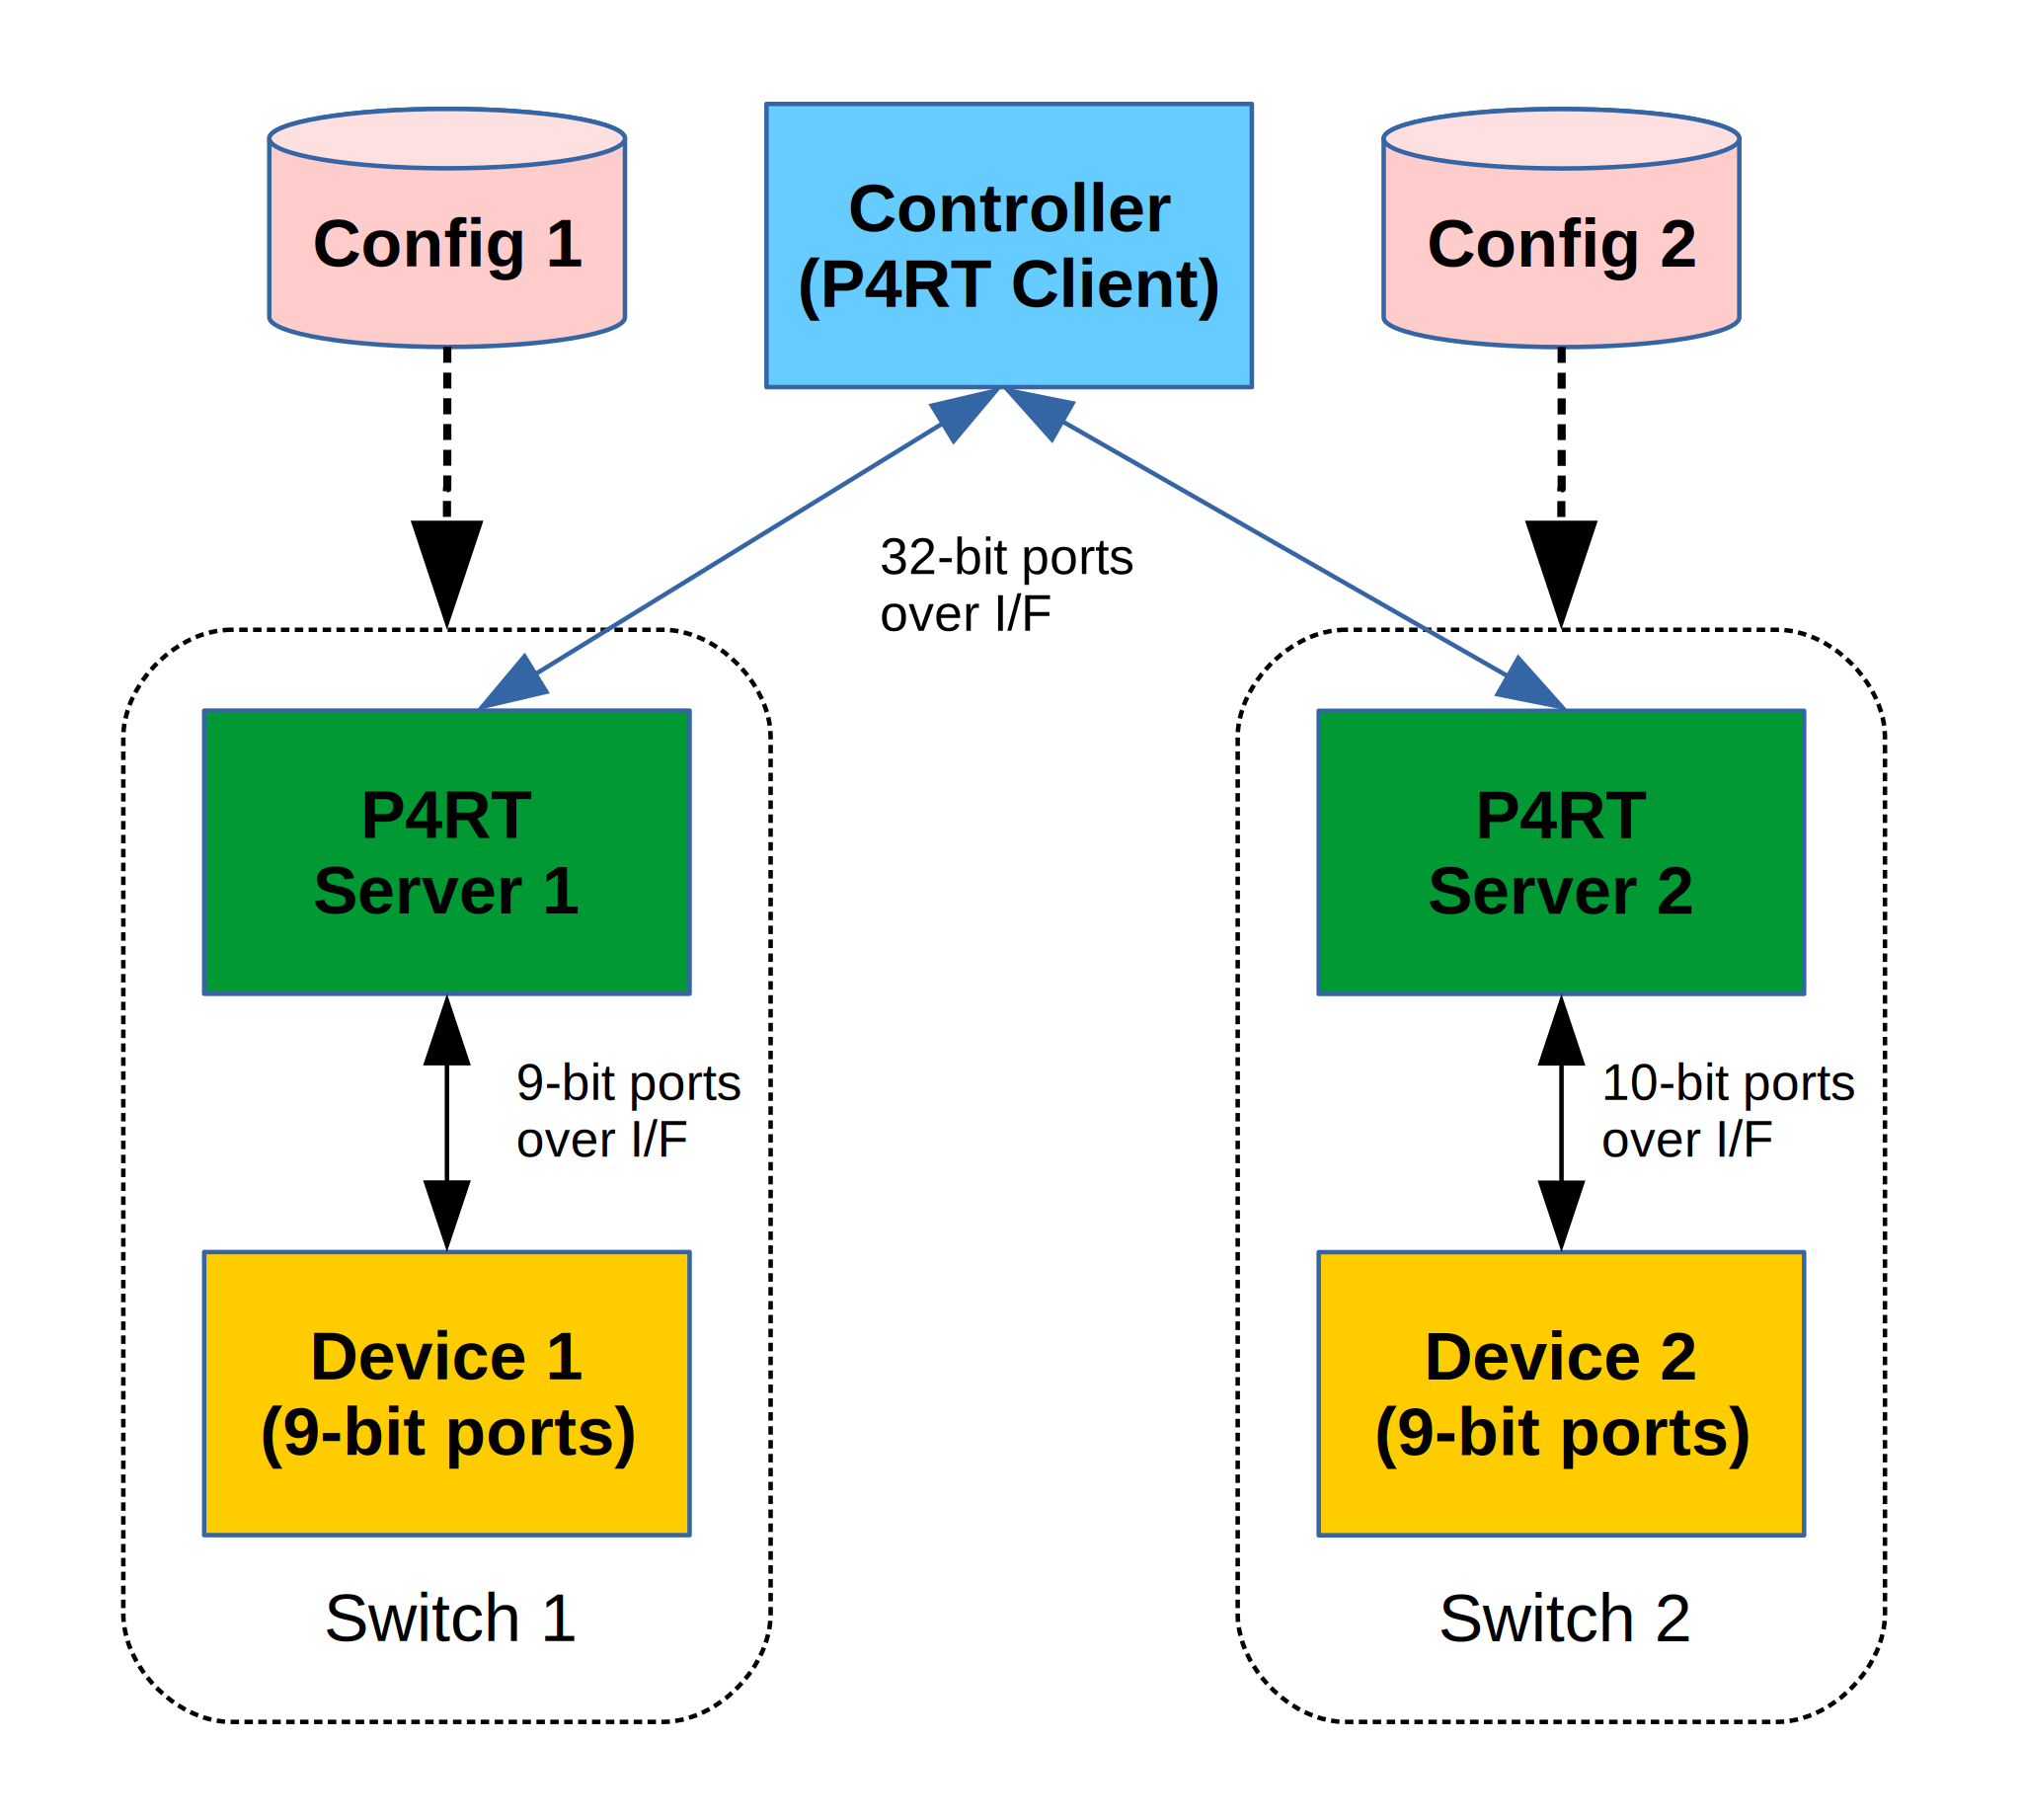
\includegraphics[keepaspectratio=true,height=7cm]{build/psa-metadata-translation}{}\mdline{5186}%mdk

%mdk-data-line={5187}
\mdhr{}%mdk

%mdk-data-line={5188}
\noindent\mdline{5188}\mdcaption{\textbf{Figure~\mdcaptionlabel{8}.}~\mdcaptiontext{P4Runtime Metadata Translation for the Portable Switch Architecture}}%mdk
%mdk
\end{mdcenter}\label{fig-psa-metadata-translation}%mdk
%mdk
\end{figure}%mdk

%mdk-data-line={5192}
\noindent\mdline{5192}Figure\mdline{5192}~\mdref{fig-psa-metadata-translation}{\mdcaptionlabel{8}}\mdline{5192} illustrates a motivating example,
where a centralized controller is controlling two P4Runtime targets in a fabric.
Switch 1 and Switch 2 use different PSA devices, each defining its own port type
and number space. In this example, Switch 1 uses a device with 9-bit space for
port numbers, and Switch 2 uses a device with 10-bit space for port numbers. The
centralized SDN controller defines an independent 32-bit number space for ports
of all targets in its domain. A mapping from the controller\mdline{5198}'\mdline{5198}s 32 bit port
numbers to a target\mdline{5199}'\mdline{5199}s 9-bit or 10-bit port numbers is input to the switch via
the non-forwarding switch config data that is delivered separately to the
switch.%mdk

%mdk-data-line={5203}
\subsubsection{\mdline{5203}17.1.1.\hspace*{0.5em}\mdline{5203}Translation of Port Numbers}\label{sec-translation-of-port-numbers}%mdk%mdk

%mdk-data-line={5205}
\noindent\mdline{5205}In order to support the above SDN use case, P4Runtime requires translation of
port metadata values between the controller\mdline{5206}'\mdline{5206}s space and the PSA device\mdline{5206}'\mdline{5206}s space
as needed. Such translation is enabled by identifying a P4 entity (match field,
action parameter, controller-header field or other) as being a PSA port metadata
type. For this purpose, PSA defines the port metadata field type using special
\mdline{5210}\mdref{sec-user-defined-types}{user-defined P4 types}\mdline{5210}, namely \mdline{5210}\mdcode{{\mdfontfamily{LuxiMono}{\mdfontsize{\dimfont{0.75}}PortId\_t}}}\mdline{5210} and
\mdline{5211}\mdcode{{\mdfontfamily{LuxiMono}{\mdfontsize{\dimfont{0.75}}PortIdInHeader\_t}}}\mdline{5211}, instead of standard P4 bitstrings. The P4Info entries for
all P4 entities whose type is one of the special PSA port types use a
controller-defined 32-bit type instead of the data plane bitwidth defined in the
P4 program. The following PSA port metadata types are defined in \mdline{5214}\emph{psa.p4}\mdline{5214} for
the PSA device in Switch 1.%mdk

%mdk-data-line={5217}
\begin{mdbmargintb}{6pt}{6pt}%mdk
\begin{mdblock}{padding=6pt,border-width=0.5pt,border-style=solid,background-color=\#FFFFDD,breakable=true}%mdk
%mdk-data-line={5218}
\begin{mdpre}%mdk
\noindent{\mdfontfamily{LuxiMono}{\mdfontsize{\dimfont{0.75}}{\mdcolor{gray}@}{\mdcolor{gray}p4runtime\_translation}{\mdcolor{maroon}("p4.org/psa/v1/PortId\_t",~32)}\\
{\bfseries{\mdcolor{navy}type}}~PortId\_t~{\bfseries{\mdcolor{navy}bit}}\textless{}{\mdcolor{purple}9}\textgreater{};\\
{\mdcolor{gray}@}{\mdcolor{gray}p4runtime\_translation}{\mdcolor{maroon}("p4.org/psa/v1/PortIdInHeader\_t",~32)}\\
{\bfseries{\mdcolor{navy}type}}~PortIdInHeader\_t~{\bfseries{\mdcolor{navy}bit}}\textless{}{\mdcolor{purple}32}\textgreater{};}}%mdk
\end{mdpre}%mdk%mdk
\end{mdblock}%mdk
\end{mdbmargintb}%mdk

%mdk-data-line={5224}
\noindent\mdline{5224}The first argument to the \mdline{5224}\mdcode{{\mdfontfamily{LuxiMono}{\mdfontsize{\dimfont{0.75}}@p4runtime\_translation}}}\mdline{5224} annotation is a URI that
indicates to the P4Runtime server which numerical mapping\mdline{5225} \mdline{5225}\textemdash{}\mdline{5225} provided by the
out-of-band switch configuration mechanism\mdline{5226} \mdline{5226}\textemdash{}\mdline{5226} to use to translate between the
SDN value and the data plane value. The second argument is the bitwidth of the
SDN representation of the translated entity (32-bit in the case of ports).%mdk

%mdk-data-line={5230}
\mdline{5230}An SDN port number of 0 is invalid (while 0 may be a valid device port number
depending on the PSA device). A PSA device may define its CPU and recirculation
ports in the device-specific port number space. P4Runtime reserves
device-independent and controller-specific 32-bit constants for the CPU port and
the recirculation port as follows:%mdk

%mdk-data-line={5236}
\begin{mdbmargintb}{6pt}{6pt}%mdk
\begin{mdblock}{padding=6pt,border-width=0.5pt,border-style=solid,background-color=\#E6FFFF,breakable=true}%mdk
%mdk-data-line={5237}
\begin{mdpre}%mdk
\noindent{\mdfontfamily{LuxiMono}{\mdfontsize{\dimfont{0.75}}{\bfseries{\mdcolor{navy}enum}}~SdnPort~\{\\
~~SDN\_PORT\_UNSPECIFIED~{\bfseries{\mdcolor{navy}=}}~{\mdcolor{purple}0};\\
\\
~~{\mdcolor{darkgreen}//~SDN~ports~are~numbered~starting~form~1.}\\
~~SDN\_PORT\_MIN~{\bfseries{\mdcolor{navy}=}}~{\mdcolor{purple}1};\\
\\
~~{\mdcolor{darkgreen}//~The~maximum~value~of~an~SDN~port~(physical~or~logical).}\\
~~SDN\_PORT\_MAX~{\bfseries{\mdcolor{navy}=}}~{\mdcolor{purple}0xfffffeff};\\
\\
~~{\mdcolor{darkgreen}//~Reserved~SDN~port~numbers~(0xfffffff0~-~0xffffffff)}\\
\\
~~SDN\_PORT\_RECIRCULATE~{\bfseries{\mdcolor{navy}=}}~{\mdcolor{purple}0xfffffffa};\\
~~SDN\_PORT\_CPU~{\bfseries{\mdcolor{navy}=}}~{\mdcolor{purple}0xfffffffd};\\
\}}}%mdk
\end{mdpre}%mdk%mdk
\end{mdblock}%mdk
\end{mdbmargintb}%mdk

%mdk-data-line={5253}
\noindent\mdline{5253}The switch config will map \mdline{5253}\mdcode{{\mdfontfamily{LuxiMono}{\mdfontsize{\dimfont{0.75}}SDN\_PORT\_RECIRCULATE}}}\mdline{5253} and \mdline{5253}\mdcode{{\mdfontfamily{LuxiMono}{\mdfontsize{\dimfont{0.75}}SDN\_PORT\_CPU}}}\mdline{5253} \mdline{5253}\textemdash{}\mdline{5253} as well
as any SDN port number corresponding to a \mdline{5254}\textquotedblleft{}regular\textquotedblright{}\mdline{5254} front-panel port\mdline{5254} \mdline{5254}\textemdash{}\mdline{5254} to the
corresponding device-specific values, in order to enable the P4Runtime server to
perform the translation.%mdk

%mdk-data-line={5258}
\mdline{5258}The sub-sections below detail the translation mechanics for different usage of
PSA port types in P4 programs.%mdk

%mdk-data-line={5261}
\subsubsection{\mdline{5261}17.1.2.\hspace*{0.5em}\mdline{5261}Translation of Packet-IO Header Fields}\label{sec-translation-of-packet-io-header-fields}%mdk%mdk

%mdk-data-line={5263}
\noindent\mdline{5263}Port type fields can be part of header types. For example, ports may be part of
Packet IO headers, as in the following example:.%mdk

%mdk-data-line={5266}
\begin{mdbmargintb}{6pt}{6pt}%mdk
\begin{mdblock}{padding=6pt,border-width=0.5pt,border-style=solid,background-color=\#FFFFDD,breakable=true}%mdk
%mdk-data-line={5267}
\begin{mdpre}%mdk
\noindent{\mdfontfamily{LuxiMono}{\mdfontsize{\dimfont{0.75}}{\mdcolor{gray}@}{\mdcolor{gray}controller\_header}{\mdcolor{maroon}("packet\_out")}\\
{\bfseries{\mdcolor{navy}header}}~PacketOut\_t~\{\\
~~PortIdInHeader\_t~egress\_port;\\
\}\\
\\
{\mdcolor{gray}@}{\mdcolor{gray}controller\_header}{\mdcolor{maroon}("packet\_in")}\\
{\bfseries{\mdcolor{navy}header}}~PacketIn\_t~\{\\
~~PortIdInHeader\_t~ingress\_port;\\
\}}}%mdk
\end{mdpre}%mdk%mdk
\end{mdblock}%mdk
\end{mdbmargintb}%mdk

%mdk-data-line={5278}
\noindent\mdline{5278}The header-level annotation \mdline{5278}\mdcode{{\mdfontfamily{LuxiMono}{\mdfontsize{\dimfont{0.75}}@controller\_header}}}\mdline{5278} is a standard P4Runtime
annotation that identifies a header type for a controller packet-out or
packet-in header. When the P4Runtime server in the target receives a packet-out
from the controller over the P4Runtime stream channel, the server will expect a
packet-out metadata (\mdline{5282}\mdcode{{\mdfontfamily{LuxiMono}{\mdfontsize{\dimfont{0.75}}egress\_port}}}\mdline{5282}) value of width 32-bit from the given set of
SDN port values in the switch config. The server will then translate the SDN
port value into the device-specific port value from the mapping provided in the
out-of-band switch configuration (the mapping can be identified using the
translation URI\mdline{5286} \mdline{5286}\textemdash{}\mdline{5286} first argument to the \mdline{5286}\mdcode{{\mdfontfamily{LuxiMono}{\mdfontsize{\dimfont{0.75}}@p4runtime\_translation}}}\mdline{5286}
annotation). Any subsequent reference to the \mdline{5287}\mdcode{{\mdfontfamily{LuxiMono}{\mdfontsize{\dimfont{0.75}}egress\_port}}}\mdline{5287} field in the
data plane will use the translated value. \mdline{5288}\mdcode{{\mdfontfamily{LuxiMono}{\mdfontsize{\dimfont{0.75}}PortIdInHeader\_t}}}\mdline{5288} is used in the
header definition instead of \mdline{5289}\mdcode{{\mdfontfamily{LuxiMono}{\mdfontsize{\dimfont{0.75}}PortId\_t}}}\mdline{5289} to guarantee byte-aligned headers in
case this is required by the target.%mdk

%mdk-data-line={5292}
\mdline{5292}A similar reverse translation is required in the P4Runtime server for packets
punted from the target to the controller as shown by the packet-in header
example above. A packet punted from the target\mdline{5294}'\mdline{5294}s PSA device will be intercepted
by the P4Runtime server before being sent to the controller. The server will
first translate the device-specific value of the \mdline{5296}\mdcode{{\mdfontfamily{LuxiMono}{\mdfontsize{\dimfont{0.75}}ingress\_port}}}\mdline{5296} field into the
controller-specific 32-bit value given by the port mapping defined in the switch
config. The server will then insert the translated controller-specific value in
the packet-in metadata fields before sending the packet over the stream channel
to the controller.%mdk

%mdk-data-line={5302}
\subsubsection{\mdline{5302}17.1.3.\hspace*{0.5em}\mdline{5302}Translation of Match Fields}\label{sec-translation-of-match-fields}%mdk%mdk

%mdk-data-line={5304}
\noindent\mdline{5304}Port type entities, particularly ingress and egress port standard metadata, may
be used as match fields in a P4 table\mdline{5305}'\mdline{5305}s match key as shown in the example below:%mdk

%mdk-data-line={5307}
\begin{mdbmargintb}{6pt}{6pt}%mdk
\begin{mdblock}{padding=6pt,border-width=0.5pt,border-style=solid,background-color=\#FFFFDD,breakable=true}%mdk
%mdk-data-line={5308}
\begin{mdpre}%mdk
\noindent{\mdfontfamily{LuxiMono}{\mdfontsize{\dimfont{0.75}}{\bfseries{\mdcolor{navy}table}}~t~\{\\
~~key~=~\{\\
~~~~istd.ingress\_port:~exact;~~{\mdcolor{darkgreen}//~PSA~standard~metadata~ingress~port}\\
~~\}\\
~~actions~=~\{\\
~~~~drop;\\
~~\}\\
\}}}%mdk
\end{mdpre}%mdk%mdk
\end{mdblock}%mdk
\end{mdbmargintb}%mdk

%mdk-data-line={5318}
\noindent\mdline{5318}Table \mdline{5318}\mdcode{{\mdfontfamily{LuxiMono}{\mdfontsize{\dimfont{0.75}}t}}}\mdline{5318} has an exact match on PSA standard metadata ingress port
(\mdline{5319}\mdcode{{\mdfontfamily{LuxiMono}{\mdfontsize{\dimfont{0.75}}istd.ingress\_port}}}\mdline{5319}). Since the field is of type \mdline{5319}\mdcode{{\mdfontfamily{LuxiMono}{\mdfontsize{\dimfont{0.75}}PortId\_t}}}\mdline{5319}, the P4Info
representation of the match field will present a 32-bit bitwidth to the
controller, regardless of the data plane port type. A P4Runtime write request
for a table entry in \mdline{5322}\mdcode{{\mdfontfamily{LuxiMono}{\mdfontsize{\dimfont{0.75}}t}}}\mdline{5322} from the controller will have the values of the match
field set to the controller-specific port value. The P4Runtime server should
intercept the write request and use the switch configuration data to translate
the SDN port value to respective device-specific value. In the data plane, the
packet metadata will carry the device-specific value and, hence, match the right
table entry. Similarly, when a read response for table \mdline{5327}\mdcode{{\mdfontfamily{LuxiMono}{\mdfontsize{\dimfont{0.75}}t}}}\mdline{5327} is returned to the
controller, the P4Runtime server should translate the device-specific port
values to the corresponding controller-specific values.%mdk

%mdk-data-line={5331}
\mdline{5331}Note that it may be infeasible to translate the value-mask pair for ternary
matches: \mdline{5332}\mdcode{{\mdfontfamily{LuxiMono}{\mdfontsize{\dimfont{0.75}}LPM}}}\mdline{5332}, \mdline{5332}\mdcode{{\mdfontfamily{LuxiMono}{\mdfontsize{\dimfont{0.75}}TERNARY}}}\mdline{5332} or \mdline{5332}\mdcode{{\mdfontfamily{LuxiMono}{\mdfontsize{\dimfont{0.75}}RANGE}}}\mdline{5332} match kinds.  The P4Runtime server may
require that for these match kinds the port match be either \mdline{5333}\emph{de facto}\mdline{5333} \mdline{5333}\textquotedblleft{}exact\textquotedblright{}\mdline{5333}
(0xffffffff mask for \mdline{5334}\mdcode{{\mdfontfamily{LuxiMono}{\mdfontsize{\dimfont{0.75}}TERNARY}}}\mdline{5334}, prefix-length of 32 for \mdline{5334}\mdcode{{\mdfontfamily{LuxiMono}{\mdfontsize{\dimfont{0.75}}LPM}}}\mdline{5334}, or same low and
high bounds for \mdline{5335}\mdcode{{\mdfontfamily{LuxiMono}{\mdfontsize{\dimfont{0.75}}RANGE}}}\mdline{5335}) or \mdline{5335}\textquotedblleft{}don't care\textquotedblright{}\mdline{5335}.%mdk

%mdk-data-line={5337}
\subsubsection{\mdline{5337}17.1.4.\hspace*{0.5em}\mdline{5337}Translation of Action Parameters}\label{sec-translation-of-action-parameters}%mdk%mdk

%mdk-data-line={5339}
\noindent\mdline{5339}\mdcode{{\mdfontfamily{LuxiMono}{\mdfontsize{\dimfont{0.75}}PortId\_t}}}\mdline{5339} type parameters can be part of a P4 action definition as shown in the
example below:%mdk

%mdk-data-line={5342}
\begin{mdbmargintb}{6pt}{6pt}%mdk
\begin{mdblock}{padding=6pt,border-width=0.5pt,border-style=solid,background-color=\#FFFFDD,breakable=true}%mdk
%mdk-data-line={5343}
\begin{mdpre}%mdk
\noindent{\mdfontfamily{LuxiMono}{\mdfontsize{\dimfont{0.75}}{\bfseries{\mdcolor{navy}action}}~a(PortId\_t~p)~\{\\
~~istd.egress\_port~=~p;~~{\mdcolor{darkgreen}//~PSA~standard~metadata~egress~port}\\
\}\\
\\
{\bfseries{\mdcolor{navy}table}}~t~\{\\
~~key~=~\{\\
~~~~hdr.h.f:~exact;\\
~~\}\\
~~actions~=~\{\\
~~~~a;\\
~~\}\\
\}}}%mdk
\end{mdpre}%mdk%mdk
\end{mdblock}%mdk
\end{mdbmargintb}%mdk

%mdk-data-line={5357}
\noindent\mdline{5357}The controller may write entries in table \mdline{5357}\mdcode{{\mdfontfamily{LuxiMono}{\mdfontsize{\dimfont{0.75}}t}}}\mdline{5357} with action \mdline{5357}\mdcode{{\mdfontfamily{LuxiMono}{\mdfontsize{\dimfont{0.75}}a}}}\mdline{5357} to set the egress
port as shown in the P4 code above. The action parameter \mdline{5358}\mdcode{{\mdfontfamily{LuxiMono}{\mdfontsize{\dimfont{0.75}}p}}}\mdline{5358} is of type
\mdline{5359}\mdcode{{\mdfontfamily{LuxiMono}{\mdfontsize{\dimfont{0.75}}PortId\_t}}}\mdline{5359}, which leads to a 32-bit bitwidth for \mdline{5359}\mdcode{{\mdfontfamily{LuxiMono}{\mdfontsize{\dimfont{0.75}}p}}}\mdline{5359} being exposed in
P4Info. Furthermore, the type will be a signal to the P4Runtime server that
translation is required for this parameter. The P4Runtime server will use the
switch configuration to translate action parameter values between the controller
and the target device.%mdk

%mdk-data-line={5365}
\subsubsection{\mdline{5365}17.1.5.\hspace*{0.5em}\mdline{5365}Port Translation for PSA Extern APIs}\label{sec-port-translation-for-psa-extern-apis}%mdk%mdk

%mdk-data-line={5367}
\noindent\mdline{5367}The P4Runtime API for action selectors supports specifying a watch field per
member in an action profile group that is programmed in a selector. This field
is used to implement fast-failover in the target, where the P4Runtime server can
locally prune the member from the group if a port is down. This pruning does not
require intervention from the controller. Conversely, if the port comes back up,
the P4Runtime server can re-enable the member in the group. The watch field is
of type \mdline{5373}\mdcode{{\mdfontfamily{LuxiMono}{\mdfontsize{\dimfont{0.75}}uint32}}}\mdline{5373} to carry the 32-bit SDN representation of the port being
watched. The P4Runtime server will translate the given watch port number into
the device-specific data plane port number for implementing the fast-failover
functionality on the target device.%mdk

%mdk-data-line={5378}
\mdline{5378}The Packet Replication Engine (PRE) API in P4Runtime supports cloning and
multicasting to a set of ports. The egress port fields defined in the PRE
multicast entry and clone session entry are of type \mdline{5380}\mdcode{{\mdfontfamily{LuxiMono}{\mdfontsize{\dimfont{0.75}}uint32}}}\mdline{5380} to carry the 32-bit
SDN port number(s). The P4Runtime server will translate these SDN port numbers
to device-specific port numbers for multicasting and cloning in the data plane.%mdk

%mdk-data-line={5384}
\subsubsection{\mdline{5384}17.1.6.\hspace*{0.5em}\mdline{5384}Using Port as an Index to a Register, Indirect Counter or Indirect Meter}\label{sec-using-port-as-an-index-to-a-register-indirect-counter-or-indirect-meter}%mdk%mdk

%mdk-data-line={5386}
\noindent\mdline{5386}P4Runtime supports using a translated value (\mdline{5386}\mdcode{{\mdfontfamily{LuxiMono}{\mdfontsize{\dimfont{0.75}}PortId\_t}}}\mdline{5386} or any other translated
type for which the underlying built-in type is \mdline{5387}\mdcode{{\mdfontfamily{LuxiMono}{\mdfontsize{\dimfont{0.75}}bit\textless{}W\textgreater{}}}}\mdline{5387}) as an index to a
register, indirect counter, or indirect meter.%mdk

%mdk-data-line={5390}
\begin{mdbmargintb}{6pt}{6pt}%mdk
\begin{mdblock}{padding=6pt,border-width=0.5pt,border-style=solid,background-color=\#FFFFDD,breakable=true}%mdk
%mdk-data-line={5391}
\begin{mdpre}%mdk
\noindent{\mdfontfamily{LuxiMono}{\mdfontsize{\dimfont{0.75}}Counter\textless{}{\bfseries{\mdcolor{navy}bit}}\textless{}{\mdcolor{purple}32}\textgreater{}~{\mdcolor{darkgreen}/*}{\mdcolor{darkgreen}~counter~entry~type~}{\mdcolor{darkgreen}*/},~PortId\_t~{\mdcolor{darkgreen}/*}{\mdcolor{darkgreen}~index~type~}{\mdcolor{darkgreen}*/}\textgreater{}(\\
~~{\mdcolor{purple}32}w1024,~PSA\_CounterType\_t.PACKETS)~counter;\\
{\bfseries{\mdcolor{navy}action}}~a(PortId\_t~p)~\{\\
~~istd.egress\_port~=~p;~~{\mdcolor{darkgreen}//~PSA~standard~metadata~egress~port}\\
~~counter.count(p);\\
\}}}%mdk
\end{mdpre}%mdk%mdk
\end{mdblock}%mdk
\end{mdbmargintb}%mdk

%mdk-data-line={5399}
\noindent\mdline{5399}This P4 Counter declaration will translate into the following entry in the
P4Info messsage:%mdk

%mdk-data-line={5402}
\begin{mdbmargintb}{6pt}{6pt}%mdk
\begin{mdblock}{padding=6pt,border-width=0.5pt,border-style=solid,background-color=\#E6FFFF,breakable=true}%mdk
%mdk-data-line={5403}
\begin{mdpre}%mdk
\noindent{\mdfontfamily{LuxiMono}{\mdfontsize{\dimfont{0.75}}counters~\{\\
~~preamble~\{\\
~~~~id:~{\mdcolor{purple}0x12000001}\\
~~~~name:~{\mdcolor{maroon}"}{\mdcolor{maroon}counter}{\mdcolor{maroon}"}\\
~~\}\\
~~spec~\{\\
~~~~unit:~PACKETS\\
~~\}\\
~~index\_type\_name~\{\\
~~~~name:~{\mdcolor{maroon}"}{\mdcolor{maroon}PortId\_t}{\mdcolor{maroon}"}\\
~~\}\\
\}}}%mdk
\end{mdpre}%mdk%mdk
\end{mdblock}%mdk
\end{mdbmargintb}%mdk

%mdk-data-line={5417}
\noindent\mdline{5417}The controller may read and write counter values from indexed counter \mdline{5417}\mdcode{{\mdfontfamily{LuxiMono}{\mdfontsize{\dimfont{0.75}}counter}}}\mdline{5417}
using SDN port numbers as indices, and not device-specific port numbers. The
\mdline{5419}\mdcode{{\mdfontfamily{LuxiMono}{\mdfontsize{\dimfont{0.75}}index\_type\_name}}}\mdline{5419} field in the P4Info message is a signal to the P4Runtime
server that translation is required.%mdk

%mdk-data-line={5422}
\section{\mdline{5422}18.\hspace*{0.5em}\mdline{5422}P4Runtime Versioning}\label{sec-p4runtime-versioning}%mdk%mdk

%mdk-data-line={5424}
\noindent\mdline{5424}P4Runtime follows the Google guidelines for versioning cloud APIs
\mdline{5425}[\mdcite{apiversioning}{6}]\mdline{5425}. We use a \mdline{5425}\mdcode{{\mdfontfamily{LuxiMono}{\mdfontsize{\dimfont{0.75}}MAJOR.MINOR.PATCH}}}\mdline{5425} style version number scheme and
we increment the:%mdk

%mdk-data-line={5428}
\begin{itemize}[noitemsep,topsep=\mdcompacttopsep]%mdk

%mdk-data-line={5428}
\item\mdline{5428}\mdcode{{\mdfontfamily{LuxiMono}{\mdfontsize{\dimfont{0.75}}MAJOR}}}\mdline{5428} version when we make incompatible API changes,%mdk

%mdk-data-line={5429}
\item\mdline{5429}\mdcode{{\mdfontfamily{LuxiMono}{\mdfontsize{\dimfont{0.75}}MINOR}}}\mdline{5429} version when we add functionality in a backwards-compatible manner,%mdk

%mdk-data-line={5430}
\item\mdline{5430}\mdcode{{\mdfontfamily{LuxiMono}{\mdfontsize{\dimfont{0.75}}PATCH}}}\mdline{5430} version when we make backwards-compatible bug fixes.%mdk
%mdk
\end{itemize}%mdk

%mdk-data-line={5432}
\noindent\mdline{5432}The major version number is encoded as the last component of the Protobuf
package name for every P4Runtime version, including version 1 (v1), which is why
currently the package name for the P4Runtime service is \mdline{5434}\mdcode{{\mdfontfamily{LuxiMono}{\mdfontsize{\dimfont{0.75}}p4.v1}}}\mdline{5434} and the package
name for P4Info is \mdline{5435}\mdcode{{\mdfontfamily{LuxiMono}{\mdfontsize{\dimfont{0.75}}p4.config.v1}}}\mdline{5435}. Even though \mdline{5435}\mdcode{{\mdfontfamily{LuxiMono}{\mdfontsize{\dimfont{0.75}}p4}}}\mdline{5435} and \mdline{5435}\mdcode{{\mdfontfamily{LuxiMono}{\mdfontsize{\dimfont{0.75}}p4.config}}}\mdline{5435} are two
different Protobuf packages, \mdline{5436}\mdcode{{\mdfontfamily{LuxiMono}{\mdfontsize{\dimfont{0.75}}p4}}}\mdline{5436} depends on \mdline{5436}\mdcode{{\mdfontfamily{LuxiMono}{\mdfontsize{\dimfont{0.75}}p4.config}}}\mdline{5436} and is not meant to be
used without it, which is why both packages use the same versioning scheme and
the same versioning cadence.%mdk

%mdk-data-line={5440}
\mdline{5440}As recommended in\mdline{5440}~[\mdcite{apiversioning}{6}]\mdline{5440}, we may consider using pre-GA release
suffixes (such as \mdline{5441}\emph{alpha}\mdline{5441} or \mdline{5441}\emph{beta}\mdline{5441}) in the Protobuf package name for future
major versions, although we have chosen not to do so when developing version 1
(v1).%mdk

%mdk-data-line={5445}
\mdline{5445}Within a major version, the API must be evolved in a Protobuf
backwards-compatible manner.\mdline{5446}~[\mdcite{apiversioningbackwardscompatibility}{7}]\mdline{5446} describes
what constitute a backwards-compatible change. We expect \mdline{5447}\mdcode{{\mdfontfamily{LuxiMono}{\mdfontsize{\dimfont{0.75}}MAJOR}}}\mdline{5447} version bumps
to be a \mdline{5448}\textbf{rare}\mdline{5448} event.%mdk

%mdk-data-line={5450}
\mdline{5450}Note that a P4Runtime server may support multiple major versions of P4Runtime,
although a client is expected to use the same version of the P4Runtime service
for all its operations with a given device, during the lifetime of its session
with the device. A client can check if a major version is supported by
attempting to connect to the corresponding service. We may consider including a
P4Runtime RPC to query minor\mdline{5455} \mdline{5455}+ patch version numbers in future releases.%mdk

%mdk-data-line={5457}
\mdline{5457}All versions of P4Runtime, including pre-release versions, are tagged in the
P4Runtime Github repository\mdline{5458}~[\mdcite{p4runtimerepo}{14}]\mdline{5458} and the version label follows
semantic versioning rules\mdline{5459}~[\mdcite{semver}{26}]\mdline{5459}.%mdk

%mdk-data-line={5461}
\section{\mdline{5461}19.\hspace*{0.5em}\mdline{5461}Extending P4Runtime for non-PSA Architectures}\label{sec-extending-p4runtime}%mdk%mdk

%mdk-data-line={5463}
\noindent\mdline{5463}P4Runtime includes native support for PSA programs and in particular support for
runtime control of PSA extern instances. While the definition of Protobuf
messages for runtime control of non-PSA externs is out-of-scope of this
specification, P4Runtime provides an extension mechanism for other
architectures, through different hooks in the protocol definition. These hooks
are described in various parts of this document and the goal of this section is
to offer a comprehensive list of them in a single place.%mdk

%mdk-data-line={5471}
\mdline{5471}When extending P4Runtime for a new P4 architecture, one will need to write two
additional Protobuf files to extend p4info.proto and p4runtime.proto
respectively. We suggest the following Protobuf package names:%mdk

%mdk-data-line={5475}
\begin{itemize}[noitemsep,topsep=\mdcompacttopsep]%mdk

%mdk-data-line={5475}
\item\mdline{5475}\mdcode{{\mdfontfamily{LuxiMono}{\mdfontsize{\dimfont{0.75}}p4/{}[organization]/arch/config/\textless{}major~version\textgreater{}/p4info.proto}}}\mdline{5475}%mdk

%mdk-data-line={5476}
\item\mdline{5476}\mdcode{{\mdfontfamily{LuxiMono}{\mdfontsize{\dimfont{0.75}}p4/{}[organization]/arch/\textless{}major~version\textgreater{}/p4runtime.proto}}}\mdline{5476}%mdk
%mdk
\end{itemize}%mdk

%mdk-data-line={5478}
\noindent\mdline{5478}We also recommend that the major version number for these packages be the same
as the major version number for the P4Runtime version they \mdline{5479}\textquotedblleft{}extend\textquotedblright{}\mdline{5479}.%mdk

%mdk-data-line={5481}
\mdline{5481}For the remainder of this section, we will refer to these two files as
\mdline{5482}\emph{p4info-ext}\mdline{5482} and \mdline{5482}\emph{p4runtime-ext}\mdline{5482} respectively.%mdk

%mdk-data-line={5484}
\subsection{\mdline{5484}19.1.\hspace*{0.5em}\mdline{5484}Extending P4Runtime for Architecture-Specific Externs}\label{sec-extending-p4runtime-for-architecture-specific-externs}%mdk%mdk

%mdk-data-line={5486}
\noindent\mdline{5486}Each P4 architecture can define its own set of extern types. Controlling them at
runtime requires defining new Protobuf messages in both \mdline{5487}\emph{p4info-ext}\mdline{5487} and
\mdline{5488}\emph{p4runtime-ext}\mdline{5488}. To make things more concrete for this section, we will assume
that the new architecture we are trying to support in P4Runtime includes the
following extern definition, which we will use as a running example:%mdk

%mdk-data-line={5492}
\begin{mdbmargintb}{6pt}{6pt}%mdk
\begin{mdblock}{padding=6pt,border-width=0.5pt,border-style=solid,background-color=\#FFFFDD,breakable=true}%mdk
%mdk-data-line={5493}
\begin{mdpre}%mdk
\noindent{\mdfontfamily{LuxiMono}{\mdfontsize{\dimfont{0.75}}{\mdcolor{darkgreen}//~T~must~be~a~bit\textless{}W\textgreater{}~type,~it~indicates~the~width~of~each~counter~cell}\\
{\bfseries{\mdcolor{navy}extern}}~MyNewPacketCounter\textless{}T\textgreater{}~\{\\
~~counter({\bfseries{\mdcolor{navy}bit}}\textless{}{\mdcolor{purple}32}\textgreater{}~size);\\
~~increment({\bfseries{\mdcolor{navy}in}}~{\bfseries{\mdcolor{navy}bit}}\textless{}{\mdcolor{purple}32}\textgreater{}~index);\\
\}}}%mdk
\end{mdpre}%mdk%mdk
\end{mdblock}%mdk
\end{mdbmargintb}%mdk

%mdk-data-line={5500}
\subsubsection{\mdline{5500}19.1.1.\hspace*{0.5em}\mdline{5500}Extending the P4Info message}\label{sec-extending-the-p4info-message}%mdk%mdk

%mdk-data-line={5502}
\begin{itemize}[noitemsep,topsep=\mdcompacttopsep]%mdk

%mdk-data-line={5502}
\item\mdline{5502}Id prefixes \mdline{5502}\mdcode{{\mdfontfamily{LuxiMono}{\mdfontsize{\dimfont{0.75}}0x81}}}\mdline{5502} through \mdline{5502}\mdcode{{\mdfontfamily{LuxiMono}{\mdfontsize{\dimfont{0.75}}0xfe}}}\mdline{5502} are reserved for architecture-specific
externs. It is recommended that \mdline{5503}\emph{p4info-ext}\mdline{5503} include a \mdline{5503}\mdcode{{\mdfontfamily{LuxiMono}{\mdfontsize{\dimfont{0.75}}P4Ids}}}\mdline{5503} message based
on the one in p4info.proto that the P4 compiler can refer to when\mdline{5504}~\mdref{sec-id-allocation}{assigning
IDs}\mdline{5505} to each extern instance.%mdk
%mdk
\end{itemize}%mdk

%mdk-data-line={5507}
\begin{mdbmargintb}{6pt}{6pt}%mdk
\begin{mdblock}{padding=6pt,border-width=0.5pt,border-style=solid,background-color=\#E6FFFF,breakable=true}%mdk
%mdk-data-line={5508}
\begin{mdpre}%mdk
\noindent{\mdfontfamily{LuxiMono}{\mdfontsize{\dimfont{0.75}}{\bfseries{\mdcolor{navy}message}}~P{\mdcolor{purple}4}Ids~\{\\
~~{\bfseries{\mdcolor{navy}enum}}~Prefix~\{\\
~~~~UNSPECIFIED~{\bfseries{\mdcolor{navy}=}}~{\mdcolor{purple}0};\\
~~~~MY\_NEW\_PACKET\_COUNTER~{\bfseries{\mdcolor{navy}=}}~{\mdcolor{purple}0x81};\\
~~\}\\
\}}}%mdk
\end{mdpre}%mdk%mdk
\end{mdblock}%mdk
\end{mdbmargintb}%mdk

%mdk-data-line={5516}
\begin{itemize}[noitemsep,topsep=\mdcompacttopsep]%mdk

%mdk-data-line={5516}
\item\mdline{5516}\emph{p4info-ext}\mdline{5516} should include a Protobuf message definition for every extern
type that can be controlled at runtime. For every extern instance of this
type, the compiler will generate an instance of this Protobuf message and
embed it appropriately in the corresponding
\mdline{5520}\mdref{sec-p4info-extern}{\mdcode{{\mdfontfamily{LuxiMono}{\mdfontsize{\dimfont{0.75}}p4.config.v1.ExternInstance}}}}\mdline{5520} message as the \mdline{5520}\mdcode{{\mdfontfamily{LuxiMono}{\mdfontsize{\dimfont{0.75}}info}}}\mdline{5520}
field, which is of type \mdline{5521}\mdcode{{\mdfontfamily{LuxiMono}{\mdfontsize{\dimfont{0.75}}Any}}}\mdline{5521}~[\mdcite{protoany}{29}]\mdline{5521}.%mdk
%mdk
\end{itemize}%mdk

%mdk-data-line={5523}
\begin{mdbmargintb}{6pt}{6pt}%mdk
\begin{mdblock}{padding=6pt,border-width=0.5pt,border-style=solid,background-color=\#E6FFFF,breakable=true}%mdk
%mdk-data-line={5524}
\begin{mdpre}%mdk
\noindent{\mdfontfamily{LuxiMono}{\mdfontsize{\dimfont{0.75}}{\bfseries{\mdcolor{navy}message}}~MyNewPacketCounter~\{\\
~~{\mdcolor{darkgreen}//~corresponds~to~the~T~type~parameter~in~the~P4~extern~definition}\\
~~p4.config.v1.P{\mdcolor{purple}4}DataTypeSpec~type\_spec~{\bfseries{\mdcolor{navy}=}}~{\mdcolor{purple}1};\\
~~{\mdcolor{darkgreen}//~constructor~argument}\\
~~{\bfseries{\mdcolor{navy}int64}}~size~{\bfseries{\mdcolor{navy}=}}~{\mdcolor{purple}2};\\
\}}}%mdk
\end{mdpre}%mdk%mdk
\end{mdblock}%mdk
\end{mdbmargintb}%mdk

%mdk-data-line={5532}
\subsubsection{\mdline{5532}19.1.2.\hspace*{0.5em}\mdline{5532}Extending the P4Runtime Service}\label{sec-extending-the-p4runtime-service}%mdk%mdk

%mdk-data-line={5534}
\noindent\mdline{5534}Just like \mdline{5534}\emph{p4info-ext}\mdline{5534}, \mdline{5534}\emph{p4runtime-ext}\mdline{5534} should include a Protobuf message
definition for every extern type that can be controlled at runtime. This message
should include the extern-specific parameters defining the read or write
operation to be performed by the P4Runtime server on the corresponding extern
instance. Instances of this architecture-specific message are meant to be
embedded in an\mdline{5539}~\mdref{sec-extern-entry}{\mdcode{{\mdfontfamily{LuxiMono}{\mdfontsize{\dimfont{0.75}}ExternEntry}}}}\mdline{5539} message generated by the
P4Runtime client.%mdk

%mdk-data-line={5542}
\mdline{5542}Here is a possible Protobuf message for our \mdline{5542}\mdcode{{\mdfontfamily{LuxiMono}{\mdfontsize{\dimfont{0.75}}MyNewPacketCounter}}}\mdline{5542} P4 extern:%mdk

%mdk-data-line={5543}
\begin{mdbmargintb}{6pt}{6pt}%mdk
\begin{mdblock}{padding=6pt,border-width=0.5pt,border-style=solid,background-color=\#E6FFFF,breakable=true}%mdk
%mdk-data-line={5544}
\begin{mdpre}%mdk
\noindent{\mdfontfamily{LuxiMono}{\mdfontsize{\dimfont{0.75}}{\mdcolor{darkgreen}//~This~message~enables~reading~/~writing~data~to~the~counter~at~the~provided}\\
{\mdcolor{darkgreen}//~index}\\
{\bfseries{\mdcolor{navy}message}}~MyNewPacketCounter~\{\\
~~{\bfseries{\mdcolor{navy}int64}}~index~{\bfseries{\mdcolor{navy}=}}~{\mdcolor{purple}1};\\
~~p4.v1.P{\mdcolor{purple}4}Data~data~{\bfseries{\mdcolor{navy}=}}~{\mdcolor{purple}2};\\
\}}}%mdk
\end{mdpre}%mdk%mdk
\end{mdblock}%mdk
\end{mdbmargintb}%mdk

%mdk-data-line={5552}
\noindent\mdline{5552}P4Runtime also supports streaming arbitrary Protobuf messages between the server
and the client, by including an \mdline{5553}\mdcode{{\mdfontfamily{LuxiMono}{\mdfontsize{\dimfont{0.75}}Any}}}\mdline{5553} Protobuf field\mdline{5553}~[\mdcite{protoany}{29}]\mdline{5553} named \mdline{5553}\mdcode{{\mdfontfamily{LuxiMono}{\mdfontsize{\dimfont{0.75}}other}}}\mdline{5553}
in both \mdline{5554}\mdcode{{\mdfontfamily{LuxiMono}{\mdfontsize{\dimfont{0.75}}p4.v1.StreamMessageRequest}}}\mdline{5554} and
\mdline{5555}\mdcode{{\mdfontfamily{LuxiMono}{\mdfontsize{\dimfont{0.75}}p4.v1.StreamMessageResponse}}}\mdline{5555}. Architectures that wish to leverage this support
should define the appropriate Protobuf messages for this bidirectional streaming
in \mdline{5557}\emph{p4runtime-ext}\mdline{5557} and embed instances of these messages in
\mdline{5558}\mdcode{{\mdfontfamily{LuxiMono}{\mdfontsize{\dimfont{0.75}}p4.v1.StreamMessageRequest}}}\mdline{5558} and \mdline{5558}\mdcode{{\mdfontfamily{LuxiMono}{\mdfontsize{\dimfont{0.75}}p4.v1.StreamMessageResponse}}}\mdline{5558} as appropriate.%mdk

%mdk-data-line={5560}
\subsection{\mdline{5560}19.2.\hspace*{0.5em}\mdline{5560}Architecture-Specific Table Extensions}\label{sec-architecture-specific-table-extensions}%mdk%mdk

%mdk-data-line={5562}
\subsubsection{\mdline{5562}19.2.1.\hspace*{0.5em}\mdline{5562}New Match Types}\label{sec-new-match-types}%mdk%mdk

%mdk-data-line={5564}
\noindent\mdline{5564}An architecture may introduce new table match types\mdline{5564}~[\mdcite{p4matchtypes}{12}]\mdline{5564}. P4Runtime
accounts for this by providing the following hooks:%mdk

%mdk-data-line={5567}
\begin{itemize}%mdk

%mdk-data-line={5567}
\item{}
%mdk-data-line={5567}
\mdline{5567}The \mdline{5567}\mdcode{{\mdfontfamily{LuxiMono}{\mdfontsize{\dimfont{0.75}}match}}}\mdline{5567} field in \mdline{5567}\mdcode{{\mdfontfamily{LuxiMono}{\mdfontsize{\dimfont{0.75}}p4.config.v1.MatchField}}}\mdline{5567} (p4info.proto) is a \mdline{5567}\mdcode{{\mdfontfamily{LuxiMono}{\mdfontsize{\dimfont{0.75}}oneof}}}\mdline{5567}
which can be either one of the default match types (\mdline{5568}\mdcode{{\mdfontfamily{LuxiMono}{\mdfontsize{\dimfont{0.75}}EXACT}}}\mdline{5568}, \mdline{5568}\mdcode{{\mdfontfamily{LuxiMono}{\mdfontsize{\dimfont{0.75}}LPM}}}\mdline{5568}, \mdline{5568}\mdcode{{\mdfontfamily{LuxiMono}{\mdfontsize{\dimfont{0.75}}TERNARY}}}\mdline{5568}
or \mdline{5569}\mdcode{{\mdfontfamily{LuxiMono}{\mdfontsize{\dimfont{0.75}}RANGE}}}\mdline{5569}) or an architecture-specific match type encoded as a string.%mdk%mdk

%mdk-data-line={5571}
\item{}
%mdk-data-line={5571}
\mdline{5571}The \mdline{5571}\mdcode{{\mdfontfamily{LuxiMono}{\mdfontsize{\dimfont{0.75}}field\_match\_type}}}\mdline{5571} field in \mdline{5571}\mdcode{{\mdfontfamily{LuxiMono}{\mdfontsize{\dimfont{0.75}}p4.v1.FieldMatch}}}\mdline{5571} (p4runtime.proto) is a
\mdline{5572}\mdcode{{\mdfontfamily{LuxiMono}{\mdfontsize{\dimfont{0.75}}oneof}}}\mdline{5572} which includes an \mdline{5572}\mdcode{{\mdfontfamily{LuxiMono}{\mdfontsize{\dimfont{0.75}}Any}}}\mdline{5572} Protobuf message\mdline{5572}~[\mdcite{protoany}{29}]\mdline{5572} field
(\mdline{5573}\mdcode{{\mdfontfamily{LuxiMono}{\mdfontsize{\dimfont{0.75}}other}}}\mdline{5573}). \mdline{5573}\emph{p4info-ext}\mdline{5573} should include a Protobuf message definition for each
architecture-specific match type, which can be used to encode values for match
key elements which use this match type type in the P4 table
declaration. These match values are embedded in \mdline{5576}\mdcode{{\mdfontfamily{LuxiMono}{\mdfontsize{\dimfont{0.75}}p4.v1.FieldMatch}}}\mdline{5576} as the
\mdline{5577}\mdcode{{\mdfontfamily{LuxiMono}{\mdfontsize{\dimfont{0.75}}other}}}\mdline{5577} field, which can then be decoded by the P4Runtime server using the
match type name included in P4Info.%mdk%mdk
%mdk
\end{itemize}%mdk

%mdk-data-line={5580}
\subsubsection{\mdline{5580}19.2.2.\hspace*{0.5em}\mdline{5580}New Table Properties}\label{sec-new-table-properties}%mdk%mdk

%mdk-data-line={5582}
\noindent\mdline{5582}An architecture may introduce additional table properties
\mdline{5583}[\mdcite{p4tableproperties}{28}]\mdline{5583}. In some instances, it can be desirable to include the
information contained in table properties in P4Info, which is why the
\mdline{5585}\mdcode{{\mdfontfamily{LuxiMono}{\mdfontsize{\dimfont{0.75}}p4.config.v1.Table}}}\mdline{5585} message includes the \mdline{5585}\mdcode{{\mdfontfamily{LuxiMono}{\mdfontsize{\dimfont{0.75}}other\_properties}}}\mdline{5585} \mdline{5585}\mdcode{{\mdfontfamily{LuxiMono}{\mdfontsize{\dimfont{0.75}}Any}}}\mdline{5585} Protobuf
field\mdline{5586}~[\mdcite{protoany}{29}]\mdline{5586}. At the moment, there is not any mechanism to extend the
\mdline{5587}\mdcode{{\mdfontfamily{LuxiMono}{\mdfontsize{\dimfont{0.75}}p4.v1.TableEntry}}}\mdline{5587} message based on the value of architecture-specific table
properties, but we may include on in future versions of the API.%mdk

%mdk-data-line={5590}
\section{\mdline{5590}20.\hspace*{0.5em}\mdline{5590}Known limitations of P4Runtime v1.0.0}\label{sec-known-limitations-of-p4runtime-v100}%mdk%mdk

%mdk-data-line={5592}
\begin{itemize}%mdk

%mdk-data-line={5592}
\item{}
%mdk-data-line={5592}
\mdline{5592}\mdcode{{\mdfontfamily{LuxiMono}{\mdfontsize{\dimfont{0.75}}FieldMatch}}}\mdline{5592}, action \mdline{5592}\mdcode{{\mdfontfamily{LuxiMono}{\mdfontsize{\dimfont{0.75}}Param}}}\mdline{5592}, and controller packet metadata fields only
support unsigned bitstrings, \mdline{5593}i.e.\mdline{5593} values of one of the following types (not
the more general \mdline{5594}\mdcode{{\mdfontfamily{LuxiMono}{\mdfontsize{\dimfont{0.75}}P4Data}}}\mdline{5594}):%mdk

%mdk-data-line={5595}
\begin{itemize}[noitemsep,topsep=\mdcompacttopsep]%mdk

%mdk-data-line={5595}
\item\mdline{5595}\mdcode{{\mdfontfamily{LuxiMono}{\mdfontsize{\dimfont{0.75}}bit\textless{}W\textgreater{}}}}\mdline{5595}%mdk

%mdk-data-line={5596}
\item\mdline{5596}\mdcode{{\mdfontfamily{LuxiMono}{\mdfontsize{\dimfont{0.75}}bool}}}\mdline{5596}.  Note that as far as the \mdline{5596}\mdcode{{\mdfontfamily{LuxiMono}{\mdfontsize{\dimfont{0.75}}P4Info}}}\mdline{5596} message contents and
thus controller software is concerned, such fields of type \mdline{5597}\mdcode{{\mdfontfamily{LuxiMono}{\mdfontsize{\dimfont{0.75}}bool}}}\mdline{5597}
will be indistinguishable from those that have been declared with
type \mdline{5599}\mdcode{{\mdfontfamily{LuxiMono}{\mdfontsize{\dimfont{0.75}}bit\textless{}1\textgreater{}}}}\mdline{5599}.  P4Runtime server software will automatically
perform any conversion needed between the type \mdline{5600}\mdcode{{\mdfontfamily{LuxiMono}{\mdfontsize{\dimfont{0.75}}bit\textless{}1\textgreater{}}}}\mdline{5600} values in
P4Runtime messages and the data plane representation.%mdk

%mdk-data-line={5602}
\item\mdline{5602}an \mdline{5602}\mdcode{{\mdfontfamily{LuxiMono}{\mdfontsize{\dimfont{0.75}}enum}}}\mdline{5602} with underlying type \mdline{5602}\mdcode{{\mdfontfamily{LuxiMono}{\mdfontsize{\dimfont{0.75}}bit\textless{}W\textgreater{}}}}\mdline{5602}%mdk

%mdk-data-line={5603}
\item\mdline{5603}a \mdline{5603}\mdcode{{\mdfontfamily{LuxiMono}{\mdfontsize{\dimfont{0.75}}type}}}\mdline{5603} or \mdline{5603}\mdcode{{\mdfontfamily{LuxiMono}{\mdfontsize{\dimfont{0.75}}typedef}}}\mdline{5603} with an underlying type that is one of the above (or
in general a \mdline{5604}\textquotedblleft{}chain\textquotedblright{}\mdline{5604} of \mdline{5604}\mdcode{{\mdfontfamily{LuxiMono}{\mdfontsize{\dimfont{0.75}}type}}}\mdline{5604} and/or \mdline{5604}\mdcode{{\mdfontfamily{LuxiMono}{\mdfontsize{\dimfont{0.75}}typedef}}}\mdline{5604} that eventually ends with
one of the types above)%mdk
%mdk
\end{itemize}%mdk%mdk

%mdk-data-line={5607}
\item{}
%mdk-data-line={5607}
\mdline{5607}Support for PSA Random \mdline{5607}\&\mdline{5607} Timestamp externs is postponed to a future minor
version update.%mdk%mdk

%mdk-data-line={5610}
\item{}
%mdk-data-line={5610}
\mdline{5610}P4Info does not include information about which of a table\mdline{5610}'\mdline{5610}s actions execute
which direct resource(s).%mdk%mdk

%mdk-data-line={5613}
\item{}
%mdk-data-line={5613}
\mdline{5613}The default action for indirect match tables is restricted to a \mdline{5613}\mdcode{{\mdfontfamily{LuxiMono}{\mdfontsize{\dimfont{0.75}}const\\
NoAction}}}\mdline{5614} known at compile-time.%mdk%mdk

%mdk-data-line={5616}
\item{}
%mdk-data-line={5616}
\mdline{5616}There is no mechanism for changing the value of the \mdline{5616}\mdcode{{\mdfontfamily{LuxiMono}{\mdfontsize{\dimfont{0.75}}psa\_empty\_group\_action}}}\mdline{5616}
table property at runtime.%mdk%mdk

%mdk-data-line={5619}
\item{}
%mdk-data-line={5619}
\mdline{5619}There is no RPC to query the capabilities of a given P4Runtime implementation;
in particular, there is no way for a client to query the supported minor\mdline{5620} \mdline{5620}+
patch version numbers.%mdk%mdk
%mdk
\end{itemize}%mdk

%mdk-data-line={5623}
\section{\mdline{5623}21.\hspace*{0.5em}\mdline{5623}Security concerns for P4Runtime}\label{sec-security-concerns-for-p4runtime}%mdk%mdk

%mdk-data-line={5625}
\noindent\mdline{5625}Appropriate measures and security best practices need to be in place to protect
the P4Runtime server and client, and the communication channel between the two.
For example, firewalling and authenticating the incoming connections to the
P4Runtime server can prevent a malicious actor from taking over the switch.
Similarly, using TLS to authenticate and encrypt the gRPC channel can prevent
man-in-the-middle attacks between the server and client.%mdk

%mdk-data-line={5632}
\section{\mdline{5632}A.\hspace*{0.5em}\mdline{5632}Appendix}\label{sec-appendix}%mdk%mdk

%mdk-data-line={5634}
\subsection{\mdline{5634}A.1.\hspace*{0.5em}\mdline{5634}P4 Annotations}\label{sec-p4-annotations}%mdk%mdk

%mdk-data-line={5636}
\noindent\mdline{5636}Table\mdline{5636}~\mdref{tab-p4-annotations}{\mdcaptionlabel{7}}\mdline{5636} lists P4\mdline{5636}\mdsub{16}\mdline{5636} annotations introduced primarily for
the purpose of adding features for the P4Runtime API.%mdk

%mdk-data-line={5639}
\begin{table}[h!]%mdk
\begin{mdcenter}%mdk
\begin{mdtabular}{2}{\dimeval{(\linewidth)/2}}{1ex}%mdk
\begin{tabular}{ll}\midrule
\multicolumn{1}{|c}{{\bfseries\mdline{5641} Annotation}}&\multicolumn{1}{|c|}{{\bfseries\mdline{5641} Description}}\\

\midrule
\multicolumn{1}{|l}{\mdline{5643} \mdline{5643}\mdcode{{\mdfontfamily{LuxiMono}{\mdfontsize{\dimfont{0.75}}@brief}}}\mdline{5643}}&\multicolumn{1}{|l|}{\mdline{5643} See section\mdline{5643}~\mdref{sec-annotating-p4-entities-with-documentation}{6.1.3}\mdline{5643}}\\
\multicolumn{1}{|l}{\mdline{5644} \mdline{5644}\mdcode{{\mdfontfamily{LuxiMono}{\mdfontsize{\dimfont{0.75}}@controller\_header}}}\mdline{5644}}&\multicolumn{1}{|l|}{\mdline{5644} See section\mdline{5644}~\mdref{sec-controller-packet-meta}{6.4.6}\mdline{5644}}\\
\multicolumn{1}{|l}{\mdline{5645} \mdline{5645}\mdcode{{\mdfontfamily{LuxiMono}{\mdfontsize{\dimfont{0.75}}@description}}}\mdline{5645}}&\multicolumn{1}{|l|}{\mdline{5645} See section\mdline{5645}~\mdref{sec-annotating-p4-entities-with-documentation}{6.1.3}\mdline{5645}}\\
\multicolumn{1}{|l}{\mdline{5646} \mdline{5646}\mdcode{{\mdfontfamily{LuxiMono}{\mdfontsize{\dimfont{0.75}}@id}}}\mdline{5646}}&\multicolumn{1}{|l|}{\mdline{5646} See section\mdline{5646}~\mdref{sec-id-allocation}{6.3}\mdline{5646}}\\
\multicolumn{1}{|l}{\mdline{5647} \mdline{5647}\mdcode{{\mdfontfamily{LuxiMono}{\mdfontsize{\dimfont{0.75}}@max\_group\_size}}}\mdline{5647}}&\multicolumn{1}{|l|}{\mdline{5647} See sections\mdline{5647}~\mdref{sec-p4info-action-profile}{6.4.3}\mdline{5647},\mdline{5647}~\mdref{sec-action-profile-group-programming}{9.2.2}\mdline{5647}}\\
\multicolumn{1}{|l}{\mdline{5648} \mdline{5648}\mdcode{{\mdfontfamily{LuxiMono}{\mdfontsize{\dimfont{0.75}}@pkginfo}}}\mdline{5648}}&\multicolumn{1}{|l|}{\mdline{5648} See section\mdline{5648}~\mdref{sec-annotating-p4-code-with-pkginfo}{6.2.1}\mdline{5648}}\\
\multicolumn{1}{|l}{\mdline{5649} \mdline{5649}\mdcode{{\mdfontfamily{LuxiMono}{\mdfontsize{\dimfont{0.75}}@p4runtime\_translation}}}\mdline{5649}}&\multicolumn{1}{|l|}{\mdline{5649} See sections\mdline{5649}~\mdref{sec-user-defined-types}{8.5.6}\mdline{5649},\mdline{5649}~\mdref{sec-translation-of-port-numbers}{17.1.1}\mdline{5649}}\\
\midrule
\end{tabular}\end{mdtabular}

%mdk-data-line={5651}
\mdhr{}%mdk

%mdk-data-line={5652}
\noindent\mdline{5652}\mdcaption{\textbf{Table~\mdcaptionlabel{7}.}~\mdcaptiontext{P4 annotations introduced by P4Runtime}}%mdk
%mdk
\end{mdcenter}\label{tab-p4-annotations}%mdk
%mdk
\end{table}%mdk

%mdk-data-line={5655}
\subsection{\mdline{5655}A.2.\hspace*{0.5em}\mdline{5655}A More Complex Value Set Example}\label{sec-value-set-example}%mdk%mdk

%mdk-data-line={5657}
\noindent\mdline{5657}This section includes a more complex Value Set example, with multiple matches of
different kinds.%mdk

%mdk-data-line={5660}
\begin{mdbmargintb}{6pt}{6pt}%mdk
\begin{mdblock}{padding=6pt,border-width=0.5pt,border-style=solid,background-color=\#FFFFDD,breakable=true}%mdk
%mdk-data-line={5661}
\begin{mdpre}%mdk
\noindent{\mdfontfamily{LuxiMono}{\mdfontsize{\dimfont{0.75}}{\bfseries{\mdcolor{navy}struct}}~match\_t~\{\\
~~{\bfseries{\mdcolor{navy}bit}}\textless{}{\mdcolor{purple}8}\textgreater{}~f8;\\
{\mdcolor{gray}~~@}{\mdcolor{gray}match}{\mdcolor{maroon}(ternary)~bit\textless{}16\textgreater{}~f16;}\\
{\mdcolor{gray}~~@}{\mdcolor{gray}match}{\mdcolor{maroon}(custom)~bit\textless{}32\textgreater{}~f32;}\\
\}\\
{\mdcolor{gray}@}{\mdcolor{gray}id}{\mdcolor{maroon}(1)~value\_set\textless{}match\_t\textgreater{}(4)~pvs;}\\
{\bfseries{\mdcolor{navy}select}}~(\{~hdr.f8,~hdr.f16,~hdr.f32~\})~\{~{\mdcolor{darkgreen}/*}{\mdcolor{darkgreen}~...~}{\mdcolor{darkgreen}*/}~\}}}%mdk
\end{mdpre}%mdk%mdk
\end{mdblock}%mdk
\end{mdbmargintb}%mdk

%mdk-data-line={5670}
\noindent\mdline{5670}This P4 Value Set declaration will translate into the following entry in the
P4Info messsage:%mdk

%mdk-data-line={5673}
\begin{mdbmargintb}{6pt}{6pt}%mdk
\begin{mdblock}{padding=6pt,border-width=0.5pt,border-style=solid,background-color=\#E6FFFF,breakable=true}%mdk
%mdk-data-line={5674}
\begin{mdpre}%mdk
\noindent{\mdfontfamily{LuxiMono}{\mdfontsize{\dimfont{0.75}}value\_sets~\{\\
~~preamble~\{\\
~~~~id:~{\mdcolor{purple}0x03000001}\\
~~~~name:~{\mdcolor{maroon}"}{\mdcolor{maroon}pvs}{\mdcolor{maroon}"}\\
~~\}\\
~~match~\{\\
~~~~id:~{\mdcolor{purple}1}\\
~~~~name:~{\mdcolor{maroon}"}{\mdcolor{maroon}f8}{\mdcolor{maroon}"}\\
~~~~bitwidth:~{\mdcolor{purple}8}\\
~~~~match\_type:~EXACT\\
~~\}\\
~~match~\{\\
~~~~id:~{\mdcolor{purple}2}\\
~~~~name:~{\mdcolor{maroon}"}{\mdcolor{maroon}f16}{\mdcolor{maroon}"}\\
~~~~bitwidth:~{\mdcolor{purple}16}\\
~~~~match\_type:~TERNARY\\
~~\}\\
~~match~\{\\
~~~~id:~{\mdcolor{purple}3}\\
~~~~name:~{\mdcolor{maroon}"}{\mdcolor{maroon}f32}{\mdcolor{maroon}"}\\
~~~~bitwidth:~{\mdcolor{purple}32}\\
~~~~other\_match\_type:~{\mdcolor{maroon}"}{\mdcolor{maroon}custom}{\mdcolor{maroon}"}\\
~~\}\\
~~size:~{\mdcolor{purple}4}\\
\}}}%mdk
\end{mdpre}%mdk%mdk
\end{mdblock}%mdk
\end{mdbmargintb}%mdk

%mdk-data-line={5701}
\noindent\mdline{5701}A P4Runtime client can set the membership for this Value Set with \mdline{5701}\mdcode{{\mdfontfamily{LuxiMono}{\mdfontsize{\dimfont{0.75}}WriteRequest}}}\mdline{5701}
messages similar to this one:%mdk

%mdk-data-line={5704}
\begin{mdbmargintb}{6pt}{6pt}%mdk
\begin{mdblock}{padding=6pt,border-width=0.5pt,border-style=solid,background-color=\#E6FFFF,breakable=true}%mdk
%mdk-data-line={5705}
\begin{mdpre}%mdk
\noindent{\mdfontfamily{LuxiMono}{\mdfontsize{\dimfont{0.75}}type:~MODIFY\\
entity~\{\\
~~value\_set\_entry~\{\\
~~~~value\_set\_id:~{\mdcolor{purple}0x03000001}\\
~~~~members~\{\\
~~~~~~match~\{\\
~~~~~~~~field\_id:~{\mdcolor{purple}1}\\
~~~~~~~~exact~\{~value:~{\mdcolor{purple}0xac}~\}\\
~~~~~~\}\\
~~~~~~{\mdcolor{darkgreen}\#~match~for~field\_id~2~is~missing~=\textgreater{}~don't~care~match}\\
~~~~~~match~\{\\
~~~~~~~~field\_id:~{\mdcolor{purple}3}\\
~~~~~~~~other~\{~...~\}~~{\mdcolor{darkgreen}\#~some~serialized~Any~message~(architecture-specific)}\\
~~~~~~\}\\
~~~~\}\\
~~~~members~\{\\
~~~~~~match~\{\\
~~~~~~~~field\_id:~{\mdcolor{purple}1}\\
~~~~~~~~exact~\{~value:~{\mdcolor{purple}0xdc}~\}\\
~~~~~~\}\\
~~~~~~match~\{\\
~~~~~~~~field\_id:~{\mdcolor{purple}2}\\
~~~~~~~~ternary~\{~value:~{\mdcolor{purple}0x88}~mask:~{\mdcolor{purple}8}f~\}\\
~~~~~~\}\\
~~~~~~match~\{\\
~~~~~~~~field\_id:~{\mdcolor{purple}3}\\
~~~~~~~~other~\{~...~\}~~{\mdcolor{darkgreen}\#~some~serialized~Any~message~(architecture-specific)}\\
~~~~~~\}\\
~~~~\}\\
~~\}\\
\}}}%mdk
\end{mdpre}%mdk%mdk
\end{mdblock}%mdk
\end{mdbmargintb}%mdk

%mdk-data-line={5739}
\subsection{\mdline{5739}A.3.\hspace*{0.5em}\mdline{5739}Guidelines for Implementations}\label{sec-guidelines-for-implementations}%mdk%mdk

%mdk-data-line={5741}
\noindent\mdline{5741}This section contains practical advice for implementing P4Runtime clients and
servers.%mdk

%mdk-data-line={5744}
\subsubsection{\mdline{5744}A.3.1.\hspace*{0.5em}\mdline{5744}gRPC Metadata Maximum Size}\label{sec-grpc-metadata-maximum-size}%mdk%mdk

%mdk-data-line={5746}
\noindent\mdline{5746}In gRPC, the status of a RPC request is sent as metadata, whose size is limited
by the \mdline{5747}\mdcode{{\mdfontfamily{LuxiMono}{\mdfontsize{\dimfont{0.75}}grpc.max\_metadata\_size}}}\mdline{5747} gRPC channel argument.  By default, this limit
is 8KB, which can be a problem for the \mdline{5748}\mdcode{{\mdfontfamily{LuxiMono}{\mdfontsize{\dimfont{0.75}}Write}}}\mdline{5748} P4Runtime RPC.  The \mdline{5748}\mdcode{{\mdfontfamily{LuxiMono}{\mdfontsize{\dimfont{0.75}}Write}}}\mdline{5748} RPC
returns an individual error for every item in a batch (see Section
\mdline{5750}\mdref{sec-write-rpc}{12}\mdline{5750}), which can quickly result in a status size over 8KB.  In that
case, the gRPC server would not send the status, but instead send a
\mdline{5752}\mdcode{{\mdfontfamily{LuxiMono}{\mdfontsize{\dimfont{0.75}}RESOURCE\_EXHAUSTED}}}\mdline{5752} error, without any of the individual errors.%mdk

%mdk-data-line={5754}
\mdline{5754}To fix this problem, one can set the \mdline{5754}\mdcode{{\mdfontfamily{LuxiMono}{\mdfontsize{\dimfont{0.75}}grpc.max\_metadata\_size}}}\mdline{5754} option on the
client channel.  This allows the client to receive more than 8KB of metadata,
based on the new limit.  Note that the gRPC server does not have to change it\mdline{5756}'\mdline{5756}s
limit, as only the receiving side\mdline{5757}'\mdline{5757}s limit is relevant.  The exact limit that is
required depends on the maximum batch size, the length of error messages inside
every \mdline{5759}\mdcode{{\mdfontfamily{LuxiMono}{\mdfontsize{\dimfont{0.75}}p4.Error}}}\mdline{5759}, as well as any other metadata that is being sent over the gRPC
channel.  As a rule of thumb, it might make sense to allow for at least
\mdline{5761}\mdcode{{\mdfontfamily{LuxiMono}{\mdfontsize{\dimfont{0.75}}8192~+~MAX\_UPDATES\_PER\_WRITE~*~100}}}\mdline{5761} bytes of metadata.%mdk

%mdk-data-line={5763}
\mdline{5763}For example, in C++, one can create a client channel as follows:%mdk

%mdk-data-line={5764}
\begin{mdbmargintb}{6pt}{6pt}%mdk
\begin{mdblock}{padding=6pt,border-width=0.5pt,border-style=solid,background-color=\#E9FCE9,breakable=true}%mdk
%mdk-data-line={5765}
\begin{mdpre}%mdk
\noindent{\mdfontfamily{LuxiMono}{\mdfontsize{\dimfont{0.75}}{\bfseries{\mdcolor{navy}const}}~{\bfseries{\mdcolor{navy}int}}~{\mdcolor{teal}MAX\_UPDATES\_PER\_WRITE}~=~{\mdcolor{purple}100};\\
::{\mdcolor{navy}grpc::}ChannelArguments~arguments;\\
arguments{\bfseries{\mdcolor{navy}.}}SetInt({\mdcolor{teal}GRPC\_ARG\_MAX\_METADATA\_SIZE},~{\mdcolor{purple}8192}~+~{\mdcolor{teal}MAX\_UPDATES\_PER\_WRITE}*{\mdcolor{purple}100});\\
{\bfseries{\mdcolor{navy}return}}~{\mdcolor{navy}grpc::}CreateCustomChannel(address,~credentials,~arguments);}}%mdk
\end{mdpre}%mdk%mdk
\end{mdblock}%mdk
\end{mdbmargintb}%mdk

%mdk-data-line={5771}
\subsubsection{\mdline{5771}A.3.2.\hspace*{0.5em}\mdline{5771}gRPC Server Maximum Receive Message Size}\label{sec-grpc-server-maximum-receive-message-size}%mdk%mdk

%mdk-data-line={5773}
\noindent\mdline{5773}At the time of writing, the default maximum receive message size in gRPC is 4MB
\mdline{5774}\textemdash{}\mdline{5774} while the default maximum send message size is unlimited. This can be a
problem for the \mdline{5775}\mdcode{{\mdfontfamily{LuxiMono}{\mdfontsize{\dimfont{0.75}}SetForwardingPipelineConfig}}}\mdline{5775} RPC, since for some targets the
binary \mdline{5776}\mdcode{{\mdfontfamily{LuxiMono}{\mdfontsize{\dimfont{0.75}}p4\_device\_config}}}\mdline{5776} can exceed 4MB, in which case by default the P4Runtime
server would return an \mdline{5777}\mdcode{{\mdfontfamily{LuxiMono}{\mdfontsize{\dimfont{0.75}}INVALID\_ARGUMENT}}}\mdline{5777} error. To a lesser extent, this may
affect the \mdline{5778}\mdcode{{\mdfontfamily{LuxiMono}{\mdfontsize{\dimfont{0.75}}Write}}}\mdline{5778} RPC as well, in case of extremely large batches.%mdk

%mdk-data-line={5780}
\mdline{5780}To fix this problem, we recommend that vendors implementing a P4Runtime server
ensure that the maximum receive message size be large enough to accomodate all
possible values of \mdline{5782}\mdcode{{\mdfontfamily{LuxiMono}{\mdfontsize{\dimfont{0.75}}p4\_device\_config}}}\mdline{5782} for their target(s). This can be done by
setting the \mdline{5783}\mdcode{{\mdfontfamily{LuxiMono}{\mdfontsize{\dimfont{0.75}}grpc.max\_receive\_message\_length}}}\mdline{5783} when building the gRPC server.%mdk

%mdk-data-line={5785}
\mdline{5785}For example, in C++, one can set the maximum receive message size as follows:%mdk

%mdk-data-line={5786}
\begin{mdbmargintb}{6pt}{6pt}%mdk
\begin{mdblock}{padding=6pt,border-width=0.5pt,border-style=solid,background-color=\#E9FCE9,breakable=true}%mdk
%mdk-data-line={5787}
\begin{mdpre}%mdk
\noindent{\mdfontfamily{LuxiMono}{\mdfontsize{\dimfont{0.75}}{\bfseries{\mdcolor{navy}const}}~{\bfseries{\mdcolor{navy}int}}~{\mdcolor{teal}MAX\_RECEIVE\_MESSAGE\_SIZE}~=~{\mdcolor{purple}128}~*~{\mdcolor{purple}1024}~*~{\mdcolor{purple}1024};~~{\mdcolor{darkgreen}//~128MB}\\
::{\mdcolor{navy}grpc::}ServerBuilder~server\_builder;\\
builder{\bfseries{\mdcolor{navy}.}}AddListeningPort({\mdcolor{darkgreen}/*}{\mdcolor{darkgreen}...}{\mdcolor{darkgreen}*/});\\
builder{\bfseries{\mdcolor{navy}.}}RegisterService({\mdcolor{darkgreen}/*}{\mdcolor{darkgreen}...}{\mdcolor{darkgreen}*/});~~{\mdcolor{darkgreen}//~register~P4Runtime~service}\\
builder{\bfseries{\mdcolor{navy}.}}SetMaxReceiveMessageSize({\mdcolor{teal}MAX\_RECEIVE\_MESSAGE\_SIZE});\\
builder{\bfseries{\mdcolor{navy}.}}BuildAndStart();}}%mdk
\end{mdpre}%mdk%mdk
\end{mdblock}%mdk
\end{mdbmargintb}%mdk

%mdk-data-line={5795}
\noindent\mdline{5795}On the client side, we recommend that P4Runtime clients do not use \mdline{5795}\mdcode{{\mdfontfamily{LuxiMono}{\mdfontsize{\dimfont{0.75}}Write}}}\mdline{5795}
batches larger than the default maximum receive message size (4MB)\mdline{5796} \mdline{5796}\textemdash{}\mdline{5796} in case
the server did not deem necessary to increase the default value\mdline{5797} \mdline{5797}\textemdash{}\mdline{5797}, unless the
clients are aware that the server is using a larger maximum receive message
size. The gRPC server running the P4Runtime service must not set the maximum
receive message size to a value smaller than the default (4MB).%mdk

%mdk-data-line={5803;build/P4Runtime-Spec-bib.bbl.mdk:1}
%mdk-data-line={5803;build/P4Runtime-Spec-bib.bbl.mdk:2}
\mdsetrefname{References}%mdk
{\mdbibindent{0}%mdk
\begin{thebibliography}{36}%mdk
\label{sec-bibliography}%mdk

%mdk-data-line={references.bib:69}
\bibitem{p4spec}\mdbibitemlabel{{}[1]}\textquotedblleft{}$P4_{16}$ 1.1.0 Specification.\textquotedblright{} \href{https://p4.org/p4-spec/docs/P4-16-v1.1.0-spec.html}{{\ttfamily https://\hspace{0pt}p4.\hspace{0pt}org/\hspace{0pt}p4-\hspace{0pt}spec/\hspace{0pt}docs/\hspace{0pt}P4-\hspace{0pt}16-\hspace{0pt}v1.\hspace{0pt}1.\hspace{0pt}0-\hspace{0pt}spec.\hspace{0pt}html}}.\label{p4spec}%mdk%mdk

%mdk-data-line={references.bib:135}
\bibitem{rfc2698}\mdbibitemlabel{{}[2]}\textquotedblleft{}A Two Rate Three Color Marker.\textquotedblright{} \href{https://tools.ietf.org/html/rfc2698}{{\ttfamily https://\hspace{0pt}tools.\hspace{0pt}ietf.\hspace{0pt}org/\hspace{0pt}html/\hspace{0pt}rfc2698}}.\label{rfc2698}%mdk%mdk

%mdk-data-line={references.bib:38}
\bibitem{p4complextypes}\mdbibitemlabel{{}[3]}\textquotedblleft{}Complex Types in $P4_{16}$.\textquotedblright{} \href{https://p4.org/p4-spec/docs/P4-16-v1.1.0-spec.html\%23sec-p4-type}{{\ttfamily https://\hspace{0pt}p4.\hspace{0pt}org/\hspace{0pt}p4-\hspace{0pt}spec/\hspace{0pt}docs/\hspace{0pt}P4-\hspace{0pt}16-\hspace{0pt}v1.\hspace{0pt}1.\hspace{0pt}0-\hspace{0pt}spec.\hspace{0pt}html\#\hspace{0pt}sec-\hspace{0pt}p4-\hspace{0pt}type}}.\label{p4complextypes}%mdk%mdk

%mdk-data-line={references.bib:43}
\bibitem{protodefaults}\mdbibitemlabel{{}[4]}\textquotedblleft{}Default Values for Protobuf 3 ($proto3$) Fields.\textquotedblright{} \href{https://developers.google.com/protocol-buffers/docs/proto3\%23default}{{\ttfamily https://\hspace{0pt}developers.\hspace{0pt}google.\hspace{0pt}com/\hspace{0pt}protocol-\hspace{0pt}buffers/\hspace{0pt}docs/\hspace{0pt}proto3\#\hspace{0pt}default}}.\label{protodefaults}%mdk%mdk

%mdk-data-line={references.bib:79}
\bibitem{p4enums}\mdbibitemlabel{{}[5]}\textquotedblleft{}Enums in $P4_{16}$.\textquotedblright{} \href{https://p4.org/p4-spec/docs/P4-16-v1.1.0-spec.html\%23sec-enum-types}{{\ttfamily https://\hspace{0pt}p4.\hspace{0pt}org/\hspace{0pt}p4-\hspace{0pt}spec/\hspace{0pt}docs/\hspace{0pt}P4-\hspace{0pt}16-\hspace{0pt}v1.\hspace{0pt}1.\hspace{0pt}0-\hspace{0pt}spec.\hspace{0pt}html\#\hspace{0pt}sec-\hspace{0pt}enum-\hspace{0pt}types}}.\label{p4enums}%mdk%mdk

%mdk-data-line={references.bib:120}
\bibitem{apiversioning}\mdbibitemlabel{{}[6]}\textquotedblleft{}Google Cloud APIs Versioning.\textquotedblright{} \href{https://cloud.google.com/apis/design/versioning}{{\ttfamily https://\hspace{0pt}cloud.\hspace{0pt}google.\hspace{0pt}com/\hspace{0pt}apis/\hspace{0pt}design/\hspace{0pt}versioning}}.\label{apiversioning}%mdk%mdk

%mdk-data-line={references.bib:125}
\bibitem{apiversioningbackwardscompatibility}\mdbibitemlabel{{}[7]}\textquotedblleft{}Google Cloud APIs Versioning - Backwards-Compatibility.\textquotedblright{} \href{https://cloud.google.com/apis/design/versioning\%23backwards_compatibility}{{\ttfamily https://\hspace{0pt}cloud.\hspace{0pt}google.\hspace{0pt}com/\hspace{0pt}apis/\hspace{0pt}design/\hspace{0pt}versioning\#\hspace{0pt}backwards\_\hspace{0pt}compatibility}}.\label{apiversioningbackwardscompatibility}%mdk%mdk

%mdk-data-line={references.bib:150}
\bibitem{grpcauth}\mdbibitemlabel{{}[8]}\textquotedblleft{}gRPC Authentication.\textquotedblright{} \href{https://grpc.io/docs/guides/auth.html}{{\ttfamily https://\hspace{0pt}grpc.\hspace{0pt}io/\hspace{0pt}docs/\hspace{0pt}guides/\hspace{0pt}auth.\hspace{0pt}html}}.\label{grpcauth}%mdk%mdk

%mdk-data-line={references.bib:7}
\bibitem{grpc}\mdbibitemlabel{{}[9]}\textquotedblleft{}gRPC Main Site.\textquotedblright{} \href{https://grpc.io}{{\ttfamily https://\hspace{0pt}grpc.\hspace{0pt}io}}.\label{grpc}%mdk%mdk

%mdk-data-line={references.bib:145}
\bibitem{grpcstreamc}\mdbibitemlabel{{}[10]}\textquotedblleft{}gRPC Streaming RPCs in C++.\textquotedblright{} \href{https://grpc.io/docs/tutorials/basic/c.html\%23streaming-rpcs}{{\ttfamily https://\hspace{0pt}grpc.\hspace{0pt}io/\hspace{0pt}docs/\hspace{0pt}tutorials/\hspace{0pt}basic/\hspace{0pt}c.\hspace{0pt}html\#\hspace{0pt}streaming-\hspace{0pt}rpcs}}.\label{grpcstreamc}%mdk%mdk

%mdk-data-line={references.bib:115}
\bibitem{p4newtypes}\mdbibitemlabel{{}[11]}\textquotedblleft{}Introducing New Types in $P4_{16}$.\textquotedblright{} \href{https://p4.org/p4-spec/docs/P4-16-v1.1.0-spec.html\%23sec-newtype}{{\ttfamily https://\hspace{0pt}p4.\hspace{0pt}org/\hspace{0pt}p4-\hspace{0pt}spec/\hspace{0pt}docs/\hspace{0pt}P4-\hspace{0pt}16-\hspace{0pt}v1.\hspace{0pt}1.\hspace{0pt}0-\hspace{0pt}spec.\hspace{0pt}html\#\hspace{0pt}sec-\hspace{0pt}newtype}}.\label{p4newtypes}%mdk%mdk

%mdk-data-line={references.bib:140}
\bibitem{p4matchtypes}\mdbibitemlabel{{}[12]}\textquotedblleft{}Match Types in P4.\textquotedblright{} \href{https://p4.org/p4-spec/docs/P4-16-v1.1.0-spec.html\%23sec-match-kind-type}{{\ttfamily https://\hspace{0pt}p4.\hspace{0pt}org/\hspace{0pt}p4-\hspace{0pt}spec/\hspace{0pt}docs/\hspace{0pt}P4-\hspace{0pt}16-\hspace{0pt}v1.\hspace{0pt}1.\hspace{0pt}0-\hspace{0pt}spec.\hspace{0pt}html\#\hspace{0pt}sec-\hspace{0pt}match-\hspace{0pt}kind-\hspace{0pt}type}}.\label{p4matchtypes}%mdk%mdk

%mdk-data-line={references.bib:175}
\bibitem{p4concurrency}\mdbibitemlabel{{}[13]}\textquotedblleft{}P4 Concurrency Model.\textquotedblright{} \href{https://p4.org/p4-spec/docs/P4-16-v1.1.0-spec.html\%23sec-concurrency}{{\ttfamily https://\hspace{0pt}p4.\hspace{0pt}org/\hspace{0pt}p4-\hspace{0pt}spec/\hspace{0pt}docs/\hspace{0pt}P4-\hspace{0pt}16-\hspace{0pt}v1.\hspace{0pt}1.\hspace{0pt}0-\hspace{0pt}spec.\hspace{0pt}html\#\hspace{0pt}sec-\hspace{0pt}concurrency}}.\label{p4concurrency}%mdk%mdk

%mdk-data-line={references.bib:1}
\bibitem{p4runtimerepo}\mdbibitemlabel{{}[14]}\textquotedblleft{}p4lang/p4Runtime repository:P4Runtime Protobuf Definition Files and Specification.\textquotedblright{} \href{https://github.com/p4lang/p4runtime}{{\ttfamily https://\hspace{0pt}github.\hspace{0pt}com/\hspace{0pt}p4lang/\hspace{0pt}p4runtime}}.\label{p4runtimerepo}%mdk%mdk

%mdk-data-line={references.bib:48}
\bibitem{pirepo}\mdbibitemlabel{{}[15]}\textquotedblleft{}p4lang/PI repository:Legacy Repository for P4Runtime, Includes Reference Implementation.\textquotedblright{} \href{https://github.com/p4lang/PI}{{\ttfamily https://\hspace{0pt}github.\hspace{0pt}com/\hspace{0pt}p4lang/\hspace{0pt}PI}}.\label{pirepo}%mdk%mdk

%mdk-data-line={references.bib:110}
\bibitem{p4apiwgcharter}\mdbibitemlabel{{}[16]}\textquotedblleft{}P4.org API Working Group Charter.\textquotedblright{} \href{https://p4.org/p4-spec/docs/P4_API_WG_charter.html}{{\ttfamily https://\hspace{0pt}p4.\hspace{0pt}org/\hspace{0pt}p4-\hspace{0pt}spec/\hspace{0pt}docs/\hspace{0pt}P4\_\hspace{0pt}API\_\hspace{0pt}WG\_\hspace{0pt}charter.\hspace{0pt}html}}.\label{p4apiwgcharter}%mdk%mdk

%mdk-data-line={references.bib:155}
\bibitem{p4actionannotations}\mdbibitemlabel{{}[17]}\textquotedblleft{}P4 Standard Annotations on Table Actions.\textquotedblright{} \href{https://p4.org/p4-spec/docs/P4-16-v1.1.0-spec.html\%23sec-table-action-anno}{{\ttfamily https://\hspace{0pt}p4.\hspace{0pt}org/\hspace{0pt}p4-\hspace{0pt}spec/\hspace{0pt}docs/\hspace{0pt}P4-\hspace{0pt}16-\hspace{0pt}v1.\hspace{0pt}1.\hspace{0pt}0-\hspace{0pt}spec.\hspace{0pt}html\#\hspace{0pt}sec-\hspace{0pt}table-\hspace{0pt}action-\hspace{0pt}anno}}.\label{p4actionannotations}%mdk%mdk

%mdk-data-line={references.bib:74}
\bibitem{psa}\mdbibitemlabel{{}[18]}\textquotedblleft{}Portable Switch Architecture Specification (v1.1.0).\textquotedblright{} \href{https://p4.org/p4-spec/docs/PSA-v1.1.0.html}{{\ttfamily https://\hspace{0pt}p4.\hspace{0pt}org/\hspace{0pt}p4-\hspace{0pt}spec/\hspace{0pt}docs/\hspace{0pt}PSA-\hspace{0pt}v1.\hspace{0pt}1.\hspace{0pt}0.\hspace{0pt}html}}.\label{psa}%mdk%mdk

%mdk-data-line={references.bib:190}
\bibitem{protooneofbackwardscompatibility}\mdbibitemlabel{{}[19]}\textquotedblleft{}Protobuf OneOf Backwards-Compatibility Issues.\textquotedblright{} \href{https://developers.google.com/protocol-buffers/docs/proto3\%23backwards-compatibility-issues}{{\ttfamily https://\hspace{0pt}developers.\hspace{0pt}google.\hspace{0pt}com/\hspace{0pt}protocol-\hspace{0pt}buffers/\hspace{0pt}docs/\hspace{0pt}proto3\#\hspace{0pt}backwards-\hspace{0pt}compatibility-\hspace{0pt}issues}}.\label{protooneofbackwardscompatibility}%mdk%mdk

%mdk-data-line={references.bib:12}
\bibitem{proto}\mdbibitemlabel{{}[20]}\textquotedblleft{}Protocol Buffers Main Site.\textquotedblright{} \href{https://developers.google.com/protocol-buffers}{{\ttfamily https://\hspace{0pt}developers.\hspace{0pt}google.\hspace{0pt}com/\hspace{0pt}protocol-\hspace{0pt}buffers}}.\label{proto}%mdk%mdk

%mdk-data-line={references.bib:160}
\bibitem{psaactionselector}\mdbibitemlabel{{}[21]}\textquotedblleft{}PSA Action Selector.\textquotedblright{} \href{https://p4.org/p4-spec/docs/PSA-v1.1.0.html\%23sec-action-selector}{{\ttfamily https://\hspace{0pt}p4.\hspace{0pt}org/\hspace{0pt}p4-\hspace{0pt}spec/\hspace{0pt}docs/\hspace{0pt}PSA-\hspace{0pt}v1.\hspace{0pt}1.\hspace{0pt}0.\hspace{0pt}html\#\hspace{0pt}sec-\hspace{0pt}action-\hspace{0pt}selector}}.\label{psaactionselector}%mdk%mdk

%mdk-data-line={references.bib:170}
\bibitem{psaatomicityofcontrolplaneops}\mdbibitemlabel{{}[22]}\textquotedblleft{}PSA Atomicity of Control Plane Operations.\textquotedblright{} \href{https://p4.org/p4-spec/docs/PSA-v1.1.0.html\%23sec-atomicity-of-control-plane-api-operations}{{\ttfamily https://\hspace{0pt}p4.\hspace{0pt}org/\hspace{0pt}p4-\hspace{0pt}spec/\hspace{0pt}docs/\hspace{0pt}PSA-\hspace{0pt}v1.\hspace{0pt}1.\hspace{0pt}0.\hspace{0pt}html\#\hspace{0pt}sec-\hspace{0pt}atomicity-\hspace{0pt}of-\hspace{0pt}control-\hspace{0pt}plane-\hspace{0pt}api-\hspace{0pt}operations}}.\label{psaatomicityofcontrolplaneops}%mdk%mdk

%mdk-data-line={references.bib:180}
\bibitem{psatranslation}\mdbibitemlabel{{}[23]}\textquotedblleft{}PSA Data Plane vs Control Plane Types.\textquotedblright{} \href{https://p4.org/p4-spec/docs/PSA-v1.1.0.html\%23sec-data-plane-vs-control-plane-values}{{\ttfamily https://\hspace{0pt}p4.\hspace{0pt}org/\hspace{0pt}p4-\hspace{0pt}spec/\hspace{0pt}docs/\hspace{0pt}PSA-\hspace{0pt}v1.\hspace{0pt}1.\hspace{0pt}0.\hspace{0pt}html\#\hspace{0pt}sec-\hspace{0pt}data-\hspace{0pt}plane-\hspace{0pt}vs-\hspace{0pt}control-\hspace{0pt}plane-\hspace{0pt}values}}.\label{psatranslation}%mdk%mdk

%mdk-data-line={references.bib:165}
\bibitem{psaemptygroupactionappendix}\mdbibitemlabel{{}[24]}\textquotedblleft{}PSA Empty Group Action Appendix.\textquotedblright{} \href{https://p4.org/p4-spec/docs/PSA-v1.1.0.html\%23appendix-empty-action-selector-groups}{{\ttfamily https://\hspace{0pt}p4.\hspace{0pt}org/\hspace{0pt}p4-\hspace{0pt}spec/\hspace{0pt}docs/\hspace{0pt}PSA-\hspace{0pt}v1.\hspace{0pt}1.\hspace{0pt}0.\hspace{0pt}html\#\hspace{0pt}appendix-\hspace{0pt}empty-\hspace{0pt}action-\hspace{0pt}selector-\hspace{0pt}groups}}.\label{psaemptygroupactionappendix}%mdk%mdk

%mdk-data-line={references.bib:64}
\bibitem{p4selectexpr}\mdbibitemlabel{{}[25]}\textquotedblleft{}Select Expressions in $P4_{16}$.\textquotedblright{} \href{https://p4.org/p4-spec/docs/P4-16-v1.1.0-spec.html\%23sec-select}{{\ttfamily https://\hspace{0pt}p4.\hspace{0pt}org/\hspace{0pt}p4-\hspace{0pt}spec/\hspace{0pt}docs/\hspace{0pt}P4-\hspace{0pt}16-\hspace{0pt}v1.\hspace{0pt}1.\hspace{0pt}0-\hspace{0pt}spec.\hspace{0pt}html\#\hspace{0pt}sec-\hspace{0pt}select}}.\label{p4selectexpr}%mdk%mdk

%mdk-data-line={references.bib:130}
\bibitem{semver}\mdbibitemlabel{{}[26]}\textquotedblleft{}Semantic Versioning.\textquotedblright{} \href{https://semver.org/}{{\ttfamily https://\hspace{0pt}semver.\hspace{0pt}org/\hspace{0pt}}}.\label{semver}%mdk%mdk

%mdk-data-line={references.bib:99}
\bibitem{protostatus}\mdbibitemlabel{{}[27]}\textquotedblleft{}Status.proto:the Protobuf Status Message.\textquotedblright{} \href{https://github.com/grpc/grpc/blob/master/src/proto/grpc/status/status.proto}{{\ttfamily https://\hspace{0pt}github.\hspace{0pt}com/\hspace{0pt}grpc/\hspace{0pt}grpc/\hspace{0pt}blob/\hspace{0pt}master/\hspace{0pt}src/\hspace{0pt}proto/\hspace{0pt}grpc/\hspace{0pt}status/\hspace{0pt}status.\hspace{0pt}proto}}.\label{protostatus}%mdk%mdk

%mdk-data-line={references.bib:54}
\bibitem{p4tableproperties}\mdbibitemlabel{{}[28]}\textquotedblleft{}Table Properties in $P4_{16}$.\textquotedblright{} \href{https://p4.org/p4-spec/docs/P4-16-v1.1.0-spec.html\%23sec-table-props}{{\ttfamily https://\hspace{0pt}p4.\hspace{0pt}org/\hspace{0pt}p4-\hspace{0pt}spec/\hspace{0pt}docs/\hspace{0pt}P4-\hspace{0pt}16-\hspace{0pt}v1.\hspace{0pt}1.\hspace{0pt}0-\hspace{0pt}spec.\hspace{0pt}html\#\hspace{0pt}sec-\hspace{0pt}table-\hspace{0pt}props}}.\label{p4tableproperties}%mdk%mdk

%mdk-data-line={references.bib:84}
\bibitem{protoany}\mdbibitemlabel{{}[29]}\textquotedblleft{}The Any Protobuf Message.\textquotedblright{} \href{https://developers.google.com/protocol-buffers/docs/proto3\%23any}{{\ttfamily https://\hspace{0pt}developers.\hspace{0pt}google.\hspace{0pt}com/\hspace{0pt}protocol-\hspace{0pt}buffers/\hspace{0pt}docs/\hspace{0pt}proto3\#\hspace{0pt}any}}.\label{protoany}%mdk%mdk

%mdk-data-line={references.bib:89}
\bibitem{grpcstatus}\mdbibitemlabel{{}[30]}\textquotedblleft{}The gRPC $Status$ Class.\textquotedblright{} \href{https://github.com/grpc/grpc/blob/master/include/grpcpp/impl/codegen/status.h}{{\ttfamily https://\hspace{0pt}github.\hspace{0pt}com/\hspace{0pt}grpc/\hspace{0pt}grpc/\hspace{0pt}blob/\hspace{0pt}master/\hspace{0pt}include/\hspace{0pt}grpcpp/\hspace{0pt}impl/\hspace{0pt}codegen/\hspace{0pt}status.\hspace{0pt}h}}.\label{grpcstatus}%mdk%mdk

%mdk-data-line={references.bib:105}
\bibitem{grpcerrordetails}\mdbibitemlabel{{}[31]}\textquotedblleft{}The gRPC C++ Error Details Library.\textquotedblright{} \href{https://github.com/grpc/grpc/blob/master/include/grpcpp/support/error_details.h}{{\ttfamily https://\hspace{0pt}github.\hspace{0pt}com/\hspace{0pt}grpc/\hspace{0pt}grpc/\hspace{0pt}blob/\hspace{0pt}master/\hspace{0pt}include/\hspace{0pt}grpcpp/\hspace{0pt}support/\hspace{0pt}error\_\hspace{0pt}details.\hspace{0pt}h}}.\label{grpcerrordetails}%mdk%mdk

%mdk-data-line={references.bib:94}
\bibitem{grpcstatuscodes}\mdbibitemlabel{{}[32]}\textquotedblleft{}The gRPC Canonical Status Codes.\textquotedblright{} \href{https://developers.google.com/maps-booking/reference/grpc-api/status_codes}{{\ttfamily https://\hspace{0pt}developers.\hspace{0pt}google.\hspace{0pt}com/\hspace{0pt}maps-\hspace{0pt}booking/\hspace{0pt}reference/\hspace{0pt}grpc-\hspace{0pt}api/\hspace{0pt}status\_\hspace{0pt}codes}}.\label{grpcstatuscodes}%mdk%mdk

%mdk-data-line={references.bib:22}
\bibitem{openconfig}\mdbibitemlabel{{}[33]}\textquotedblleft{}The OpenConfig Project.\textquotedblright{} \href{http://openconfig.net}{{\ttfamily http://\hspace{0pt}openconfig.\hspace{0pt}net}}.\label{openconfig}%mdk%mdk

%mdk-data-line={references.bib:185}
\bibitem{protomessagedifferencer}\mdbibitemlabel{{}[34]}\textquotedblleft{}The Protobuf MessageDifferencer in the C++ API.\textquotedblright{} \href{https://developers.google.com/protocol-buffers/docs/reference/cpp/google.protobuf.util.message_differencer}{{\ttfamily https://\hspace{0pt}developers.\hspace{0pt}google.\hspace{0pt}com/\hspace{0pt}protocol-\hspace{0pt}buffers/\hspace{0pt}docs/\hspace{0pt}reference/\hspace{0pt}cpp/\hspace{0pt}google.\hspace{0pt}protobuf.\hspace{0pt}util.\hspace{0pt}message\_\hspace{0pt}differencer}}.\label{protomessagedifferencer}%mdk%mdk

%mdk-data-line={references.bib:27}
\bibitem{stratum}\mdbibitemlabel{{}[35]}\textquotedblleft{}The Stratum Project.\textquotedblright{} \href{https://stratumproject.org/}{{\ttfamily https://\hspace{0pt}stratumproject.\hspace{0pt}org/\hspace{0pt}}}.\label{stratum}%mdk%mdk

%mdk-data-line={references.bib:59}
\bibitem{p4valuesets}\mdbibitemlabel{{}[36]}\textquotedblleft{}Value Sets in $P4_{16}$.\textquotedblright{} \href{https://p4.org/p4-spec/docs/P4-16-v1.1.0-spec.html\%23sec-value-set}{{\ttfamily https://\hspace{0pt}p4.\hspace{0pt}org/\hspace{0pt}p4-\hspace{0pt}spec/\hspace{0pt}docs/\hspace{0pt}P4-\hspace{0pt}16-\hspace{0pt}v1.\hspace{0pt}1.\hspace{0pt}0-\hspace{0pt}spec.\hspace{0pt}html\#\hspace{0pt}sec-\hspace{0pt}value-\hspace{0pt}set}}.\label{p4valuesets}%mdk%mdk
\par%mdk
\end{thebibliography}}%mdk%mdk
}%mdk


\end{document}
